\documentclass[twoside]{book}

% Packages required by doxygen
\usepackage{calc}
\usepackage{doxygen}
\usepackage{graphicx}
\usepackage[utf8]{inputenc}
\usepackage{makeidx}
\usepackage{multicol}
\usepackage{multirow}
\usepackage{textcomp}
\usepackage[table]{xcolor}

% Font selection
\usepackage[T1]{fontenc}
\usepackage{mathptmx}
\usepackage[scaled=.90]{helvet}
\usepackage{courier}
\usepackage{amssymb}
\usepackage{sectsty}
\renewcommand{\familydefault}{\sfdefault}
\allsectionsfont{%
  \fontseries{bc}\selectfont%
  \color{darkgray}%
}
\renewcommand{\DoxyLabelFont}{%
  \fontseries{bc}\selectfont%
  \color{darkgray}%
}

% Page & text layout
\usepackage{geometry}
\geometry{%
  a4paper,%
  top=2.5cm,%
  bottom=2.5cm,%
  left=2.5cm,%
  right=2.5cm%
}
\tolerance=750
\hfuzz=15pt
\hbadness=750
\setlength{\emergencystretch}{15pt}
\setlength{\parindent}{0cm}
\setlength{\parskip}{0.2cm}
\makeatletter
\renewcommand{\paragraph}{%
  \@startsection{paragraph}{4}{0ex}{-1.0ex}{1.0ex}{%
    \normalfont\normalsize\bfseries\SS@parafont%
  }%
}
\renewcommand{\subparagraph}{%
  \@startsection{subparagraph}{5}{0ex}{-1.0ex}{1.0ex}{%
    \normalfont\normalsize\bfseries\SS@subparafont%
  }%
}
\makeatother

% Headers & footers
\usepackage{fancyhdr}
\pagestyle{fancyplain}
\fancyhead[LE]{\fancyplain{}{\bfseries\thepage}}
\fancyhead[CE]{\fancyplain{}{}}
\fancyhead[RE]{\fancyplain{}{\bfseries\leftmark}}
\fancyhead[LO]{\fancyplain{}{\bfseries\rightmark}}
\fancyhead[CO]{\fancyplain{}{}}
\fancyhead[RO]{\fancyplain{}{\bfseries\thepage}}
\fancyfoot[LE]{\fancyplain{}{}}
\fancyfoot[CE]{\fancyplain{}{}}
\fancyfoot[RE]{\fancyplain{}{\bfseries\scriptsize Generated on Wed Sep 26 2018 13\-:36\-:26 for pymtt by Doxygen }}
\fancyfoot[LO]{\fancyplain{}{\bfseries\scriptsize Generated on Wed Sep 26 2018 13\-:36\-:26 for pymtt by Doxygen }}
\fancyfoot[CO]{\fancyplain{}{}}
\fancyfoot[RO]{\fancyplain{}{}}
\renewcommand{\footrulewidth}{0.4pt}
\renewcommand{\chaptermark}[1]{%
  \markboth{#1}{}%
}
\renewcommand{\sectionmark}[1]{%
  \markright{\thesection\ #1}%
}

% Indices & bibliography
\usepackage{natbib}
\usepackage[titles]{tocloft}
\setcounter{tocdepth}{3}
\setcounter{secnumdepth}{5}
\makeindex

% Hyperlinks (required, but should be loaded last)
\usepackage{ifpdf}
\ifpdf
  \usepackage[pdftex,pagebackref=true]{hyperref}
\else
  \usepackage[ps2pdf,pagebackref=true]{hyperref}
\fi
\hypersetup{%
  colorlinks=true,%
  linkcolor=blue,%
  citecolor=blue,%
  unicode%
}

% Custom commands
\newcommand{\clearemptydoublepage}{%
  \newpage{\pagestyle{empty}\cleardoublepage}%
}


%===== C O N T E N T S =====

\begin{document}

% Titlepage & ToC
\hypersetup{pageanchor=false}
\pagenumbering{roman}
\begin{titlepage}
\vspace*{7cm}
\begin{center}%
{\Large pymtt }\\
\vspace*{1cm}
{\large Generated by Doxygen 1.8.6}\\
\vspace*{0.5cm}
{\small Wed Sep 26 2018 13:36:26}\\
\end{center}
\end{titlepage}
\clearemptydoublepage
\tableofcontents
\clearemptydoublepage
\pagenumbering{arabic}
\hypersetup{pageanchor=true}

%--- Begin generated contents ---
\chapter{Main Page}
\label{index}\hypertarget{index}{}See \hyperlink{group___stages}{Stages} for details on the stages of test execution.\par
 See \hyperlink{group___tools}{Tools} for details on the plugins required by Stages.\par
 See \hyperlink{group___utilities}{Utilities} for details on the plugins used by the M\-T\-T framework.\par

\chapter{Module Index}
\section{Modules}
Here is a list of all modules\-:\begin{DoxyCompactList}
\item \contentsline{section}{Stages}{\pageref{group__Stages}}{}
\begin{DoxyCompactList}
\item \contentsline{section}{B\-I\-O\-S}{\pageref{group__BIOS}}{}
\item \contentsline{section}{Firmware}{\pageref{group__Firmware}}{}
\item \contentsline{section}{Launcher\-Defaults}{\pageref{group__LauncherDefaults}}{}
\item \contentsline{section}{Middleware\-Build}{\pageref{group__MiddlewareBuild}}{}
\item \contentsline{section}{Middleware\-Get}{\pageref{group__MiddlewareGet}}{}
\item \contentsline{section}{M\-T\-T\-Defaults}{\pageref{group__MTTDefaults}}{}
\item \contentsline{section}{Profile}{\pageref{group__Profile}}{}
\item \contentsline{section}{Provision}{\pageref{group__Provision}}{}
\item \contentsline{section}{Reporter}{\pageref{group__Reporter}}{}
\item \contentsline{section}{Test\-Build}{\pageref{group__TestBuild}}{}
\item \contentsline{section}{Test\-Get}{\pageref{group__TestGet}}{}
\item \contentsline{section}{Test\-Run}{\pageref{group__TestRun}}{}
\end{DoxyCompactList}
\item \contentsline{section}{Tools}{\pageref{group__Tools}}{}
\begin{DoxyCompactList}
\item \contentsline{section}{Build}{\pageref{group__Build}}{}
\item \contentsline{section}{C\-N\-C}{\pageref{group__CNC}}{}
\item \contentsline{section}{Executor}{\pageref{group__Executor}}{}
\item \contentsline{section}{Fetch}{\pageref{group__Fetch}}{}
\item \contentsline{section}{Harasser}{\pageref{group__Harasser}}{}
\item \contentsline{section}{Launcher}{\pageref{group__Launcher}}{}
\item \contentsline{section}{Version}{\pageref{group__Version}}{}
\end{DoxyCompactList}
\item \contentsline{section}{Utilities}{\pageref{group__Utilities}}{}
\end{DoxyCompactList}

\chapter{Namespace Index}
\section{Packages}
Here are the packages with brief descriptions (if available)\-:\begin{DoxyCompactList}
\item\contentsline{section}{\hyperlink{namespaceALPS}{A\-L\-P\-S} }{\pageref{namespaceALPS}}{}
\item\contentsline{section}{\hyperlink{namespaceAlreadyInstalled}{Already\-Installed} }{\pageref{namespaceAlreadyInstalled}}{}
\item\contentsline{section}{\hyperlink{namespaceAutotools}{Autotools} }{\pageref{namespaceAutotools}}{}
\item\contentsline{section}{\hyperlink{namespaceBaseMTTUtility}{Base\-M\-T\-T\-Utility} }{\pageref{namespaceBaseMTTUtility}}{}
\item\contentsline{section}{\hyperlink{namespaceBIOSMTTStage}{B\-I\-O\-S\-M\-T\-T\-Stage} }{\pageref{namespaceBIOSMTTStage}}{}
\item\contentsline{section}{\hyperlink{namespaceBuildMTTTool}{Build\-M\-T\-T\-Tool} }{\pageref{namespaceBuildMTTTool}}{}
\item\contentsline{section}{\hyperlink{namespaceCNCMTTTool}{C\-N\-C\-M\-T\-T\-Tool} }{\pageref{namespaceCNCMTTTool}}{}
\item\contentsline{section}{\hyperlink{namespacecombinatorial}{combinatorial} }{\pageref{namespacecombinatorial}}{}
\item\contentsline{section}{\hyperlink{namespaceCompilers}{Compilers} }{\pageref{namespaceCompilers}}{}
\item\contentsline{section}{\hyperlink{namespaceCopytree}{Copytree} }{\pageref{namespaceCopytree}}{}
\item\contentsline{section}{\hyperlink{namespaceDefaultMTTDefaults}{Default\-M\-T\-T\-Defaults} }{\pageref{namespaceDefaultMTTDefaults}}{}
\item\contentsline{section}{\hyperlink{namespaceDefaultProfile}{Default\-Profile} }{\pageref{namespaceDefaultProfile}}{}
\item\contentsline{section}{\hyperlink{namespaceDefaultTestBuild}{Default\-Test\-Build} }{\pageref{namespaceDefaultTestBuild}}{}
\item\contentsline{section}{\hyperlink{namespacedeveloper}{developer} }{\pageref{namespacedeveloper}}{}
\item\contentsline{section}{\hyperlink{namespaceEnviron}{Environ} }{\pageref{namespaceEnviron}}{}
\item\contentsline{section}{\hyperlink{namespaceExecuteCmd}{Execute\-Cmd} }{\pageref{namespaceExecuteCmd}}{}
\item\contentsline{section}{\hyperlink{namespaceExecutorMTTTool}{Executor\-M\-T\-T\-Tool} }{\pageref{namespaceExecutorMTTTool}}{}
\item\contentsline{section}{\hyperlink{namespaceFetchMTTTool}{Fetch\-M\-T\-T\-Tool} }{\pageref{namespaceFetchMTTTool}}{}
\item\contentsline{section}{\hyperlink{namespaceFirmwareMTTStage}{Firmware\-M\-T\-T\-Stage} }{\pageref{namespaceFirmwareMTTStage}}{}
\item\contentsline{section}{\hyperlink{namespaceFooFlash}{Foo\-Flash} }{\pageref{namespaceFooFlash}}{}
\item\contentsline{section}{\hyperlink{namespaceftb}{ftb} }{\pageref{namespaceftb}}{}
\item\contentsline{section}{\hyperlink{namespacefull-trivial}{full-\/trivial} }{\pageref{namespacefull-trivial}}{}
\item\contentsline{section}{\hyperlink{namespacegds-demo}{gds-\/demo} }{\pageref{namespacegds-demo}}{}
\item\contentsline{section}{\hyperlink{namespaceGit}{Git} }{\pageref{namespaceGit}}{}
\item\contentsline{section}{\hyperlink{namespaceharasser}{harasser} }{\pageref{namespaceharasser}}{}
\item\contentsline{section}{\hyperlink{namespaceHarasser}{Harasser} }{\pageref{namespaceHarasser}}{}
\item\contentsline{section}{\hyperlink{namespaceHarasserMTTTool}{Harasser\-M\-T\-T\-Tool} }{\pageref{namespaceHarasserMTTTool}}{}
\item\contentsline{section}{\hyperlink{namespaceHostfile}{Hostfile} }{\pageref{namespaceHostfile}}{}
\item\contentsline{section}{\hyperlink{namespacehwtest}{hwtest} }{\pageref{namespacehwtest}}{}
\item\contentsline{section}{\hyperlink{namespaceintel}{intel} }{\pageref{namespaceintel}}{}
\item\contentsline{section}{\hyperlink{namespaceIPMITool}{I\-P\-M\-I\-Tool} }{\pageref{namespaceIPMITool}}{}
\item\contentsline{section}{\hyperlink{namespaceIUDatabase}{I\-U\-Database} }{\pageref{namespaceIUDatabase}}{}
\item\contentsline{section}{\hyperlink{namespaceJunitXML}{Junit\-X\-M\-L} }{\pageref{namespaceJunitXML}}{}
\item\contentsline{section}{\hyperlink{namespaceLauncherDefaultsMTTStage}{Launcher\-Defaults\-M\-T\-T\-Stage} }{\pageref{namespaceLauncherDefaultsMTTStage}}{}
\item\contentsline{section}{\hyperlink{namespaceLauncherMTTTool}{Launcher\-M\-T\-T\-Tool} }{\pageref{namespaceLauncherMTTTool}}{}
\item\contentsline{section}{\hyperlink{namespaceLoadClasses}{Load\-Classes} }{\pageref{namespaceLoadClasses}}{}
\item\contentsline{section}{\hyperlink{namespaceLogger}{Logger} }{\pageref{namespaceLogger}}{}
\item\contentsline{section}{\hyperlink{namespaceMiddlewareBuildMTTStage}{Middleware\-Build\-M\-T\-T\-Stage} }{\pageref{namespaceMiddlewareBuildMTTStage}}{}
\item\contentsline{section}{\hyperlink{namespaceMiddlewareGetMTTStage}{Middleware\-Get\-M\-T\-T\-Stage} }{\pageref{namespaceMiddlewareGetMTTStage}}{}
\item\contentsline{section}{\hyperlink{namespaceModuleCmd}{Module\-Cmd} }{\pageref{namespaceModuleCmd}}{}
\item\contentsline{section}{\hyperlink{namespacempich2-template}{mpich2-\/template} }{\pageref{namespacempich2-template}}{}
\item\contentsline{section}{\hyperlink{namespacempitest}{mpitest} }{\pageref{namespacempitest}}{}
\item\contentsline{section}{\hyperlink{namespaceMPIVersion}{M\-P\-I\-Version} }{\pageref{namespaceMPIVersion}}{}
\item\contentsline{section}{\hyperlink{namespaceMTTDefaultsMTTStage}{M\-T\-T\-Defaults\-M\-T\-T\-Stage} }{\pageref{namespaceMTTDefaultsMTTStage}}{}
\item\contentsline{section}{\hyperlink{namespaceMTTVersionPlugin}{M\-T\-T\-Version\-Plugin} }{\pageref{namespaceMTTVersionPlugin}}{}
\item\contentsline{section}{\hyperlink{namespaceompi-core-perf-testing}{ompi-\/core-\/perf-\/testing} }{\pageref{namespaceompi-core-perf-testing}}{}
\item\contentsline{section}{\hyperlink{namespaceompi-core-template}{ompi-\/core-\/template} }{\pageref{namespaceompi-core-template}}{}
\item\contentsline{section}{\hyperlink{namespaceompi__hello__world}{ompi\-\_\-hello\-\_\-world} }{\pageref{namespaceompi__hello__world}}{}
\item\contentsline{section}{\hyperlink{namespaceOMPI__Snapshot}{O\-M\-P\-I\-\_\-\-Snapshot} }{\pageref{namespaceOMPI__Snapshot}}{}
\item\contentsline{section}{\hyperlink{namespaceompi__snapshot__seq}{ompi\-\_\-snapshot\-\_\-seq} }{\pageref{namespaceompi__snapshot__seq}}{}
\item\contentsline{section}{\hyperlink{namespaceOpenMPI}{Open\-M\-P\-I} }{\pageref{namespaceOpenMPI}}{}
\item\contentsline{section}{\hyperlink{namespaceopenshmem__tests__patch}{openshmem\-\_\-tests\-\_\-patch} }{\pageref{namespaceopenshmem__tests__patch}}{}
\item\contentsline{section}{\hyperlink{namespaceoshmem}{oshmem} }{\pageref{namespaceoshmem}}{}
\item\contentsline{section}{\hyperlink{namespaceProfileMTTStage}{Profile\-M\-T\-T\-Stage} }{\pageref{namespaceProfileMTTStage}}{}
\item\contentsline{section}{\hyperlink{namespaceProvisionMTTStage}{Provision\-M\-T\-T\-Stage} }{\pageref{namespaceProvisionMTTStage}}{}
\item\contentsline{section}{\hyperlink{namespacepymtt}{pymtt} }{\pageref{namespacepymtt}}{}
\item\contentsline{section}{\hyperlink{namespaceReporterMTTStage}{Reporter\-M\-T\-T\-Stage} }{\pageref{namespaceReporterMTTStage}}{}
\item\contentsline{section}{\hyperlink{namespacesequential}{sequential} }{\pageref{namespacesequential}}{}
\item\contentsline{section}{\hyperlink{namespaceShell}{Shell} }{\pageref{namespaceShell}}{}
\item\contentsline{section}{\hyperlink{namespaceSLURM}{S\-L\-U\-R\-M} }{\pageref{namespaceSLURM}}{}
\item\contentsline{section}{\hyperlink{namespacetest}{test} }{\pageref{namespacetest}}{}
\item\contentsline{section}{\hyperlink{namespaceTestBuildMTTStage}{Test\-Build\-M\-T\-T\-Stage} }{\pageref{namespaceTestBuildMTTStage}}{}
\item\contentsline{section}{\hyperlink{namespaceTestDef}{Test\-Def} }{\pageref{namespaceTestDef}}{}
\item\contentsline{section}{\hyperlink{namespaceTestGetMTTStage}{Test\-Get\-M\-T\-T\-Stage} }{\pageref{namespaceTestGetMTTStage}}{}
\item\contentsline{section}{\hyperlink{namespaceTestRunMTTStage}{Test\-Run\-M\-T\-T\-Stage} }{\pageref{namespaceTestRunMTTStage}}{}
\item\contentsline{section}{\hyperlink{namespaceTextFile}{Text\-File} }{\pageref{namespaceTextFile}}{}
\item\contentsline{section}{\hyperlink{namespacetrivial}{trivial} }{\pageref{namespacetrivial}}{}
\item\contentsline{section}{\hyperlink{namespaceVersionMTTTool}{Version\-M\-T\-T\-Tool} }{\pageref{namespaceVersionMTTTool}}{}
\item\contentsline{section}{\hyperlink{namespaceWatchdog}{Watchdog} }{\pageref{namespaceWatchdog}}{}
\item\contentsline{section}{\hyperlink{namespaceWWulf3}{W\-Wulf3} }{\pageref{namespaceWWulf3}}{}
\end{DoxyCompactList}

\chapter{Hierarchical Index}
\section{Class Hierarchy}
This inheritance list is sorted roughly, but not completely, alphabetically\-:\begin{DoxyCompactList}
\item Thread\begin{DoxyCompactList}
\item \contentsline{section}{I\-P\-M\-I\-Tool.\-worker\-Thread}{\pageref{classIPMITool_1_1workerThread}}{}
\end{DoxyCompactList}
\item I\-Plugin\begin{DoxyCompactList}
\item \contentsline{section}{Base\-M\-T\-T\-Utility.\-Base\-M\-T\-T\-Utility}{\pageref{classBaseMTTUtility_1_1BaseMTTUtility}}{}
\begin{DoxyCompactList}
\item \contentsline{section}{Compilers.\-Compilers}{\pageref{classCompilers_1_1Compilers}}{}
\item \contentsline{section}{Copytree.\-Copytree}{\pageref{classCopytree_1_1Copytree}}{}
\item \contentsline{section}{Environ.\-Environ}{\pageref{classEnviron_1_1Environ}}{}
\item \contentsline{section}{Execute\-Cmd.\-Execute\-Cmd}{\pageref{classExecuteCmd_1_1ExecuteCmd}}{}
\item \contentsline{section}{Logger.\-Logger}{\pageref{classLogger_1_1Logger}}{}
\item \contentsline{section}{Module\-Cmd.\-Module\-Cmd}{\pageref{classModuleCmd_1_1ModuleCmd}}{}
\item \contentsline{section}{M\-P\-I\-Version.\-M\-P\-I\-Version}{\pageref{classMPIVersion_1_1MPIVersion}}{}
\item \contentsline{section}{Watchdog.\-Watchdog}{\pageref{classWatchdog_1_1Watchdog}}{}
\end{DoxyCompactList}
\item \contentsline{section}{B\-I\-O\-S\-M\-T\-T\-Stage.\-B\-I\-O\-S\-M\-T\-T\-Stage}{\pageref{classBIOSMTTStage_1_1BIOSMTTStage}}{}
\item \contentsline{section}{Build\-M\-T\-T\-Tool.\-Build\-M\-T\-T\-Tool}{\pageref{classBuildMTTTool_1_1BuildMTTTool}}{}
\begin{DoxyCompactList}
\item \contentsline{section}{Autotools.\-Autotools}{\pageref{classAutotools_1_1Autotools}}{}
\item \contentsline{section}{Hostfile.\-Hostfile}{\pageref{classHostfile_1_1Hostfile}}{}
\item \contentsline{section}{Shell.\-Shell}{\pageref{classShell_1_1Shell}}{}
\end{DoxyCompactList}
\item \contentsline{section}{C\-N\-C\-M\-T\-T\-Tool.\-C\-N\-C\-M\-T\-T\-Tool}{\pageref{classCNCMTTTool_1_1CNCMTTTool}}{}
\begin{DoxyCompactList}
\item \contentsline{section}{I\-P\-M\-I\-Tool.\-I\-P\-M\-I\-Tool}{\pageref{classIPMITool_1_1IPMITool}}{}
\end{DoxyCompactList}
\item \contentsline{section}{Executor\-M\-T\-T\-Tool.\-Executor\-M\-T\-T\-Tool}{\pageref{classExecutorMTTTool_1_1ExecutorMTTTool}}{}
\begin{DoxyCompactList}
\item \contentsline{section}{combinatorial.\-Combinatorial\-Ex}{\pageref{classcombinatorial_1_1CombinatorialEx}}{}
\item \contentsline{section}{sequential.\-Sequential\-Ex}{\pageref{classsequential_1_1SequentialEx}}{}
\end{DoxyCompactList}
\item \contentsline{section}{Fetch\-M\-T\-T\-Tool.\-Fetch\-M\-T\-T\-Tool}{\pageref{classFetchMTTTool_1_1FetchMTTTool}}{}
\begin{DoxyCompactList}
\item \contentsline{section}{Already\-Installed.\-Already\-Installed}{\pageref{classAlreadyInstalled_1_1AlreadyInstalled}}{}
\item \contentsline{section}{Git.\-Git}{\pageref{classGit_1_1Git}}{}
\item \contentsline{section}{O\-M\-P\-I\-\_\-\-Snapshot.\-O\-M\-P\-I\-\_\-\-Snapshot}{\pageref{classOMPI__Snapshot_1_1OMPI__Snapshot}}{}
\end{DoxyCompactList}
\item \contentsline{section}{Firmware\-M\-T\-T\-Stage.\-Firmware\-M\-T\-T\-Stage}{\pageref{classFirmwareMTTStage_1_1FirmwareMTTStage}}{}
\begin{DoxyCompactList}
\item \contentsline{section}{Foo\-Flash.\-Foo\-Flash}{\pageref{classFooFlash_1_1FooFlash}}{}
\end{DoxyCompactList}
\item \contentsline{section}{Harasser\-M\-T\-T\-Tool.\-Harasser\-M\-T\-T\-Tool}{\pageref{classHarasserMTTTool_1_1HarasserMTTTool}}{}
\begin{DoxyCompactList}
\item \contentsline{section}{Harasser.\-Harasser}{\pageref{classHarasser_1_1Harasser}}{}
\end{DoxyCompactList}
\item \contentsline{section}{Launcher\-Defaults\-M\-T\-T\-Stage.\-Launcher\-Defaults\-M\-T\-T\-Stage}{\pageref{classLauncherDefaultsMTTStage_1_1LauncherDefaultsMTTStage}}{}
\item \contentsline{section}{Launcher\-M\-T\-T\-Tool.\-Launcher\-M\-T\-T\-Tool}{\pageref{classLauncherMTTTool_1_1LauncherMTTTool}}{}
\begin{DoxyCompactList}
\item \contentsline{section}{A\-L\-P\-S.\-A\-L\-P\-S}{\pageref{classALPS_1_1ALPS}}{}
\item \contentsline{section}{Open\-M\-P\-I.\-Open\-M\-P\-I}{\pageref{classOpenMPI_1_1OpenMPI}}{}
\item \contentsline{section}{S\-L\-U\-R\-M.\-S\-L\-U\-R\-M}{\pageref{classSLURM_1_1SLURM}}{}
\end{DoxyCompactList}
\item \contentsline{section}{Middleware\-Build\-M\-T\-T\-Stage.\-Middleware\-Build\-M\-T\-T\-Stage}{\pageref{classMiddlewareBuildMTTStage_1_1MiddlewareBuildMTTStage}}{}
\item \contentsline{section}{Middleware\-Get\-M\-T\-T\-Stage.\-Middleware\-Get\-M\-T\-T\-Stage}{\pageref{classMiddlewareGetMTTStage_1_1MiddlewareGetMTTStage}}{}
\item \contentsline{section}{M\-T\-T\-Defaults\-M\-T\-T\-Stage.\-M\-T\-T\-Defaults\-M\-T\-T\-Stage}{\pageref{classMTTDefaultsMTTStage_1_1MTTDefaultsMTTStage}}{}
\begin{DoxyCompactList}
\item \contentsline{section}{Default\-M\-T\-T\-Defaults.\-Default\-M\-T\-T\-Defaults}{\pageref{classDefaultMTTDefaults_1_1DefaultMTTDefaults}}{}
\end{DoxyCompactList}
\item \contentsline{section}{Profile\-M\-T\-T\-Stage.\-Profile\-M\-T\-T\-Stage}{\pageref{classProfileMTTStage_1_1ProfileMTTStage}}{}
\begin{DoxyCompactList}
\item \contentsline{section}{Check\-Profile.\-Check\-Profile}{\pageref{classCheckProfile_1_1CheckProfile}}{}
\item \contentsline{section}{Default\-Profile.\-Default\-Profile}{\pageref{classDefaultProfile_1_1DefaultProfile}}{}
\end{DoxyCompactList}
\item \contentsline{section}{Provision\-M\-T\-T\-Stage.\-Provision\-M\-T\-T\-Stage}{\pageref{classProvisionMTTStage_1_1ProvisionMTTStage}}{}
\begin{DoxyCompactList}
\item \contentsline{section}{W\-Wulf3.\-W\-Wulf3}{\pageref{classWWulf3_1_1WWulf3}}{}
\end{DoxyCompactList}
\item \contentsline{section}{Reporter\-M\-T\-T\-Stage.\-Reporter\-M\-T\-T\-Stage}{\pageref{classReporterMTTStage_1_1ReporterMTTStage}}{}
\begin{DoxyCompactList}
\item \contentsline{section}{I\-U\-Database.\-I\-U\-Database}{\pageref{classIUDatabase_1_1IUDatabase}}{}
\item \contentsline{section}{Junit\-X\-M\-L.\-Junit\-X\-M\-L}{\pageref{classJunitXML_1_1JunitXML}}{}
\item \contentsline{section}{Text\-File.\-Text\-File}{\pageref{classTextFile_1_1TextFile}}{}
\end{DoxyCompactList}
\item \contentsline{section}{Test\-Build\-M\-T\-T\-Stage.\-Test\-Build\-M\-T\-T\-Stage}{\pageref{classTestBuildMTTStage_1_1TestBuildMTTStage}}{}
\begin{DoxyCompactList}
\item \contentsline{section}{Default\-Test\-Build.\-Default\-Test\-Build}{\pageref{classDefaultTestBuild_1_1DefaultTestBuild}}{}
\end{DoxyCompactList}
\item \contentsline{section}{Test\-Get\-M\-T\-T\-Stage.\-Test\-Get\-M\-T\-T\-Stage}{\pageref{classTestGetMTTStage_1_1TestGetMTTStage}}{}
\item \contentsline{section}{Test\-Run\-M\-T\-T\-Stage.\-Test\-Run\-M\-T\-T\-Stage}{\pageref{classTestRunMTTStage_1_1TestRunMTTStage}}{}
\item \contentsline{section}{Version\-M\-T\-T\-Tool.\-Version\-M\-T\-T\-Tool}{\pageref{classVersionMTTTool_1_1VersionMTTTool}}{}
\begin{DoxyCompactList}
\item \contentsline{section}{M\-T\-T\-Version\-Plugin.\-M\-T\-T\-Version\-Plugin}{\pageref{classMTTVersionPlugin_1_1MTTVersionPlugin}}{}
\end{DoxyCompactList}
\end{DoxyCompactList}
\item object\begin{DoxyCompactList}
\item \contentsline{section}{Load\-Classes.\-Load\-Classes}{\pageref{classLoadClasses_1_1LoadClasses}}{}
\item \contentsline{section}{Test\-Def.\-Test\-Def}{\pageref{classTestDef_1_1TestDef}}{}
\end{DoxyCompactList}
\end{DoxyCompactList}

\chapter{Class Index}
\section{Class List}
Here are the classes, structs, unions and interfaces with brief descriptions\-:\begin{DoxyCompactList}
\item\contentsline{section}{\hyperlink{classALPS_1_1ALPS}{A\-L\-P\-S.\-A\-L\-P\-S} }{\pageref{classALPS_1_1ALPS}}{}
\item\contentsline{section}{\hyperlink{classAlreadyInstalled_1_1AlreadyInstalled}{Already\-Installed.\-Already\-Installed} }{\pageref{classAlreadyInstalled_1_1AlreadyInstalled}}{}
\item\contentsline{section}{\hyperlink{classAutotools_1_1Autotools}{Autotools.\-Autotools} }{\pageref{classAutotools_1_1Autotools}}{}
\item\contentsline{section}{\hyperlink{classBaseMTTUtility_1_1BaseMTTUtility}{Base\-M\-T\-T\-Utility.\-Base\-M\-T\-T\-Utility} }{\pageref{classBaseMTTUtility_1_1BaseMTTUtility}}{}
\item\contentsline{section}{\hyperlink{classBIOSMTTStage_1_1BIOSMTTStage}{B\-I\-O\-S\-M\-T\-T\-Stage.\-B\-I\-O\-S\-M\-T\-T\-Stage} }{\pageref{classBIOSMTTStage_1_1BIOSMTTStage}}{}
\item\contentsline{section}{\hyperlink{classBuildMTTTool_1_1BuildMTTTool}{Build\-M\-T\-T\-Tool.\-Build\-M\-T\-T\-Tool} }{\pageref{classBuildMTTTool_1_1BuildMTTTool}}{}
\item\contentsline{section}{\hyperlink{classCNCMTTTool_1_1CNCMTTTool}{C\-N\-C\-M\-T\-T\-Tool.\-C\-N\-C\-M\-T\-T\-Tool} }{\pageref{classCNCMTTTool_1_1CNCMTTTool}}{}
\item\contentsline{section}{\hyperlink{classcombinatorial_1_1CombinatorialEx}{combinatorial.\-Combinatorial\-Ex} }{\pageref{classcombinatorial_1_1CombinatorialEx}}{}
\item\contentsline{section}{\hyperlink{classCompilers_1_1Compilers}{Compilers.\-Compilers} }{\pageref{classCompilers_1_1Compilers}}{}
\item\contentsline{section}{\hyperlink{classCopytree_1_1Copytree}{Copytree.\-Copytree} }{\pageref{classCopytree_1_1Copytree}}{}
\item\contentsline{section}{\hyperlink{classDefaultMTTDefaults_1_1DefaultMTTDefaults}{Default\-M\-T\-T\-Defaults.\-Default\-M\-T\-T\-Defaults} }{\pageref{classDefaultMTTDefaults_1_1DefaultMTTDefaults}}{}
\item\contentsline{section}{\hyperlink{classDefaultProfile_1_1DefaultProfile}{Default\-Profile.\-Default\-Profile} }{\pageref{classDefaultProfile_1_1DefaultProfile}}{}
\item\contentsline{section}{\hyperlink{classDefaultTestBuild_1_1DefaultTestBuild}{Default\-Test\-Build.\-Default\-Test\-Build} }{\pageref{classDefaultTestBuild_1_1DefaultTestBuild}}{}
\item\contentsline{section}{\hyperlink{classEnviron_1_1Environ}{Environ.\-Environ} }{\pageref{classEnviron_1_1Environ}}{}
\item\contentsline{section}{\hyperlink{classExecuteCmd_1_1ExecuteCmd}{Execute\-Cmd.\-Execute\-Cmd} }{\pageref{classExecuteCmd_1_1ExecuteCmd}}{}
\item\contentsline{section}{\hyperlink{classExecutorMTTTool_1_1ExecutorMTTTool}{Executor\-M\-T\-T\-Tool.\-Executor\-M\-T\-T\-Tool} }{\pageref{classExecutorMTTTool_1_1ExecutorMTTTool}}{}
\item\contentsline{section}{\hyperlink{classFetchMTTTool_1_1FetchMTTTool}{Fetch\-M\-T\-T\-Tool.\-Fetch\-M\-T\-T\-Tool} }{\pageref{classFetchMTTTool_1_1FetchMTTTool}}{}
\item\contentsline{section}{\hyperlink{classFirmwareMTTStage_1_1FirmwareMTTStage}{Firmware\-M\-T\-T\-Stage.\-Firmware\-M\-T\-T\-Stage} }{\pageref{classFirmwareMTTStage_1_1FirmwareMTTStage}}{}
\item\contentsline{section}{\hyperlink{classFooFlash_1_1FooFlash}{Foo\-Flash.\-Foo\-Flash} }{\pageref{classFooFlash_1_1FooFlash}}{}
\item\contentsline{section}{\hyperlink{classGit_1_1Git}{Git.\-Git} }{\pageref{classGit_1_1Git}}{}
\item\contentsline{section}{\hyperlink{classHarasser_1_1Harasser}{Harasser.\-Harasser} }{\pageref{classHarasser_1_1Harasser}}{}
\item\contentsline{section}{\hyperlink{classHarasserMTTTool_1_1HarasserMTTTool}{Harasser\-M\-T\-T\-Tool.\-Harasser\-M\-T\-T\-Tool} }{\pageref{classHarasserMTTTool_1_1HarasserMTTTool}}{}
\item\contentsline{section}{\hyperlink{classHostfile_1_1Hostfile}{Hostfile.\-Hostfile} }{\pageref{classHostfile_1_1Hostfile}}{}
\item\contentsline{section}{\hyperlink{classIPMITool_1_1IPMITool}{I\-P\-M\-I\-Tool.\-I\-P\-M\-I\-Tool} }{\pageref{classIPMITool_1_1IPMITool}}{}
\item\contentsline{section}{\hyperlink{classIUDatabase_1_1IUDatabase}{I\-U\-Database.\-I\-U\-Database} }{\pageref{classIUDatabase_1_1IUDatabase}}{}
\item\contentsline{section}{\hyperlink{classJunitXML_1_1JunitXML}{Junit\-X\-M\-L.\-Junit\-X\-M\-L} }{\pageref{classJunitXML_1_1JunitXML}}{}
\item\contentsline{section}{\hyperlink{classLauncherDefaultsMTTStage_1_1LauncherDefaultsMTTStage}{Launcher\-Defaults\-M\-T\-T\-Stage.\-Launcher\-Defaults\-M\-T\-T\-Stage} }{\pageref{classLauncherDefaultsMTTStage_1_1LauncherDefaultsMTTStage}}{}
\item\contentsline{section}{\hyperlink{classLauncherMTTTool_1_1LauncherMTTTool}{Launcher\-M\-T\-T\-Tool.\-Launcher\-M\-T\-T\-Tool} }{\pageref{classLauncherMTTTool_1_1LauncherMTTTool}}{}
\item\contentsline{section}{\hyperlink{classLoadClasses_1_1LoadClasses}{Load\-Classes.\-Load\-Classes} }{\pageref{classLoadClasses_1_1LoadClasses}}{}
\item\contentsline{section}{\hyperlink{classLogger_1_1Logger}{Logger.\-Logger} }{\pageref{classLogger_1_1Logger}}{}
\item\contentsline{section}{\hyperlink{classMiddlewareBuildMTTStage_1_1MiddlewareBuildMTTStage}{Middleware\-Build\-M\-T\-T\-Stage.\-Middleware\-Build\-M\-T\-T\-Stage} }{\pageref{classMiddlewareBuildMTTStage_1_1MiddlewareBuildMTTStage}}{}
\item\contentsline{section}{\hyperlink{classMiddlewareGetMTTStage_1_1MiddlewareGetMTTStage}{Middleware\-Get\-M\-T\-T\-Stage.\-Middleware\-Get\-M\-T\-T\-Stage} }{\pageref{classMiddlewareGetMTTStage_1_1MiddlewareGetMTTStage}}{}
\item\contentsline{section}{\hyperlink{classModuleCmd_1_1ModuleCmd}{Module\-Cmd.\-Module\-Cmd} }{\pageref{classModuleCmd_1_1ModuleCmd}}{}
\item\contentsline{section}{\hyperlink{classMPIVersion_1_1MPIVersion}{M\-P\-I\-Version.\-M\-P\-I\-Version} }{\pageref{classMPIVersion_1_1MPIVersion}}{}
\item\contentsline{section}{\hyperlink{classMTTDefaultsMTTStage_1_1MTTDefaultsMTTStage}{M\-T\-T\-Defaults\-M\-T\-T\-Stage.\-M\-T\-T\-Defaults\-M\-T\-T\-Stage} }{\pageref{classMTTDefaultsMTTStage_1_1MTTDefaultsMTTStage}}{}
\item\contentsline{section}{\hyperlink{classMTTVersionPlugin_1_1MTTVersionPlugin}{M\-T\-T\-Version\-Plugin.\-M\-T\-T\-Version\-Plugin} }{\pageref{classMTTVersionPlugin_1_1MTTVersionPlugin}}{}
\item\contentsline{section}{\hyperlink{classOMPI__Snapshot_1_1OMPI__Snapshot}{O\-M\-P\-I\-\_\-\-Snapshot.\-O\-M\-P\-I\-\_\-\-Snapshot} }{\pageref{classOMPI__Snapshot_1_1OMPI__Snapshot}}{}
\item\contentsline{section}{\hyperlink{classOpenMPI_1_1OpenMPI}{Open\-M\-P\-I.\-Open\-M\-P\-I} }{\pageref{classOpenMPI_1_1OpenMPI}}{}
\item\contentsline{section}{\hyperlink{classProfileMTTStage_1_1ProfileMTTStage}{Profile\-M\-T\-T\-Stage.\-Profile\-M\-T\-T\-Stage} }{\pageref{classProfileMTTStage_1_1ProfileMTTStage}}{}
\item\contentsline{section}{\hyperlink{classProvisionMTTStage_1_1ProvisionMTTStage}{Provision\-M\-T\-T\-Stage.\-Provision\-M\-T\-T\-Stage} }{\pageref{classProvisionMTTStage_1_1ProvisionMTTStage}}{}
\item\contentsline{section}{\hyperlink{classReporterMTTStage_1_1ReporterMTTStage}{Reporter\-M\-T\-T\-Stage.\-Reporter\-M\-T\-T\-Stage} }{\pageref{classReporterMTTStage_1_1ReporterMTTStage}}{}
\item\contentsline{section}{\hyperlink{classsequential_1_1SequentialEx}{sequential.\-Sequential\-Ex} }{\pageref{classsequential_1_1SequentialEx}}{}
\item\contentsline{section}{\hyperlink{classShell_1_1Shell}{Shell.\-Shell} }{\pageref{classShell_1_1Shell}}{}
\item\contentsline{section}{\hyperlink{classSLURM_1_1SLURM}{S\-L\-U\-R\-M.\-S\-L\-U\-R\-M} }{\pageref{classSLURM_1_1SLURM}}{}
\item\contentsline{section}{\hyperlink{classTestBuildMTTStage_1_1TestBuildMTTStage}{Test\-Build\-M\-T\-T\-Stage.\-Test\-Build\-M\-T\-T\-Stage} }{\pageref{classTestBuildMTTStage_1_1TestBuildMTTStage}}{}
\item\contentsline{section}{\hyperlink{classTestDef_1_1TestDef}{Test\-Def.\-Test\-Def} }{\pageref{classTestDef_1_1TestDef}}{}
\item\contentsline{section}{\hyperlink{classTestGetMTTStage_1_1TestGetMTTStage}{Test\-Get\-M\-T\-T\-Stage.\-Test\-Get\-M\-T\-T\-Stage} }{\pageref{classTestGetMTTStage_1_1TestGetMTTStage}}{}
\item\contentsline{section}{\hyperlink{classTestRunMTTStage_1_1TestRunMTTStage}{Test\-Run\-M\-T\-T\-Stage.\-Test\-Run\-M\-T\-T\-Stage} }{\pageref{classTestRunMTTStage_1_1TestRunMTTStage}}{}
\item\contentsline{section}{\hyperlink{classTextFile_1_1TextFile}{Text\-File.\-Text\-File} }{\pageref{classTextFile_1_1TextFile}}{}
\item\contentsline{section}{\hyperlink{classVersionMTTTool_1_1VersionMTTTool}{Version\-M\-T\-T\-Tool.\-Version\-M\-T\-T\-Tool} }{\pageref{classVersionMTTTool_1_1VersionMTTTool}}{}
\item\contentsline{section}{\hyperlink{classWatchdog_1_1Watchdog}{Watchdog.\-Watchdog} }{\pageref{classWatchdog_1_1Watchdog}}{}
\item\contentsline{section}{\hyperlink{classIPMITool_1_1workerThread}{I\-P\-M\-I\-Tool.\-worker\-Thread} }{\pageref{classIPMITool_1_1workerThread}}{}
\item\contentsline{section}{\hyperlink{classWWulf3_1_1WWulf3}{W\-Wulf3.\-W\-Wulf3} }{\pageref{classWWulf3_1_1WWulf3}}{}
\end{DoxyCompactList}

\chapter{File Index}
\section{File List}
Here is a list of all files with brief descriptions\-:\begin{DoxyCompactList}
\item\contentsline{section}{/home/travis/build/open-\/mpi/mtt/pyclient/\hyperlink{pymtt_8py}{pymtt.\-py} }{\pageref{pymtt_8py}}{}
\item\contentsline{section}{/home/travis/build/open-\/mpi/mtt/pylib/\-Stages/\-B\-I\-O\-S/\hyperlink{BIOSMTTStage_8py}{B\-I\-O\-S\-M\-T\-T\-Stage.\-py} }{\pageref{BIOSMTTStage_8py}}{}
\item\contentsline{section}{/home/travis/build/open-\/mpi/mtt/pylib/\-Stages/\-Firmware/\hyperlink{FirmwareMTTStage_8py}{Firmware\-M\-T\-T\-Stage.\-py} }{\pageref{FirmwareMTTStage_8py}}{}
\item\contentsline{section}{/home/travis/build/open-\/mpi/mtt/pylib/\-Stages/\-Firmware/\hyperlink{FooFlash_8py}{Foo\-Flash.\-py} }{\pageref{FooFlash_8py}}{}
\item\contentsline{section}{/home/travis/build/open-\/mpi/mtt/pylib/\-Stages/\-Launcher\-Defaults/\hyperlink{LauncherDefaultsMTTStage_8py}{Launcher\-Defaults\-M\-T\-T\-Stage.\-py} }{\pageref{LauncherDefaultsMTTStage_8py}}{}
\item\contentsline{section}{/home/travis/build/open-\/mpi/mtt/pylib/\-Stages/\-Middleware\-Build/\hyperlink{MiddlewareBuildMTTStage_8py}{Middleware\-Build\-M\-T\-T\-Stage.\-py} }{\pageref{MiddlewareBuildMTTStage_8py}}{}
\item\contentsline{section}{/home/travis/build/open-\/mpi/mtt/pylib/\-Stages/\-Middleware\-Get/\hyperlink{MiddlewareGetMTTStage_8py}{Middleware\-Get\-M\-T\-T\-Stage.\-py} }{\pageref{MiddlewareGetMTTStage_8py}}{}
\item\contentsline{section}{/home/travis/build/open-\/mpi/mtt/pylib/\-Stages/\-M\-T\-T\-Defaults/\hyperlink{DefaultMTTDefaults_8py}{Default\-M\-T\-T\-Defaults.\-py} }{\pageref{DefaultMTTDefaults_8py}}{}
\item\contentsline{section}{/home/travis/build/open-\/mpi/mtt/pylib/\-Stages/\-M\-T\-T\-Defaults/\hyperlink{MTTDefaultsMTTStage_8py}{M\-T\-T\-Defaults\-M\-T\-T\-Stage.\-py} }{\pageref{MTTDefaultsMTTStage_8py}}{}
\item\contentsline{section}{/home/travis/build/open-\/mpi/mtt/pylib/\-Stages/\-Profile/\hyperlink{DefaultProfile_8py}{Default\-Profile.\-py} }{\pageref{DefaultProfile_8py}}{}
\item\contentsline{section}{/home/travis/build/open-\/mpi/mtt/pylib/\-Stages/\-Profile/\hyperlink{ProfileMTTStage_8py}{Profile\-M\-T\-T\-Stage.\-py} }{\pageref{ProfileMTTStage_8py}}{}
\item\contentsline{section}{/home/travis/build/open-\/mpi/mtt/pylib/\-Stages/\-Provisioning/\hyperlink{ProvisionMTTStage_8py}{Provision\-M\-T\-T\-Stage.\-py} }{\pageref{ProvisionMTTStage_8py}}{}
\item\contentsline{section}{/home/travis/build/open-\/mpi/mtt/pylib/\-Stages/\-Provisioning/\hyperlink{WWulf3_8py}{W\-Wulf3.\-py} }{\pageref{WWulf3_8py}}{}
\item\contentsline{section}{/home/travis/build/open-\/mpi/mtt/pylib/\-Stages/\-Reporter/\hyperlink{IUDatabase_8py}{I\-U\-Database.\-py} }{\pageref{IUDatabase_8py}}{}
\item\contentsline{section}{/home/travis/build/open-\/mpi/mtt/pylib/\-Stages/\-Reporter/\hyperlink{JunitXML_8py}{Junit\-X\-M\-L.\-py} }{\pageref{JunitXML_8py}}{}
\item\contentsline{section}{/home/travis/build/open-\/mpi/mtt/pylib/\-Stages/\-Reporter/\hyperlink{ReporterMTTStage_8py}{Reporter\-M\-T\-T\-Stage.\-py} }{\pageref{ReporterMTTStage_8py}}{}
\item\contentsline{section}{/home/travis/build/open-\/mpi/mtt/pylib/\-Stages/\-Reporter/\hyperlink{TextFile_8py}{Text\-File.\-py} }{\pageref{TextFile_8py}}{}
\item\contentsline{section}{/home/travis/build/open-\/mpi/mtt/pylib/\-Stages/\-Test\-Build/\hyperlink{DefaultTestBuild_8py}{Default\-Test\-Build.\-py} }{\pageref{DefaultTestBuild_8py}}{}
\item\contentsline{section}{/home/travis/build/open-\/mpi/mtt/pylib/\-Stages/\-Test\-Build/\hyperlink{TestBuildMTTStage_8py}{Test\-Build\-M\-T\-T\-Stage.\-py} }{\pageref{TestBuildMTTStage_8py}}{}
\item\contentsline{section}{/home/travis/build/open-\/mpi/mtt/pylib/\-Stages/\-Test\-Get/\hyperlink{TestGetMTTStage_8py}{Test\-Get\-M\-T\-T\-Stage.\-py} }{\pageref{TestGetMTTStage_8py}}{}
\item\contentsline{section}{/home/travis/build/open-\/mpi/mtt/pylib/\-Stages/\-Test\-Run/\hyperlink{TestRunMTTStage_8py}{Test\-Run\-M\-T\-T\-Stage.\-py} }{\pageref{TestRunMTTStage_8py}}{}
\item\contentsline{section}{/home/travis/build/open-\/mpi/mtt/pylib/\-System/\hyperlink{LoadClasses_8py}{Load\-Classes.\-py} }{\pageref{LoadClasses_8py}}{}
\item\contentsline{section}{/home/travis/build/open-\/mpi/mtt/pylib/\-System/\hyperlink{TestDef_8py}{Test\-Def.\-py} }{\pageref{TestDef_8py}}{}
\item\contentsline{section}{/home/travis/build/open-\/mpi/mtt/pylib/\-Tools/\-Build/\hyperlink{Autotools_8py}{Autotools.\-py} }{\pageref{Autotools_8py}}{}
\item\contentsline{section}{/home/travis/build/open-\/mpi/mtt/pylib/\-Tools/\-Build/\hyperlink{BuildMTTTool_8py}{Build\-M\-T\-T\-Tool.\-py} }{\pageref{BuildMTTTool_8py}}{}
\item\contentsline{section}{/home/travis/build/open-\/mpi/mtt/pylib/\-Tools/\-Build/\hyperlink{Hostfile_8py}{Hostfile.\-py} }{\pageref{Hostfile_8py}}{}
\item\contentsline{section}{/home/travis/build/open-\/mpi/mtt/pylib/\-Tools/\-Build/\hyperlink{Shell_8py}{Shell.\-py} }{\pageref{Shell_8py}}{}
\item\contentsline{section}{/home/travis/build/open-\/mpi/mtt/pylib/\-Tools/\-C\-N\-C/\hyperlink{CNCMTTTool_8py}{C\-N\-C\-M\-T\-T\-Tool.\-py} }{\pageref{CNCMTTTool_8py}}{}
\item\contentsline{section}{/home/travis/build/open-\/mpi/mtt/pylib/\-Tools/\-C\-N\-C/\hyperlink{IPMITool_8py}{I\-P\-M\-I\-Tool.\-py} }{\pageref{IPMITool_8py}}{}
\item\contentsline{section}{/home/travis/build/open-\/mpi/mtt/pylib/\-Tools/\-Executor/\hyperlink{combinatorial_8py}{combinatorial.\-py} }{\pageref{combinatorial_8py}}{}
\item\contentsline{section}{/home/travis/build/open-\/mpi/mtt/pylib/\-Tools/\-Executor/\hyperlink{ExecutorMTTTool_8py}{Executor\-M\-T\-T\-Tool.\-py} }{\pageref{ExecutorMTTTool_8py}}{}
\item\contentsline{section}{/home/travis/build/open-\/mpi/mtt/pylib/\-Tools/\-Executor/\hyperlink{sequential_8py}{sequential.\-py} }{\pageref{sequential_8py}}{}
\item\contentsline{section}{/home/travis/build/open-\/mpi/mtt/pylib/\-Tools/\-Fetch/\hyperlink{AlreadyInstalled_8py}{Already\-Installed.\-py} }{\pageref{AlreadyInstalled_8py}}{}
\item\contentsline{section}{/home/travis/build/open-\/mpi/mtt/pylib/\-Tools/\-Fetch/\hyperlink{FetchMTTTool_8py}{Fetch\-M\-T\-T\-Tool.\-py} }{\pageref{FetchMTTTool_8py}}{}
\item\contentsline{section}{/home/travis/build/open-\/mpi/mtt/pylib/\-Tools/\-Fetch/\hyperlink{Git_8py}{Git.\-py} }{\pageref{Git_8py}}{}
\item\contentsline{section}{/home/travis/build/open-\/mpi/mtt/pylib/\-Tools/\-Fetch/\hyperlink{OMPI__Snapshot_8py}{O\-M\-P\-I\-\_\-\-Snapshot.\-py} }{\pageref{OMPI__Snapshot_8py}}{}
\item\contentsline{section}{/home/travis/build/open-\/mpi/mtt/pylib/\-Tools/\-Harasser/\hyperlink{Harasser_8py}{Harasser.\-py} }{\pageref{Harasser_8py}}{}
\item\contentsline{section}{/home/travis/build/open-\/mpi/mtt/pylib/\-Tools/\-Harasser/\hyperlink{HarasserMTTTool_8py}{Harasser\-M\-T\-T\-Tool.\-py} }{\pageref{HarasserMTTTool_8py}}{}
\item\contentsline{section}{/home/travis/build/open-\/mpi/mtt/pylib/\-Tools/\-Launcher/\hyperlink{ALPS_8py}{A\-L\-P\-S.\-py} }{\pageref{ALPS_8py}}{}
\item\contentsline{section}{/home/travis/build/open-\/mpi/mtt/pylib/\-Tools/\-Launcher/\hyperlink{LauncherMTTTool_8py}{Launcher\-M\-T\-T\-Tool.\-py} }{\pageref{LauncherMTTTool_8py}}{}
\item\contentsline{section}{/home/travis/build/open-\/mpi/mtt/pylib/\-Tools/\-Launcher/\hyperlink{OpenMPI_8py}{Open\-M\-P\-I.\-py} }{\pageref{OpenMPI_8py}}{}
\item\contentsline{section}{/home/travis/build/open-\/mpi/mtt/pylib/\-Tools/\-Launcher/\hyperlink{SLURM_8py}{S\-L\-U\-R\-M.\-py} }{\pageref{SLURM_8py}}{}
\item\contentsline{section}{/home/travis/build/open-\/mpi/mtt/pylib/\-Tools/\-Version/\hyperlink{MTTVersionPlugin_8py}{M\-T\-T\-Version\-Plugin.\-py} }{\pageref{MTTVersionPlugin_8py}}{}
\item\contentsline{section}{/home/travis/build/open-\/mpi/mtt/pylib/\-Tools/\-Version/\hyperlink{VersionMTTTool_8py}{Version\-M\-T\-T\-Tool.\-py} }{\pageref{VersionMTTTool_8py}}{}
\item\contentsline{section}{/home/travis/build/open-\/mpi/mtt/pylib/\-Utilities/\hyperlink{BaseMTTUtility_8py}{Base\-M\-T\-T\-Utility.\-py} }{\pageref{BaseMTTUtility_8py}}{}
\item\contentsline{section}{/home/travis/build/open-\/mpi/mtt/pylib/\-Utilities/\hyperlink{Compilers_8py}{Compilers.\-py} }{\pageref{Compilers_8py}}{}
\item\contentsline{section}{/home/travis/build/open-\/mpi/mtt/pylib/\-Utilities/\hyperlink{Copytree_8py}{Copytree.\-py} }{\pageref{Copytree_8py}}{}
\item\contentsline{section}{/home/travis/build/open-\/mpi/mtt/pylib/\-Utilities/\hyperlink{Environ_8py}{Environ.\-py} }{\pageref{Environ_8py}}{}
\item\contentsline{section}{/home/travis/build/open-\/mpi/mtt/pylib/\-Utilities/\hyperlink{ExecuteCmd_8py}{Execute\-Cmd.\-py} }{\pageref{ExecuteCmd_8py}}{}
\item\contentsline{section}{/home/travis/build/open-\/mpi/mtt/pylib/\-Utilities/\hyperlink{Logger_8py}{Logger.\-py} }{\pageref{Logger_8py}}{}
\item\contentsline{section}{/home/travis/build/open-\/mpi/mtt/pylib/\-Utilities/\hyperlink{ModuleCmd_8py}{Module\-Cmd.\-py} }{\pageref{ModuleCmd_8py}}{}
\item\contentsline{section}{/home/travis/build/open-\/mpi/mtt/pylib/\-Utilities/\hyperlink{MPIVersion_8py}{M\-P\-I\-Version.\-py} }{\pageref{MPIVersion_8py}}{}
\item\contentsline{section}{/home/travis/build/open-\/mpi/mtt/pylib/\-Utilities/\hyperlink{Watchdog_8py}{Watchdog.\-py} }{\pageref{Watchdog_8py}}{}
\item\contentsline{section}{/home/travis/build/open-\/mpi/mtt/samples/perl/\hyperlink{developer_8ini}{developer.\-ini} }{\pageref{developer_8ini}}{}
\item\contentsline{section}{/home/travis/build/open-\/mpi/mtt/samples/perl/\hyperlink{ftb_8ini}{ftb.\-ini} }{\pageref{ftb_8ini}}{}
\item\contentsline{section}{/home/travis/build/open-\/mpi/mtt/samples/perl/\hyperlink{full-trivial_8ini}{full-\/trivial.\-ini} }{\pageref{full-trivial_8ini}}{}
\item\contentsline{section}{/home/travis/build/open-\/mpi/mtt/samples/perl/\hyperlink{gds-demo_8ini}{gds-\/demo.\-ini} }{\pageref{gds-demo_8ini}}{}
\item\contentsline{section}{/home/travis/build/open-\/mpi/mtt/samples/perl/\hyperlink{intel_8ini}{intel.\-ini} }{\pageref{intel_8ini}}{}
\item\contentsline{section}{/home/travis/build/open-\/mpi/mtt/samples/perl/\hyperlink{mpich2-template_8ini}{mpich2-\/template.\-ini} }{\pageref{mpich2-template_8ini}}{}
\item\contentsline{section}{/home/travis/build/open-\/mpi/mtt/samples/perl/\hyperlink{ompi-core-perf-testing_8ini}{ompi-\/core-\/perf-\/testing.\-ini} }{\pageref{ompi-core-perf-testing_8ini}}{}
\item\contentsline{section}{/home/travis/build/open-\/mpi/mtt/samples/perl/\hyperlink{ompi-core-template_8ini}{ompi-\/core-\/template.\-ini} }{\pageref{ompi-core-template_8ini}}{}
\item\contentsline{section}{/home/travis/build/open-\/mpi/mtt/samples/perl/\hyperlink{openshmem__tests__patch_8ini}{openshmem\-\_\-tests\-\_\-patch.\-ini} }{\pageref{openshmem__tests__patch_8ini}}{}
\item\contentsline{section}{/home/travis/build/open-\/mpi/mtt/samples/perl/\hyperlink{oshmem_8ini}{oshmem.\-ini} }{\pageref{oshmem_8ini}}{}
\item\contentsline{section}{/home/travis/build/open-\/mpi/mtt/samples/perl/\hyperlink{trivial_8ini}{trivial.\-ini} }{\pageref{trivial_8ini}}{}
\item\contentsline{section}{/home/travis/build/open-\/mpi/mtt/samples/python/\hyperlink{hwtest_8ini}{hwtest.\-ini} }{\pageref{hwtest_8ini}}{}
\item\contentsline{section}{/home/travis/build/open-\/mpi/mtt/samples/python/\hyperlink{mpi__hello__world_8c}{mpi\-\_\-hello\-\_\-world.\-c} }{\pageref{mpi__hello__world_8c}}{}
\item\contentsline{section}{/home/travis/build/open-\/mpi/mtt/samples/python/\hyperlink{mpitest_8ini}{mpitest.\-ini} }{\pageref{mpitest_8ini}}{}
\item\contentsline{section}{/home/travis/build/open-\/mpi/mtt/samples/python/\hyperlink{ompi__hello__world_8ini}{ompi\-\_\-hello\-\_\-world.\-ini} }{\pageref{ompi__hello__world_8ini}}{}
\item\contentsline{section}{/home/travis/build/open-\/mpi/mtt/samples/python/\hyperlink{ompi__snapshot__seq_8ini}{ompi\-\_\-snapshot\-\_\-seq.\-ini} }{\pageref{ompi__snapshot__seq_8ini}}{}
\item\contentsline{section}{/home/travis/build/open-\/mpi/mtt/samples/python/\hyperlink{test_8ini}{test.\-ini} }{\pageref{test_8ini}}{}
\item\contentsline{section}{/home/travis/build/open-\/mpi/mtt/samples/python/harasser\-\_\-sample/\hyperlink{harasser_8ini}{harasser.\-ini} }{\pageref{harasser_8ini}}{}
\end{DoxyCompactList}

\chapter{Module Documentation}
\hypertarget{group__Stages}{\section{Stages}
\label{group__Stages}\index{Stages@{Stages}}
}


Stages of test execution.  


Collaboration diagram for Stages\-:
\nopagebreak
\begin{figure}[H]
\begin{center}
\leavevmode
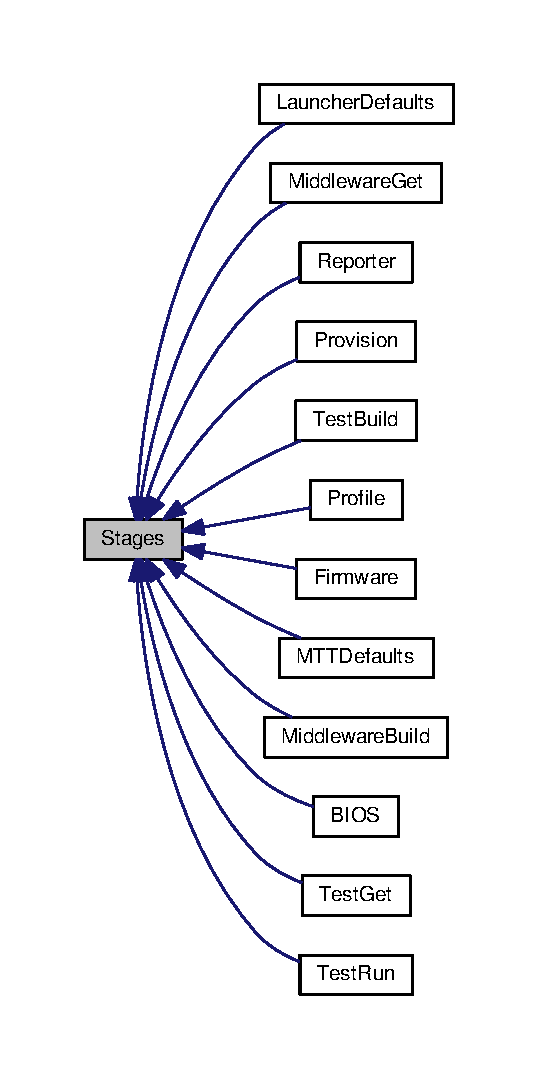
\includegraphics[width=258pt]{group__Stages}
\end{center}
\end{figure}
\subsection*{Modules}
\begin{DoxyCompactItemize}
\item 
\hyperlink{group__BIOS}{B\-I\-O\-S}
\begin{DoxyCompactList}\small\item\em ordering 50 \end{DoxyCompactList}\item 
\hyperlink{group__Firmware}{Firmware}
\begin{DoxyCompactList}\small\item\em ordering 100 \end{DoxyCompactList}\item 
\hyperlink{group__LauncherDefaults}{Launcher\-Defaults}
\begin{DoxyCompactList}\small\item\em ordering 490 \end{DoxyCompactList}\item 
\hyperlink{group__MiddlewareBuild}{Middleware\-Build}
\begin{DoxyCompactList}\small\item\em ordering 400 \end{DoxyCompactList}\item 
\hyperlink{group__MiddlewareGet}{Middleware\-Get}
\begin{DoxyCompactList}\small\item\em ordering 300 \end{DoxyCompactList}\item 
\hyperlink{group__MTTDefaults}{M\-T\-T\-Defaults}
\begin{DoxyCompactList}\small\item\em ordering 0 \end{DoxyCompactList}\item 
\hyperlink{group__Profile}{Profile}
\begin{DoxyCompactList}\small\item\em ordering 210 \end{DoxyCompactList}\item 
\hyperlink{group__Provision}{Provision}
\begin{DoxyCompactList}\small\item\em ordering 200 \end{DoxyCompactList}\item 
\hyperlink{group__Reporter}{Reporter}
\begin{DoxyCompactList}\small\item\em ordering 600 \end{DoxyCompactList}\item 
\hyperlink{group__TestBuild}{Test\-Build}
\begin{DoxyCompactList}\small\item\em ordering 475 \end{DoxyCompactList}\item 
\hyperlink{group__TestGet}{Test\-Get}
\begin{DoxyCompactList}\small\item\em ordering 450 \end{DoxyCompactList}\item 
\hyperlink{group__TestRun}{Test\-Run}
\begin{DoxyCompactList}\small\item\em ordering 500 \end{DoxyCompactList}\end{DoxyCompactItemize}


\subsection{Detailed Description}
Stages of test execution. 
\hypertarget{group__BIOS}{\section{B\-I\-O\-S}
\label{group__BIOS}\index{B\-I\-O\-S@{B\-I\-O\-S}}
}


ordering 50  


Collaboration diagram for B\-I\-O\-S\-:
\nopagebreak
\begin{figure}[H]
\begin{center}
\leavevmode
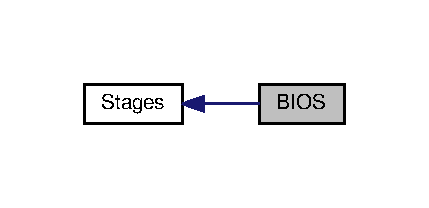
\includegraphics[width=206pt]{group__BIOS}
\end{center}
\end{figure}
ordering 50 
\hypertarget{group__Firmware}{\section{Firmware}
\label{group__Firmware}\index{Firmware@{Firmware}}
}


\mbox{[}Ordering 100\mbox{]} Firmware flash and query stage  


Collaboration diagram for Firmware\-:
\nopagebreak
\begin{figure}[H]
\begin{center}
\leavevmode
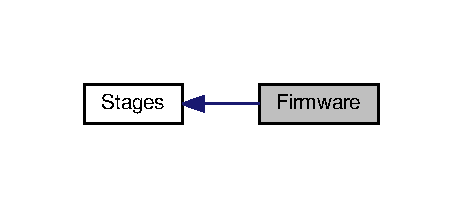
\includegraphics[width=222pt]{group__Firmware}
\end{center}
\end{figure}
\mbox{[}Ordering 100\mbox{]} Firmware flash and query stage \hypertarget{FooFlash.py_FooFlash}{}\subsection{Foo\-Flash}\label{FooFlash.py_FooFlash}

\hypertarget{group__LauncherDefaults}{\section{Launcher\-Defaults}
\label{group__LauncherDefaults}\index{Launcher\-Defaults@{Launcher\-Defaults}}
}


ordering 490  


Collaboration diagram for Launcher\-Defaults\-:
\nopagebreak
\begin{figure}[H]
\begin{center}
\leavevmode
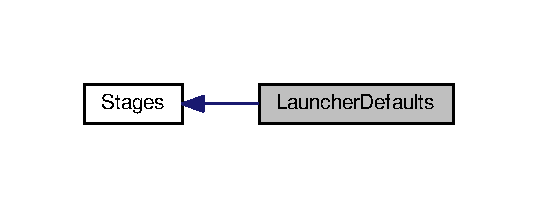
\includegraphics[width=258pt]{group__LauncherDefaults}
\end{center}
\end{figure}
ordering 490 
\hypertarget{group__MiddlewareBuild}{\section{Middleware\-Build}
\label{group__MiddlewareBuild}\index{Middleware\-Build@{Middleware\-Build}}
}


\mbox{[}Ordering 400\mbox{]} Stage for building middleware such as M\-P\-I  


Collaboration diagram for Middleware\-Build\-:
\nopagebreak
\begin{figure}[H]
\begin{center}
\leavevmode
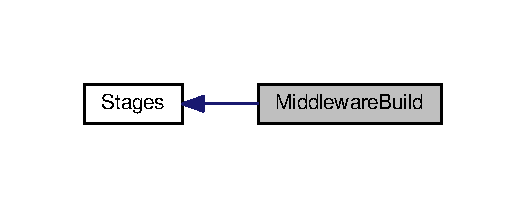
\includegraphics[width=252pt]{group__MiddlewareBuild}
\end{center}
\end{figure}
\mbox{[}Ordering 400\mbox{]} Stage for building middleware such as M\-P\-I 
\hypertarget{group__MiddlewareGet}{\section{Middleware\-Get}
\label{group__MiddlewareGet}\index{Middleware\-Get@{Middleware\-Get}}
}


\mbox{[}Ordering 300\mbox{]} Stage for getting middleware source code  


Collaboration diagram for Middleware\-Get\-:
\nopagebreak
\begin{figure}[H]
\begin{center}
\leavevmode
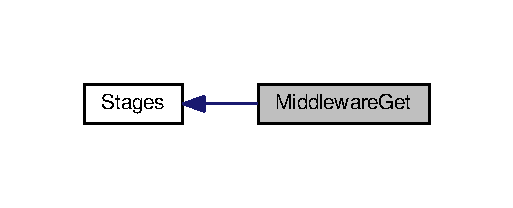
\includegraphics[width=246pt]{group__MiddlewareGet}
\end{center}
\end{figure}
\mbox{[}Ordering 300\mbox{]} Stage for getting middleware source code 
\hypertarget{group__MTTDefaults}{\section{M\-T\-T\-Defaults}
\label{group__MTTDefaults}\index{M\-T\-T\-Defaults@{M\-T\-T\-Defaults}}
}


\mbox{[}Ordering 0\mbox{]} Set M\-T\-T defaults for this test definition  


Collaboration diagram for M\-T\-T\-Defaults\-:
\nopagebreak
\begin{figure}[H]
\begin{center}
\leavevmode
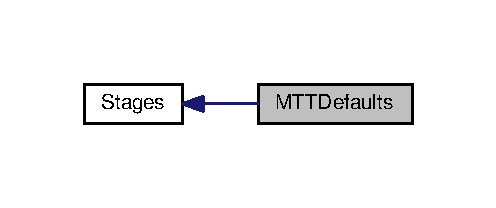
\includegraphics[width=238pt]{group__MTTDefaults}
\end{center}
\end{figure}
\mbox{[}Ordering 0\mbox{]} Set M\-T\-T defaults for this test definition \hypertarget{group__MTTDefaults_DefaultMTTDefaults}{}\subsection{Default\-M\-T\-T\-Defaults}\label{group__MTTDefaults_DefaultMTTDefaults}
Store any provided default M\-T\-T settings 
\begin{DoxyParams}{Parameters}
{\em trial} & Use when testing your M\-T\-T client setup; results that are generated and submitted to the database are marked as "trials" and are not included in normal reporting. \\
\hline
{\em scratch} & Specify the D\-I\-R\-E\-C\-T\-O\-R\-Y under which scratch files are to be stored \\
\hline
{\em description} & Provide a brief title/description to be included in the log for this test \\
\hline
{\em platform} & Name of the system under test \\
\hline
{\em organization} & Name of the organization running the test \\
\hline
{\em merge\-\_\-stdout\-\_\-stderr} & Merge stdout and stderr into one output stream \\
\hline
{\em stdout\-\_\-save\-\_\-lines} & Number of lines of stdout to save (-\/1 for unlimited) \\
\hline
{\em stderr\-\_\-save\-\_\-lines} & Number of lines of stderr to save (-\/1 for unlimited) \\
\hline
{\em executor} & Strategy to use\-: combinatorial or sequential executor \\
\hline
{\em time} & Record how long it takes to run each individual test \\
\hline
\end{DoxyParams}

\hypertarget{group__Profile}{\section{Profile}
\label{group__Profile}\index{Profile@{Profile}}
}


ordering 210  


Collaboration diagram for Profile\-:
\nopagebreak
\begin{figure}[H]
\begin{center}
\leavevmode
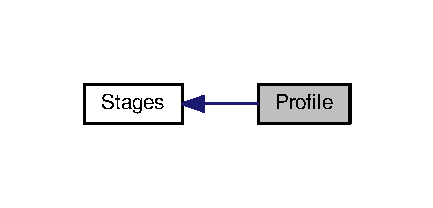
\includegraphics[width=208pt]{group__Profile}
\end{center}
\end{figure}
ordering 210 \hypertarget{group__Profile_DefaultProfile}{}\subsection{Default\-Profile}\label{group__Profile_DefaultProfile}

\begin{DoxyParams}{Parameters}
{\em kernel\-Name} & Kernel name \\
\hline
{\em kernel\-Release} & Kernel release string \\
\hline
{\em kernel\-Version} & Kernel version string \\
\hline
{\em machine\-Name} & Machine name \\
\hline
{\em processor\-Type} & Processor type \\
\hline
{\em node\-Name} & Node name \\
\hline
\end{DoxyParams}

\hypertarget{group__Provision}{\section{Provision}
\label{group__Provision}\index{Provision@{Provision}}
}


ordering 200  


Collaboration diagram for Provision\-:
\nopagebreak
\begin{figure}[H]
\begin{center}
\leavevmode
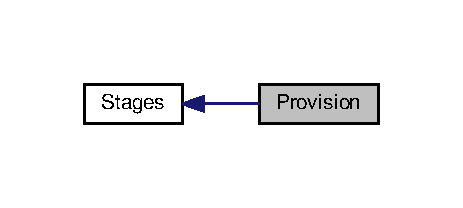
\includegraphics[width=222pt]{group__Provision}
\end{center}
\end{figure}
ordering 200 \hypertarget{group__Provision_WWulf3}{}\subsection{W\-Wulf3}\label{group__Provision_WWulf3}

\begin{DoxyParams}{Parameters}
{\em target} & List of remote host names or L\-A\-N interfaces to be provisioned \\
\hline
{\em image} & Name of image to be instantiated \\
\hline
{\em bootstrap} & Name of bootstrap to be used \\
\hline
{\em controller} & List of I\-P addresses of remote node controllers/\-B\-M\-Cs \\
\hline
{\em username} & Remote controller username \\
\hline
{\em password} & Remote controller password \\
\hline
{\em pwfile} & File containing remote controller password \\
\hline
{\em sudo} & Use sudo to execute privileged commands \\
\hline
{\em allocate\-\_\-cmd} & Command to use for allocating nodes from the resource manager \\
\hline
{\em deallocate\-\_\-cmd} & Command to use for deallocating nodes from the resource manager \\
\hline
\end{DoxyParams}

\hypertarget{group__Reporter}{\section{Reporter}
\label{group__Reporter}\index{Reporter@{Reporter}}
}


ordering 600  


Collaboration diagram for Reporter\-:
\nopagebreak
\begin{figure}[H]
\begin{center}
\leavevmode
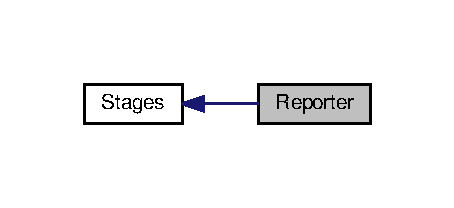
\includegraphics[width=218pt]{group__Reporter}
\end{center}
\end{figure}
ordering 600 \hypertarget{group__Reporter_IUDatabase}{}\subsection{I\-U\-Database}\label{group__Reporter_IUDatabase}

\begin{DoxyParams}{Parameters}
{\em realm} & Database name \\
\hline
{\em username} & Username to be used for submitting data \\
\hline
{\em password} & Password for that username \\
\hline
{\em pwfile} & File where password can be found \\
\hline
{\em platform} & Name of the platform (cluster) upon which the tests were run \\
\hline
{\em hostname} & Name of the hosts involved in the tests (may be regular expression) \\
\hline
{\em url} & U\-R\-L of the database server \\
\hline
{\em debug\-\_\-filename} & Debug output file for server interaction information \\
\hline
{\em keep\-\_\-debug\-\_\-files} & Retain reporter debug output after execution \\
\hline
{\em debug\-\_\-server} & Ask the server to return its debug output as well \\
\hline
{\em email} & Email to which errors are to be sent\\
\hline
\end{DoxyParams}
\hypertarget{group__Reporter_JunitXML}{}\subsection{Junit\-X\-M\-L}\label{group__Reporter_JunitXML}

\begin{DoxyParams}{Parameters}
{\em filename} & Name of the file into which the report is to be written \\
\hline
{\em textwrap} & Max line length before wrapping\\
\hline
\end{DoxyParams}
\hypertarget{group__Reporter_TextFile}{}\subsection{Text\-File}\label{group__Reporter_TextFile}

\begin{DoxyParams}{Parameters}
{\em filename} & Name of the file into which the report is to be written \\
\hline
{\em summary\-\_\-footer} & Footer to be placed at bottom of summary \\
\hline
{\em detail\-\_\-header} & Header to be put at top of detail report \\
\hline
{\em detail\-\_\-footer} & Footer to be placed at bottome of detail report \\
\hline
{\em textwrap} & Max line length before wrapping \\
\hline
\end{DoxyParams}

\hypertarget{group__TestBuild}{\section{Test\-Build}
\label{group__TestBuild}\index{Test\-Build@{Test\-Build}}
}


ordering 475  


Collaboration diagram for Test\-Build\-:
\nopagebreak
\begin{figure}[H]
\begin{center}
\leavevmode
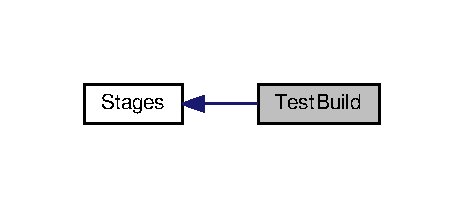
\includegraphics[width=222pt]{group__TestBuild}
\end{center}
\end{figure}
ordering 475 
\hypertarget{group__TestGet}{\section{Test\-Get}
\label{group__TestGet}\index{Test\-Get@{Test\-Get}}
}


ordering 450  


Collaboration diagram for Test\-Get\-:
\nopagebreak
\begin{figure}[H]
\begin{center}
\leavevmode
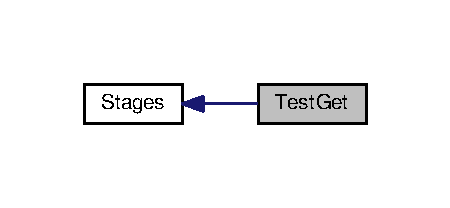
\includegraphics[width=216pt]{group__TestGet}
\end{center}
\end{figure}
ordering 450 
\hypertarget{group__TestRun}{\section{Test\-Run}
\label{group__TestRun}\index{Test\-Run@{Test\-Run}}
}


\mbox{[}Ordering 500\mbox{]} Run test software package  


Collaboration diagram for Test\-Run\-:
\nopagebreak
\begin{figure}[H]
\begin{center}
\leavevmode
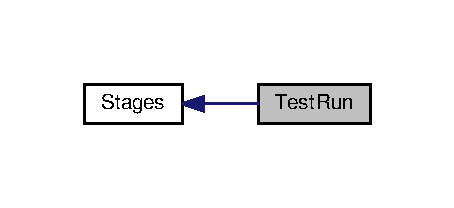
\includegraphics[width=218pt]{group__TestRun}
\end{center}
\end{figure}
\mbox{[}Ordering 500\mbox{]} Run test software package 
\hypertarget{group__Tools}{\section{Tools}
\label{group__Tools}\index{Tools@{Tools}}
}


Plugins required by Stages.  


Collaboration diagram for Tools\-:
\nopagebreak
\begin{figure}[H]
\begin{center}
\leavevmode
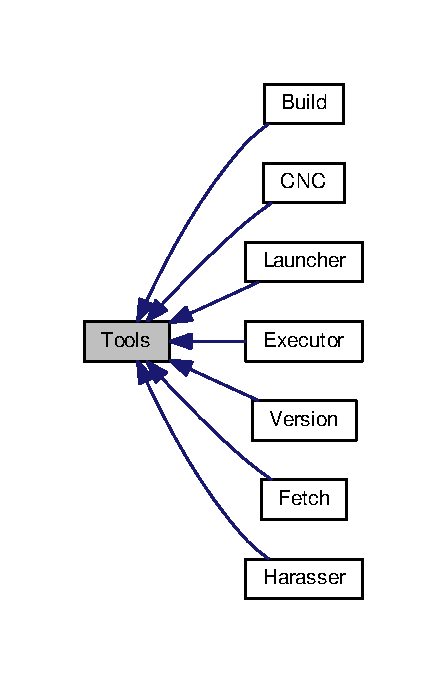
\includegraphics[width=214pt]{group__Tools}
\end{center}
\end{figure}
\subsection*{Modules}
\begin{DoxyCompactItemize}
\item 
\hyperlink{group__Build}{Build}
\begin{DoxyCompactList}\small\item\em Build tools for test content. \end{DoxyCompactList}\item 
\hyperlink{group__CNC}{C\-N\-C}
\begin{DoxyCompactList}\small\item\em Comand and control tools for system managment. \end{DoxyCompactList}\item 
\hyperlink{group__Executor}{Executor}
\begin{DoxyCompactList}\small\item\em Executor of test description. \end{DoxyCompactList}\item 
\hyperlink{group__Fetch}{Fetch}
\begin{DoxyCompactList}\small\item\em Tools for fetching tests. \end{DoxyCompactList}\item 
\hyperlink{group__Harasser}{Harasser}
\begin{DoxyCompactList}\small\item\em \hyperlink{namespaceHarasser}{Harasser} tools for test content. \end{DoxyCompactList}\item 
\hyperlink{group__Launcher}{Launcher}
\begin{DoxyCompactList}\small\item\em Tools for launching H\-P\-C jobs. \end{DoxyCompactList}\item 
\hyperlink{group__Version}{Version}
\begin{DoxyCompactList}\small\item\em Tools that collect version information. \end{DoxyCompactList}\end{DoxyCompactItemize}


\subsection{Detailed Description}
Plugins required by Stages. 
\hypertarget{group__Utilities}{\section{Utilities}
\label{group__Utilities}\index{Utilities@{Utilities}}
}


Plugins used by the M\-T\-T framework.  


Plugins used by the M\-T\-T framework. \hypertarget{group__Utilities_Compilers}{}\subsection{Compilers}\label{group__Utilities_Compilers}
Identify the type and version of compilers in-\/use\hypertarget{group__Utilities_Copytree}{}\subsection{Copytree}\label{group__Utilities_Copytree}
Copy a directory tree from source to the same relative loation under the M\-T\-T scratch directory 
\begin{DoxyParams}{Parameters}
{\em src} & The top directory of the tree to be copied \\
\hline
{\em preserve\-\_\-symlinks} & Preserve symlinks instead of copying the contents \\
\hline
{\em preserve\-\_\-directory} & Copies directory instead of contents\\
\hline
\end{DoxyParams}
\hypertarget{group__Utilities_Environ}{}\subsection{Environ}\label{group__Utilities_Environ}
Set environment variables\hypertarget{group__Utilities_ExecuteCmd}{}\subsection{Execute\-Cmd}\label{group__Utilities_ExecuteCmd}
Execute a command and capture its stdout and stderr\hypertarget{group__Utilities_Logger}{}\subsection{Logger}\label{group__Utilities_Logger}
Log results and provide debug output when directed\hypertarget{group__Utilities_ModuleCmd}{}\subsection{Module\-Cmd}\label{group__Utilities_ModuleCmd}
Load/\-Unload an environmental module\hypertarget{group__Utilities_MPIVersion}{}\subsection{M\-P\-I\-Version}\label{group__Utilities_MPIVersion}
Identify the name and version of M\-P\-I in-\/use\hypertarget{group__Utilities_Watchdog}{}\subsection{Watchdog}\label{group__Utilities_Watchdog}
Generate and exception after a given amount of time 
\begin{DoxyParams}{Parameters}
{\em timeout} & Time in seconds before generating exception \\
\hline
\end{DoxyParams}

\hypertarget{group__Build}{\section{Build}
\label{group__Build}\index{Build@{Build}}
}


Build tools for test content.  


Collaboration diagram for Build\-:
\nopagebreak
\begin{figure}[H]
\begin{center}
\leavevmode
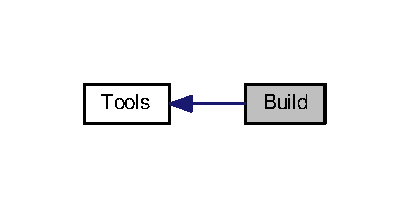
\includegraphics[width=196pt]{group__Build}
\end{center}
\end{figure}
Build tools for test content. \hypertarget{group__Build_Autotools}{}\subsection{Autotools}\label{group__Build_Autotools}

\begin{DoxyParams}{Parameters}
{\em middleware} & Middleware stage that these tests are to be built against \\
\hline
{\em parent} & Section that precedes this one in the dependency tree \\
\hline
{\em autogen\-\_\-cmd} & Command to be executed to setup the configure script, usually called autogen.\-sh or autogen.\-pl \\
\hline
{\em configure\-\_\-options} & Options to be passed to configure. Note that the prefix will be automatically set and need not be provided here \\
\hline
{\em make\-\_\-options} & Options to be passed to the make command \\
\hline
{\em build\-\_\-in\-\_\-place} & Build tests in current location (no prefix or install) \\
\hline
{\em merge\-\_\-stdout\-\_\-stderr} & Merge stdout and stderr into one output stream \\
\hline
{\em stdout\-\_\-save\-\_\-lines} & Number of lines of stdout to save \\
\hline
{\em stderr\-\_\-save\-\_\-lines} & Number of lines of stderr to save \\
\hline
{\em modules} & Modules to load \\
\hline
{\em modules\-\_\-unload} & Modules to unload\\
\hline
\end{DoxyParams}
\hypertarget{group__Build_Hostfile}{}\subsection{Hostfile}\label{group__Build_Hostfile}

\begin{DoxyParams}{Parameters}
{\em parent} & Section that precedes this one in the dependency tree \\
\hline
{\em nodelist} & list of nodes to create hostfile from \\
\hline
{\em hostfile} & name of hostfile to generate\\
\hline
\end{DoxyParams}
\hypertarget{group__Build_Shell}{}\subsection{Shell}\label{group__Build_Shell}

\begin{DoxyParams}{Parameters}
{\em middleware} & Middleware stage that these tests are to be built against \\
\hline
{\em command} & Command to execute \\
\hline
{\em parent} & Section that precedes this one in the dependency tree \\
\hline
{\em merge\-\_\-stdout\-\_\-stderr} & Merge stdout and stderr into one output stream \\
\hline
{\em stdout\-\_\-save\-\_\-lines} & Number of lines of stdout to save \\
\hline
{\em stderr\-\_\-save\-\_\-lines} & Number of lines of stderr to save \\
\hline
{\em modules} & Modules to load \\
\hline
{\em modules\-\_\-unload} & Modules to unload \\
\hline
{\em fail\-\_\-test} & Specifies whether this test is expected to fail (value=None means test is expected to succeed) \\
\hline
{\em fail\-\_\-returncode} & Specifies the expected failure returncode of this test \\
\hline
{\em allocate\-\_\-cmd} & Command to use for allocating nodes from the resource manager \\
\hline
{\em deallocate\-\_\-cmd} & Command to use for deallocating nodes from the resource manager \\
\hline
{\em asis\-\_\-target} & Specifies name of asis\-\_\-target being built. This is used with "A\-S\-I\-S" keyword to determine whether to do anything. \\
\hline
\end{DoxyParams}

\hypertarget{group__CNC}{\section{C\-N\-C}
\label{group__CNC}\index{C\-N\-C@{C\-N\-C}}
}


Comand and control tools for system managment.  


Collaboration diagram for C\-N\-C\-:
\nopagebreak
\begin{figure}[H]
\begin{center}
\leavevmode
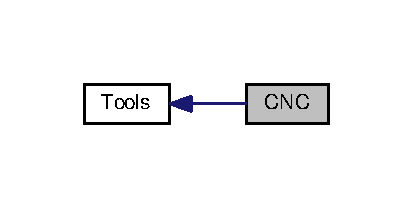
\includegraphics[width=198pt]{group__CNC}
\end{center}
\end{figure}
Comand and control tools for system managment. \hypertarget{group__CNC_IPMITool}{}\subsection{I\-P\-M\-I\-Tool}\label{group__CNC_IPMITool}

\begin{DoxyParams}{Parameters}
{\em target} & List of remote host names or L\-A\-N interfaces to monitor during reset operations \\
\hline
{\em controller} & List of I\-P addresses of remote node controllers/\-B\-M\-Cs \\
\hline
{\em username} & Remote session username \\
\hline
{\em password} & Remote session password \\
\hline
{\em pwfile} & File containing remote session password \\
\hline
{\em command} & Command to be sent \\
\hline
{\em maxtries} & Max number of times to ping each host before declaring reset to fail \\
\hline
{\em numthreads} & Number of worker threads to use \\
\hline
{\em dryrun} & Dryrun -\/ print out commands but do not execute \\
\hline
{\em sudo} & Use sudo to exeute privilaged comands \\
\hline
\end{DoxyParams}

\hypertarget{group__Executor}{\section{Executor}
\label{group__Executor}\index{Executor@{Executor}}
}


Executor of test description.  


Collaboration diagram for Executor\-:
\nopagebreak
\begin{figure}[H]
\begin{center}
\leavevmode
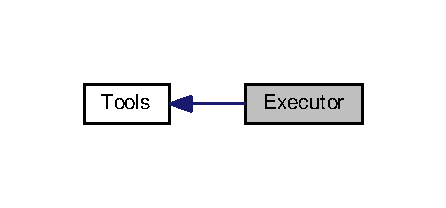
\includegraphics[width=214pt]{group__Executor}
\end{center}
\end{figure}
Executor of test description. \hypertarget{group__Executor_CombinatorialEx}{}\subsection{Combinatorial\-Ex}\label{group__Executor_CombinatorialEx}
Combinatorial execution executor\hypertarget{group__Executor_SequentialEx}{}\subsection{Sequential\-Ex}\label{group__Executor_SequentialEx}
Sequential execution executor 
\hypertarget{group__Fetch}{\section{Fetch}
\label{group__Fetch}\index{Fetch@{Fetch}}
}


Tools for fetching tests.  


Collaboration diagram for Fetch\-:
\nopagebreak
\begin{figure}[H]
\begin{center}
\leavevmode
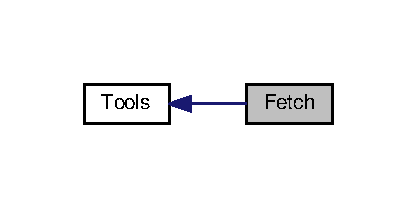
\includegraphics[width=200pt]{group__Fetch}
\end{center}
\end{figure}
Tools for fetching tests. \hypertarget{group__Fetch_AlreadyInstalled}{}\subsection{Already\-Installed}\label{group__Fetch_AlreadyInstalled}

\begin{DoxyParams}{Parameters}
{\em exec} & Executable that should be in path \\
\hline
{\em module} & Modules (or lmod modules) to be loaded for accessing this package\\
\hline
\end{DoxyParams}
\hypertarget{group__Fetch_Git}{}\subsection{Git}\label{group__Fetch_Git}

\begin{DoxyParams}{Parameters}
{\em module} & Modules (or lmod modules) to be loaded for accessing this package \\
\hline
{\em url} & U\-R\-L to access the repository \\
\hline
{\em username} & Username required for accessing the repository \\
\hline
{\em password} & Password required for that user to access the repository \\
\hline
{\em pwfile} & File where password can be found \\
\hline
{\em branch} & Branch (if not master) to be downloaded \\
\hline
{\em pr} & Pull request to be downloaded \\
\hline
{\em subdir} & Subdirectory of interest in repository\\
\hline
\end{DoxyParams}
\hypertarget{group__Fetch_OMPI_Snapshot}{}\subsection{O\-M\-P\-I\-\_\-\-Snapshot}\label{group__Fetch_OMPI_Snapshot}

\begin{DoxyParams}{Parameters}
{\em url} & U\-R\-L to access the O\-M\-P\-I nightly tarball (e.\-g. \href{https://www.open-mpi.org/nightly/v2.x}{\tt https\-://www.\-open-\/mpi.\-org/nightly/v2.\-x}) \\
\hline
{\em version\-\_\-file} & optional file containing name of most recent tarball version tested \\
\hline
{\em mpi\-\_\-name} & optional name for the O\-M\-P\-I snapshot tarball \\
\hline
\end{DoxyParams}

\hypertarget{group__Harasser}{\section{Harasser}
\label{group__Harasser}\index{Harasser@{Harasser}}
}


\hyperlink{namespaceHarasser}{Harasser} tools for test content.  


Collaboration diagram for Harasser\-:
\nopagebreak
\begin{figure}[H]
\begin{center}
\leavevmode
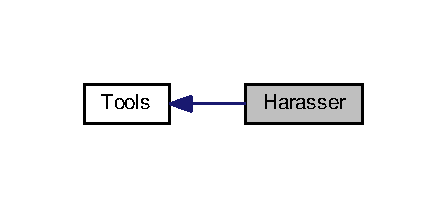
\includegraphics[width=214pt]{group__Harasser}
\end{center}
\end{figure}
\hyperlink{namespaceHarasser}{Harasser} tools for test content. \hypertarget{group__Harasser_Harasser}{}\subsection{Harasser}\label{group__Harasser_Harasser}

\begin{DoxyParams}{Parameters}
{\em trigger\-\_\-scripts} & Scripts to run to launch harassers \\
\hline
{\em stop\-\_\-scripts} & Scripts to run to stop and clean-\/up harassers \\
\hline
{\em join\-\_\-timeout} & Seconds to wait for process to finish \\
\hline
\end{DoxyParams}

\hypertarget{group__Launcher}{\section{Launcher}
\label{group__Launcher}\index{Launcher@{Launcher}}
}


Tools for launching H\-P\-C jobs.  


Collaboration diagram for Launcher\-:
\nopagebreak
\begin{figure}[H]
\begin{center}
\leavevmode
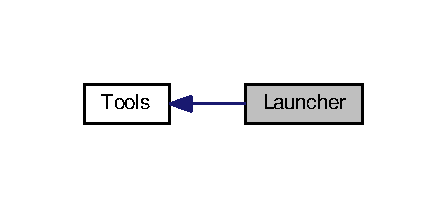
\includegraphics[width=214pt]{group__Launcher}
\end{center}
\end{figure}
Tools for launching H\-P\-C jobs. \hypertarget{group__Launcher_ALPS}{}\subsection{A\-L\-P\-S}\label{group__Launcher_ALPS}
Plugin for using \hyperlink{namespaceALPS}{A\-L\-P\-S} to launch tests 
\begin{DoxyParams}{Parameters}
{\em hostfile} & The hostfile for \hyperlink{namespaceOpenMPI}{Open\-M\-P\-I} to use \\
\hline
{\em command} & Command for executing the application \\
\hline
{\em np} & Number of processes to run \\
\hline
{\em options} & Comma-\/delimited sets of command line options that shall be used on each test \\
\hline
{\em skipped} & Exit status of a test that declares it was skipped \\
\hline
{\em merge\-\_\-stdout\-\_\-stderr} & Merge stdout and stderr into one output stream \\
\hline
{\em stdout\-\_\-save\-\_\-lines} & Number of lines of stdout to save \\
\hline
{\em stderr\-\_\-save\-\_\-lines} & Number of lines of stderr to save \\
\hline
{\em test\-\_\-dir} & Names of directories to be scanned for tests \\
\hline
{\em fail\-\_\-tests} & Names of tests that are expected to fail \\
\hline
{\em fail\-\_\-returncodes} & Expected returncodes of tests expected to fail \\
\hline
{\em fail\-\_\-timeout} & Maximum execution time for tests expected to fail \\
\hline
{\em skip\-\_\-tests} & Names of tests to be skipped \\
\hline
{\em max\-\_\-num\-\_\-tests} & Maximum number of tests to run \\
\hline
{\em modules} & Modules to load \\
\hline
{\em modules\-\_\-unload} & Modules to unload \\
\hline
{\em test\-\_\-list} & List of tests to run, default is all \\
\hline
{\em allocate\-\_\-cmd} & Command to use for allocating nodes from the resource manager \\
\hline
{\em deallocate\-\_\-cmd} & Command to use for deallocating nodes from the resource manager\\
\hline
\end{DoxyParams}
\hypertarget{group__Launcher_OpenMPI}{}\subsection{Open\-M\-P\-I}\label{group__Launcher_OpenMPI}
Plugin for using the Open M\-P\-I mpirun launch tool 
\begin{DoxyParams}{Parameters}
{\em hostfile} & The hostfile for \hyperlink{namespaceOpenMPI}{Open\-M\-P\-I} to use \\
\hline
{\em command} & Command for executing the application \\
\hline
{\em np} & Number of processes to run \\
\hline
{\em ppn} & Number of processes per node to run \\
\hline
{\em timeout} & Maximum execution time -\/ terminate a test if it exceeds this time \\
\hline
{\em options} & Comma-\/delimited sets of command line options that shall be used on each test \\
\hline
{\em skipped} & Exit status of a test that declares it was skipped \\
\hline
{\em merge\-\_\-stdout\-\_\-stderr} & Merge stdout and stderr into one output stream \\
\hline
{\em stdout\-\_\-save\-\_\-lines} & Number of lines of stdout to save \\
\hline
{\em stderr\-\_\-save\-\_\-lines} & Number of lines of stderr to save \\
\hline
{\em test\-\_\-dir} & Names of directories to be scanned for tests \\
\hline
{\em fail\-\_\-tests} & Names of tests that are expected to fail \\
\hline
{\em fail\-\_\-returncodes} & Expected return codes of tests expected to fail \\
\hline
{\em fail\-\_\-timeout} & Maximum execution time for tests expected to fail \\
\hline
{\em skip\-\_\-tests} & Names of tests to be skipped \\
\hline
{\em max\-\_\-num\-\_\-tests} & Maximum number of tests to run \\
\hline
{\em test\-\_\-list} & List of tests to run, default is all \\
\hline
{\em allocate\-\_\-cmd} & Command to use for allocating nodes from the resource manager \\
\hline
{\em deallocate\-\_\-cmd} & Command to use for deallocating nodes from the resource manager\\
\hline
\end{DoxyParams}
\hypertarget{group__Launcher_SLURM}{}\subsection{S\-L\-U\-R\-M}\label{group__Launcher_SLURM}
Plugin for using \hyperlink{namespaceSLURM}{S\-L\-U\-R\-M} to launch tests 
\begin{DoxyParams}{Parameters}
{\em hostfile} & The hostfile for \hyperlink{namespaceOpenMPI}{Open\-M\-P\-I} to use \\
\hline
{\em command} & Command for executing the application \\
\hline
{\em np} & Number of processes to run \\
\hline
{\em timeout} & Maximum execution time -\/ terminate a test if it exceeds this time \\
\hline
{\em options} & Comma-\/delimited sets of command line options that shall be used on each test \\
\hline
{\em skipped} & Exit status of a test that declares it was skipped \\
\hline
{\em merge\-\_\-stdout\-\_\-stderr} & Merge stdout and stderr into one output stream \\
\hline
{\em stdout\-\_\-save\-\_\-lines} & Number of lines of stdout to save \\
\hline
{\em stderr\-\_\-save\-\_\-lines} & Number of lines of stderr to save \\
\hline
{\em test\-\_\-dir} & Names of directories to be scanned for tests \\
\hline
{\em fail\-\_\-tests} & Names of tests that are expected to fail \\
\hline
{\em fail\-\_\-returncodes} & Expected returncodes of tests expected to fail \\
\hline
{\em fail\-\_\-timeout} & Maximum execution time for tests expected to fail \\
\hline
{\em skip\-\_\-tests} & Names of tests to be skipped \\
\hline
{\em max\-\_\-num\-\_\-tests} & Maximum number of tests to run \\
\hline
{\em job\-\_\-name} & User-\/defined name for job \\
\hline
{\em modules} & Modules to load \\
\hline
{\em modules\-\_\-unload} & Modules to unload \\
\hline
{\em test\-\_\-list} & List of tests to run, default is all \\
\hline
{\em allocate\-\_\-cmd} & Command to use for allocating nodes from the resource manager \\
\hline
{\em deallocate\-\_\-cmd} & Command to use for deallocating nodes from the resource manager \\
\hline
\end{DoxyParams}

\hypertarget{group__Version}{\section{Version}
\label{group__Version}\index{Version@{Version}}
}


Tools that collect version information.  


Collaboration diagram for Version\-:
\nopagebreak
\begin{figure}[H]
\begin{center}
\leavevmode
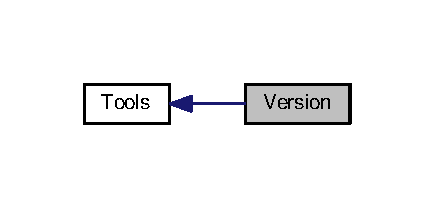
\includegraphics[width=208pt]{group__Version}
\end{center}
\end{figure}
Tools that collect version information. \hypertarget{MTTVersionPlugin.py_MTTVersionPlugin}{}\subsection{M\-T\-T\-Version\-Plugin}\label{MTTVersionPlugin.py_MTTVersionPlugin}

\chapter{Namespace Documentation}
\hypertarget{namespaceALPS}{\section{A\-L\-P\-S Namespace Reference}
\label{namespaceALPS}\index{A\-L\-P\-S@{A\-L\-P\-S}}
}

\hypertarget{namespaceAlreadyInstalled}{\section{Already\-Installed Namespace Reference}
\label{namespaceAlreadyInstalled}\index{Already\-Installed@{Already\-Installed}}
}
\subsection*{Classes}
\begin{DoxyCompactItemize}
\item 
class \hyperlink{classAlreadyInstalled_1_1AlreadyInstalled}{Already\-Installed}
\end{DoxyCompactItemize}

\hypertarget{namespaceAutotools}{\section{Autotools Namespace Reference}
\label{namespaceAutotools}\index{Autotools@{Autotools}}
}
\subsection*{Classes}
\begin{DoxyCompactItemize}
\item 
class \hyperlink{classAutotools_1_1Autotools}{Autotools}
\end{DoxyCompactItemize}

\hypertarget{namespaceBaseMTTUtility}{\section{Base\-M\-T\-T\-Utility Namespace Reference}
\label{namespaceBaseMTTUtility}\index{Base\-M\-T\-T\-Utility@{Base\-M\-T\-T\-Utility}}
}

\hypertarget{namespaceBIOSMTTStage}{\section{B\-I\-O\-S\-M\-T\-T\-Stage Namespace Reference}
\label{namespaceBIOSMTTStage}\index{B\-I\-O\-S\-M\-T\-T\-Stage@{B\-I\-O\-S\-M\-T\-T\-Stage}}
}
\subsection*{Classes}
\begin{DoxyCompactItemize}
\item 
class \hyperlink{classBIOSMTTStage_1_1BIOSMTTStage}{B\-I\-O\-S\-M\-T\-T\-Stage}
\end{DoxyCompactItemize}

\hypertarget{namespaceBuildMTTTool}{\section{Build\-M\-T\-T\-Tool Namespace Reference}
\label{namespaceBuildMTTTool}\index{Build\-M\-T\-T\-Tool@{Build\-M\-T\-T\-Tool}}
}
\subsection*{Classes}
\begin{DoxyCompactItemize}
\item 
class \hyperlink{classBuildMTTTool_1_1BuildMTTTool}{Build\-M\-T\-T\-Tool}
\end{DoxyCompactItemize}

\hypertarget{namespaceCheckProfile}{\section{Check\-Profile Namespace Reference}
\label{namespaceCheckProfile}\index{Check\-Profile@{Check\-Profile}}
}

\hypertarget{namespaceCNCMTTTool}{\section{C\-N\-C\-M\-T\-T\-Tool Namespace Reference}
\label{namespaceCNCMTTTool}\index{C\-N\-C\-M\-T\-T\-Tool@{C\-N\-C\-M\-T\-T\-Tool}}
}

\hypertarget{namespacecombinatorial}{\section{combinatorial Namespace Reference}
\label{namespacecombinatorial}\index{combinatorial@{combinatorial}}
}
\subsection*{Classes}
\begin{DoxyCompactItemize}
\item 
class \hyperlink{classcombinatorial_1_1CombinatorialEx}{Combinatorial\-Ex}
\end{DoxyCompactItemize}

\hypertarget{namespaceCompilers}{\section{Compilers Namespace Reference}
\label{namespaceCompilers}\index{Compilers@{Compilers}}
}

\hypertarget{namespaceCopytree}{\section{Copytree Namespace Reference}
\label{namespaceCopytree}\index{Copytree@{Copytree}}
}

\hypertarget{namespaceDefaultMTTDefaults}{\section{Default\-M\-T\-T\-Defaults Namespace Reference}
\label{namespaceDefaultMTTDefaults}\index{Default\-M\-T\-T\-Defaults@{Default\-M\-T\-T\-Defaults}}
}

\hypertarget{namespaceDefaultProfile}{\section{Default\-Profile Namespace Reference}
\label{namespaceDefaultProfile}\index{Default\-Profile@{Default\-Profile}}
}

\hypertarget{namespaceDefaultTestBuild}{\section{Default\-Test\-Build Namespace Reference}
\label{namespaceDefaultTestBuild}\index{Default\-Test\-Build@{Default\-Test\-Build}}
}
\subsection*{Classes}
\begin{DoxyCompactItemize}
\item 
class \hyperlink{classDefaultTestBuild_1_1DefaultTestBuild}{Default\-Test\-Build}
\end{DoxyCompactItemize}

\hypertarget{namespacedeveloper}{\section{developer Namespace Reference}
\label{namespacedeveloper}\index{developer@{developer}}
}

\hypertarget{namespaceEnviron}{\section{Environ Namespace Reference}
\label{namespaceEnviron}\index{Environ@{Environ}}
}

\hypertarget{namespaceExecuteCmd}{\section{Execute\-Cmd Namespace Reference}
\label{namespaceExecuteCmd}\index{Execute\-Cmd@{Execute\-Cmd}}
}

\hypertarget{namespaceExecutorMTTTool}{\section{Executor\-M\-T\-T\-Tool Namespace Reference}
\label{namespaceExecutorMTTTool}\index{Executor\-M\-T\-T\-Tool@{Executor\-M\-T\-T\-Tool}}
}

\hypertarget{namespaceFetchMTTTool}{\section{Fetch\-M\-T\-T\-Tool Namespace Reference}
\label{namespaceFetchMTTTool}\index{Fetch\-M\-T\-T\-Tool@{Fetch\-M\-T\-T\-Tool}}
}
\subsection*{Classes}
\begin{DoxyCompactItemize}
\item 
class \hyperlink{classFetchMTTTool_1_1FetchMTTTool}{Fetch\-M\-T\-T\-Tool}
\end{DoxyCompactItemize}

\hypertarget{namespaceFirmwareMTTStage}{\section{Firmware\-M\-T\-T\-Stage Namespace Reference}
\label{namespaceFirmwareMTTStage}\index{Firmware\-M\-T\-T\-Stage@{Firmware\-M\-T\-T\-Stage}}
}
\subsection*{Classes}
\begin{DoxyCompactItemize}
\item 
class \hyperlink{classFirmwareMTTStage_1_1FirmwareMTTStage}{Firmware\-M\-T\-T\-Stage}
\end{DoxyCompactItemize}

\hypertarget{namespaceFooFlash}{\section{Foo\-Flash Namespace Reference}
\label{namespaceFooFlash}\index{Foo\-Flash@{Foo\-Flash}}
}

\hypertarget{namespaceftb}{\section{ftb Namespace Reference}
\label{namespaceftb}\index{ftb@{ftb}}
}

\hypertarget{namespacefull-trivial}{\section{full-\/trivial Namespace Reference}
\label{namespacefull-trivial}\index{full-\/trivial@{full-\/trivial}}
}
\subsection*{Variables}
\begin{DoxyCompactItemize}
\item 
\hyperlink{namespacefull-trivial_ad3a7f6605e8fa1721ffb53150f1b1f2b}{description} = Platform\-L\-S\-F\-Open\-M\-P\-Itesting
\item 
int \hyperlink{namespacefull-trivial_a431381ca4d3ce0533b84fdf824145c45}{trial} = 1
\item 
\hyperlink{namespacefull-trivial_ac8c1b563f56da3a28444d9ba8c6e9cc9}{mpi\-\_\-details} = O\-M\-P\-I
\item 
\hyperlink{namespacefull-trivial_ac8f46360931db54c90bacdbeb7de743d}{module} = O\-M\-P\-I\-\_\-\-Snapshot
\item 
\hyperlink{namespacefull-trivial_ad99b4206b0691dff98229634af7de89e}{ompi\-\_\-snapshot\-\_\-url} = http\-://www.\-open-\/mpi.\-org/nightly/trunk
\item 
tuple \hyperlink{namespacefull-trivial_a8cb0b5677b37b7bb5ee95a14399ff9a3}{ompi\-\_\-snapshot\-\_\-version\-\_\-file} = \&getenv(\char`\"{}H\-O\-M\-E\char`\"{})
\item 
int \hyperlink{namespacefull-trivial_a27abf09427482f97a0072b3be7e6601d}{mpi\-\_\-get} = ompi-\/nightly-\/v1.\-3
\item 
int \hyperlink{namespacefull-trivial_aa9f5860b95aa3cfb3deaa3cf840b5615}{save\-\_\-stdout\-\_\-on\-\_\-success} = 1
\item 
int \hyperlink{namespacefull-trivial_abffbc48fc37ad6d7010976ca874c845f}{merge\-\_\-stdout\-\_\-stderr} = 0
\item 
\hyperlink{namespacefull-trivial_a58c9dd08bbe532a5face257efa5cbd3e}{ompi\-\_\-vpath\-\_\-mode} = none
\item 
int \hyperlink{namespacefull-trivial_a5a973d684d1c8c9442df7cd698a3cd03}{ompi\-\_\-make\-\_\-all\-\_\-arguments} = -\/j4
\item 
int \hyperlink{namespacefull-trivial_a84b104cbca5b5b6e7d726de01ad3947f}{ompi\-\_\-make\-\_\-check} = 1
\item 
\hyperlink{namespacefull-trivial_ab1eddfc5389978f354d58c7637810d41}{ompi\-\_\-compiler\-\_\-name} = gnu
\item 
tuple \hyperlink{namespacefull-trivial_ae61160048d266c12c817f0c990b0b41b}{ompi\-\_\-compiler\-\_\-version} = \&get\-\_\-gcc\-\_\-version()
\item 
\hyperlink{namespacefull-trivial_ad846b3615dd310ecef321a446f558151}{ompi\-\_\-configure\-\_\-arguments} = $<$$<$E\-O\-T
\item 
tuple \hyperlink{namespacefull-trivial_a96c49e3c0c2dc3c6f9dbf27fe22ff837}{exec} = mpirun-\/\hyperlink{namespacefull-trivial_acf328fb05e5f171cd49e3b6930f21f2f}{np}\&test\-\_\-np()
\item 
tuple \hyperlink{namespacefull-trivial_a6513f5e0f867d0312f10064a0adb1740}{parameters}
\item 
tuple \hyperlink{namespacefull-trivial_aec768b574435ba99bb3d8737549d08e5}{network} = \&M\-P\-I\-::\-O\-M\-P\-I\-::find\-\_\-network(\&test\-\_\-command\-\_\-line(), \&test\-\_\-executable())
\item 
\hyperlink{namespacefull-trivial_a3973918af8b0679a239a862cdc097804}{test\-\_\-get} = trivial
\item 
\hyperlink{namespacefull-trivial_aa09bcc003045dcca018f705fcea70f0f}{test\-\_\-build} = trivial
\item 
tuple \hyperlink{namespacefull-trivial_a47d8fbeff54aeee0210d2f5d55d4fc75}{pass} = \&and(\&test\-\_\-wifexited(), \&eq(\&test\-\_\-wexitstatus(), 0))
\item 
int \hyperlink{namespacefull-trivial_a119af101bc6d9cb4061ffea6b4187230}{skipped} = 0
\item 
tuple \hyperlink{namespacefull-trivial_a87b2271fca0c5c5553c1a20d8ee1c11d}{timeout} = \&max(10, \&test\-\_\-np())
\item 
int \hyperlink{namespacefull-trivial_a648cfc9aa4be2d29a9b2cc7fa66a99de}{save\-\_\-stdout\-\_\-on\-\_\-pass} = 1
\item 
int \hyperlink{namespacefull-trivial_a701f09db43ab9e43a49aaf76aa97b131}{stdout\-\_\-save\-\_\-lines} = 50
\item 
int \hyperlink{namespacefull-trivial_ab88dfbf498ed0d90e1a0510bbbb706fa}{stderr\-\_\-save\-\_\-lines} = 100
\item 
tuple \hyperlink{namespacefull-trivial_acf328fb05e5f171cd49e3b6930f21f2f}{np} = \&env\-\_\-max\-\_\-procs()
\item 
\hyperlink{namespacefull-trivial_a8845e5ef8465c334338eba7b42c0c61c}{specify\-\_\-module} = Simple
\item 
\hyperlink{namespacefull-trivial_a5f93117c210f5de7bd0b75c05ca93072}{mttdatabase\-\_\-realm} = O\-M\-P\-I
\item 
\hyperlink{namespacefull-trivial_a2556ba8e56d9edb19b2a7dcff147fd83}{mttdatabase\-\_\-username} = platform
\item 
tuple \hyperlink{namespacefull-trivial_a00ca0a7632b4a85ca5df552bc984a77d}{mttdatabase\-\_\-password} = \&shell(\char`\"{}cat /home/ompitest/mtt-\/platform-\/db-\/password.\-txt\char`\"{})
\item 
int \hyperlink{namespacefull-trivial_a7435f3a6cf574a375aa8cb9b7b2fe162}{mttdatabase\-\_\-platform} = R\-H\-E\-L4
\item 
tuple \hyperlink{namespacefull-trivial_a774cf7cf721e8c1716122a628a72e4f8}{mttdatabase\-\_\-hostname} = \&shell(\char`\"{}hostname\char`\"{})
\item 
\hyperlink{namespacefull-trivial_a1e6b981d941fc6b728d6faae8632e225}{mttdatabase\-\_\-url} = https\-://www.\-open-\/mpi.\-org/mtt/submit/
\item 
\hyperlink{namespacefull-trivial_a5a952dcadcccb56251a2745399a467c5}{mttdatabase\-\_\-debug\-\_\-filename} = mttdb\-\_\-debug\-\_\-file
\item 
int \hyperlink{namespacefull-trivial_ad2a2564c1ae95fb67eda20314bac44f5}{mttdatabase\-\_\-keep\-\_\-debug\-\_\-files} = 1
\item 
int \hyperlink{namespacefull-trivial_a6ed803b39509a0e919f4f11063cb5209}{mttdatabase\-\_\-debug\-\_\-server} = 1
\end{DoxyCompactItemize}


\subsection{Variable Documentation}
\hypertarget{namespacefull-trivial_ad3a7f6605e8fa1721ffb53150f1b1f2b}{\index{full-\/trivial@{full-\/trivial}!description@{description}}
\index{description@{description}!full-trivial@{full-\/trivial}}
\subsubsection[{description}]{\setlength{\rightskip}{0pt plus 5cm}full-\/trivial.\-description = Platform\-L\-S\-F\-Open\-M\-P\-Itesting}}\label{namespacefull-trivial_ad3a7f6605e8fa1721ffb53150f1b1f2b}


Definition at line 10 of file full-\/trivial.\-ini.

\hypertarget{namespacefull-trivial_a96c49e3c0c2dc3c6f9dbf27fe22ff837}{\index{full-\/trivial@{full-\/trivial}!exec@{exec}}
\index{exec@{exec}!full-trivial@{full-\/trivial}}
\subsubsection[{exec}]{\setlength{\rightskip}{0pt plus 5cm}tuple full-\/trivial.\-exec = mpirun-\/{\bf np}\&test\-\_\-np()}}\label{namespacefull-trivial_a96c49e3c0c2dc3c6f9dbf27fe22ff837}


Definition at line 75 of file full-\/trivial.\-ini.

\hypertarget{namespacefull-trivial_abffbc48fc37ad6d7010976ca874c845f}{\index{full-\/trivial@{full-\/trivial}!merge\-\_\-stdout\-\_\-stderr@{merge\-\_\-stdout\-\_\-stderr}}
\index{merge\-\_\-stdout\-\_\-stderr@{merge\-\_\-stdout\-\_\-stderr}!full-trivial@{full-\/trivial}}
\subsubsection[{merge\-\_\-stdout\-\_\-stderr}]{\setlength{\rightskip}{0pt plus 5cm}int full-\/trivial.\-merge\-\_\-stdout\-\_\-stderr = 0}}\label{namespacefull-trivial_abffbc48fc37ad6d7010976ca874c845f}


Definition at line 52 of file full-\/trivial.\-ini.

\hypertarget{namespacefull-trivial_ac8f46360931db54c90bacdbeb7de743d}{\index{full-\/trivial@{full-\/trivial}!module@{module}}
\index{module@{module}!full-trivial@{full-\/trivial}}
\subsubsection[{module}]{\setlength{\rightskip}{0pt plus 5cm}full-\/trivial.\-module = O\-M\-P\-I\-\_\-\-Snapshot}}\label{namespacefull-trivial_ac8f46360931db54c90bacdbeb7de743d}


Definition at line 27 of file full-\/trivial.\-ini.

\hypertarget{namespacefull-trivial_ac8c1b563f56da3a28444d9ba8c6e9cc9}{\index{full-\/trivial@{full-\/trivial}!mpi\-\_\-details@{mpi\-\_\-details}}
\index{mpi\-\_\-details@{mpi\-\_\-details}!full-trivial@{full-\/trivial}}
\subsubsection[{mpi\-\_\-details}]{\setlength{\rightskip}{0pt plus 5cm}full-\/trivial.\-mpi\-\_\-details = O\-M\-P\-I}}\label{namespacefull-trivial_ac8c1b563f56da3a28444d9ba8c6e9cc9}


Definition at line 25 of file full-\/trivial.\-ini.

\hypertarget{namespacefull-trivial_a27abf09427482f97a0072b3be7e6601d}{\index{full-\/trivial@{full-\/trivial}!mpi\-\_\-get@{mpi\-\_\-get}}
\index{mpi\-\_\-get@{mpi\-\_\-get}!full-trivial@{full-\/trivial}}
\subsubsection[{mpi\-\_\-get}]{\setlength{\rightskip}{0pt plus 5cm}int full-\/trivial.\-mpi\-\_\-get = ompi-\/nightly-\/v1.\-3}}\label{namespacefull-trivial_a27abf09427482f97a0072b3be7e6601d}


Definition at line 50 of file full-\/trivial.\-ini.

\hypertarget{namespacefull-trivial_a5a952dcadcccb56251a2745399a467c5}{\index{full-\/trivial@{full-\/trivial}!mttdatabase\-\_\-debug\-\_\-filename@{mttdatabase\-\_\-debug\-\_\-filename}}
\index{mttdatabase\-\_\-debug\-\_\-filename@{mttdatabase\-\_\-debug\-\_\-filename}!full-trivial@{full-\/trivial}}
\subsubsection[{mttdatabase\-\_\-debug\-\_\-filename}]{\setlength{\rightskip}{0pt plus 5cm}full-\/trivial.\-mttdatabase\-\_\-debug\-\_\-filename = mttdb\-\_\-debug\-\_\-file}}\label{namespacefull-trivial_a5a952dcadcccb56251a2745399a467c5}


Definition at line 132 of file full-\/trivial.\-ini.

\hypertarget{namespacefull-trivial_a6ed803b39509a0e919f4f11063cb5209}{\index{full-\/trivial@{full-\/trivial}!mttdatabase\-\_\-debug\-\_\-server@{mttdatabase\-\_\-debug\-\_\-server}}
\index{mttdatabase\-\_\-debug\-\_\-server@{mttdatabase\-\_\-debug\-\_\-server}!full-trivial@{full-\/trivial}}
\subsubsection[{mttdatabase\-\_\-debug\-\_\-server}]{\setlength{\rightskip}{0pt plus 5cm}int full-\/trivial.\-mttdatabase\-\_\-debug\-\_\-server = 1}}\label{namespacefull-trivial_a6ed803b39509a0e919f4f11063cb5209}


Definition at line 134 of file full-\/trivial.\-ini.

\hypertarget{namespacefull-trivial_a774cf7cf721e8c1716122a628a72e4f8}{\index{full-\/trivial@{full-\/trivial}!mttdatabase\-\_\-hostname@{mttdatabase\-\_\-hostname}}
\index{mttdatabase\-\_\-hostname@{mttdatabase\-\_\-hostname}!full-trivial@{full-\/trivial}}
\subsubsection[{mttdatabase\-\_\-hostname}]{\setlength{\rightskip}{0pt plus 5cm}tuple full-\/trivial.\-mttdatabase\-\_\-hostname = \&shell(\char`\"{}hostname\char`\"{})}}\label{namespacefull-trivial_a774cf7cf721e8c1716122a628a72e4f8}


Definition at line 130 of file full-\/trivial.\-ini.

\hypertarget{namespacefull-trivial_ad2a2564c1ae95fb67eda20314bac44f5}{\index{full-\/trivial@{full-\/trivial}!mttdatabase\-\_\-keep\-\_\-debug\-\_\-files@{mttdatabase\-\_\-keep\-\_\-debug\-\_\-files}}
\index{mttdatabase\-\_\-keep\-\_\-debug\-\_\-files@{mttdatabase\-\_\-keep\-\_\-debug\-\_\-files}!full-trivial@{full-\/trivial}}
\subsubsection[{mttdatabase\-\_\-keep\-\_\-debug\-\_\-files}]{\setlength{\rightskip}{0pt plus 5cm}int full-\/trivial.\-mttdatabase\-\_\-keep\-\_\-debug\-\_\-files = 1}}\label{namespacefull-trivial_ad2a2564c1ae95fb67eda20314bac44f5}


Definition at line 133 of file full-\/trivial.\-ini.

\hypertarget{namespacefull-trivial_a00ca0a7632b4a85ca5df552bc984a77d}{\index{full-\/trivial@{full-\/trivial}!mttdatabase\-\_\-password@{mttdatabase\-\_\-password}}
\index{mttdatabase\-\_\-password@{mttdatabase\-\_\-password}!full-trivial@{full-\/trivial}}
\subsubsection[{mttdatabase\-\_\-password}]{\setlength{\rightskip}{0pt plus 5cm}tuple full-\/trivial.\-mttdatabase\-\_\-password = \&shell(\char`\"{}cat /home/ompitest/mtt-\/platform-\/db-\/password.\-txt\char`\"{})}}\label{namespacefull-trivial_a00ca0a7632b4a85ca5df552bc984a77d}


Definition at line 127 of file full-\/trivial.\-ini.

\hypertarget{namespacefull-trivial_a7435f3a6cf574a375aa8cb9b7b2fe162}{\index{full-\/trivial@{full-\/trivial}!mttdatabase\-\_\-platform@{mttdatabase\-\_\-platform}}
\index{mttdatabase\-\_\-platform@{mttdatabase\-\_\-platform}!full-trivial@{full-\/trivial}}
\subsubsection[{mttdatabase\-\_\-platform}]{\setlength{\rightskip}{0pt plus 5cm}int full-\/trivial.\-mttdatabase\-\_\-platform = R\-H\-E\-L4}}\label{namespacefull-trivial_a7435f3a6cf574a375aa8cb9b7b2fe162}


Definition at line 129 of file full-\/trivial.\-ini.

\hypertarget{namespacefull-trivial_a5f93117c210f5de7bd0b75c05ca93072}{\index{full-\/trivial@{full-\/trivial}!mttdatabase\-\_\-realm@{mttdatabase\-\_\-realm}}
\index{mttdatabase\-\_\-realm@{mttdatabase\-\_\-realm}!full-trivial@{full-\/trivial}}
\subsubsection[{mttdatabase\-\_\-realm}]{\setlength{\rightskip}{0pt plus 5cm}full-\/trivial.\-mttdatabase\-\_\-realm = O\-M\-P\-I}}\label{namespacefull-trivial_a5f93117c210f5de7bd0b75c05ca93072}


Definition at line 123 of file full-\/trivial.\-ini.

\hypertarget{namespacefull-trivial_a1e6b981d941fc6b728d6faae8632e225}{\index{full-\/trivial@{full-\/trivial}!mttdatabase\-\_\-url@{mttdatabase\-\_\-url}}
\index{mttdatabase\-\_\-url@{mttdatabase\-\_\-url}!full-trivial@{full-\/trivial}}
\subsubsection[{mttdatabase\-\_\-url}]{\setlength{\rightskip}{0pt plus 5cm}full-\/trivial.\-mttdatabase\-\_\-url = https\-://www.\-open-\/mpi.\-org/mtt/submit/}}\label{namespacefull-trivial_a1e6b981d941fc6b728d6faae8632e225}


Definition at line 131 of file full-\/trivial.\-ini.

\hypertarget{namespacefull-trivial_a2556ba8e56d9edb19b2a7dcff147fd83}{\index{full-\/trivial@{full-\/trivial}!mttdatabase\-\_\-username@{mttdatabase\-\_\-username}}
\index{mttdatabase\-\_\-username@{mttdatabase\-\_\-username}!full-trivial@{full-\/trivial}}
\subsubsection[{mttdatabase\-\_\-username}]{\setlength{\rightskip}{0pt plus 5cm}full-\/trivial.\-mttdatabase\-\_\-username = platform}}\label{namespacefull-trivial_a2556ba8e56d9edb19b2a7dcff147fd83}


Definition at line 125 of file full-\/trivial.\-ini.

\hypertarget{namespacefull-trivial_aec768b574435ba99bb3d8737549d08e5}{\index{full-\/trivial@{full-\/trivial}!network@{network}}
\index{network@{network}!full-trivial@{full-\/trivial}}
\subsubsection[{network}]{\setlength{\rightskip}{0pt plus 5cm}tuple full-\/trivial.\-network = \&M\-P\-I\-::\-O\-M\-P\-I\-::find\-\_\-network(\&test\-\_\-command\-\_\-line(), \&test\-\_\-executable())}}\label{namespacefull-trivial_aec768b574435ba99bb3d8737549d08e5}


Definition at line 78 of file full-\/trivial.\-ini.

\hypertarget{namespacefull-trivial_acf328fb05e5f171cd49e3b6930f21f2f}{\index{full-\/trivial@{full-\/trivial}!np@{np}}
\index{np@{np}!full-trivial@{full-\/trivial}}
\subsubsection[{np}]{\setlength{\rightskip}{0pt plus 5cm}tuple full-\/trivial.\-np = \&env\-\_\-max\-\_\-procs()}}\label{namespacefull-trivial_acf328fb05e5f171cd49e3b6930f21f2f}


Definition at line 111 of file full-\/trivial.\-ini.

\hypertarget{namespacefull-trivial_ab1eddfc5389978f354d58c7637810d41}{\index{full-\/trivial@{full-\/trivial}!ompi\-\_\-compiler\-\_\-name@{ompi\-\_\-compiler\-\_\-name}}
\index{ompi\-\_\-compiler\-\_\-name@{ompi\-\_\-compiler\-\_\-name}!full-trivial@{full-\/trivial}}
\subsubsection[{ompi\-\_\-compiler\-\_\-name}]{\setlength{\rightskip}{0pt plus 5cm}full-\/trivial.\-ompi\-\_\-compiler\-\_\-name = gnu}}\label{namespacefull-trivial_ab1eddfc5389978f354d58c7637810d41}


Definition at line 60 of file full-\/trivial.\-ini.

\hypertarget{namespacefull-trivial_ae61160048d266c12c817f0c990b0b41b}{\index{full-\/trivial@{full-\/trivial}!ompi\-\_\-compiler\-\_\-version@{ompi\-\_\-compiler\-\_\-version}}
\index{ompi\-\_\-compiler\-\_\-version@{ompi\-\_\-compiler\-\_\-version}!full-trivial@{full-\/trivial}}
\subsubsection[{ompi\-\_\-compiler\-\_\-version}]{\setlength{\rightskip}{0pt plus 5cm}tuple full-\/trivial.\-ompi\-\_\-compiler\-\_\-version = \&get\-\_\-gcc\-\_\-version()}}\label{namespacefull-trivial_ae61160048d266c12c817f0c990b0b41b}


Definition at line 61 of file full-\/trivial.\-ini.

\hypertarget{namespacefull-trivial_ad846b3615dd310ecef321a446f558151}{\index{full-\/trivial@{full-\/trivial}!ompi\-\_\-configure\-\_\-arguments@{ompi\-\_\-configure\-\_\-arguments}}
\index{ompi\-\_\-configure\-\_\-arguments@{ompi\-\_\-configure\-\_\-arguments}!full-trivial@{full-\/trivial}}
\subsubsection[{ompi\-\_\-configure\-\_\-arguments}]{\setlength{\rightskip}{0pt plus 5cm}full-\/trivial.\-ompi\-\_\-configure\-\_\-arguments = $<$$<$E\-O\-T}}\label{namespacefull-trivial_ad846b3615dd310ecef321a446f558151}


Definition at line 65 of file full-\/trivial.\-ini.

\hypertarget{namespacefull-trivial_a5a973d684d1c8c9442df7cd698a3cd03}{\index{full-\/trivial@{full-\/trivial}!ompi\-\_\-make\-\_\-all\-\_\-arguments@{ompi\-\_\-make\-\_\-all\-\_\-arguments}}
\index{ompi\-\_\-make\-\_\-all\-\_\-arguments@{ompi\-\_\-make\-\_\-all\-\_\-arguments}!full-trivial@{full-\/trivial}}
\subsubsection[{ompi\-\_\-make\-\_\-all\-\_\-arguments}]{\setlength{\rightskip}{0pt plus 5cm}int full-\/trivial.\-ompi\-\_\-make\-\_\-all\-\_\-arguments = -\/j4}}\label{namespacefull-trivial_a5a973d684d1c8c9442df7cd698a3cd03}


Definition at line 58 of file full-\/trivial.\-ini.

\hypertarget{namespacefull-trivial_a84b104cbca5b5b6e7d726de01ad3947f}{\index{full-\/trivial@{full-\/trivial}!ompi\-\_\-make\-\_\-check@{ompi\-\_\-make\-\_\-check}}
\index{ompi\-\_\-make\-\_\-check@{ompi\-\_\-make\-\_\-check}!full-trivial@{full-\/trivial}}
\subsubsection[{ompi\-\_\-make\-\_\-check}]{\setlength{\rightskip}{0pt plus 5cm}int full-\/trivial.\-ompi\-\_\-make\-\_\-check = 1}}\label{namespacefull-trivial_a84b104cbca5b5b6e7d726de01ad3947f}


Definition at line 59 of file full-\/trivial.\-ini.

\hypertarget{namespacefull-trivial_ad99b4206b0691dff98229634af7de89e}{\index{full-\/trivial@{full-\/trivial}!ompi\-\_\-snapshot\-\_\-url@{ompi\-\_\-snapshot\-\_\-url}}
\index{ompi\-\_\-snapshot\-\_\-url@{ompi\-\_\-snapshot\-\_\-url}!full-trivial@{full-\/trivial}}
\subsubsection[{ompi\-\_\-snapshot\-\_\-url}]{\setlength{\rightskip}{0pt plus 5cm}int full-\/trivial.\-ompi\-\_\-snapshot\-\_\-url = http\-://www.\-open-\/mpi.\-org/nightly/trunk}}\label{namespacefull-trivial_ad99b4206b0691dff98229634af7de89e}


Definition at line 28 of file full-\/trivial.\-ini.

\hypertarget{namespacefull-trivial_a8cb0b5677b37b7bb5ee95a14399ff9a3}{\index{full-\/trivial@{full-\/trivial}!ompi\-\_\-snapshot\-\_\-version\-\_\-file@{ompi\-\_\-snapshot\-\_\-version\-\_\-file}}
\index{ompi\-\_\-snapshot\-\_\-version\-\_\-file@{ompi\-\_\-snapshot\-\_\-version\-\_\-file}!full-trivial@{full-\/trivial}}
\subsubsection[{ompi\-\_\-snapshot\-\_\-version\-\_\-file}]{\setlength{\rightskip}{0pt plus 5cm}tuple full-\/trivial.\-ompi\-\_\-snapshot\-\_\-version\-\_\-file = \&getenv(\char`\"{}H\-O\-M\-E\char`\"{})}}\label{namespacefull-trivial_a8cb0b5677b37b7bb5ee95a14399ff9a3}


Definition at line 32 of file full-\/trivial.\-ini.

\hypertarget{namespacefull-trivial_a58c9dd08bbe532a5face257efa5cbd3e}{\index{full-\/trivial@{full-\/trivial}!ompi\-\_\-vpath\-\_\-mode@{ompi\-\_\-vpath\-\_\-mode}}
\index{ompi\-\_\-vpath\-\_\-mode@{ompi\-\_\-vpath\-\_\-mode}!full-trivial@{full-\/trivial}}
\subsubsection[{ompi\-\_\-vpath\-\_\-mode}]{\setlength{\rightskip}{0pt plus 5cm}full-\/trivial.\-ompi\-\_\-vpath\-\_\-mode = none}}\label{namespacefull-trivial_a58c9dd08bbe532a5face257efa5cbd3e}


Definition at line 55 of file full-\/trivial.\-ini.

\hypertarget{namespacefull-trivial_a6513f5e0f867d0312f10064a0adb1740}{\index{full-\/trivial@{full-\/trivial}!parameters@{parameters}}
\index{parameters@{parameters}!full-trivial@{full-\/trivial}}
\subsubsection[{parameters}]{\setlength{\rightskip}{0pt plus 5cm}tuple full-\/trivial.\-parameters}}\label{namespacefull-trivial_a6513f5e0f867d0312f10064a0adb1740}
{\bfseries Initial value\-:}
\begin{DoxyCode}
1 = &MPI::OMPI::find\_mpirun\_params(&test\_command\_line(), \(\backslash\)
2                                            &test\_executable())
\end{DoxyCode}


Definition at line 76 of file full-\/trivial.\-ini.

\hypertarget{namespacefull-trivial_a47d8fbeff54aeee0210d2f5d55d4fc75}{\index{full-\/trivial@{full-\/trivial}!pass@{pass}}
\index{pass@{pass}!full-trivial@{full-\/trivial}}
\subsubsection[{pass}]{\setlength{\rightskip}{0pt plus 5cm}tuple full-\/trivial.\-pass = \&and(\&test\-\_\-wifexited(), \&eq(\&test\-\_\-wexitstatus(), 0))}}\label{namespacefull-trivial_a47d8fbeff54aeee0210d2f5d55d4fc75}


Definition at line 104 of file full-\/trivial.\-ini.

\hypertarget{namespacefull-trivial_a648cfc9aa4be2d29a9b2cc7fa66a99de}{\index{full-\/trivial@{full-\/trivial}!save\-\_\-stdout\-\_\-on\-\_\-pass@{save\-\_\-stdout\-\_\-on\-\_\-pass}}
\index{save\-\_\-stdout\-\_\-on\-\_\-pass@{save\-\_\-stdout\-\_\-on\-\_\-pass}!full-trivial@{full-\/trivial}}
\subsubsection[{save\-\_\-stdout\-\_\-on\-\_\-pass}]{\setlength{\rightskip}{0pt plus 5cm}int full-\/trivial.\-save\-\_\-stdout\-\_\-on\-\_\-pass = 1}}\label{namespacefull-trivial_a648cfc9aa4be2d29a9b2cc7fa66a99de}


Definition at line 107 of file full-\/trivial.\-ini.

\hypertarget{namespacefull-trivial_aa9f5860b95aa3cfb3deaa3cf840b5615}{\index{full-\/trivial@{full-\/trivial}!save\-\_\-stdout\-\_\-on\-\_\-success@{save\-\_\-stdout\-\_\-on\-\_\-success}}
\index{save\-\_\-stdout\-\_\-on\-\_\-success@{save\-\_\-stdout\-\_\-on\-\_\-success}!full-trivial@{full-\/trivial}}
\subsubsection[{save\-\_\-stdout\-\_\-on\-\_\-success}]{\setlength{\rightskip}{0pt plus 5cm}int full-\/trivial.\-save\-\_\-stdout\-\_\-on\-\_\-success = 1}}\label{namespacefull-trivial_aa9f5860b95aa3cfb3deaa3cf840b5615}


Definition at line 51 of file full-\/trivial.\-ini.

\hypertarget{namespacefull-trivial_a119af101bc6d9cb4061ffea6b4187230}{\index{full-\/trivial@{full-\/trivial}!skipped@{skipped}}
\index{skipped@{skipped}!full-trivial@{full-\/trivial}}
\subsubsection[{skipped}]{\setlength{\rightskip}{0pt plus 5cm}int full-\/trivial.\-skipped = 0}}\label{namespacefull-trivial_a119af101bc6d9cb4061ffea6b4187230}


Definition at line 105 of file full-\/trivial.\-ini.

\hypertarget{namespacefull-trivial_a8845e5ef8465c334338eba7b42c0c61c}{\index{full-\/trivial@{full-\/trivial}!specify\-\_\-module@{specify\-\_\-module}}
\index{specify\-\_\-module@{specify\-\_\-module}!full-trivial@{full-\/trivial}}
\subsubsection[{specify\-\_\-module}]{\setlength{\rightskip}{0pt plus 5cm}full-\/trivial.\-specify\-\_\-module = Simple}}\label{namespacefull-trivial_a8845e5ef8465c334338eba7b42c0c61c}


Definition at line 113 of file full-\/trivial.\-ini.

\hypertarget{namespacefull-trivial_ab88dfbf498ed0d90e1a0510bbbb706fa}{\index{full-\/trivial@{full-\/trivial}!stderr\-\_\-save\-\_\-lines@{stderr\-\_\-save\-\_\-lines}}
\index{stderr\-\_\-save\-\_\-lines@{stderr\-\_\-save\-\_\-lines}!full-trivial@{full-\/trivial}}
\subsubsection[{stderr\-\_\-save\-\_\-lines}]{\setlength{\rightskip}{0pt plus 5cm}int full-\/trivial.\-stderr\-\_\-save\-\_\-lines = 100}}\label{namespacefull-trivial_ab88dfbf498ed0d90e1a0510bbbb706fa}


Definition at line 110 of file full-\/trivial.\-ini.

\hypertarget{namespacefull-trivial_a701f09db43ab9e43a49aaf76aa97b131}{\index{full-\/trivial@{full-\/trivial}!stdout\-\_\-save\-\_\-lines@{stdout\-\_\-save\-\_\-lines}}
\index{stdout\-\_\-save\-\_\-lines@{stdout\-\_\-save\-\_\-lines}!full-trivial@{full-\/trivial}}
\subsubsection[{stdout\-\_\-save\-\_\-lines}]{\setlength{\rightskip}{0pt plus 5cm}int full-\/trivial.\-stdout\-\_\-save\-\_\-lines = 50}}\label{namespacefull-trivial_a701f09db43ab9e43a49aaf76aa97b131}


Definition at line 109 of file full-\/trivial.\-ini.

\hypertarget{namespacefull-trivial_aa09bcc003045dcca018f705fcea70f0f}{\index{full-\/trivial@{full-\/trivial}!test\-\_\-build@{test\-\_\-build}}
\index{test\-\_\-build@{test\-\_\-build}!full-trivial@{full-\/trivial}}
\subsubsection[{test\-\_\-build}]{\setlength{\rightskip}{0pt plus 5cm}full-\/trivial.\-test\-\_\-build = trivial}}\label{namespacefull-trivial_aa09bcc003045dcca018f705fcea70f0f}


Definition at line 103 of file full-\/trivial.\-ini.

\hypertarget{namespacefull-trivial_a3973918af8b0679a239a862cdc097804}{\index{full-\/trivial@{full-\/trivial}!test\-\_\-get@{test\-\_\-get}}
\index{test\-\_\-get@{test\-\_\-get}!full-trivial@{full-\/trivial}}
\subsubsection[{test\-\_\-get}]{\setlength{\rightskip}{0pt plus 5cm}full-\/trivial.\-test\-\_\-get = trivial}}\label{namespacefull-trivial_a3973918af8b0679a239a862cdc097804}


Definition at line 92 of file full-\/trivial.\-ini.

\hypertarget{namespacefull-trivial_a87b2271fca0c5c5553c1a20d8ee1c11d}{\index{full-\/trivial@{full-\/trivial}!timeout@{timeout}}
\index{timeout@{timeout}!full-trivial@{full-\/trivial}}
\subsubsection[{timeout}]{\setlength{\rightskip}{0pt plus 5cm}tuple full-\/trivial.\-timeout = \&max(10, \&test\-\_\-np())}}\label{namespacefull-trivial_a87b2271fca0c5c5553c1a20d8ee1c11d}


Definition at line 106 of file full-\/trivial.\-ini.

\hypertarget{namespacefull-trivial_a431381ca4d3ce0533b84fdf824145c45}{\index{full-\/trivial@{full-\/trivial}!trial@{trial}}
\index{trial@{trial}!full-trivial@{full-\/trivial}}
\subsubsection[{trial}]{\setlength{\rightskip}{0pt plus 5cm}int full-\/trivial.\-trial = 1}}\label{namespacefull-trivial_a431381ca4d3ce0533b84fdf824145c45}


Definition at line 12 of file full-\/trivial.\-ini.


\hypertarget{namespacegds-demo}{\section{gds-\/demo Namespace Reference}
\label{namespacegds-demo}\index{gds-\/demo@{gds-\/demo}}
}
\subsection*{Variables}
\begin{DoxyCompactItemize}
\item 
tuple \hyperlink{namespacegds-demo_a021b9480541541d7ed577ad25eddf802}{hostlist} = \&create\-\_\-hostlist(\char`\"{}witch\mbox{[}21-\/22\mbox{]}\char`\"{}, 4)
\item 
\hyperlink{namespacegds-demo_a8ce383223449cab9f79575209d7dff2a}{description} = @\hyperlink{namespacegds-demo_a021b9480541541d7ed577ad25eddf802}{hostlist}@
\item 
tuple \hyperlink{namespacegds-demo_afef42fececa25d4cb15454b29b84e89b}{logfile} = \&scratch\-\_\-root()
\item 
int \hyperlink{namespacegds-demo_a62244f93362dda6490422a8beb98d7c6}{submit\-\_\-group\-\_\-results} = 1
\item 
int \hyperlink{namespacegds-demo_a87264971a99b7a376dc48ab3d1cd7469}{drain\-\_\-timeout} = 5
\item 
int \hyperlink{namespacegds-demo_a18c78141084f23069438c080ec110e3c}{min\-\_\-disk\-\_\-free} = 0
\item 
float \hyperlink{namespacegds-demo_aa7b4ee1aa52c894100818af632edc7dc}{ompi\-\_\-ver} = 1.\-3
\item 
\hyperlink{namespacegds-demo_adc1de3305ccc0c692368fda2622c819f}{web\-\_\-url} = https\-://hpc\-\_\-head.\-voltaire.\-com
\item 
tuple \hyperlink{namespacegds-demo_aa8573740e3b2e7a32c35d743695d3748}{web\-\_\-root} = \&preg\-\_\-replace(\&getenv(\char`\"{}H\-O\-M\-E\char`\"{}),\char`\"{}$\sim$\char`\"{} . \&getenv(\char`\"{}U\-S\-E\-R\char`\"{}), \&scratch\-\_\-root())
\item 
\hyperlink{namespacegds-demo_a825b45a7f6cfdf6119a766e9938fbd38}{scratch\-\_\-url} = @\hyperlink{namespacegds-demo_adc1de3305ccc0c692368fda2622c819f}{web\-\_\-url}@/@\hyperlink{namespacegds-demo_aa8573740e3b2e7a32c35d743695d3748}{web\-\_\-root}@
\item 
tuple \hyperlink{namespacegds-demo_aa9c2bc4e0238cad5803c9b33aace1e59}{gds\-\_\-user} = \&shell(\char`\"{}head -\/1 $\sim$/.mtt\-\_\-auth\char`\"{})
\item 
tuple \hyperlink{namespacegds-demo_ae8f847cfa457e3ef0c5fa370200cf06c}{gds\-\_\-pw} = \&shell(\char`\"{}tail -\/1 $\sim$/.mtt\-\_\-auth\char`\"{})
\item 
\hyperlink{namespacegds-demo_a9d1bc7e10684b9a35809bd57826a72eb}{gds\-\_\-url} = http\-://open-\/mpi-\/mtt.\-appspot.\-com/
\item 
tuple \hyperlink{namespacegds-demo_a89bef1abf605d724804682af1e5a0fb4}{gds\-\_\-tag} = osu\-\_\-\&getenv(\char`\"{}U\-S\-E\-R\char`\"{})
\item 
tuple \hyperlink{namespacegds-demo_a46212fa747c3d30872b524a4c5c62084}{gds\-\_\-email} = \&getenv(\char`\"{}U\-S\-E\-R\char`\"{})
\item 
\hyperlink{namespacegds-demo_a843952a47656e27f99b11351112482cc}{after\-\_\-mtt\-\_\-start\-\_\-exec} = $<$$<$E\-O\-T
\item 
tuple \hyperlink{namespacegds-demo_a963db84d8e885972e94d04061614763f}{repository\-\_\-tempdir} = \&scratch\-\_\-root()
\item 
\hyperlink{namespacegds-demo_a2840f90f55bf220489772c7ec78979da}{repository\-\_\-dirname\-\_\-prefix} = gds
\item 
tuple \hyperlink{namespacegds-demo_a860b0b1622e13aba647a797f1e3335cb}{exec} = \&test\-\_\-prefix\-\_\-pretty()
\item 
tuple \hyperlink{namespacegds-demo_a5d35655c0d94700bdf5cd1c850d5629f}{hosts} = \&if(\&have\-\_\-hostfile(), \char`\"{}-\/-\/hostfile \char`\"{} . \&hostfile(),\&if(\&have\-\_\-hostlist(), \char`\"{}-\/-\/host \char`\"{} . \&hostlist(), \char`\"{}\char`\"{}))
\item 
\hyperlink{namespacegds-demo_aeadba89193ad7b62e80b8c3a321f46d2}{btl\-\_\-openib} = ic-\/ib
\item 
\hyperlink{namespacegds-demo_a1a98caf64f4d8ec3980fda04116bb978}{btl\-\_\-eth1g} = ic-\/eth1g
\item 
tuple \hyperlink{namespacegds-demo_ae28af619e6658a48dc7674284fbde2e0}{mca}
\item 
\hyperlink{namespacegds-demo_a9dc2cdce477d3c17556857b0fd695d01}{mpi\-\_\-details} = Open\-M\-P\-I
\item 
\hyperlink{namespacegds-demo_afb50f91266d15d79ce91d59cd80b8369}{module} = Already\-Installed
\item 
tuple \hyperlink{namespacegds-demo_a7d7eb3eb651697eb48935ef101d672b3}{alreadyinstalled\-\_\-dir} = /opt/openmpi/\&get\-\_\-ini\-\_\-val(\char`\"{}M\-T\-T\char`\"{},\char`\"{}\hyperlink{namespacegds-demo_aa7b4ee1aa52c894100818af632edc7dc}{ompi\-\_\-ver}\char`\"{})
\item 
\hyperlink{namespacegds-demo_a7446952915af641c8b9627f3e310e818}{alreadyinstalled\-\_\-mpi\-\_\-type} = O\-M\-P\-I
\item 
\hyperlink{namespacegds-demo_ae15a0b4fe34cdb90324a9fccefa74d54}{mpi\-\_\-get} = Open\-M\-P\-I\-Vanilla
\item 
float \hyperlink{namespacegds-demo_a36280178b5a910db19b6220529c58159}{download\-\_\-url} = http\-://mvapich.\-cse.\-ohio-\/state.\-edu/benchmarks/O\-M\-B-\/3.\-1
\item 
int \hyperlink{namespacegds-demo_a8fcb550711ba106cd90629961428d4d2}{tarball\-\_\-name} = I\-M\-B\-\_\-3.\-2
\item 
\hyperlink{namespacegds-demo_a78e16fa54810a3de508ccdce748d9d01}{test\-\_\-get} = dummy
\item 
int \hyperlink{namespacegds-demo_a24caa146e72b64ae967de159484d1ab0}{save\-\_\-stdout\-\_\-on\-\_\-success} = 1
\item 
int \hyperlink{namespacegds-demo_a63b96d5e04e7011c1bd63a5a9a862199}{merge\-\_\-stdout\-\_\-stderr} = 1
\item 
int \hyperlink{namespacegds-demo_ae2556946a1f4a30ed436e2abf70e10cc}{stderr\-\_\-save\-\_\-lines} = 100
\item 
\hyperlink{namespacegds-demo_a77a09eb94a2a16900f19882d658a9e7c}{shell\-\_\-build\-\_\-command} = $<$$<$E\-O\-T
\item 
tuple \hyperlink{namespacegds-demo_a2d77898a9444a8c560ccf30fc053569e}{pass} = \&and(\&cmd\-\_\-wifexited(), \&eq(\&cmd\-\_\-wexitstatus(), 0))
\item 
int \hyperlink{namespacegds-demo_a27ea9d5cc2fbb766234415c706092c57}{timeout} = 60
\item 
int \hyperlink{namespacegds-demo_a1722e1d7e83a472b8e35a9dcf5e25e0b}{save\-\_\-stdout\-\_\-on\-\_\-pass} = 1
\item 
int \hyperlink{namespacegds-demo_a4ddff33e8b6b2a311784d75fa21f6f1c}{stdout\-\_\-save\-\_\-lines} = 100
\item 
tuple \hyperlink{namespacegds-demo_a0195deda33cf9eb85895034c9b8e1088}{np} = \&env\-\_\-max\-\_\-procs()
\item 
\hyperlink{namespacegds-demo_a00e203a3795e52b29fff3a6502553b9c}{specify\-\_\-module} = Simple
\item 
\hyperlink{namespacegds-demo_a05285f89342c69f06e7095d725a598a9}{include\-\_\-section} = Testrun
\item 
\hyperlink{namespacegds-demo_abd6703039114d65bab135fc23457905a}{test\-\_\-build} = trivial
\item 
int \hyperlink{namespacegds-demo_a09c460047a7a72cd72b03a892e16804b}{skipped} = 0
\item 
\hyperlink{namespacegds-demo_adedb86c1208d06a5408c0c8266f63670}{analyze\-\_\-module} = O\-S\-U
\item 
tuple \hyperlink{namespacegds-demo_ac0172e0836a56b7aaec9bb9d5a697bcd}{argv} = -\/npmin\&test\-\_\-np()
\item 
\hyperlink{namespacegds-demo_a210b065329c1196c2b4205f4e4e8db53}{textfile\-\_\-filename} = \$phase-\/\$section-\/\$mpi\-\_\-name-\/\$mpi\-\_\-version.\-txt
\item 
\hyperlink{namespacegds-demo_a211b7a2e48808f11b61bcb2bae18d23f}{textfile\-\_\-summary\-\_\-header} = $<$$<$E\-O\-T
\item 
\hyperlink{namespacegds-demo_a7791b144751668f4a2bd3aabde7ec607}{textfile\-\_\-summary\-\_\-footer} =
\item 
\hyperlink{namespacegds-demo_a58b62d7de4b3e126d25d88e6cdb438cf}{textfile\-\_\-detail\-\_\-header} =
\item 
\hyperlink{namespacegds-demo_a7b2740aecad3e48a8252e41b8e4e0aac}{textfile\-\_\-detail\-\_\-footer} =
\item 
int \hyperlink{namespacegds-demo_aaaa191ed09a9a9150e323f1f49713812}{textfile\-\_\-textwrap} = 78
\item 
tuple \hyperlink{namespacegds-demo_a758502074a250507a71dd1afdd3cf50c}{email\-\_\-to} = \&get\-\_\-ini\-\_\-val(\char`\"{}mtt\char`\"{},\char`\"{}\hyperlink{namespacegds-demo_a46212fa747c3d30872b524a4c5c62084}{gds\-\_\-email}\char`\"{})
\item 
\hyperlink{namespacegds-demo_a772ba8c6d51a7d3574b66d2dfd4194a5}{email\-\_\-subject} = M\-T\-Ttesthascompleted,status\-:\$overall\-\_\-mtt\-\_\-status
\item 
\hyperlink{namespacegds-demo_a131b88d6f8596699cad6b6501edee00e}{email\-\_\-footer} = $<$$<$E\-O\-T
\item 
\hyperlink{namespacegds-demo_af97c95f0978e6f297cd4893962369a06}{mttdatabase\-\_\-realm} = O\-M\-P\-I
\item 
tuple \hyperlink{namespacegds-demo_a74802c727b9ae23b038625a85efa3d73}{mttdatabase\-\_\-username} = \&get\-\_\-ini\-\_\-val(\char`\"{}mtt\char`\"{},\char`\"{}\hyperlink{namespacegds-demo_aa9c2bc4e0238cad5803c9b33aace1e59}{gds\-\_\-user}\char`\"{})
\item 
tuple \hyperlink{namespacegds-demo_aa5503d77b2af640cee7a9cddf64d32af}{mttdatabase\-\_\-password} = \&get\-\_\-ini\-\_\-val(\char`\"{}mtt\char`\"{},\char`\"{}\hyperlink{namespacegds-demo_ae8f847cfa457e3ef0c5fa370200cf06c}{gds\-\_\-pw}\char`\"{})
\item 
\hyperlink{namespacegds-demo_a5b63d22833bd28b9d8409c376db882e4}{mttdatabase\-\_\-platform} =
\item 
tuple \hyperlink{namespacegds-demo_aa4de05678316043e454babc3bf6f66f8}{mttdatabase\-\_\-hostname} = \&shell(\char`\"{}hostname\char`\"{})
\item 
tuple \hyperlink{namespacegds-demo_ad067871dce5c5a51f34693d833b0e0ef}{mttdatabase\-\_\-url} = \&get\-\_\-ini\-\_\-val(\char`\"{}mtt\char`\"{},\char`\"{}\hyperlink{namespacegds-demo_a9d1bc7e10684b9a35809bd57826a72eb}{gds\-\_\-url}\char`\"{})
\end{DoxyCompactItemize}


\subsection{Variable Documentation}
\hypertarget{namespacegds-demo_a843952a47656e27f99b11351112482cc}{\index{gds-\/demo@{gds-\/demo}!after\-\_\-mtt\-\_\-start\-\_\-exec@{after\-\_\-mtt\-\_\-start\-\_\-exec}}
\index{after\-\_\-mtt\-\_\-start\-\_\-exec@{after\-\_\-mtt\-\_\-start\-\_\-exec}!gds-demo@{gds-\/demo}}
\subsubsection[{after\-\_\-mtt\-\_\-start\-\_\-exec}]{\setlength{\rightskip}{0pt plus 5cm}gds-\/demo.\-after\-\_\-mtt\-\_\-start\-\_\-exec = $<$$<$E\-O\-T}}\label{namespacegds-demo_a843952a47656e27f99b11351112482cc}


Definition at line 20 of file gds-\/demo.\-ini.

\hypertarget{namespacegds-demo_a7d7eb3eb651697eb48935ef101d672b3}{\index{gds-\/demo@{gds-\/demo}!alreadyinstalled\-\_\-dir@{alreadyinstalled\-\_\-dir}}
\index{alreadyinstalled\-\_\-dir@{alreadyinstalled\-\_\-dir}!gds-demo@{gds-\/demo}}
\subsubsection[{alreadyinstalled\-\_\-dir}]{\setlength{\rightskip}{0pt plus 5cm}tuple gds-\/demo.\-alreadyinstalled\-\_\-dir = /opt/openmpi/\&get\-\_\-ini\-\_\-val(\char`\"{}M\-T\-T\char`\"{},\char`\"{}{\bf ompi\-\_\-ver}\char`\"{})}}\label{namespacegds-demo_a7d7eb3eb651697eb48935ef101d672b3}


Definition at line 57 of file gds-\/demo.\-ini.

\hypertarget{namespacegds-demo_a7446952915af641c8b9627f3e310e818}{\index{gds-\/demo@{gds-\/demo}!alreadyinstalled\-\_\-mpi\-\_\-type@{alreadyinstalled\-\_\-mpi\-\_\-type}}
\index{alreadyinstalled\-\_\-mpi\-\_\-type@{alreadyinstalled\-\_\-mpi\-\_\-type}!gds-demo@{gds-\/demo}}
\subsubsection[{alreadyinstalled\-\_\-mpi\-\_\-type}]{\setlength{\rightskip}{0pt plus 5cm}gds-\/demo.\-alreadyinstalled\-\_\-mpi\-\_\-type = O\-M\-P\-I}}\label{namespacegds-demo_a7446952915af641c8b9627f3e310e818}


Definition at line 58 of file gds-\/demo.\-ini.

\hypertarget{namespacegds-demo_adedb86c1208d06a5408c0c8266f63670}{\index{gds-\/demo@{gds-\/demo}!analyze\-\_\-module@{analyze\-\_\-module}}
\index{analyze\-\_\-module@{analyze\-\_\-module}!gds-demo@{gds-\/demo}}
\subsubsection[{analyze\-\_\-module}]{\setlength{\rightskip}{0pt plus 5cm}gds-\/demo.\-analyze\-\_\-module = O\-S\-U}}\label{namespacegds-demo_adedb86c1208d06a5408c0c8266f63670}


Definition at line 155 of file gds-\/demo.\-ini.

\hypertarget{namespacegds-demo_ac0172e0836a56b7aaec9bb9d5a697bcd}{\index{gds-\/demo@{gds-\/demo}!argv@{argv}}
\index{argv@{argv}!gds-demo@{gds-\/demo}}
\subsubsection[{argv}]{\setlength{\rightskip}{0pt plus 5cm}tuple gds-\/demo.\-argv = -\/npmin\&test\-\_\-np()}}\label{namespacegds-demo_ac0172e0836a56b7aaec9bb9d5a697bcd}


Definition at line 168 of file gds-\/demo.\-ini.

\hypertarget{namespacegds-demo_a1a98caf64f4d8ec3980fda04116bb978}{\index{gds-\/demo@{gds-\/demo}!btl\-\_\-eth1g@{btl\-\_\-eth1g}}
\index{btl\-\_\-eth1g@{btl\-\_\-eth1g}!gds-demo@{gds-\/demo}}
\subsubsection[{btl\-\_\-eth1g}]{\setlength{\rightskip}{0pt plus 5cm}gds-\/demo.\-btl\-\_\-eth1g = ic-\/eth1g}}\label{namespacegds-demo_a1a98caf64f4d8ec3980fda04116bb978}


Definition at line 40 of file gds-\/demo.\-ini.

\hypertarget{namespacegds-demo_aeadba89193ad7b62e80b8c3a321f46d2}{\index{gds-\/demo@{gds-\/demo}!btl\-\_\-openib@{btl\-\_\-openib}}
\index{btl\-\_\-openib@{btl\-\_\-openib}!gds-demo@{gds-\/demo}}
\subsubsection[{btl\-\_\-openib}]{\setlength{\rightskip}{0pt plus 5cm}gds-\/demo.\-btl\-\_\-openib = ic-\/ib}}\label{namespacegds-demo_aeadba89193ad7b62e80b8c3a321f46d2}


Definition at line 39 of file gds-\/demo.\-ini.

\hypertarget{namespacegds-demo_a8ce383223449cab9f79575209d7dff2a}{\index{gds-\/demo@{gds-\/demo}!description@{description}}
\index{description@{description}!gds-demo@{gds-\/demo}}
\subsubsection[{description}]{\setlength{\rightskip}{0pt plus 5cm}gds-\/demo.\-description = @{\bf hostlist}@}}\label{namespacegds-demo_a8ce383223449cab9f79575209d7dff2a}


Definition at line 3 of file gds-\/demo.\-ini.

\hypertarget{namespacegds-demo_a36280178b5a910db19b6220529c58159}{\index{gds-\/demo@{gds-\/demo}!download\-\_\-url@{download\-\_\-url}}
\index{download\-\_\-url@{download\-\_\-url}!gds-demo@{gds-\/demo}}
\subsubsection[{download\-\_\-url}]{\setlength{\rightskip}{0pt plus 5cm}int gds-\/demo.\-download\-\_\-url = http\-://mvapich.\-cse.\-ohio-\/state.\-edu/benchmarks/O\-M\-B-\/3.\-1}}\label{namespacegds-demo_a36280178b5a910db19b6220529c58159}


Definition at line 75 of file gds-\/demo.\-ini.

\hypertarget{namespacegds-demo_a87264971a99b7a376dc48ab3d1cd7469}{\index{gds-\/demo@{gds-\/demo}!drain\-\_\-timeout@{drain\-\_\-timeout}}
\index{drain\-\_\-timeout@{drain\-\_\-timeout}!gds-demo@{gds-\/demo}}
\subsubsection[{drain\-\_\-timeout}]{\setlength{\rightskip}{0pt plus 5cm}int gds-\/demo.\-drain\-\_\-timeout = 5}}\label{namespacegds-demo_a87264971a99b7a376dc48ab3d1cd7469}


Definition at line 6 of file gds-\/demo.\-ini.

\hypertarget{namespacegds-demo_a131b88d6f8596699cad6b6501edee00e}{\index{gds-\/demo@{gds-\/demo}!email\-\_\-footer@{email\-\_\-footer}}
\index{email\-\_\-footer@{email\-\_\-footer}!gds-demo@{gds-\/demo}}
\subsubsection[{email\-\_\-footer}]{\setlength{\rightskip}{0pt plus 5cm}gds-\/demo.\-email\-\_\-footer = $<$$<$E\-O\-T}}\label{namespacegds-demo_a131b88d6f8596699cad6b6501edee00e}


Definition at line 197 of file gds-\/demo.\-ini.

\hypertarget{namespacegds-demo_a772ba8c6d51a7d3574b66d2dfd4194a5}{\index{gds-\/demo@{gds-\/demo}!email\-\_\-subject@{email\-\_\-subject}}
\index{email\-\_\-subject@{email\-\_\-subject}!gds-demo@{gds-\/demo}}
\subsubsection[{email\-\_\-subject}]{\setlength{\rightskip}{0pt plus 5cm}gds-\/demo.\-email\-\_\-subject = M\-T\-Ttesthascompleted,status\-:\$overall\-\_\-mtt\-\_\-status}}\label{namespacegds-demo_a772ba8c6d51a7d3574b66d2dfd4194a5}


Definition at line 196 of file gds-\/demo.\-ini.

\hypertarget{namespacegds-demo_a758502074a250507a71dd1afdd3cf50c}{\index{gds-\/demo@{gds-\/demo}!email\-\_\-to@{email\-\_\-to}}
\index{email\-\_\-to@{email\-\_\-to}!gds-demo@{gds-\/demo}}
\subsubsection[{email\-\_\-to}]{\setlength{\rightskip}{0pt plus 5cm}tuple gds-\/demo.\-email\-\_\-to = \&get\-\_\-ini\-\_\-val(\char`\"{}mtt\char`\"{},\char`\"{}{\bf gds\-\_\-email}\char`\"{})}}\label{namespacegds-demo_a758502074a250507a71dd1afdd3cf50c}


Definition at line 195 of file gds-\/demo.\-ini.

\hypertarget{namespacegds-demo_a860b0b1622e13aba647a797f1e3335cb}{\index{gds-\/demo@{gds-\/demo}!exec@{exec}}
\index{exec@{exec}!gds-demo@{gds-\/demo}}
\subsubsection[{exec}]{\setlength{\rightskip}{0pt plus 5cm}tuple gds-\/demo.\-exec = \&test\-\_\-prefix\-\_\-pretty()}}\label{namespacegds-demo_a860b0b1622e13aba647a797f1e3335cb}


Definition at line 35 of file gds-\/demo.\-ini.

\hypertarget{namespacegds-demo_a46212fa747c3d30872b524a4c5c62084}{\index{gds-\/demo@{gds-\/demo}!gds\-\_\-email@{gds\-\_\-email}}
\index{gds\-\_\-email@{gds\-\_\-email}!gds-demo@{gds-\/demo}}
\subsubsection[{gds\-\_\-email}]{\setlength{\rightskip}{0pt plus 5cm}tuple gds-\/demo.\-gds\-\_\-email = \&getenv(\char`\"{}U\-S\-E\-R\char`\"{})}}\label{namespacegds-demo_a46212fa747c3d30872b524a4c5c62084}


Definition at line 18 of file gds-\/demo.\-ini.

\hypertarget{namespacegds-demo_ae8f847cfa457e3ef0c5fa370200cf06c}{\index{gds-\/demo@{gds-\/demo}!gds\-\_\-pw@{gds\-\_\-pw}}
\index{gds\-\_\-pw@{gds\-\_\-pw}!gds-demo@{gds-\/demo}}
\subsubsection[{gds\-\_\-pw}]{\setlength{\rightskip}{0pt plus 5cm}tuple gds-\/demo.\-gds\-\_\-pw = \&shell(\char`\"{}tail -\/1 $\sim$/.mtt\-\_\-auth\char`\"{})}}\label{namespacegds-demo_ae8f847cfa457e3ef0c5fa370200cf06c}


Definition at line 15 of file gds-\/demo.\-ini.

\hypertarget{namespacegds-demo_a89bef1abf605d724804682af1e5a0fb4}{\index{gds-\/demo@{gds-\/demo}!gds\-\_\-tag@{gds\-\_\-tag}}
\index{gds\-\_\-tag@{gds\-\_\-tag}!gds-demo@{gds-\/demo}}
\subsubsection[{gds\-\_\-tag}]{\setlength{\rightskip}{0pt plus 5cm}tuple gds-\/demo.\-gds\-\_\-tag = osu\-\_\-\&getenv(\char`\"{}U\-S\-E\-R\char`\"{})}}\label{namespacegds-demo_a89bef1abf605d724804682af1e5a0fb4}


Definition at line 17 of file gds-\/demo.\-ini.

\hypertarget{namespacegds-demo_a9d1bc7e10684b9a35809bd57826a72eb}{\index{gds-\/demo@{gds-\/demo}!gds\-\_\-url@{gds\-\_\-url}}
\index{gds\-\_\-url@{gds\-\_\-url}!gds-demo@{gds-\/demo}}
\subsubsection[{gds\-\_\-url}]{\setlength{\rightskip}{0pt plus 5cm}gds-\/demo.\-gds\-\_\-url = http\-://open-\/mpi-\/mtt.\-appspot.\-com/}}\label{namespacegds-demo_a9d1bc7e10684b9a35809bd57826a72eb}


Definition at line 16 of file gds-\/demo.\-ini.

\hypertarget{namespacegds-demo_aa9c2bc4e0238cad5803c9b33aace1e59}{\index{gds-\/demo@{gds-\/demo}!gds\-\_\-user@{gds\-\_\-user}}
\index{gds\-\_\-user@{gds\-\_\-user}!gds-demo@{gds-\/demo}}
\subsubsection[{gds\-\_\-user}]{\setlength{\rightskip}{0pt plus 5cm}tuple gds-\/demo.\-gds\-\_\-user = \&shell(\char`\"{}head -\/1 $\sim$/.mtt\-\_\-auth\char`\"{})}}\label{namespacegds-demo_aa9c2bc4e0238cad5803c9b33aace1e59}


Definition at line 14 of file gds-\/demo.\-ini.

\hypertarget{namespacegds-demo_a021b9480541541d7ed577ad25eddf802}{\index{gds-\/demo@{gds-\/demo}!hostlist@{hostlist}}
\index{hostlist@{hostlist}!gds-demo@{gds-\/demo}}
\subsubsection[{hostlist}]{\setlength{\rightskip}{0pt plus 5cm}tuple gds-\/demo.\-hostlist = \&create\-\_\-hostlist(\char`\"{}witch\mbox{[}21-\/22\mbox{]}\char`\"{}, 4)}}\label{namespacegds-demo_a021b9480541541d7ed577ad25eddf802}


Definition at line 2 of file gds-\/demo.\-ini.

\hypertarget{namespacegds-demo_a5d35655c0d94700bdf5cd1c850d5629f}{\index{gds-\/demo@{gds-\/demo}!hosts@{hosts}}
\index{hosts@{hosts}!gds-demo@{gds-\/demo}}
\subsubsection[{hosts}]{\setlength{\rightskip}{0pt plus 5cm}tuple gds-\/demo.\-hosts = \&if(\&have\-\_\-hostfile(), \char`\"{}-\/-\/hostfile \char`\"{} . \&hostfile(),\&if(\&have\-\_\-hostlist(), \char`\"{}-\/-\/host \char`\"{} . \&hostlist(), \char`\"{}\char`\"{}))}}\label{namespacegds-demo_a5d35655c0d94700bdf5cd1c850d5629f}


Definition at line 36 of file gds-\/demo.\-ini.

\hypertarget{namespacegds-demo_a05285f89342c69f06e7095d725a598a9}{\index{gds-\/demo@{gds-\/demo}!include\-\_\-section@{include\-\_\-section}}
\index{include\-\_\-section@{include\-\_\-section}!gds-demo@{gds-\/demo}}
\subsubsection[{include\-\_\-section}]{\setlength{\rightskip}{0pt plus 5cm}gds-\/demo.\-include\-\_\-section = Testrun}}\label{namespacegds-demo_a05285f89342c69f06e7095d725a598a9}


Definition at line 137 of file gds-\/demo.\-ini.

\hypertarget{namespacegds-demo_afef42fececa25d4cb15454b29b84e89b}{\index{gds-\/demo@{gds-\/demo}!logfile@{logfile}}
\index{logfile@{logfile}!gds-demo@{gds-\/demo}}
\subsubsection[{logfile}]{\setlength{\rightskip}{0pt plus 5cm}tuple gds-\/demo.\-logfile = \&scratch\-\_\-root()}}\label{namespacegds-demo_afef42fececa25d4cb15454b29b84e89b}


Definition at line 4 of file gds-\/demo.\-ini.

\hypertarget{namespacegds-demo_ae28af619e6658a48dc7674284fbde2e0}{\index{gds-\/demo@{gds-\/demo}!mca@{mca}}
\index{mca@{mca}!gds-demo@{gds-\/demo}}
\subsubsection[{mca}]{\setlength{\rightskip}{0pt plus 5cm}tuple gds-\/demo.\-mca}}\label{namespacegds-demo_ae28af619e6658a48dc7674284fbde2e0}
{\bfseries Initial value\-:}
\begin{DoxyCode}
1 = &enumerate(\(\backslash\)
2         \textcolor{stringliteral}{"@btl\_openib@ -mca mpi\_paffinity\_alone 1"},\(\backslash\)
3         \textcolor{stringliteral}{"@btl\_openib@"},\(\backslash\)
4         \textcolor{stringliteral}{"@btl\_eth1g@ -mca mpi\_paffinity\_alone 1"},\(\backslash\)
5         \textcolor{stringliteral}{"@btl\_eth1g@"},\(\backslash\)
6         )
\end{DoxyCode}


Definition at line 42 of file gds-\/demo.\-ini.

\hypertarget{namespacegds-demo_a63b96d5e04e7011c1bd63a5a9a862199}{\index{gds-\/demo@{gds-\/demo}!merge\-\_\-stdout\-\_\-stderr@{merge\-\_\-stdout\-\_\-stderr}}
\index{merge\-\_\-stdout\-\_\-stderr@{merge\-\_\-stdout\-\_\-stderr}!gds-demo@{gds-\/demo}}
\subsubsection[{merge\-\_\-stdout\-\_\-stderr}]{\setlength{\rightskip}{0pt plus 5cm}int gds-\/demo.\-merge\-\_\-stdout\-\_\-stderr = 1}}\label{namespacegds-demo_a63b96d5e04e7011c1bd63a5a9a862199}


Definition at line 96 of file gds-\/demo.\-ini.

\hypertarget{namespacegds-demo_a18c78141084f23069438c080ec110e3c}{\index{gds-\/demo@{gds-\/demo}!min\-\_\-disk\-\_\-free@{min\-\_\-disk\-\_\-free}}
\index{min\-\_\-disk\-\_\-free@{min\-\_\-disk\-\_\-free}!gds-demo@{gds-\/demo}}
\subsubsection[{min\-\_\-disk\-\_\-free}]{\setlength{\rightskip}{0pt plus 5cm}int gds-\/demo.\-min\-\_\-disk\-\_\-free = 0}}\label{namespacegds-demo_a18c78141084f23069438c080ec110e3c}


Definition at line 7 of file gds-\/demo.\-ini.

\hypertarget{namespacegds-demo_afb50f91266d15d79ce91d59cd80b8369}{\index{gds-\/demo@{gds-\/demo}!module@{module}}
\index{module@{module}!gds-demo@{gds-\/demo}}
\subsubsection[{module}]{\setlength{\rightskip}{0pt plus 5cm}gds-\/demo.\-module = Already\-Installed}}\label{namespacegds-demo_afb50f91266d15d79ce91d59cd80b8369}


Definition at line 56 of file gds-\/demo.\-ini.

\hypertarget{namespacegds-demo_a9dc2cdce477d3c17556857b0fd695d01}{\index{gds-\/demo@{gds-\/demo}!mpi\-\_\-details@{mpi\-\_\-details}}
\index{mpi\-\_\-details@{mpi\-\_\-details}!gds-demo@{gds-\/demo}}
\subsubsection[{mpi\-\_\-details}]{\setlength{\rightskip}{0pt plus 5cm}gds-\/demo.\-mpi\-\_\-details = Open\-M\-P\-I}}\label{namespacegds-demo_a9dc2cdce477d3c17556857b0fd695d01}


Definition at line 55 of file gds-\/demo.\-ini.

\hypertarget{namespacegds-demo_ae15a0b4fe34cdb90324a9fccefa74d54}{\index{gds-\/demo@{gds-\/demo}!mpi\-\_\-get@{mpi\-\_\-get}}
\index{mpi\-\_\-get@{mpi\-\_\-get}!gds-demo@{gds-\/demo}}
\subsubsection[{mpi\-\_\-get}]{\setlength{\rightskip}{0pt plus 5cm}gds-\/demo.\-mpi\-\_\-get = Open\-M\-P\-I\-Vanilla}}\label{namespacegds-demo_ae15a0b4fe34cdb90324a9fccefa74d54}


Definition at line 62 of file gds-\/demo.\-ini.

\hypertarget{namespacegds-demo_aa4de05678316043e454babc3bf6f66f8}{\index{gds-\/demo@{gds-\/demo}!mttdatabase\-\_\-hostname@{mttdatabase\-\_\-hostname}}
\index{mttdatabase\-\_\-hostname@{mttdatabase\-\_\-hostname}!gds-demo@{gds-\/demo}}
\subsubsection[{mttdatabase\-\_\-hostname}]{\setlength{\rightskip}{0pt plus 5cm}tuple gds-\/demo.\-mttdatabase\-\_\-hostname = \&shell(\char`\"{}hostname\char`\"{})}}\label{namespacegds-demo_aa4de05678316043e454babc3bf6f66f8}


Definition at line 209 of file gds-\/demo.\-ini.

\hypertarget{namespacegds-demo_aa5503d77b2af640cee7a9cddf64d32af}{\index{gds-\/demo@{gds-\/demo}!mttdatabase\-\_\-password@{mttdatabase\-\_\-password}}
\index{mttdatabase\-\_\-password@{mttdatabase\-\_\-password}!gds-demo@{gds-\/demo}}
\subsubsection[{mttdatabase\-\_\-password}]{\setlength{\rightskip}{0pt plus 5cm}tuple gds-\/demo.\-mttdatabase\-\_\-password = \&get\-\_\-ini\-\_\-val(\char`\"{}mtt\char`\"{},\char`\"{}{\bf gds\-\_\-pw}\char`\"{})}}\label{namespacegds-demo_aa5503d77b2af640cee7a9cddf64d32af}


Definition at line 207 of file gds-\/demo.\-ini.

\hypertarget{namespacegds-demo_a5b63d22833bd28b9d8409c376db882e4}{\index{gds-\/demo@{gds-\/demo}!mttdatabase\-\_\-platform@{mttdatabase\-\_\-platform}}
\index{mttdatabase\-\_\-platform@{mttdatabase\-\_\-platform}!gds-demo@{gds-\/demo}}
\subsubsection[{mttdatabase\-\_\-platform}]{\setlength{\rightskip}{0pt plus 5cm}gds-\/demo.\-mttdatabase\-\_\-platform =}}\label{namespacegds-demo_a5b63d22833bd28b9d8409c376db882e4}


Definition at line 208 of file gds-\/demo.\-ini.

\hypertarget{namespacegds-demo_af97c95f0978e6f297cd4893962369a06}{\index{gds-\/demo@{gds-\/demo}!mttdatabase\-\_\-realm@{mttdatabase\-\_\-realm}}
\index{mttdatabase\-\_\-realm@{mttdatabase\-\_\-realm}!gds-demo@{gds-\/demo}}
\subsubsection[{mttdatabase\-\_\-realm}]{\setlength{\rightskip}{0pt plus 5cm}gds-\/demo.\-mttdatabase\-\_\-realm = O\-M\-P\-I}}\label{namespacegds-demo_af97c95f0978e6f297cd4893962369a06}


Definition at line 205 of file gds-\/demo.\-ini.

\hypertarget{namespacegds-demo_ad067871dce5c5a51f34693d833b0e0ef}{\index{gds-\/demo@{gds-\/demo}!mttdatabase\-\_\-url@{mttdatabase\-\_\-url}}
\index{mttdatabase\-\_\-url@{mttdatabase\-\_\-url}!gds-demo@{gds-\/demo}}
\subsubsection[{mttdatabase\-\_\-url}]{\setlength{\rightskip}{0pt plus 5cm}tuple gds-\/demo.\-mttdatabase\-\_\-url = \&get\-\_\-ini\-\_\-val(\char`\"{}mtt\char`\"{},\char`\"{}{\bf gds\-\_\-url}\char`\"{})}}\label{namespacegds-demo_ad067871dce5c5a51f34693d833b0e0ef}


Definition at line 210 of file gds-\/demo.\-ini.

\hypertarget{namespacegds-demo_a74802c727b9ae23b038625a85efa3d73}{\index{gds-\/demo@{gds-\/demo}!mttdatabase\-\_\-username@{mttdatabase\-\_\-username}}
\index{mttdatabase\-\_\-username@{mttdatabase\-\_\-username}!gds-demo@{gds-\/demo}}
\subsubsection[{mttdatabase\-\_\-username}]{\setlength{\rightskip}{0pt plus 5cm}tuple gds-\/demo.\-mttdatabase\-\_\-username = \&get\-\_\-ini\-\_\-val(\char`\"{}mtt\char`\"{},\char`\"{}{\bf gds\-\_\-user}\char`\"{})}}\label{namespacegds-demo_a74802c727b9ae23b038625a85efa3d73}


Definition at line 206 of file gds-\/demo.\-ini.

\hypertarget{namespacegds-demo_a0195deda33cf9eb85895034c9b8e1088}{\index{gds-\/demo@{gds-\/demo}!np@{np}}
\index{np@{np}!gds-demo@{gds-\/demo}}
\subsubsection[{np}]{\setlength{\rightskip}{0pt plus 5cm}int gds-\/demo.\-np = \&env\-\_\-max\-\_\-procs()}}\label{namespacegds-demo_a0195deda33cf9eb85895034c9b8e1088}


Definition at line 133 of file gds-\/demo.\-ini.

\hypertarget{namespacegds-demo_aa7b4ee1aa52c894100818af632edc7dc}{\index{gds-\/demo@{gds-\/demo}!ompi\-\_\-ver@{ompi\-\_\-ver}}
\index{ompi\-\_\-ver@{ompi\-\_\-ver}!gds-demo@{gds-\/demo}}
\subsubsection[{ompi\-\_\-ver}]{\setlength{\rightskip}{0pt plus 5cm}float gds-\/demo.\-ompi\-\_\-ver = 1.\-3}}\label{namespacegds-demo_aa7b4ee1aa52c894100818af632edc7dc}


Definition at line 8 of file gds-\/demo.\-ini.

\hypertarget{namespacegds-demo_a2d77898a9444a8c560ccf30fc053569e}{\index{gds-\/demo@{gds-\/demo}!pass@{pass}}
\index{pass@{pass}!gds-demo@{gds-\/demo}}
\subsubsection[{pass}]{\setlength{\rightskip}{0pt plus 5cm}tuple gds-\/demo.\-pass = \&and(\&cmd\-\_\-wifexited(), \&eq(\&cmd\-\_\-wexitstatus(), 0))}}\label{namespacegds-demo_a2d77898a9444a8c560ccf30fc053569e}


Definition at line 127 of file gds-\/demo.\-ini.

\hypertarget{namespacegds-demo_a2840f90f55bf220489772c7ec78979da}{\index{gds-\/demo@{gds-\/demo}!repository\-\_\-dirname\-\_\-prefix@{repository\-\_\-dirname\-\_\-prefix}}
\index{repository\-\_\-dirname\-\_\-prefix@{repository\-\_\-dirname\-\_\-prefix}!gds-demo@{gds-\/demo}}
\subsubsection[{repository\-\_\-dirname\-\_\-prefix}]{\setlength{\rightskip}{0pt plus 5cm}gds-\/demo.\-repository\-\_\-dirname\-\_\-prefix = gds}}\label{namespacegds-demo_a2840f90f55bf220489772c7ec78979da}


Definition at line 30 of file gds-\/demo.\-ini.

\hypertarget{namespacegds-demo_a963db84d8e885972e94d04061614763f}{\index{gds-\/demo@{gds-\/demo}!repository\-\_\-tempdir@{repository\-\_\-tempdir}}
\index{repository\-\_\-tempdir@{repository\-\_\-tempdir}!gds-demo@{gds-\/demo}}
\subsubsection[{repository\-\_\-tempdir}]{\setlength{\rightskip}{0pt plus 5cm}tuple gds-\/demo.\-repository\-\_\-tempdir = \&scratch\-\_\-root()}}\label{namespacegds-demo_a963db84d8e885972e94d04061614763f}


Definition at line 29 of file gds-\/demo.\-ini.

\hypertarget{namespacegds-demo_a1722e1d7e83a472b8e35a9dcf5e25e0b}{\index{gds-\/demo@{gds-\/demo}!save\-\_\-stdout\-\_\-on\-\_\-pass@{save\-\_\-stdout\-\_\-on\-\_\-pass}}
\index{save\-\_\-stdout\-\_\-on\-\_\-pass@{save\-\_\-stdout\-\_\-on\-\_\-pass}!gds-demo@{gds-\/demo}}
\subsubsection[{save\-\_\-stdout\-\_\-on\-\_\-pass}]{\setlength{\rightskip}{0pt plus 5cm}int gds-\/demo.\-save\-\_\-stdout\-\_\-on\-\_\-pass = 1}}\label{namespacegds-demo_a1722e1d7e83a472b8e35a9dcf5e25e0b}


Definition at line 129 of file gds-\/demo.\-ini.

\hypertarget{namespacegds-demo_a24caa146e72b64ae967de159484d1ab0}{\index{gds-\/demo@{gds-\/demo}!save\-\_\-stdout\-\_\-on\-\_\-success@{save\-\_\-stdout\-\_\-on\-\_\-success}}
\index{save\-\_\-stdout\-\_\-on\-\_\-success@{save\-\_\-stdout\-\_\-on\-\_\-success}!gds-demo@{gds-\/demo}}
\subsubsection[{save\-\_\-stdout\-\_\-on\-\_\-success}]{\setlength{\rightskip}{0pt plus 5cm}int gds-\/demo.\-save\-\_\-stdout\-\_\-on\-\_\-success = 1}}\label{namespacegds-demo_a24caa146e72b64ae967de159484d1ab0}


Definition at line 95 of file gds-\/demo.\-ini.

\hypertarget{namespacegds-demo_a825b45a7f6cfdf6119a766e9938fbd38}{\index{gds-\/demo@{gds-\/demo}!scratch\-\_\-url@{scratch\-\_\-url}}
\index{scratch\-\_\-url@{scratch\-\_\-url}!gds-demo@{gds-\/demo}}
\subsubsection[{scratch\-\_\-url}]{\setlength{\rightskip}{0pt plus 5cm}gds-\/demo.\-scratch\-\_\-url = @{\bf web\-\_\-url}@/@{\bf web\-\_\-root}@}}\label{namespacegds-demo_a825b45a7f6cfdf6119a766e9938fbd38}


Definition at line 11 of file gds-\/demo.\-ini.

\hypertarget{namespacegds-demo_a77a09eb94a2a16900f19882d658a9e7c}{\index{gds-\/demo@{gds-\/demo}!shell\-\_\-build\-\_\-command@{shell\-\_\-build\-\_\-command}}
\index{shell\-\_\-build\-\_\-command@{shell\-\_\-build\-\_\-command}!gds-demo@{gds-\/demo}}
\subsubsection[{shell\-\_\-build\-\_\-command}]{\setlength{\rightskip}{0pt plus 5cm}gds-\/demo.\-shell\-\_\-build\-\_\-command = $<$$<$E\-O\-T}}\label{namespacegds-demo_a77a09eb94a2a16900f19882d658a9e7c}


Definition at line 100 of file gds-\/demo.\-ini.

\hypertarget{namespacegds-demo_a09c460047a7a72cd72b03a892e16804b}{\index{gds-\/demo@{gds-\/demo}!skipped@{skipped}}
\index{skipped@{skipped}!gds-demo@{gds-\/demo}}
\subsubsection[{skipped}]{\setlength{\rightskip}{0pt plus 5cm}int gds-\/demo.\-skipped = 0}}\label{namespacegds-demo_a09c460047a7a72cd72b03a892e16804b}


Definition at line 140 of file gds-\/demo.\-ini.

\hypertarget{namespacegds-demo_a00e203a3795e52b29fff3a6502553b9c}{\index{gds-\/demo@{gds-\/demo}!specify\-\_\-module@{specify\-\_\-module}}
\index{specify\-\_\-module@{specify\-\_\-module}!gds-demo@{gds-\/demo}}
\subsubsection[{specify\-\_\-module}]{\setlength{\rightskip}{0pt plus 5cm}gds-\/demo.\-specify\-\_\-module = Simple}}\label{namespacegds-demo_a00e203a3795e52b29fff3a6502553b9c}


Definition at line 134 of file gds-\/demo.\-ini.

\hypertarget{namespacegds-demo_ae2556946a1f4a30ed436e2abf70e10cc}{\index{gds-\/demo@{gds-\/demo}!stderr\-\_\-save\-\_\-lines@{stderr\-\_\-save\-\_\-lines}}
\index{stderr\-\_\-save\-\_\-lines@{stderr\-\_\-save\-\_\-lines}!gds-demo@{gds-\/demo}}
\subsubsection[{stderr\-\_\-save\-\_\-lines}]{\setlength{\rightskip}{0pt plus 5cm}int gds-\/demo.\-stderr\-\_\-save\-\_\-lines = 100}}\label{namespacegds-demo_ae2556946a1f4a30ed436e2abf70e10cc}


Definition at line 97 of file gds-\/demo.\-ini.

\hypertarget{namespacegds-demo_a4ddff33e8b6b2a311784d75fa21f6f1c}{\index{gds-\/demo@{gds-\/demo}!stdout\-\_\-save\-\_\-lines@{stdout\-\_\-save\-\_\-lines}}
\index{stdout\-\_\-save\-\_\-lines@{stdout\-\_\-save\-\_\-lines}!gds-demo@{gds-\/demo}}
\subsubsection[{stdout\-\_\-save\-\_\-lines}]{\setlength{\rightskip}{0pt plus 5cm}int gds-\/demo.\-stdout\-\_\-save\-\_\-lines = 100}}\label{namespacegds-demo_a4ddff33e8b6b2a311784d75fa21f6f1c}


Definition at line 131 of file gds-\/demo.\-ini.

\hypertarget{namespacegds-demo_a62244f93362dda6490422a8beb98d7c6}{\index{gds-\/demo@{gds-\/demo}!submit\-\_\-group\-\_\-results@{submit\-\_\-group\-\_\-results}}
\index{submit\-\_\-group\-\_\-results@{submit\-\_\-group\-\_\-results}!gds-demo@{gds-\/demo}}
\subsubsection[{submit\-\_\-group\-\_\-results}]{\setlength{\rightskip}{0pt plus 5cm}int gds-\/demo.\-submit\-\_\-group\-\_\-results = 1}}\label{namespacegds-demo_a62244f93362dda6490422a8beb98d7c6}


Definition at line 5 of file gds-\/demo.\-ini.

\hypertarget{namespacegds-demo_a8fcb550711ba106cd90629961428d4d2}{\index{gds-\/demo@{gds-\/demo}!tarball\-\_\-name@{tarball\-\_\-name}}
\index{tarball\-\_\-name@{tarball\-\_\-name}!gds-demo@{gds-\/demo}}
\subsubsection[{tarball\-\_\-name}]{\setlength{\rightskip}{0pt plus 5cm}int gds-\/demo.\-tarball\-\_\-name = I\-M\-B\-\_\-3.\-2}}\label{namespacegds-demo_a8fcb550711ba106cd90629961428d4d2}


Definition at line 80 of file gds-\/demo.\-ini.

\hypertarget{namespacegds-demo_abd6703039114d65bab135fc23457905a}{\index{gds-\/demo@{gds-\/demo}!test\-\_\-build@{test\-\_\-build}}
\index{test\-\_\-build@{test\-\_\-build}!gds-demo@{gds-\/demo}}
\subsubsection[{test\-\_\-build}]{\setlength{\rightskip}{0pt plus 5cm}gds-\/demo.\-test\-\_\-build = trivial}}\label{namespacegds-demo_abd6703039114d65bab135fc23457905a}


Definition at line 139 of file gds-\/demo.\-ini.

\hypertarget{namespacegds-demo_a78e16fa54810a3de508ccdce748d9d01}{\index{gds-\/demo@{gds-\/demo}!test\-\_\-get@{test\-\_\-get}}
\index{test\-\_\-get@{test\-\_\-get}!gds-demo@{gds-\/demo}}
\subsubsection[{test\-\_\-get}]{\setlength{\rightskip}{0pt plus 5cm}gds-\/demo.\-test\-\_\-get = dummy}}\label{namespacegds-demo_a78e16fa54810a3de508ccdce748d9d01}


Definition at line 90 of file gds-\/demo.\-ini.

\hypertarget{namespacegds-demo_a7b2740aecad3e48a8252e41b8e4e0aac}{\index{gds-\/demo@{gds-\/demo}!textfile\-\_\-detail\-\_\-footer@{textfile\-\_\-detail\-\_\-footer}}
\index{textfile\-\_\-detail\-\_\-footer@{textfile\-\_\-detail\-\_\-footer}!gds-demo@{gds-\/demo}}
\subsubsection[{textfile\-\_\-detail\-\_\-footer}]{\setlength{\rightskip}{0pt plus 5cm}gds-\/demo.\-textfile\-\_\-detail\-\_\-footer =}}\label{namespacegds-demo_a7b2740aecad3e48a8252e41b8e4e0aac}


Definition at line 193 of file gds-\/demo.\-ini.

\hypertarget{namespacegds-demo_a58b62d7de4b3e126d25d88e6cdb438cf}{\index{gds-\/demo@{gds-\/demo}!textfile\-\_\-detail\-\_\-header@{textfile\-\_\-detail\-\_\-header}}
\index{textfile\-\_\-detail\-\_\-header@{textfile\-\_\-detail\-\_\-header}!gds-demo@{gds-\/demo}}
\subsubsection[{textfile\-\_\-detail\-\_\-header}]{\setlength{\rightskip}{0pt plus 5cm}gds-\/demo.\-textfile\-\_\-detail\-\_\-header =}}\label{namespacegds-demo_a58b62d7de4b3e126d25d88e6cdb438cf}


Definition at line 192 of file gds-\/demo.\-ini.

\hypertarget{namespacegds-demo_a210b065329c1196c2b4205f4e4e8db53}{\index{gds-\/demo@{gds-\/demo}!textfile\-\_\-filename@{textfile\-\_\-filename}}
\index{textfile\-\_\-filename@{textfile\-\_\-filename}!gds-demo@{gds-\/demo}}
\subsubsection[{textfile\-\_\-filename}]{\setlength{\rightskip}{0pt plus 5cm}gds-\/demo.\-textfile\-\_\-filename = \$phase-\/\$section-\/\$mpi\-\_\-name-\/\$mpi\-\_\-version.\-txt}}\label{namespacegds-demo_a210b065329c1196c2b4205f4e4e8db53}


Definition at line 183 of file gds-\/demo.\-ini.

\hypertarget{namespacegds-demo_a7791b144751668f4a2bd3aabde7ec607}{\index{gds-\/demo@{gds-\/demo}!textfile\-\_\-summary\-\_\-footer@{textfile\-\_\-summary\-\_\-footer}}
\index{textfile\-\_\-summary\-\_\-footer@{textfile\-\_\-summary\-\_\-footer}!gds-demo@{gds-\/demo}}
\subsubsection[{textfile\-\_\-summary\-\_\-footer}]{\setlength{\rightskip}{0pt plus 5cm}gds-\/demo.\-textfile\-\_\-summary\-\_\-footer =}}\label{namespacegds-demo_a7791b144751668f4a2bd3aabde7ec607}


Definition at line 191 of file gds-\/demo.\-ini.

\hypertarget{namespacegds-demo_a211b7a2e48808f11b61bcb2bae18d23f}{\index{gds-\/demo@{gds-\/demo}!textfile\-\_\-summary\-\_\-header@{textfile\-\_\-summary\-\_\-header}}
\index{textfile\-\_\-summary\-\_\-header@{textfile\-\_\-summary\-\_\-header}!gds-demo@{gds-\/demo}}
\subsubsection[{textfile\-\_\-summary\-\_\-header}]{\setlength{\rightskip}{0pt plus 5cm}gds-\/demo.\-textfile\-\_\-summary\-\_\-header = $<$$<$E\-O\-T}}\label{namespacegds-demo_a211b7a2e48808f11b61bcb2bae18d23f}


Definition at line 184 of file gds-\/demo.\-ini.

\hypertarget{namespacegds-demo_aaaa191ed09a9a9150e323f1f49713812}{\index{gds-\/demo@{gds-\/demo}!textfile\-\_\-textwrap@{textfile\-\_\-textwrap}}
\index{textfile\-\_\-textwrap@{textfile\-\_\-textwrap}!gds-demo@{gds-\/demo}}
\subsubsection[{textfile\-\_\-textwrap}]{\setlength{\rightskip}{0pt plus 5cm}int gds-\/demo.\-textfile\-\_\-textwrap = 78}}\label{namespacegds-demo_aaaa191ed09a9a9150e323f1f49713812}


Definition at line 194 of file gds-\/demo.\-ini.

\hypertarget{namespacegds-demo_a27ea9d5cc2fbb766234415c706092c57}{\index{gds-\/demo@{gds-\/demo}!timeout@{timeout}}
\index{timeout@{timeout}!gds-demo@{gds-\/demo}}
\subsubsection[{timeout}]{\setlength{\rightskip}{0pt plus 5cm}int gds-\/demo.\-timeout = 60}}\label{namespacegds-demo_a27ea9d5cc2fbb766234415c706092c57}


Definition at line 128 of file gds-\/demo.\-ini.

\hypertarget{namespacegds-demo_aa8573740e3b2e7a32c35d743695d3748}{\index{gds-\/demo@{gds-\/demo}!web\-\_\-root@{web\-\_\-root}}
\index{web\-\_\-root@{web\-\_\-root}!gds-demo@{gds-\/demo}}
\subsubsection[{web\-\_\-root}]{\setlength{\rightskip}{0pt plus 5cm}tuple gds-\/demo.\-web\-\_\-root = \&preg\-\_\-replace(\&getenv(\char`\"{}H\-O\-M\-E\char`\"{}),\char`\"{}$\sim$\char`\"{} . \&getenv(\char`\"{}U\-S\-E\-R\char`\"{}), \&scratch\-\_\-root())}}\label{namespacegds-demo_aa8573740e3b2e7a32c35d743695d3748}


Definition at line 10 of file gds-\/demo.\-ini.

\hypertarget{namespacegds-demo_adc1de3305ccc0c692368fda2622c819f}{\index{gds-\/demo@{gds-\/demo}!web\-\_\-url@{web\-\_\-url}}
\index{web\-\_\-url@{web\-\_\-url}!gds-demo@{gds-\/demo}}
\subsubsection[{web\-\_\-url}]{\setlength{\rightskip}{0pt plus 5cm}gds-\/demo.\-web\-\_\-url = https\-://hpc\-\_\-head.\-voltaire.\-com}}\label{namespacegds-demo_adc1de3305ccc0c692368fda2622c819f}


Definition at line 9 of file gds-\/demo.\-ini.


\hypertarget{namespaceGit}{\section{Git Namespace Reference}
\label{namespaceGit}\index{Git@{Git}}
}
\subsection*{Classes}
\begin{DoxyCompactItemize}
\item 
class \hyperlink{classGit_1_1Git}{Git}
\end{DoxyCompactItemize}

\hypertarget{namespaceharasser}{\section{harasser Namespace Reference}
\label{namespaceharasser}\index{harasser@{harasser}}
}
\subsection*{Variables}
\begin{DoxyCompactItemize}
\item 
\hyperlink{namespaceharasser_ae9df0d8dd5280b3f68c1594d929d77e9}{description} = M\-P\-Ihelloworld
\item 
\hyperlink{namespaceharasser_aa827937946f071c462edd50adeffbf99}{platform} = pluto
\item 
\hyperlink{namespaceharasser_af41bea3324a7007e30dccbc1526e63b2}{plugin} = Environ
\item 
int \hyperlink{namespaceharasser_a5335f316caefd7dcb9a59e1541f56a10}{D\-U\-M\-M\-Y\-\_\-\-H\-A\-R\-A\-S\-S\-\_\-\-T\-I\-M\-E} = 20
\item 
int \hyperlink{namespaceharasser_a3663429ea3884044eef5813de2c88893}{D\-U\-M\-M\-Y\-\_\-\-E\-X\-E\-C\-\_\-\-T\-I\-M\-E} = 10
\item 
\hyperlink{namespaceharasser_a5cb1fdd5bdc77091984dbf7901fd7e00}{src} = /opt/mtt/samples/python/harasser\-\_\-sample
\item 
\hyperlink{namespaceharasser_aaf0bf1c41f9f803a38db036d20b51461}{trigger\-\_\-scripts} = shdummy\-\_\-harass\-\_\-start.\-sh
\item 
\hyperlink{namespaceharasser_acf2bbc7d9fff08e2232c16a79b0e72f4}{stop\-\_\-scripts} = shdummy\-\_\-harass\-\_\-stop.\-sh
\item 
\hyperlink{namespaceharasser_af9d9d7cb6a6d68880aeec6ccfa16ca23}{parent} = Test\-Get\-:\-Dummy
\item 
\hyperlink{namespaceharasser_a688e3d531b66f0b8013fd72625d9a0b5}{command} = shdummy\-\_\-exec.\-sh
\item 
\hyperlink{namespaceharasser_a8ee1446e84f466e788ff1e2b61666751}{filename} = ompi\-\_\-hello\-\_\-world.\-xml
\end{DoxyCompactItemize}


\subsection{Variable Documentation}
\hypertarget{namespaceharasser_a688e3d531b66f0b8013fd72625d9a0b5}{\index{harasser@{harasser}!command@{command}}
\index{command@{command}!harasser@{harasser}}
\subsubsection[{command}]{\setlength{\rightskip}{0pt plus 5cm}harasser.\-command = shdummy\-\_\-exec.\-sh}}\label{namespaceharasser_a688e3d531b66f0b8013fd72625d9a0b5}


Definition at line 40 of file harasser.\-ini.

\hypertarget{namespaceharasser_ae9df0d8dd5280b3f68c1594d929d77e9}{\index{harasser@{harasser}!description@{description}}
\index{description@{description}!harasser@{harasser}}
\subsubsection[{description}]{\setlength{\rightskip}{0pt plus 5cm}harasser.\-description = M\-P\-Ihelloworld}}\label{namespaceharasser_ae9df0d8dd5280b3f68c1594d929d77e9}


Definition at line 6 of file harasser.\-ini.

\hypertarget{namespaceharasser_a3663429ea3884044eef5813de2c88893}{\index{harasser@{harasser}!D\-U\-M\-M\-Y\-\_\-\-E\-X\-E\-C\-\_\-\-T\-I\-M\-E@{D\-U\-M\-M\-Y\-\_\-\-E\-X\-E\-C\-\_\-\-T\-I\-M\-E}}
\index{D\-U\-M\-M\-Y\-\_\-\-E\-X\-E\-C\-\_\-\-T\-I\-M\-E@{D\-U\-M\-M\-Y\-\_\-\-E\-X\-E\-C\-\_\-\-T\-I\-M\-E}!harasser@{harasser}}
\subsubsection[{D\-U\-M\-M\-Y\-\_\-\-E\-X\-E\-C\-\_\-\-T\-I\-M\-E}]{\setlength{\rightskip}{0pt plus 5cm}int harasser.\-D\-U\-M\-M\-Y\-\_\-\-E\-X\-E\-C\-\_\-\-T\-I\-M\-E = 10}}\label{namespaceharasser_a3663429ea3884044eef5813de2c88893}


Definition at line 12 of file harasser.\-ini.

\hypertarget{namespaceharasser_a5335f316caefd7dcb9a59e1541f56a10}{\index{harasser@{harasser}!D\-U\-M\-M\-Y\-\_\-\-H\-A\-R\-A\-S\-S\-\_\-\-T\-I\-M\-E@{D\-U\-M\-M\-Y\-\_\-\-H\-A\-R\-A\-S\-S\-\_\-\-T\-I\-M\-E}}
\index{D\-U\-M\-M\-Y\-\_\-\-H\-A\-R\-A\-S\-S\-\_\-\-T\-I\-M\-E@{D\-U\-M\-M\-Y\-\_\-\-H\-A\-R\-A\-S\-S\-\_\-\-T\-I\-M\-E}!harasser@{harasser}}
\subsubsection[{D\-U\-M\-M\-Y\-\_\-\-H\-A\-R\-A\-S\-S\-\_\-\-T\-I\-M\-E}]{\setlength{\rightskip}{0pt plus 5cm}int harasser.\-D\-U\-M\-M\-Y\-\_\-\-H\-A\-R\-A\-S\-S\-\_\-\-T\-I\-M\-E = 20}}\label{namespaceharasser_a5335f316caefd7dcb9a59e1541f56a10}


Definition at line 11 of file harasser.\-ini.

\hypertarget{namespaceharasser_a8ee1446e84f466e788ff1e2b61666751}{\index{harasser@{harasser}!filename@{filename}}
\index{filename@{filename}!harasser@{harasser}}
\subsubsection[{filename}]{\setlength{\rightskip}{0pt plus 5cm}harasser.\-filename = ompi\-\_\-hello\-\_\-world.\-xml}}\label{namespaceharasser_a8ee1446e84f466e788ff1e2b61666751}


Definition at line 50 of file harasser.\-ini.

\hypertarget{namespaceharasser_af9d9d7cb6a6d68880aeec6ccfa16ca23}{\index{harasser@{harasser}!parent@{parent}}
\index{parent@{parent}!harasser@{harasser}}
\subsubsection[{parent}]{\setlength{\rightskip}{0pt plus 5cm}harasser.\-parent = Test\-Get\-:\-Dummy}}\label{namespaceharasser_af9d9d7cb6a6d68880aeec6ccfa16ca23}


Definition at line 39 of file harasser.\-ini.

\hypertarget{namespaceharasser_aa827937946f071c462edd50adeffbf99}{\index{harasser@{harasser}!platform@{platform}}
\index{platform@{platform}!harasser@{harasser}}
\subsubsection[{platform}]{\setlength{\rightskip}{0pt plus 5cm}harasser.\-platform = pluto}}\label{namespaceharasser_aa827937946f071c462edd50adeffbf99}


Definition at line 7 of file harasser.\-ini.

\hypertarget{namespaceharasser_af41bea3324a7007e30dccbc1526e63b2}{\index{harasser@{harasser}!plugin@{plugin}}
\index{plugin@{plugin}!harasser@{harasser}}
\subsubsection[{plugin}]{\setlength{\rightskip}{0pt plus 5cm}harasser.\-plugin = Environ}}\label{namespaceharasser_af41bea3324a7007e30dccbc1526e63b2}


Definition at line 10 of file harasser.\-ini.

\hypertarget{namespaceharasser_a5cb1fdd5bdc77091984dbf7901fd7e00}{\index{harasser@{harasser}!src@{src}}
\index{src@{src}!harasser@{harasser}}
\subsubsection[{src}]{\setlength{\rightskip}{0pt plus 5cm}harasser.\-src = /opt/mtt/samples/python/harasser\-\_\-sample}}\label{namespaceharasser_a5cb1fdd5bdc77091984dbf7901fd7e00}


Definition at line 24 of file harasser.\-ini.

\hypertarget{namespaceharasser_acf2bbc7d9fff08e2232c16a79b0e72f4}{\index{harasser@{harasser}!stop\-\_\-scripts@{stop\-\_\-scripts}}
\index{stop\-\_\-scripts@{stop\-\_\-scripts}!harasser@{harasser}}
\subsubsection[{stop\-\_\-scripts}]{\setlength{\rightskip}{0pt plus 5cm}harasser.\-stop\-\_\-scripts = shdummy\-\_\-harass\-\_\-stop.\-sh}}\label{namespaceharasser_acf2bbc7d9fff08e2232c16a79b0e72f4}


Definition at line 33 of file harasser.\-ini.

\hypertarget{namespaceharasser_aaf0bf1c41f9f803a38db036d20b51461}{\index{harasser@{harasser}!trigger\-\_\-scripts@{trigger\-\_\-scripts}}
\index{trigger\-\_\-scripts@{trigger\-\_\-scripts}!harasser@{harasser}}
\subsubsection[{trigger\-\_\-scripts}]{\setlength{\rightskip}{0pt plus 5cm}harasser.\-trigger\-\_\-scripts = shdummy\-\_\-harass\-\_\-start.\-sh}}\label{namespaceharasser_aaf0bf1c41f9f803a38db036d20b51461}


Definition at line 32 of file harasser.\-ini.


\hypertarget{namespaceHarasser}{\section{Harasser Namespace Reference}
\label{namespaceHarasser}\index{Harasser@{Harasser}}
}

\hypertarget{namespaceHarasserMTTTool}{\section{Harasser\-M\-T\-T\-Tool Namespace Reference}
\label{namespaceHarasserMTTTool}\index{Harasser\-M\-T\-T\-Tool@{Harasser\-M\-T\-T\-Tool}}
}
\subsection*{Classes}
\begin{DoxyCompactItemize}
\item 
class \hyperlink{classHarasserMTTTool_1_1HarasserMTTTool}{Harasser\-M\-T\-T\-Tool}
\end{DoxyCompactItemize}

\hypertarget{namespaceHostfile}{\section{Hostfile Namespace Reference}
\label{namespaceHostfile}\index{Hostfile@{Hostfile}}
}
\subsection*{Classes}
\begin{DoxyCompactItemize}
\item 
class \hyperlink{classHostfile_1_1Hostfile}{Hostfile}
\end{DoxyCompactItemize}

\hypertarget{namespacehwtest}{\section{hwtest Namespace Reference}
\label{namespacehwtest}\index{hwtest@{hwtest}}
}
\subsection*{Variables}
\begin{DoxyCompactItemize}
\item 
int \hyperlink{namespacehwtest_a2974a3de34764ea05c838464d476f407}{trial\-\_\-run} = 0
\item 
\hyperlink{namespacehwtest_a877f35b716655c4bfeb4955018d305cb}{scratch} = /home/common/mttscratch-\/rsh
\item 
int \hyperlink{namespacehwtest_ae28e9902dd28944ecda9bacac16b28b5}{submit\-\_\-group\-\_\-results} = 1
\item 
\hyperlink{namespacehwtest_a741c9ed9ca6a98101b7fb9d19d68c869}{logfile} = /home/common/mtt-\/logfile-\/rsh.\-txt
\item 
\hyperlink{namespacehwtest_a29832146debe207ba418a2c34a72da74}{description} = Prototype\-H\-Wtestconfigurationfile
\item 
\hyperlink{namespacehwtest_afe5609741ec9bca621277528b05b63c8}{name} = Ethernet\-N\-I\-C
\item 
\hyperlink{namespacehwtest_acc1aaeb8f3c26bd3054520cba5b8dfe5}{module} = tplink
\item 
int \hyperlink{namespacehwtest_ae54fc3a5be1cdc41fa34eb22483e6909}{model} = tg-\/3269
\item 
float \hyperlink{namespacehwtest_a4cd2f078f70d7159e347c0a9ddd51f84}{version} = 1.\-7
\item 
float \hyperlink{namespacehwtest_a55a50eaac0f3463a3fc21e41b75050ab}{update\-\_\-file} = /home/common/firmware/tplink/fw1.\-7.\-18
\item 
\hyperlink{namespacehwtest_a5c55bb57a925e013f9ffd6f3e5ca99d7}{image} = centos7
\item 
\hyperlink{namespacehwtest_acb222c4c00407c64de9ba5ab1c303cec}{scm\-\_\-module} = Git
\item 
\hyperlink{namespacehwtest_a37abe4e88b4c1525a3b343f47dfc2862}{scm\-\_\-url} = /home/common/ompi-\/tests
\item 
\hyperlink{namespacehwtest_a7d494d98bb3aaabad59bf16dd7c4c9d2}{scm\-\_\-subdir} = ibm
\item 
string \hyperlink{namespacehwtest_a0b55d030449a5be7b3f9946712208ee4}{pre\-\_\-config\-\_\-cmd} = \char`\"{}./autogen.\-sh\char`\"{}
\item 
\hyperlink{namespacehwtest_a10d7a3bc8e20a9b333fb253328ca7e8c}{test\-\_\-get} = trivial
\item 
int \hyperlink{namespacehwtest_afffd8e55c08b72fb88423c7446b90d70}{save\-\_\-stdout\-\_\-on\-\_\-success} = 1
\item 
int \hyperlink{namespacehwtest_a48f78a49ff7c6103a9c7c8565ec98438}{merge\-\_\-stdout\-\_\-stderr} = 1
\item 
\hyperlink{namespacehwtest_ae44fdc8b804d0261bc648dc81fccf671}{target\-\_\-install} = My\-Installation
\item 
int \hyperlink{namespacehwtest_aa6450e0e7dfc9a867ed2a7a81477aba2}{stderr\-\_\-save\-\_\-lines} = 100
\item 
string \hyperlink{namespacehwtest_aae03e4589fc182736e73d50bbb74346e}{config\-\_\-cmd} = \char`\"{}./configure C\-C=mpicc C\-X\-X=mpic++ F77=mpif77\char`\"{}
\item 
string \hyperlink{namespacehwtest_a5378e5bba23994a3a52c3381e619b18b}{build\-\_\-cmd} = \char`\"{}make -\/j 10\char`\"{}
\item 
\hyperlink{namespacehwtest_a92b45acc8d45d80d6032cba2a6b6dd5e}{mpi\-\_\-install} = My\-Installation
\item 
\hyperlink{namespacehwtest_a6047a9d712208748ac55f9c3e2bcc0ce}{intel\-\_\-ompi\-\_\-tests\-\_\-buildfile} = all\-\_\-tests\-\_\-no\-\_\-perf
\item 
\hyperlink{namespacehwtest_a5ba5b6a44052b71d5033b0673947ced0}{test\-\_\-build} = Trivial
\item 
tuple \hyperlink{namespacehwtest_a71b9053f13108a7a4c06692c840d6308}{timeout} = max(10, \hyperlink{namespacehwtest_a91f9231befdd013bc572920c4f6320ff}{np})
\item 
string \hyperlink{namespacehwtest_af3c2c504aec4d3d87f8382d577e362ca}{find\-\_\-test\-\_\-dir} = \char`\"{}.\char`\"{}
\item 
string \hyperlink{namespacehwtest_ad08296b7abe004e90b638ec9eb5c0c30}{fail\-\_\-tests} = \char`\"{}environment/abort, environment/final\char`\"{}
\item 
\hyperlink{namespacehwtest_a30cc5b5edc143ffd8006c27213d903f9}{fail\-\_\-timeout} = max\-\_\-procs
\item 
string \hyperlink{namespacehwtest_ae1b5040a9a3c1b72300a18fc85116bc4}{skip\-\_\-tests} = \char`\"{}environment/init\-\_\-thread\-\_\-multiple,communicator/comm\-\_\-split\-\_\-f\char`\"{}
\item 
int \hyperlink{namespacehwtest_a91f9231befdd013bc572920c4f6320ff}{np} = 3
\item 
\hyperlink{namespacehwtest_a62c9c5709c2605f42860f5424551007f}{include\-\_\-section} = Testrun
\item 
tuple \hyperlink{namespacehwtest_aba9f32241019e8b74b8155d5fe25a326}{pass} = \&and(\&cmd\-\_\-wifexited(), \&eq(\&cmd\-\_\-wexitstatus(), 0))
\item 
\hyperlink{namespacehwtest_a776d2af9b2bb100b49d3709b6e256797}{specify\-\_\-module} = Simple
\item 
int \hyperlink{namespacehwtest_a52e9a2d299cf53080aa90654ddcaf209}{skipped} = 0
\item 
\hyperlink{namespacehwtest_a06dff656b8aa4743a2d09ea2a47e088b}{mttdatabase\-\_\-realm} = O\-M\-P\-I
\item 
\hyperlink{namespacehwtest_a78763492ac95e935dc66de47a7b24374}{mttdatabase\-\_\-username} = intel
\item 
tuple \hyperlink{namespacehwtest_a62683e098488d08966d4a339bb945d9c}{mttdatabase\-\_\-password} = \&stringify(\&cat(\char`\"{}/home/common/mttpwd.\-txt\char`\"{}))
\item 
\hyperlink{namespacehwtest_afe5c3aa0d87e5e74558741e81b9d39ce}{mttdatabase\-\_\-platform} = bend-\/rsh
\item 
tuple \hyperlink{namespacehwtest_a2561ee660a1987af3681c21d61bce282}{mttdatabase\-\_\-hostname} = \&env\-\_\-hosts()
\item 
\hyperlink{namespacehwtest_a4a582498db594ca409429642d4690a1d}{mttdatabase\-\_\-url} = https\-://mtt.\-open-\/mpi.\-org/submit/
\item 
\hyperlink{namespacehwtest_aaf511fc503606c1808a06d8da809263e}{mttdatabase\-\_\-debug\-\_\-filename} = mttdb\-\_\-debug\-\_\-file
\item 
int \hyperlink{namespacehwtest_a4038849f56dda68ae47f22d2945ddf21}{mttdatabase\-\_\-keep\-\_\-debug\-\_\-files} = 1
\item 
int \hyperlink{namespacehwtest_a1da4b943796a82979729d658ea0e913d}{mttdatabase\-\_\-debug\-\_\-server} = 1
\item 
\hyperlink{namespacehwtest_ad10ebcdde85ff5608f5b974987766b82}{textfile\-\_\-filename} = \$phase-\/\$section-\/\$mpi\-\_\-name-\/\$mpi\-\_\-version.\-txt
\item 
\hyperlink{namespacehwtest_a75ec114b65b92671173085f162edb84f}{textfile\-\_\-summary\-\_\-footer} =
\item 
\hyperlink{namespacehwtest_ae80f390eb87caf3467f8b53883932b9f}{textfile\-\_\-detail\-\_\-header} =
\item 
\hyperlink{namespacehwtest_acf23440e8c05d17e5b3bb0c6a6a7a12a}{textfile\-\_\-detail\-\_\-footer} =
\item 
int \hyperlink{namespacehwtest_ae9e1387323c72cd6970ef27480e3ea21}{textfile\-\_\-textwrap} = 78
\end{DoxyCompactItemize}


\subsection{Variable Documentation}
\hypertarget{namespacehwtest_a5378e5bba23994a3a52c3381e619b18b}{\index{hwtest@{hwtest}!build\-\_\-cmd@{build\-\_\-cmd}}
\index{build\-\_\-cmd@{build\-\_\-cmd}!hwtest@{hwtest}}
\subsubsection[{build\-\_\-cmd}]{\setlength{\rightskip}{0pt plus 5cm}string hwtest.\-build\-\_\-cmd = \char`\"{}make -\/j 10\char`\"{}}}\label{namespacehwtest_a5378e5bba23994a3a52c3381e619b18b}


Definition at line 135 of file hwtest.\-ini.

\hypertarget{namespacehwtest_aae03e4589fc182736e73d50bbb74346e}{\index{hwtest@{hwtest}!config\-\_\-cmd@{config\-\_\-cmd}}
\index{config\-\_\-cmd@{config\-\_\-cmd}!hwtest@{hwtest}}
\subsubsection[{config\-\_\-cmd}]{\setlength{\rightskip}{0pt plus 5cm}string hwtest.\-config\-\_\-cmd = \char`\"{}./configure C\-C=mpicc C\-X\-X=mpic++ F77=mpif77\char`\"{}}}\label{namespacehwtest_aae03e4589fc182736e73d50bbb74346e}


Definition at line 134 of file hwtest.\-ini.

\hypertarget{namespacehwtest_a29832146debe207ba418a2c34a72da74}{\index{hwtest@{hwtest}!description@{description}}
\index{description@{description}!hwtest@{hwtest}}
\subsubsection[{description}]{\setlength{\rightskip}{0pt plus 5cm}hwtest.\-description = Prototype\-H\-Wtestconfigurationfile}}\label{namespacehwtest_a29832146debe207ba418a2c34a72da74}


Definition at line 22 of file hwtest.\-ini.

\hypertarget{namespacehwtest_ad08296b7abe004e90b638ec9eb5c0c30}{\index{hwtest@{hwtest}!fail\-\_\-tests@{fail\-\_\-tests}}
\index{fail\-\_\-tests@{fail\-\_\-tests}!hwtest@{hwtest}}
\subsubsection[{fail\-\_\-tests}]{\setlength{\rightskip}{0pt plus 5cm}string hwtest.\-fail\-\_\-tests = \char`\"{}environment/abort, environment/final\char`\"{}}}\label{namespacehwtest_ad08296b7abe004e90b638ec9eb5c0c30}


Definition at line 216 of file hwtest.\-ini.

\hypertarget{namespacehwtest_a30cc5b5edc143ffd8006c27213d903f9}{\index{hwtest@{hwtest}!fail\-\_\-timeout@{fail\-\_\-timeout}}
\index{fail\-\_\-timeout@{fail\-\_\-timeout}!hwtest@{hwtest}}
\subsubsection[{fail\-\_\-timeout}]{\setlength{\rightskip}{0pt plus 5cm}hwtest.\-fail\-\_\-timeout = max\-\_\-procs}}\label{namespacehwtest_a30cc5b5edc143ffd8006c27213d903f9}


Definition at line 217 of file hwtest.\-ini.

\hypertarget{namespacehwtest_af3c2c504aec4d3d87f8382d577e362ca}{\index{hwtest@{hwtest}!find\-\_\-test\-\_\-dir@{find\-\_\-test\-\_\-dir}}
\index{find\-\_\-test\-\_\-dir@{find\-\_\-test\-\_\-dir}!hwtest@{hwtest}}
\subsubsection[{find\-\_\-test\-\_\-dir}]{\setlength{\rightskip}{0pt plus 5cm}string hwtest.\-find\-\_\-test\-\_\-dir = \char`\"{}.\char`\"{}}}\label{namespacehwtest_af3c2c504aec4d3d87f8382d577e362ca}


Definition at line 204 of file hwtest.\-ini.

\hypertarget{namespacehwtest_a5c55bb57a925e013f9ffd6f3e5ca99d7}{\index{hwtest@{hwtest}!image@{image}}
\index{image@{image}!hwtest@{hwtest}}
\subsubsection[{image}]{\setlength{\rightskip}{0pt plus 5cm}hwtest.\-image = centos7}}\label{namespacehwtest_a5c55bb57a925e013f9ffd6f3e5ca99d7}


Definition at line 59 of file hwtest.\-ini.

\hypertarget{namespacehwtest_a62c9c5709c2605f42860f5424551007f}{\index{hwtest@{hwtest}!include\-\_\-section@{include\-\_\-section}}
\index{include\-\_\-section@{include\-\_\-section}!hwtest@{hwtest}}
\subsubsection[{include\-\_\-section}]{\setlength{\rightskip}{0pt plus 5cm}hwtest.\-include\-\_\-section = Testrun}}\label{namespacehwtest_a62c9c5709c2605f42860f5424551007f}


Definition at line 240 of file hwtest.\-ini.

\hypertarget{namespacehwtest_a6047a9d712208748ac55f9c3e2bcc0ce}{\index{hwtest@{hwtest}!intel\-\_\-ompi\-\_\-tests\-\_\-buildfile@{intel\-\_\-ompi\-\_\-tests\-\_\-buildfile}}
\index{intel\-\_\-ompi\-\_\-tests\-\_\-buildfile@{intel\-\_\-ompi\-\_\-tests\-\_\-buildfile}!hwtest@{hwtest}}
\subsubsection[{intel\-\_\-ompi\-\_\-tests\-\_\-buildfile}]{\setlength{\rightskip}{0pt plus 5cm}hwtest.\-intel\-\_\-ompi\-\_\-tests\-\_\-buildfile = all\-\_\-tests\-\_\-no\-\_\-perf}}\label{namespacehwtest_a6047a9d712208748ac55f9c3e2bcc0ce}


Definition at line 150 of file hwtest.\-ini.

\hypertarget{namespacehwtest_a741c9ed9ca6a98101b7fb9d19d68c869}{\index{hwtest@{hwtest}!logfile@{logfile}}
\index{logfile@{logfile}!hwtest@{hwtest}}
\subsubsection[{logfile}]{\setlength{\rightskip}{0pt plus 5cm}hwtest.\-logfile = /home/common/mtt-\/logfile-\/rsh.\-txt}}\label{namespacehwtest_a741c9ed9ca6a98101b7fb9d19d68c869}


Definition at line 21 of file hwtest.\-ini.

\hypertarget{namespacehwtest_a48f78a49ff7c6103a9c7c8565ec98438}{\index{hwtest@{hwtest}!merge\-\_\-stdout\-\_\-stderr@{merge\-\_\-stdout\-\_\-stderr}}
\index{merge\-\_\-stdout\-\_\-stderr@{merge\-\_\-stdout\-\_\-stderr}!hwtest@{hwtest}}
\subsubsection[{merge\-\_\-stdout\-\_\-stderr}]{\setlength{\rightskip}{0pt plus 5cm}int hwtest.\-merge\-\_\-stdout\-\_\-stderr = 1}}\label{namespacehwtest_a48f78a49ff7c6103a9c7c8565ec98438}


Definition at line 115 of file hwtest.\-ini.

\hypertarget{namespacehwtest_ae54fc3a5be1cdc41fa34eb22483e6909}{\index{hwtest@{hwtest}!model@{model}}
\index{model@{model}!hwtest@{hwtest}}
\subsubsection[{model}]{\setlength{\rightskip}{0pt plus 5cm}int hwtest.\-model = tg-\/3269}}\label{namespacehwtest_ae54fc3a5be1cdc41fa34eb22483e6909}


Definition at line 41 of file hwtest.\-ini.

\hypertarget{namespacehwtest_acc1aaeb8f3c26bd3054520cba5b8dfe5}{\index{hwtest@{hwtest}!module@{module}}
\index{module@{module}!hwtest@{hwtest}}
\subsubsection[{module}]{\setlength{\rightskip}{0pt plus 5cm}hwtest.\-module = tplink}}\label{namespacehwtest_acc1aaeb8f3c26bd3054520cba5b8dfe5}


Definition at line 40 of file hwtest.\-ini.

\hypertarget{namespacehwtest_a92b45acc8d45d80d6032cba2a6b6dd5e}{\index{hwtest@{hwtest}!mpi\-\_\-install@{mpi\-\_\-install}}
\index{mpi\-\_\-install@{mpi\-\_\-install}!hwtest@{hwtest}}
\subsubsection[{mpi\-\_\-install}]{\setlength{\rightskip}{0pt plus 5cm}hwtest.\-mpi\-\_\-install = My\-Installation}}\label{namespacehwtest_a92b45acc8d45d80d6032cba2a6b6dd5e}


Definition at line 147 of file hwtest.\-ini.

\hypertarget{namespacehwtest_aaf511fc503606c1808a06d8da809263e}{\index{hwtest@{hwtest}!mttdatabase\-\_\-debug\-\_\-filename@{mttdatabase\-\_\-debug\-\_\-filename}}
\index{mttdatabase\-\_\-debug\-\_\-filename@{mttdatabase\-\_\-debug\-\_\-filename}!hwtest@{hwtest}}
\subsubsection[{mttdatabase\-\_\-debug\-\_\-filename}]{\setlength{\rightskip}{0pt plus 5cm}hwtest.\-mttdatabase\-\_\-debug\-\_\-filename = mttdb\-\_\-debug\-\_\-file}}\label{namespacehwtest_aaf511fc503606c1808a06d8da809263e}


Definition at line 353 of file hwtest.\-ini.

\hypertarget{namespacehwtest_a1da4b943796a82979729d658ea0e913d}{\index{hwtest@{hwtest}!mttdatabase\-\_\-debug\-\_\-server@{mttdatabase\-\_\-debug\-\_\-server}}
\index{mttdatabase\-\_\-debug\-\_\-server@{mttdatabase\-\_\-debug\-\_\-server}!hwtest@{hwtest}}
\subsubsection[{mttdatabase\-\_\-debug\-\_\-server}]{\setlength{\rightskip}{0pt plus 5cm}int hwtest.\-mttdatabase\-\_\-debug\-\_\-server = 1}}\label{namespacehwtest_a1da4b943796a82979729d658ea0e913d}


Definition at line 355 of file hwtest.\-ini.

\hypertarget{namespacehwtest_a2561ee660a1987af3681c21d61bce282}{\index{hwtest@{hwtest}!mttdatabase\-\_\-hostname@{mttdatabase\-\_\-hostname}}
\index{mttdatabase\-\_\-hostname@{mttdatabase\-\_\-hostname}!hwtest@{hwtest}}
\subsubsection[{mttdatabase\-\_\-hostname}]{\setlength{\rightskip}{0pt plus 5cm}tuple hwtest.\-mttdatabase\-\_\-hostname = \&env\-\_\-hosts()}}\label{namespacehwtest_a2561ee660a1987af3681c21d61bce282}


Definition at line 351 of file hwtest.\-ini.

\hypertarget{namespacehwtest_a4038849f56dda68ae47f22d2945ddf21}{\index{hwtest@{hwtest}!mttdatabase\-\_\-keep\-\_\-debug\-\_\-files@{mttdatabase\-\_\-keep\-\_\-debug\-\_\-files}}
\index{mttdatabase\-\_\-keep\-\_\-debug\-\_\-files@{mttdatabase\-\_\-keep\-\_\-debug\-\_\-files}!hwtest@{hwtest}}
\subsubsection[{mttdatabase\-\_\-keep\-\_\-debug\-\_\-files}]{\setlength{\rightskip}{0pt plus 5cm}int hwtest.\-mttdatabase\-\_\-keep\-\_\-debug\-\_\-files = 1}}\label{namespacehwtest_a4038849f56dda68ae47f22d2945ddf21}


Definition at line 354 of file hwtest.\-ini.

\hypertarget{namespacehwtest_a62683e098488d08966d4a339bb945d9c}{\index{hwtest@{hwtest}!mttdatabase\-\_\-password@{mttdatabase\-\_\-password}}
\index{mttdatabase\-\_\-password@{mttdatabase\-\_\-password}!hwtest@{hwtest}}
\subsubsection[{mttdatabase\-\_\-password}]{\setlength{\rightskip}{0pt plus 5cm}tuple hwtest.\-mttdatabase\-\_\-password = \&stringify(\&cat(\char`\"{}/home/common/mttpwd.\-txt\char`\"{}))}}\label{namespacehwtest_a62683e098488d08966d4a339bb945d9c}


Definition at line 349 of file hwtest.\-ini.

\hypertarget{namespacehwtest_afe5c3aa0d87e5e74558741e81b9d39ce}{\index{hwtest@{hwtest}!mttdatabase\-\_\-platform@{mttdatabase\-\_\-platform}}
\index{mttdatabase\-\_\-platform@{mttdatabase\-\_\-platform}!hwtest@{hwtest}}
\subsubsection[{mttdatabase\-\_\-platform}]{\setlength{\rightskip}{0pt plus 5cm}hwtest.\-mttdatabase\-\_\-platform = bend-\/rsh}}\label{namespacehwtest_afe5c3aa0d87e5e74558741e81b9d39ce}


Definition at line 350 of file hwtest.\-ini.

\hypertarget{namespacehwtest_a06dff656b8aa4743a2d09ea2a47e088b}{\index{hwtest@{hwtest}!mttdatabase\-\_\-realm@{mttdatabase\-\_\-realm}}
\index{mttdatabase\-\_\-realm@{mttdatabase\-\_\-realm}!hwtest@{hwtest}}
\subsubsection[{mttdatabase\-\_\-realm}]{\setlength{\rightskip}{0pt plus 5cm}hwtest.\-mttdatabase\-\_\-realm = O\-M\-P\-I}}\label{namespacehwtest_a06dff656b8aa4743a2d09ea2a47e088b}


Definition at line 347 of file hwtest.\-ini.

\hypertarget{namespacehwtest_a4a582498db594ca409429642d4690a1d}{\index{hwtest@{hwtest}!mttdatabase\-\_\-url@{mttdatabase\-\_\-url}}
\index{mttdatabase\-\_\-url@{mttdatabase\-\_\-url}!hwtest@{hwtest}}
\subsubsection[{mttdatabase\-\_\-url}]{\setlength{\rightskip}{0pt plus 5cm}hwtest.\-mttdatabase\-\_\-url = https\-://mtt.\-open-\/mpi.\-org/submit/}}\label{namespacehwtest_a4a582498db594ca409429642d4690a1d}


Definition at line 352 of file hwtest.\-ini.

\hypertarget{namespacehwtest_a78763492ac95e935dc66de47a7b24374}{\index{hwtest@{hwtest}!mttdatabase\-\_\-username@{mttdatabase\-\_\-username}}
\index{mttdatabase\-\_\-username@{mttdatabase\-\_\-username}!hwtest@{hwtest}}
\subsubsection[{mttdatabase\-\_\-username}]{\setlength{\rightskip}{0pt plus 5cm}hwtest.\-mttdatabase\-\_\-username = intel}}\label{namespacehwtest_a78763492ac95e935dc66de47a7b24374}


Definition at line 348 of file hwtest.\-ini.

\hypertarget{namespacehwtest_afe5609741ec9bca621277528b05b63c8}{\index{hwtest@{hwtest}!name@{name}}
\index{name@{name}!hwtest@{hwtest}}
\subsubsection[{name}]{\setlength{\rightskip}{0pt plus 5cm}hwtest.\-name = Ethernet\-N\-I\-C}}\label{namespacehwtest_afe5609741ec9bca621277528b05b63c8}


Definition at line 39 of file hwtest.\-ini.

\hypertarget{namespacehwtest_a91f9231befdd013bc572920c4f6320ff}{\index{hwtest@{hwtest}!np@{np}}
\index{np@{np}!hwtest@{hwtest}}
\subsubsection[{np}]{\setlength{\rightskip}{0pt plus 5cm}tuple hwtest.\-np = 3}}\label{namespacehwtest_a91f9231befdd013bc572920c4f6320ff}


Definition at line 231 of file hwtest.\-ini.

\hypertarget{namespacehwtest_aba9f32241019e8b74b8155d5fe25a326}{\index{hwtest@{hwtest}!pass@{pass}}
\index{pass@{pass}!hwtest@{hwtest}}
\subsubsection[{pass}]{\setlength{\rightskip}{0pt plus 5cm}tuple hwtest.\-pass = \&and(\&cmd\-\_\-wifexited(), \&eq(\&cmd\-\_\-wexitstatus(), 0))}}\label{namespacehwtest_aba9f32241019e8b74b8155d5fe25a326}


Definition at line 244 of file hwtest.\-ini.

\hypertarget{namespacehwtest_a0b55d030449a5be7b3f9946712208ee4}{\index{hwtest@{hwtest}!pre\-\_\-config\-\_\-cmd@{pre\-\_\-config\-\_\-cmd}}
\index{pre\-\_\-config\-\_\-cmd@{pre\-\_\-config\-\_\-cmd}!hwtest@{hwtest}}
\subsubsection[{pre\-\_\-config\-\_\-cmd}]{\setlength{\rightskip}{0pt plus 5cm}string hwtest.\-pre\-\_\-config\-\_\-cmd = \char`\"{}./autogen.\-sh\char`\"{}}}\label{namespacehwtest_a0b55d030449a5be7b3f9946712208ee4}


Definition at line 95 of file hwtest.\-ini.

\hypertarget{namespacehwtest_afffd8e55c08b72fb88423c7446b90d70}{\index{hwtest@{hwtest}!save\-\_\-stdout\-\_\-on\-\_\-success@{save\-\_\-stdout\-\_\-on\-\_\-success}}
\index{save\-\_\-stdout\-\_\-on\-\_\-success@{save\-\_\-stdout\-\_\-on\-\_\-success}!hwtest@{hwtest}}
\subsubsection[{save\-\_\-stdout\-\_\-on\-\_\-success}]{\setlength{\rightskip}{0pt plus 5cm}int hwtest.\-save\-\_\-stdout\-\_\-on\-\_\-success = 1}}\label{namespacehwtest_afffd8e55c08b72fb88423c7446b90d70}


Definition at line 114 of file hwtest.\-ini.

\hypertarget{namespacehwtest_acb222c4c00407c64de9ba5ab1c303cec}{\index{hwtest@{hwtest}!scm\-\_\-module@{scm\-\_\-module}}
\index{scm\-\_\-module@{scm\-\_\-module}!hwtest@{hwtest}}
\subsubsection[{scm\-\_\-module}]{\setlength{\rightskip}{0pt plus 5cm}hwtest.\-scm\-\_\-module = Git}}\label{namespacehwtest_acb222c4c00407c64de9ba5ab1c303cec}


Definition at line 72 of file hwtest.\-ini.

\hypertarget{namespacehwtest_a7d494d98bb3aaabad59bf16dd7c4c9d2}{\index{hwtest@{hwtest}!scm\-\_\-subdir@{scm\-\_\-subdir}}
\index{scm\-\_\-subdir@{scm\-\_\-subdir}!hwtest@{hwtest}}
\subsubsection[{scm\-\_\-subdir}]{\setlength{\rightskip}{0pt plus 5cm}hwtest.\-scm\-\_\-subdir = ibm}}\label{namespacehwtest_a7d494d98bb3aaabad59bf16dd7c4c9d2}


Definition at line 74 of file hwtest.\-ini.

\hypertarget{namespacehwtest_a37abe4e88b4c1525a3b343f47dfc2862}{\index{hwtest@{hwtest}!scm\-\_\-url@{scm\-\_\-url}}
\index{scm\-\_\-url@{scm\-\_\-url}!hwtest@{hwtest}}
\subsubsection[{scm\-\_\-url}]{\setlength{\rightskip}{0pt plus 5cm}hwtest.\-scm\-\_\-url = /home/common/ompi-\/tests}}\label{namespacehwtest_a37abe4e88b4c1525a3b343f47dfc2862}


Definition at line 73 of file hwtest.\-ini.

\hypertarget{namespacehwtest_a877f35b716655c4bfeb4955018d305cb}{\index{hwtest@{hwtest}!scratch@{scratch}}
\index{scratch@{scratch}!hwtest@{hwtest}}
\subsubsection[{scratch}]{\setlength{\rightskip}{0pt plus 5cm}hwtest.\-scratch = /home/common/mttscratch-\/rsh}}\label{namespacehwtest_a877f35b716655c4bfeb4955018d305cb}


Definition at line 19 of file hwtest.\-ini.

\hypertarget{namespacehwtest_ae1b5040a9a3c1b72300a18fc85116bc4}{\index{hwtest@{hwtest}!skip\-\_\-tests@{skip\-\_\-tests}}
\index{skip\-\_\-tests@{skip\-\_\-tests}!hwtest@{hwtest}}
\subsubsection[{skip\-\_\-tests}]{\setlength{\rightskip}{0pt plus 5cm}string hwtest.\-skip\-\_\-tests = \char`\"{}environment/init\-\_\-thread\-\_\-multiple,communicator/comm\-\_\-split\-\_\-f\char`\"{}}}\label{namespacehwtest_ae1b5040a9a3c1b72300a18fc85116bc4}


Definition at line 224 of file hwtest.\-ini.

\hypertarget{namespacehwtest_a52e9a2d299cf53080aa90654ddcaf209}{\index{hwtest@{hwtest}!skipped@{skipped}}
\index{skipped@{skipped}!hwtest@{hwtest}}
\subsubsection[{skipped}]{\setlength{\rightskip}{0pt plus 5cm}int hwtest.\-skipped = 0}}\label{namespacehwtest_a52e9a2d299cf53080aa90654ddcaf209}


Definition at line 328 of file hwtest.\-ini.

\hypertarget{namespacehwtest_a776d2af9b2bb100b49d3709b6e256797}{\index{hwtest@{hwtest}!specify\-\_\-module@{specify\-\_\-module}}
\index{specify\-\_\-module@{specify\-\_\-module}!hwtest@{hwtest}}
\subsubsection[{specify\-\_\-module}]{\setlength{\rightskip}{0pt plus 5cm}hwtest.\-specify\-\_\-module = Simple}}\label{namespacehwtest_a776d2af9b2bb100b49d3709b6e256797}


Definition at line 247 of file hwtest.\-ini.

\hypertarget{namespacehwtest_aa6450e0e7dfc9a867ed2a7a81477aba2}{\index{hwtest@{hwtest}!stderr\-\_\-save\-\_\-lines@{stderr\-\_\-save\-\_\-lines}}
\index{stderr\-\_\-save\-\_\-lines@{stderr\-\_\-save\-\_\-lines}!hwtest@{hwtest}}
\subsubsection[{stderr\-\_\-save\-\_\-lines}]{\setlength{\rightskip}{0pt plus 5cm}int hwtest.\-stderr\-\_\-save\-\_\-lines = 100}}\label{namespacehwtest_aa6450e0e7dfc9a867ed2a7a81477aba2}


Definition at line 128 of file hwtest.\-ini.

\hypertarget{namespacehwtest_ae28e9902dd28944ecda9bacac16b28b5}{\index{hwtest@{hwtest}!submit\-\_\-group\-\_\-results@{submit\-\_\-group\-\_\-results}}
\index{submit\-\_\-group\-\_\-results@{submit\-\_\-group\-\_\-results}!hwtest@{hwtest}}
\subsubsection[{submit\-\_\-group\-\_\-results}]{\setlength{\rightskip}{0pt plus 5cm}int hwtest.\-submit\-\_\-group\-\_\-results = 1}}\label{namespacehwtest_ae28e9902dd28944ecda9bacac16b28b5}


Definition at line 20 of file hwtest.\-ini.

\hypertarget{namespacehwtest_ae44fdc8b804d0261bc648dc81fccf671}{\index{hwtest@{hwtest}!target\-\_\-install@{target\-\_\-install}}
\index{target\-\_\-install@{target\-\_\-install}!hwtest@{hwtest}}
\subsubsection[{target\-\_\-install}]{\setlength{\rightskip}{0pt plus 5cm}hwtest.\-target\-\_\-install = My\-Installation}}\label{namespacehwtest_ae44fdc8b804d0261bc648dc81fccf671}


Definition at line 117 of file hwtest.\-ini.

\hypertarget{namespacehwtest_a5ba5b6a44052b71d5033b0673947ced0}{\index{hwtest@{hwtest}!test\-\_\-build@{test\-\_\-build}}
\index{test\-\_\-build@{test\-\_\-build}!hwtest@{hwtest}}
\subsubsection[{test\-\_\-build}]{\setlength{\rightskip}{0pt plus 5cm}hwtest.\-test\-\_\-build = Trivial}}\label{namespacehwtest_a5ba5b6a44052b71d5033b0673947ced0}


Definition at line 202 of file hwtest.\-ini.

\hypertarget{namespacehwtest_a10d7a3bc8e20a9b333fb253328ca7e8c}{\index{hwtest@{hwtest}!test\-\_\-get@{test\-\_\-get}}
\index{test\-\_\-get@{test\-\_\-get}!hwtest@{hwtest}}
\subsubsection[{test\-\_\-get}]{\setlength{\rightskip}{0pt plus 5cm}hwtest.\-test\-\_\-get = trivial}}\label{namespacehwtest_a10d7a3bc8e20a9b333fb253328ca7e8c}


Definition at line 113 of file hwtest.\-ini.

\hypertarget{namespacehwtest_acf23440e8c05d17e5b3bb0c6a6a7a12a}{\index{hwtest@{hwtest}!textfile\-\_\-detail\-\_\-footer@{textfile\-\_\-detail\-\_\-footer}}
\index{textfile\-\_\-detail\-\_\-footer@{textfile\-\_\-detail\-\_\-footer}!hwtest@{hwtest}}
\subsubsection[{textfile\-\_\-detail\-\_\-footer}]{\setlength{\rightskip}{0pt plus 5cm}hwtest.\-textfile\-\_\-detail\-\_\-footer =}}\label{namespacehwtest_acf23440e8c05d17e5b3bb0c6a6a7a12a}


Definition at line 373 of file hwtest.\-ini.

\hypertarget{namespacehwtest_ae80f390eb87caf3467f8b53883932b9f}{\index{hwtest@{hwtest}!textfile\-\_\-detail\-\_\-header@{textfile\-\_\-detail\-\_\-header}}
\index{textfile\-\_\-detail\-\_\-header@{textfile\-\_\-detail\-\_\-header}!hwtest@{hwtest}}
\subsubsection[{textfile\-\_\-detail\-\_\-header}]{\setlength{\rightskip}{0pt plus 5cm}hwtest.\-textfile\-\_\-detail\-\_\-header =}}\label{namespacehwtest_ae80f390eb87caf3467f8b53883932b9f}


Definition at line 372 of file hwtest.\-ini.

\hypertarget{namespacehwtest_ad10ebcdde85ff5608f5b974987766b82}{\index{hwtest@{hwtest}!textfile\-\_\-filename@{textfile\-\_\-filename}}
\index{textfile\-\_\-filename@{textfile\-\_\-filename}!hwtest@{hwtest}}
\subsubsection[{textfile\-\_\-filename}]{\setlength{\rightskip}{0pt plus 5cm}hwtest.\-textfile\-\_\-filename = \$phase-\/\$section-\/\$mpi\-\_\-name-\/\$mpi\-\_\-version.\-txt}}\label{namespacehwtest_ad10ebcdde85ff5608f5b974987766b82}


Definition at line 362 of file hwtest.\-ini.

\hypertarget{namespacehwtest_a75ec114b65b92671173085f162edb84f}{\index{hwtest@{hwtest}!textfile\-\_\-summary\-\_\-footer@{textfile\-\_\-summary\-\_\-footer}}
\index{textfile\-\_\-summary\-\_\-footer@{textfile\-\_\-summary\-\_\-footer}!hwtest@{hwtest}}
\subsubsection[{textfile\-\_\-summary\-\_\-footer}]{\setlength{\rightskip}{0pt plus 5cm}hwtest.\-textfile\-\_\-summary\-\_\-footer =}}\label{namespacehwtest_a75ec114b65b92671173085f162edb84f}


Definition at line 371 of file hwtest.\-ini.

\hypertarget{namespacehwtest_ae9e1387323c72cd6970ef27480e3ea21}{\index{hwtest@{hwtest}!textfile\-\_\-textwrap@{textfile\-\_\-textwrap}}
\index{textfile\-\_\-textwrap@{textfile\-\_\-textwrap}!hwtest@{hwtest}}
\subsubsection[{textfile\-\_\-textwrap}]{\setlength{\rightskip}{0pt plus 5cm}int hwtest.\-textfile\-\_\-textwrap = 78}}\label{namespacehwtest_ae9e1387323c72cd6970ef27480e3ea21}


Definition at line 375 of file hwtest.\-ini.

\hypertarget{namespacehwtest_a71b9053f13108a7a4c06692c840d6308}{\index{hwtest@{hwtest}!timeout@{timeout}}
\index{timeout@{timeout}!hwtest@{hwtest}}
\subsubsection[{timeout}]{\setlength{\rightskip}{0pt plus 5cm}int hwtest.\-timeout = max(10, {\bf np})}}\label{namespacehwtest_a71b9053f13108a7a4c06692c840d6308}


Definition at line 203 of file hwtest.\-ini.

\hypertarget{namespacehwtest_a2974a3de34764ea05c838464d476f407}{\index{hwtest@{hwtest}!trial\-\_\-run@{trial\-\_\-run}}
\index{trial\-\_\-run@{trial\-\_\-run}!hwtest@{hwtest}}
\subsubsection[{trial\-\_\-run}]{\setlength{\rightskip}{0pt plus 5cm}int hwtest.\-trial\-\_\-run = 0}}\label{namespacehwtest_a2974a3de34764ea05c838464d476f407}


Definition at line 18 of file hwtest.\-ini.

\hypertarget{namespacehwtest_a55a50eaac0f3463a3fc21e41b75050ab}{\index{hwtest@{hwtest}!update\-\_\-file@{update\-\_\-file}}
\index{update\-\_\-file@{update\-\_\-file}!hwtest@{hwtest}}
\subsubsection[{update\-\_\-file}]{\setlength{\rightskip}{0pt plus 5cm}float hwtest.\-update\-\_\-file = /home/common/firmware/tplink/fw1.\-7.\-18}}\label{namespacehwtest_a55a50eaac0f3463a3fc21e41b75050ab}


Definition at line 43 of file hwtest.\-ini.

\hypertarget{namespacehwtest_a4cd2f078f70d7159e347c0a9ddd51f84}{\index{hwtest@{hwtest}!version@{version}}
\index{version@{version}!hwtest@{hwtest}}
\subsubsection[{version}]{\setlength{\rightskip}{0pt plus 5cm}float hwtest.\-version = 1.\-7}}\label{namespacehwtest_a4cd2f078f70d7159e347c0a9ddd51f84}


Definition at line 42 of file hwtest.\-ini.


\hypertarget{namespaceintel}{\section{intel Namespace Reference}
\label{namespaceintel}\index{intel@{intel}}
}
\subsection*{Variables}
\begin{DoxyCompactItemize}
\item 
\hyperlink{namespaceintel_a69d4dd86ec6bbe47c3b61b1f6ff2ee90}{module} = S\-V\-N
\item 
\hyperlink{namespaceintel_a8d07e9dc296f8c50b9c97df6aaeb9093}{svn\-\_\-url} = https\-://svn.\-open-\/mpi.\-org/svn/ompi-\/tests/trunk/intel\-\_\-tests
\item 
\hyperlink{namespaceintel_a63ac10a6acb63df6cfdeeb2bfebcdf53}{test\-\_\-get} = intel
\item 
int \hyperlink{namespaceintel_aae23293ca49af13cfb800e28cb67a86b}{save\-\_\-stdout\-\_\-on\-\_\-success} = 1
\item 
int \hyperlink{namespaceintel_abcdeb2ca543c96841368e04128f5f60a}{merge\-\_\-stdout\-\_\-stderr} = 1
\item 
int \hyperlink{namespaceintel_a1d6c46c17a246ddee37c7ee9113b90c4}{stderr\-\_\-save\-\_\-lines} = 100
\item 
\hyperlink{namespaceintel_a6d37e743ba16cdc0edc8c8a459e81ef1}{intel\-\_\-ompi\-\_\-tests\-\_\-buildfile} = all\-\_\-tests\-\_\-no\-\_\-perf
\item 
\hyperlink{namespaceintel_a2519f22774a6f062a8d9c1a0ca33f855}{intel\-\_\-ompi\-\_\-tests\-\_\-fflags} = -\/g-\/fugly-\/complex-\/fno-\/globals-\/Wno-\/globals-\/Isrc-\/I.
\item 
\hyperlink{namespaceintel_ae8bf5f8888540acb407bf95e166dcfc6}{test\-\_\-build} = intel
\item 
tuple \hyperlink{namespaceintel_abe7eb5e3e0f0e655ca871399725225ec}{pass} = \&and(\&cmd\-\_\-wifexited(), \&eq(\&cmd\-\_\-wexitstatus(), 0))
\item 
tuple \hyperlink{namespaceintel_a0a787d49a6dd289fbd58591c9de5fbb5}{skipped} = \&and(\&cmd\-\_\-wifexited(), \&eq(\&cmd\-\_\-wexitstatus(), 77))
\item 
tuple \hyperlink{namespaceintel_aeda6c693f850472a86267c93f7665d47}{timeout} = \&max(30, \&multiply(10, \&test\-\_\-np()))
\item 
int \hyperlink{namespaceintel_a842390e7e793fca2c69572646d19a7c2}{save\-\_\-stdout\-\_\-on\-\_\-pass} = 1
\item 
int \hyperlink{namespaceintel_a81a6cddb285ad15b56a91a58c0032984}{stdout\-\_\-save\-\_\-lines} = 100
\item 
tuple \hyperlink{namespaceintel_a558dbc0148f5b13814f44a2d26dd4dd3}{np} = \&min(60, \&env\-\_\-max\-\_\-procs())
\item 
\hyperlink{namespaceintel_a013bf13af420a4b19b5adc9846a18346}{specify\-\_\-module} = Simple
\end{DoxyCompactItemize}


\subsection{Variable Documentation}
\hypertarget{namespaceintel_a6d37e743ba16cdc0edc8c8a459e81ef1}{\index{intel@{intel}!intel\-\_\-ompi\-\_\-tests\-\_\-buildfile@{intel\-\_\-ompi\-\_\-tests\-\_\-buildfile}}
\index{intel\-\_\-ompi\-\_\-tests\-\_\-buildfile@{intel\-\_\-ompi\-\_\-tests\-\_\-buildfile}!intel@{intel}}
\subsubsection[{intel\-\_\-ompi\-\_\-tests\-\_\-buildfile}]{\setlength{\rightskip}{0pt plus 5cm}intel.\-intel\-\_\-ompi\-\_\-tests\-\_\-buildfile = all\-\_\-tests\-\_\-no\-\_\-perf}}\label{namespaceintel_a6d37e743ba16cdc0edc8c8a459e81ef1}


Definition at line 38 of file intel.\-ini.

\hypertarget{namespaceintel_a2519f22774a6f062a8d9c1a0ca33f855}{\index{intel@{intel}!intel\-\_\-ompi\-\_\-tests\-\_\-fflags@{intel\-\_\-ompi\-\_\-tests\-\_\-fflags}}
\index{intel\-\_\-ompi\-\_\-tests\-\_\-fflags@{intel\-\_\-ompi\-\_\-tests\-\_\-fflags}!intel@{intel}}
\subsubsection[{intel\-\_\-ompi\-\_\-tests\-\_\-fflags}]{\setlength{\rightskip}{0pt plus 5cm}intel.\-intel\-\_\-ompi\-\_\-tests\-\_\-fflags = -\/g-\/fugly-\/complex-\/fno-\/globals-\/Wno-\/globals-\/Isrc-\/I.}}\label{namespaceintel_a2519f22774a6f062a8d9c1a0ca33f855}


Definition at line 41 of file intel.\-ini.

\hypertarget{namespaceintel_abcdeb2ca543c96841368e04128f5f60a}{\index{intel@{intel}!merge\-\_\-stdout\-\_\-stderr@{merge\-\_\-stdout\-\_\-stderr}}
\index{merge\-\_\-stdout\-\_\-stderr@{merge\-\_\-stdout\-\_\-stderr}!intel@{intel}}
\subsubsection[{merge\-\_\-stdout\-\_\-stderr}]{\setlength{\rightskip}{0pt plus 5cm}int intel.\-merge\-\_\-stdout\-\_\-stderr = 1}}\label{namespaceintel_abcdeb2ca543c96841368e04128f5f60a}


Definition at line 34 of file intel.\-ini.

\hypertarget{namespaceintel_a69d4dd86ec6bbe47c3b61b1f6ff2ee90}{\index{intel@{intel}!module@{module}}
\index{module@{module}!intel@{intel}}
\subsubsection[{module}]{\setlength{\rightskip}{0pt plus 5cm}intel.\-module = S\-V\-N}}\label{namespaceintel_a69d4dd86ec6bbe47c3b61b1f6ff2ee90}


Definition at line 26 of file intel.\-ini.

\hypertarget{namespaceintel_a558dbc0148f5b13814f44a2d26dd4dd3}{\index{intel@{intel}!np@{np}}
\index{np@{np}!intel@{intel}}
\subsubsection[{np}]{\setlength{\rightskip}{0pt plus 5cm}tuple intel.\-np = \&min(60, \&env\-\_\-max\-\_\-procs())}}\label{namespaceintel_a558dbc0148f5b13814f44a2d26dd4dd3}


Definition at line 55 of file intel.\-ini.

\hypertarget{namespaceintel_abe7eb5e3e0f0e655ca871399725225ec}{\index{intel@{intel}!pass@{pass}}
\index{pass@{pass}!intel@{intel}}
\subsubsection[{pass}]{\setlength{\rightskip}{0pt plus 5cm}tuple intel.\-pass = \&and(\&cmd\-\_\-wifexited(), \&eq(\&cmd\-\_\-wexitstatus(), 0))}}\label{namespaceintel_abe7eb5e3e0f0e655ca871399725225ec}


Definition at line 47 of file intel.\-ini.

\hypertarget{namespaceintel_a842390e7e793fca2c69572646d19a7c2}{\index{intel@{intel}!save\-\_\-stdout\-\_\-on\-\_\-pass@{save\-\_\-stdout\-\_\-on\-\_\-pass}}
\index{save\-\_\-stdout\-\_\-on\-\_\-pass@{save\-\_\-stdout\-\_\-on\-\_\-pass}!intel@{intel}}
\subsubsection[{save\-\_\-stdout\-\_\-on\-\_\-pass}]{\setlength{\rightskip}{0pt plus 5cm}int intel.\-save\-\_\-stdout\-\_\-on\-\_\-pass = 1}}\label{namespaceintel_a842390e7e793fca2c69572646d19a7c2}


Definition at line 50 of file intel.\-ini.

\hypertarget{namespaceintel_aae23293ca49af13cfb800e28cb67a86b}{\index{intel@{intel}!save\-\_\-stdout\-\_\-on\-\_\-success@{save\-\_\-stdout\-\_\-on\-\_\-success}}
\index{save\-\_\-stdout\-\_\-on\-\_\-success@{save\-\_\-stdout\-\_\-on\-\_\-success}!intel@{intel}}
\subsubsection[{save\-\_\-stdout\-\_\-on\-\_\-success}]{\setlength{\rightskip}{0pt plus 5cm}int intel.\-save\-\_\-stdout\-\_\-on\-\_\-success = 1}}\label{namespaceintel_aae23293ca49af13cfb800e28cb67a86b}


Definition at line 33 of file intel.\-ini.

\hypertarget{namespaceintel_a0a787d49a6dd289fbd58591c9de5fbb5}{\index{intel@{intel}!skipped@{skipped}}
\index{skipped@{skipped}!intel@{intel}}
\subsubsection[{skipped}]{\setlength{\rightskip}{0pt plus 5cm}tuple intel.\-skipped = \&and(\&cmd\-\_\-wifexited(), \&eq(\&cmd\-\_\-wexitstatus(), 77))}}\label{namespaceintel_a0a787d49a6dd289fbd58591c9de5fbb5}


Definition at line 48 of file intel.\-ini.

\hypertarget{namespaceintel_a013bf13af420a4b19b5adc9846a18346}{\index{intel@{intel}!specify\-\_\-module@{specify\-\_\-module}}
\index{specify\-\_\-module@{specify\-\_\-module}!intel@{intel}}
\subsubsection[{specify\-\_\-module}]{\setlength{\rightskip}{0pt plus 5cm}intel.\-specify\-\_\-module = Simple}}\label{namespaceintel_a013bf13af420a4b19b5adc9846a18346}


Definition at line 57 of file intel.\-ini.

\hypertarget{namespaceintel_a1d6c46c17a246ddee37c7ee9113b90c4}{\index{intel@{intel}!stderr\-\_\-save\-\_\-lines@{stderr\-\_\-save\-\_\-lines}}
\index{stderr\-\_\-save\-\_\-lines@{stderr\-\_\-save\-\_\-lines}!intel@{intel}}
\subsubsection[{stderr\-\_\-save\-\_\-lines}]{\setlength{\rightskip}{0pt plus 5cm}int intel.\-stderr\-\_\-save\-\_\-lines = 100}}\label{namespaceintel_a1d6c46c17a246ddee37c7ee9113b90c4}


Definition at line 35 of file intel.\-ini.

\hypertarget{namespaceintel_a81a6cddb285ad15b56a91a58c0032984}{\index{intel@{intel}!stdout\-\_\-save\-\_\-lines@{stdout\-\_\-save\-\_\-lines}}
\index{stdout\-\_\-save\-\_\-lines@{stdout\-\_\-save\-\_\-lines}!intel@{intel}}
\subsubsection[{stdout\-\_\-save\-\_\-lines}]{\setlength{\rightskip}{0pt plus 5cm}int intel.\-stdout\-\_\-save\-\_\-lines = 100}}\label{namespaceintel_a81a6cddb285ad15b56a91a58c0032984}


Definition at line 52 of file intel.\-ini.

\hypertarget{namespaceintel_a8d07e9dc296f8c50b9c97df6aaeb9093}{\index{intel@{intel}!svn\-\_\-url@{svn\-\_\-url}}
\index{svn\-\_\-url@{svn\-\_\-url}!intel@{intel}}
\subsubsection[{svn\-\_\-url}]{\setlength{\rightskip}{0pt plus 5cm}intel.\-svn\-\_\-url = https\-://svn.\-open-\/mpi.\-org/svn/ompi-\/tests/trunk/intel\-\_\-tests}}\label{namespaceintel_a8d07e9dc296f8c50b9c97df6aaeb9093}


Definition at line 27 of file intel.\-ini.

\hypertarget{namespaceintel_ae8bf5f8888540acb407bf95e166dcfc6}{\index{intel@{intel}!test\-\_\-build@{test\-\_\-build}}
\index{test\-\_\-build@{test\-\_\-build}!intel@{intel}}
\subsubsection[{test\-\_\-build}]{\setlength{\rightskip}{0pt plus 5cm}intel.\-test\-\_\-build = intel}}\label{namespaceintel_ae8bf5f8888540acb407bf95e166dcfc6}


Definition at line 46 of file intel.\-ini.

\hypertarget{namespaceintel_a63ac10a6acb63df6cfdeeb2bfebcdf53}{\index{intel@{intel}!test\-\_\-get@{test\-\_\-get}}
\index{test\-\_\-get@{test\-\_\-get}!intel@{intel}}
\subsubsection[{test\-\_\-get}]{\setlength{\rightskip}{0pt plus 5cm}intel.\-test\-\_\-get = intel}}\label{namespaceintel_a63ac10a6acb63df6cfdeeb2bfebcdf53}


Definition at line 32 of file intel.\-ini.

\hypertarget{namespaceintel_aeda6c693f850472a86267c93f7665d47}{\index{intel@{intel}!timeout@{timeout}}
\index{timeout@{timeout}!intel@{intel}}
\subsubsection[{timeout}]{\setlength{\rightskip}{0pt plus 5cm}tuple intel.\-timeout = \&max(30, \&multiply(10, \&test\-\_\-np()))}}\label{namespaceintel_aeda6c693f850472a86267c93f7665d47}


Definition at line 49 of file intel.\-ini.


\hypertarget{namespaceIPMITool}{\section{I\-P\-M\-I\-Tool Namespace Reference}
\label{namespaceIPMITool}\index{I\-P\-M\-I\-Tool@{I\-P\-M\-I\-Tool}}
}

\hypertarget{namespaceIUDatabase}{\section{I\-U\-Database Namespace Reference}
\label{namespaceIUDatabase}\index{I\-U\-Database@{I\-U\-Database}}
}

\hypertarget{namespaceJunitXML}{\section{Junit\-X\-M\-L Namespace Reference}
\label{namespaceJunitXML}\index{Junit\-X\-M\-L@{Junit\-X\-M\-L}}
}
\subsection*{Classes}
\begin{DoxyCompactItemize}
\item 
class \hyperlink{classJunitXML_1_1JunitXML}{Junit\-X\-M\-L}
\end{DoxyCompactItemize}

\hypertarget{namespaceLauncherDefaultsMTTStage}{\section{Launcher\-Defaults\-M\-T\-T\-Stage Namespace Reference}
\label{namespaceLauncherDefaultsMTTStage}\index{Launcher\-Defaults\-M\-T\-T\-Stage@{Launcher\-Defaults\-M\-T\-T\-Stage}}
}
\subsection*{Classes}
\begin{DoxyCompactItemize}
\item 
class \hyperlink{classLauncherDefaultsMTTStage_1_1LauncherDefaultsMTTStage}{Launcher\-Defaults\-M\-T\-T\-Stage}
\end{DoxyCompactItemize}

\hypertarget{namespaceLauncherMTTTool}{\section{Launcher\-M\-T\-T\-Tool Namespace Reference}
\label{namespaceLauncherMTTTool}\index{Launcher\-M\-T\-T\-Tool@{Launcher\-M\-T\-T\-Tool}}
}

\hypertarget{namespaceLoadClasses}{\section{Load\-Classes Namespace Reference}
\label{namespaceLoadClasses}\index{Load\-Classes@{Load\-Classes}}
}

\hypertarget{namespaceLogger}{\section{Logger Namespace Reference}
\label{namespaceLogger}\index{Logger@{Logger}}
}
\subsection*{Classes}
\begin{DoxyCompactItemize}
\item 
class \hyperlink{classLogger_1_1Logger}{Logger}
\end{DoxyCompactItemize}

\hypertarget{namespaceMiddlewareBuildMTTStage}{\section{Middleware\-Build\-M\-T\-T\-Stage Namespace Reference}
\label{namespaceMiddlewareBuildMTTStage}\index{Middleware\-Build\-M\-T\-T\-Stage@{Middleware\-Build\-M\-T\-T\-Stage}}
}

\hypertarget{namespaceMiddlewareGetMTTStage}{\section{Middleware\-Get\-M\-T\-T\-Stage Namespace Reference}
\label{namespaceMiddlewareGetMTTStage}\index{Middleware\-Get\-M\-T\-T\-Stage@{Middleware\-Get\-M\-T\-T\-Stage}}
}
\subsection*{Classes}
\begin{DoxyCompactItemize}
\item 
class \hyperlink{classMiddlewareGetMTTStage_1_1MiddlewareGetMTTStage}{Middleware\-Get\-M\-T\-T\-Stage}
\end{DoxyCompactItemize}

\hypertarget{namespaceModuleCmd}{\section{Module\-Cmd Namespace Reference}
\label{namespaceModuleCmd}\index{Module\-Cmd@{Module\-Cmd}}
}

\hypertarget{namespacempich2-template}{\section{mpich2-\/template Namespace Reference}
\label{namespacempich2-template}\index{mpich2-\/template@{mpich2-\/template}}
}

\hypertarget{namespacempitest}{\section{mpitest Namespace Reference}
\label{namespacempitest}\index{mpitest@{mpitest}}
}
\subsection*{Variables}
\begin{DoxyCompactItemize}
\item 
int \hyperlink{namespacempitest_aa0f43e6283b3889679e6631336f043d1}{trial} = 0
\item 
int \hyperlink{namespacempitest_ac471d6a27e0973ff2ca6b08b1709963d}{submit\-\_\-group\-\_\-results} = 1
\item 
\hyperlink{namespacempitest_ab3988561c8669a528d164bb087dfaba8}{description} = Prototypetestconfigurationfile
\item 
\hyperlink{namespacempitest_aa707f637f52c6a7d6e9269de9fa926d3}{platform} = bend-\/rsh
\item 
\hyperlink{namespacempitest_ad3586f81f11a42b438f3a012d4c2bf4e}{plugin} = Git
\item 
\hyperlink{namespacempitest_aae573db72acd85d3ee46589c81be2d37}{url} = https\-://github.\-com/open-\/mpi/ompi
\item 
\hyperlink{namespacempitest_a862f2676bbe33c7059e3a136b4b96ddc}{username} = rhc54
\item 
\hyperlink{namespacempitest_a4d126335ef307f44645da8ff58e86927}{pwfile} = rhcpasswd
\item 
\hyperlink{namespacempitest_afea79525dcdc90bf190e1fd794ba7377}{parent} = Middleware\-Get\-:\-O\-M\-P\-I\-Master
\item 
\hyperlink{namespacempitest_a216b951ce28d23d25761486f09fdafa5}{autogen\-\_\-cmd} = ./autogen.\-pl
\item 
\hyperlink{namespacempitest_ac530ff92b31cfd595a3fc3c3a82d7fc6}{configure\-\_\-options} = -\/-\/enable-\/debug
\item 
int \hyperlink{namespacempitest_a59b1db518516dae2b5daace949760505}{make\-\_\-options} = -\/j10
\item 
\hyperlink{namespacempitest_adb11b85868ea4bb66346873247ae5eee}{subdir} = ibm
\item 
int \hyperlink{namespacempitest_a458e434e47470db96ce5fd267a120b69}{merge\-\_\-stdout\-\_\-stderr} = 1
\item 
int \hyperlink{namespacempitest_a359e155a689c5604a331d2450976d0fa}{stderr\-\_\-save\-\_\-lines} = 100
\item 
\hyperlink{namespacempitest_abda8feed4cda165ed145590c0c693826}{middleware} = Middleware\-Build\-:\-O\-M\-P\-I\-Master
\item 
\hyperlink{namespacempitest_a47e2cc8f7e7a5ee1717d68777fd3c363}{command} = mpirun-\/-\/oversubscribe
\item 
int \hyperlink{namespacempitest_ae35dc1081e40dfe24adccbc698417a69}{np} = 16
\item 
list \hyperlink{namespacempitest_a91cdfabf3b22da570c284023ab54044f}{options} = \mbox{[}\char`\"{}\char`\"{}, \char`\"{}-\/-\/novm\char`\"{}\mbox{]}
\item 
int \hyperlink{namespacempitest_a85870f11cfd9d17b34964ec12302c3bb}{skipped} = 77
\item 
int \hyperlink{namespacempitest_a4a75d79ba591224da573cc9ab62552b6}{stdout\-\_\-save\-\_\-lines} = 100
\item 
string \hyperlink{namespacempitest_afb14b0cb9c4139a5d3f2bf30599704ab}{test\-\_\-dir} = \char`\"{}collective, communicator\char`\"{}
\item 
int \hyperlink{namespacempitest_aa789c1fae4dda8997bf0f7d9a794f877}{max\-\_\-num\-\_\-tests} = 10
\item 
string \hyperlink{namespacempitest_a6fd83076e5878f8964800690579327d8}{fail\-\_\-tests} = \char`\"{}environment/abort, environment/final\char`\"{}
\item 
\hyperlink{namespacempitest_a54920d94a964e18fe3ad81cbe8363c36}{fail\-\_\-timeout} = max\-\_\-procs
\item 
string \hyperlink{namespacempitest_ac08f02520db8234e89010050fa3b76ea}{skip\-\_\-tests} = \char`\"{}environment/init\-\_\-thread\-\_\-multiple,communicator/comm\-\_\-split\-\_\-f\char`\"{}
\item 
\hyperlink{namespacempitest_a7b80601152b8c206cc61614fcd09929a}{filename} = mttresults.\-txt
\item 
\hyperlink{namespacempitest_a982b2dded1406d02564695cb5e756197}{summary\-\_\-footer} =
\item 
\hyperlink{namespacempitest_a55ff433403a926c608140ebd229f138a}{detail\-\_\-header} =
\item 
\hyperlink{namespacempitest_a3f742d28fd4486162a251a03685b28d0}{detail\-\_\-footer} =
\item 
int \hyperlink{namespacempitest_a4ff3a6f6296976b6e0ed6249357c3542}{textwrap} = 78
\end{DoxyCompactItemize}


\subsection{Variable Documentation}
\hypertarget{namespacempitest_a216b951ce28d23d25761486f09fdafa5}{\index{mpitest@{mpitest}!autogen\-\_\-cmd@{autogen\-\_\-cmd}}
\index{autogen\-\_\-cmd@{autogen\-\_\-cmd}!mpitest@{mpitest}}
\subsubsection[{autogen\-\_\-cmd}]{\setlength{\rightskip}{0pt plus 5cm}mpitest.\-autogen\-\_\-cmd = ./autogen.\-pl}}\label{namespacempitest_a216b951ce28d23d25761486f09fdafa5}


Definition at line 47 of file mpitest.\-ini.

\hypertarget{namespacempitest_a47e2cc8f7e7a5ee1717d68777fd3c363}{\index{mpitest@{mpitest}!command@{command}}
\index{command@{command}!mpitest@{mpitest}}
\subsubsection[{command}]{\setlength{\rightskip}{0pt plus 5cm}mpitest.\-command = mpirun-\/-\/oversubscribe}}\label{namespacempitest_a47e2cc8f7e7a5ee1717d68777fd3c363}


Definition at line 96 of file mpitest.\-ini.

\hypertarget{namespacempitest_ac530ff92b31cfd595a3fc3c3a82d7fc6}{\index{mpitest@{mpitest}!configure\-\_\-options@{configure\-\_\-options}}
\index{configure\-\_\-options@{configure\-\_\-options}!mpitest@{mpitest}}
\subsubsection[{configure\-\_\-options}]{\setlength{\rightskip}{0pt plus 5cm}mpitest.\-configure\-\_\-options = -\/-\/enable-\/debug}}\label{namespacempitest_ac530ff92b31cfd595a3fc3c3a82d7fc6}


Definition at line 48 of file mpitest.\-ini.

\hypertarget{namespacempitest_ab3988561c8669a528d164bb087dfaba8}{\index{mpitest@{mpitest}!description@{description}}
\index{description@{description}!mpitest@{mpitest}}
\subsubsection[{description}]{\setlength{\rightskip}{0pt plus 5cm}mpitest.\-description = Prototypetestconfigurationfile}}\label{namespacempitest_ab3988561c8669a528d164bb087dfaba8}


Definition at line 21 of file mpitest.\-ini.

\hypertarget{namespacempitest_a3f742d28fd4486162a251a03685b28d0}{\index{mpitest@{mpitest}!detail\-\_\-footer@{detail\-\_\-footer}}
\index{detail\-\_\-footer@{detail\-\_\-footer}!mpitest@{mpitest}}
\subsubsection[{detail\-\_\-footer}]{\setlength{\rightskip}{0pt plus 5cm}mpitest.\-detail\-\_\-footer =}}\label{namespacempitest_a3f742d28fd4486162a251a03685b28d0}


Definition at line 154 of file mpitest.\-ini.

\hypertarget{namespacempitest_a55ff433403a926c608140ebd229f138a}{\index{mpitest@{mpitest}!detail\-\_\-header@{detail\-\_\-header}}
\index{detail\-\_\-header@{detail\-\_\-header}!mpitest@{mpitest}}
\subsubsection[{detail\-\_\-header}]{\setlength{\rightskip}{0pt plus 5cm}mpitest.\-detail\-\_\-header =}}\label{namespacempitest_a55ff433403a926c608140ebd229f138a}


Definition at line 153 of file mpitest.\-ini.

\hypertarget{namespacempitest_a6fd83076e5878f8964800690579327d8}{\index{mpitest@{mpitest}!fail\-\_\-tests@{fail\-\_\-tests}}
\index{fail\-\_\-tests@{fail\-\_\-tests}!mpitest@{mpitest}}
\subsubsection[{fail\-\_\-tests}]{\setlength{\rightskip}{0pt plus 5cm}string mpitest.\-fail\-\_\-tests = \char`\"{}environment/abort, environment/final\char`\"{}}}\label{namespacempitest_a6fd83076e5878f8964800690579327d8}


Definition at line 124 of file mpitest.\-ini.

\hypertarget{namespacempitest_a54920d94a964e18fe3ad81cbe8363c36}{\index{mpitest@{mpitest}!fail\-\_\-timeout@{fail\-\_\-timeout}}
\index{fail\-\_\-timeout@{fail\-\_\-timeout}!mpitest@{mpitest}}
\subsubsection[{fail\-\_\-timeout}]{\setlength{\rightskip}{0pt plus 5cm}mpitest.\-fail\-\_\-timeout = max\-\_\-procs}}\label{namespacempitest_a54920d94a964e18fe3ad81cbe8363c36}


Definition at line 125 of file mpitest.\-ini.

\hypertarget{namespacempitest_a7b80601152b8c206cc61614fcd09929a}{\index{mpitest@{mpitest}!filename@{filename}}
\index{filename@{filename}!mpitest@{mpitest}}
\subsubsection[{filename}]{\setlength{\rightskip}{0pt plus 5cm}mpitest.\-filename = mttresults.\-txt}}\label{namespacempitest_a7b80601152b8c206cc61614fcd09929a}


Definition at line 143 of file mpitest.\-ini.

\hypertarget{namespacempitest_a59b1db518516dae2b5daace949760505}{\index{mpitest@{mpitest}!make\-\_\-options@{make\-\_\-options}}
\index{make\-\_\-options@{make\-\_\-options}!mpitest@{mpitest}}
\subsubsection[{make\-\_\-options}]{\setlength{\rightskip}{0pt plus 5cm}int mpitest.\-make\-\_\-options = -\/j10}}\label{namespacempitest_a59b1db518516dae2b5daace949760505}


Definition at line 49 of file mpitest.\-ini.

\hypertarget{namespacempitest_aa789c1fae4dda8997bf0f7d9a794f877}{\index{mpitest@{mpitest}!max\-\_\-num\-\_\-tests@{max\-\_\-num\-\_\-tests}}
\index{max\-\_\-num\-\_\-tests@{max\-\_\-num\-\_\-tests}!mpitest@{mpitest}}
\subsubsection[{max\-\_\-num\-\_\-tests}]{\setlength{\rightskip}{0pt plus 5cm}int mpitest.\-max\-\_\-num\-\_\-tests = 10}}\label{namespacempitest_aa789c1fae4dda8997bf0f7d9a794f877}


Definition at line 121 of file mpitest.\-ini.

\hypertarget{namespacempitest_a458e434e47470db96ce5fd267a120b69}{\index{mpitest@{mpitest}!merge\-\_\-stdout\-\_\-stderr@{merge\-\_\-stdout\-\_\-stderr}}
\index{merge\-\_\-stdout\-\_\-stderr@{merge\-\_\-stdout\-\_\-stderr}!mpitest@{mpitest}}
\subsubsection[{merge\-\_\-stdout\-\_\-stderr}]{\setlength{\rightskip}{0pt plus 5cm}int mpitest.\-merge\-\_\-stdout\-\_\-stderr = 1}}\label{namespacempitest_a458e434e47470db96ce5fd267a120b69}


Definition at line 81 of file mpitest.\-ini.

\hypertarget{namespacempitest_abda8feed4cda165ed145590c0c693826}{\index{mpitest@{mpitest}!middleware@{middleware}}
\index{middleware@{middleware}!mpitest@{mpitest}}
\subsubsection[{middleware}]{\setlength{\rightskip}{0pt plus 5cm}mpitest.\-middleware = Middleware\-Build\-:\-O\-M\-P\-I\-Master}}\label{namespacempitest_abda8feed4cda165ed145590c0c693826}


Definition at line 84 of file mpitest.\-ini.

\hypertarget{namespacempitest_ae35dc1081e40dfe24adccbc698417a69}{\index{mpitest@{mpitest}!np@{np}}
\index{np@{np}!mpitest@{mpitest}}
\subsubsection[{np}]{\setlength{\rightskip}{0pt plus 5cm}int mpitest.\-np = 16}}\label{namespacempitest_ae35dc1081e40dfe24adccbc698417a69}


Definition at line 97 of file mpitest.\-ini.

\hypertarget{namespacempitest_a91cdfabf3b22da570c284023ab54044f}{\index{mpitest@{mpitest}!options@{options}}
\index{options@{options}!mpitest@{mpitest}}
\subsubsection[{options}]{\setlength{\rightskip}{0pt plus 5cm}list mpitest.\-options = \mbox{[}\char`\"{}\char`\"{}, \char`\"{}-\/-\/novm\char`\"{}\mbox{]}}}\label{namespacempitest_a91cdfabf3b22da570c284023ab54044f}


Definition at line 99 of file mpitest.\-ini.

\hypertarget{namespacempitest_afea79525dcdc90bf190e1fd794ba7377}{\index{mpitest@{mpitest}!parent@{parent}}
\index{parent@{parent}!mpitest@{mpitest}}
\subsubsection[{parent}]{\setlength{\rightskip}{0pt plus 5cm}mpitest.\-parent = Middleware\-Get\-:\-O\-M\-P\-I\-Master}}\label{namespacempitest_afea79525dcdc90bf190e1fd794ba7377}


Definition at line 44 of file mpitest.\-ini.

\hypertarget{namespacempitest_aa707f637f52c6a7d6e9269de9fa926d3}{\index{mpitest@{mpitest}!platform@{platform}}
\index{platform@{platform}!mpitest@{mpitest}}
\subsubsection[{platform}]{\setlength{\rightskip}{0pt plus 5cm}mpitest.\-platform = bend-\/rsh}}\label{namespacempitest_aa707f637f52c6a7d6e9269de9fa926d3}


Definition at line 22 of file mpitest.\-ini.

\hypertarget{namespacempitest_ad3586f81f11a42b438f3a012d4c2bf4e}{\index{mpitest@{mpitest}!plugin@{plugin}}
\index{plugin@{plugin}!mpitest@{mpitest}}
\subsubsection[{plugin}]{\setlength{\rightskip}{0pt plus 5cm}mpitest.\-plugin = Git}}\label{namespacempitest_ad3586f81f11a42b438f3a012d4c2bf4e}


Definition at line 36 of file mpitest.\-ini.

\hypertarget{namespacempitest_a4d126335ef307f44645da8ff58e86927}{\index{mpitest@{mpitest}!pwfile@{pwfile}}
\index{pwfile@{pwfile}!mpitest@{mpitest}}
\subsubsection[{pwfile}]{\setlength{\rightskip}{0pt plus 5cm}mpitest.\-pwfile = rhcpasswd}}\label{namespacempitest_a4d126335ef307f44645da8ff58e86927}


Definition at line 39 of file mpitest.\-ini.

\hypertarget{namespacempitest_ac08f02520db8234e89010050fa3b76ea}{\index{mpitest@{mpitest}!skip\-\_\-tests@{skip\-\_\-tests}}
\index{skip\-\_\-tests@{skip\-\_\-tests}!mpitest@{mpitest}}
\subsubsection[{skip\-\_\-tests}]{\setlength{\rightskip}{0pt plus 5cm}string mpitest.\-skip\-\_\-tests = \char`\"{}environment/init\-\_\-thread\-\_\-multiple,communicator/comm\-\_\-split\-\_\-f\char`\"{}}}\label{namespacempitest_ac08f02520db8234e89010050fa3b76ea}


Definition at line 132 of file mpitest.\-ini.

\hypertarget{namespacempitest_a85870f11cfd9d17b34964ec12302c3bb}{\index{mpitest@{mpitest}!skipped@{skipped}}
\index{skipped@{skipped}!mpitest@{mpitest}}
\subsubsection[{skipped}]{\setlength{\rightskip}{0pt plus 5cm}int mpitest.\-skipped = 77}}\label{namespacempitest_a85870f11cfd9d17b34964ec12302c3bb}


Definition at line 101 of file mpitest.\-ini.

\hypertarget{namespacempitest_a359e155a689c5604a331d2450976d0fa}{\index{mpitest@{mpitest}!stderr\-\_\-save\-\_\-lines@{stderr\-\_\-save\-\_\-lines}}
\index{stderr\-\_\-save\-\_\-lines@{stderr\-\_\-save\-\_\-lines}!mpitest@{mpitest}}
\subsubsection[{stderr\-\_\-save\-\_\-lines}]{\setlength{\rightskip}{0pt plus 5cm}int mpitest.\-stderr\-\_\-save\-\_\-lines = 100}}\label{namespacempitest_a359e155a689c5604a331d2450976d0fa}


Definition at line 82 of file mpitest.\-ini.

\hypertarget{namespacempitest_a4a75d79ba591224da573cc9ab62552b6}{\index{mpitest@{mpitest}!stdout\-\_\-save\-\_\-lines@{stdout\-\_\-save\-\_\-lines}}
\index{stdout\-\_\-save\-\_\-lines@{stdout\-\_\-save\-\_\-lines}!mpitest@{mpitest}}
\subsubsection[{stdout\-\_\-save\-\_\-lines}]{\setlength{\rightskip}{0pt plus 5cm}int mpitest.\-stdout\-\_\-save\-\_\-lines = 100}}\label{namespacempitest_a4a75d79ba591224da573cc9ab62552b6}


Definition at line 104 of file mpitest.\-ini.

\hypertarget{namespacempitest_adb11b85868ea4bb66346873247ae5eee}{\index{mpitest@{mpitest}!subdir@{subdir}}
\index{subdir@{subdir}!mpitest@{mpitest}}
\subsubsection[{subdir}]{\setlength{\rightskip}{0pt plus 5cm}mpitest.\-subdir = ibm}}\label{namespacempitest_adb11b85868ea4bb66346873247ae5eee}


Definition at line 61 of file mpitest.\-ini.

\hypertarget{namespacempitest_ac471d6a27e0973ff2ca6b08b1709963d}{\index{mpitest@{mpitest}!submit\-\_\-group\-\_\-results@{submit\-\_\-group\-\_\-results}}
\index{submit\-\_\-group\-\_\-results@{submit\-\_\-group\-\_\-results}!mpitest@{mpitest}}
\subsubsection[{submit\-\_\-group\-\_\-results}]{\setlength{\rightskip}{0pt plus 5cm}int mpitest.\-submit\-\_\-group\-\_\-results = 1}}\label{namespacempitest_ac471d6a27e0973ff2ca6b08b1709963d}


Definition at line 20 of file mpitest.\-ini.

\hypertarget{namespacempitest_a982b2dded1406d02564695cb5e756197}{\index{mpitest@{mpitest}!summary\-\_\-footer@{summary\-\_\-footer}}
\index{summary\-\_\-footer@{summary\-\_\-footer}!mpitest@{mpitest}}
\subsubsection[{summary\-\_\-footer}]{\setlength{\rightskip}{0pt plus 5cm}mpitest.\-summary\-\_\-footer =}}\label{namespacempitest_a982b2dded1406d02564695cb5e756197}


Definition at line 152 of file mpitest.\-ini.

\hypertarget{namespacempitest_afb14b0cb9c4139a5d3f2bf30599704ab}{\index{mpitest@{mpitest}!test\-\_\-dir@{test\-\_\-dir}}
\index{test\-\_\-dir@{test\-\_\-dir}!mpitest@{mpitest}}
\subsubsection[{test\-\_\-dir}]{\setlength{\rightskip}{0pt plus 5cm}string mpitest.\-test\-\_\-dir = \char`\"{}collective, communicator\char`\"{}}}\label{namespacempitest_afb14b0cb9c4139a5d3f2bf30599704ab}


Definition at line 120 of file mpitest.\-ini.

\hypertarget{namespacempitest_a4ff3a6f6296976b6e0ed6249357c3542}{\index{mpitest@{mpitest}!textwrap@{textwrap}}
\index{textwrap@{textwrap}!mpitest@{mpitest}}
\subsubsection[{textwrap}]{\setlength{\rightskip}{0pt plus 5cm}int mpitest.\-textwrap = 78}}\label{namespacempitest_a4ff3a6f6296976b6e0ed6249357c3542}


Definition at line 156 of file mpitest.\-ini.

\hypertarget{namespacempitest_aa0f43e6283b3889679e6631336f043d1}{\index{mpitest@{mpitest}!trial@{trial}}
\index{trial@{trial}!mpitest@{mpitest}}
\subsubsection[{trial}]{\setlength{\rightskip}{0pt plus 5cm}int mpitest.\-trial = 0}}\label{namespacempitest_aa0f43e6283b3889679e6631336f043d1}


Definition at line 19 of file mpitest.\-ini.

\hypertarget{namespacempitest_aae573db72acd85d3ee46589c81be2d37}{\index{mpitest@{mpitest}!url@{url}}
\index{url@{url}!mpitest@{mpitest}}
\subsubsection[{url}]{\setlength{\rightskip}{0pt plus 5cm}mpitest.\-url = https\-://github.\-com/open-\/mpi/ompi}}\label{namespacempitest_aae573db72acd85d3ee46589c81be2d37}


Definition at line 37 of file mpitest.\-ini.

\hypertarget{namespacempitest_a862f2676bbe33c7059e3a136b4b96ddc}{\index{mpitest@{mpitest}!username@{username}}
\index{username@{username}!mpitest@{mpitest}}
\subsubsection[{username}]{\setlength{\rightskip}{0pt plus 5cm}mpitest.\-username = rhc54}}\label{namespacempitest_a862f2676bbe33c7059e3a136b4b96ddc}


Definition at line 38 of file mpitest.\-ini.


\hypertarget{namespaceMPIVersion}{\section{M\-P\-I\-Version Namespace Reference}
\label{namespaceMPIVersion}\index{M\-P\-I\-Version@{M\-P\-I\-Version}}
}

\hypertarget{namespaceMTTDefaultsMTTStage}{\section{M\-T\-T\-Defaults\-M\-T\-T\-Stage Namespace Reference}
\label{namespaceMTTDefaultsMTTStage}\index{M\-T\-T\-Defaults\-M\-T\-T\-Stage@{M\-T\-T\-Defaults\-M\-T\-T\-Stage}}
}
\subsection*{Classes}
\begin{DoxyCompactItemize}
\item 
class \hyperlink{classMTTDefaultsMTTStage_1_1MTTDefaultsMTTStage}{M\-T\-T\-Defaults\-M\-T\-T\-Stage}
\end{DoxyCompactItemize}

\hypertarget{namespaceMTTVersionPlugin}{\section{M\-T\-T\-Version\-Plugin Namespace Reference}
\label{namespaceMTTVersionPlugin}\index{M\-T\-T\-Version\-Plugin@{M\-T\-T\-Version\-Plugin}}
}
\subsection*{Classes}
\begin{DoxyCompactItemize}
\item 
class \hyperlink{classMTTVersionPlugin_1_1MTTVersionPlugin}{M\-T\-T\-Version\-Plugin}
\end{DoxyCompactItemize}
\subsection*{Variables}
\begin{DoxyCompactItemize}
\item 
string \hyperlink{namespaceMTTVersionPlugin_af9e75ea5f854bed820d4cb64fa455124}{M\-T\-T\-Major} = \char`\"{}4\char`\"{}
\item 
string \hyperlink{namespaceMTTVersionPlugin_ad80f82936d1bc7547278d4ce2ea3a275}{M\-T\-T\-Minor} = \char`\"{}0\char`\"{}
\item 
string \hyperlink{namespaceMTTVersionPlugin_a9d8e0707641b9a16174563aacdc82407}{M\-T\-T\-Release} = \char`\"{}0\char`\"{}
\item 
string \hyperlink{namespaceMTTVersionPlugin_ac27a9d2aec2e835e6f4dc27c68382f38}{M\-T\-T\-Greek} = \char`\"{}a1\char`\"{}
\item 
string \hyperlink{namespaceMTTVersionPlugin_a51adbd87756e59f2189831112aad767e}{M\-T\-T\-Py\-Client\-Major} = \char`\"{}1\char`\"{}
\item 
string \hyperlink{namespaceMTTVersionPlugin_aa431ead037b1e7329d119bc1e4017ced}{M\-T\-T\-Py\-Client\-Minor} = \char`\"{}0\char`\"{}
\item 
string \hyperlink{namespaceMTTVersionPlugin_ae6cedc84f8ae714487299ccdc4403a10}{M\-T\-T\-Py\-Client\-Release} = \char`\"{}0\char`\"{}
\item 
string \hyperlink{namespaceMTTVersionPlugin_a6df21a21318661784dcabdb81450ff48}{M\-T\-T\-Py\-Client\-Greek} = \char`\"{}a1\char`\"{}
\end{DoxyCompactItemize}


\subsection{Variable Documentation}
\hypertarget{namespaceMTTVersionPlugin_ac27a9d2aec2e835e6f4dc27c68382f38}{\index{M\-T\-T\-Version\-Plugin@{M\-T\-T\-Version\-Plugin}!M\-T\-T\-Greek@{M\-T\-T\-Greek}}
\index{M\-T\-T\-Greek@{M\-T\-T\-Greek}!MTTVersionPlugin@{M\-T\-T\-Version\-Plugin}}
\subsubsection[{M\-T\-T\-Greek}]{\setlength{\rightskip}{0pt plus 5cm}string M\-T\-T\-Version\-Plugin.\-M\-T\-T\-Greek = \char`\"{}a1\char`\"{}}}\label{namespaceMTTVersionPlugin_ac27a9d2aec2e835e6f4dc27c68382f38}


Definition at line 20 of file M\-T\-T\-Version\-Plugin.\-py.

\hypertarget{namespaceMTTVersionPlugin_af9e75ea5f854bed820d4cb64fa455124}{\index{M\-T\-T\-Version\-Plugin@{M\-T\-T\-Version\-Plugin}!M\-T\-T\-Major@{M\-T\-T\-Major}}
\index{M\-T\-T\-Major@{M\-T\-T\-Major}!MTTVersionPlugin@{M\-T\-T\-Version\-Plugin}}
\subsubsection[{M\-T\-T\-Major}]{\setlength{\rightskip}{0pt plus 5cm}string M\-T\-T\-Version\-Plugin.\-M\-T\-T\-Major = \char`\"{}4\char`\"{}}}\label{namespaceMTTVersionPlugin_af9e75ea5f854bed820d4cb64fa455124}


Definition at line 17 of file M\-T\-T\-Version\-Plugin.\-py.

\hypertarget{namespaceMTTVersionPlugin_ad80f82936d1bc7547278d4ce2ea3a275}{\index{M\-T\-T\-Version\-Plugin@{M\-T\-T\-Version\-Plugin}!M\-T\-T\-Minor@{M\-T\-T\-Minor}}
\index{M\-T\-T\-Minor@{M\-T\-T\-Minor}!MTTVersionPlugin@{M\-T\-T\-Version\-Plugin}}
\subsubsection[{M\-T\-T\-Minor}]{\setlength{\rightskip}{0pt plus 5cm}string M\-T\-T\-Version\-Plugin.\-M\-T\-T\-Minor = \char`\"{}0\char`\"{}}}\label{namespaceMTTVersionPlugin_ad80f82936d1bc7547278d4ce2ea3a275}


Definition at line 18 of file M\-T\-T\-Version\-Plugin.\-py.

\hypertarget{namespaceMTTVersionPlugin_a6df21a21318661784dcabdb81450ff48}{\index{M\-T\-T\-Version\-Plugin@{M\-T\-T\-Version\-Plugin}!M\-T\-T\-Py\-Client\-Greek@{M\-T\-T\-Py\-Client\-Greek}}
\index{M\-T\-T\-Py\-Client\-Greek@{M\-T\-T\-Py\-Client\-Greek}!MTTVersionPlugin@{M\-T\-T\-Version\-Plugin}}
\subsubsection[{M\-T\-T\-Py\-Client\-Greek}]{\setlength{\rightskip}{0pt plus 5cm}string M\-T\-T\-Version\-Plugin.\-M\-T\-T\-Py\-Client\-Greek = \char`\"{}a1\char`\"{}}}\label{namespaceMTTVersionPlugin_a6df21a21318661784dcabdb81450ff48}


Definition at line 26 of file M\-T\-T\-Version\-Plugin.\-py.

\hypertarget{namespaceMTTVersionPlugin_a51adbd87756e59f2189831112aad767e}{\index{M\-T\-T\-Version\-Plugin@{M\-T\-T\-Version\-Plugin}!M\-T\-T\-Py\-Client\-Major@{M\-T\-T\-Py\-Client\-Major}}
\index{M\-T\-T\-Py\-Client\-Major@{M\-T\-T\-Py\-Client\-Major}!MTTVersionPlugin@{M\-T\-T\-Version\-Plugin}}
\subsubsection[{M\-T\-T\-Py\-Client\-Major}]{\setlength{\rightskip}{0pt plus 5cm}string M\-T\-T\-Version\-Plugin.\-M\-T\-T\-Py\-Client\-Major = \char`\"{}1\char`\"{}}}\label{namespaceMTTVersionPlugin_a51adbd87756e59f2189831112aad767e}


Definition at line 23 of file M\-T\-T\-Version\-Plugin.\-py.

\hypertarget{namespaceMTTVersionPlugin_aa431ead037b1e7329d119bc1e4017ced}{\index{M\-T\-T\-Version\-Plugin@{M\-T\-T\-Version\-Plugin}!M\-T\-T\-Py\-Client\-Minor@{M\-T\-T\-Py\-Client\-Minor}}
\index{M\-T\-T\-Py\-Client\-Minor@{M\-T\-T\-Py\-Client\-Minor}!MTTVersionPlugin@{M\-T\-T\-Version\-Plugin}}
\subsubsection[{M\-T\-T\-Py\-Client\-Minor}]{\setlength{\rightskip}{0pt plus 5cm}string M\-T\-T\-Version\-Plugin.\-M\-T\-T\-Py\-Client\-Minor = \char`\"{}0\char`\"{}}}\label{namespaceMTTVersionPlugin_aa431ead037b1e7329d119bc1e4017ced}


Definition at line 24 of file M\-T\-T\-Version\-Plugin.\-py.

\hypertarget{namespaceMTTVersionPlugin_ae6cedc84f8ae714487299ccdc4403a10}{\index{M\-T\-T\-Version\-Plugin@{M\-T\-T\-Version\-Plugin}!M\-T\-T\-Py\-Client\-Release@{M\-T\-T\-Py\-Client\-Release}}
\index{M\-T\-T\-Py\-Client\-Release@{M\-T\-T\-Py\-Client\-Release}!MTTVersionPlugin@{M\-T\-T\-Version\-Plugin}}
\subsubsection[{M\-T\-T\-Py\-Client\-Release}]{\setlength{\rightskip}{0pt plus 5cm}string M\-T\-T\-Version\-Plugin.\-M\-T\-T\-Py\-Client\-Release = \char`\"{}0\char`\"{}}}\label{namespaceMTTVersionPlugin_ae6cedc84f8ae714487299ccdc4403a10}


Definition at line 25 of file M\-T\-T\-Version\-Plugin.\-py.

\hypertarget{namespaceMTTVersionPlugin_a9d8e0707641b9a16174563aacdc82407}{\index{M\-T\-T\-Version\-Plugin@{M\-T\-T\-Version\-Plugin}!M\-T\-T\-Release@{M\-T\-T\-Release}}
\index{M\-T\-T\-Release@{M\-T\-T\-Release}!MTTVersionPlugin@{M\-T\-T\-Version\-Plugin}}
\subsubsection[{M\-T\-T\-Release}]{\setlength{\rightskip}{0pt plus 5cm}string M\-T\-T\-Version\-Plugin.\-M\-T\-T\-Release = \char`\"{}0\char`\"{}}}\label{namespaceMTTVersionPlugin_a9d8e0707641b9a16174563aacdc82407}


Definition at line 19 of file M\-T\-T\-Version\-Plugin.\-py.


\hypertarget{namespaceompi-core-perf-testing}{\section{ompi-\/core-\/perf-\/testing Namespace Reference}
\label{namespaceompi-core-perf-testing}\index{ompi-\/core-\/perf-\/testing@{ompi-\/core-\/perf-\/testing}}
}
\subsection*{Variables}
\begin{DoxyCompactItemize}
\item 
list \hyperlink{namespaceompi-core-perf-testing_a13c12ad10d2eefbe42582df0b6368e00}{description} = \mbox{[}testbake\mbox{]}
\item 
int \hyperlink{namespaceompi-core-perf-testing_a44334128c3f66cfb2779cf372d7021fa}{trial} = 1
\item 
\hyperlink{namespaceompi-core-perf-testing_a0afffa64305d9b33cce67b295a7b6162}{mpi\-\_\-details} = O\-M\-P\-I
\item 
\hyperlink{namespaceompi-core-perf-testing_a9cf3e97fe87ca3ae3174f504ca0003fd}{module} = O\-M\-P\-I\-\_\-\-Snapshot
\item 
\hyperlink{namespaceompi-core-perf-testing_aff15245731ec5f27b42a7377c4ea9555}{ompi\-\_\-snapshot\-\_\-url} = http\-://www.\-open-\/mpi.\-org/nightly/trunk
\item 
float \hyperlink{namespaceompi-core-perf-testing_a9a59a4bdb97826cfdd8302d83ef6fa02}{download\-\_\-url} = http\-://www.\-open-\/mpi.\-org/$\sim$jsquyres/ompi-\/coll-\/bakeoff/mpich-\/1.\-2
\item 
float \hyperlink{namespaceompi-core-perf-testing_a74b2c9b82adde122ece307aaf00bff28}{download\-\_\-version} = 1.\-2
\item 
\hyperlink{namespaceompi-core-perf-testing_a6e85e7b19cb6b339f8ed30ecbc658553}{download\-\_\-username} = $<$O\-B\-T\-A\-I\-N\-T\-H\-I\-S\-F\-R\-O\-M\-M\-Y\-R\-I\-C\-O\-M$>$
\item 
\hyperlink{namespaceompi-core-perf-testing_a5631c42bb25bbe102375dc4662d3b632}{download\-\_\-password} = $<$O\-B\-T\-A\-I\-N\-T\-H\-I\-S\-F\-R\-O\-M\-M\-Y\-R\-I\-C\-O\-M$>$
\item 
float \hyperlink{namespaceompi-core-perf-testing_a0741df34e0d6b86da1d5e8ef8732987d}{alreadyinstalled\-\_\-version} = 2.\-2
\item 
int \hyperlink{namespaceompi-core-perf-testing_ad9dbd4d743b90d239ba06813eeb50181}{mpi\-\_\-get} = ompi-\/nightly-\/trunk,ompi-\/nightly-\/v1.\-2
\item 
int \hyperlink{namespaceompi-core-perf-testing_a5b495b6fffd94577499d4288abc7839b}{save\-\_\-stdout\-\_\-on\-\_\-success} = 1
\item 
int \hyperlink{namespaceompi-core-perf-testing_ac489ea5e767b62f66a2b4a1b28758af2}{merge\-\_\-stdout\-\_\-stderr} = 0
\item 
int \hyperlink{namespaceompi-core-perf-testing_a226230ce64cc634de35c2f12abdd54f2}{ompi\-\_\-make\-\_\-all\-\_\-arguments} = -\/j8
\item 
\hyperlink{namespaceompi-core-perf-testing_adcf0f97184536c2477a499f2db08f783}{ompi\-\_\-compiler\-\_\-name} = gnu
\item 
tuple \hyperlink{namespaceompi-core-perf-testing_a6bc0385f02dc808bb726283b67157b17}{ompi\-\_\-compiler\-\_\-version} = \&get\-\_\-gcc\-\_\-version()
\item 
\hyperlink{namespaceompi-core-perf-testing_a5417df6f672d37ff96b65443a6b2a147}{ompi\-\_\-configure\-\_\-arguments} = -\/O3-\/-\/with-\/openib-\/-\/enable-\/mpirun-\/prefix-\/by-\/default-\/-\/enable-\/branch-\/probabilities-\/-\/disable-\/heterogeneous-\/-\/without-\/mpi-\/param-\/check
\item 
int \hyperlink{namespaceompi-core-perf-testing_a1edb160fbade0abbd90944224c10612e}{setenv} = P4\-\_\-\-G\-L\-O\-B\-M\-E\-M\-S\-I\-Z\-E67108864
\item 
int \hyperlink{namespaceompi-core-perf-testing_aee0e6469e24a5453a105598477ece09c}{mpich2\-\_\-use\-\_\-all\-\_\-target} = 0
\item 
int \hyperlink{namespaceompi-core-perf-testing_a1ef643f02998e769b3601fe0312d35a2}{mpich2\-\_\-apply\-\_\-slurm\-\_\-patch} = 1
\item 
\hyperlink{namespaceompi-core-perf-testing_a514348840ab2f20da080b7ea0d9b7f73}{mpich2\-\_\-compiler\-\_\-name} = gnu
\item 
tuple \hyperlink{namespaceompi-core-perf-testing_a8bf80d7842612f727f0c9d47f51407e5}{mpich2\-\_\-compiler\-\_\-version} = \&get\-\_\-gcc\-\_\-version()
\item 
\hyperlink{namespaceompi-core-perf-testing_a7215b7a4babaf7f8f2c9f588168f9b18}{mpich2\-\_\-configure\-\_\-arguments} = shared
\item 
\hyperlink{namespaceompi-core-perf-testing_af79469a4a6041fcd16be3bde9d09e109}{prepend\-\_\-path} = L\-D\-\_\-\-L\-I\-B\-R\-A\-R\-Y\-\_\-\-P\-A\-T\-H/opt/slurm/current/lib
\item 
\hyperlink{namespaceompi-core-perf-testing_af90676eacbf08c8cdca48d2e50078288}{mpich2\-\_\-additional\-\_\-wrapper\-\_\-ldflags} = -\/L/opt/slurm/current/lib
\item 
\hyperlink{namespaceompi-core-perf-testing_af773f6fadd7d590602ecd2dd9b5ab051}{mpich2\-\_\-additional\-\_\-wrapper\-\_\-libs} = -\/lpmi
\item 
\hyperlink{namespaceompi-core-perf-testing_a68002d4d6e6a04e05980c8b2ae5b545e}{mvapich2\-\_\-setenv} = I\-B\-H\-O\-M\-E/usr
\item 
\hyperlink{namespaceompi-core-perf-testing_abfff00b4161e96bde810f9663393d72b}{mvapich2\-\_\-build\-\_\-script} = make.\-mvapich.\-gen2
\item 
\hyperlink{namespaceompi-core-perf-testing_aeed3a0308c22144a5231f51e5f1f1e01}{mvapich2\-\_\-compiler\-\_\-name} = gnu
\item 
tuple \hyperlink{namespaceompi-core-perf-testing_ab1de3bdc144731e9639d76187ffa8078}{mvapich2\-\_\-compiler\-\_\-version} = \&get\-\_\-gcc\-\_\-version()
\item 
\hyperlink{namespaceompi-core-perf-testing_a2fa43ea204acc1dcec3c162a8df26ddf}{mvapich2\-\_\-additional\-\_\-wrapper\-\_\-ldflags} = -\/L/opt/slurm/current/lib
\item 
\hyperlink{namespaceompi-core-perf-testing_a43fca8dff7f5401c4331cc8c4ce990e8}{mvapich2\-\_\-additional\-\_\-wrapper\-\_\-libs} = -\/lpmi
\item 
tuple \hyperlink{namespaceompi-core-perf-testing_af852fdd97d7de2e0bce32ec64104df81}{exec} = mpirun@\hyperlink{namespaceompi-core-perf-testing_aa210dffd33a5cf9389d7f932dc991a52}{alloc}@-\/\hyperlink{namespaceompi-core-perf-testing_a8703829fbfbe8a6c19e70d34f880b39e}{np}\&test\-\_\-np()
\item 
tuple \hyperlink{namespaceompi-core-perf-testing_a8b296a0041782bf28f9debd480c136cc}{parameters}
\item 
tuple \hyperlink{namespaceompi-core-perf-testing_aba864d853cd3697f3a66573fef630d72}{network} = \&M\-P\-I\-::\-O\-M\-P\-I\-::find\-\_\-network(\&test\-\_\-command\-\_\-line(), \&test\-\_\-executable())
\item 
tuple \hyperlink{namespaceompi-core-perf-testing_aa210dffd33a5cf9389d7f932dc991a52}{alloc} = \&if(\&eq(\&test\-\_\-alloc(), \char`\"{}node\char`\"{}), \char`\"{}-\/-\/bynode\char`\"{}, \char`\"{}-\/-\/byslot\char`\"{})
\item 
tuple \hyperlink{namespaceompi-core-perf-testing_a3057dee49d2981bae3a0bc69987f7b43}{mca}
\item 
string \hyperlink{namespaceompi-core-perf-testing_a00f59b40a472bd6d479927e1bce80827}{common\-\_\-params} = \char`\"{}-\/-\/mca btl\-\_\-tcp\-\_\-if\-\_\-include ib0 -\/-\/\hyperlink{namespaceompi-core-perf-testing_a3057dee49d2981bae3a0bc69987f7b43}{mca} oob\-\_\-tcp\-\_\-if\-\_\-include ib0 -\/-\/\hyperlink{namespaceompi-core-perf-testing_a3057dee49d2981bae3a0bc69987f7b43}{mca} btl\-\_\-openib\-\_\-if\-\_\-include mthca0 -\/-\/\hyperlink{namespaceompi-core-perf-testing_a3057dee49d2981bae3a0bc69987f7b43}{mca} mpi\-\_\-paffinity\-\_\-alone 1\char`\"{}
\item 
tuple \hyperlink{namespaceompi-core-perf-testing_ab2e32038b326d667da911a49949a9895}{after\-\_\-each\-\_\-exec} = \&if(\&ne(\char`\"{}\char`\"{}, \&getenv(\char`\"{}S\-L\-U\-R\-M\-\_\-\-N\-N\-O\-D\-E\-S\char`\"{})), \char`\"{}srun -\/N \char`\"{} . \&getenv(\char`\"{}S\-L\-U\-R\-M\-\_\-\-N\-N\-O\-D\-E\-S\char`\"{}))
\item 
\hyperlink{namespaceompi-core-perf-testing_a9a129769c3562f66e1c8657a148858b6}{before\-\_\-any\-\_\-exec} = $<$$<$E\-O\-F
\item 
\hyperlink{namespaceompi-core-perf-testing_a288ab27bb997a5db5f291de283963be0}{h} = `hostname`
\item 
\hyperlink{namespaceompi-core-perf-testing_ad75cfc8b0adfe42041110d8fcf748e79}{file} = mtt-\/hostlist.\$\$
\item 
\hyperlink{namespaceompi-core-perf-testing_a4a086e4123b85a46d9c48273cca50851}{local} = `grep\$h\$file`
\item 
string \hyperlink{namespaceompi-core-perf-testing_acd38c99cb54f2722bedc9c1103afeee9}{num} = `wc-\/l\$file$\vert$awk'\{ print \$1 \}'
\item 
tuple \hyperlink{namespaceompi-core-perf-testing_a760d2751fa8a987c662b192792d0e6f2}{options} = \&stringify(\&cat(\char`\"{}/tmp/mpiexec-\/options.\char`\"{} . \&getenv(\char`\"{}S\-L\-U\-R\-M\-\_\-\-J\-O\-B\-I\-D\char`\"{})))
\item 
\hyperlink{namespaceompi-core-perf-testing_ac417c6de85c14980c8e81a9bb5888325}{after\-\_\-all\-\_\-exec} = $<$$<$E\-O\-T
\item 
\hyperlink{namespaceompi-core-perf-testing_a886629d41ede129accbc04e99dc7b110}{svn\-\_\-url} = https\-://svn.\-open-\/mpi.\-org/svn/ompi-\/tests/trunk/osu
\item 
\hyperlink{namespaceompi-core-perf-testing_a725e3158d8ea5ff2ed5a27ad764902fe}{test\-\_\-get} = netpipe
\item 
int \hyperlink{namespaceompi-core-perf-testing_a6be1f4c75e49b8955241e24d4e26ed03}{stderr\-\_\-save\-\_\-lines} = 100
\item 
\hyperlink{namespaceompi-core-perf-testing_a0bd18f93397d6a31113bad591de7ada2}{shell\-\_\-build\-\_\-command} = $<$$<$E\-O\-T
\item 
\hyperlink{namespaceompi-core-perf-testing_a84f687adcf3641ad705d066e5e141f8f}{test\-\_\-build} = netpipe
\item 
tuple \hyperlink{namespaceompi-core-perf-testing_a63aea59e5b483f2e47c3b25d6fb6e162}{pass} = \&and(\&cmd\-\_\-wifexited(), \&eq(\&cmd\-\_\-wexitstatus(), 0))
\item 
int \hyperlink{namespaceompi-core-perf-testing_a53171e21f7f78c9829e3273166f9ead7}{timeout} = 10
\item 
int \hyperlink{namespaceompi-core-perf-testing_a28f3564fe5f05f94d7a3070664b594b7}{save\-\_\-stdout\-\_\-on\-\_\-pass} = 1
\item 
int \hyperlink{namespaceompi-core-perf-testing_aa0d1bbab78860404add1c8f3dd5cd00a}{stdout\-\_\-save\-\_\-lines} = -\/1
\item 
int \hyperlink{namespaceompi-core-perf-testing_a8703829fbfbe8a6c19e70d34f880b39e}{np} = 2
\item 
\hyperlink{namespaceompi-core-perf-testing_a351d16c6270dff5f1cd7d4c05c279e7d}{specify\-\_\-module} = Simple
\item 
\hyperlink{namespaceompi-core-perf-testing_a857540488b9b6bf0c784184a2dbf8a58}{analyze\-\_\-module} = Net\-Pipe
\item 
tuple \hyperlink{namespaceompi-core-perf-testing_a78614606eb674f088265f2d238b92074}{argv} = -\/npmin\&test\-\_\-np()
\item 
\hyperlink{namespaceompi-core-perf-testing_a70d92258f538bfb8185dc65ef6661317}{mttdatabase\-\_\-realm} = O\-M\-P\-I
\item 
\hyperlink{namespaceompi-core-perf-testing_a8c35ac7e49fb46fdb675243a9fb76845}{mttdatabase\-\_\-url} = https\-://www.\-open-\/mpi.\-org/mtt/submit/
\item 
\hyperlink{namespaceompi-core-perf-testing_ace7c5bc373c63b61305e4b9464ea0eac}{mttdatabase\-\_\-username} = youmustsetthisvalue
\item 
\hyperlink{namespaceompi-core-perf-testing_ab011881d3842e51b012c8f7489179493}{mttdatabase\-\_\-password} = youmustsetthisvalue
\item 
\hyperlink{namespaceompi-core-perf-testing_a7d4edb676b0208dbbcf806c3d99481ae}{mttdatabase\-\_\-platform} = youmustsetthisvalue
\item 
\hyperlink{namespaceompi-core-perf-testing_aa202757325f3ac17b03ad53c9f292bba}{mttdatabase\-\_\-debug\-\_\-filename} = mttdb\-\_\-debug\-\_\-file\-\_\-perf
\item 
int \hyperlink{namespaceompi-core-perf-testing_a846e25faa34713db3648a273bc6baead}{mttdatabase\-\_\-keep\-\_\-debug\-\_\-files} = 1
\item 
\hyperlink{namespaceompi-core-perf-testing_a3d97b532fd8ff90da601ffb1978657b0}{textfile\-\_\-filename} = \$phase-\/\$section-\/\$mpi\-\_\-name-\/\$mpi\-\_\-version.\-txt
\item 
\hyperlink{namespaceompi-core-perf-testing_a0b448afe7389df2eb60584f3d07862f8}{textfile\-\_\-summary\-\_\-header} = $<$$<$E\-O\-T
\item 
\hyperlink{namespaceompi-core-perf-testing_a1a62d84c606bda138942e0fd9ae34c74}{textfile\-\_\-summary\-\_\-footer} =
\item 
\hyperlink{namespaceompi-core-perf-testing_a488fdd6dd5b7e9ed4f94831bd65fd3d7}{textfile\-\_\-detail\-\_\-header} =
\item 
\hyperlink{namespaceompi-core-perf-testing_a819371d649ceadb28bf2e694046c48ac}{textfile\-\_\-detail\-\_\-footer} =
\item 
int \hyperlink{namespaceompi-core-perf-testing_a5bf1f3d497a8c9d5aec1f6fb37e63116}{textfile\-\_\-textwrap} = 78
\end{DoxyCompactItemize}


\subsection{Variable Documentation}
\hypertarget{namespaceompi-core-perf-testing_ac417c6de85c14980c8e81a9bb5888325}{\index{ompi-\/core-\/perf-\/testing@{ompi-\/core-\/perf-\/testing}!after\-\_\-all\-\_\-exec@{after\-\_\-all\-\_\-exec}}
\index{after\-\_\-all\-\_\-exec@{after\-\_\-all\-\_\-exec}!ompi-core-perf-testing@{ompi-\/core-\/perf-\/testing}}
\subsubsection[{after\-\_\-all\-\_\-exec}]{\setlength{\rightskip}{0pt plus 5cm}ompi-\/core-\/perf-\/testing.\-after\-\_\-all\-\_\-exec = $<$$<$E\-O\-T}}\label{namespaceompi-core-perf-testing_ac417c6de85c14980c8e81a9bb5888325}


Definition at line 421 of file ompi-\/core-\/perf-\/testing.\-ini.

\hypertarget{namespaceompi-core-perf-testing_ab2e32038b326d667da911a49949a9895}{\index{ompi-\/core-\/perf-\/testing@{ompi-\/core-\/perf-\/testing}!after\-\_\-each\-\_\-exec@{after\-\_\-each\-\_\-exec}}
\index{after\-\_\-each\-\_\-exec@{after\-\_\-each\-\_\-exec}!ompi-core-perf-testing@{ompi-\/core-\/perf-\/testing}}
\subsubsection[{after\-\_\-each\-\_\-exec}]{\setlength{\rightskip}{0pt plus 5cm}tuple ompi-\/core-\/perf-\/testing.\-after\-\_\-each\-\_\-exec = \&if(\&ne(\char`\"{}\char`\"{}, \&getenv(\char`\"{}S\-L\-U\-R\-M\-\_\-\-N\-N\-O\-D\-E\-S\char`\"{})), \char`\"{}srun -\/N \char`\"{} . \&getenv(\char`\"{}S\-L\-U\-R\-M\-\_\-\-N\-N\-O\-D\-E\-S\char`\"{}))}}\label{namespaceompi-core-perf-testing_ab2e32038b326d667da911a49949a9895}


Definition at line 300 of file ompi-\/core-\/perf-\/testing.\-ini.

\hypertarget{namespaceompi-core-perf-testing_aa210dffd33a5cf9389d7f932dc991a52}{\index{ompi-\/core-\/perf-\/testing@{ompi-\/core-\/perf-\/testing}!alloc@{alloc}}
\index{alloc@{alloc}!ompi-core-perf-testing@{ompi-\/core-\/perf-\/testing}}
\subsubsection[{alloc}]{\setlength{\rightskip}{0pt plus 5cm}tuple ompi-\/core-\/perf-\/testing.\-alloc = \&if(\&eq(\&test\-\_\-alloc(), \char`\"{}node\char`\"{}), \char`\"{}-\/-\/bynode\char`\"{}, \char`\"{}-\/-\/byslot\char`\"{})}}\label{namespaceompi-core-perf-testing_aa210dffd33a5cf9389d7f932dc991a52}


Definition at line 275 of file ompi-\/core-\/perf-\/testing.\-ini.

\hypertarget{namespaceompi-core-perf-testing_a0741df34e0d6b86da1d5e8ef8732987d}{\index{ompi-\/core-\/perf-\/testing@{ompi-\/core-\/perf-\/testing}!alreadyinstalled\-\_\-version@{alreadyinstalled\-\_\-version}}
\index{alreadyinstalled\-\_\-version@{alreadyinstalled\-\_\-version}!ompi-core-perf-testing@{ompi-\/core-\/perf-\/testing}}
\subsubsection[{alreadyinstalled\-\_\-version}]{\setlength{\rightskip}{0pt plus 5cm}float ompi-\/core-\/perf-\/testing.\-alreadyinstalled\-\_\-version = 2.\-2}}\label{namespaceompi-core-perf-testing_a0741df34e0d6b86da1d5e8ef8732987d}


Definition at line 117 of file ompi-\/core-\/perf-\/testing.\-ini.

\hypertarget{namespaceompi-core-perf-testing_a857540488b9b6bf0c784184a2dbf8a58}{\index{ompi-\/core-\/perf-\/testing@{ompi-\/core-\/perf-\/testing}!analyze\-\_\-module@{analyze\-\_\-module}}
\index{analyze\-\_\-module@{analyze\-\_\-module}!ompi-core-perf-testing@{ompi-\/core-\/perf-\/testing}}
\subsubsection[{analyze\-\_\-module}]{\setlength{\rightskip}{0pt plus 5cm}ompi-\/core-\/perf-\/testing.\-analyze\-\_\-module = Net\-Pipe}}\label{namespaceompi-core-perf-testing_a857540488b9b6bf0c784184a2dbf8a58}


Definition at line 562 of file ompi-\/core-\/perf-\/testing.\-ini.

\hypertarget{namespaceompi-core-perf-testing_a78614606eb674f088265f2d238b92074}{\index{ompi-\/core-\/perf-\/testing@{ompi-\/core-\/perf-\/testing}!argv@{argv}}
\index{argv@{argv}!ompi-core-perf-testing@{ompi-\/core-\/perf-\/testing}}
\subsubsection[{argv}]{\setlength{\rightskip}{0pt plus 5cm}tuple ompi-\/core-\/perf-\/testing.\-argv = -\/npmin\&test\-\_\-np()}}\label{namespaceompi-core-perf-testing_a78614606eb674f088265f2d238b92074}


Definition at line 598 of file ompi-\/core-\/perf-\/testing.\-ini.

\hypertarget{namespaceompi-core-perf-testing_a9a129769c3562f66e1c8657a148858b6}{\index{ompi-\/core-\/perf-\/testing@{ompi-\/core-\/perf-\/testing}!before\-\_\-any\-\_\-exec@{before\-\_\-any\-\_\-exec}}
\index{before\-\_\-any\-\_\-exec@{before\-\_\-any\-\_\-exec}!ompi-core-perf-testing@{ompi-\/core-\/perf-\/testing}}
\subsubsection[{before\-\_\-any\-\_\-exec}]{\setlength{\rightskip}{0pt plus 5cm}ompi-\/core-\/perf-\/testing.\-before\-\_\-any\-\_\-exec = $<$$<$E\-O\-F}}\label{namespaceompi-core-perf-testing_a9a129769c3562f66e1c8657a148858b6}


Definition at line 388 of file ompi-\/core-\/perf-\/testing.\-ini.

\hypertarget{namespaceompi-core-perf-testing_a00f59b40a472bd6d479927e1bce80827}{\index{ompi-\/core-\/perf-\/testing@{ompi-\/core-\/perf-\/testing}!common\-\_\-params@{common\-\_\-params}}
\index{common\-\_\-params@{common\-\_\-params}!ompi-core-perf-testing@{ompi-\/core-\/perf-\/testing}}
\subsubsection[{common\-\_\-params}]{\setlength{\rightskip}{0pt plus 5cm}string ompi-\/core-\/perf-\/testing.\-common\-\_\-params = \char`\"{}-\/-\/mca btl\-\_\-tcp\-\_\-if\-\_\-include ib0 -\/-\/{\bf mca} oob\-\_\-tcp\-\_\-if\-\_\-include ib0 -\/-\/{\bf mca} btl\-\_\-openib\-\_\-if\-\_\-include mthca0 -\/-\/{\bf mca} mpi\-\_\-paffinity\-\_\-alone 1\char`\"{}}}\label{namespaceompi-core-perf-testing_a00f59b40a472bd6d479927e1bce80827}


Definition at line 289 of file ompi-\/core-\/perf-\/testing.\-ini.

\hypertarget{namespaceompi-core-perf-testing_a13c12ad10d2eefbe42582df0b6368e00}{\index{ompi-\/core-\/perf-\/testing@{ompi-\/core-\/perf-\/testing}!description@{description}}
\index{description@{description}!ompi-core-perf-testing@{ompi-\/core-\/perf-\/testing}}
\subsubsection[{description}]{\setlength{\rightskip}{0pt plus 5cm}list ompi-\/core-\/perf-\/testing.\-description = \mbox{[}testbake\mbox{]}}}\label{namespaceompi-core-perf-testing_a13c12ad10d2eefbe42582df0b6368e00}


Definition at line 21 of file ompi-\/core-\/perf-\/testing.\-ini.

\hypertarget{namespaceompi-core-perf-testing_a5631c42bb25bbe102375dc4662d3b632}{\index{ompi-\/core-\/perf-\/testing@{ompi-\/core-\/perf-\/testing}!download\-\_\-password@{download\-\_\-password}}
\index{download\-\_\-password@{download\-\_\-password}!ompi-core-perf-testing@{ompi-\/core-\/perf-\/testing}}
\subsubsection[{download\-\_\-password}]{\setlength{\rightskip}{0pt plus 5cm}ompi-\/core-\/perf-\/testing.\-download\-\_\-password = $<$O\-B\-T\-A\-I\-N\-T\-H\-I\-S\-F\-R\-O\-M\-M\-Y\-R\-I\-C\-O\-M$>$}}\label{namespaceompi-core-perf-testing_a5631c42bb25bbe102375dc4662d3b632}


Definition at line 83 of file ompi-\/core-\/perf-\/testing.\-ini.

\hypertarget{namespaceompi-core-perf-testing_a9a59a4bdb97826cfdd8302d83ef6fa02}{\index{ompi-\/core-\/perf-\/testing@{ompi-\/core-\/perf-\/testing}!download\-\_\-url@{download\-\_\-url}}
\index{download\-\_\-url@{download\-\_\-url}!ompi-core-perf-testing@{ompi-\/core-\/perf-\/testing}}
\subsubsection[{download\-\_\-url}]{\setlength{\rightskip}{0pt plus 5cm}float ompi-\/core-\/perf-\/testing.\-download\-\_\-url = http\-://www.\-open-\/mpi.\-org/$\sim$jsquyres/ompi-\/coll-\/bakeoff/mpich-\/1.\-2}}\label{namespaceompi-core-perf-testing_a9a59a4bdb97826cfdd8302d83ef6fa02}


Definition at line 70 of file ompi-\/core-\/perf-\/testing.\-ini.

\hypertarget{namespaceompi-core-perf-testing_a6e85e7b19cb6b339f8ed30ecbc658553}{\index{ompi-\/core-\/perf-\/testing@{ompi-\/core-\/perf-\/testing}!download\-\_\-username@{download\-\_\-username}}
\index{download\-\_\-username@{download\-\_\-username}!ompi-core-perf-testing@{ompi-\/core-\/perf-\/testing}}
\subsubsection[{download\-\_\-username}]{\setlength{\rightskip}{0pt plus 5cm}ompi-\/core-\/perf-\/testing.\-download\-\_\-username = $<$O\-B\-T\-A\-I\-N\-T\-H\-I\-S\-F\-R\-O\-M\-M\-Y\-R\-I\-C\-O\-M$>$}}\label{namespaceompi-core-perf-testing_a6e85e7b19cb6b339f8ed30ecbc658553}


Definition at line 82 of file ompi-\/core-\/perf-\/testing.\-ini.

\hypertarget{namespaceompi-core-perf-testing_a74b2c9b82adde122ece307aaf00bff28}{\index{ompi-\/core-\/perf-\/testing@{ompi-\/core-\/perf-\/testing}!download\-\_\-version@{download\-\_\-version}}
\index{download\-\_\-version@{download\-\_\-version}!ompi-core-perf-testing@{ompi-\/core-\/perf-\/testing}}
\subsubsection[{download\-\_\-version}]{\setlength{\rightskip}{0pt plus 5cm}float ompi-\/core-\/perf-\/testing.\-download\-\_\-version = 1.\-2}}\label{namespaceompi-core-perf-testing_a74b2c9b82adde122ece307aaf00bff28}


Definition at line 72 of file ompi-\/core-\/perf-\/testing.\-ini.

\hypertarget{namespaceompi-core-perf-testing_af852fdd97d7de2e0bce32ec64104df81}{\index{ompi-\/core-\/perf-\/testing@{ompi-\/core-\/perf-\/testing}!exec@{exec}}
\index{exec@{exec}!ompi-core-perf-testing@{ompi-\/core-\/perf-\/testing}}
\subsubsection[{exec}]{\setlength{\rightskip}{0pt plus 5cm}int ompi-\/core-\/perf-\/testing.\-exec = mpirun@{\bf alloc}@-\/{\bf np}\&test\-\_\-np()}}\label{namespaceompi-core-perf-testing_af852fdd97d7de2e0bce32ec64104df81}


Definition at line 270 of file ompi-\/core-\/perf-\/testing.\-ini.

\hypertarget{namespaceompi-core-perf-testing_ad75cfc8b0adfe42041110d8fcf748e79}{\index{ompi-\/core-\/perf-\/testing@{ompi-\/core-\/perf-\/testing}!file@{file}}
\index{file@{file}!ompi-core-perf-testing@{ompi-\/core-\/perf-\/testing}}
\subsubsection[{file}]{\setlength{\rightskip}{0pt plus 5cm}ompi-\/core-\/perf-\/testing.\-file = mtt-\/hostlist.\$\$}}\label{namespaceompi-core-perf-testing_ad75cfc8b0adfe42041110d8fcf748e79}


Definition at line 390 of file ompi-\/core-\/perf-\/testing.\-ini.

\hypertarget{namespaceompi-core-perf-testing_a288ab27bb997a5db5f291de283963be0}{\index{ompi-\/core-\/perf-\/testing@{ompi-\/core-\/perf-\/testing}!h@{h}}
\index{h@{h}!ompi-core-perf-testing@{ompi-\/core-\/perf-\/testing}}
\subsubsection[{h}]{\setlength{\rightskip}{0pt plus 5cm}ompi-\/core-\/perf-\/testing.\-h = `hostname`}}\label{namespaceompi-core-perf-testing_a288ab27bb997a5db5f291de283963be0}


Definition at line 389 of file ompi-\/core-\/perf-\/testing.\-ini.

\hypertarget{namespaceompi-core-perf-testing_a4a086e4123b85a46d9c48273cca50851}{\index{ompi-\/core-\/perf-\/testing@{ompi-\/core-\/perf-\/testing}!local@{local}}
\index{local@{local}!ompi-core-perf-testing@{ompi-\/core-\/perf-\/testing}}
\subsubsection[{local}]{\setlength{\rightskip}{0pt plus 5cm}ompi-\/core-\/perf-\/testing.\-local = `grep\$h\$file`}}\label{namespaceompi-core-perf-testing_a4a086e4123b85a46d9c48273cca50851}


Definition at line 396 of file ompi-\/core-\/perf-\/testing.\-ini.

\hypertarget{namespaceompi-core-perf-testing_a3057dee49d2981bae3a0bc69987f7b43}{\index{ompi-\/core-\/perf-\/testing@{ompi-\/core-\/perf-\/testing}!mca@{mca}}
\index{mca@{mca}!ompi-core-perf-testing@{ompi-\/core-\/perf-\/testing}}
\subsubsection[{mca}]{\setlength{\rightskip}{0pt plus 5cm}tuple ompi-\/core-\/perf-\/testing.\-mca}}\label{namespaceompi-core-perf-testing_a3057dee49d2981bae3a0bc69987f7b43}
{\bfseries Initial value\-:}
\begin{DoxyCode}
1 = &enumerate( \(\backslash\)
2         \textcolor{stringliteral}{"--mca btl sm,tcp,self "} . @common\_params@, \(\backslash\)
3         \textcolor{stringliteral}{"--mca btl tcp,self "} . @common\_params@, \(\backslash\)
4         \textcolor{stringliteral}{"--mca btl sm,openib,self "} . @common\_params@, \(\backslash\)
5         \textcolor{stringliteral}{"--mca btl sm,openib,self --mca mpi\_leave\_pinned 1 "} . @common\_params@, \(\backslash\)
6         \textcolor{stringliteral}{"--mca btl openib,self "} . @common\_params@, \(\backslash\)
7         \textcolor{stringliteral}{"--mca btl openib,self --mca mpi\_leave\_pinned 1 "} . @common\_params@, \(\backslash\)
8         \textcolor{stringliteral}{"--mca btl openib,self --mca mpi\_leave\_pinned\_pipeline 1 "} . @common\_params@, \(\backslash\)
9         \textcolor{stringliteral}{"--mca btl openib,self --mca btl\_openib\_use\_srq 1 "} . @common\_params@)
\end{DoxyCode}


Definition at line 276 of file ompi-\/core-\/perf-\/testing.\-ini.

\hypertarget{namespaceompi-core-perf-testing_ac489ea5e767b62f66a2b4a1b28758af2}{\index{ompi-\/core-\/perf-\/testing@{ompi-\/core-\/perf-\/testing}!merge\-\_\-stdout\-\_\-stderr@{merge\-\_\-stdout\-\_\-stderr}}
\index{merge\-\_\-stdout\-\_\-stderr@{merge\-\_\-stdout\-\_\-stderr}!ompi-core-perf-testing@{ompi-\/core-\/perf-\/testing}}
\subsubsection[{merge\-\_\-stdout\-\_\-stderr}]{\setlength{\rightskip}{0pt plus 5cm}int ompi-\/core-\/perf-\/testing.\-merge\-\_\-stdout\-\_\-stderr = 0}}\label{namespaceompi-core-perf-testing_ac489ea5e767b62f66a2b4a1b28758af2}


Definition at line 157 of file ompi-\/core-\/perf-\/testing.\-ini.

\hypertarget{namespaceompi-core-perf-testing_a9cf3e97fe87ca3ae3174f504ca0003fd}{\index{ompi-\/core-\/perf-\/testing@{ompi-\/core-\/perf-\/testing}!module@{module}}
\index{module@{module}!ompi-core-perf-testing@{ompi-\/core-\/perf-\/testing}}
\subsubsection[{module}]{\setlength{\rightskip}{0pt plus 5cm}ompi-\/core-\/perf-\/testing.\-module = O\-M\-P\-I\-\_\-\-Snapshot}}\label{namespaceompi-core-perf-testing_a9cf3e97fe87ca3ae3174f504ca0003fd}


Definition at line 40 of file ompi-\/core-\/perf-\/testing.\-ini.

\hypertarget{namespaceompi-core-perf-testing_a0afffa64305d9b33cce67b295a7b6162}{\index{ompi-\/core-\/perf-\/testing@{ompi-\/core-\/perf-\/testing}!mpi\-\_\-details@{mpi\-\_\-details}}
\index{mpi\-\_\-details@{mpi\-\_\-details}!ompi-core-perf-testing@{ompi-\/core-\/perf-\/testing}}
\subsubsection[{mpi\-\_\-details}]{\setlength{\rightskip}{0pt plus 5cm}ompi-\/core-\/perf-\/testing.\-mpi\-\_\-details = O\-M\-P\-I}}\label{namespaceompi-core-perf-testing_a0afffa64305d9b33cce67b295a7b6162}


Definition at line 38 of file ompi-\/core-\/perf-\/testing.\-ini.

\hypertarget{namespaceompi-core-perf-testing_ad9dbd4d743b90d239ba06813eeb50181}{\index{ompi-\/core-\/perf-\/testing@{ompi-\/core-\/perf-\/testing}!mpi\-\_\-get@{mpi\-\_\-get}}
\index{mpi\-\_\-get@{mpi\-\_\-get}!ompi-core-perf-testing@{ompi-\/core-\/perf-\/testing}}
\subsubsection[{mpi\-\_\-get}]{\setlength{\rightskip}{0pt plus 5cm}ompi-\/core-\/perf-\/testing.\-mpi\-\_\-get = ompi-\/nightly-\/trunk,ompi-\/nightly-\/v1.\-2}}\label{namespaceompi-core-perf-testing_ad9dbd4d743b90d239ba06813eeb50181}


Definition at line 155 of file ompi-\/core-\/perf-\/testing.\-ini.

\hypertarget{namespaceompi-core-perf-testing_af90676eacbf08c8cdca48d2e50078288}{\index{ompi-\/core-\/perf-\/testing@{ompi-\/core-\/perf-\/testing}!mpich2\-\_\-additional\-\_\-wrapper\-\_\-ldflags@{mpich2\-\_\-additional\-\_\-wrapper\-\_\-ldflags}}
\index{mpich2\-\_\-additional\-\_\-wrapper\-\_\-ldflags@{mpich2\-\_\-additional\-\_\-wrapper\-\_\-ldflags}!ompi-core-perf-testing@{ompi-\/core-\/perf-\/testing}}
\subsubsection[{mpich2\-\_\-additional\-\_\-wrapper\-\_\-ldflags}]{\setlength{\rightskip}{0pt plus 5cm}ompi-\/core-\/perf-\/testing.\-mpich2\-\_\-additional\-\_\-wrapper\-\_\-ldflags = -\/L/opt/slurm/current/lib}}\label{namespaceompi-core-perf-testing_af90676eacbf08c8cdca48d2e50078288}


Definition at line 200 of file ompi-\/core-\/perf-\/testing.\-ini.

\hypertarget{namespaceompi-core-perf-testing_af773f6fadd7d590602ecd2dd9b5ab051}{\index{ompi-\/core-\/perf-\/testing@{ompi-\/core-\/perf-\/testing}!mpich2\-\_\-additional\-\_\-wrapper\-\_\-libs@{mpich2\-\_\-additional\-\_\-wrapper\-\_\-libs}}
\index{mpich2\-\_\-additional\-\_\-wrapper\-\_\-libs@{mpich2\-\_\-additional\-\_\-wrapper\-\_\-libs}!ompi-core-perf-testing@{ompi-\/core-\/perf-\/testing}}
\subsubsection[{mpich2\-\_\-additional\-\_\-wrapper\-\_\-libs}]{\setlength{\rightskip}{0pt plus 5cm}ompi-\/core-\/perf-\/testing.\-mpich2\-\_\-additional\-\_\-wrapper\-\_\-libs = -\/lpmi}}\label{namespaceompi-core-perf-testing_af773f6fadd7d590602ecd2dd9b5ab051}


Definition at line 201 of file ompi-\/core-\/perf-\/testing.\-ini.

\hypertarget{namespaceompi-core-perf-testing_a1ef643f02998e769b3601fe0312d35a2}{\index{ompi-\/core-\/perf-\/testing@{ompi-\/core-\/perf-\/testing}!mpich2\-\_\-apply\-\_\-slurm\-\_\-patch@{mpich2\-\_\-apply\-\_\-slurm\-\_\-patch}}
\index{mpich2\-\_\-apply\-\_\-slurm\-\_\-patch@{mpich2\-\_\-apply\-\_\-slurm\-\_\-patch}!ompi-core-perf-testing@{ompi-\/core-\/perf-\/testing}}
\subsubsection[{mpich2\-\_\-apply\-\_\-slurm\-\_\-patch}]{\setlength{\rightskip}{0pt plus 5cm}int ompi-\/core-\/perf-\/testing.\-mpich2\-\_\-apply\-\_\-slurm\-\_\-patch = 1}}\label{namespaceompi-core-perf-testing_a1ef643f02998e769b3601fe0312d35a2}


Definition at line 178 of file ompi-\/core-\/perf-\/testing.\-ini.

\hypertarget{namespaceompi-core-perf-testing_a514348840ab2f20da080b7ea0d9b7f73}{\index{ompi-\/core-\/perf-\/testing@{ompi-\/core-\/perf-\/testing}!mpich2\-\_\-compiler\-\_\-name@{mpich2\-\_\-compiler\-\_\-name}}
\index{mpich2\-\_\-compiler\-\_\-name@{mpich2\-\_\-compiler\-\_\-name}!ompi-core-perf-testing@{ompi-\/core-\/perf-\/testing}}
\subsubsection[{mpich2\-\_\-compiler\-\_\-name}]{\setlength{\rightskip}{0pt plus 5cm}ompi-\/core-\/perf-\/testing.\-mpich2\-\_\-compiler\-\_\-name = gnu}}\label{namespaceompi-core-perf-testing_a514348840ab2f20da080b7ea0d9b7f73}


Definition at line 179 of file ompi-\/core-\/perf-\/testing.\-ini.

\hypertarget{namespaceompi-core-perf-testing_a8bf80d7842612f727f0c9d47f51407e5}{\index{ompi-\/core-\/perf-\/testing@{ompi-\/core-\/perf-\/testing}!mpich2\-\_\-compiler\-\_\-version@{mpich2\-\_\-compiler\-\_\-version}}
\index{mpich2\-\_\-compiler\-\_\-version@{mpich2\-\_\-compiler\-\_\-version}!ompi-core-perf-testing@{ompi-\/core-\/perf-\/testing}}
\subsubsection[{mpich2\-\_\-compiler\-\_\-version}]{\setlength{\rightskip}{0pt plus 5cm}tuple ompi-\/core-\/perf-\/testing.\-mpich2\-\_\-compiler\-\_\-version = \&get\-\_\-gcc\-\_\-version()}}\label{namespaceompi-core-perf-testing_a8bf80d7842612f727f0c9d47f51407e5}


Definition at line 180 of file ompi-\/core-\/perf-\/testing.\-ini.

\hypertarget{namespaceompi-core-perf-testing_a7215b7a4babaf7f8f2c9f588168f9b18}{\index{ompi-\/core-\/perf-\/testing@{ompi-\/core-\/perf-\/testing}!mpich2\-\_\-configure\-\_\-arguments@{mpich2\-\_\-configure\-\_\-arguments}}
\index{mpich2\-\_\-configure\-\_\-arguments@{mpich2\-\_\-configure\-\_\-arguments}!ompi-core-perf-testing@{ompi-\/core-\/perf-\/testing}}
\subsubsection[{mpich2\-\_\-configure\-\_\-arguments}]{\setlength{\rightskip}{0pt plus 5cm}ompi-\/core-\/perf-\/testing.\-mpich2\-\_\-configure\-\_\-arguments = shared}}\label{namespaceompi-core-perf-testing_a7215b7a4babaf7f8f2c9f588168f9b18}


Definition at line 181 of file ompi-\/core-\/perf-\/testing.\-ini.

\hypertarget{namespaceompi-core-perf-testing_aee0e6469e24a5453a105598477ece09c}{\index{ompi-\/core-\/perf-\/testing@{ompi-\/core-\/perf-\/testing}!mpich2\-\_\-use\-\_\-all\-\_\-target@{mpich2\-\_\-use\-\_\-all\-\_\-target}}
\index{mpich2\-\_\-use\-\_\-all\-\_\-target@{mpich2\-\_\-use\-\_\-all\-\_\-target}!ompi-core-perf-testing@{ompi-\/core-\/perf-\/testing}}
\subsubsection[{mpich2\-\_\-use\-\_\-all\-\_\-target}]{\setlength{\rightskip}{0pt plus 5cm}int ompi-\/core-\/perf-\/testing.\-mpich2\-\_\-use\-\_\-all\-\_\-target = 0}}\label{namespaceompi-core-perf-testing_aee0e6469e24a5453a105598477ece09c}


Definition at line 177 of file ompi-\/core-\/perf-\/testing.\-ini.

\hypertarget{namespaceompi-core-perf-testing_aa202757325f3ac17b03ad53c9f292bba}{\index{ompi-\/core-\/perf-\/testing@{ompi-\/core-\/perf-\/testing}!mttdatabase\-\_\-debug\-\_\-filename@{mttdatabase\-\_\-debug\-\_\-filename}}
\index{mttdatabase\-\_\-debug\-\_\-filename@{mttdatabase\-\_\-debug\-\_\-filename}!ompi-core-perf-testing@{ompi-\/core-\/perf-\/testing}}
\subsubsection[{mttdatabase\-\_\-debug\-\_\-filename}]{\setlength{\rightskip}{0pt plus 5cm}ompi-\/core-\/perf-\/testing.\-mttdatabase\-\_\-debug\-\_\-filename = mttdb\-\_\-debug\-\_\-file\-\_\-perf}}\label{namespaceompi-core-perf-testing_aa202757325f3ac17b03ad53c9f292bba}


Definition at line 662 of file ompi-\/core-\/perf-\/testing.\-ini.

\hypertarget{namespaceompi-core-perf-testing_a846e25faa34713db3648a273bc6baead}{\index{ompi-\/core-\/perf-\/testing@{ompi-\/core-\/perf-\/testing}!mttdatabase\-\_\-keep\-\_\-debug\-\_\-files@{mttdatabase\-\_\-keep\-\_\-debug\-\_\-files}}
\index{mttdatabase\-\_\-keep\-\_\-debug\-\_\-files@{mttdatabase\-\_\-keep\-\_\-debug\-\_\-files}!ompi-core-perf-testing@{ompi-\/core-\/perf-\/testing}}
\subsubsection[{mttdatabase\-\_\-keep\-\_\-debug\-\_\-files}]{\setlength{\rightskip}{0pt plus 5cm}int ompi-\/core-\/perf-\/testing.\-mttdatabase\-\_\-keep\-\_\-debug\-\_\-files = 1}}\label{namespaceompi-core-perf-testing_a846e25faa34713db3648a273bc6baead}


Definition at line 663 of file ompi-\/core-\/perf-\/testing.\-ini.

\hypertarget{namespaceompi-core-perf-testing_ab011881d3842e51b012c8f7489179493}{\index{ompi-\/core-\/perf-\/testing@{ompi-\/core-\/perf-\/testing}!mttdatabase\-\_\-password@{mttdatabase\-\_\-password}}
\index{mttdatabase\-\_\-password@{mttdatabase\-\_\-password}!ompi-core-perf-testing@{ompi-\/core-\/perf-\/testing}}
\subsubsection[{mttdatabase\-\_\-password}]{\setlength{\rightskip}{0pt plus 5cm}ompi-\/core-\/perf-\/testing.\-mttdatabase\-\_\-password = youmustsetthisvalue}}\label{namespaceompi-core-perf-testing_ab011881d3842e51b012c8f7489179493}


Definition at line 658 of file ompi-\/core-\/perf-\/testing.\-ini.

\hypertarget{namespaceompi-core-perf-testing_a7d4edb676b0208dbbcf806c3d99481ae}{\index{ompi-\/core-\/perf-\/testing@{ompi-\/core-\/perf-\/testing}!mttdatabase\-\_\-platform@{mttdatabase\-\_\-platform}}
\index{mttdatabase\-\_\-platform@{mttdatabase\-\_\-platform}!ompi-core-perf-testing@{ompi-\/core-\/perf-\/testing}}
\subsubsection[{mttdatabase\-\_\-platform}]{\setlength{\rightskip}{0pt plus 5cm}ompi-\/core-\/perf-\/testing.\-mttdatabase\-\_\-platform = youmustsetthisvalue}}\label{namespaceompi-core-perf-testing_a7d4edb676b0208dbbcf806c3d99481ae}


Definition at line 660 of file ompi-\/core-\/perf-\/testing.\-ini.

\hypertarget{namespaceompi-core-perf-testing_a70d92258f538bfb8185dc65ef6661317}{\index{ompi-\/core-\/perf-\/testing@{ompi-\/core-\/perf-\/testing}!mttdatabase\-\_\-realm@{mttdatabase\-\_\-realm}}
\index{mttdatabase\-\_\-realm@{mttdatabase\-\_\-realm}!ompi-core-perf-testing@{ompi-\/core-\/perf-\/testing}}
\subsubsection[{mttdatabase\-\_\-realm}]{\setlength{\rightskip}{0pt plus 5cm}ompi-\/core-\/perf-\/testing.\-mttdatabase\-\_\-realm = O\-M\-P\-I}}\label{namespaceompi-core-perf-testing_a70d92258f538bfb8185dc65ef6661317}


Definition at line 653 of file ompi-\/core-\/perf-\/testing.\-ini.

\hypertarget{namespaceompi-core-perf-testing_a8c35ac7e49fb46fdb675243a9fb76845}{\index{ompi-\/core-\/perf-\/testing@{ompi-\/core-\/perf-\/testing}!mttdatabase\-\_\-url@{mttdatabase\-\_\-url}}
\index{mttdatabase\-\_\-url@{mttdatabase\-\_\-url}!ompi-core-perf-testing@{ompi-\/core-\/perf-\/testing}}
\subsubsection[{mttdatabase\-\_\-url}]{\setlength{\rightskip}{0pt plus 5cm}ompi-\/core-\/perf-\/testing.\-mttdatabase\-\_\-url = https\-://www.\-open-\/mpi.\-org/mtt/submit/}}\label{namespaceompi-core-perf-testing_a8c35ac7e49fb46fdb675243a9fb76845}


Definition at line 654 of file ompi-\/core-\/perf-\/testing.\-ini.

\hypertarget{namespaceompi-core-perf-testing_ace7c5bc373c63b61305e4b9464ea0eac}{\index{ompi-\/core-\/perf-\/testing@{ompi-\/core-\/perf-\/testing}!mttdatabase\-\_\-username@{mttdatabase\-\_\-username}}
\index{mttdatabase\-\_\-username@{mttdatabase\-\_\-username}!ompi-core-perf-testing@{ompi-\/core-\/perf-\/testing}}
\subsubsection[{mttdatabase\-\_\-username}]{\setlength{\rightskip}{0pt plus 5cm}ompi-\/core-\/perf-\/testing.\-mttdatabase\-\_\-username = youmustsetthisvalue}}\label{namespaceompi-core-perf-testing_ace7c5bc373c63b61305e4b9464ea0eac}


Definition at line 657 of file ompi-\/core-\/perf-\/testing.\-ini.

\hypertarget{namespaceompi-core-perf-testing_a2fa43ea204acc1dcec3c162a8df26ddf}{\index{ompi-\/core-\/perf-\/testing@{ompi-\/core-\/perf-\/testing}!mvapich2\-\_\-additional\-\_\-wrapper\-\_\-ldflags@{mvapich2\-\_\-additional\-\_\-wrapper\-\_\-ldflags}}
\index{mvapich2\-\_\-additional\-\_\-wrapper\-\_\-ldflags@{mvapich2\-\_\-additional\-\_\-wrapper\-\_\-ldflags}!ompi-core-perf-testing@{ompi-\/core-\/perf-\/testing}}
\subsubsection[{mvapich2\-\_\-additional\-\_\-wrapper\-\_\-ldflags}]{\setlength{\rightskip}{0pt plus 5cm}ompi-\/core-\/perf-\/testing.\-mvapich2\-\_\-additional\-\_\-wrapper\-\_\-ldflags = -\/L/opt/slurm/current/lib}}\label{namespaceompi-core-perf-testing_a2fa43ea204acc1dcec3c162a8df26ddf}


Definition at line 242 of file ompi-\/core-\/perf-\/testing.\-ini.

\hypertarget{namespaceompi-core-perf-testing_a43fca8dff7f5401c4331cc8c4ce990e8}{\index{ompi-\/core-\/perf-\/testing@{ompi-\/core-\/perf-\/testing}!mvapich2\-\_\-additional\-\_\-wrapper\-\_\-libs@{mvapich2\-\_\-additional\-\_\-wrapper\-\_\-libs}}
\index{mvapich2\-\_\-additional\-\_\-wrapper\-\_\-libs@{mvapich2\-\_\-additional\-\_\-wrapper\-\_\-libs}!ompi-core-perf-testing@{ompi-\/core-\/perf-\/testing}}
\subsubsection[{mvapich2\-\_\-additional\-\_\-wrapper\-\_\-libs}]{\setlength{\rightskip}{0pt plus 5cm}ompi-\/core-\/perf-\/testing.\-mvapich2\-\_\-additional\-\_\-wrapper\-\_\-libs = -\/lpmi}}\label{namespaceompi-core-perf-testing_a43fca8dff7f5401c4331cc8c4ce990e8}


Definition at line 243 of file ompi-\/core-\/perf-\/testing.\-ini.

\hypertarget{namespaceompi-core-perf-testing_abfff00b4161e96bde810f9663393d72b}{\index{ompi-\/core-\/perf-\/testing@{ompi-\/core-\/perf-\/testing}!mvapich2\-\_\-build\-\_\-script@{mvapich2\-\_\-build\-\_\-script}}
\index{mvapich2\-\_\-build\-\_\-script@{mvapich2\-\_\-build\-\_\-script}!ompi-core-perf-testing@{ompi-\/core-\/perf-\/testing}}
\subsubsection[{mvapich2\-\_\-build\-\_\-script}]{\setlength{\rightskip}{0pt plus 5cm}ompi-\/core-\/perf-\/testing.\-mvapich2\-\_\-build\-\_\-script = make.\-mvapich.\-gen2}}\label{namespaceompi-core-perf-testing_abfff00b4161e96bde810f9663393d72b}


Definition at line 219 of file ompi-\/core-\/perf-\/testing.\-ini.

\hypertarget{namespaceompi-core-perf-testing_aeed3a0308c22144a5231f51e5f1f1e01}{\index{ompi-\/core-\/perf-\/testing@{ompi-\/core-\/perf-\/testing}!mvapich2\-\_\-compiler\-\_\-name@{mvapich2\-\_\-compiler\-\_\-name}}
\index{mvapich2\-\_\-compiler\-\_\-name@{mvapich2\-\_\-compiler\-\_\-name}!ompi-core-perf-testing@{ompi-\/core-\/perf-\/testing}}
\subsubsection[{mvapich2\-\_\-compiler\-\_\-name}]{\setlength{\rightskip}{0pt plus 5cm}ompi-\/core-\/perf-\/testing.\-mvapich2\-\_\-compiler\-\_\-name = gnu}}\label{namespaceompi-core-perf-testing_aeed3a0308c22144a5231f51e5f1f1e01}


Definition at line 220 of file ompi-\/core-\/perf-\/testing.\-ini.

\hypertarget{namespaceompi-core-perf-testing_ab1de3bdc144731e9639d76187ffa8078}{\index{ompi-\/core-\/perf-\/testing@{ompi-\/core-\/perf-\/testing}!mvapich2\-\_\-compiler\-\_\-version@{mvapich2\-\_\-compiler\-\_\-version}}
\index{mvapich2\-\_\-compiler\-\_\-version@{mvapich2\-\_\-compiler\-\_\-version}!ompi-core-perf-testing@{ompi-\/core-\/perf-\/testing}}
\subsubsection[{mvapich2\-\_\-compiler\-\_\-version}]{\setlength{\rightskip}{0pt plus 5cm}tuple ompi-\/core-\/perf-\/testing.\-mvapich2\-\_\-compiler\-\_\-version = \&get\-\_\-gcc\-\_\-version()}}\label{namespaceompi-core-perf-testing_ab1de3bdc144731e9639d76187ffa8078}


Definition at line 221 of file ompi-\/core-\/perf-\/testing.\-ini.

\hypertarget{namespaceompi-core-perf-testing_a68002d4d6e6a04e05980c8b2ae5b545e}{\index{ompi-\/core-\/perf-\/testing@{ompi-\/core-\/perf-\/testing}!mvapich2\-\_\-setenv@{mvapich2\-\_\-setenv}}
\index{mvapich2\-\_\-setenv@{mvapich2\-\_\-setenv}!ompi-core-perf-testing@{ompi-\/core-\/perf-\/testing}}
\subsubsection[{mvapich2\-\_\-setenv}]{\setlength{\rightskip}{0pt plus 5cm}ompi-\/core-\/perf-\/testing.\-mvapich2\-\_\-setenv = I\-B\-H\-O\-M\-E/usr}}\label{namespaceompi-core-perf-testing_a68002d4d6e6a04e05980c8b2ae5b545e}


Definition at line 215 of file ompi-\/core-\/perf-\/testing.\-ini.

\hypertarget{namespaceompi-core-perf-testing_aba864d853cd3697f3a66573fef630d72}{\index{ompi-\/core-\/perf-\/testing@{ompi-\/core-\/perf-\/testing}!network@{network}}
\index{network@{network}!ompi-core-perf-testing@{ompi-\/core-\/perf-\/testing}}
\subsubsection[{network}]{\setlength{\rightskip}{0pt plus 5cm}ompi-\/core-\/perf-\/testing.\-network = \&M\-P\-I\-::\-O\-M\-P\-I\-::find\-\_\-network(\&test\-\_\-command\-\_\-line(), \&test\-\_\-executable())}}\label{namespaceompi-core-perf-testing_aba864d853cd3697f3a66573fef630d72}


Definition at line 273 of file ompi-\/core-\/perf-\/testing.\-ini.

\hypertarget{namespaceompi-core-perf-testing_a8703829fbfbe8a6c19e70d34f880b39e}{\index{ompi-\/core-\/perf-\/testing@{ompi-\/core-\/perf-\/testing}!np@{np}}
\index{np@{np}!ompi-core-perf-testing@{ompi-\/core-\/perf-\/testing}}
\subsubsection[{np}]{\setlength{\rightskip}{0pt plus 5cm}tuple ompi-\/core-\/perf-\/testing.\-np = 2}}\label{namespaceompi-core-perf-testing_a8703829fbfbe8a6c19e70d34f880b39e}


Definition at line 558 of file ompi-\/core-\/perf-\/testing.\-ini.

\hypertarget{namespaceompi-core-perf-testing_acd38c99cb54f2722bedc9c1103afeee9}{\index{ompi-\/core-\/perf-\/testing@{ompi-\/core-\/perf-\/testing}!num@{num}}
\index{num@{num}!ompi-core-perf-testing@{ompi-\/core-\/perf-\/testing}}
\subsubsection[{num}]{\setlength{\rightskip}{0pt plus 5cm}string ompi-\/core-\/perf-\/testing.\-num = `wc-\/l\$file$\vert$awk'\{ print \$1 \}'}}\label{namespaceompi-core-perf-testing_acd38c99cb54f2722bedc9c1103afeee9}


Definition at line 402 of file ompi-\/core-\/perf-\/testing.\-ini.

\hypertarget{namespaceompi-core-perf-testing_adcf0f97184536c2477a499f2db08f783}{\index{ompi-\/core-\/perf-\/testing@{ompi-\/core-\/perf-\/testing}!ompi\-\_\-compiler\-\_\-name@{ompi\-\_\-compiler\-\_\-name}}
\index{ompi\-\_\-compiler\-\_\-name@{ompi\-\_\-compiler\-\_\-name}!ompi-core-perf-testing@{ompi-\/core-\/perf-\/testing}}
\subsubsection[{ompi\-\_\-compiler\-\_\-name}]{\setlength{\rightskip}{0pt plus 5cm}ompi-\/core-\/perf-\/testing.\-ompi\-\_\-compiler\-\_\-name = gnu}}\label{namespaceompi-core-perf-testing_adcf0f97184536c2477a499f2db08f783}


Definition at line 161 of file ompi-\/core-\/perf-\/testing.\-ini.

\hypertarget{namespaceompi-core-perf-testing_a6bc0385f02dc808bb726283b67157b17}{\index{ompi-\/core-\/perf-\/testing@{ompi-\/core-\/perf-\/testing}!ompi\-\_\-compiler\-\_\-version@{ompi\-\_\-compiler\-\_\-version}}
\index{ompi\-\_\-compiler\-\_\-version@{ompi\-\_\-compiler\-\_\-version}!ompi-core-perf-testing@{ompi-\/core-\/perf-\/testing}}
\subsubsection[{ompi\-\_\-compiler\-\_\-version}]{\setlength{\rightskip}{0pt plus 5cm}tuple ompi-\/core-\/perf-\/testing.\-ompi\-\_\-compiler\-\_\-version = \&get\-\_\-gcc\-\_\-version()}}\label{namespaceompi-core-perf-testing_a6bc0385f02dc808bb726283b67157b17}


Definition at line 162 of file ompi-\/core-\/perf-\/testing.\-ini.

\hypertarget{namespaceompi-core-perf-testing_a5417df6f672d37ff96b65443a6b2a147}{\index{ompi-\/core-\/perf-\/testing@{ompi-\/core-\/perf-\/testing}!ompi\-\_\-configure\-\_\-arguments@{ompi\-\_\-configure\-\_\-arguments}}
\index{ompi\-\_\-configure\-\_\-arguments@{ompi\-\_\-configure\-\_\-arguments}!ompi-core-perf-testing@{ompi-\/core-\/perf-\/testing}}
\subsubsection[{ompi\-\_\-configure\-\_\-arguments}]{\setlength{\rightskip}{0pt plus 5cm}ompi-\/core-\/perf-\/testing.\-ompi\-\_\-configure\-\_\-arguments = -\/O3-\/-\/with-\/openib-\/-\/enable-\/mpirun-\/prefix-\/by-\/default-\/-\/enable-\/branch-\/probabilities-\/-\/disable-\/heterogeneous-\/-\/without-\/mpi-\/param-\/check}}\label{namespaceompi-core-perf-testing_a5417df6f672d37ff96b65443a6b2a147}


Definition at line 164 of file ompi-\/core-\/perf-\/testing.\-ini.

\hypertarget{namespaceompi-core-perf-testing_a226230ce64cc634de35c2f12abdd54f2}{\index{ompi-\/core-\/perf-\/testing@{ompi-\/core-\/perf-\/testing}!ompi\-\_\-make\-\_\-all\-\_\-arguments@{ompi\-\_\-make\-\_\-all\-\_\-arguments}}
\index{ompi\-\_\-make\-\_\-all\-\_\-arguments@{ompi\-\_\-make\-\_\-all\-\_\-arguments}!ompi-core-perf-testing@{ompi-\/core-\/perf-\/testing}}
\subsubsection[{ompi\-\_\-make\-\_\-all\-\_\-arguments}]{\setlength{\rightskip}{0pt plus 5cm}int ompi-\/core-\/perf-\/testing.\-ompi\-\_\-make\-\_\-all\-\_\-arguments = -\/j8}}\label{namespaceompi-core-perf-testing_a226230ce64cc634de35c2f12abdd54f2}


Definition at line 160 of file ompi-\/core-\/perf-\/testing.\-ini.

\hypertarget{namespaceompi-core-perf-testing_aff15245731ec5f27b42a7377c4ea9555}{\index{ompi-\/core-\/perf-\/testing@{ompi-\/core-\/perf-\/testing}!ompi\-\_\-snapshot\-\_\-url@{ompi\-\_\-snapshot\-\_\-url}}
\index{ompi\-\_\-snapshot\-\_\-url@{ompi\-\_\-snapshot\-\_\-url}!ompi-core-perf-testing@{ompi-\/core-\/perf-\/testing}}
\subsubsection[{ompi\-\_\-snapshot\-\_\-url}]{\setlength{\rightskip}{0pt plus 5cm}int ompi-\/core-\/perf-\/testing.\-ompi\-\_\-snapshot\-\_\-url = http\-://www.\-open-\/mpi.\-org/nightly/trunk}}\label{namespaceompi-core-perf-testing_aff15245731ec5f27b42a7377c4ea9555}


Definition at line 41 of file ompi-\/core-\/perf-\/testing.\-ini.

\hypertarget{namespaceompi-core-perf-testing_a760d2751fa8a987c662b192792d0e6f2}{\index{ompi-\/core-\/perf-\/testing@{ompi-\/core-\/perf-\/testing}!options@{options}}
\index{options@{options}!ompi-core-perf-testing@{ompi-\/core-\/perf-\/testing}}
\subsubsection[{options}]{\setlength{\rightskip}{0pt plus 5cm}tuple ompi-\/core-\/perf-\/testing.\-options = \&stringify(\&cat(\char`\"{}/tmp/mpiexec-\/options.\char`\"{} . \&getenv(\char`\"{}S\-L\-U\-R\-M\-\_\-\-J\-O\-B\-I\-D\char`\"{})))}}\label{namespaceompi-core-perf-testing_a760d2751fa8a987c662b192792d0e6f2}


Definition at line 417 of file ompi-\/core-\/perf-\/testing.\-ini.

\hypertarget{namespaceompi-core-perf-testing_a8b296a0041782bf28f9debd480c136cc}{\index{ompi-\/core-\/perf-\/testing@{ompi-\/core-\/perf-\/testing}!parameters@{parameters}}
\index{parameters@{parameters}!ompi-core-perf-testing@{ompi-\/core-\/perf-\/testing}}
\subsubsection[{parameters}]{\setlength{\rightskip}{0pt plus 5cm}tuple ompi-\/core-\/perf-\/testing.\-parameters}}\label{namespaceompi-core-perf-testing_a8b296a0041782bf28f9debd480c136cc}
{\bfseries Initial value\-:}
\begin{DoxyCode}
1 = &MPI::OMPI::find\_mpirun\_params(&test\_command\_line(), \(\backslash\)
2                                             &test\_executable())
\end{DoxyCode}


Definition at line 271 of file ompi-\/core-\/perf-\/testing.\-ini.

\hypertarget{namespaceompi-core-perf-testing_a63aea59e5b483f2e47c3b25d6fb6e162}{\index{ompi-\/core-\/perf-\/testing@{ompi-\/core-\/perf-\/testing}!pass@{pass}}
\index{pass@{pass}!ompi-core-perf-testing@{ompi-\/core-\/perf-\/testing}}
\subsubsection[{pass}]{\setlength{\rightskip}{0pt plus 5cm}tuple ompi-\/core-\/perf-\/testing.\-pass = \&and(\&cmd\-\_\-wifexited(), \&eq(\&cmd\-\_\-wexitstatus(), 0))}}\label{namespaceompi-core-perf-testing_a63aea59e5b483f2e47c3b25d6fb6e162}


Definition at line 551 of file ompi-\/core-\/perf-\/testing.\-ini.

\hypertarget{namespaceompi-core-perf-testing_af79469a4a6041fcd16be3bde9d09e109}{\index{ompi-\/core-\/perf-\/testing@{ompi-\/core-\/perf-\/testing}!prepend\-\_\-path@{prepend\-\_\-path}}
\index{prepend\-\_\-path@{prepend\-\_\-path}!ompi-core-perf-testing@{ompi-\/core-\/perf-\/testing}}
\subsubsection[{prepend\-\_\-path}]{\setlength{\rightskip}{0pt plus 5cm}ompi-\/core-\/perf-\/testing.\-prepend\-\_\-path = L\-D\-\_\-\-L\-I\-B\-R\-A\-R\-Y\-\_\-\-P\-A\-T\-H/opt/slurm/current/lib}}\label{namespaceompi-core-perf-testing_af79469a4a6041fcd16be3bde9d09e109}


Definition at line 193 of file ompi-\/core-\/perf-\/testing.\-ini.

\hypertarget{namespaceompi-core-perf-testing_a28f3564fe5f05f94d7a3070664b594b7}{\index{ompi-\/core-\/perf-\/testing@{ompi-\/core-\/perf-\/testing}!save\-\_\-stdout\-\_\-on\-\_\-pass@{save\-\_\-stdout\-\_\-on\-\_\-pass}}
\index{save\-\_\-stdout\-\_\-on\-\_\-pass@{save\-\_\-stdout\-\_\-on\-\_\-pass}!ompi-core-perf-testing@{ompi-\/core-\/perf-\/testing}}
\subsubsection[{save\-\_\-stdout\-\_\-on\-\_\-pass}]{\setlength{\rightskip}{0pt plus 5cm}int ompi-\/core-\/perf-\/testing.\-save\-\_\-stdout\-\_\-on\-\_\-pass = 1}}\label{namespaceompi-core-perf-testing_a28f3564fe5f05f94d7a3070664b594b7}


Definition at line 554 of file ompi-\/core-\/perf-\/testing.\-ini.

\hypertarget{namespaceompi-core-perf-testing_a5b495b6fffd94577499d4288abc7839b}{\index{ompi-\/core-\/perf-\/testing@{ompi-\/core-\/perf-\/testing}!save\-\_\-stdout\-\_\-on\-\_\-success@{save\-\_\-stdout\-\_\-on\-\_\-success}}
\index{save\-\_\-stdout\-\_\-on\-\_\-success@{save\-\_\-stdout\-\_\-on\-\_\-success}!ompi-core-perf-testing@{ompi-\/core-\/perf-\/testing}}
\subsubsection[{save\-\_\-stdout\-\_\-on\-\_\-success}]{\setlength{\rightskip}{0pt plus 5cm}int ompi-\/core-\/perf-\/testing.\-save\-\_\-stdout\-\_\-on\-\_\-success = 1}}\label{namespaceompi-core-perf-testing_a5b495b6fffd94577499d4288abc7839b}


Definition at line 156 of file ompi-\/core-\/perf-\/testing.\-ini.

\hypertarget{namespaceompi-core-perf-testing_a1edb160fbade0abbd90944224c10612e}{\index{ompi-\/core-\/perf-\/testing@{ompi-\/core-\/perf-\/testing}!setenv@{setenv}}
\index{setenv@{setenv}!ompi-core-perf-testing@{ompi-\/core-\/perf-\/testing}}
\subsubsection[{setenv}]{\setlength{\rightskip}{0pt plus 5cm}tuple ompi-\/core-\/perf-\/testing.\-setenv = P4\-\_\-\-G\-L\-O\-B\-M\-E\-M\-S\-I\-Z\-E67108864}}\label{namespaceompi-core-perf-testing_a1edb160fbade0abbd90944224c10612e}


Definition at line 174 of file ompi-\/core-\/perf-\/testing.\-ini.

\hypertarget{namespaceompi-core-perf-testing_a0bd18f93397d6a31113bad591de7ada2}{\index{ompi-\/core-\/perf-\/testing@{ompi-\/core-\/perf-\/testing}!shell\-\_\-build\-\_\-command@{shell\-\_\-build\-\_\-command}}
\index{shell\-\_\-build\-\_\-command@{shell\-\_\-build\-\_\-command}!ompi-core-perf-testing@{ompi-\/core-\/perf-\/testing}}
\subsubsection[{shell\-\_\-build\-\_\-command}]{\setlength{\rightskip}{0pt plus 5cm}ompi-\/core-\/perf-\/testing.\-shell\-\_\-build\-\_\-command = $<$$<$E\-O\-T}}\label{namespaceompi-core-perf-testing_a0bd18f93397d6a31113bad591de7ada2}


Definition at line 488 of file ompi-\/core-\/perf-\/testing.\-ini.

\hypertarget{namespaceompi-core-perf-testing_a351d16c6270dff5f1cd7d4c05c279e7d}{\index{ompi-\/core-\/perf-\/testing@{ompi-\/core-\/perf-\/testing}!specify\-\_\-module@{specify\-\_\-module}}
\index{specify\-\_\-module@{specify\-\_\-module}!ompi-core-perf-testing@{ompi-\/core-\/perf-\/testing}}
\subsubsection[{specify\-\_\-module}]{\setlength{\rightskip}{0pt plus 5cm}ompi-\/core-\/perf-\/testing.\-specify\-\_\-module = Simple}}\label{namespaceompi-core-perf-testing_a351d16c6270dff5f1cd7d4c05c279e7d}


Definition at line 561 of file ompi-\/core-\/perf-\/testing.\-ini.

\hypertarget{namespaceompi-core-perf-testing_a6be1f4c75e49b8955241e24d4e26ed03}{\index{ompi-\/core-\/perf-\/testing@{ompi-\/core-\/perf-\/testing}!stderr\-\_\-save\-\_\-lines@{stderr\-\_\-save\-\_\-lines}}
\index{stderr\-\_\-save\-\_\-lines@{stderr\-\_\-save\-\_\-lines}!ompi-core-perf-testing@{ompi-\/core-\/perf-\/testing}}
\subsubsection[{stderr\-\_\-save\-\_\-lines}]{\setlength{\rightskip}{0pt plus 5cm}int ompi-\/core-\/perf-\/testing.\-stderr\-\_\-save\-\_\-lines = 100}}\label{namespaceompi-core-perf-testing_a6be1f4c75e49b8955241e24d4e26ed03}


Definition at line 485 of file ompi-\/core-\/perf-\/testing.\-ini.

\hypertarget{namespaceompi-core-perf-testing_aa0d1bbab78860404add1c8f3dd5cd00a}{\index{ompi-\/core-\/perf-\/testing@{ompi-\/core-\/perf-\/testing}!stdout\-\_\-save\-\_\-lines@{stdout\-\_\-save\-\_\-lines}}
\index{stdout\-\_\-save\-\_\-lines@{stdout\-\_\-save\-\_\-lines}!ompi-core-perf-testing@{ompi-\/core-\/perf-\/testing}}
\subsubsection[{stdout\-\_\-save\-\_\-lines}]{\setlength{\rightskip}{0pt plus 5cm}int ompi-\/core-\/perf-\/testing.\-stdout\-\_\-save\-\_\-lines = -\/1}}\label{namespaceompi-core-perf-testing_aa0d1bbab78860404add1c8f3dd5cd00a}


Definition at line 556 of file ompi-\/core-\/perf-\/testing.\-ini.

\hypertarget{namespaceompi-core-perf-testing_a886629d41ede129accbc04e99dc7b110}{\index{ompi-\/core-\/perf-\/testing@{ompi-\/core-\/perf-\/testing}!svn\-\_\-url@{svn\-\_\-url}}
\index{svn\-\_\-url@{svn\-\_\-url}!ompi-core-perf-testing@{ompi-\/core-\/perf-\/testing}}
\subsubsection[{svn\-\_\-url}]{\setlength{\rightskip}{0pt plus 5cm}float ompi-\/core-\/perf-\/testing.\-svn\-\_\-url = https\-://svn.\-open-\/mpi.\-org/svn/ompi-\/tests/trunk/osu}}\label{namespaceompi-core-perf-testing_a886629d41ede129accbc04e99dc7b110}


Definition at line 457 of file ompi-\/core-\/perf-\/testing.\-ini.

\hypertarget{namespaceompi-core-perf-testing_a84f687adcf3641ad705d066e5e141f8f}{\index{ompi-\/core-\/perf-\/testing@{ompi-\/core-\/perf-\/testing}!test\-\_\-build@{test\-\_\-build}}
\index{test\-\_\-build@{test\-\_\-build}!ompi-core-perf-testing@{ompi-\/core-\/perf-\/testing}}
\subsubsection[{test\-\_\-build}]{\setlength{\rightskip}{0pt plus 5cm}ompi-\/core-\/perf-\/testing.\-test\-\_\-build = netpipe}}\label{namespaceompi-core-perf-testing_a84f687adcf3641ad705d066e5e141f8f}


Definition at line 550 of file ompi-\/core-\/perf-\/testing.\-ini.

\hypertarget{namespaceompi-core-perf-testing_a725e3158d8ea5ff2ed5a27ad764902fe}{\index{ompi-\/core-\/perf-\/testing@{ompi-\/core-\/perf-\/testing}!test\-\_\-get@{test\-\_\-get}}
\index{test\-\_\-get@{test\-\_\-get}!ompi-core-perf-testing@{ompi-\/core-\/perf-\/testing}}
\subsubsection[{test\-\_\-get}]{\setlength{\rightskip}{0pt plus 5cm}ompi-\/core-\/perf-\/testing.\-test\-\_\-get = netpipe}}\label{namespaceompi-core-perf-testing_a725e3158d8ea5ff2ed5a27ad764902fe}


Definition at line 482 of file ompi-\/core-\/perf-\/testing.\-ini.

\hypertarget{namespaceompi-core-perf-testing_a819371d649ceadb28bf2e694046c48ac}{\index{ompi-\/core-\/perf-\/testing@{ompi-\/core-\/perf-\/testing}!textfile\-\_\-detail\-\_\-footer@{textfile\-\_\-detail\-\_\-footer}}
\index{textfile\-\_\-detail\-\_\-footer@{textfile\-\_\-detail\-\_\-footer}!ompi-core-perf-testing@{ompi-\/core-\/perf-\/testing}}
\subsubsection[{textfile\-\_\-detail\-\_\-footer}]{\setlength{\rightskip}{0pt plus 5cm}ompi-\/core-\/perf-\/testing.\-textfile\-\_\-detail\-\_\-footer =}}\label{namespaceompi-core-perf-testing_a819371d649ceadb28bf2e694046c48ac}


Definition at line 683 of file ompi-\/core-\/perf-\/testing.\-ini.

\hypertarget{namespaceompi-core-perf-testing_a488fdd6dd5b7e9ed4f94831bd65fd3d7}{\index{ompi-\/core-\/perf-\/testing@{ompi-\/core-\/perf-\/testing}!textfile\-\_\-detail\-\_\-header@{textfile\-\_\-detail\-\_\-header}}
\index{textfile\-\_\-detail\-\_\-header@{textfile\-\_\-detail\-\_\-header}!ompi-core-perf-testing@{ompi-\/core-\/perf-\/testing}}
\subsubsection[{textfile\-\_\-detail\-\_\-header}]{\setlength{\rightskip}{0pt plus 5cm}ompi-\/core-\/perf-\/testing.\-textfile\-\_\-detail\-\_\-header =}}\label{namespaceompi-core-perf-testing_a488fdd6dd5b7e9ed4f94831bd65fd3d7}


Definition at line 682 of file ompi-\/core-\/perf-\/testing.\-ini.

\hypertarget{namespaceompi-core-perf-testing_a3d97b532fd8ff90da601ffb1978657b0}{\index{ompi-\/core-\/perf-\/testing@{ompi-\/core-\/perf-\/testing}!textfile\-\_\-filename@{textfile\-\_\-filename}}
\index{textfile\-\_\-filename@{textfile\-\_\-filename}!ompi-core-perf-testing@{ompi-\/core-\/perf-\/testing}}
\subsubsection[{textfile\-\_\-filename}]{\setlength{\rightskip}{0pt plus 5cm}ompi-\/core-\/perf-\/testing.\-textfile\-\_\-filename = \$phase-\/\$section-\/\$mpi\-\_\-name-\/\$mpi\-\_\-version.\-txt}}\label{namespaceompi-core-perf-testing_a3d97b532fd8ff90da601ffb1978657b0}


Definition at line 673 of file ompi-\/core-\/perf-\/testing.\-ini.

\hypertarget{namespaceompi-core-perf-testing_a1a62d84c606bda138942e0fd9ae34c74}{\index{ompi-\/core-\/perf-\/testing@{ompi-\/core-\/perf-\/testing}!textfile\-\_\-summary\-\_\-footer@{textfile\-\_\-summary\-\_\-footer}}
\index{textfile\-\_\-summary\-\_\-footer@{textfile\-\_\-summary\-\_\-footer}!ompi-core-perf-testing@{ompi-\/core-\/perf-\/testing}}
\subsubsection[{textfile\-\_\-summary\-\_\-footer}]{\setlength{\rightskip}{0pt plus 5cm}ompi-\/core-\/perf-\/testing.\-textfile\-\_\-summary\-\_\-footer =}}\label{namespaceompi-core-perf-testing_a1a62d84c606bda138942e0fd9ae34c74}


Definition at line 681 of file ompi-\/core-\/perf-\/testing.\-ini.

\hypertarget{namespaceompi-core-perf-testing_a0b448afe7389df2eb60584f3d07862f8}{\index{ompi-\/core-\/perf-\/testing@{ompi-\/core-\/perf-\/testing}!textfile\-\_\-summary\-\_\-header@{textfile\-\_\-summary\-\_\-header}}
\index{textfile\-\_\-summary\-\_\-header@{textfile\-\_\-summary\-\_\-header}!ompi-core-perf-testing@{ompi-\/core-\/perf-\/testing}}
\subsubsection[{textfile\-\_\-summary\-\_\-header}]{\setlength{\rightskip}{0pt plus 5cm}ompi-\/core-\/perf-\/testing.\-textfile\-\_\-summary\-\_\-header = $<$$<$E\-O\-T}}\label{namespaceompi-core-perf-testing_a0b448afe7389df2eb60584f3d07862f8}


Definition at line 675 of file ompi-\/core-\/perf-\/testing.\-ini.

\hypertarget{namespaceompi-core-perf-testing_a5bf1f3d497a8c9d5aec1f6fb37e63116}{\index{ompi-\/core-\/perf-\/testing@{ompi-\/core-\/perf-\/testing}!textfile\-\_\-textwrap@{textfile\-\_\-textwrap}}
\index{textfile\-\_\-textwrap@{textfile\-\_\-textwrap}!ompi-core-perf-testing@{ompi-\/core-\/perf-\/testing}}
\subsubsection[{textfile\-\_\-textwrap}]{\setlength{\rightskip}{0pt plus 5cm}int ompi-\/core-\/perf-\/testing.\-textfile\-\_\-textwrap = 78}}\label{namespaceompi-core-perf-testing_a5bf1f3d497a8c9d5aec1f6fb37e63116}


Definition at line 685 of file ompi-\/core-\/perf-\/testing.\-ini.

\hypertarget{namespaceompi-core-perf-testing_a53171e21f7f78c9829e3273166f9ead7}{\index{ompi-\/core-\/perf-\/testing@{ompi-\/core-\/perf-\/testing}!timeout@{timeout}}
\index{timeout@{timeout}!ompi-core-perf-testing@{ompi-\/core-\/perf-\/testing}}
\subsubsection[{timeout}]{\setlength{\rightskip}{0pt plus 5cm}int ompi-\/core-\/perf-\/testing.\-timeout = 10}}\label{namespaceompi-core-perf-testing_a53171e21f7f78c9829e3273166f9ead7}


Definition at line 553 of file ompi-\/core-\/perf-\/testing.\-ini.

\hypertarget{namespaceompi-core-perf-testing_a44334128c3f66cfb2779cf372d7021fa}{\index{ompi-\/core-\/perf-\/testing@{ompi-\/core-\/perf-\/testing}!trial@{trial}}
\index{trial@{trial}!ompi-core-perf-testing@{ompi-\/core-\/perf-\/testing}}
\subsubsection[{trial}]{\setlength{\rightskip}{0pt plus 5cm}int ompi-\/core-\/perf-\/testing.\-trial = 1}}\label{namespaceompi-core-perf-testing_a44334128c3f66cfb2779cf372d7021fa}


Definition at line 24 of file ompi-\/core-\/perf-\/testing.\-ini.


\hypertarget{namespaceompi-core-template}{\section{ompi-\/core-\/template Namespace Reference}
\label{namespaceompi-core-template}\index{ompi-\/core-\/template@{ompi-\/core-\/template}}
}
\subsection*{Variables}
\begin{DoxyCompactItemize}
\item 
\hyperlink{namespaceompi-core-template_aed8287cfdf838bf38fe4e39ae97c2e9c}{hostfile} =
\item 
\hyperlink{namespaceompi-core-template_a398a79c984b3635ab67f829c9865510e}{hostlist} =
\item 
\hyperlink{namespaceompi-core-template_aef06f55877b195b98c9e7e6689f18064}{max\-\_\-np} =
\item 
int \hyperlink{namespaceompi-core-template_aeb49f8ad6e70070ee42d28d172cf2055}{textwrap} = 76
\item 
int \hyperlink{namespaceompi-core-template_a9b0a0d844979f7c5b1aa019aa4ddf2f1}{drain\-\_\-timeout} = 5
\item 
int \hyperlink{namespaceompi-core-template_ad901c84f6aa10668dc9e69ba586dfbf4}{submit\-\_\-group\-\_\-results} = 1
\item 
\hyperlink{namespaceompi-core-template_ae991e705825a3a258264eba6c0aecc15}{mpi\-\_\-details} = Open\-M\-P\-I
\item 
\hyperlink{namespaceompi-core-template_a0740abf47d69d62e964af74e156b0e88}{module} = O\-M\-P\-I\-\_\-\-Snapshot
\item 
\hyperlink{namespaceompi-core-template_a931771a1ede0f79aca611cdb2d669fee}{ompi\-\_\-snapshot\-\_\-url} = https\-://www.\-open-\/mpi.\-org/nightly/master
\item 
int \hyperlink{namespaceompi-core-template_a2a9de4b31652c233bacb61b1fd294c34}{mpi\-\_\-get} = ompi-\/nightly-\/master,ompi-\/nightly-\/v2.\-0
\item 
int \hyperlink{namespaceompi-core-template_a5c4b457cac4bfd0c265d8e85f6ad4d30}{save\-\_\-stdout\-\_\-on\-\_\-success} = 1
\item 
int \hyperlink{namespaceompi-core-template_aa5933d429ca66125d5d2ae8d0c6a1228}{merge\-\_\-stdout\-\_\-stderr} = 0
\item 
\hyperlink{namespaceompi-core-template_a59d3abf6ca7c94e790fd49325d3701f0}{ompi\-\_\-vpath\-\_\-mode} = none
\item 
int \hyperlink{namespaceompi-core-template_a8cfb168e266191b0299e13db0e040acf}{ompi\-\_\-make\-\_\-all\-\_\-arguments} = -\/j32
\item 
int \hyperlink{namespaceompi-core-template_a22a1627fa5b27a6349a7d4804e9baaca}{ompi\-\_\-make\-\_\-check} = 1
\item 
\hyperlink{namespaceompi-core-template_ade0d9e9efc683bbbb68edd34d616526f}{ompi\-\_\-compiler\-\_\-name} = gnu
\item 
tuple \hyperlink{namespaceompi-core-template_a995fd0de0a7e064a6959e6ba7e59a525}{ompi\-\_\-compiler\-\_\-version} = \&get\-\_\-gcc\-\_\-version()
\item 
\hyperlink{namespaceompi-core-template_a3617cfaebbf09bd156bb6f00d4584019}{ompi\-\_\-configure\-\_\-arguments} = -\/pipe-\/-\/enable-\/picky-\/-\/enable-\/debug
\item 
int \hyperlink{namespaceompi-core-template_a3bf425cb265062b8fec8a62d2a1fd8a3}{env\-\_\-module} = intel-\/compilers/2016
\item 
\hyperlink{namespaceompi-core-template_aa36e733a811f66e0670e3e5359fa87c0}{configure\-\_\-arguments} = \textbackslash{}
\item 
\hyperlink{namespaceompi-core-template_a33886dd20e2ff716e34eaa7ef4ca4af2}{bitness} =
\item 
\hyperlink{namespaceompi-core-template_a9f5830661ad9df1c27b678278222d554}{prepend\-\_\-configure\-\_\-arguments} =
\item 
\hyperlink{namespaceompi-core-template_ad3863a095d671688912d3297baf0f161}{append\-\_\-configure\-\_\-arguments} =
\item 
tuple \hyperlink{namespaceompi-core-template_a710dd59a52ca88aad0a440a9d78a386c}{arch} = \&shell(\char`\"{}uname -\/p\char`\"{})
\item 
tuple \hyperlink{namespaceompi-core-template_ae80397dcb3454ac02e396f9faec83f92}{home} = \&getenv(\char`\"{}H\-O\-M\-E\char`\"{})
\item 
\hyperlink{namespaceompi-core-template_ae338b0b9d4bd23546207d4ce98454696}{mtt\-\_\-utils\-\_\-dir} = \$\hyperlink{namespaceompi-core-template_ae80397dcb3454ac02e396f9faec83f92}{home}/mtt-\/utils
\item 
\hyperlink{namespaceompi-core-template_a16792dcf7471cfb9371e3866e5b29bda}{ompi\-\_\-build\-\_\-dir} = \$\hyperlink{namespaceompi-core-template_ae80397dcb3454ac02e396f9faec83f92}{home}/ompi-\/tools/share/ompi-\/build
\item 
\hyperlink{namespaceompi-core-template_ad9ac09e41f4ccb6262103f180cbfc0db}{compiler\-\_\-names} = f77
\item 
\hyperlink{namespaceompi-core-template_aa07e281cdd8bbbdaa204857ffbffea46}{compiler\-\_\-flags\-\_\-file} = \$\hyperlink{namespaceompi-core-template_a16792dcf7471cfb9371e3866e5b29bda}{ompi\-\_\-build\-\_\-dir}/comp-\/flags.\-sos.\$arch.\$bitness.\-opt
\item 
tuple \hyperlink{namespaceompi-core-template_a5b2489e93c91084486e1d16ae13723b8}{compiler\-\_\-flags} = \&shell(\char`\"{}cat \$\hyperlink{namespaceompi-core-template_aa07e281cdd8bbbdaa204857ffbffea46}{compiler\-\_\-flags\-\_\-file}\char`\"{})
\item 
\hyperlink{namespaceompi-core-template_ad39b6930be020ebedb6e85a5fa1d6602}{mx\-\_\-lib} = /opt/mx/lib
\item 
\hyperlink{namespaceompi-core-template_a961a3e9f58483894d366809baf236a0f}{with\-\_\-mx\-\_\-lib\-\_\-argument} = $<$$<$E\-O\-T
\item 
\hyperlink{namespaceompi-core-template_a33bc188e781bcf5335e314bb324499c4}{tm} = /hpc/rte/Open\-P\-B\-S-\/\$\hyperlink{namespaceompi-core-template_a710dd59a52ca88aad0a440a9d78a386c}{arch}
\item 
\hyperlink{namespaceompi-core-template_a99715f0b797884f5eb56ad57c31d3498}{with\-\_\-tm\-\_\-argument} = $<$$<$E\-O\-T
\item 
\hyperlink{namespaceompi-core-template_a9cc0911af42525eed84ffc2ecf620987}{vpath\-\_\-mode} = none
\item 
int \hyperlink{namespaceompi-core-template_a7e4e240833589ea0dd76624fe36aa7ed}{make\-\_\-all\-\_\-arguments} = -\/j4
\item 
int \hyperlink{namespaceompi-core-template_af74a20b172057ad9db8c98040d6695ab}{make\-\_\-check} = 0
\item 
\hyperlink{namespaceompi-core-template_a5b83ee824af44e042ab01020557d1718}{compiler\-\_\-name} = sun
\item 
tuple \hyperlink{namespaceompi-core-template_a7cee2f24a23de4deacdb5e9b2ac629de}{compiler\-\_\-version} = \&get\-\_\-sun\-\_\-cc\-\_\-version()
\item 
tuple \hyperlink{namespaceompi-core-template_a053976d8fb6135592c6990fd3f75537a}{exec} = mpirun@\hyperlink{namespaceompi-core-template_a07fe97780730a6b76bec87d365cc8bd6}{hosts}@-\/\hyperlink{namespaceompi-core-template_ac85b4df29f7ac381e1c6144e628e0027}{np}\&test\-\_\-np()
\item 
tuple \hyperlink{namespaceompi-core-template_a07fe97780730a6b76bec87d365cc8bd6}{hosts}
\item 
tuple \hyperlink{namespaceompi-core-template_a8bec0c2630d37f5891ff642df3f9de76}{mca}
\item 
\hyperlink{namespaceompi-core-template_a3972657d18b13fbec48e9fc366ff07f0}{mca\-\_\-params} = -\/-\/mcabtl\-\_\-tcp\-\_\-if\-\_\-includeeth0-\/-\/mcaoob\-\_\-tcp\-\_\-if\-\_\-includeeth0
\item 
\hyperlink{namespaceompi-core-template_abbdf846bd4f4a4b6f3e7a6933e678f17}{after\-\_\-each\-\_\-exec} = $<$$<$E\-O\-T
\item 
string \hyperlink{namespaceompi-core-template_ae07cf7e00726c06dc500a54b713819c8}{args} = \char`\"{}-\/-\/hostfile \$M\-T\-T\-\_\-\-T\-E\-S\-T\-\_\-\-H\-O\-S\-T\-F\-I\-L\-E\char`\"{}
\item 
\hyperlink{namespaceompi-core-template_afa2204401b4cd6514dd6997ff3f38dc6}{scm\-\_\-module} = Git
\item 
\hyperlink{namespaceompi-core-template_a2ed15964d614776a50965e42acd911ec}{scm\-\_\-url} = https\-://username\-:password@github.\-com/open-\/mpi/ompi-\/tests.\-git
\item 
\hyperlink{namespaceompi-core-template_a5373b4e1981d8856efbaed9c52074bae}{scm\-\_\-subdir} = ibm
\item 
\hyperlink{namespaceompi-core-template_a8a118b9a1ada232fcd1d1f042d7d00ab}{scm\-\_\-post\-\_\-copy} = $<$$<$E\-O\-T
\item 
\hyperlink{namespaceompi-core-template_a075a5d52fcb2adb80f97aecc076193cd}{test\-\_\-get} = trivial
\item 
int \hyperlink{namespaceompi-core-template_acd0619b0cba198ab183cab48b2cd2871}{stderr\-\_\-save\-\_\-lines} = 100
\item 
\hyperlink{namespaceompi-core-template_a4cde9a1f50b8bdd6e68415d96d2ffdea}{shell\-\_\-build\-\_\-command} = $<$$<$E\-O\-T
\item 
int \hyperlink{namespaceompi-core-template_a40c7b7a488e20c19bcf9d376fc8c0020}{intel\-\_\-ompi\-\_\-tests\-\_\-make\-\_\-arguments} = -\/j32
\item 
\hyperlink{namespaceompi-core-template_a9a520c9ab3479f4c752dd61fa30f84ad}{intel\-\_\-ompi\-\_\-tests\-\_\-buildfile} = all\-\_\-tests\-\_\-no\-\_\-perf
\item 
tuple \hyperlink{namespaceompi-core-template_ae24ed89eb7dedea4e66bcbf9b4269705}{pass} = \&and(\&test\-\_\-wifexited(), \&eq(\&test\-\_\-wexitstatus(), 0))
\item 
tuple \hyperlink{namespaceompi-core-template_ab8fdea3dca63a8df3e8266e6fdd62f08}{skipped} = \&and(\&test\-\_\-wifexited(), \&eq(\&test\-\_\-wexitstatus(), 77))
\item 
int \hyperlink{namespaceompi-core-template_a59c026f1667e8f33dcad2de41dafde86}{save\-\_\-stdout\-\_\-on\-\_\-pass} = 1
\item 
int \hyperlink{namespaceompi-core-template_a447e1523988469a8bff3078b579fdbbf}{stdout\-\_\-save\-\_\-lines} = 100
\item 
int \hyperlink{namespaceompi-core-template_aef79ad68e6975f586713a7e2dcc36cc3}{report\-\_\-after\-\_\-n\-\_\-results} = 100
\item 
tuple \hyperlink{namespaceompi-core-template_ac85b4df29f7ac381e1c6144e628e0027}{np} = \&env\-\_\-max\-\_\-procs()
\item 
\hyperlink{namespaceompi-core-template_a5f849a852d4e18682700823c6a1cd387}{include\-\_\-section} = Defaults\-Testrun
\item 
\hyperlink{namespaceompi-core-template_a0cff68d81d871e9b4b78961025027345}{test\-\_\-build} = trivial
\item 
tuple \hyperlink{namespaceompi-core-template_a1b604b7ffc5d75bfe90c73ae25da9a3c}{timeout} = \&max(10, \&test\-\_\-np())
\item 
\hyperlink{namespaceompi-core-template_afe06a465558fa49444bbb29cbd91d4a0}{specify\-\_\-module} = Simple
\item 
tuple \hyperlink{namespaceompi-core-template_a1a108c65ace2fa4cbdad43345d2139c8}{argv} = -\/npmin\&test\-\_\-np()
\item 
\hyperlink{namespaceompi-core-template_a2f20c8049c84c01a0b10c7fbe0d21737}{analyze\-\_\-module} = I\-M\-B
\item 
\hyperlink{namespaceompi-core-template_a7851b0983ed5152042bb656ad006de80}{mttdatabase\-\_\-realm} = O\-M\-P\-I
\item 
\hyperlink{namespaceompi-core-template_a022cb0fe389922ada0eeb76d81958a23}{mttdatabase\-\_\-url} = https\-://mtt.\-open-\/mpi.\-org/submit/
\item 
\hyperlink{namespaceompi-core-template_a537a657b1826b531bff2e1f8a432d7b0}{mttdatabase\-\_\-username} = $>$$>$$>$youmustsetthisvalue$<$$<$$<$
\item 
\hyperlink{namespaceompi-core-template_a1a9c11330769e5a57a4f979e491bac80}{mttdatabase\-\_\-password} = $>$$>$$>$youmustsetthisvalue$<$$<$$<$
\item 
\hyperlink{namespaceompi-core-template_aa6b2da2264f2e9f799abe345b01429a5}{mttdatabase\-\_\-platform} = $>$$>$$>$youmustsetthisvalue$<$$<$$<$
\item 
\hyperlink{namespaceompi-core-template_a05c2e1e183c61b7a2bd4c0f9407bddf8}{textfile\-\_\-filename} = \$phase-\/\$section-\/\$mpi\-\_\-name-\/\$mpi\-\_\-version.\-txt
\item 
\hyperlink{namespaceompi-core-template_a6cdf17cd6bf9baaf6c41f028ebd3e13c}{textfile\-\_\-summary\-\_\-header} = $<$$<$E\-O\-T
\item 
\hyperlink{namespaceompi-core-template_acf20df1e068351b14bc28af7c43a8f7f}{textfile\-\_\-summary\-\_\-footer} =
\item 
\hyperlink{namespaceompi-core-template_a2d9a54226a0449dae1d753b5988f2f06}{textfile\-\_\-detail\-\_\-header} =
\item 
\hyperlink{namespaceompi-core-template_a7aa5c68b452e5d00399b05b5d7a0fc3e}{textfile\-\_\-detail\-\_\-footer} =
\item 
int \hyperlink{namespaceompi-core-template_a313e5a2e3d06c1ca2f49afc51f54b664}{textfile\-\_\-textwrap} = 78
\item 
\hyperlink{namespaceompi-core-template_aaaab8c1c7d53df0c1adc63e36a2b71ab}{email\-\_\-to} = fillthisin
\item 
tuple \hyperlink{namespaceompi-core-template_ac4f2db43f33456d69bc406e6c49d97ba}{email\-\_\-subject} = M\-P\-Itestresults\-:\&current\-\_\-section()
\end{DoxyCompactItemize}


\subsection{Variable Documentation}
\hypertarget{namespaceompi-core-template_abbdf846bd4f4a4b6f3e7a6933e678f17}{\index{ompi-\/core-\/template@{ompi-\/core-\/template}!after\-\_\-each\-\_\-exec@{after\-\_\-each\-\_\-exec}}
\index{after\-\_\-each\-\_\-exec@{after\-\_\-each\-\_\-exec}!ompi-core-template@{ompi-\/core-\/template}}
\subsubsection[{after\-\_\-each\-\_\-exec}]{\setlength{\rightskip}{0pt plus 5cm}ompi-\/core-\/template.\-after\-\_\-each\-\_\-exec = $<$$<$E\-O\-T}}\label{namespaceompi-core-template_abbdf846bd4f4a4b6f3e7a6933e678f17}


Definition at line 390 of file ompi-\/core-\/template.\-ini.

\hypertarget{namespaceompi-core-template_a2f20c8049c84c01a0b10c7fbe0d21737}{\index{ompi-\/core-\/template@{ompi-\/core-\/template}!analyze\-\_\-module@{analyze\-\_\-module}}
\index{analyze\-\_\-module@{analyze\-\_\-module}!ompi-core-template@{ompi-\/core-\/template}}
\subsubsection[{analyze\-\_\-module}]{\setlength{\rightskip}{0pt plus 5cm}ompi-\/core-\/template.\-analyze\-\_\-module = I\-M\-B}}\label{namespaceompi-core-template_a2f20c8049c84c01a0b10c7fbe0d21737}


Definition at line 738 of file ompi-\/core-\/template.\-ini.

\hypertarget{namespaceompi-core-template_ad3863a095d671688912d3297baf0f161}{\index{ompi-\/core-\/template@{ompi-\/core-\/template}!append\-\_\-configure\-\_\-arguments@{append\-\_\-configure\-\_\-arguments}}
\index{append\-\_\-configure\-\_\-arguments@{append\-\_\-configure\-\_\-arguments}!ompi-core-template@{ompi-\/core-\/template}}
\subsubsection[{append\-\_\-configure\-\_\-arguments}]{\setlength{\rightskip}{0pt plus 5cm}ompi-\/core-\/template.\-append\-\_\-configure\-\_\-arguments =}}\label{namespaceompi-core-template_ad3863a095d671688912d3297baf0f161}


Definition at line 308 of file ompi-\/core-\/template.\-ini.

\hypertarget{namespaceompi-core-template_a710dd59a52ca88aad0a440a9d78a386c}{\index{ompi-\/core-\/template@{ompi-\/core-\/template}!arch@{arch}}
\index{arch@{arch}!ompi-core-template@{ompi-\/core-\/template}}
\subsubsection[{arch}]{\setlength{\rightskip}{0pt plus 5cm}tuple ompi-\/core-\/template.\-arch = \&shell(\char`\"{}uname -\/p\char`\"{})}}\label{namespaceompi-core-template_a710dd59a52ca88aad0a440a9d78a386c}


Definition at line 311 of file ompi-\/core-\/template.\-ini.

\hypertarget{namespaceompi-core-template_ae07cf7e00726c06dc500a54b713819c8}{\index{ompi-\/core-\/template@{ompi-\/core-\/template}!args@{args}}
\index{args@{args}!ompi-core-template@{ompi-\/core-\/template}}
\subsubsection[{args}]{\setlength{\rightskip}{0pt plus 5cm}string ompi-\/core-\/template.\-args = \char`\"{}-\/-\/hostfile \$M\-T\-T\-\_\-\-T\-E\-S\-T\-\_\-\-H\-O\-S\-T\-F\-I\-L\-E\char`\"{}}}\label{namespaceompi-core-template_ae07cf7e00726c06dc500a54b713819c8}


Definition at line 398 of file ompi-\/core-\/template.\-ini.

\hypertarget{namespaceompi-core-template_a1a108c65ace2fa4cbdad43345d2139c8}{\index{ompi-\/core-\/template@{ompi-\/core-\/template}!argv@{argv}}
\index{argv@{argv}!ompi-core-template@{ompi-\/core-\/template}}
\subsubsection[{argv}]{\setlength{\rightskip}{0pt plus 5cm}tuple ompi-\/core-\/template.\-argv = -\/npmin\&test\-\_\-np()}}\label{namespaceompi-core-template_a1a108c65ace2fa4cbdad43345d2139c8}


Definition at line 705 of file ompi-\/core-\/template.\-ini.

\hypertarget{namespaceompi-core-template_a33886dd20e2ff716e34eaa7ef4ca4af2}{\index{ompi-\/core-\/template@{ompi-\/core-\/template}!bitness@{bitness}}
\index{bitness@{bitness}!ompi-core-template@{ompi-\/core-\/template}}
\subsubsection[{bitness}]{\setlength{\rightskip}{0pt plus 5cm}ompi-\/core-\/template.\-bitness =}}\label{namespaceompi-core-template_a33886dd20e2ff716e34eaa7ef4ca4af2}


Definition at line 302 of file ompi-\/core-\/template.\-ini.

\hypertarget{namespaceompi-core-template_a5b2489e93c91084486e1d16ae13723b8}{\index{ompi-\/core-\/template@{ompi-\/core-\/template}!compiler\-\_\-flags@{compiler\-\_\-flags}}
\index{compiler\-\_\-flags@{compiler\-\_\-flags}!ompi-core-template@{ompi-\/core-\/template}}
\subsubsection[{compiler\-\_\-flags}]{\setlength{\rightskip}{0pt plus 5cm}tuple ompi-\/core-\/template.\-compiler\-\_\-flags = \&shell(\char`\"{}cat \${\bf compiler\-\_\-flags\-\_\-file}\char`\"{})}}\label{namespaceompi-core-template_a5b2489e93c91084486e1d16ae13723b8}


Definition at line 318 of file ompi-\/core-\/template.\-ini.

\hypertarget{namespaceompi-core-template_aa07e281cdd8bbbdaa204857ffbffea46}{\index{ompi-\/core-\/template@{ompi-\/core-\/template}!compiler\-\_\-flags\-\_\-file@{compiler\-\_\-flags\-\_\-file}}
\index{compiler\-\_\-flags\-\_\-file@{compiler\-\_\-flags\-\_\-file}!ompi-core-template@{ompi-\/core-\/template}}
\subsubsection[{compiler\-\_\-flags\-\_\-file}]{\setlength{\rightskip}{0pt plus 5cm}ompi-\/core-\/template.\-compiler\-\_\-flags\-\_\-file = \${\bf ompi\-\_\-build\-\_\-dir}/comp-\/flags.\-sos.\$arch.\$bitness.\-opt}}\label{namespaceompi-core-template_aa07e281cdd8bbbdaa204857ffbffea46}


Definition at line 317 of file ompi-\/core-\/template.\-ini.

\hypertarget{namespaceompi-core-template_a5b83ee824af44e042ab01020557d1718}{\index{ompi-\/core-\/template@{ompi-\/core-\/template}!compiler\-\_\-name@{compiler\-\_\-name}}
\index{compiler\-\_\-name@{compiler\-\_\-name}!ompi-core-template@{ompi-\/core-\/template}}
\subsubsection[{compiler\-\_\-name}]{\setlength{\rightskip}{0pt plus 5cm}ompi-\/core-\/template.\-compiler\-\_\-name = sun}}\label{namespaceompi-core-template_a5b83ee824af44e042ab01020557d1718}


Definition at line 350 of file ompi-\/core-\/template.\-ini.

\hypertarget{namespaceompi-core-template_ad9ac09e41f4ccb6262103f180cbfc0db}{\index{ompi-\/core-\/template@{ompi-\/core-\/template}!compiler\-\_\-names@{compiler\-\_\-names}}
\index{compiler\-\_\-names@{compiler\-\_\-names}!ompi-core-template@{ompi-\/core-\/template}}
\subsubsection[{compiler\-\_\-names}]{\setlength{\rightskip}{0pt plus 5cm}ompi-\/core-\/template.\-compiler\-\_\-names = f77}}\label{namespaceompi-core-template_ad9ac09e41f4ccb6262103f180cbfc0db}


Definition at line 316 of file ompi-\/core-\/template.\-ini.

\hypertarget{namespaceompi-core-template_a7cee2f24a23de4deacdb5e9b2ac629de}{\index{ompi-\/core-\/template@{ompi-\/core-\/template}!compiler\-\_\-version@{compiler\-\_\-version}}
\index{compiler\-\_\-version@{compiler\-\_\-version}!ompi-core-template@{ompi-\/core-\/template}}
\subsubsection[{compiler\-\_\-version}]{\setlength{\rightskip}{0pt plus 5cm}tuple ompi-\/core-\/template.\-compiler\-\_\-version = \&get\-\_\-sun\-\_\-cc\-\_\-version()}}\label{namespaceompi-core-template_a7cee2f24a23de4deacdb5e9b2ac629de}


Definition at line 351 of file ompi-\/core-\/template.\-ini.

\hypertarget{namespaceompi-core-template_aa36e733a811f66e0670e3e5359fa87c0}{\index{ompi-\/core-\/template@{ompi-\/core-\/template}!configure\-\_\-arguments@{configure\-\_\-arguments}}
\index{configure\-\_\-arguments@{configure\-\_\-arguments}!ompi-core-template@{ompi-\/core-\/template}}
\subsubsection[{configure\-\_\-arguments}]{\setlength{\rightskip}{0pt plus 5cm}ompi-\/core-\/template.\-configure\-\_\-arguments = \textbackslash{}}}\label{namespaceompi-core-template_aa36e733a811f66e0670e3e5359fa87c0}


Definition at line 290 of file ompi-\/core-\/template.\-ini.

\hypertarget{namespaceompi-core-template_a9b0a0d844979f7c5b1aa019aa4ddf2f1}{\index{ompi-\/core-\/template@{ompi-\/core-\/template}!drain\-\_\-timeout@{drain\-\_\-timeout}}
\index{drain\-\_\-timeout@{drain\-\_\-timeout}!ompi-core-template@{ompi-\/core-\/template}}
\subsubsection[{drain\-\_\-timeout}]{\setlength{\rightskip}{0pt plus 5cm}int ompi-\/core-\/template.\-drain\-\_\-timeout = 5}}\label{namespaceompi-core-template_a9b0a0d844979f7c5b1aa019aa4ddf2f1}


Definition at line 104 of file ompi-\/core-\/template.\-ini.

\hypertarget{namespaceompi-core-template_ac4f2db43f33456d69bc406e6c49d97ba}{\index{ompi-\/core-\/template@{ompi-\/core-\/template}!email\-\_\-subject@{email\-\_\-subject}}
\index{email\-\_\-subject@{email\-\_\-subject}!ompi-core-template@{ompi-\/core-\/template}}
\subsubsection[{email\-\_\-subject}]{\setlength{\rightskip}{0pt plus 5cm}tuple ompi-\/core-\/template.\-email\-\_\-subject = M\-P\-Itestresults\-:\&current\-\_\-section()}}\label{namespaceompi-core-template_ac4f2db43f33456d69bc406e6c49d97ba}


Definition at line 844 of file ompi-\/core-\/template.\-ini.

\hypertarget{namespaceompi-core-template_aaaab8c1c7d53df0c1adc63e36a2b71ab}{\index{ompi-\/core-\/template@{ompi-\/core-\/template}!email\-\_\-to@{email\-\_\-to}}
\index{email\-\_\-to@{email\-\_\-to}!ompi-core-template@{ompi-\/core-\/template}}
\subsubsection[{email\-\_\-to}]{\setlength{\rightskip}{0pt plus 5cm}ompi-\/core-\/template.\-email\-\_\-to = fillthisin}}\label{namespaceompi-core-template_aaaab8c1c7d53df0c1adc63e36a2b71ab}


Definition at line 843 of file ompi-\/core-\/template.\-ini.

\hypertarget{namespaceompi-core-template_a3bf425cb265062b8fec8a62d2a1fd8a3}{\index{ompi-\/core-\/template@{ompi-\/core-\/template}!env\-\_\-module@{env\-\_\-module}}
\index{env\-\_\-module@{env\-\_\-module}!ompi-core-template@{ompi-\/core-\/template}}
\subsubsection[{env\-\_\-module}]{\setlength{\rightskip}{0pt plus 5cm}int ompi-\/core-\/template.\-env\-\_\-module = intel-\/compilers/2016}}\label{namespaceompi-core-template_a3bf425cb265062b8fec8a62d2a1fd8a3}


Definition at line 276 of file ompi-\/core-\/template.\-ini.

\hypertarget{namespaceompi-core-template_a053976d8fb6135592c6990fd3f75537a}{\index{ompi-\/core-\/template@{ompi-\/core-\/template}!exec@{exec}}
\index{exec@{exec}!ompi-core-template@{ompi-\/core-\/template}}
\subsubsection[{exec}]{\setlength{\rightskip}{0pt plus 5cm}tuple ompi-\/core-\/template.\-exec = mpirun@{\bf hosts}@-\/{\bf np}\&test\-\_\-np()}}\label{namespaceompi-core-template_a053976d8fb6135592c6990fd3f75537a}


Definition at line 367 of file ompi-\/core-\/template.\-ini.

\hypertarget{namespaceompi-core-template_ae80397dcb3454ac02e396f9faec83f92}{\index{ompi-\/core-\/template@{ompi-\/core-\/template}!home@{home}}
\index{home@{home}!ompi-core-template@{ompi-\/core-\/template}}
\subsubsection[{home}]{\setlength{\rightskip}{0pt plus 5cm}tuple ompi-\/core-\/template.\-home = \&getenv(\char`\"{}H\-O\-M\-E\char`\"{})}}\label{namespaceompi-core-template_ae80397dcb3454ac02e396f9faec83f92}


Definition at line 312 of file ompi-\/core-\/template.\-ini.

\hypertarget{namespaceompi-core-template_aed8287cfdf838bf38fe4e39ae97c2e9c}{\index{ompi-\/core-\/template@{ompi-\/core-\/template}!hostfile@{hostfile}}
\index{hostfile@{hostfile}!ompi-core-template@{ompi-\/core-\/template}}
\subsubsection[{hostfile}]{\setlength{\rightskip}{0pt plus 5cm}ompi-\/core-\/template.\-hostfile =}}\label{namespaceompi-core-template_aed8287cfdf838bf38fe4e39ae97c2e9c}


Definition at line 76 of file ompi-\/core-\/template.\-ini.

\hypertarget{namespaceompi-core-template_a398a79c984b3635ab67f829c9865510e}{\index{ompi-\/core-\/template@{ompi-\/core-\/template}!hostlist@{hostlist}}
\index{hostlist@{hostlist}!ompi-core-template@{ompi-\/core-\/template}}
\subsubsection[{hostlist}]{\setlength{\rightskip}{0pt plus 5cm}ompi-\/core-\/template.\-hostlist =}}\label{namespaceompi-core-template_a398a79c984b3635ab67f829c9865510e}


Definition at line 90 of file ompi-\/core-\/template.\-ini.

\hypertarget{namespaceompi-core-template_a07fe97780730a6b76bec87d365cc8bd6}{\index{ompi-\/core-\/template@{ompi-\/core-\/template}!hosts@{hosts}}
\index{hosts@{hosts}!ompi-core-template@{ompi-\/core-\/template}}
\subsubsection[{hosts}]{\setlength{\rightskip}{0pt plus 5cm}tuple ompi-\/core-\/template.\-hosts}}\label{namespaceompi-core-template_a07fe97780730a6b76bec87d365cc8bd6}
{\bfseries Initial value\-:}
\begin{DoxyCode}
1 = &if(&have\_hostfile(), \textcolor{stringliteral}{"--hostfile "} . &\hyperlink{namespaceompi-core-template_aed8287cfdf838bf38fe4e39ae97c2e9c}{hostfile}(), \(\backslash\)
2             &if(&have\_hostlist(), \textcolor{stringliteral}{"--host "} . &\hyperlink{namespaceompi-core-template_a398a79c984b3635ab67f829c9865510e}{hostlist}(), \textcolor{stringliteral}{""}))
\end{DoxyCode}


Definition at line 369 of file ompi-\/core-\/template.\-ini.

\hypertarget{namespaceompi-core-template_a5f849a852d4e18682700823c6a1cd387}{\index{ompi-\/core-\/template@{ompi-\/core-\/template}!include\-\_\-section@{include\-\_\-section}}
\index{include\-\_\-section@{include\-\_\-section}!ompi-core-template@{ompi-\/core-\/template}}
\subsubsection[{include\-\_\-section}]{\setlength{\rightskip}{0pt plus 5cm}ompi-\/core-\/template.\-include\-\_\-section = Defaults\-Testrun}}\label{namespaceompi-core-template_a5f849a852d4e18682700823c6a1cd387}


Definition at line 584 of file ompi-\/core-\/template.\-ini.

\hypertarget{namespaceompi-core-template_a9a520c9ab3479f4c752dd61fa30f84ad}{\index{ompi-\/core-\/template@{ompi-\/core-\/template}!intel\-\_\-ompi\-\_\-tests\-\_\-buildfile@{intel\-\_\-ompi\-\_\-tests\-\_\-buildfile}}
\index{intel\-\_\-ompi\-\_\-tests\-\_\-buildfile@{intel\-\_\-ompi\-\_\-tests\-\_\-buildfile}!ompi-core-template@{ompi-\/core-\/template}}
\subsubsection[{intel\-\_\-ompi\-\_\-tests\-\_\-buildfile}]{\setlength{\rightskip}{0pt plus 5cm}ompi-\/core-\/template.\-intel\-\_\-ompi\-\_\-tests\-\_\-buildfile = all\-\_\-tests\-\_\-no\-\_\-perf}}\label{namespaceompi-core-template_a9a520c9ab3479f4c752dd61fa30f84ad}


Definition at line 508 of file ompi-\/core-\/template.\-ini.

\hypertarget{namespaceompi-core-template_a40c7b7a488e20c19bcf9d376fc8c0020}{\index{ompi-\/core-\/template@{ompi-\/core-\/template}!intel\-\_\-ompi\-\_\-tests\-\_\-make\-\_\-arguments@{intel\-\_\-ompi\-\_\-tests\-\_\-make\-\_\-arguments}}
\index{intel\-\_\-ompi\-\_\-tests\-\_\-make\-\_\-arguments@{intel\-\_\-ompi\-\_\-tests\-\_\-make\-\_\-arguments}!ompi-core-template@{ompi-\/core-\/template}}
\subsubsection[{intel\-\_\-ompi\-\_\-tests\-\_\-make\-\_\-arguments}]{\setlength{\rightskip}{0pt plus 5cm}int ompi-\/core-\/template.\-intel\-\_\-ompi\-\_\-tests\-\_\-make\-\_\-arguments = -\/j32}}\label{namespaceompi-core-template_a40c7b7a488e20c19bcf9d376fc8c0020}


Definition at line 507 of file ompi-\/core-\/template.\-ini.

\hypertarget{namespaceompi-core-template_a7e4e240833589ea0dd76624fe36aa7ed}{\index{ompi-\/core-\/template@{ompi-\/core-\/template}!make\-\_\-all\-\_\-arguments@{make\-\_\-all\-\_\-arguments}}
\index{make\-\_\-all\-\_\-arguments@{make\-\_\-all\-\_\-arguments}!ompi-core-template@{ompi-\/core-\/template}}
\subsubsection[{make\-\_\-all\-\_\-arguments}]{\setlength{\rightskip}{0pt plus 5cm}int ompi-\/core-\/template.\-make\-\_\-all\-\_\-arguments = -\/j4}}\label{namespaceompi-core-template_a7e4e240833589ea0dd76624fe36aa7ed}


Definition at line 348 of file ompi-\/core-\/template.\-ini.

\hypertarget{namespaceompi-core-template_af74a20b172057ad9db8c98040d6695ab}{\index{ompi-\/core-\/template@{ompi-\/core-\/template}!make\-\_\-check@{make\-\_\-check}}
\index{make\-\_\-check@{make\-\_\-check}!ompi-core-template@{ompi-\/core-\/template}}
\subsubsection[{make\-\_\-check}]{\setlength{\rightskip}{0pt plus 5cm}int ompi-\/core-\/template.\-make\-\_\-check = 0}}\label{namespaceompi-core-template_af74a20b172057ad9db8c98040d6695ab}


Definition at line 349 of file ompi-\/core-\/template.\-ini.

\hypertarget{namespaceompi-core-template_aef06f55877b195b98c9e7e6689f18064}{\index{ompi-\/core-\/template@{ompi-\/core-\/template}!max\-\_\-np@{max\-\_\-np}}
\index{max\-\_\-np@{max\-\_\-np}!ompi-core-template@{ompi-\/core-\/template}}
\subsubsection[{max\-\_\-np}]{\setlength{\rightskip}{0pt plus 5cm}ompi-\/core-\/template.\-max\-\_\-np =}}\label{namespaceompi-core-template_aef06f55877b195b98c9e7e6689f18064}


Definition at line 95 of file ompi-\/core-\/template.\-ini.

\hypertarget{namespaceompi-core-template_a8bec0c2630d37f5891ff642df3f9de76}{\index{ompi-\/core-\/template@{ompi-\/core-\/template}!mca@{mca}}
\index{mca@{mca}!ompi-core-template@{ompi-\/core-\/template}}
\subsubsection[{mca}]{\setlength{\rightskip}{0pt plus 5cm}tuple ompi-\/core-\/template.\-mca}}\label{namespaceompi-core-template_a8bec0c2630d37f5891ff642df3f9de76}
{\bfseries Initial value\-:}
\begin{DoxyCode}
1 = &enumerate( \(\backslash\)
2         \textcolor{stringliteral}{"--mca btl vader,tcp,self @mca\_params@"}, \(\backslash\)
3         \textcolor{stringliteral}{"--mca btl tcp,self @mca\_params@"})
\end{DoxyCode}


Definition at line 375 of file ompi-\/core-\/template.\-ini.

\hypertarget{namespaceompi-core-template_a3972657d18b13fbec48e9fc366ff07f0}{\index{ompi-\/core-\/template@{ompi-\/core-\/template}!mca\-\_\-params@{mca\-\_\-params}}
\index{mca\-\_\-params@{mca\-\_\-params}!ompi-core-template@{ompi-\/core-\/template}}
\subsubsection[{mca\-\_\-params}]{\setlength{\rightskip}{0pt plus 5cm}ompi-\/core-\/template.\-mca\-\_\-params = -\/-\/mcabtl\-\_\-tcp\-\_\-if\-\_\-includeeth0-\/-\/mcaoob\-\_\-tcp\-\_\-if\-\_\-includeeth0}}\label{namespaceompi-core-template_a3972657d18b13fbec48e9fc366ff07f0}


Definition at line 380 of file ompi-\/core-\/template.\-ini.

\hypertarget{namespaceompi-core-template_aa5933d429ca66125d5d2ae8d0c6a1228}{\index{ompi-\/core-\/template@{ompi-\/core-\/template}!merge\-\_\-stdout\-\_\-stderr@{merge\-\_\-stdout\-\_\-stderr}}
\index{merge\-\_\-stdout\-\_\-stderr@{merge\-\_\-stdout\-\_\-stderr}!ompi-core-template@{ompi-\/core-\/template}}
\subsubsection[{merge\-\_\-stdout\-\_\-stderr}]{\setlength{\rightskip}{0pt plus 5cm}int ompi-\/core-\/template.\-merge\-\_\-stdout\-\_\-stderr = 0}}\label{namespaceompi-core-template_aa5933d429ca66125d5d2ae8d0c6a1228}


Definition at line 243 of file ompi-\/core-\/template.\-ini.

\hypertarget{namespaceompi-core-template_a0740abf47d69d62e964af74e156b0e88}{\index{ompi-\/core-\/template@{ompi-\/core-\/template}!module@{module}}
\index{module@{module}!ompi-core-template@{ompi-\/core-\/template}}
\subsubsection[{module}]{\setlength{\rightskip}{0pt plus 5cm}ompi-\/core-\/template.\-module = O\-M\-P\-I\-\_\-\-Snapshot}}\label{namespaceompi-core-template_a0740abf47d69d62e964af74e156b0e88}


Definition at line 214 of file ompi-\/core-\/template.\-ini.

\hypertarget{namespaceompi-core-template_ae991e705825a3a258264eba6c0aecc15}{\index{ompi-\/core-\/template@{ompi-\/core-\/template}!mpi\-\_\-details@{mpi\-\_\-details}}
\index{mpi\-\_\-details@{mpi\-\_\-details}!ompi-core-template@{ompi-\/core-\/template}}
\subsubsection[{mpi\-\_\-details}]{\setlength{\rightskip}{0pt plus 5cm}ompi-\/core-\/template.\-mpi\-\_\-details = Open\-M\-P\-I}}\label{namespaceompi-core-template_ae991e705825a3a258264eba6c0aecc15}


Definition at line 212 of file ompi-\/core-\/template.\-ini.

\hypertarget{namespaceompi-core-template_a2a9de4b31652c233bacb61b1fd294c34}{\index{ompi-\/core-\/template@{ompi-\/core-\/template}!mpi\-\_\-get@{mpi\-\_\-get}}
\index{mpi\-\_\-get@{mpi\-\_\-get}!ompi-core-template@{ompi-\/core-\/template}}
\subsubsection[{mpi\-\_\-get}]{\setlength{\rightskip}{0pt plus 5cm}int ompi-\/core-\/template.\-mpi\-\_\-get = ompi-\/nightly-\/master,ompi-\/nightly-\/v2.\-0}}\label{namespaceompi-core-template_a2a9de4b31652c233bacb61b1fd294c34}


Definition at line 241 of file ompi-\/core-\/template.\-ini.

\hypertarget{namespaceompi-core-template_ae338b0b9d4bd23546207d4ce98454696}{\index{ompi-\/core-\/template@{ompi-\/core-\/template}!mtt\-\_\-utils\-\_\-dir@{mtt\-\_\-utils\-\_\-dir}}
\index{mtt\-\_\-utils\-\_\-dir@{mtt\-\_\-utils\-\_\-dir}!ompi-core-template@{ompi-\/core-\/template}}
\subsubsection[{mtt\-\_\-utils\-\_\-dir}]{\setlength{\rightskip}{0pt plus 5cm}ompi-\/core-\/template.\-mtt\-\_\-utils\-\_\-dir = \${\bf home}/mtt-\/utils}}\label{namespaceompi-core-template_ae338b0b9d4bd23546207d4ce98454696}


Definition at line 314 of file ompi-\/core-\/template.\-ini.

\hypertarget{namespaceompi-core-template_a1a9c11330769e5a57a4f979e491bac80}{\index{ompi-\/core-\/template@{ompi-\/core-\/template}!mttdatabase\-\_\-password@{mttdatabase\-\_\-password}}
\index{mttdatabase\-\_\-password@{mttdatabase\-\_\-password}!ompi-core-template@{ompi-\/core-\/template}}
\subsubsection[{mttdatabase\-\_\-password}]{\setlength{\rightskip}{0pt plus 5cm}ompi-\/core-\/template.\-mttdatabase\-\_\-password = $>$$>$$>$youmustsetthisvalue$<$$<$$<$}}\label{namespaceompi-core-template_a1a9c11330769e5a57a4f979e491bac80}


Definition at line 790 of file ompi-\/core-\/template.\-ini.

\hypertarget{namespaceompi-core-template_aa6b2da2264f2e9f799abe345b01429a5}{\index{ompi-\/core-\/template@{ompi-\/core-\/template}!mttdatabase\-\_\-platform@{mttdatabase\-\_\-platform}}
\index{mttdatabase\-\_\-platform@{mttdatabase\-\_\-platform}!ompi-core-template@{ompi-\/core-\/template}}
\subsubsection[{mttdatabase\-\_\-platform}]{\setlength{\rightskip}{0pt plus 5cm}ompi-\/core-\/template.\-mttdatabase\-\_\-platform = $>$$>$$>$youmustsetthisvalue$<$$<$$<$}}\label{namespaceompi-core-template_aa6b2da2264f2e9f799abe345b01429a5}


Definition at line 793 of file ompi-\/core-\/template.\-ini.

\hypertarget{namespaceompi-core-template_a7851b0983ed5152042bb656ad006de80}{\index{ompi-\/core-\/template@{ompi-\/core-\/template}!mttdatabase\-\_\-realm@{mttdatabase\-\_\-realm}}
\index{mttdatabase\-\_\-realm@{mttdatabase\-\_\-realm}!ompi-core-template@{ompi-\/core-\/template}}
\subsubsection[{mttdatabase\-\_\-realm}]{\setlength{\rightskip}{0pt plus 5cm}ompi-\/core-\/template.\-mttdatabase\-\_\-realm = O\-M\-P\-I}}\label{namespaceompi-core-template_a7851b0983ed5152042bb656ad006de80}


Definition at line 785 of file ompi-\/core-\/template.\-ini.

\hypertarget{namespaceompi-core-template_a022cb0fe389922ada0eeb76d81958a23}{\index{ompi-\/core-\/template@{ompi-\/core-\/template}!mttdatabase\-\_\-url@{mttdatabase\-\_\-url}}
\index{mttdatabase\-\_\-url@{mttdatabase\-\_\-url}!ompi-core-template@{ompi-\/core-\/template}}
\subsubsection[{mttdatabase\-\_\-url}]{\setlength{\rightskip}{0pt plus 5cm}ompi-\/core-\/template.\-mttdatabase\-\_\-url = https\-://mtt.\-open-\/mpi.\-org/submit/}}\label{namespaceompi-core-template_a022cb0fe389922ada0eeb76d81958a23}


Definition at line 786 of file ompi-\/core-\/template.\-ini.

\hypertarget{namespaceompi-core-template_a537a657b1826b531bff2e1f8a432d7b0}{\index{ompi-\/core-\/template@{ompi-\/core-\/template}!mttdatabase\-\_\-username@{mttdatabase\-\_\-username}}
\index{mttdatabase\-\_\-username@{mttdatabase\-\_\-username}!ompi-core-template@{ompi-\/core-\/template}}
\subsubsection[{mttdatabase\-\_\-username}]{\setlength{\rightskip}{0pt plus 5cm}ompi-\/core-\/template.\-mttdatabase\-\_\-username = $>$$>$$>$youmustsetthisvalue$<$$<$$<$}}\label{namespaceompi-core-template_a537a657b1826b531bff2e1f8a432d7b0}


Definition at line 789 of file ompi-\/core-\/template.\-ini.

\hypertarget{namespaceompi-core-template_ad39b6930be020ebedb6e85a5fa1d6602}{\index{ompi-\/core-\/template@{ompi-\/core-\/template}!mx\-\_\-lib@{mx\-\_\-lib}}
\index{mx\-\_\-lib@{mx\-\_\-lib}!ompi-core-template@{ompi-\/core-\/template}}
\subsubsection[{mx\-\_\-lib}]{\setlength{\rightskip}{0pt plus 5cm}ompi-\/core-\/template.\-mx\-\_\-lib = /opt/mx/lib}}\label{namespaceompi-core-template_ad39b6930be020ebedb6e85a5fa1d6602}


Definition at line 321 of file ompi-\/core-\/template.\-ini.

\hypertarget{namespaceompi-core-template_ac85b4df29f7ac381e1c6144e628e0027}{\index{ompi-\/core-\/template@{ompi-\/core-\/template}!np@{np}}
\index{np@{np}!ompi-core-template@{ompi-\/core-\/template}}
\subsubsection[{np}]{\setlength{\rightskip}{0pt plus 5cm}int ompi-\/core-\/template.\-np = \&env\-\_\-max\-\_\-procs()}}\label{namespaceompi-core-template_ac85b4df29f7ac381e1c6144e628e0027}


Definition at line 579 of file ompi-\/core-\/template.\-ini.

\hypertarget{namespaceompi-core-template_a16792dcf7471cfb9371e3866e5b29bda}{\index{ompi-\/core-\/template@{ompi-\/core-\/template}!ompi\-\_\-build\-\_\-dir@{ompi\-\_\-build\-\_\-dir}}
\index{ompi\-\_\-build\-\_\-dir@{ompi\-\_\-build\-\_\-dir}!ompi-core-template@{ompi-\/core-\/template}}
\subsubsection[{ompi\-\_\-build\-\_\-dir}]{\setlength{\rightskip}{0pt plus 5cm}ompi-\/core-\/template.\-ompi\-\_\-build\-\_\-dir = \${\bf home}/ompi-\/tools/share/ompi-\/build}}\label{namespaceompi-core-template_a16792dcf7471cfb9371e3866e5b29bda}


Definition at line 315 of file ompi-\/core-\/template.\-ini.

\hypertarget{namespaceompi-core-template_ade0d9e9efc683bbbb68edd34d616526f}{\index{ompi-\/core-\/template@{ompi-\/core-\/template}!ompi\-\_\-compiler\-\_\-name@{ompi\-\_\-compiler\-\_\-name}}
\index{ompi\-\_\-compiler\-\_\-name@{ompi\-\_\-compiler\-\_\-name}!ompi-core-template@{ompi-\/core-\/template}}
\subsubsection[{ompi\-\_\-compiler\-\_\-name}]{\setlength{\rightskip}{0pt plus 5cm}ompi-\/core-\/template.\-ompi\-\_\-compiler\-\_\-name = gnu}}\label{namespaceompi-core-template_ade0d9e9efc683bbbb68edd34d616526f}


Definition at line 260 of file ompi-\/core-\/template.\-ini.

\hypertarget{namespaceompi-core-template_a995fd0de0a7e064a6959e6ba7e59a525}{\index{ompi-\/core-\/template@{ompi-\/core-\/template}!ompi\-\_\-compiler\-\_\-version@{ompi\-\_\-compiler\-\_\-version}}
\index{ompi\-\_\-compiler\-\_\-version@{ompi\-\_\-compiler\-\_\-version}!ompi-core-template@{ompi-\/core-\/template}}
\subsubsection[{ompi\-\_\-compiler\-\_\-version}]{\setlength{\rightskip}{0pt plus 5cm}tuple ompi-\/core-\/template.\-ompi\-\_\-compiler\-\_\-version = \&get\-\_\-gcc\-\_\-version()}}\label{namespaceompi-core-template_a995fd0de0a7e064a6959e6ba7e59a525}


Definition at line 261 of file ompi-\/core-\/template.\-ini.

\hypertarget{namespaceompi-core-template_a3617cfaebbf09bd156bb6f00d4584019}{\index{ompi-\/core-\/template@{ompi-\/core-\/template}!ompi\-\_\-configure\-\_\-arguments@{ompi\-\_\-configure\-\_\-arguments}}
\index{ompi\-\_\-configure\-\_\-arguments@{ompi\-\_\-configure\-\_\-arguments}!ompi-core-template@{ompi-\/core-\/template}}
\subsubsection[{ompi\-\_\-configure\-\_\-arguments}]{\setlength{\rightskip}{0pt plus 5cm}ompi-\/core-\/template.\-ompi\-\_\-configure\-\_\-arguments = -\/pipe-\/-\/enable-\/picky-\/-\/enable-\/debug}}\label{namespaceompi-core-template_a3617cfaebbf09bd156bb6f00d4584019}


Definition at line 262 of file ompi-\/core-\/template.\-ini.

\hypertarget{namespaceompi-core-template_a8cfb168e266191b0299e13db0e040acf}{\index{ompi-\/core-\/template@{ompi-\/core-\/template}!ompi\-\_\-make\-\_\-all\-\_\-arguments@{ompi\-\_\-make\-\_\-all\-\_\-arguments}}
\index{ompi\-\_\-make\-\_\-all\-\_\-arguments@{ompi\-\_\-make\-\_\-all\-\_\-arguments}!ompi-core-template@{ompi-\/core-\/template}}
\subsubsection[{ompi\-\_\-make\-\_\-all\-\_\-arguments}]{\setlength{\rightskip}{0pt plus 5cm}int ompi-\/core-\/template.\-ompi\-\_\-make\-\_\-all\-\_\-arguments = -\/j32}}\label{namespaceompi-core-template_a8cfb168e266191b0299e13db0e040acf}


Definition at line 250 of file ompi-\/core-\/template.\-ini.

\hypertarget{namespaceompi-core-template_a22a1627fa5b27a6349a7d4804e9baaca}{\index{ompi-\/core-\/template@{ompi-\/core-\/template}!ompi\-\_\-make\-\_\-check@{ompi\-\_\-make\-\_\-check}}
\index{ompi\-\_\-make\-\_\-check@{ompi\-\_\-make\-\_\-check}!ompi-core-template@{ompi-\/core-\/template}}
\subsubsection[{ompi\-\_\-make\-\_\-check}]{\setlength{\rightskip}{0pt plus 5cm}int ompi-\/core-\/template.\-ompi\-\_\-make\-\_\-check = 1}}\label{namespaceompi-core-template_a22a1627fa5b27a6349a7d4804e9baaca}


Definition at line 251 of file ompi-\/core-\/template.\-ini.

\hypertarget{namespaceompi-core-template_a931771a1ede0f79aca611cdb2d669fee}{\index{ompi-\/core-\/template@{ompi-\/core-\/template}!ompi\-\_\-snapshot\-\_\-url@{ompi\-\_\-snapshot\-\_\-url}}
\index{ompi\-\_\-snapshot\-\_\-url@{ompi\-\_\-snapshot\-\_\-url}!ompi-core-template@{ompi-\/core-\/template}}
\subsubsection[{ompi\-\_\-snapshot\-\_\-url}]{\setlength{\rightskip}{0pt plus 5cm}int ompi-\/core-\/template.\-ompi\-\_\-snapshot\-\_\-url = https\-://www.\-open-\/mpi.\-org/nightly/master}}\label{namespaceompi-core-template_a931771a1ede0f79aca611cdb2d669fee}


Definition at line 215 of file ompi-\/core-\/template.\-ini.

\hypertarget{namespaceompi-core-template_a59d3abf6ca7c94e790fd49325d3701f0}{\index{ompi-\/core-\/template@{ompi-\/core-\/template}!ompi\-\_\-vpath\-\_\-mode@{ompi\-\_\-vpath\-\_\-mode}}
\index{ompi\-\_\-vpath\-\_\-mode@{ompi\-\_\-vpath\-\_\-mode}!ompi-core-template@{ompi-\/core-\/template}}
\subsubsection[{ompi\-\_\-vpath\-\_\-mode}]{\setlength{\rightskip}{0pt plus 5cm}ompi-\/core-\/template.\-ompi\-\_\-vpath\-\_\-mode = none}}\label{namespaceompi-core-template_a59d3abf6ca7c94e790fd49325d3701f0}


Definition at line 246 of file ompi-\/core-\/template.\-ini.

\hypertarget{namespaceompi-core-template_ae24ed89eb7dedea4e66bcbf9b4269705}{\index{ompi-\/core-\/template@{ompi-\/core-\/template}!pass@{pass}}
\index{pass@{pass}!ompi-core-template@{ompi-\/core-\/template}}
\subsubsection[{pass}]{\setlength{\rightskip}{0pt plus 5cm}tuple ompi-\/core-\/template.\-pass = \&and(\&test\-\_\-wifexited(), \&eq(\&test\-\_\-wexitstatus(), 0))}}\label{namespaceompi-core-template_ae24ed89eb7dedea4e66bcbf9b4269705}


Definition at line 570 of file ompi-\/core-\/template.\-ini.

\hypertarget{namespaceompi-core-template_a9f5830661ad9df1c27b678278222d554}{\index{ompi-\/core-\/template@{ompi-\/core-\/template}!prepend\-\_\-configure\-\_\-arguments@{prepend\-\_\-configure\-\_\-arguments}}
\index{prepend\-\_\-configure\-\_\-arguments@{prepend\-\_\-configure\-\_\-arguments}!ompi-core-template@{ompi-\/core-\/template}}
\subsubsection[{prepend\-\_\-configure\-\_\-arguments}]{\setlength{\rightskip}{0pt plus 5cm}ompi-\/core-\/template.\-prepend\-\_\-configure\-\_\-arguments =}}\label{namespaceompi-core-template_a9f5830661ad9df1c27b678278222d554}


Definition at line 305 of file ompi-\/core-\/template.\-ini.

\hypertarget{namespaceompi-core-template_aef79ad68e6975f586713a7e2dcc36cc3}{\index{ompi-\/core-\/template@{ompi-\/core-\/template}!report\-\_\-after\-\_\-n\-\_\-results@{report\-\_\-after\-\_\-n\-\_\-results}}
\index{report\-\_\-after\-\_\-n\-\_\-results@{report\-\_\-after\-\_\-n\-\_\-results}!ompi-core-template@{ompi-\/core-\/template}}
\subsubsection[{report\-\_\-after\-\_\-n\-\_\-results}]{\setlength{\rightskip}{0pt plus 5cm}int ompi-\/core-\/template.\-report\-\_\-after\-\_\-n\-\_\-results = 100}}\label{namespaceompi-core-template_aef79ad68e6975f586713a7e2dcc36cc3}


Definition at line 577 of file ompi-\/core-\/template.\-ini.

\hypertarget{namespaceompi-core-template_a59c026f1667e8f33dcad2de41dafde86}{\index{ompi-\/core-\/template@{ompi-\/core-\/template}!save\-\_\-stdout\-\_\-on\-\_\-pass@{save\-\_\-stdout\-\_\-on\-\_\-pass}}
\index{save\-\_\-stdout\-\_\-on\-\_\-pass@{save\-\_\-stdout\-\_\-on\-\_\-pass}!ompi-core-template@{ompi-\/core-\/template}}
\subsubsection[{save\-\_\-stdout\-\_\-on\-\_\-pass}]{\setlength{\rightskip}{0pt plus 5cm}int ompi-\/core-\/template.\-save\-\_\-stdout\-\_\-on\-\_\-pass = 1}}\label{namespaceompi-core-template_a59c026f1667e8f33dcad2de41dafde86}


Definition at line 573 of file ompi-\/core-\/template.\-ini.

\hypertarget{namespaceompi-core-template_a5c4b457cac4bfd0c265d8e85f6ad4d30}{\index{ompi-\/core-\/template@{ompi-\/core-\/template}!save\-\_\-stdout\-\_\-on\-\_\-success@{save\-\_\-stdout\-\_\-on\-\_\-success}}
\index{save\-\_\-stdout\-\_\-on\-\_\-success@{save\-\_\-stdout\-\_\-on\-\_\-success}!ompi-core-template@{ompi-\/core-\/template}}
\subsubsection[{save\-\_\-stdout\-\_\-on\-\_\-success}]{\setlength{\rightskip}{0pt plus 5cm}int ompi-\/core-\/template.\-save\-\_\-stdout\-\_\-on\-\_\-success = 1}}\label{namespaceompi-core-template_a5c4b457cac4bfd0c265d8e85f6ad4d30}


Definition at line 242 of file ompi-\/core-\/template.\-ini.

\hypertarget{namespaceompi-core-template_afa2204401b4cd6514dd6997ff3f38dc6}{\index{ompi-\/core-\/template@{ompi-\/core-\/template}!scm\-\_\-module@{scm\-\_\-module}}
\index{scm\-\_\-module@{scm\-\_\-module}!ompi-core-template@{ompi-\/core-\/template}}
\subsubsection[{scm\-\_\-module}]{\setlength{\rightskip}{0pt plus 5cm}ompi-\/core-\/template.\-scm\-\_\-module = Git}}\label{namespaceompi-core-template_afa2204401b4cd6514dd6997ff3f38dc6}


Definition at line 416 of file ompi-\/core-\/template.\-ini.

\hypertarget{namespaceompi-core-template_a8a118b9a1ada232fcd1d1f042d7d00ab}{\index{ompi-\/core-\/template@{ompi-\/core-\/template}!scm\-\_\-post\-\_\-copy@{scm\-\_\-post\-\_\-copy}}
\index{scm\-\_\-post\-\_\-copy@{scm\-\_\-post\-\_\-copy}!ompi-core-template@{ompi-\/core-\/template}}
\subsubsection[{scm\-\_\-post\-\_\-copy}]{\setlength{\rightskip}{0pt plus 5cm}ompi-\/core-\/template.\-scm\-\_\-post\-\_\-copy = $<$$<$E\-O\-T}}\label{namespaceompi-core-template_a8a118b9a1ada232fcd1d1f042d7d00ab}


Definition at line 423 of file ompi-\/core-\/template.\-ini.

\hypertarget{namespaceompi-core-template_a5373b4e1981d8856efbaed9c52074bae}{\index{ompi-\/core-\/template@{ompi-\/core-\/template}!scm\-\_\-subdir@{scm\-\_\-subdir}}
\index{scm\-\_\-subdir@{scm\-\_\-subdir}!ompi-core-template@{ompi-\/core-\/template}}
\subsubsection[{scm\-\_\-subdir}]{\setlength{\rightskip}{0pt plus 5cm}float ompi-\/core-\/template.\-scm\-\_\-subdir = ibm}}\label{namespaceompi-core-template_a5373b4e1981d8856efbaed9c52074bae}


Definition at line 422 of file ompi-\/core-\/template.\-ini.

\hypertarget{namespaceompi-core-template_a2ed15964d614776a50965e42acd911ec}{\index{ompi-\/core-\/template@{ompi-\/core-\/template}!scm\-\_\-url@{scm\-\_\-url}}
\index{scm\-\_\-url@{scm\-\_\-url}!ompi-core-template@{ompi-\/core-\/template}}
\subsubsection[{scm\-\_\-url}]{\setlength{\rightskip}{0pt plus 5cm}ompi-\/core-\/template.\-scm\-\_\-url = https\-://username\-:password@github.\-com/open-\/mpi/ompi-\/tests.\-git}}\label{namespaceompi-core-template_a2ed15964d614776a50965e42acd911ec}


Definition at line 421 of file ompi-\/core-\/template.\-ini.

\hypertarget{namespaceompi-core-template_a4cde9a1f50b8bdd6e68415d96d2ffdea}{\index{ompi-\/core-\/template@{ompi-\/core-\/template}!shell\-\_\-build\-\_\-command@{shell\-\_\-build\-\_\-command}}
\index{shell\-\_\-build\-\_\-command@{shell\-\_\-build\-\_\-command}!ompi-core-template@{ompi-\/core-\/template}}
\subsubsection[{shell\-\_\-build\-\_\-command}]{\setlength{\rightskip}{0pt plus 5cm}ompi-\/core-\/template.\-shell\-\_\-build\-\_\-command = $<$$<$E\-O\-T}}\label{namespaceompi-core-template_a4cde9a1f50b8bdd6e68415d96d2ffdea}


Definition at line 493 of file ompi-\/core-\/template.\-ini.

\hypertarget{namespaceompi-core-template_ab8fdea3dca63a8df3e8266e6fdd62f08}{\index{ompi-\/core-\/template@{ompi-\/core-\/template}!skipped@{skipped}}
\index{skipped@{skipped}!ompi-core-template@{ompi-\/core-\/template}}
\subsubsection[{skipped}]{\setlength{\rightskip}{0pt plus 5cm}int ompi-\/core-\/template.\-skipped = \&and(\&test\-\_\-wifexited(), \&eq(\&test\-\_\-wexitstatus(), 77))}}\label{namespaceompi-core-template_ab8fdea3dca63a8df3e8266e6fdd62f08}


Definition at line 571 of file ompi-\/core-\/template.\-ini.

\hypertarget{namespaceompi-core-template_afe06a465558fa49444bbb29cbd91d4a0}{\index{ompi-\/core-\/template@{ompi-\/core-\/template}!specify\-\_\-module@{specify\-\_\-module}}
\index{specify\-\_\-module@{specify\-\_\-module}!ompi-core-template@{ompi-\/core-\/template}}
\subsubsection[{specify\-\_\-module}]{\setlength{\rightskip}{0pt plus 5cm}ompi-\/core-\/template.\-specify\-\_\-module = Simple}}\label{namespaceompi-core-template_afe06a465558fa49444bbb29cbd91d4a0}


Definition at line 590 of file ompi-\/core-\/template.\-ini.

\hypertarget{namespaceompi-core-template_acd0619b0cba198ab183cab48b2cd2871}{\index{ompi-\/core-\/template@{ompi-\/core-\/template}!stderr\-\_\-save\-\_\-lines@{stderr\-\_\-save\-\_\-lines}}
\index{stderr\-\_\-save\-\_\-lines@{stderr\-\_\-save\-\_\-lines}!ompi-core-template@{ompi-\/core-\/template}}
\subsubsection[{stderr\-\_\-save\-\_\-lines}]{\setlength{\rightskip}{0pt plus 5cm}int ompi-\/core-\/template.\-stderr\-\_\-save\-\_\-lines = 100}}\label{namespaceompi-core-template_acd0619b0cba198ab183cab48b2cd2871}


Definition at line 490 of file ompi-\/core-\/template.\-ini.

\hypertarget{namespaceompi-core-template_a447e1523988469a8bff3078b579fdbbf}{\index{ompi-\/core-\/template@{ompi-\/core-\/template}!stdout\-\_\-save\-\_\-lines@{stdout\-\_\-save\-\_\-lines}}
\index{stdout\-\_\-save\-\_\-lines@{stdout\-\_\-save\-\_\-lines}!ompi-core-template@{ompi-\/core-\/template}}
\subsubsection[{stdout\-\_\-save\-\_\-lines}]{\setlength{\rightskip}{0pt plus 5cm}int ompi-\/core-\/template.\-stdout\-\_\-save\-\_\-lines = 100}}\label{namespaceompi-core-template_a447e1523988469a8bff3078b579fdbbf}


Definition at line 575 of file ompi-\/core-\/template.\-ini.

\hypertarget{namespaceompi-core-template_ad901c84f6aa10668dc9e69ba586dfbf4}{\index{ompi-\/core-\/template@{ompi-\/core-\/template}!submit\-\_\-group\-\_\-results@{submit\-\_\-group\-\_\-results}}
\index{submit\-\_\-group\-\_\-results@{submit\-\_\-group\-\_\-results}!ompi-core-template@{ompi-\/core-\/template}}
\subsubsection[{submit\-\_\-group\-\_\-results}]{\setlength{\rightskip}{0pt plus 5cm}int ompi-\/core-\/template.\-submit\-\_\-group\-\_\-results = 1}}\label{namespaceompi-core-template_ad901c84f6aa10668dc9e69ba586dfbf4}


Definition at line 189 of file ompi-\/core-\/template.\-ini.

\hypertarget{namespaceompi-core-template_a0cff68d81d871e9b4b78961025027345}{\index{ompi-\/core-\/template@{ompi-\/core-\/template}!test\-\_\-build@{test\-\_\-build}}
\index{test\-\_\-build@{test\-\_\-build}!ompi-core-template@{ompi-\/core-\/template}}
\subsubsection[{test\-\_\-build}]{\setlength{\rightskip}{0pt plus 5cm}ompi-\/core-\/template.\-test\-\_\-build = trivial}}\label{namespaceompi-core-template_a0cff68d81d871e9b4b78961025027345}


Definition at line 586 of file ompi-\/core-\/template.\-ini.

\hypertarget{namespaceompi-core-template_a075a5d52fcb2adb80f97aecc076193cd}{\index{ompi-\/core-\/template@{ompi-\/core-\/template}!test\-\_\-get@{test\-\_\-get}}
\index{test\-\_\-get@{test\-\_\-get}!ompi-core-template@{ompi-\/core-\/template}}
\subsubsection[{test\-\_\-get}]{\setlength{\rightskip}{0pt plus 5cm}ompi-\/core-\/template.\-test\-\_\-get = trivial}}\label{namespaceompi-core-template_a075a5d52fcb2adb80f97aecc076193cd}


Definition at line 478 of file ompi-\/core-\/template.\-ini.

\hypertarget{namespaceompi-core-template_a7aa5c68b452e5d00399b05b5d7a0fc3e}{\index{ompi-\/core-\/template@{ompi-\/core-\/template}!textfile\-\_\-detail\-\_\-footer@{textfile\-\_\-detail\-\_\-footer}}
\index{textfile\-\_\-detail\-\_\-footer@{textfile\-\_\-detail\-\_\-footer}!ompi-core-template@{ompi-\/core-\/template}}
\subsubsection[{textfile\-\_\-detail\-\_\-footer}]{\setlength{\rightskip}{0pt plus 5cm}ompi-\/core-\/template.\-textfile\-\_\-detail\-\_\-footer =}}\label{namespaceompi-core-template_a7aa5c68b452e5d00399b05b5d7a0fc3e}


Definition at line 828 of file ompi-\/core-\/template.\-ini.

\hypertarget{namespaceompi-core-template_a2d9a54226a0449dae1d753b5988f2f06}{\index{ompi-\/core-\/template@{ompi-\/core-\/template}!textfile\-\_\-detail\-\_\-header@{textfile\-\_\-detail\-\_\-header}}
\index{textfile\-\_\-detail\-\_\-header@{textfile\-\_\-detail\-\_\-header}!ompi-core-template@{ompi-\/core-\/template}}
\subsubsection[{textfile\-\_\-detail\-\_\-header}]{\setlength{\rightskip}{0pt plus 5cm}ompi-\/core-\/template.\-textfile\-\_\-detail\-\_\-header =}}\label{namespaceompi-core-template_a2d9a54226a0449dae1d753b5988f2f06}


Definition at line 827 of file ompi-\/core-\/template.\-ini.

\hypertarget{namespaceompi-core-template_a05c2e1e183c61b7a2bd4c0f9407bddf8}{\index{ompi-\/core-\/template@{ompi-\/core-\/template}!textfile\-\_\-filename@{textfile\-\_\-filename}}
\index{textfile\-\_\-filename@{textfile\-\_\-filename}!ompi-core-template@{ompi-\/core-\/template}}
\subsubsection[{textfile\-\_\-filename}]{\setlength{\rightskip}{0pt plus 5cm}ompi-\/core-\/template.\-textfile\-\_\-filename = \$phase-\/\$section-\/\$mpi\-\_\-name-\/\$mpi\-\_\-version.\-txt}}\label{namespaceompi-core-template_a05c2e1e183c61b7a2bd4c0f9407bddf8}


Definition at line 818 of file ompi-\/core-\/template.\-ini.

\hypertarget{namespaceompi-core-template_acf20df1e068351b14bc28af7c43a8f7f}{\index{ompi-\/core-\/template@{ompi-\/core-\/template}!textfile\-\_\-summary\-\_\-footer@{textfile\-\_\-summary\-\_\-footer}}
\index{textfile\-\_\-summary\-\_\-footer@{textfile\-\_\-summary\-\_\-footer}!ompi-core-template@{ompi-\/core-\/template}}
\subsubsection[{textfile\-\_\-summary\-\_\-footer}]{\setlength{\rightskip}{0pt plus 5cm}ompi-\/core-\/template.\-textfile\-\_\-summary\-\_\-footer =}}\label{namespaceompi-core-template_acf20df1e068351b14bc28af7c43a8f7f}


Definition at line 826 of file ompi-\/core-\/template.\-ini.

\hypertarget{namespaceompi-core-template_a6cdf17cd6bf9baaf6c41f028ebd3e13c}{\index{ompi-\/core-\/template@{ompi-\/core-\/template}!textfile\-\_\-summary\-\_\-header@{textfile\-\_\-summary\-\_\-header}}
\index{textfile\-\_\-summary\-\_\-header@{textfile\-\_\-summary\-\_\-header}!ompi-core-template@{ompi-\/core-\/template}}
\subsubsection[{textfile\-\_\-summary\-\_\-header}]{\setlength{\rightskip}{0pt plus 5cm}ompi-\/core-\/template.\-textfile\-\_\-summary\-\_\-header = $<$$<$E\-O\-T}}\label{namespaceompi-core-template_a6cdf17cd6bf9baaf6c41f028ebd3e13c}


Definition at line 820 of file ompi-\/core-\/template.\-ini.

\hypertarget{namespaceompi-core-template_a313e5a2e3d06c1ca2f49afc51f54b664}{\index{ompi-\/core-\/template@{ompi-\/core-\/template}!textfile\-\_\-textwrap@{textfile\-\_\-textwrap}}
\index{textfile\-\_\-textwrap@{textfile\-\_\-textwrap}!ompi-core-template@{ompi-\/core-\/template}}
\subsubsection[{textfile\-\_\-textwrap}]{\setlength{\rightskip}{0pt plus 5cm}int ompi-\/core-\/template.\-textfile\-\_\-textwrap = 78}}\label{namespaceompi-core-template_a313e5a2e3d06c1ca2f49afc51f54b664}


Definition at line 830 of file ompi-\/core-\/template.\-ini.

\hypertarget{namespaceompi-core-template_aeb49f8ad6e70070ee42d28d172cf2055}{\index{ompi-\/core-\/template@{ompi-\/core-\/template}!textwrap@{textwrap}}
\index{textwrap@{textwrap}!ompi-core-template@{ompi-\/core-\/template}}
\subsubsection[{textwrap}]{\setlength{\rightskip}{0pt plus 5cm}int ompi-\/core-\/template.\-textwrap = 76}}\label{namespaceompi-core-template_aeb49f8ad6e70070ee42d28d172cf2055}


Definition at line 99 of file ompi-\/core-\/template.\-ini.

\hypertarget{namespaceompi-core-template_a1b604b7ffc5d75bfe90c73ae25da9a3c}{\index{ompi-\/core-\/template@{ompi-\/core-\/template}!timeout@{timeout}}
\index{timeout@{timeout}!ompi-core-template@{ompi-\/core-\/template}}
\subsubsection[{timeout}]{\setlength{\rightskip}{0pt plus 5cm}int ompi-\/core-\/template.\-timeout = \&max(10, \&test\-\_\-np())}}\label{namespaceompi-core-template_a1b604b7ffc5d75bfe90c73ae25da9a3c}


Definition at line 587 of file ompi-\/core-\/template.\-ini.

\hypertarget{namespaceompi-core-template_a33bc188e781bcf5335e314bb324499c4}{\index{ompi-\/core-\/template@{ompi-\/core-\/template}!tm@{tm}}
\index{tm@{tm}!ompi-core-template@{ompi-\/core-\/template}}
\subsubsection[{tm}]{\setlength{\rightskip}{0pt plus 5cm}ompi-\/core-\/template.\-tm = /hpc/rte/Open\-P\-B\-S-\/\${\bf arch}}}\label{namespaceompi-core-template_a33bc188e781bcf5335e314bb324499c4}


Definition at line 333 of file ompi-\/core-\/template.\-ini.

\hypertarget{namespaceompi-core-template_a9cc0911af42525eed84ffc2ecf620987}{\index{ompi-\/core-\/template@{ompi-\/core-\/template}!vpath\-\_\-mode@{vpath\-\_\-mode}}
\index{vpath\-\_\-mode@{vpath\-\_\-mode}!ompi-core-template@{ompi-\/core-\/template}}
\subsubsection[{vpath\-\_\-mode}]{\setlength{\rightskip}{0pt plus 5cm}ompi-\/core-\/template.\-vpath\-\_\-mode = none}}\label{namespaceompi-core-template_a9cc0911af42525eed84ffc2ecf620987}


Definition at line 347 of file ompi-\/core-\/template.\-ini.

\hypertarget{namespaceompi-core-template_a961a3e9f58483894d366809baf236a0f}{\index{ompi-\/core-\/template@{ompi-\/core-\/template}!with\-\_\-mx\-\_\-lib\-\_\-argument@{with\-\_\-mx\-\_\-lib\-\_\-argument}}
\index{with\-\_\-mx\-\_\-lib\-\_\-argument@{with\-\_\-mx\-\_\-lib\-\_\-argument}!ompi-core-template@{ompi-\/core-\/template}}
\subsubsection[{with\-\_\-mx\-\_\-lib\-\_\-argument}]{\setlength{\rightskip}{0pt plus 5cm}ompi-\/core-\/template.\-with\-\_\-mx\-\_\-lib\-\_\-argument = $<$$<$E\-O\-T}}\label{namespaceompi-core-template_a961a3e9f58483894d366809baf236a0f}


Definition at line 322 of file ompi-\/core-\/template.\-ini.

\hypertarget{namespaceompi-core-template_a99715f0b797884f5eb56ad57c31d3498}{\index{ompi-\/core-\/template@{ompi-\/core-\/template}!with\-\_\-tm\-\_\-argument@{with\-\_\-tm\-\_\-argument}}
\index{with\-\_\-tm\-\_\-argument@{with\-\_\-tm\-\_\-argument}!ompi-core-template@{ompi-\/core-\/template}}
\subsubsection[{with\-\_\-tm\-\_\-argument}]{\setlength{\rightskip}{0pt plus 5cm}ompi-\/core-\/template.\-with\-\_\-tm\-\_\-argument = $<$$<$E\-O\-T}}\label{namespaceompi-core-template_a99715f0b797884f5eb56ad57c31d3498}


Definition at line 334 of file ompi-\/core-\/template.\-ini.


\hypertarget{namespaceompi__hello__world}{\section{ompi\-\_\-hello\-\_\-world Namespace Reference}
\label{namespaceompi__hello__world}\index{ompi\-\_\-hello\-\_\-world@{ompi\-\_\-hello\-\_\-world}}
}
\subsection*{Variables}
\begin{DoxyCompactItemize}
\item 
\hyperlink{namespaceompi__hello__world_a52b9c10821e333fe5c7413d414abeb1b}{description} = M\-P\-Ihelloworld
\item 
\hyperlink{namespaceompi__hello__world_af8ab2503d0ec334a65a72e930a24e713}{platform} = pluto
\item 
\hyperlink{namespaceompi__hello__world_a687eab84563b30840a200bfaf5407f51}{plugin} = Git
\item 
\hyperlink{namespaceompi__hello__world_ae0dcf6cc43abc8d11428686639a5059a}{url} = https\-://github.\-com/open-\/mpi/ompi
\item 
int \hyperlink{namespaceompi__hello__world_a34c1b9feb533b831fb7b0cd036494718}{branch} = v1.\-10
\item 
\hyperlink{namespaceompi__hello__world_a5508612e06f3402554fdda7a9eca7d62}{parent} = Middleware\-Get\-:\-O\-M\-P\-I
\item 
\hyperlink{namespaceompi__hello__world_ab26bf3479d404017c9d0623f42e9dcd3}{autogen\-\_\-cmd} = ./autogen.\-pl
\item 
\hyperlink{namespaceompi__hello__world_a7b6bd890daea8a06c3daea5019b415f1}{configure\-\_\-options} =
\item 
int \hyperlink{namespaceompi__hello__world_a3b1603e3acde68a17311cb93a6a5ef12}{make\-\_\-options} = -\/j10
\item 
\hyperlink{namespaceompi__hello__world_a89cf2df98bd1f53501da343b4a25846c}{src} = /opt/mtt/samples/python/
\item 
\hyperlink{namespaceompi__hello__world_a64807561a94c3ff5b1c9a945e580f643}{middleware} = Middleware\-Build\-:\-O\-M\-P\-I
\item 
\hyperlink{namespaceompi__hello__world_a8e605d382654baee6320ca445c211c82}{command} = mpiccmpi\-\_\-hello\-\_\-world.\-c-\/ompi\-\_\-hello\-\_\-world
\item 
\hyperlink{namespaceompi__hello__world_a6aa613720eb4f4129d00b6469b68d7cf}{job\-\_\-name} = M\-T\-T\-\_\-\-T\-E\-S\-T
\item 
int \hyperlink{namespaceompi__hello__world_a4bc86d53822edfbcb8b35e8fc40d0075}{options} = -\/N4
\item 
\hyperlink{namespaceompi__hello__world_a7df798e8beb69ae3bf2537c25e7b7370}{test\-\_\-list} = mpi\-\_\-hello\-\_\-world
\item 
\hyperlink{namespaceompi__hello__world_ae42ce8011012447dba87c7337e9ddab8}{filename} = ompi\-\_\-hello\-\_\-world.\-xml
\end{DoxyCompactItemize}


\subsection{Variable Documentation}
\hypertarget{namespaceompi__hello__world_ab26bf3479d404017c9d0623f42e9dcd3}{\index{ompi\-\_\-hello\-\_\-world@{ompi\-\_\-hello\-\_\-world}!autogen\-\_\-cmd@{autogen\-\_\-cmd}}
\index{autogen\-\_\-cmd@{autogen\-\_\-cmd}!ompi_hello_world@{ompi\-\_\-hello\-\_\-world}}
\subsubsection[{autogen\-\_\-cmd}]{\setlength{\rightskip}{0pt plus 5cm}ompi\-\_\-hello\-\_\-world.\-autogen\-\_\-cmd = ./autogen.\-pl}}\label{namespaceompi__hello__world_ab26bf3479d404017c9d0623f42e9dcd3}


Definition at line 27 of file ompi\-\_\-hello\-\_\-world.\-ini.

\hypertarget{namespaceompi__hello__world_a34c1b9feb533b831fb7b0cd036494718}{\index{ompi\-\_\-hello\-\_\-world@{ompi\-\_\-hello\-\_\-world}!branch@{branch}}
\index{branch@{branch}!ompi_hello_world@{ompi\-\_\-hello\-\_\-world}}
\subsubsection[{branch}]{\setlength{\rightskip}{0pt plus 5cm}int ompi\-\_\-hello\-\_\-world.\-branch = v1.\-10}}\label{namespaceompi__hello__world_a34c1b9feb533b831fb7b0cd036494718}


Definition at line 21 of file ompi\-\_\-hello\-\_\-world.\-ini.

\hypertarget{namespaceompi__hello__world_a8e605d382654baee6320ca445c211c82}{\index{ompi\-\_\-hello\-\_\-world@{ompi\-\_\-hello\-\_\-world}!command@{command}}
\index{command@{command}!ompi_hello_world@{ompi\-\_\-hello\-\_\-world}}
\subsubsection[{command}]{\setlength{\rightskip}{0pt plus 5cm}ompi\-\_\-hello\-\_\-world.\-command = mpiccmpi\-\_\-hello\-\_\-world.\-c-\/ompi\-\_\-hello\-\_\-world}}\label{namespaceompi__hello__world_a8e605d382654baee6320ca445c211c82}


Definition at line 50 of file ompi\-\_\-hello\-\_\-world.\-ini.

\hypertarget{namespaceompi__hello__world_a7b6bd890daea8a06c3daea5019b415f1}{\index{ompi\-\_\-hello\-\_\-world@{ompi\-\_\-hello\-\_\-world}!configure\-\_\-options@{configure\-\_\-options}}
\index{configure\-\_\-options@{configure\-\_\-options}!ompi_hello_world@{ompi\-\_\-hello\-\_\-world}}
\subsubsection[{configure\-\_\-options}]{\setlength{\rightskip}{0pt plus 5cm}ompi\-\_\-hello\-\_\-world.\-configure\-\_\-options =}}\label{namespaceompi__hello__world_a7b6bd890daea8a06c3daea5019b415f1}


Definition at line 28 of file ompi\-\_\-hello\-\_\-world.\-ini.

\hypertarget{namespaceompi__hello__world_a52b9c10821e333fe5c7413d414abeb1b}{\index{ompi\-\_\-hello\-\_\-world@{ompi\-\_\-hello\-\_\-world}!description@{description}}
\index{description@{description}!ompi_hello_world@{ompi\-\_\-hello\-\_\-world}}
\subsubsection[{description}]{\setlength{\rightskip}{0pt plus 5cm}ompi\-\_\-hello\-\_\-world.\-description = M\-P\-Ihelloworld}}\label{namespaceompi__hello__world_a52b9c10821e333fe5c7413d414abeb1b}


Definition at line 6 of file ompi\-\_\-hello\-\_\-world.\-ini.

\hypertarget{namespaceompi__hello__world_ae42ce8011012447dba87c7337e9ddab8}{\index{ompi\-\_\-hello\-\_\-world@{ompi\-\_\-hello\-\_\-world}!filename@{filename}}
\index{filename@{filename}!ompi_hello_world@{ompi\-\_\-hello\-\_\-world}}
\subsubsection[{filename}]{\setlength{\rightskip}{0pt plus 5cm}ompi\-\_\-hello\-\_\-world.\-filename = ompi\-\_\-hello\-\_\-world.\-xml}}\label{namespaceompi__hello__world_ae42ce8011012447dba87c7337e9ddab8}


Definition at line 75 of file ompi\-\_\-hello\-\_\-world.\-ini.

\hypertarget{namespaceompi__hello__world_a6aa613720eb4f4129d00b6469b68d7cf}{\index{ompi\-\_\-hello\-\_\-world@{ompi\-\_\-hello\-\_\-world}!job\-\_\-name@{job\-\_\-name}}
\index{job\-\_\-name@{job\-\_\-name}!ompi_hello_world@{ompi\-\_\-hello\-\_\-world}}
\subsubsection[{job\-\_\-name}]{\setlength{\rightskip}{0pt plus 5cm}ompi\-\_\-hello\-\_\-world.\-job\-\_\-name = M\-T\-T\-\_\-\-T\-E\-S\-T}}\label{namespaceompi__hello__world_a6aa613720eb4f4129d00b6469b68d7cf}


Definition at line 58 of file ompi\-\_\-hello\-\_\-world.\-ini.

\hypertarget{namespaceompi__hello__world_a3b1603e3acde68a17311cb93a6a5ef12}{\index{ompi\-\_\-hello\-\_\-world@{ompi\-\_\-hello\-\_\-world}!make\-\_\-options@{make\-\_\-options}}
\index{make\-\_\-options@{make\-\_\-options}!ompi_hello_world@{ompi\-\_\-hello\-\_\-world}}
\subsubsection[{make\-\_\-options}]{\setlength{\rightskip}{0pt plus 5cm}int ompi\-\_\-hello\-\_\-world.\-make\-\_\-options = -\/j10}}\label{namespaceompi__hello__world_a3b1603e3acde68a17311cb93a6a5ef12}


Definition at line 29 of file ompi\-\_\-hello\-\_\-world.\-ini.

\hypertarget{namespaceompi__hello__world_a64807561a94c3ff5b1c9a945e580f643}{\index{ompi\-\_\-hello\-\_\-world@{ompi\-\_\-hello\-\_\-world}!middleware@{middleware}}
\index{middleware@{middleware}!ompi_hello_world@{ompi\-\_\-hello\-\_\-world}}
\subsubsection[{middleware}]{\setlength{\rightskip}{0pt plus 5cm}ompi\-\_\-hello\-\_\-world.\-middleware = Middleware\-Build\-:\-O\-M\-P\-I}}\label{namespaceompi__hello__world_a64807561a94c3ff5b1c9a945e580f643}


Definition at line 49 of file ompi\-\_\-hello\-\_\-world.\-ini.

\hypertarget{namespaceompi__hello__world_a4bc86d53822edfbcb8b35e8fc40d0075}{\index{ompi\-\_\-hello\-\_\-world@{ompi\-\_\-hello\-\_\-world}!options@{options}}
\index{options@{options}!ompi_hello_world@{ompi\-\_\-hello\-\_\-world}}
\subsubsection[{options}]{\setlength{\rightskip}{0pt plus 5cm}int ompi\-\_\-hello\-\_\-world.\-options = -\/N4}}\label{namespaceompi__hello__world_a4bc86d53822edfbcb8b35e8fc40d0075}


Definition at line 59 of file ompi\-\_\-hello\-\_\-world.\-ini.

\hypertarget{namespaceompi__hello__world_a5508612e06f3402554fdda7a9eca7d62}{\index{ompi\-\_\-hello\-\_\-world@{ompi\-\_\-hello\-\_\-world}!parent@{parent}}
\index{parent@{parent}!ompi_hello_world@{ompi\-\_\-hello\-\_\-world}}
\subsubsection[{parent}]{\setlength{\rightskip}{0pt plus 5cm}ompi\-\_\-hello\-\_\-world.\-parent = Middleware\-Get\-:\-O\-M\-P\-I}}\label{namespaceompi__hello__world_a5508612e06f3402554fdda7a9eca7d62}


Definition at line 25 of file ompi\-\_\-hello\-\_\-world.\-ini.

\hypertarget{namespaceompi__hello__world_af8ab2503d0ec334a65a72e930a24e713}{\index{ompi\-\_\-hello\-\_\-world@{ompi\-\_\-hello\-\_\-world}!platform@{platform}}
\index{platform@{platform}!ompi_hello_world@{ompi\-\_\-hello\-\_\-world}}
\subsubsection[{platform}]{\setlength{\rightskip}{0pt plus 5cm}ompi\-\_\-hello\-\_\-world.\-platform = pluto}}\label{namespaceompi__hello__world_af8ab2503d0ec334a65a72e930a24e713}


Definition at line 7 of file ompi\-\_\-hello\-\_\-world.\-ini.

\hypertarget{namespaceompi__hello__world_a687eab84563b30840a200bfaf5407f51}{\index{ompi\-\_\-hello\-\_\-world@{ompi\-\_\-hello\-\_\-world}!plugin@{plugin}}
\index{plugin@{plugin}!ompi_hello_world@{ompi\-\_\-hello\-\_\-world}}
\subsubsection[{plugin}]{\setlength{\rightskip}{0pt plus 5cm}ompi\-\_\-hello\-\_\-world.\-plugin = Git}}\label{namespaceompi__hello__world_a687eab84563b30840a200bfaf5407f51}


Definition at line 19 of file ompi\-\_\-hello\-\_\-world.\-ini.

\hypertarget{namespaceompi__hello__world_a89cf2df98bd1f53501da343b4a25846c}{\index{ompi\-\_\-hello\-\_\-world@{ompi\-\_\-hello\-\_\-world}!src@{src}}
\index{src@{src}!ompi_hello_world@{ompi\-\_\-hello\-\_\-world}}
\subsubsection[{src}]{\setlength{\rightskip}{0pt plus 5cm}ompi\-\_\-hello\-\_\-world.\-src = /opt/mtt/samples/python/}}\label{namespaceompi__hello__world_a89cf2df98bd1f53501da343b4a25846c}


Definition at line 38 of file ompi\-\_\-hello\-\_\-world.\-ini.

\hypertarget{namespaceompi__hello__world_a7df798e8beb69ae3bf2537c25e7b7370}{\index{ompi\-\_\-hello\-\_\-world@{ompi\-\_\-hello\-\_\-world}!test\-\_\-list@{test\-\_\-list}}
\index{test\-\_\-list@{test\-\_\-list}!ompi_hello_world@{ompi\-\_\-hello\-\_\-world}}
\subsubsection[{test\-\_\-list}]{\setlength{\rightskip}{0pt plus 5cm}ompi\-\_\-hello\-\_\-world.\-test\-\_\-list = mpi\-\_\-hello\-\_\-world}}\label{namespaceompi__hello__world_a7df798e8beb69ae3bf2537c25e7b7370}


Definition at line 65 of file ompi\-\_\-hello\-\_\-world.\-ini.

\hypertarget{namespaceompi__hello__world_ae0dcf6cc43abc8d11428686639a5059a}{\index{ompi\-\_\-hello\-\_\-world@{ompi\-\_\-hello\-\_\-world}!url@{url}}
\index{url@{url}!ompi_hello_world@{ompi\-\_\-hello\-\_\-world}}
\subsubsection[{url}]{\setlength{\rightskip}{0pt plus 5cm}ompi\-\_\-hello\-\_\-world.\-url = https\-://github.\-com/open-\/mpi/ompi}}\label{namespaceompi__hello__world_ae0dcf6cc43abc8d11428686639a5059a}


Definition at line 20 of file ompi\-\_\-hello\-\_\-world.\-ini.


\hypertarget{namespaceOMPI__Snapshot}{\section{O\-M\-P\-I\-\_\-\-Snapshot Namespace Reference}
\label{namespaceOMPI__Snapshot}\index{O\-M\-P\-I\-\_\-\-Snapshot@{O\-M\-P\-I\-\_\-\-Snapshot}}
}

\hypertarget{namespaceompi__snapshot__seq}{\section{ompi\-\_\-snapshot\-\_\-seq Namespace Reference}
\label{namespaceompi__snapshot__seq}\index{ompi\-\_\-snapshot\-\_\-seq@{ompi\-\_\-snapshot\-\_\-seq}}
}

\hypertarget{namespaceOpenMPI}{\section{Open\-M\-P\-I Namespace Reference}
\label{namespaceOpenMPI}\index{Open\-M\-P\-I@{Open\-M\-P\-I}}
}

\hypertarget{namespaceopenshmem__tests__patch}{\section{openshmem\-\_\-tests\-\_\-patch Namespace Reference}
\label{namespaceopenshmem__tests__patch}\index{openshmem\-\_\-tests\-\_\-patch@{openshmem\-\_\-tests\-\_\-patch}}
}

\hypertarget{namespaceoshmem}{\section{oshmem Namespace Reference}
\label{namespaceoshmem}\index{oshmem@{oshmem}}
}

\hypertarget{namespaceProfileMTTStage}{\section{Profile\-M\-T\-T\-Stage Namespace Reference}
\label{namespaceProfileMTTStage}\index{Profile\-M\-T\-T\-Stage@{Profile\-M\-T\-T\-Stage}}
}

\hypertarget{namespaceProvisionMTTStage}{\section{Provision\-M\-T\-T\-Stage Namespace Reference}
\label{namespaceProvisionMTTStage}\index{Provision\-M\-T\-T\-Stage@{Provision\-M\-T\-T\-Stage}}
}
\subsection*{Classes}
\begin{DoxyCompactItemize}
\item 
class \hyperlink{classProvisionMTTStage_1_1ProvisionMTTStage}{Provision\-M\-T\-T\-Stage}
\end{DoxyCompactItemize}

\hypertarget{namespacepymtt}{\section{pymtt Namespace Reference}
\label{namespacepymtt}\index{pymtt@{pymtt}}
}
\subsection*{Variables}
\begin{DoxyCompactItemize}
\item 
tuple \hyperlink{namespacepymtt_a95d54fdad48aac280be9d57cf81dee68}{parser}
\item 
tuple \hyperlink{namespacepymtt_a99ad2929ecc4e17f97670bed44f08c35}{info\-Group} = parser.\-add\-\_\-argument\-\_\-group('Info\-Group','Informational Options')
\item 
string \hyperlink{namespacepymtt_a5ee564a034624d925bb8dc823d11c522}{action} = \char`\"{}store\-\_\-true\char`\"{}
\item 
string \hyperlink{namespacepymtt_a21e88c39af91deb569da20633d245b09}{help} = \char`\"{}Print version\char`\"{}
\item 
tuple \hyperlink{namespacepymtt_a0f52dbd5d46583e466305a708dea64a1}{exec\-Group} = parser.\-add\-\_\-argument\-\_\-group('exec\-Group', \char`\"{}Execution Options\char`\"{})
\item 
string \hyperlink{namespacepymtt_a9ecea46ee6082edb9bbdd8393829e18e}{dest} = \char`\"{}duration\char`\"{}
\item 
tuple \hyperlink{namespacepymtt_af066a010075617c13a5595243ceb9041}{debug\-Group} = parser.\-add\-\_\-argument\-\_\-group('debug\-Group', 'Debug Options')
\item 
tuple \hyperlink{namespacepymtt_af7633cc372f3357c4f8e6f8dedfe7a8e}{args} = parser.\-parse\-\_\-args()
\item 
list \hyperlink{namespacepymtt_a906126cc10dd5691df7385d56e802d40}{mtt\-Args} = \mbox{[}$\,$\mbox{]}
\item 
list \hyperlink{namespacepymtt_a109ef76f074b08666398bf6a38219cfc}{mtthome} = os.\-environ\mbox{[}'M\-T\-T\-\_\-\-H\-O\-M\-E'\mbox{]}
\item 
tuple \hyperlink{namespacepymtt_ac673c895b8c93a029d2a1655c04af315}{topdir} = os.\-path.\-join(\hyperlink{namespacepymtt_a109ef76f074b08666398bf6a38219cfc}{mtthome}, \char`\"{}pylib\char`\"{})
\item 
tuple \hyperlink{namespacepymtt_a57729393cfbd99464570d7fa5ad9fa05}{basedir} = args.\-basediroros.\-path.\-join(\hyperlink{namespacepymtt_a109ef76f074b08666398bf6a38219cfc}{mtthome}, \char`\"{}pylib\char`\"{}, \char`\"{}System\char`\"{})
\item 
tuple \hyperlink{namespacepymtt_ab13a60c31fa69917ce06c1a2631aaf02}{m} = imp.\-load\-\_\-source(\char`\"{}Test\-Def\char`\"{}, os.\-path.\-join(\hyperlink{namespacepymtt_a57729393cfbd99464570d7fa5ad9fa05}{basedir}, \char`\"{}Test\-Def.\-py\char`\"{}))
\item 
tuple \hyperlink{namespacepymtt_a17f658b5d141d51664bb3ede8830c4c0}{cls} = getattr(\hyperlink{namespacepymtt_ab13a60c31fa69917ce06c1a2631aaf02}{m}, \char`\"{}Test\-Def\char`\"{})
\item 
tuple \hyperlink{namespacepymtt_a55825c16c4bd231f7ffbd0fe52407e3f}{a} = \hyperlink{namespacepymtt_a17f658b5d141d51664bb3ede8830c4c0}{cls}()
\item 
tuple \hyperlink{namespacepymtt_afebe539e6104da8ebd3d06b7a0e77fe7}{test\-Def} = a.\-\_\-\-\_\-class\-\_\-\-\_\-()
\item 
string \hyperlink{namespacepymtt_a5d5ee597f85e5c40ec6a923a4398c291}{fallback} = \char`\"{}sequential\char`\"{}
\item 
tuple \hyperlink{namespacepymtt_a283715e769294f7b1362c85498cdf2a3}{executor} = args.\-executorortest\-Def.\-config.\-get('M\-T\-T\-Defaults', 'executor', \hyperlink{namespacepymtt_a5d5ee597f85e5c40ec6a923a4398c291}{fallback}=\hyperlink{namespacepymtt_a5d5ee597f85e5c40ec6a923a4398c291}{fallback})
\item 
tuple \hyperlink{namespacepymtt_a1a2fd13626c1c2d248cedc138e8660ec}{status} = test\-Def.\-execute\-Test(\hyperlink{namespacepymtt_a283715e769294f7b1362c85498cdf2a3}{executor}=executor.\-lower())
\end{DoxyCompactItemize}


\subsection{Variable Documentation}
\hypertarget{namespacepymtt_a55825c16c4bd231f7ffbd0fe52407e3f}{\index{pymtt@{pymtt}!a@{a}}
\index{a@{a}!pymtt@{pymtt}}
\subsubsection[{a}]{\setlength{\rightskip}{0pt plus 5cm}tuple pymtt.\-a = {\bf cls}()}}\label{namespacepymtt_a55825c16c4bd231f7ffbd0fe52407e3f}


Definition at line 223 of file pymtt.\-py.

\hypertarget{namespacepymtt_a5ee564a034624d925bb8dc823d11c522}{\index{pymtt@{pymtt}!action@{action}}
\index{action@{action}!pymtt@{pymtt}}
\subsubsection[{action}]{\setlength{\rightskip}{0pt plus 5cm}string pymtt.\-action = \char`\"{}store\-\_\-true\char`\"{}}}\label{namespacepymtt_a5ee564a034624d925bb8dc823d11c522}


Definition at line 44 of file pymtt.\-py.

\hypertarget{namespacepymtt_af7633cc372f3357c4f8e6f8dedfe7a8e}{\index{pymtt@{pymtt}!args@{args}}
\index{args@{args}!pymtt@{pymtt}}
\subsubsection[{args}]{\setlength{\rightskip}{0pt plus 5cm}tuple pymtt.\-args = parser.\-parse\-\_\-args()}}\label{namespacepymtt_af7633cc372f3357c4f8e6f8dedfe7a8e}


Definition at line 152 of file pymtt.\-py.

\hypertarget{namespacepymtt_a57729393cfbd99464570d7fa5ad9fa05}{\index{pymtt@{pymtt}!basedir@{basedir}}
\index{basedir@{basedir}!pymtt@{pymtt}}
\subsubsection[{basedir}]{\setlength{\rightskip}{0pt plus 5cm}tuple pymtt.\-basedir = args.\-basediroros.\-path.\-join({\bf mtthome}, \char`\"{}pylib\char`\"{}, \char`\"{}System\char`\"{})}}\label{namespacepymtt_a57729393cfbd99464570d7fa5ad9fa05}


Definition at line 199 of file pymtt.\-py.

\hypertarget{namespacepymtt_a17f658b5d141d51664bb3ede8830c4c0}{\index{pymtt@{pymtt}!cls@{cls}}
\index{cls@{cls}!pymtt@{pymtt}}
\subsubsection[{cls}]{\setlength{\rightskip}{0pt plus 5cm}tuple pymtt.\-cls = getattr({\bf m}, \char`\"{}Test\-Def\char`\"{})}}\label{namespacepymtt_a17f658b5d141d51664bb3ede8830c4c0}


Definition at line 222 of file pymtt.\-py.

\hypertarget{namespacepymtt_af066a010075617c13a5595243ceb9041}{\index{pymtt@{pymtt}!debug\-Group@{debug\-Group}}
\index{debug\-Group@{debug\-Group}!pymtt@{pymtt}}
\subsubsection[{debug\-Group}]{\setlength{\rightskip}{0pt plus 5cm}tuple pymtt.\-debug\-Group = parser.\-add\-\_\-argument\-\_\-group('debug\-Group', 'Debug Options')}}\label{namespacepymtt_af066a010075617c13a5595243ceb9041}


Definition at line 136 of file pymtt.\-py.

\hypertarget{namespacepymtt_a9ecea46ee6082edb9bbdd8393829e18e}{\index{pymtt@{pymtt}!dest@{dest}}
\index{dest@{dest}!pymtt@{pymtt}}
\subsubsection[{dest}]{\setlength{\rightskip}{0pt plus 5cm}string pymtt.\-dest = \char`\"{}duration\char`\"{}}}\label{namespacepymtt_a9ecea46ee6082edb9bbdd8393829e18e}


Definition at line 121 of file pymtt.\-py.

\hypertarget{namespacepymtt_a0f52dbd5d46583e466305a708dea64a1}{\index{pymtt@{pymtt}!exec\-Group@{exec\-Group}}
\index{exec\-Group@{exec\-Group}!pymtt@{pymtt}}
\subsubsection[{exec\-Group}]{\setlength{\rightskip}{0pt plus 5cm}tuple pymtt.\-exec\-Group = parser.\-add\-\_\-argument\-\_\-group('exec\-Group', \char`\"{}Execution Options\char`\"{})}}\label{namespacepymtt_a0f52dbd5d46583e466305a708dea64a1}


Definition at line 74 of file pymtt.\-py.

\hypertarget{namespacepymtt_a283715e769294f7b1362c85498cdf2a3}{\index{pymtt@{pymtt}!executor@{executor}}
\index{executor@{executor}!pymtt@{pymtt}}
\subsubsection[{executor}]{\setlength{\rightskip}{0pt plus 5cm}tuple pymtt.\-executor = args.\-executorortest\-Def.\-config.\-get('M\-T\-T\-Defaults', 'executor', {\bf fallback}={\bf fallback})}}\label{namespacepymtt_a283715e769294f7b1362c85498cdf2a3}


Definition at line 258 of file pymtt.\-py.

\hypertarget{namespacepymtt_a5d5ee597f85e5c40ec6a923a4398c291}{\index{pymtt@{pymtt}!fallback@{fallback}}
\index{fallback@{fallback}!pymtt@{pymtt}}
\subsubsection[{fallback}]{\setlength{\rightskip}{0pt plus 5cm}string pymtt.\-fallback = \char`\"{}sequential\char`\"{}}}\label{namespacepymtt_a5d5ee597f85e5c40ec6a923a4398c291}


Definition at line 257 of file pymtt.\-py.

\hypertarget{namespacepymtt_a21e88c39af91deb569da20633d245b09}{\index{pymtt@{pymtt}!help@{help}}
\index{help@{help}!pymtt@{pymtt}}
\subsubsection[{help}]{\setlength{\rightskip}{0pt plus 5cm}string pymtt.\-help = \char`\"{}Print version\char`\"{}}}\label{namespacepymtt_a21e88c39af91deb569da20633d245b09}


Definition at line 45 of file pymtt.\-py.

\hypertarget{namespacepymtt_a99ad2929ecc4e17f97670bed44f08c35}{\index{pymtt@{pymtt}!info\-Group@{info\-Group}}
\index{info\-Group@{info\-Group}!pymtt@{pymtt}}
\subsubsection[{info\-Group}]{\setlength{\rightskip}{0pt plus 5cm}tuple pymtt.\-info\-Group = parser.\-add\-\_\-argument\-\_\-group('Info\-Group','Informational Options')}}\label{namespacepymtt_a99ad2929ecc4e17f97670bed44f08c35}


Definition at line 42 of file pymtt.\-py.

\hypertarget{namespacepymtt_ab13a60c31fa69917ce06c1a2631aaf02}{\index{pymtt@{pymtt}!m@{m}}
\index{m@{m}!pymtt@{pymtt}}
\subsubsection[{m}]{\setlength{\rightskip}{0pt plus 5cm}tuple pymtt.\-m = imp.\-load\-\_\-source(\char`\"{}Test\-Def\char`\"{}, os.\-path.\-join({\bf basedir}, \char`\"{}Test\-Def.\-py\char`\"{}))}}\label{namespacepymtt_ab13a60c31fa69917ce06c1a2631aaf02}


Definition at line 218 of file pymtt.\-py.

\hypertarget{namespacepymtt_a906126cc10dd5691df7385d56e802d40}{\index{pymtt@{pymtt}!mtt\-Args@{mtt\-Args}}
\index{mtt\-Args@{mtt\-Args}!pymtt@{pymtt}}
\subsubsection[{mtt\-Args}]{\setlength{\rightskip}{0pt plus 5cm}list pymtt.\-mtt\-Args = \mbox{[}$\,$\mbox{]}}}\label{namespacepymtt_a906126cc10dd5691df7385d56e802d40}


Definition at line 156 of file pymtt.\-py.

\hypertarget{namespacepymtt_a109ef76f074b08666398bf6a38219cfc}{\index{pymtt@{pymtt}!mtthome@{mtthome}}
\index{mtthome@{mtthome}!pymtt@{pymtt}}
\subsubsection[{mtthome}]{\setlength{\rightskip}{0pt plus 5cm}list pymtt.\-mtthome = os.\-environ\mbox{[}'M\-T\-T\-\_\-\-H\-O\-M\-E'\mbox{]}}}\label{namespacepymtt_a109ef76f074b08666398bf6a38219cfc}


Definition at line 163 of file pymtt.\-py.

\hypertarget{namespacepymtt_a95d54fdad48aac280be9d57cf81dee68}{\index{pymtt@{pymtt}!parser@{parser}}
\index{parser@{parser}!pymtt@{pymtt}}
\subsubsection[{parser}]{\setlength{\rightskip}{0pt plus 5cm}tuple pymtt.\-parser}}\label{namespacepymtt_a95d54fdad48aac280be9d57cf81dee68}
{\bfseries Initial value\-:}
\begin{DoxyCode}
1 = argparse.ArgumentParser(
2     formatter\_class=argparse.RawDescriptionHelpFormatter,
3     description=\textcolor{stringliteral}{'''\(\backslash\)}
4 \textcolor{stringliteral}{Environment Variables:}
5 \textcolor{stringliteral}{  MTT\_HOME - this must be set to the top-level directory of your MTT installation.}
6 \textcolor{stringliteral}{  MTT\_ARGS - list of commandline arguments that you want set for each invocation.}
7 \textcolor{stringliteral}{    Example: export MTT\_ARGS="--verbose --log=/tmp/out.log"}
8 \textcolor{stringliteral}{'''})
\end{DoxyCode}


Definition at line 31 of file pymtt.\-py.

\hypertarget{namespacepymtt_a1a2fd13626c1c2d248cedc138e8660ec}{\index{pymtt@{pymtt}!status@{status}}
\index{status@{status}!pymtt@{pymtt}}
\subsubsection[{status}]{\setlength{\rightskip}{0pt plus 5cm}tuple pymtt.\-status = test\-Def.\-execute\-Test({\bf executor}=executor.\-lower())}}\label{namespacepymtt_a1a2fd13626c1c2d248cedc138e8660ec}


Definition at line 264 of file pymtt.\-py.

\hypertarget{namespacepymtt_afebe539e6104da8ebd3d06b7a0e77fe7}{\index{pymtt@{pymtt}!test\-Def@{test\-Def}}
\index{test\-Def@{test\-Def}!pymtt@{pymtt}}
\subsubsection[{test\-Def}]{\setlength{\rightskip}{0pt plus 5cm}tuple pymtt.\-test\-Def = a.\-\_\-\-\_\-class\-\_\-\-\_\-()}}\label{namespacepymtt_afebe539e6104da8ebd3d06b7a0e77fe7}


Definition at line 228 of file pymtt.\-py.

\hypertarget{namespacepymtt_ac673c895b8c93a029d2a1655c04af315}{\index{pymtt@{pymtt}!topdir@{topdir}}
\index{topdir@{topdir}!pymtt@{pymtt}}
\subsubsection[{topdir}]{\setlength{\rightskip}{0pt plus 5cm}tuple pymtt.\-topdir = os.\-path.\-join({\bf mtthome}, \char`\"{}pylib\char`\"{})}}\label{namespacepymtt_ac673c895b8c93a029d2a1655c04af315}


Definition at line 185 of file pymtt.\-py.


\hypertarget{namespaceReporterMTTStage}{\section{Reporter\-M\-T\-T\-Stage Namespace Reference}
\label{namespaceReporterMTTStage}\index{Reporter\-M\-T\-T\-Stage@{Reporter\-M\-T\-T\-Stage}}
}
\subsection*{Classes}
\begin{DoxyCompactItemize}
\item 
class \hyperlink{classReporterMTTStage_1_1ReporterMTTStage}{Reporter\-M\-T\-T\-Stage}
\end{DoxyCompactItemize}

\hypertarget{namespacesequential}{\section{sequential Namespace Reference}
\label{namespacesequential}\index{sequential@{sequential}}
}

\hypertarget{namespaceShell}{\section{Shell Namespace Reference}
\label{namespaceShell}\index{Shell@{Shell}}
}
\subsection*{Classes}
\begin{DoxyCompactItemize}
\item 
class \hyperlink{classShell_1_1Shell}{Shell}
\end{DoxyCompactItemize}

\hypertarget{namespaceSLURM}{\section{S\-L\-U\-R\-M Namespace Reference}
\label{namespaceSLURM}\index{S\-L\-U\-R\-M@{S\-L\-U\-R\-M}}
}

\hypertarget{namespacetest}{\section{test Namespace Reference}
\label{namespacetest}\index{test@{test}}
}
\subsection*{Variables}
\begin{DoxyCompactItemize}
\item 
int \hyperlink{namespacetest_ad4773f49ae244cf1cfa3fe9cbbce0d67}{force} = 1
\item 
int \hyperlink{namespacetest_a0e85c866c38cad5d7ae36d1115224da0}{trial} = 0
\item 
\hyperlink{namespacetest_aab6125cbc3654cbeb0f5df11bf28b3f1}{scratch} = /home/common/mttscratch-\/rsh
\item 
int \hyperlink{namespacetest_afa4c185ba5d92fdbefba5736ef442945}{submit\-\_\-group\-\_\-results} = 1
\item 
\hyperlink{namespacetest_ad95cf6979c5decba613e5a1d5ffe07a7}{logfile} = /home/common/mtt-\/logfile-\/rsh.\-txt
\item 
\hyperlink{namespacetest_a1c2a3a63faa9854257983fbb3de9e11d}{description} = Prototypetestconfigurationfile
\item 
\hyperlink{namespacetest_ac5ddc75d7029ace1bfb95e457e5c3510}{name} = My\-Installation
\item 
\hyperlink{namespacetest_ab75fa7ca9f0cb2bcac8a454434a9f2ed}{module} = Already\-Installed
\item 
\hyperlink{namespacetest_aa7f544791c7eba91f19e926b661617a1}{hostfile} = /home/common/hosts
\item 
\hyperlink{namespacetest_a306f9d9d5c20138c75077ea9bb2b2df4}{exec} = mpirun
\item 
tuple \hyperlink{namespacetest_abc155792ba7b2057124cc069e596899f}{pass} = \&and(\&cmd\-\_\-wifexited(), \&eq(\&cmd\-\_\-wexitstatus(), 0))
\item 
tuple \hyperlink{namespacetest_a7a09931cf523b8af2e201bee605f000c}{skipped} = \&and(\&test\-\_\-wifexited(), \&eq(\&test\-\_\-wexitstatus(), 77))
\item 
int \hyperlink{namespacetest_ad6c2143462bf99c62dcb7cf691a56394}{save\-\_\-stdout\-\_\-on\-\_\-pass} = 1
\item 
int \hyperlink{namespacetest_ab42f6c72b039645ef575cfb31b7b99e8}{merge\-\_\-stdout\-\_\-stderr} = 1
\item 
int \hyperlink{namespacetest_ad4c8d1b4c04f99668eb1f7168aee5dec}{stdout\-\_\-save\-\_\-lines} = 100
\item 
int \hyperlink{namespacetest_a6eb3ee4197f9fe28682af6f06cbc5e8f}{stderr\-\_\-save\-\_\-lines} = 100
\item 
int \hyperlink{namespacetest_a86e28e32de6c6c5e79ed64d05f513b97}{report\-\_\-after\-\_\-n\-\_\-results} = 100
\item 
int \hyperlink{namespacetest_a1535a7960a63eaf5e78bb6685abd44e8}{np} = 16
\item 
\hyperlink{namespacetest_a9c562b60dd319bbf228d80c2285c3fde}{scm\-\_\-module} = Git
\item 
\hyperlink{namespacetest_a6eab9a211bdeacabe249075b1612c3d9}{scm\-\_\-url} = /home/common/ompi-\/tests
\item 
\hyperlink{namespacetest_a954686f4e1dc4fd9b53353f75443c6a1}{scm\-\_\-subdir} = ibm
\item 
string \hyperlink{namespacetest_a96c17bd039b26da494c806d745289285}{pre\-\_\-config\-\_\-cmd} = \char`\"{}./autogen.\-sh\char`\"{}
\item 
\hyperlink{namespacetest_aed30062928699cb82ebdc01629cc1ec2}{test\-\_\-get} = trivial
\item 
int \hyperlink{namespacetest_a222c8f53a587af9263d043662a13938b}{save\-\_\-stdout\-\_\-on\-\_\-success} = 1
\item 
\hyperlink{namespacetest_a567f95611fb12515b764d829ae44aabb}{target\-\_\-install} = My\-Installation
\item 
string \hyperlink{namespacetest_a94ef7b9eb439fa68dbcb5ffd2b3247d2}{config\-\_\-cmd} = \char`\"{}./configure C\-C=mpicc C\-X\-X=mpic++ F77=mpif77\char`\"{}
\item 
string \hyperlink{namespacetest_aaa8f1db02a6b0b450565529cebd91d5c}{build\-\_\-cmd} = \char`\"{}make -\/j 10\char`\"{}
\item 
\hyperlink{namespacetest_a295e67a63678237853b86e59182db440}{mpi\-\_\-install} = My\-Installation
\item 
\hyperlink{namespacetest_ae4fd57c0f20abaa78ea8f6e1a2dd6625}{intel\-\_\-ompi\-\_\-tests\-\_\-buildfile} = all\-\_\-tests\-\_\-no\-\_\-perf
\item 
\hyperlink{namespacetest_aec036affe0d08e5c43462900a6548769}{test\-\_\-build} = Trivial
\item 
tuple \hyperlink{namespacetest_a69079090d6416ccf53f5c565fa229a77}{timeout} = max(10, \hyperlink{namespacetest_a1535a7960a63eaf5e78bb6685abd44e8}{np})
\item 
string \hyperlink{namespacetest_a8ff2dd5a1198312fe9ada87a755956ab}{find\-\_\-test\-\_\-dir} = \char`\"{}.\char`\"{}
\item 
string \hyperlink{namespacetest_ae0ea3fdd2b6f2c8c3bb11f0afc20a097}{fail\-\_\-tests} = \char`\"{}environment/abort, environment/final\char`\"{}
\item 
\hyperlink{namespacetest_abfd7a3bf875f29c0fe5342e1345eef93}{fail\-\_\-timeout} = max\-\_\-procs
\item 
string \hyperlink{namespacetest_a92bc9c8909f4ebfd33da729397fa6669}{skip\-\_\-tests} = \char`\"{}environment/init\-\_\-thread\-\_\-multiple,communicator/comm\-\_\-split\-\_\-f\char`\"{}
\item 
\hyperlink{namespacetest_ab8d549258085b48d9a6ab8be50b86939}{include\-\_\-section} = Testrun
\item 
\hyperlink{namespacetest_a51dc8620c2e0770b19a7478de3cdfe9f}{specify\-\_\-module} = Simple
\item 
\hyperlink{namespacetest_a710122d20448f56ed2401cc3aa94ba04}{mttdatabase\-\_\-realm} = O\-M\-P\-I
\item 
\hyperlink{namespacetest_a7097267c4c5626a8f8e3376be40a9a92}{mttdatabase\-\_\-username} = intel
\item 
tuple \hyperlink{namespacetest_a51e535ad16f2253bc9fa6509c258a110}{mttdatabase\-\_\-password} = \&stringify(\&cat(\char`\"{}/home/common/mttpwd.\-txt\char`\"{}))
\item 
\hyperlink{namespacetest_ad84ae15a19ed5e82248ae54549e3d0d9}{mttdatabase\-\_\-platform} = bend-\/rsh
\item 
tuple \hyperlink{namespacetest_ade0bfe5e5627318e781e4d494c889bd3}{mttdatabase\-\_\-hostname} = \&env\-\_\-hosts()
\item 
\hyperlink{namespacetest_ad3dde693468cd5e08314bbab4c9f58ef}{mttdatabase\-\_\-url} = https\-://mtt.\-open-\/mpi.\-org/submit/
\item 
\hyperlink{namespacetest_ad8091a4ab1a4450f8e8c7039d81bbd92}{mttdatabase\-\_\-debug\-\_\-filename} = mttdb\-\_\-debug\-\_\-file
\item 
int \hyperlink{namespacetest_a9a41a6defd3632956b1fe345985788f6}{mttdatabase\-\_\-keep\-\_\-debug\-\_\-files} = 1
\item 
int \hyperlink{namespacetest_a3ac6ed984e10925873b601b7c08e0a17}{mttdatabase\-\_\-debug\-\_\-server} = 1
\item 
\hyperlink{namespacetest_a39cdd407082b44f6d5bf56c03b99a745}{textfile\-\_\-filename} = \$phase-\/\$section-\/\$mpi\-\_\-name-\/\$mpi\-\_\-version.\-txt
\item 
\hyperlink{namespacetest_a9cf6c35d175b44931bbc0e7ee120ba6d}{textfile\-\_\-summary\-\_\-footer} =
\item 
\hyperlink{namespacetest_a1149fe2728a88b0d33fdd5606ce953b2}{textfile\-\_\-detail\-\_\-header} =
\item 
\hyperlink{namespacetest_a26400b6c12ab57d038c2ecc468f19645}{textfile\-\_\-detail\-\_\-footer} =
\item 
int \hyperlink{namespacetest_a8f79316c7cc4b1d1ed80e5dbb71a8249}{textfile\-\_\-textwrap} = 78
\end{DoxyCompactItemize}


\subsection{Variable Documentation}
\hypertarget{namespacetest_aaa8f1db02a6b0b450565529cebd91d5c}{\index{test@{test}!build\-\_\-cmd@{build\-\_\-cmd}}
\index{build\-\_\-cmd@{build\-\_\-cmd}!test@{test}}
\subsubsection[{build\-\_\-cmd}]{\setlength{\rightskip}{0pt plus 5cm}string test.\-build\-\_\-cmd = \char`\"{}make -\/j 10\char`\"{}}}\label{namespacetest_aaa8f1db02a6b0b450565529cebd91d5c}


Definition at line 152 of file test.\-ini.

\hypertarget{namespacetest_a94ef7b9eb439fa68dbcb5ffd2b3247d2}{\index{test@{test}!config\-\_\-cmd@{config\-\_\-cmd}}
\index{config\-\_\-cmd@{config\-\_\-cmd}!test@{test}}
\subsubsection[{config\-\_\-cmd}]{\setlength{\rightskip}{0pt plus 5cm}string test.\-config\-\_\-cmd = \char`\"{}./configure C\-C=mpicc C\-X\-X=mpic++ F77=mpif77\char`\"{}}}\label{namespacetest_a94ef7b9eb439fa68dbcb5ffd2b3247d2}


Definition at line 151 of file test.\-ini.

\hypertarget{namespacetest_a1c2a3a63faa9854257983fbb3de9e11d}{\index{test@{test}!description@{description}}
\index{description@{description}!test@{test}}
\subsubsection[{description}]{\setlength{\rightskip}{0pt plus 5cm}test.\-description = Prototypetestconfigurationfile}}\label{namespacetest_a1c2a3a63faa9854257983fbb3de9e11d}


Definition at line 24 of file test.\-ini.

\hypertarget{namespacetest_a306f9d9d5c20138c75077ea9bb2b2df4}{\index{test@{test}!exec@{exec}}
\index{exec@{exec}!test@{test}}
\subsubsection[{exec}]{\setlength{\rightskip}{0pt plus 5cm}test.\-exec = mpirun}}\label{namespacetest_a306f9d9d5c20138c75077ea9bb2b2df4}


Definition at line 49 of file test.\-ini.

\hypertarget{namespacetest_ae0ea3fdd2b6f2c8c3bb11f0afc20a097}{\index{test@{test}!fail\-\_\-tests@{fail\-\_\-tests}}
\index{fail\-\_\-tests@{fail\-\_\-tests}!test@{test}}
\subsubsection[{fail\-\_\-tests}]{\setlength{\rightskip}{0pt plus 5cm}string test.\-fail\-\_\-tests = \char`\"{}environment/abort, environment/final\char`\"{}}}\label{namespacetest_ae0ea3fdd2b6f2c8c3bb11f0afc20a097}


Definition at line 233 of file test.\-ini.

\hypertarget{namespacetest_abfd7a3bf875f29c0fe5342e1345eef93}{\index{test@{test}!fail\-\_\-timeout@{fail\-\_\-timeout}}
\index{fail\-\_\-timeout@{fail\-\_\-timeout}!test@{test}}
\subsubsection[{fail\-\_\-timeout}]{\setlength{\rightskip}{0pt plus 5cm}test.\-fail\-\_\-timeout = max\-\_\-procs}}\label{namespacetest_abfd7a3bf875f29c0fe5342e1345eef93}


Definition at line 234 of file test.\-ini.

\hypertarget{namespacetest_a8ff2dd5a1198312fe9ada87a755956ab}{\index{test@{test}!find\-\_\-test\-\_\-dir@{find\-\_\-test\-\_\-dir}}
\index{find\-\_\-test\-\_\-dir@{find\-\_\-test\-\_\-dir}!test@{test}}
\subsubsection[{find\-\_\-test\-\_\-dir}]{\setlength{\rightskip}{0pt plus 5cm}string test.\-find\-\_\-test\-\_\-dir = \char`\"{}.\char`\"{}}}\label{namespacetest_a8ff2dd5a1198312fe9ada87a755956ab}


Definition at line 221 of file test.\-ini.

\hypertarget{namespacetest_ad4773f49ae244cf1cfa3fe9cbbce0d67}{\index{test@{test}!force@{force}}
\index{force@{force}!test@{test}}
\subsubsection[{force}]{\setlength{\rightskip}{0pt plus 5cm}int test.\-force = 1}}\label{namespacetest_ad4773f49ae244cf1cfa3fe9cbbce0d67}


Definition at line 19 of file test.\-ini.

\hypertarget{namespacetest_aa7f544791c7eba91f19e926b661617a1}{\index{test@{test}!hostfile@{hostfile}}
\index{hostfile@{hostfile}!test@{test}}
\subsubsection[{hostfile}]{\setlength{\rightskip}{0pt plus 5cm}test.\-hostfile = /home/common/hosts}}\label{namespacetest_aa7f544791c7eba91f19e926b661617a1}


Definition at line 48 of file test.\-ini.

\hypertarget{namespacetest_ab8d549258085b48d9a6ab8be50b86939}{\index{test@{test}!include\-\_\-section@{include\-\_\-section}}
\index{include\-\_\-section@{include\-\_\-section}!test@{test}}
\subsubsection[{include\-\_\-section}]{\setlength{\rightskip}{0pt plus 5cm}test.\-include\-\_\-section = Testrun}}\label{namespacetest_ab8d549258085b48d9a6ab8be50b86939}


Definition at line 257 of file test.\-ini.

\hypertarget{namespacetest_ae4fd57c0f20abaa78ea8f6e1a2dd6625}{\index{test@{test}!intel\-\_\-ompi\-\_\-tests\-\_\-buildfile@{intel\-\_\-ompi\-\_\-tests\-\_\-buildfile}}
\index{intel\-\_\-ompi\-\_\-tests\-\_\-buildfile@{intel\-\_\-ompi\-\_\-tests\-\_\-buildfile}!test@{test}}
\subsubsection[{intel\-\_\-ompi\-\_\-tests\-\_\-buildfile}]{\setlength{\rightskip}{0pt plus 5cm}test.\-intel\-\_\-ompi\-\_\-tests\-\_\-buildfile = all\-\_\-tests\-\_\-no\-\_\-perf}}\label{namespacetest_ae4fd57c0f20abaa78ea8f6e1a2dd6625}


Definition at line 167 of file test.\-ini.

\hypertarget{namespacetest_ad95cf6979c5decba613e5a1d5ffe07a7}{\index{test@{test}!logfile@{logfile}}
\index{logfile@{logfile}!test@{test}}
\subsubsection[{logfile}]{\setlength{\rightskip}{0pt plus 5cm}test.\-logfile = /home/common/mtt-\/logfile-\/rsh.\-txt}}\label{namespacetest_ad95cf6979c5decba613e5a1d5ffe07a7}


Definition at line 23 of file test.\-ini.

\hypertarget{namespacetest_ab42f6c72b039645ef575cfb31b7b99e8}{\index{test@{test}!merge\-\_\-stdout\-\_\-stderr@{merge\-\_\-stdout\-\_\-stderr}}
\index{merge\-\_\-stdout\-\_\-stderr@{merge\-\_\-stdout\-\_\-stderr}!test@{test}}
\subsubsection[{merge\-\_\-stdout\-\_\-stderr}]{\setlength{\rightskip}{0pt plus 5cm}int test.\-merge\-\_\-stdout\-\_\-stderr = 1}}\label{namespacetest_ab42f6c72b039645ef575cfb31b7b99e8}


Definition at line 75 of file test.\-ini.

\hypertarget{namespacetest_ab75fa7ca9f0cb2bcac8a454434a9f2ed}{\index{test@{test}!module@{module}}
\index{module@{module}!test@{test}}
\subsubsection[{module}]{\setlength{\rightskip}{0pt plus 5cm}test.\-module = Already\-Installed}}\label{namespacetest_ab75fa7ca9f0cb2bcac8a454434a9f2ed}


Definition at line 39 of file test.\-ini.

\hypertarget{namespacetest_a295e67a63678237853b86e59182db440}{\index{test@{test}!mpi\-\_\-install@{mpi\-\_\-install}}
\index{mpi\-\_\-install@{mpi\-\_\-install}!test@{test}}
\subsubsection[{mpi\-\_\-install}]{\setlength{\rightskip}{0pt plus 5cm}test.\-mpi\-\_\-install = My\-Installation}}\label{namespacetest_a295e67a63678237853b86e59182db440}


Definition at line 164 of file test.\-ini.

\hypertarget{namespacetest_ad8091a4ab1a4450f8e8c7039d81bbd92}{\index{test@{test}!mttdatabase\-\_\-debug\-\_\-filename@{mttdatabase\-\_\-debug\-\_\-filename}}
\index{mttdatabase\-\_\-debug\-\_\-filename@{mttdatabase\-\_\-debug\-\_\-filename}!test@{test}}
\subsubsection[{mttdatabase\-\_\-debug\-\_\-filename}]{\setlength{\rightskip}{0pt plus 5cm}test.\-mttdatabase\-\_\-debug\-\_\-filename = mttdb\-\_\-debug\-\_\-file}}\label{namespacetest_ad8091a4ab1a4450f8e8c7039d81bbd92}


Definition at line 370 of file test.\-ini.

\hypertarget{namespacetest_a3ac6ed984e10925873b601b7c08e0a17}{\index{test@{test}!mttdatabase\-\_\-debug\-\_\-server@{mttdatabase\-\_\-debug\-\_\-server}}
\index{mttdatabase\-\_\-debug\-\_\-server@{mttdatabase\-\_\-debug\-\_\-server}!test@{test}}
\subsubsection[{mttdatabase\-\_\-debug\-\_\-server}]{\setlength{\rightskip}{0pt plus 5cm}int test.\-mttdatabase\-\_\-debug\-\_\-server = 1}}\label{namespacetest_a3ac6ed984e10925873b601b7c08e0a17}


Definition at line 372 of file test.\-ini.

\hypertarget{namespacetest_ade0bfe5e5627318e781e4d494c889bd3}{\index{test@{test}!mttdatabase\-\_\-hostname@{mttdatabase\-\_\-hostname}}
\index{mttdatabase\-\_\-hostname@{mttdatabase\-\_\-hostname}!test@{test}}
\subsubsection[{mttdatabase\-\_\-hostname}]{\setlength{\rightskip}{0pt plus 5cm}tuple test.\-mttdatabase\-\_\-hostname = \&env\-\_\-hosts()}}\label{namespacetest_ade0bfe5e5627318e781e4d494c889bd3}


Definition at line 368 of file test.\-ini.

\hypertarget{namespacetest_a9a41a6defd3632956b1fe345985788f6}{\index{test@{test}!mttdatabase\-\_\-keep\-\_\-debug\-\_\-files@{mttdatabase\-\_\-keep\-\_\-debug\-\_\-files}}
\index{mttdatabase\-\_\-keep\-\_\-debug\-\_\-files@{mttdatabase\-\_\-keep\-\_\-debug\-\_\-files}!test@{test}}
\subsubsection[{mttdatabase\-\_\-keep\-\_\-debug\-\_\-files}]{\setlength{\rightskip}{0pt plus 5cm}int test.\-mttdatabase\-\_\-keep\-\_\-debug\-\_\-files = 1}}\label{namespacetest_a9a41a6defd3632956b1fe345985788f6}


Definition at line 371 of file test.\-ini.

\hypertarget{namespacetest_a51e535ad16f2253bc9fa6509c258a110}{\index{test@{test}!mttdatabase\-\_\-password@{mttdatabase\-\_\-password}}
\index{mttdatabase\-\_\-password@{mttdatabase\-\_\-password}!test@{test}}
\subsubsection[{mttdatabase\-\_\-password}]{\setlength{\rightskip}{0pt plus 5cm}tuple test.\-mttdatabase\-\_\-password = \&stringify(\&cat(\char`\"{}/home/common/mttpwd.\-txt\char`\"{}))}}\label{namespacetest_a51e535ad16f2253bc9fa6509c258a110}


Definition at line 366 of file test.\-ini.

\hypertarget{namespacetest_ad84ae15a19ed5e82248ae54549e3d0d9}{\index{test@{test}!mttdatabase\-\_\-platform@{mttdatabase\-\_\-platform}}
\index{mttdatabase\-\_\-platform@{mttdatabase\-\_\-platform}!test@{test}}
\subsubsection[{mttdatabase\-\_\-platform}]{\setlength{\rightskip}{0pt plus 5cm}test.\-mttdatabase\-\_\-platform = bend-\/rsh}}\label{namespacetest_ad84ae15a19ed5e82248ae54549e3d0d9}


Definition at line 367 of file test.\-ini.

\hypertarget{namespacetest_a710122d20448f56ed2401cc3aa94ba04}{\index{test@{test}!mttdatabase\-\_\-realm@{mttdatabase\-\_\-realm}}
\index{mttdatabase\-\_\-realm@{mttdatabase\-\_\-realm}!test@{test}}
\subsubsection[{mttdatabase\-\_\-realm}]{\setlength{\rightskip}{0pt plus 5cm}test.\-mttdatabase\-\_\-realm = O\-M\-P\-I}}\label{namespacetest_a710122d20448f56ed2401cc3aa94ba04}


Definition at line 364 of file test.\-ini.

\hypertarget{namespacetest_ad3dde693468cd5e08314bbab4c9f58ef}{\index{test@{test}!mttdatabase\-\_\-url@{mttdatabase\-\_\-url}}
\index{mttdatabase\-\_\-url@{mttdatabase\-\_\-url}!test@{test}}
\subsubsection[{mttdatabase\-\_\-url}]{\setlength{\rightskip}{0pt plus 5cm}test.\-mttdatabase\-\_\-url = https\-://mtt.\-open-\/mpi.\-org/submit/}}\label{namespacetest_ad3dde693468cd5e08314bbab4c9f58ef}


Definition at line 369 of file test.\-ini.

\hypertarget{namespacetest_a7097267c4c5626a8f8e3376be40a9a92}{\index{test@{test}!mttdatabase\-\_\-username@{mttdatabase\-\_\-username}}
\index{mttdatabase\-\_\-username@{mttdatabase\-\_\-username}!test@{test}}
\subsubsection[{mttdatabase\-\_\-username}]{\setlength{\rightskip}{0pt plus 5cm}test.\-mttdatabase\-\_\-username = intel}}\label{namespacetest_a7097267c4c5626a8f8e3376be40a9a92}


Definition at line 365 of file test.\-ini.

\hypertarget{namespacetest_ac5ddc75d7029ace1bfb95e457e5c3510}{\index{test@{test}!name@{name}}
\index{name@{name}!test@{test}}
\subsubsection[{name}]{\setlength{\rightskip}{0pt plus 5cm}test.\-name = My\-Installation}}\label{namespacetest_ac5ddc75d7029ace1bfb95e457e5c3510}


Definition at line 35 of file test.\-ini.

\hypertarget{namespacetest_a1535a7960a63eaf5e78bb6685abd44e8}{\index{test@{test}!np@{np}}
\index{np@{np}!test@{test}}
\subsubsection[{np}]{\setlength{\rightskip}{0pt plus 5cm}tuple test.\-np = 16}}\label{namespacetest_a1535a7960a63eaf5e78bb6685abd44e8}


Definition at line 79 of file test.\-ini.

\hypertarget{namespacetest_abc155792ba7b2057124cc069e596899f}{\index{test@{test}!pass@{pass}}
\index{pass@{pass}!test@{test}}
\subsubsection[{pass}]{\setlength{\rightskip}{0pt plus 5cm}tuple test.\-pass = \&and(\&cmd\-\_\-wifexited(), \&eq(\&cmd\-\_\-wexitstatus(), 0))}}\label{namespacetest_abc155792ba7b2057124cc069e596899f}


Definition at line 71 of file test.\-ini.

\hypertarget{namespacetest_a96c17bd039b26da494c806d745289285}{\index{test@{test}!pre\-\_\-config\-\_\-cmd@{pre\-\_\-config\-\_\-cmd}}
\index{pre\-\_\-config\-\_\-cmd@{pre\-\_\-config\-\_\-cmd}!test@{test}}
\subsubsection[{pre\-\_\-config\-\_\-cmd}]{\setlength{\rightskip}{0pt plus 5cm}string test.\-pre\-\_\-config\-\_\-cmd = \char`\"{}./autogen.\-sh\char`\"{}}}\label{namespacetest_a96c17bd039b26da494c806d745289285}


Definition at line 112 of file test.\-ini.

\hypertarget{namespacetest_a86e28e32de6c6c5e79ed64d05f513b97}{\index{test@{test}!report\-\_\-after\-\_\-n\-\_\-results@{report\-\_\-after\-\_\-n\-\_\-results}}
\index{report\-\_\-after\-\_\-n\-\_\-results@{report\-\_\-after\-\_\-n\-\_\-results}!test@{test}}
\subsubsection[{report\-\_\-after\-\_\-n\-\_\-results}]{\setlength{\rightskip}{0pt plus 5cm}int test.\-report\-\_\-after\-\_\-n\-\_\-results = 100}}\label{namespacetest_a86e28e32de6c6c5e79ed64d05f513b97}


Definition at line 78 of file test.\-ini.

\hypertarget{namespacetest_ad6c2143462bf99c62dcb7cf691a56394}{\index{test@{test}!save\-\_\-stdout\-\_\-on\-\_\-pass@{save\-\_\-stdout\-\_\-on\-\_\-pass}}
\index{save\-\_\-stdout\-\_\-on\-\_\-pass@{save\-\_\-stdout\-\_\-on\-\_\-pass}!test@{test}}
\subsubsection[{save\-\_\-stdout\-\_\-on\-\_\-pass}]{\setlength{\rightskip}{0pt plus 5cm}int test.\-save\-\_\-stdout\-\_\-on\-\_\-pass = 1}}\label{namespacetest_ad6c2143462bf99c62dcb7cf691a56394}


Definition at line 74 of file test.\-ini.

\hypertarget{namespacetest_a222c8f53a587af9263d043662a13938b}{\index{test@{test}!save\-\_\-stdout\-\_\-on\-\_\-success@{save\-\_\-stdout\-\_\-on\-\_\-success}}
\index{save\-\_\-stdout\-\_\-on\-\_\-success@{save\-\_\-stdout\-\_\-on\-\_\-success}!test@{test}}
\subsubsection[{save\-\_\-stdout\-\_\-on\-\_\-success}]{\setlength{\rightskip}{0pt plus 5cm}int test.\-save\-\_\-stdout\-\_\-on\-\_\-success = 1}}\label{namespacetest_a222c8f53a587af9263d043662a13938b}


Definition at line 131 of file test.\-ini.

\hypertarget{namespacetest_a9c562b60dd319bbf228d80c2285c3fde}{\index{test@{test}!scm\-\_\-module@{scm\-\_\-module}}
\index{scm\-\_\-module@{scm\-\_\-module}!test@{test}}
\subsubsection[{scm\-\_\-module}]{\setlength{\rightskip}{0pt plus 5cm}test.\-scm\-\_\-module = Git}}\label{namespacetest_a9c562b60dd319bbf228d80c2285c3fde}


Definition at line 89 of file test.\-ini.

\hypertarget{namespacetest_a954686f4e1dc4fd9b53353f75443c6a1}{\index{test@{test}!scm\-\_\-subdir@{scm\-\_\-subdir}}
\index{scm\-\_\-subdir@{scm\-\_\-subdir}!test@{test}}
\subsubsection[{scm\-\_\-subdir}]{\setlength{\rightskip}{0pt plus 5cm}test.\-scm\-\_\-subdir = ibm}}\label{namespacetest_a954686f4e1dc4fd9b53353f75443c6a1}


Definition at line 91 of file test.\-ini.

\hypertarget{namespacetest_a6eab9a211bdeacabe249075b1612c3d9}{\index{test@{test}!scm\-\_\-url@{scm\-\_\-url}}
\index{scm\-\_\-url@{scm\-\_\-url}!test@{test}}
\subsubsection[{scm\-\_\-url}]{\setlength{\rightskip}{0pt plus 5cm}test.\-scm\-\_\-url = /home/common/ompi-\/tests}}\label{namespacetest_a6eab9a211bdeacabe249075b1612c3d9}


Definition at line 90 of file test.\-ini.

\hypertarget{namespacetest_aab6125cbc3654cbeb0f5df11bf28b3f1}{\index{test@{test}!scratch@{scratch}}
\index{scratch@{scratch}!test@{test}}
\subsubsection[{scratch}]{\setlength{\rightskip}{0pt plus 5cm}test.\-scratch = /home/common/mttscratch-\/rsh}}\label{namespacetest_aab6125cbc3654cbeb0f5df11bf28b3f1}


Definition at line 21 of file test.\-ini.

\hypertarget{namespacetest_a92bc9c8909f4ebfd33da729397fa6669}{\index{test@{test}!skip\-\_\-tests@{skip\-\_\-tests}}
\index{skip\-\_\-tests@{skip\-\_\-tests}!test@{test}}
\subsubsection[{skip\-\_\-tests}]{\setlength{\rightskip}{0pt plus 5cm}string test.\-skip\-\_\-tests = \char`\"{}environment/init\-\_\-thread\-\_\-multiple,communicator/comm\-\_\-split\-\_\-f\char`\"{}}}\label{namespacetest_a92bc9c8909f4ebfd33da729397fa6669}


Definition at line 241 of file test.\-ini.

\hypertarget{namespacetest_a7a09931cf523b8af2e201bee605f000c}{\index{test@{test}!skipped@{skipped}}
\index{skipped@{skipped}!test@{test}}
\subsubsection[{skipped}]{\setlength{\rightskip}{0pt plus 5cm}int test.\-skipped = \&and(\&test\-\_\-wifexited(), \&eq(\&test\-\_\-wexitstatus(), 77))}}\label{namespacetest_a7a09931cf523b8af2e201bee605f000c}


Definition at line 72 of file test.\-ini.

\hypertarget{namespacetest_a51dc8620c2e0770b19a7478de3cdfe9f}{\index{test@{test}!specify\-\_\-module@{specify\-\_\-module}}
\index{specify\-\_\-module@{specify\-\_\-module}!test@{test}}
\subsubsection[{specify\-\_\-module}]{\setlength{\rightskip}{0pt plus 5cm}test.\-specify\-\_\-module = Simple}}\label{namespacetest_a51dc8620c2e0770b19a7478de3cdfe9f}


Definition at line 264 of file test.\-ini.

\hypertarget{namespacetest_a6eb3ee4197f9fe28682af6f06cbc5e8f}{\index{test@{test}!stderr\-\_\-save\-\_\-lines@{stderr\-\_\-save\-\_\-lines}}
\index{stderr\-\_\-save\-\_\-lines@{stderr\-\_\-save\-\_\-lines}!test@{test}}
\subsubsection[{stderr\-\_\-save\-\_\-lines}]{\setlength{\rightskip}{0pt plus 5cm}int test.\-stderr\-\_\-save\-\_\-lines = 100}}\label{namespacetest_a6eb3ee4197f9fe28682af6f06cbc5e8f}


Definition at line 77 of file test.\-ini.

\hypertarget{namespacetest_ad4c8d1b4c04f99668eb1f7168aee5dec}{\index{test@{test}!stdout\-\_\-save\-\_\-lines@{stdout\-\_\-save\-\_\-lines}}
\index{stdout\-\_\-save\-\_\-lines@{stdout\-\_\-save\-\_\-lines}!test@{test}}
\subsubsection[{stdout\-\_\-save\-\_\-lines}]{\setlength{\rightskip}{0pt plus 5cm}int test.\-stdout\-\_\-save\-\_\-lines = 100}}\label{namespacetest_ad4c8d1b4c04f99668eb1f7168aee5dec}


Definition at line 76 of file test.\-ini.

\hypertarget{namespacetest_afa4c185ba5d92fdbefba5736ef442945}{\index{test@{test}!submit\-\_\-group\-\_\-results@{submit\-\_\-group\-\_\-results}}
\index{submit\-\_\-group\-\_\-results@{submit\-\_\-group\-\_\-results}!test@{test}}
\subsubsection[{submit\-\_\-group\-\_\-results}]{\setlength{\rightskip}{0pt plus 5cm}int test.\-submit\-\_\-group\-\_\-results = 1}}\label{namespacetest_afa4c185ba5d92fdbefba5736ef442945}


Definition at line 22 of file test.\-ini.

\hypertarget{namespacetest_a567f95611fb12515b764d829ae44aabb}{\index{test@{test}!target\-\_\-install@{target\-\_\-install}}
\index{target\-\_\-install@{target\-\_\-install}!test@{test}}
\subsubsection[{target\-\_\-install}]{\setlength{\rightskip}{0pt plus 5cm}test.\-target\-\_\-install = My\-Installation}}\label{namespacetest_a567f95611fb12515b764d829ae44aabb}


Definition at line 134 of file test.\-ini.

\hypertarget{namespacetest_aec036affe0d08e5c43462900a6548769}{\index{test@{test}!test\-\_\-build@{test\-\_\-build}}
\index{test\-\_\-build@{test\-\_\-build}!test@{test}}
\subsubsection[{test\-\_\-build}]{\setlength{\rightskip}{0pt plus 5cm}test.\-test\-\_\-build = Trivial}}\label{namespacetest_aec036affe0d08e5c43462900a6548769}


Definition at line 219 of file test.\-ini.

\hypertarget{namespacetest_aed30062928699cb82ebdc01629cc1ec2}{\index{test@{test}!test\-\_\-get@{test\-\_\-get}}
\index{test\-\_\-get@{test\-\_\-get}!test@{test}}
\subsubsection[{test\-\_\-get}]{\setlength{\rightskip}{0pt plus 5cm}test.\-test\-\_\-get = trivial}}\label{namespacetest_aed30062928699cb82ebdc01629cc1ec2}


Definition at line 130 of file test.\-ini.

\hypertarget{namespacetest_a26400b6c12ab57d038c2ecc468f19645}{\index{test@{test}!textfile\-\_\-detail\-\_\-footer@{textfile\-\_\-detail\-\_\-footer}}
\index{textfile\-\_\-detail\-\_\-footer@{textfile\-\_\-detail\-\_\-footer}!test@{test}}
\subsubsection[{textfile\-\_\-detail\-\_\-footer}]{\setlength{\rightskip}{0pt plus 5cm}test.\-textfile\-\_\-detail\-\_\-footer =}}\label{namespacetest_a26400b6c12ab57d038c2ecc468f19645}


Definition at line 390 of file test.\-ini.

\hypertarget{namespacetest_a1149fe2728a88b0d33fdd5606ce953b2}{\index{test@{test}!textfile\-\_\-detail\-\_\-header@{textfile\-\_\-detail\-\_\-header}}
\index{textfile\-\_\-detail\-\_\-header@{textfile\-\_\-detail\-\_\-header}!test@{test}}
\subsubsection[{textfile\-\_\-detail\-\_\-header}]{\setlength{\rightskip}{0pt plus 5cm}test.\-textfile\-\_\-detail\-\_\-header =}}\label{namespacetest_a1149fe2728a88b0d33fdd5606ce953b2}


Definition at line 389 of file test.\-ini.

\hypertarget{namespacetest_a39cdd407082b44f6d5bf56c03b99a745}{\index{test@{test}!textfile\-\_\-filename@{textfile\-\_\-filename}}
\index{textfile\-\_\-filename@{textfile\-\_\-filename}!test@{test}}
\subsubsection[{textfile\-\_\-filename}]{\setlength{\rightskip}{0pt plus 5cm}test.\-textfile\-\_\-filename = \$phase-\/\$section-\/\$mpi\-\_\-name-\/\$mpi\-\_\-version.\-txt}}\label{namespacetest_a39cdd407082b44f6d5bf56c03b99a745}


Definition at line 379 of file test.\-ini.

\hypertarget{namespacetest_a9cf6c35d175b44931bbc0e7ee120ba6d}{\index{test@{test}!textfile\-\_\-summary\-\_\-footer@{textfile\-\_\-summary\-\_\-footer}}
\index{textfile\-\_\-summary\-\_\-footer@{textfile\-\_\-summary\-\_\-footer}!test@{test}}
\subsubsection[{textfile\-\_\-summary\-\_\-footer}]{\setlength{\rightskip}{0pt plus 5cm}test.\-textfile\-\_\-summary\-\_\-footer =}}\label{namespacetest_a9cf6c35d175b44931bbc0e7ee120ba6d}


Definition at line 388 of file test.\-ini.

\hypertarget{namespacetest_a8f79316c7cc4b1d1ed80e5dbb71a8249}{\index{test@{test}!textfile\-\_\-textwrap@{textfile\-\_\-textwrap}}
\index{textfile\-\_\-textwrap@{textfile\-\_\-textwrap}!test@{test}}
\subsubsection[{textfile\-\_\-textwrap}]{\setlength{\rightskip}{0pt plus 5cm}int test.\-textfile\-\_\-textwrap = 78}}\label{namespacetest_a8f79316c7cc4b1d1ed80e5dbb71a8249}


Definition at line 392 of file test.\-ini.

\hypertarget{namespacetest_a69079090d6416ccf53f5c565fa229a77}{\index{test@{test}!timeout@{timeout}}
\index{timeout@{timeout}!test@{test}}
\subsubsection[{timeout}]{\setlength{\rightskip}{0pt plus 5cm}int test.\-timeout = max(10, {\bf np})}}\label{namespacetest_a69079090d6416ccf53f5c565fa229a77}


Definition at line 220 of file test.\-ini.

\hypertarget{namespacetest_a0e85c866c38cad5d7ae36d1115224da0}{\index{test@{test}!trial@{trial}}
\index{trial@{trial}!test@{test}}
\subsubsection[{trial}]{\setlength{\rightskip}{0pt plus 5cm}int test.\-trial = 0}}\label{namespacetest_a0e85c866c38cad5d7ae36d1115224da0}


Definition at line 20 of file test.\-ini.


\hypertarget{namespaceTestBuildMTTStage}{\section{Test\-Build\-M\-T\-T\-Stage Namespace Reference}
\label{namespaceTestBuildMTTStage}\index{Test\-Build\-M\-T\-T\-Stage@{Test\-Build\-M\-T\-T\-Stage}}
}
\subsection*{Classes}
\begin{DoxyCompactItemize}
\item 
class \hyperlink{classTestBuildMTTStage_1_1TestBuildMTTStage}{Test\-Build\-M\-T\-T\-Stage}
\end{DoxyCompactItemize}

\hypertarget{namespaceTestDef}{\section{Test\-Def Namespace Reference}
\label{namespaceTestDef}\index{Test\-Def@{Test\-Def}}
}

\hypertarget{namespaceTestGetMTTStage}{\section{Test\-Get\-M\-T\-T\-Stage Namespace Reference}
\label{namespaceTestGetMTTStage}\index{Test\-Get\-M\-T\-T\-Stage@{Test\-Get\-M\-T\-T\-Stage}}
}

\hypertarget{namespaceTestRunMTTStage}{\section{Test\-Run\-M\-T\-T\-Stage Namespace Reference}
\label{namespaceTestRunMTTStage}\index{Test\-Run\-M\-T\-T\-Stage@{Test\-Run\-M\-T\-T\-Stage}}
}

\hypertarget{namespaceTextFile}{\section{Text\-File Namespace Reference}
\label{namespaceTextFile}\index{Text\-File@{Text\-File}}
}
\subsection*{Classes}
\begin{DoxyCompactItemize}
\item 
class \hyperlink{classTextFile_1_1TextFile}{Text\-File}
\end{DoxyCompactItemize}

\hypertarget{namespacetrivial}{\section{trivial Namespace Reference}
\label{namespacetrivial}\index{trivial@{trivial}}
}

\hypertarget{namespaceVersionMTTTool}{\section{Version\-M\-T\-T\-Tool Namespace Reference}
\label{namespaceVersionMTTTool}\index{Version\-M\-T\-T\-Tool@{Version\-M\-T\-T\-Tool}}
}
\subsection*{Classes}
\begin{DoxyCompactItemize}
\item 
class \hyperlink{classVersionMTTTool_1_1VersionMTTTool}{Version\-M\-T\-T\-Tool}
\end{DoxyCompactItemize}

\hypertarget{namespaceWatchdog}{\section{Watchdog Namespace Reference}
\label{namespaceWatchdog}\index{Watchdog@{Watchdog}}
}
\subsection*{Classes}
\begin{DoxyCompactItemize}
\item 
class \hyperlink{classWatchdog_1_1Watchdog}{Watchdog}
\end{DoxyCompactItemize}

\hypertarget{namespaceWWulf3}{\section{W\-Wulf3 Namespace Reference}
\label{namespaceWWulf3}\index{W\-Wulf3@{W\-Wulf3}}
}
\subsection*{Classes}
\begin{DoxyCompactItemize}
\item 
class \hyperlink{classWWulf3_1_1WWulf3}{W\-Wulf3}
\end{DoxyCompactItemize}

\chapter{Class Documentation}
\hypertarget{classALPS_1_1ALPS}{\section{A\-L\-P\-S.\-A\-L\-P\-S Class Reference}
\label{classALPS_1_1ALPS}\index{A\-L\-P\-S.\-A\-L\-P\-S@{A\-L\-P\-S.\-A\-L\-P\-S}}
}


Inheritance diagram for A\-L\-P\-S.\-A\-L\-P\-S\-:
\nopagebreak
\begin{figure}[H]
\begin{center}
\leavevmode
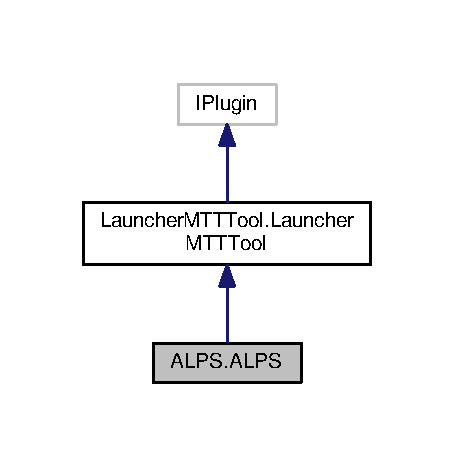
\includegraphics[width=218pt]{classALPS_1_1ALPS__inherit__graph}
\end{center}
\end{figure}


Collaboration diagram for A\-L\-P\-S.\-A\-L\-P\-S\-:
\nopagebreak
\begin{figure}[H]
\begin{center}
\leavevmode
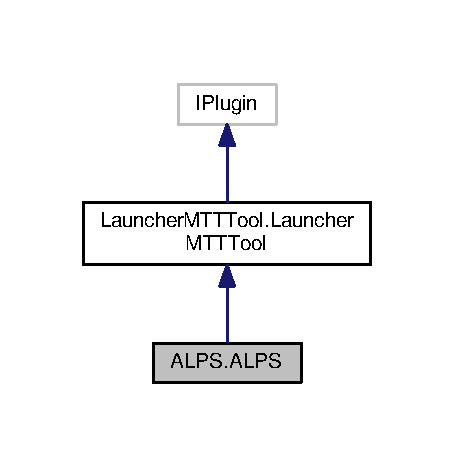
\includegraphics[width=218pt]{classALPS_1_1ALPS__coll__graph}
\end{center}
\end{figure}
\subsection*{Public Member Functions}
\begin{DoxyCompactItemize}
\item 
def \hyperlink{classALPS_1_1ALPS_a45417f6290435c66b3f3b7c4586915d9}{\-\_\-\-\_\-init\-\_\-\-\_\-}
\item 
def \hyperlink{classALPS_1_1ALPS_a3d507bd3feb505c8ed1b4e8f3729d636}{activate}
\item 
def \hyperlink{classALPS_1_1ALPS_aa1d63291a23bcca8ccbd44dc4d0fa6bf}{deactivate}
\item 
def \hyperlink{classALPS_1_1ALPS_a97e56ee7f5faaea26121d6ee0deeddab}{print\-\_\-name}
\item 
def \hyperlink{classALPS_1_1ALPS_a68c17d876ad850e44d40aa082b674f4e}{print\-\_\-options}
\item 
def \hyperlink{classALPS_1_1ALPS_af4b8efc64ea3abc5fb21fb93bfe052ff}{execute}
\end{DoxyCompactItemize}
\subsection*{Public Attributes}
\begin{DoxyCompactItemize}
\item 
\hyperlink{classALPS_1_1ALPS_a24dfa9b508f507c4cb6148f10a081555}{options}
\item 
\hyperlink{classALPS_1_1ALPS_ac371dce53e8c120f7031259025562bdb}{allocated}
\item 
\hyperlink{classALPS_1_1ALPS_a839c4f84a46683221d51004c08345ff2}{test\-Def}
\item 
\hyperlink{classALPS_1_1ALPS_a64bae95ba692ef4df06f716692b50ee9}{cmds}
\end{DoxyCompactItemize}


\subsection{Detailed Description}


Definition at line 40 of file A\-L\-P\-S.\-py.



\subsection{Constructor \& Destructor Documentation}
\hypertarget{classALPS_1_1ALPS_a45417f6290435c66b3f3b7c4586915d9}{\index{A\-L\-P\-S\-::\-A\-L\-P\-S@{A\-L\-P\-S\-::\-A\-L\-P\-S}!\-\_\-\-\_\-init\-\_\-\-\_\-@{\-\_\-\-\_\-init\-\_\-\-\_\-}}
\index{\-\_\-\-\_\-init\-\_\-\-\_\-@{\-\_\-\-\_\-init\-\_\-\-\_\-}!ALPS::ALPS@{A\-L\-P\-S\-::\-A\-L\-P\-S}}
\subsubsection[{\-\_\-\-\_\-init\-\_\-\-\_\-}]{\setlength{\rightskip}{0pt plus 5cm}def A\-L\-P\-S.\-A\-L\-P\-S.\-\_\-\-\_\-init\-\_\-\-\_\- (
\begin{DoxyParamCaption}
\item[{}]{self}
\end{DoxyParamCaption}
)}}\label{classALPS_1_1ALPS_a45417f6290435c66b3f3b7c4586915d9}


Definition at line 42 of file A\-L\-P\-S.\-py.



\subsection{Member Function Documentation}
\hypertarget{classALPS_1_1ALPS_a3d507bd3feb505c8ed1b4e8f3729d636}{\index{A\-L\-P\-S\-::\-A\-L\-P\-S@{A\-L\-P\-S\-::\-A\-L\-P\-S}!activate@{activate}}
\index{activate@{activate}!ALPS::ALPS@{A\-L\-P\-S\-::\-A\-L\-P\-S}}
\subsubsection[{activate}]{\setlength{\rightskip}{0pt plus 5cm}def A\-L\-P\-S.\-A\-L\-P\-S.\-activate (
\begin{DoxyParamCaption}
\item[{}]{self}
\end{DoxyParamCaption}
)}}\label{classALPS_1_1ALPS_a3d507bd3feb505c8ed1b4e8f3729d636}


Definition at line 72 of file A\-L\-P\-S.\-py.

\hypertarget{classALPS_1_1ALPS_aa1d63291a23bcca8ccbd44dc4d0fa6bf}{\index{A\-L\-P\-S\-::\-A\-L\-P\-S@{A\-L\-P\-S\-::\-A\-L\-P\-S}!deactivate@{deactivate}}
\index{deactivate@{deactivate}!ALPS::ALPS@{A\-L\-P\-S\-::\-A\-L\-P\-S}}
\subsubsection[{deactivate}]{\setlength{\rightskip}{0pt plus 5cm}def A\-L\-P\-S.\-A\-L\-P\-S.\-deactivate (
\begin{DoxyParamCaption}
\item[{}]{self}
\end{DoxyParamCaption}
)}}\label{classALPS_1_1ALPS_aa1d63291a23bcca8ccbd44dc4d0fa6bf}


Definition at line 78 of file A\-L\-P\-S.\-py.

\hypertarget{classALPS_1_1ALPS_af4b8efc64ea3abc5fb21fb93bfe052ff}{\index{A\-L\-P\-S\-::\-A\-L\-P\-S@{A\-L\-P\-S\-::\-A\-L\-P\-S}!execute@{execute}}
\index{execute@{execute}!ALPS::ALPS@{A\-L\-P\-S\-::\-A\-L\-P\-S}}
\subsubsection[{execute}]{\setlength{\rightskip}{0pt plus 5cm}def A\-L\-P\-S.\-A\-L\-P\-S.\-execute (
\begin{DoxyParamCaption}
\item[{}]{self, }
\item[{}]{log, }
\item[{}]{keyvals, }
\item[{}]{test\-Def}
\end{DoxyParamCaption}
)}}\label{classALPS_1_1ALPS_af4b8efc64ea3abc5fb21fb93bfe052ff}


Definition at line 95 of file A\-L\-P\-S.\-py.

\hypertarget{classALPS_1_1ALPS_a97e56ee7f5faaea26121d6ee0deeddab}{\index{A\-L\-P\-S\-::\-A\-L\-P\-S@{A\-L\-P\-S\-::\-A\-L\-P\-S}!print\-\_\-name@{print\-\_\-name}}
\index{print\-\_\-name@{print\-\_\-name}!ALPS::ALPS@{A\-L\-P\-S\-::\-A\-L\-P\-S}}
\subsubsection[{print\-\_\-name}]{\setlength{\rightskip}{0pt plus 5cm}def A\-L\-P\-S.\-A\-L\-P\-S.\-print\-\_\-name (
\begin{DoxyParamCaption}
\item[{}]{self}
\end{DoxyParamCaption}
)}}\label{classALPS_1_1ALPS_a97e56ee7f5faaea26121d6ee0deeddab}


Definition at line 86 of file A\-L\-P\-S.\-py.

\hypertarget{classALPS_1_1ALPS_a68c17d876ad850e44d40aa082b674f4e}{\index{A\-L\-P\-S\-::\-A\-L\-P\-S@{A\-L\-P\-S\-::\-A\-L\-P\-S}!print\-\_\-options@{print\-\_\-options}}
\index{print\-\_\-options@{print\-\_\-options}!ALPS::ALPS@{A\-L\-P\-S\-::\-A\-L\-P\-S}}
\subsubsection[{print\-\_\-options}]{\setlength{\rightskip}{0pt plus 5cm}def A\-L\-P\-S.\-A\-L\-P\-S.\-print\-\_\-options (
\begin{DoxyParamCaption}
\item[{}]{self, }
\item[{}]{test\-Def, }
\item[{}]{prefix}
\end{DoxyParamCaption}
)}}\label{classALPS_1_1ALPS_a68c17d876ad850e44d40aa082b674f4e}


Definition at line 89 of file A\-L\-P\-S.\-py.



\subsection{Member Data Documentation}
\hypertarget{classALPS_1_1ALPS_ac371dce53e8c120f7031259025562bdb}{\index{A\-L\-P\-S\-::\-A\-L\-P\-S@{A\-L\-P\-S\-::\-A\-L\-P\-S}!allocated@{allocated}}
\index{allocated@{allocated}!ALPS::ALPS@{A\-L\-P\-S\-::\-A\-L\-P\-S}}
\subsubsection[{allocated}]{\setlength{\rightskip}{0pt plus 5cm}A\-L\-P\-S.\-A\-L\-P\-S.\-allocated}}\label{classALPS_1_1ALPS_ac371dce53e8c120f7031259025562bdb}


Definition at line 66 of file A\-L\-P\-S.\-py.

\hypertarget{classALPS_1_1ALPS_a64bae95ba692ef4df06f716692b50ee9}{\index{A\-L\-P\-S\-::\-A\-L\-P\-S@{A\-L\-P\-S\-::\-A\-L\-P\-S}!cmds@{cmds}}
\index{cmds@{cmds}!ALPS::ALPS@{A\-L\-P\-S\-::\-A\-L\-P\-S}}
\subsubsection[{cmds}]{\setlength{\rightskip}{0pt plus 5cm}A\-L\-P\-S.\-A\-L\-P\-S.\-cmds}}\label{classALPS_1_1ALPS_a64bae95ba692ef4df06f716692b50ee9}


Definition at line 68 of file A\-L\-P\-S.\-py.

\hypertarget{classALPS_1_1ALPS_a24dfa9b508f507c4cb6148f10a081555}{\index{A\-L\-P\-S\-::\-A\-L\-P\-S@{A\-L\-P\-S\-::\-A\-L\-P\-S}!options@{options}}
\index{options@{options}!ALPS::ALPS@{A\-L\-P\-S\-::\-A\-L\-P\-S}}
\subsubsection[{options}]{\setlength{\rightskip}{0pt plus 5cm}A\-L\-P\-S.\-A\-L\-P\-S.\-options}}\label{classALPS_1_1ALPS_a24dfa9b508f507c4cb6148f10a081555}


Definition at line 45 of file A\-L\-P\-S.\-py.

\hypertarget{classALPS_1_1ALPS_a839c4f84a46683221d51004c08345ff2}{\index{A\-L\-P\-S\-::\-A\-L\-P\-S@{A\-L\-P\-S\-::\-A\-L\-P\-S}!test\-Def@{test\-Def}}
\index{test\-Def@{test\-Def}!ALPS::ALPS@{A\-L\-P\-S\-::\-A\-L\-P\-S}}
\subsubsection[{test\-Def}]{\setlength{\rightskip}{0pt plus 5cm}A\-L\-P\-S.\-A\-L\-P\-S.\-test\-Def}}\label{classALPS_1_1ALPS_a839c4f84a46683221d51004c08345ff2}


Definition at line 67 of file A\-L\-P\-S.\-py.



The documentation for this class was generated from the following file\-:\begin{DoxyCompactItemize}
\item 
/home/travis/build/open-\/mpi/mtt/pylib/\-Tools/\-Launcher/\hyperlink{ALPS_8py}{A\-L\-P\-S.\-py}\end{DoxyCompactItemize}

\hypertarget{classAlreadyInstalled_1_1AlreadyInstalled}{\section{Already\-Installed.\-Already\-Installed Class Reference}
\label{classAlreadyInstalled_1_1AlreadyInstalled}\index{Already\-Installed.\-Already\-Installed@{Already\-Installed.\-Already\-Installed}}
}


Inheritance diagram for Already\-Installed.\-Already\-Installed\-:
\nopagebreak
\begin{figure}[H]
\begin{center}
\leavevmode
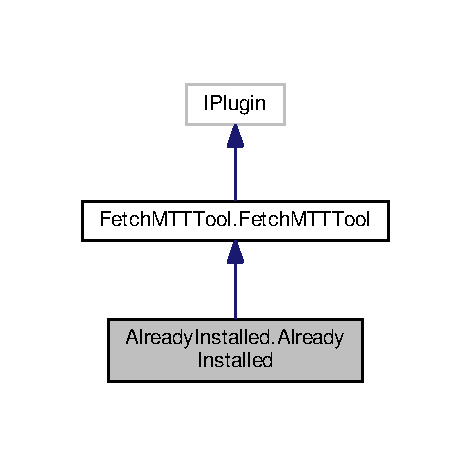
\includegraphics[width=226pt]{classAlreadyInstalled_1_1AlreadyInstalled__inherit__graph}
\end{center}
\end{figure}


Collaboration diagram for Already\-Installed.\-Already\-Installed\-:
\nopagebreak
\begin{figure}[H]
\begin{center}
\leavevmode
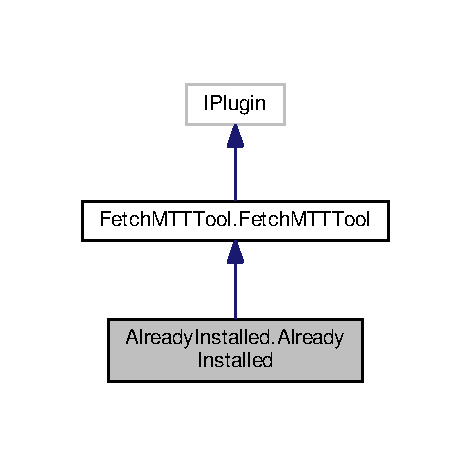
\includegraphics[width=226pt]{classAlreadyInstalled_1_1AlreadyInstalled__coll__graph}
\end{center}
\end{figure}
\subsection*{Public Member Functions}
\begin{DoxyCompactItemize}
\item 
def \hyperlink{classAlreadyInstalled_1_1AlreadyInstalled_ad412a2ca55660bde9d102ffffea5685f}{\-\_\-\-\_\-init\-\_\-\-\_\-}
\item 
def \hyperlink{classAlreadyInstalled_1_1AlreadyInstalled_aa69327b411af4bc2cd43f2bbf07cfe56}{activate}
\item 
def \hyperlink{classAlreadyInstalled_1_1AlreadyInstalled_a895aa66471ba8b5d4f67f8d17df5131c}{deactivate}
\item 
def \hyperlink{classAlreadyInstalled_1_1AlreadyInstalled_a63ce43492cf6c53f23a19a444109bfa8}{print\-\_\-name}
\item 
def \hyperlink{classAlreadyInstalled_1_1AlreadyInstalled_a8061d145324dbf058b17bc16579e9d5f}{print\-\_\-options}
\item 
def \hyperlink{classAlreadyInstalled_1_1AlreadyInstalled_af1afb26d21ce30a80e68c834245baeda}{execute}
\end{DoxyCompactItemize}
\subsection*{Public Attributes}
\begin{DoxyCompactItemize}
\item 
\hyperlink{classAlreadyInstalled_1_1AlreadyInstalled_af9247ff7a3b5dab409644868b7cc34e3}{options}
\end{DoxyCompactItemize}


\subsection{Detailed Description}


Definition at line 24 of file Already\-Installed.\-py.



\subsection{Constructor \& Destructor Documentation}
\hypertarget{classAlreadyInstalled_1_1AlreadyInstalled_ad412a2ca55660bde9d102ffffea5685f}{\index{Already\-Installed\-::\-Already\-Installed@{Already\-Installed\-::\-Already\-Installed}!\-\_\-\-\_\-init\-\_\-\-\_\-@{\-\_\-\-\_\-init\-\_\-\-\_\-}}
\index{\-\_\-\-\_\-init\-\_\-\-\_\-@{\-\_\-\-\_\-init\-\_\-\-\_\-}!AlreadyInstalled::AlreadyInstalled@{Already\-Installed\-::\-Already\-Installed}}
\subsubsection[{\-\_\-\-\_\-init\-\_\-\-\_\-}]{\setlength{\rightskip}{0pt plus 5cm}def Already\-Installed.\-Already\-Installed.\-\_\-\-\_\-init\-\_\-\-\_\- (
\begin{DoxyParamCaption}
\item[{}]{self}
\end{DoxyParamCaption}
)}}\label{classAlreadyInstalled_1_1AlreadyInstalled_ad412a2ca55660bde9d102ffffea5685f}


Definition at line 26 of file Already\-Installed.\-py.



\subsection{Member Function Documentation}
\hypertarget{classAlreadyInstalled_1_1AlreadyInstalled_aa69327b411af4bc2cd43f2bbf07cfe56}{\index{Already\-Installed\-::\-Already\-Installed@{Already\-Installed\-::\-Already\-Installed}!activate@{activate}}
\index{activate@{activate}!AlreadyInstalled::AlreadyInstalled@{Already\-Installed\-::\-Already\-Installed}}
\subsubsection[{activate}]{\setlength{\rightskip}{0pt plus 5cm}def Already\-Installed.\-Already\-Installed.\-activate (
\begin{DoxyParamCaption}
\item[{}]{self}
\end{DoxyParamCaption}
)}}\label{classAlreadyInstalled_1_1AlreadyInstalled_aa69327b411af4bc2cd43f2bbf07cfe56}


Definition at line 34 of file Already\-Installed.\-py.

\hypertarget{classAlreadyInstalled_1_1AlreadyInstalled_a895aa66471ba8b5d4f67f8d17df5131c}{\index{Already\-Installed\-::\-Already\-Installed@{Already\-Installed\-::\-Already\-Installed}!deactivate@{deactivate}}
\index{deactivate@{deactivate}!AlreadyInstalled::AlreadyInstalled@{Already\-Installed\-::\-Already\-Installed}}
\subsubsection[{deactivate}]{\setlength{\rightskip}{0pt plus 5cm}def Already\-Installed.\-Already\-Installed.\-deactivate (
\begin{DoxyParamCaption}
\item[{}]{self}
\end{DoxyParamCaption}
)}}\label{classAlreadyInstalled_1_1AlreadyInstalled_a895aa66471ba8b5d4f67f8d17df5131c}


Definition at line 40 of file Already\-Installed.\-py.

\hypertarget{classAlreadyInstalled_1_1AlreadyInstalled_af1afb26d21ce30a80e68c834245baeda}{\index{Already\-Installed\-::\-Already\-Installed@{Already\-Installed\-::\-Already\-Installed}!execute@{execute}}
\index{execute@{execute}!AlreadyInstalled::AlreadyInstalled@{Already\-Installed\-::\-Already\-Installed}}
\subsubsection[{execute}]{\setlength{\rightskip}{0pt plus 5cm}def Already\-Installed.\-Already\-Installed.\-execute (
\begin{DoxyParamCaption}
\item[{}]{self, }
\item[{}]{log, }
\item[{}]{keyvals, }
\item[{}]{test\-Def}
\end{DoxyParamCaption}
)}}\label{classAlreadyInstalled_1_1AlreadyInstalled_af1afb26d21ce30a80e68c834245baeda}


Definition at line 53 of file Already\-Installed.\-py.

\hypertarget{classAlreadyInstalled_1_1AlreadyInstalled_a63ce43492cf6c53f23a19a444109bfa8}{\index{Already\-Installed\-::\-Already\-Installed@{Already\-Installed\-::\-Already\-Installed}!print\-\_\-name@{print\-\_\-name}}
\index{print\-\_\-name@{print\-\_\-name}!AlreadyInstalled::AlreadyInstalled@{Already\-Installed\-::\-Already\-Installed}}
\subsubsection[{print\-\_\-name}]{\setlength{\rightskip}{0pt plus 5cm}def Already\-Installed.\-Already\-Installed.\-print\-\_\-name (
\begin{DoxyParamCaption}
\item[{}]{self}
\end{DoxyParamCaption}
)}}\label{classAlreadyInstalled_1_1AlreadyInstalled_a63ce43492cf6c53f23a19a444109bfa8}


Definition at line 44 of file Already\-Installed.\-py.

\hypertarget{classAlreadyInstalled_1_1AlreadyInstalled_a8061d145324dbf058b17bc16579e9d5f}{\index{Already\-Installed\-::\-Already\-Installed@{Already\-Installed\-::\-Already\-Installed}!print\-\_\-options@{print\-\_\-options}}
\index{print\-\_\-options@{print\-\_\-options}!AlreadyInstalled::AlreadyInstalled@{Already\-Installed\-::\-Already\-Installed}}
\subsubsection[{print\-\_\-options}]{\setlength{\rightskip}{0pt plus 5cm}def Already\-Installed.\-Already\-Installed.\-print\-\_\-options (
\begin{DoxyParamCaption}
\item[{}]{self, }
\item[{}]{test\-Def, }
\item[{}]{prefix}
\end{DoxyParamCaption}
)}}\label{classAlreadyInstalled_1_1AlreadyInstalled_a8061d145324dbf058b17bc16579e9d5f}


Definition at line 47 of file Already\-Installed.\-py.



\subsection{Member Data Documentation}
\hypertarget{classAlreadyInstalled_1_1AlreadyInstalled_af9247ff7a3b5dab409644868b7cc34e3}{\index{Already\-Installed\-::\-Already\-Installed@{Already\-Installed\-::\-Already\-Installed}!options@{options}}
\index{options@{options}!AlreadyInstalled::AlreadyInstalled@{Already\-Installed\-::\-Already\-Installed}}
\subsubsection[{options}]{\setlength{\rightskip}{0pt plus 5cm}Already\-Installed.\-Already\-Installed.\-options}}\label{classAlreadyInstalled_1_1AlreadyInstalled_af9247ff7a3b5dab409644868b7cc34e3}


Definition at line 29 of file Already\-Installed.\-py.



The documentation for this class was generated from the following file\-:\begin{DoxyCompactItemize}
\item 
/home/travis/build/open-\/mpi/mtt/pylib/\-Tools/\-Fetch/\hyperlink{AlreadyInstalled_8py}{Already\-Installed.\-py}\end{DoxyCompactItemize}

\hypertarget{classAutotools_1_1Autotools}{\section{Autotools.\-Autotools Class Reference}
\label{classAutotools_1_1Autotools}\index{Autotools.\-Autotools@{Autotools.\-Autotools}}
}


Inheritance diagram for Autotools.\-Autotools\-:
\nopagebreak
\begin{figure}[H]
\begin{center}
\leavevmode
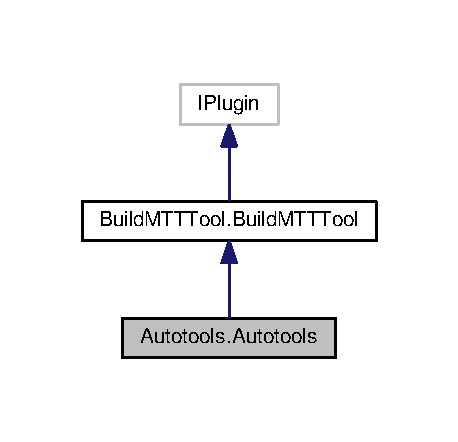
\includegraphics[width=220pt]{classAutotools_1_1Autotools__inherit__graph}
\end{center}
\end{figure}


Collaboration diagram for Autotools.\-Autotools\-:
\nopagebreak
\begin{figure}[H]
\begin{center}
\leavevmode
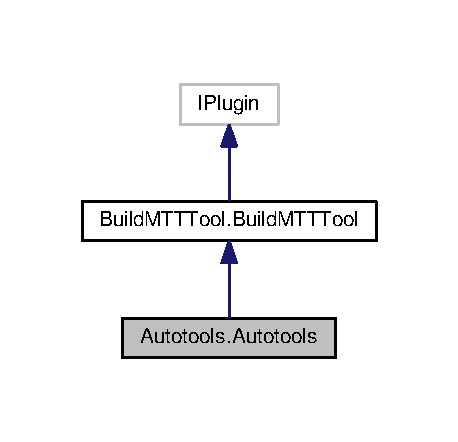
\includegraphics[width=220pt]{classAutotools_1_1Autotools__coll__graph}
\end{center}
\end{figure}
\subsection*{Public Member Functions}
\begin{DoxyCompactItemize}
\item 
def \hyperlink{classAutotools_1_1Autotools_a5b5ac092ad7f4bc45bf785633c8be95a}{\-\_\-\-\_\-init\-\_\-\-\_\-}
\item 
def \hyperlink{classAutotools_1_1Autotools_a202b0e727db575d20a381cd039dd3597}{activate}
\item 
def \hyperlink{classAutotools_1_1Autotools_a74513a2f4135b506e66c047559f9571e}{deactivate}
\item 
def \hyperlink{classAutotools_1_1Autotools_a0873459245ef2255a5a7386957fa592e}{print\-\_\-name}
\item 
def \hyperlink{classAutotools_1_1Autotools_a41481e9f2a7e7fce32f51cc8feb909fd}{print\-\_\-options}
\item 
def \hyperlink{classAutotools_1_1Autotools_a5ae85e70e9e6252f4be23ef60624f633}{execute}
\end{DoxyCompactItemize}
\subsection*{Public Attributes}
\begin{DoxyCompactItemize}
\item 
\hyperlink{classAutotools_1_1Autotools_a6bbb714a91bc8b6fe749326772b073b3}{activated}
\item 
\hyperlink{classAutotools_1_1Autotools_a8b348e19f0a7104bde9c43c3a6ed695d}{options}
\item 
\hyperlink{classAutotools_1_1Autotools_aee37d9789ea22ee310ebc357cd721b7f}{exclude}
\end{DoxyCompactItemize}


\subsection{Detailed Description}


Definition at line 36 of file Autotools.\-py.



\subsection{Constructor \& Destructor Documentation}
\hypertarget{classAutotools_1_1Autotools_a5b5ac092ad7f4bc45bf785633c8be95a}{\index{Autotools\-::\-Autotools@{Autotools\-::\-Autotools}!\-\_\-\-\_\-init\-\_\-\-\_\-@{\-\_\-\-\_\-init\-\_\-\-\_\-}}
\index{\-\_\-\-\_\-init\-\_\-\-\_\-@{\-\_\-\-\_\-init\-\_\-\-\_\-}!Autotools::Autotools@{Autotools\-::\-Autotools}}
\subsubsection[{\-\_\-\-\_\-init\-\_\-\-\_\-}]{\setlength{\rightskip}{0pt plus 5cm}def Autotools.\-Autotools.\-\_\-\-\_\-init\-\_\-\-\_\- (
\begin{DoxyParamCaption}
\item[{}]{self}
\end{DoxyParamCaption}
)}}\label{classAutotools_1_1Autotools_a5b5ac092ad7f4bc45bf785633c8be95a}


Definition at line 37 of file Autotools.\-py.



\subsection{Member Function Documentation}
\hypertarget{classAutotools_1_1Autotools_a202b0e727db575d20a381cd039dd3597}{\index{Autotools\-::\-Autotools@{Autotools\-::\-Autotools}!activate@{activate}}
\index{activate@{activate}!Autotools::Autotools@{Autotools\-::\-Autotools}}
\subsubsection[{activate}]{\setlength{\rightskip}{0pt plus 5cm}def Autotools.\-Autotools.\-activate (
\begin{DoxyParamCaption}
\item[{}]{self}
\end{DoxyParamCaption}
)}}\label{classAutotools_1_1Autotools_a202b0e727db575d20a381cd039dd3597}


Definition at line 55 of file Autotools.\-py.

\hypertarget{classAutotools_1_1Autotools_a74513a2f4135b506e66c047559f9571e}{\index{Autotools\-::\-Autotools@{Autotools\-::\-Autotools}!deactivate@{deactivate}}
\index{deactivate@{deactivate}!Autotools::Autotools@{Autotools\-::\-Autotools}}
\subsubsection[{deactivate}]{\setlength{\rightskip}{0pt plus 5cm}def Autotools.\-Autotools.\-deactivate (
\begin{DoxyParamCaption}
\item[{}]{self}
\end{DoxyParamCaption}
)}}\label{classAutotools_1_1Autotools_a74513a2f4135b506e66c047559f9571e}


Definition at line 62 of file Autotools.\-py.

\hypertarget{classAutotools_1_1Autotools_a5ae85e70e9e6252f4be23ef60624f633}{\index{Autotools\-::\-Autotools@{Autotools\-::\-Autotools}!execute@{execute}}
\index{execute@{execute}!Autotools::Autotools@{Autotools\-::\-Autotools}}
\subsubsection[{execute}]{\setlength{\rightskip}{0pt plus 5cm}def Autotools.\-Autotools.\-execute (
\begin{DoxyParamCaption}
\item[{}]{self, }
\item[{}]{log, }
\item[{}]{keyvals, }
\item[{}]{test\-Def}
\end{DoxyParamCaption}
)}}\label{classAutotools_1_1Autotools_a5ae85e70e9e6252f4be23ef60624f633}


Definition at line 77 of file Autotools.\-py.

\hypertarget{classAutotools_1_1Autotools_a0873459245ef2255a5a7386957fa592e}{\index{Autotools\-::\-Autotools@{Autotools\-::\-Autotools}!print\-\_\-name@{print\-\_\-name}}
\index{print\-\_\-name@{print\-\_\-name}!Autotools::Autotools@{Autotools\-::\-Autotools}}
\subsubsection[{print\-\_\-name}]{\setlength{\rightskip}{0pt plus 5cm}def Autotools.\-Autotools.\-print\-\_\-name (
\begin{DoxyParamCaption}
\item[{}]{self}
\end{DoxyParamCaption}
)}}\label{classAutotools_1_1Autotools_a0873459245ef2255a5a7386957fa592e}


Definition at line 68 of file Autotools.\-py.

\hypertarget{classAutotools_1_1Autotools_a41481e9f2a7e7fce32f51cc8feb909fd}{\index{Autotools\-::\-Autotools@{Autotools\-::\-Autotools}!print\-\_\-options@{print\-\_\-options}}
\index{print\-\_\-options@{print\-\_\-options}!Autotools::Autotools@{Autotools\-::\-Autotools}}
\subsubsection[{print\-\_\-options}]{\setlength{\rightskip}{0pt plus 5cm}def Autotools.\-Autotools.\-print\-\_\-options (
\begin{DoxyParamCaption}
\item[{}]{self, }
\item[{}]{test\-Def, }
\item[{}]{prefix}
\end{DoxyParamCaption}
)}}\label{classAutotools_1_1Autotools_a41481e9f2a7e7fce32f51cc8feb909fd}


Definition at line 71 of file Autotools.\-py.



\subsection{Member Data Documentation}
\hypertarget{classAutotools_1_1Autotools_a6bbb714a91bc8b6fe749326772b073b3}{\index{Autotools\-::\-Autotools@{Autotools\-::\-Autotools}!activated@{activated}}
\index{activated@{activated}!Autotools::Autotools@{Autotools\-::\-Autotools}}
\subsubsection[{activated}]{\setlength{\rightskip}{0pt plus 5cm}Autotools.\-Autotools.\-activated}}\label{classAutotools_1_1Autotools_a6bbb714a91bc8b6fe749326772b073b3}


Definition at line 39 of file Autotools.\-py.

\hypertarget{classAutotools_1_1Autotools_aee37d9789ea22ee310ebc357cd721b7f}{\index{Autotools\-::\-Autotools@{Autotools\-::\-Autotools}!exclude@{exclude}}
\index{exclude@{exclude}!Autotools::Autotools@{Autotools\-::\-Autotools}}
\subsubsection[{exclude}]{\setlength{\rightskip}{0pt plus 5cm}Autotools.\-Autotools.\-exclude}}\label{classAutotools_1_1Autotools_aee37d9789ea22ee310ebc357cd721b7f}


Definition at line 52 of file Autotools.\-py.

\hypertarget{classAutotools_1_1Autotools_a8b348e19f0a7104bde9c43c3a6ed695d}{\index{Autotools\-::\-Autotools@{Autotools\-::\-Autotools}!options@{options}}
\index{options@{options}!Autotools::Autotools@{Autotools\-::\-Autotools}}
\subsubsection[{options}]{\setlength{\rightskip}{0pt plus 5cm}Autotools.\-Autotools.\-options}}\label{classAutotools_1_1Autotools_a8b348e19f0a7104bde9c43c3a6ed695d}


Definition at line 40 of file Autotools.\-py.



The documentation for this class was generated from the following file\-:\begin{DoxyCompactItemize}
\item 
/home/travis/build/open-\/mpi/mtt/pylib/\-Tools/\-Build/\hyperlink{Autotools_8py}{Autotools.\-py}\end{DoxyCompactItemize}

\hypertarget{classBaseMTTUtility_1_1BaseMTTUtility}{\section{Base\-M\-T\-T\-Utility.\-Base\-M\-T\-T\-Utility Class Reference}
\label{classBaseMTTUtility_1_1BaseMTTUtility}\index{Base\-M\-T\-T\-Utility.\-Base\-M\-T\-T\-Utility@{Base\-M\-T\-T\-Utility.\-Base\-M\-T\-T\-Utility}}
}


Inheritance diagram for Base\-M\-T\-T\-Utility.\-Base\-M\-T\-T\-Utility\-:
\nopagebreak
\begin{figure}[H]
\begin{center}
\leavevmode
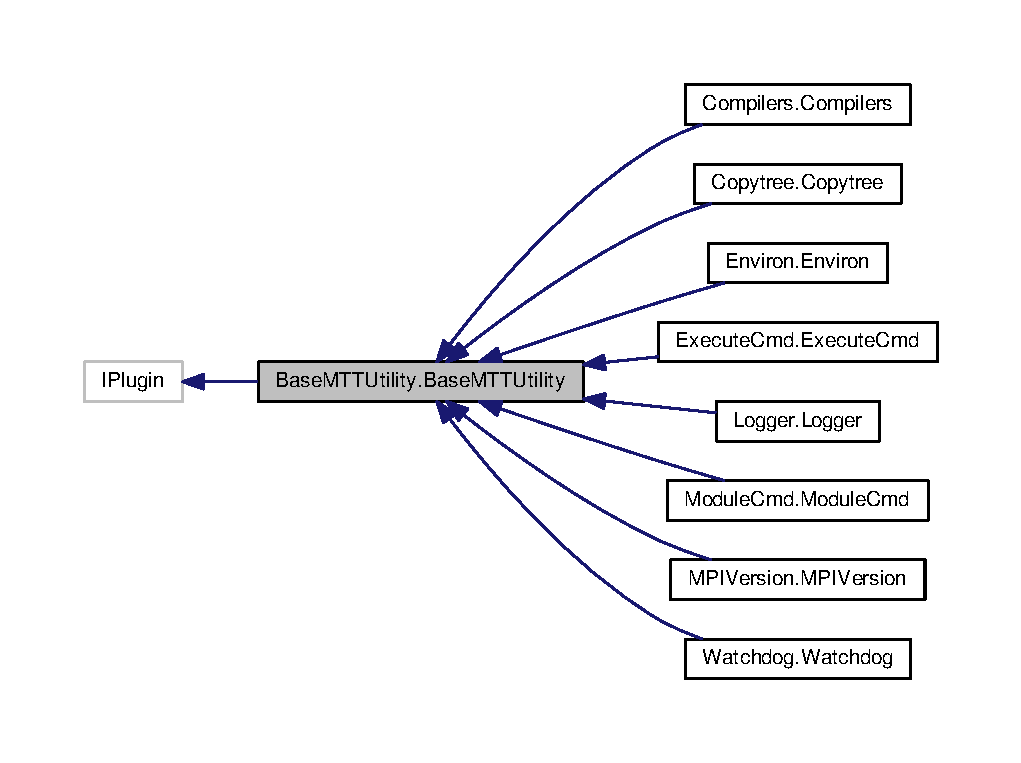
\includegraphics[width=350pt]{classBaseMTTUtility_1_1BaseMTTUtility__inherit__graph}
\end{center}
\end{figure}


Collaboration diagram for Base\-M\-T\-T\-Utility.\-Base\-M\-T\-T\-Utility\-:
\nopagebreak
\begin{figure}[H]
\begin{center}
\leavevmode
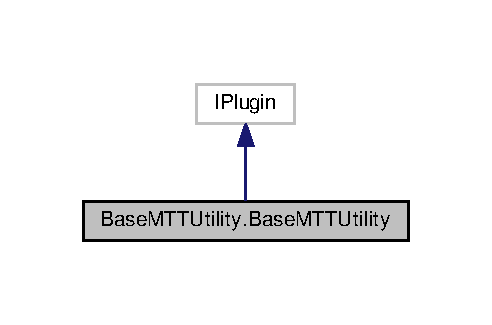
\includegraphics[width=236pt]{classBaseMTTUtility_1_1BaseMTTUtility__coll__graph}
\end{center}
\end{figure}
\subsection*{Public Member Functions}
\begin{DoxyCompactItemize}
\item 
def \hyperlink{classBaseMTTUtility_1_1BaseMTTUtility_acc17cee13f814473c5cea32a8e2eebeb}{\-\_\-\-\_\-init\-\_\-\-\_\-}
\item 
def \hyperlink{classBaseMTTUtility_1_1BaseMTTUtility_a65cd8c577d1fea0bf1edc05969fbe31e}{print\-\_\-name}
\end{DoxyCompactItemize}


\subsection{Detailed Description}


Definition at line 14 of file Base\-M\-T\-T\-Utility.\-py.



\subsection{Constructor \& Destructor Documentation}
\hypertarget{classBaseMTTUtility_1_1BaseMTTUtility_acc17cee13f814473c5cea32a8e2eebeb}{\index{Base\-M\-T\-T\-Utility\-::\-Base\-M\-T\-T\-Utility@{Base\-M\-T\-T\-Utility\-::\-Base\-M\-T\-T\-Utility}!\-\_\-\-\_\-init\-\_\-\-\_\-@{\-\_\-\-\_\-init\-\_\-\-\_\-}}
\index{\-\_\-\-\_\-init\-\_\-\-\_\-@{\-\_\-\-\_\-init\-\_\-\-\_\-}!BaseMTTUtility::BaseMTTUtility@{Base\-M\-T\-T\-Utility\-::\-Base\-M\-T\-T\-Utility}}
\subsubsection[{\-\_\-\-\_\-init\-\_\-\-\_\-}]{\setlength{\rightskip}{0pt plus 5cm}def Base\-M\-T\-T\-Utility.\-Base\-M\-T\-T\-Utility.\-\_\-\-\_\-init\-\_\-\-\_\- (
\begin{DoxyParamCaption}
\item[{}]{self}
\end{DoxyParamCaption}
)}}\label{classBaseMTTUtility_1_1BaseMTTUtility_acc17cee13f814473c5cea32a8e2eebeb}


Definition at line 15 of file Base\-M\-T\-T\-Utility.\-py.



\subsection{Member Function Documentation}
\hypertarget{classBaseMTTUtility_1_1BaseMTTUtility_a65cd8c577d1fea0bf1edc05969fbe31e}{\index{Base\-M\-T\-T\-Utility\-::\-Base\-M\-T\-T\-Utility@{Base\-M\-T\-T\-Utility\-::\-Base\-M\-T\-T\-Utility}!print\-\_\-name@{print\-\_\-name}}
\index{print\-\_\-name@{print\-\_\-name}!BaseMTTUtility::BaseMTTUtility@{Base\-M\-T\-T\-Utility\-::\-Base\-M\-T\-T\-Utility}}
\subsubsection[{print\-\_\-name}]{\setlength{\rightskip}{0pt plus 5cm}def Base\-M\-T\-T\-Utility.\-Base\-M\-T\-T\-Utility.\-print\-\_\-name (
\begin{DoxyParamCaption}
\item[{}]{self}
\end{DoxyParamCaption}
)}}\label{classBaseMTTUtility_1_1BaseMTTUtility_a65cd8c577d1fea0bf1edc05969fbe31e}


Definition at line 19 of file Base\-M\-T\-T\-Utility.\-py.



The documentation for this class was generated from the following file\-:\begin{DoxyCompactItemize}
\item 
/home/travis/build/open-\/mpi/mtt/pylib/\-Utilities/\hyperlink{BaseMTTUtility_8py}{Base\-M\-T\-T\-Utility.\-py}\end{DoxyCompactItemize}

\hypertarget{classBIOSMTTStage_1_1BIOSMTTStage}{\section{B\-I\-O\-S\-M\-T\-T\-Stage.\-B\-I\-O\-S\-M\-T\-T\-Stage Class Reference}
\label{classBIOSMTTStage_1_1BIOSMTTStage}\index{B\-I\-O\-S\-M\-T\-T\-Stage.\-B\-I\-O\-S\-M\-T\-T\-Stage@{B\-I\-O\-S\-M\-T\-T\-Stage.\-B\-I\-O\-S\-M\-T\-T\-Stage}}
}


Inheritance diagram for B\-I\-O\-S\-M\-T\-T\-Stage.\-B\-I\-O\-S\-M\-T\-T\-Stage\-:
\nopagebreak
\begin{figure}[H]
\begin{center}
\leavevmode
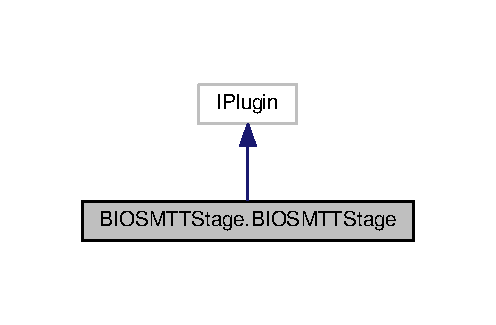
\includegraphics[width=238pt]{classBIOSMTTStage_1_1BIOSMTTStage__inherit__graph}
\end{center}
\end{figure}


Collaboration diagram for B\-I\-O\-S\-M\-T\-T\-Stage.\-B\-I\-O\-S\-M\-T\-T\-Stage\-:
\nopagebreak
\begin{figure}[H]
\begin{center}
\leavevmode
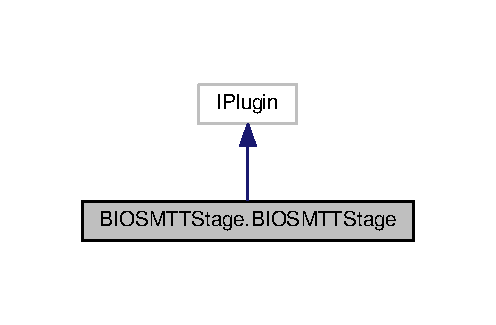
\includegraphics[width=238pt]{classBIOSMTTStage_1_1BIOSMTTStage__coll__graph}
\end{center}
\end{figure}
\subsection*{Public Member Functions}
\begin{DoxyCompactItemize}
\item 
def \hyperlink{classBIOSMTTStage_1_1BIOSMTTStage_aa5f27b6db5d3b10cbd5d6e47de378e58}{\-\_\-\-\_\-init\-\_\-\-\_\-}
\item 
def \hyperlink{classBIOSMTTStage_1_1BIOSMTTStage_a4e5d3ca4920bd6825cdda7259fa85d52}{print\-\_\-name}
\item 
def \hyperlink{classBIOSMTTStage_1_1BIOSMTTStage_ae46a6ddd03499b39c15d164ea3643e48}{ordering}
\end{DoxyCompactItemize}


\subsection{Detailed Description}


Definition at line 19 of file B\-I\-O\-S\-M\-T\-T\-Stage.\-py.



\subsection{Constructor \& Destructor Documentation}
\hypertarget{classBIOSMTTStage_1_1BIOSMTTStage_aa5f27b6db5d3b10cbd5d6e47de378e58}{\index{B\-I\-O\-S\-M\-T\-T\-Stage\-::\-B\-I\-O\-S\-M\-T\-T\-Stage@{B\-I\-O\-S\-M\-T\-T\-Stage\-::\-B\-I\-O\-S\-M\-T\-T\-Stage}!\-\_\-\-\_\-init\-\_\-\-\_\-@{\-\_\-\-\_\-init\-\_\-\-\_\-}}
\index{\-\_\-\-\_\-init\-\_\-\-\_\-@{\-\_\-\-\_\-init\-\_\-\-\_\-}!BIOSMTTStage::BIOSMTTStage@{B\-I\-O\-S\-M\-T\-T\-Stage\-::\-B\-I\-O\-S\-M\-T\-T\-Stage}}
\subsubsection[{\-\_\-\-\_\-init\-\_\-\-\_\-}]{\setlength{\rightskip}{0pt plus 5cm}def B\-I\-O\-S\-M\-T\-T\-Stage.\-B\-I\-O\-S\-M\-T\-T\-Stage.\-\_\-\-\_\-init\-\_\-\-\_\- (
\begin{DoxyParamCaption}
\item[{}]{self}
\end{DoxyParamCaption}
)}}\label{classBIOSMTTStage_1_1BIOSMTTStage_aa5f27b6db5d3b10cbd5d6e47de378e58}


Definition at line 20 of file B\-I\-O\-S\-M\-T\-T\-Stage.\-py.



\subsection{Member Function Documentation}
\hypertarget{classBIOSMTTStage_1_1BIOSMTTStage_ae46a6ddd03499b39c15d164ea3643e48}{\index{B\-I\-O\-S\-M\-T\-T\-Stage\-::\-B\-I\-O\-S\-M\-T\-T\-Stage@{B\-I\-O\-S\-M\-T\-T\-Stage\-::\-B\-I\-O\-S\-M\-T\-T\-Stage}!ordering@{ordering}}
\index{ordering@{ordering}!BIOSMTTStage::BIOSMTTStage@{B\-I\-O\-S\-M\-T\-T\-Stage\-::\-B\-I\-O\-S\-M\-T\-T\-Stage}}
\subsubsection[{ordering}]{\setlength{\rightskip}{0pt plus 5cm}def B\-I\-O\-S\-M\-T\-T\-Stage.\-B\-I\-O\-S\-M\-T\-T\-Stage.\-ordering (
\begin{DoxyParamCaption}
\item[{}]{self}
\end{DoxyParamCaption}
)}}\label{classBIOSMTTStage_1_1BIOSMTTStage_ae46a6ddd03499b39c15d164ea3643e48}


Definition at line 26 of file B\-I\-O\-S\-M\-T\-T\-Stage.\-py.

\hypertarget{classBIOSMTTStage_1_1BIOSMTTStage_a4e5d3ca4920bd6825cdda7259fa85d52}{\index{B\-I\-O\-S\-M\-T\-T\-Stage\-::\-B\-I\-O\-S\-M\-T\-T\-Stage@{B\-I\-O\-S\-M\-T\-T\-Stage\-::\-B\-I\-O\-S\-M\-T\-T\-Stage}!print\-\_\-name@{print\-\_\-name}}
\index{print\-\_\-name@{print\-\_\-name}!BIOSMTTStage::BIOSMTTStage@{B\-I\-O\-S\-M\-T\-T\-Stage\-::\-B\-I\-O\-S\-M\-T\-T\-Stage}}
\subsubsection[{print\-\_\-name}]{\setlength{\rightskip}{0pt plus 5cm}def B\-I\-O\-S\-M\-T\-T\-Stage.\-B\-I\-O\-S\-M\-T\-T\-Stage.\-print\-\_\-name (
\begin{DoxyParamCaption}
\item[{}]{self}
\end{DoxyParamCaption}
)}}\label{classBIOSMTTStage_1_1BIOSMTTStage_a4e5d3ca4920bd6825cdda7259fa85d52}


Definition at line 23 of file B\-I\-O\-S\-M\-T\-T\-Stage.\-py.



The documentation for this class was generated from the following file\-:\begin{DoxyCompactItemize}
\item 
/home/travis/build/open-\/mpi/mtt/pylib/\-Stages/\-B\-I\-O\-S/\hyperlink{BIOSMTTStage_8py}{B\-I\-O\-S\-M\-T\-T\-Stage.\-py}\end{DoxyCompactItemize}

\hypertarget{classBuildMTTTool_1_1BuildMTTTool}{\section{Build\-M\-T\-T\-Tool.\-Build\-M\-T\-T\-Tool Class Reference}
\label{classBuildMTTTool_1_1BuildMTTTool}\index{Build\-M\-T\-T\-Tool.\-Build\-M\-T\-T\-Tool@{Build\-M\-T\-T\-Tool.\-Build\-M\-T\-T\-Tool}}
}


Inheritance diagram for Build\-M\-T\-T\-Tool.\-Build\-M\-T\-T\-Tool\-:
\nopagebreak
\begin{figure}[H]
\begin{center}
\leavevmode
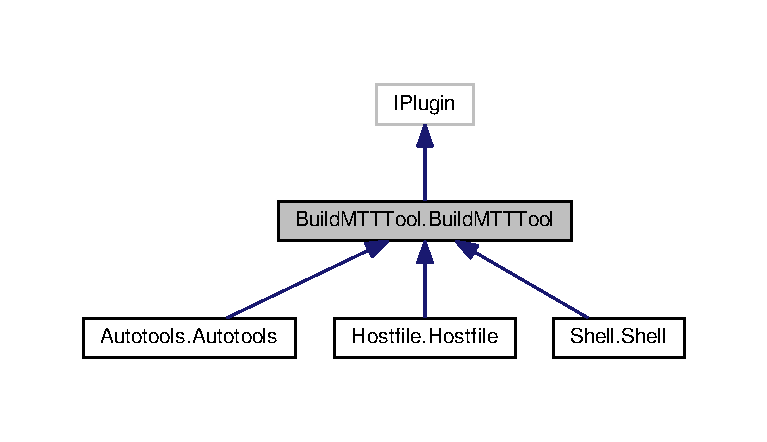
\includegraphics[width=350pt]{classBuildMTTTool_1_1BuildMTTTool__inherit__graph}
\end{center}
\end{figure}


Collaboration diagram for Build\-M\-T\-T\-Tool.\-Build\-M\-T\-T\-Tool\-:
\nopagebreak
\begin{figure}[H]
\begin{center}
\leavevmode
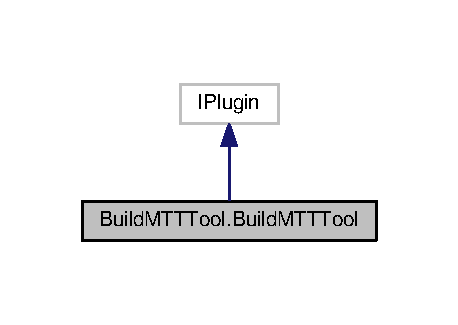
\includegraphics[width=220pt]{classBuildMTTTool_1_1BuildMTTTool__coll__graph}
\end{center}
\end{figure}
\subsection*{Public Member Functions}
\begin{DoxyCompactItemize}
\item 
def \hyperlink{classBuildMTTTool_1_1BuildMTTTool_a5665b0ed7a6ef42181601533cdbe74be}{\-\_\-\-\_\-init\-\_\-\-\_\-}
\item 
def \hyperlink{classBuildMTTTool_1_1BuildMTTTool_afbb7e8957f4c8c43e2937489173de162}{print\-\_\-name}
\end{DoxyCompactItemize}


\subsection{Detailed Description}


Definition at line 19 of file Build\-M\-T\-T\-Tool.\-py.



\subsection{Constructor \& Destructor Documentation}
\hypertarget{classBuildMTTTool_1_1BuildMTTTool_a5665b0ed7a6ef42181601533cdbe74be}{\index{Build\-M\-T\-T\-Tool\-::\-Build\-M\-T\-T\-Tool@{Build\-M\-T\-T\-Tool\-::\-Build\-M\-T\-T\-Tool}!\-\_\-\-\_\-init\-\_\-\-\_\-@{\-\_\-\-\_\-init\-\_\-\-\_\-}}
\index{\-\_\-\-\_\-init\-\_\-\-\_\-@{\-\_\-\-\_\-init\-\_\-\-\_\-}!BuildMTTTool::BuildMTTTool@{Build\-M\-T\-T\-Tool\-::\-Build\-M\-T\-T\-Tool}}
\subsubsection[{\-\_\-\-\_\-init\-\_\-\-\_\-}]{\setlength{\rightskip}{0pt plus 5cm}def Build\-M\-T\-T\-Tool.\-Build\-M\-T\-T\-Tool.\-\_\-\-\_\-init\-\_\-\-\_\- (
\begin{DoxyParamCaption}
\item[{}]{self}
\end{DoxyParamCaption}
)}}\label{classBuildMTTTool_1_1BuildMTTTool_a5665b0ed7a6ef42181601533cdbe74be}


Definition at line 20 of file Build\-M\-T\-T\-Tool.\-py.



\subsection{Member Function Documentation}
\hypertarget{classBuildMTTTool_1_1BuildMTTTool_afbb7e8957f4c8c43e2937489173de162}{\index{Build\-M\-T\-T\-Tool\-::\-Build\-M\-T\-T\-Tool@{Build\-M\-T\-T\-Tool\-::\-Build\-M\-T\-T\-Tool}!print\-\_\-name@{print\-\_\-name}}
\index{print\-\_\-name@{print\-\_\-name}!BuildMTTTool::BuildMTTTool@{Build\-M\-T\-T\-Tool\-::\-Build\-M\-T\-T\-Tool}}
\subsubsection[{print\-\_\-name}]{\setlength{\rightskip}{0pt plus 5cm}def Build\-M\-T\-T\-Tool.\-Build\-M\-T\-T\-Tool.\-print\-\_\-name (
\begin{DoxyParamCaption}
\item[{}]{self}
\end{DoxyParamCaption}
)}}\label{classBuildMTTTool_1_1BuildMTTTool_afbb7e8957f4c8c43e2937489173de162}


Definition at line 24 of file Build\-M\-T\-T\-Tool.\-py.



The documentation for this class was generated from the following file\-:\begin{DoxyCompactItemize}
\item 
/home/travis/build/open-\/mpi/mtt/pylib/\-Tools/\-Build/\hyperlink{BuildMTTTool_8py}{Build\-M\-T\-T\-Tool.\-py}\end{DoxyCompactItemize}

\hypertarget{classCheckProfile_1_1CheckProfile}{\section{Check\-Profile.\-Check\-Profile Class Reference}
\label{classCheckProfile_1_1CheckProfile}\index{Check\-Profile.\-Check\-Profile@{Check\-Profile.\-Check\-Profile}}
}


Inheritance diagram for Check\-Profile.\-Check\-Profile\-:
\nopagebreak
\begin{figure}[H]
\begin{center}
\leavevmode
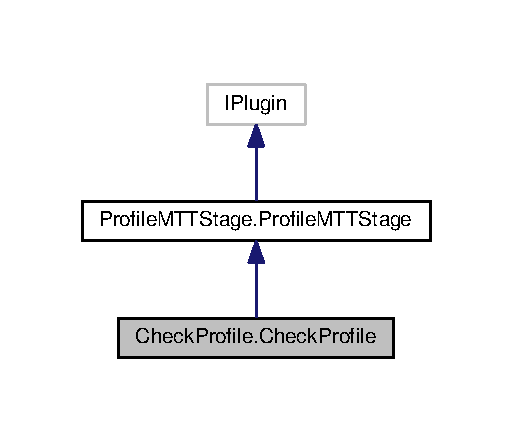
\includegraphics[width=246pt]{classCheckProfile_1_1CheckProfile__inherit__graph}
\end{center}
\end{figure}


Collaboration diagram for Check\-Profile.\-Check\-Profile\-:
\nopagebreak
\begin{figure}[H]
\begin{center}
\leavevmode
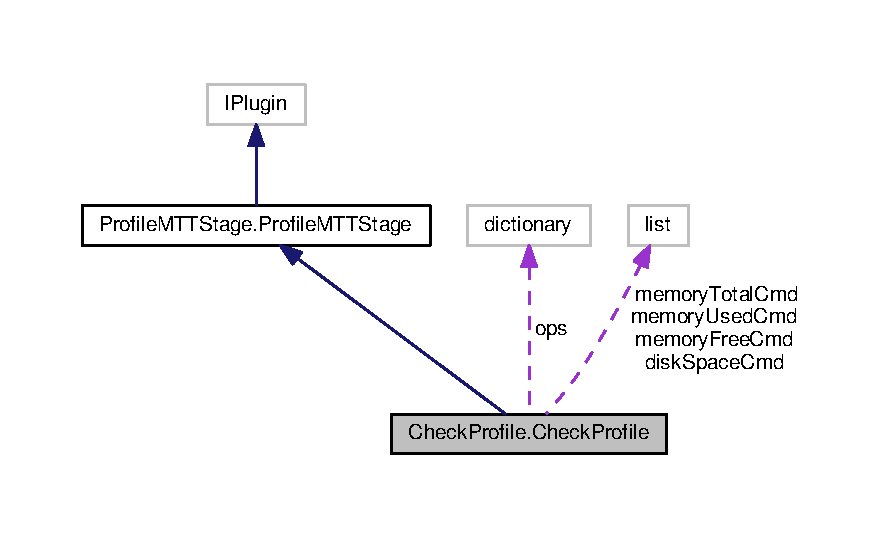
\includegraphics[width=350pt]{classCheckProfile_1_1CheckProfile__coll__graph}
\end{center}
\end{figure}
\subsection*{Public Member Functions}
\begin{DoxyCompactItemize}
\item 
def \hyperlink{classCheckProfile_1_1CheckProfile_a59610ed60307ee5ae57651f34bf9529f}{\-\_\-\-\_\-init\-\_\-\-\_\-}
\item 
def \hyperlink{classCheckProfile_1_1CheckProfile_a24038337f9ee0ed6741e38121fefc8c8}{activate}
\item 
def \hyperlink{classCheckProfile_1_1CheckProfile_ae499aa8259bdb20f403cb1bf84909939}{deactivate}
\item 
def \hyperlink{classCheckProfile_1_1CheckProfile_a7b456afd6026cac14021c21c5ad850f3}{print\-\_\-name}
\item 
def \hyperlink{classCheckProfile_1_1CheckProfile_aee55aa9f7021cb65097a5a485985df7c}{print\-\_\-options}
\item 
def \hyperlink{classCheckProfile_1_1CheckProfile_ad3ef683b23f6127a7a31373d00a7f1dc}{execute}
\end{DoxyCompactItemize}
\subsection*{Public Attributes}
\begin{DoxyCompactItemize}
\item 
\hyperlink{classCheckProfile_1_1CheckProfile_a60bdbb946d15fb43c2e465bb8a3fff99}{options}
\end{DoxyCompactItemize}
\subsection*{Static Public Attributes}
\begin{DoxyCompactItemize}
\item 
list \hyperlink{classCheckProfile_1_1CheckProfile_a074cbe798e2d4fa35fc83aa33a307b6c}{disk\-Space\-Cmd} = \mbox{[}\char`\"{}sh\char`\"{}, \char`\"{}-\/c\char`\"{}, \char`\"{}df -\/B\-M -\/-\/output=pcent D\-I\-S\-K $\vert$ grep -\/v Use\char`\"{}\mbox{]}
\item 
list \hyperlink{classCheckProfile_1_1CheckProfile_a8a9c2299135872cfccf2b0cb25ba854b}{memory\-Free\-Cmd} = \mbox{[}\char`\"{}sh\char`\"{}, \char`\"{}-\/c\char`\"{}, \char`\"{}free -\/h -\/o $\vert$ grep Mem\-: $\vert$ awk '\{print \$4\}'\char`\"{}\mbox{]}
\item 
list \hyperlink{classCheckProfile_1_1CheckProfile_a097bc2442305e7d6eebaff44a53c16f3}{memory\-Total\-Cmd} = \mbox{[}\char`\"{}sh\char`\"{}, \char`\"{}-\/c\char`\"{}, \char`\"{}free -\/h -\/o $\vert$ grep Mem\-: $\vert$ awk '\{print \$2\}'\char`\"{}\mbox{]}
\item 
list \hyperlink{classCheckProfile_1_1CheckProfile_a3c36cf35599b47c7158008533cc9cb39}{memory\-Used\-Cmd} = \mbox{[}\char`\"{}sh\char`\"{}, \char`\"{}-\/c\char`\"{}, \char`\"{}free -\/h -\/o $\vert$ grep Mem\-: $\vert$ awk '\{print \$3\}'\char`\"{}\mbox{]}
\item 
dictionary \hyperlink{classCheckProfile_1_1CheckProfile_aa4e92c1c6def969cc4a347111d4ef0de}{ops}
\end{DoxyCompactItemize}


\subsection{Detailed Description}


Definition at line 25 of file Check\-Profile.\-py.



\subsection{Constructor \& Destructor Documentation}
\hypertarget{classCheckProfile_1_1CheckProfile_a59610ed60307ee5ae57651f34bf9529f}{\index{Check\-Profile\-::\-Check\-Profile@{Check\-Profile\-::\-Check\-Profile}!\-\_\-\-\_\-init\-\_\-\-\_\-@{\-\_\-\-\_\-init\-\_\-\-\_\-}}
\index{\-\_\-\-\_\-init\-\_\-\-\_\-@{\-\_\-\-\_\-init\-\_\-\-\_\-}!CheckProfile::CheckProfile@{Check\-Profile\-::\-Check\-Profile}}
\subsubsection[{\-\_\-\-\_\-init\-\_\-\-\_\-}]{\setlength{\rightskip}{0pt plus 5cm}def Check\-Profile.\-Check\-Profile.\-\_\-\-\_\-init\-\_\-\-\_\- (
\begin{DoxyParamCaption}
\item[{}]{self}
\end{DoxyParamCaption}
)}}\label{classCheckProfile_1_1CheckProfile_a59610ed60307ee5ae57651f34bf9529f}


Definition at line 39 of file Check\-Profile.\-py.



\subsection{Member Function Documentation}
\hypertarget{classCheckProfile_1_1CheckProfile_a24038337f9ee0ed6741e38121fefc8c8}{\index{Check\-Profile\-::\-Check\-Profile@{Check\-Profile\-::\-Check\-Profile}!activate@{activate}}
\index{activate@{activate}!CheckProfile::CheckProfile@{Check\-Profile\-::\-Check\-Profile}}
\subsubsection[{activate}]{\setlength{\rightskip}{0pt plus 5cm}def Check\-Profile.\-Check\-Profile.\-activate (
\begin{DoxyParamCaption}
\item[{}]{self}
\end{DoxyParamCaption}
)}}\label{classCheckProfile_1_1CheckProfile_a24038337f9ee0ed6741e38121fefc8c8}


Definition at line 50 of file Check\-Profile.\-py.

\hypertarget{classCheckProfile_1_1CheckProfile_ae499aa8259bdb20f403cb1bf84909939}{\index{Check\-Profile\-::\-Check\-Profile@{Check\-Profile\-::\-Check\-Profile}!deactivate@{deactivate}}
\index{deactivate@{deactivate}!CheckProfile::CheckProfile@{Check\-Profile\-::\-Check\-Profile}}
\subsubsection[{deactivate}]{\setlength{\rightskip}{0pt plus 5cm}def Check\-Profile.\-Check\-Profile.\-deactivate (
\begin{DoxyParamCaption}
\item[{}]{self}
\end{DoxyParamCaption}
)}}\label{classCheckProfile_1_1CheckProfile_ae499aa8259bdb20f403cb1bf84909939}


Definition at line 56 of file Check\-Profile.\-py.

\hypertarget{classCheckProfile_1_1CheckProfile_ad3ef683b23f6127a7a31373d00a7f1dc}{\index{Check\-Profile\-::\-Check\-Profile@{Check\-Profile\-::\-Check\-Profile}!execute@{execute}}
\index{execute@{execute}!CheckProfile::CheckProfile@{Check\-Profile\-::\-Check\-Profile}}
\subsubsection[{execute}]{\setlength{\rightskip}{0pt plus 5cm}def Check\-Profile.\-Check\-Profile.\-execute (
\begin{DoxyParamCaption}
\item[{}]{self, }
\item[{}]{log, }
\item[{}]{keyvals, }
\item[{}]{test\-Def}
\end{DoxyParamCaption}
)}}\label{classCheckProfile_1_1CheckProfile_ad3ef683b23f6127a7a31373d00a7f1dc}


Definition at line 69 of file Check\-Profile.\-py.

\hypertarget{classCheckProfile_1_1CheckProfile_a7b456afd6026cac14021c21c5ad850f3}{\index{Check\-Profile\-::\-Check\-Profile@{Check\-Profile\-::\-Check\-Profile}!print\-\_\-name@{print\-\_\-name}}
\index{print\-\_\-name@{print\-\_\-name}!CheckProfile::CheckProfile@{Check\-Profile\-::\-Check\-Profile}}
\subsubsection[{print\-\_\-name}]{\setlength{\rightskip}{0pt plus 5cm}def Check\-Profile.\-Check\-Profile.\-print\-\_\-name (
\begin{DoxyParamCaption}
\item[{}]{self}
\end{DoxyParamCaption}
)}}\label{classCheckProfile_1_1CheckProfile_a7b456afd6026cac14021c21c5ad850f3}


Definition at line 60 of file Check\-Profile.\-py.

\hypertarget{classCheckProfile_1_1CheckProfile_aee55aa9f7021cb65097a5a485985df7c}{\index{Check\-Profile\-::\-Check\-Profile@{Check\-Profile\-::\-Check\-Profile}!print\-\_\-options@{print\-\_\-options}}
\index{print\-\_\-options@{print\-\_\-options}!CheckProfile::CheckProfile@{Check\-Profile\-::\-Check\-Profile}}
\subsubsection[{print\-\_\-options}]{\setlength{\rightskip}{0pt plus 5cm}def Check\-Profile.\-Check\-Profile.\-print\-\_\-options (
\begin{DoxyParamCaption}
\item[{}]{self, }
\item[{}]{test\-Def, }
\item[{}]{prefix}
\end{DoxyParamCaption}
)}}\label{classCheckProfile_1_1CheckProfile_aee55aa9f7021cb65097a5a485985df7c}


Definition at line 63 of file Check\-Profile.\-py.



\subsection{Member Data Documentation}
\hypertarget{classCheckProfile_1_1CheckProfile_a074cbe798e2d4fa35fc83aa33a307b6c}{\index{Check\-Profile\-::\-Check\-Profile@{Check\-Profile\-::\-Check\-Profile}!disk\-Space\-Cmd@{disk\-Space\-Cmd}}
\index{disk\-Space\-Cmd@{disk\-Space\-Cmd}!CheckProfile::CheckProfile@{Check\-Profile\-::\-Check\-Profile}}
\subsubsection[{disk\-Space\-Cmd}]{\setlength{\rightskip}{0pt plus 5cm}list Check\-Profile.\-Check\-Profile.\-disk\-Space\-Cmd = \mbox{[}\char`\"{}sh\char`\"{}, \char`\"{}-\/c\char`\"{}, \char`\"{}df -\/B\-M -\/-\/output=pcent D\-I\-S\-K $\vert$ grep -\/v Use\char`\"{}\mbox{]}\hspace{0.3cm}{\ttfamily [static]}}}\label{classCheckProfile_1_1CheckProfile_a074cbe798e2d4fa35fc83aa33a307b6c}


Definition at line 27 of file Check\-Profile.\-py.

\hypertarget{classCheckProfile_1_1CheckProfile_a8a9c2299135872cfccf2b0cb25ba854b}{\index{Check\-Profile\-::\-Check\-Profile@{Check\-Profile\-::\-Check\-Profile}!memory\-Free\-Cmd@{memory\-Free\-Cmd}}
\index{memory\-Free\-Cmd@{memory\-Free\-Cmd}!CheckProfile::CheckProfile@{Check\-Profile\-::\-Check\-Profile}}
\subsubsection[{memory\-Free\-Cmd}]{\setlength{\rightskip}{0pt plus 5cm}list Check\-Profile.\-Check\-Profile.\-memory\-Free\-Cmd = \mbox{[}\char`\"{}sh\char`\"{}, \char`\"{}-\/c\char`\"{}, \char`\"{}free -\/h -\/o $\vert$ grep Mem\-: $\vert$ awk '\{print \$4\}'\char`\"{}\mbox{]}\hspace{0.3cm}{\ttfamily [static]}}}\label{classCheckProfile_1_1CheckProfile_a8a9c2299135872cfccf2b0cb25ba854b}


Definition at line 28 of file Check\-Profile.\-py.

\hypertarget{classCheckProfile_1_1CheckProfile_a097bc2442305e7d6eebaff44a53c16f3}{\index{Check\-Profile\-::\-Check\-Profile@{Check\-Profile\-::\-Check\-Profile}!memory\-Total\-Cmd@{memory\-Total\-Cmd}}
\index{memory\-Total\-Cmd@{memory\-Total\-Cmd}!CheckProfile::CheckProfile@{Check\-Profile\-::\-Check\-Profile}}
\subsubsection[{memory\-Total\-Cmd}]{\setlength{\rightskip}{0pt plus 5cm}list Check\-Profile.\-Check\-Profile.\-memory\-Total\-Cmd = \mbox{[}\char`\"{}sh\char`\"{}, \char`\"{}-\/c\char`\"{}, \char`\"{}free -\/h -\/o $\vert$ grep Mem\-: $\vert$ awk '\{print \$2\}'\char`\"{}\mbox{]}\hspace{0.3cm}{\ttfamily [static]}}}\label{classCheckProfile_1_1CheckProfile_a097bc2442305e7d6eebaff44a53c16f3}


Definition at line 29 of file Check\-Profile.\-py.

\hypertarget{classCheckProfile_1_1CheckProfile_a3c36cf35599b47c7158008533cc9cb39}{\index{Check\-Profile\-::\-Check\-Profile@{Check\-Profile\-::\-Check\-Profile}!memory\-Used\-Cmd@{memory\-Used\-Cmd}}
\index{memory\-Used\-Cmd@{memory\-Used\-Cmd}!CheckProfile::CheckProfile@{Check\-Profile\-::\-Check\-Profile}}
\subsubsection[{memory\-Used\-Cmd}]{\setlength{\rightskip}{0pt plus 5cm}list Check\-Profile.\-Check\-Profile.\-memory\-Used\-Cmd = \mbox{[}\char`\"{}sh\char`\"{}, \char`\"{}-\/c\char`\"{}, \char`\"{}free -\/h -\/o $\vert$ grep Mem\-: $\vert$ awk '\{print \$3\}'\char`\"{}\mbox{]}\hspace{0.3cm}{\ttfamily [static]}}}\label{classCheckProfile_1_1CheckProfile_a3c36cf35599b47c7158008533cc9cb39}


Definition at line 30 of file Check\-Profile.\-py.

\hypertarget{classCheckProfile_1_1CheckProfile_aa4e92c1c6def969cc4a347111d4ef0de}{\index{Check\-Profile\-::\-Check\-Profile@{Check\-Profile\-::\-Check\-Profile}!ops@{ops}}
\index{ops@{ops}!CheckProfile::CheckProfile@{Check\-Profile\-::\-Check\-Profile}}
\subsubsection[{ops}]{\setlength{\rightskip}{0pt plus 5cm}dictionary Check\-Profile.\-Check\-Profile.\-ops\hspace{0.3cm}{\ttfamily [static]}}}\label{classCheckProfile_1_1CheckProfile_aa4e92c1c6def969cc4a347111d4ef0de}
{\bfseries Initial value\-:}
\begin{DoxyCode}
1 = \{ \textcolor{stringliteral}{'>'}: operator.gt,
2             \textcolor{stringliteral}{'<'}: operator.lt,
3             \textcolor{stringliteral}{'>='}: operator.ge,
4             \textcolor{stringliteral}{'<='}: operator.le,
5             \textcolor{stringliteral}{'='}: operator.eq
6     \}
\end{DoxyCode}


Definition at line 32 of file Check\-Profile.\-py.

\hypertarget{classCheckProfile_1_1CheckProfile_a60bdbb946d15fb43c2e465bb8a3fff99}{\index{Check\-Profile\-::\-Check\-Profile@{Check\-Profile\-::\-Check\-Profile}!options@{options}}
\index{options@{options}!CheckProfile::CheckProfile@{Check\-Profile\-::\-Check\-Profile}}
\subsubsection[{options}]{\setlength{\rightskip}{0pt plus 5cm}Check\-Profile.\-Check\-Profile.\-options}}\label{classCheckProfile_1_1CheckProfile_a60bdbb946d15fb43c2e465bb8a3fff99}


Definition at line 42 of file Check\-Profile.\-py.



The documentation for this class was generated from the following file\-:\begin{DoxyCompactItemize}
\item 
/home/travis/build/open-\/mpi/mtt/pylib/\-Stages/\-Profile/\hyperlink{CheckProfile_8py}{Check\-Profile.\-py}\end{DoxyCompactItemize}

\hypertarget{classCNCMTTTool_1_1CNCMTTTool}{\section{C\-N\-C\-M\-T\-T\-Tool.\-C\-N\-C\-M\-T\-T\-Tool Class Reference}
\label{classCNCMTTTool_1_1CNCMTTTool}\index{C\-N\-C\-M\-T\-T\-Tool.\-C\-N\-C\-M\-T\-T\-Tool@{C\-N\-C\-M\-T\-T\-Tool.\-C\-N\-C\-M\-T\-T\-Tool}}
}


Inheritance diagram for C\-N\-C\-M\-T\-T\-Tool.\-C\-N\-C\-M\-T\-T\-Tool\-:
\nopagebreak
\begin{figure}[H]
\begin{center}
\leavevmode
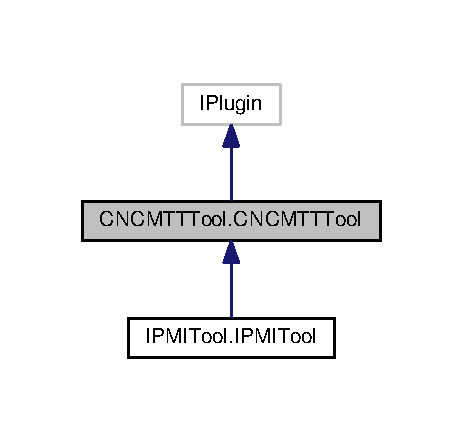
\includegraphics[width=222pt]{classCNCMTTTool_1_1CNCMTTTool__inherit__graph}
\end{center}
\end{figure}


Collaboration diagram for C\-N\-C\-M\-T\-T\-Tool.\-C\-N\-C\-M\-T\-T\-Tool\-:
\nopagebreak
\begin{figure}[H]
\begin{center}
\leavevmode
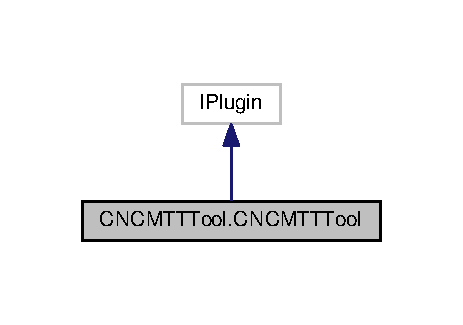
\includegraphics[width=222pt]{classCNCMTTTool_1_1CNCMTTTool__coll__graph}
\end{center}
\end{figure}
\subsection*{Public Member Functions}
\begin{DoxyCompactItemize}
\item 
def \hyperlink{classCNCMTTTool_1_1CNCMTTTool_a9f2d86b7cd592cae84be27e90d65f862}{\-\_\-\-\_\-init\-\_\-\-\_\-}
\item 
def \hyperlink{classCNCMTTTool_1_1CNCMTTTool_a664d4cdf650553342d45bf04981a8e2d}{print\-\_\-name}
\end{DoxyCompactItemize}


\subsection{Detailed Description}


Definition at line 19 of file C\-N\-C\-M\-T\-T\-Tool.\-py.



\subsection{Constructor \& Destructor Documentation}
\hypertarget{classCNCMTTTool_1_1CNCMTTTool_a9f2d86b7cd592cae84be27e90d65f862}{\index{C\-N\-C\-M\-T\-T\-Tool\-::\-C\-N\-C\-M\-T\-T\-Tool@{C\-N\-C\-M\-T\-T\-Tool\-::\-C\-N\-C\-M\-T\-T\-Tool}!\-\_\-\-\_\-init\-\_\-\-\_\-@{\-\_\-\-\_\-init\-\_\-\-\_\-}}
\index{\-\_\-\-\_\-init\-\_\-\-\_\-@{\-\_\-\-\_\-init\-\_\-\-\_\-}!CNCMTTTool::CNCMTTTool@{C\-N\-C\-M\-T\-T\-Tool\-::\-C\-N\-C\-M\-T\-T\-Tool}}
\subsubsection[{\-\_\-\-\_\-init\-\_\-\-\_\-}]{\setlength{\rightskip}{0pt plus 5cm}def C\-N\-C\-M\-T\-T\-Tool.\-C\-N\-C\-M\-T\-T\-Tool.\-\_\-\-\_\-init\-\_\-\-\_\- (
\begin{DoxyParamCaption}
\item[{}]{self}
\end{DoxyParamCaption}
)}}\label{classCNCMTTTool_1_1CNCMTTTool_a9f2d86b7cd592cae84be27e90d65f862}


Definition at line 20 of file C\-N\-C\-M\-T\-T\-Tool.\-py.



\subsection{Member Function Documentation}
\hypertarget{classCNCMTTTool_1_1CNCMTTTool_a664d4cdf650553342d45bf04981a8e2d}{\index{C\-N\-C\-M\-T\-T\-Tool\-::\-C\-N\-C\-M\-T\-T\-Tool@{C\-N\-C\-M\-T\-T\-Tool\-::\-C\-N\-C\-M\-T\-T\-Tool}!print\-\_\-name@{print\-\_\-name}}
\index{print\-\_\-name@{print\-\_\-name}!CNCMTTTool::CNCMTTTool@{C\-N\-C\-M\-T\-T\-Tool\-::\-C\-N\-C\-M\-T\-T\-Tool}}
\subsubsection[{print\-\_\-name}]{\setlength{\rightskip}{0pt plus 5cm}def C\-N\-C\-M\-T\-T\-Tool.\-C\-N\-C\-M\-T\-T\-Tool.\-print\-\_\-name (
\begin{DoxyParamCaption}
\item[{}]{self}
\end{DoxyParamCaption}
)}}\label{classCNCMTTTool_1_1CNCMTTTool_a664d4cdf650553342d45bf04981a8e2d}


Definition at line 24 of file C\-N\-C\-M\-T\-T\-Tool.\-py.



The documentation for this class was generated from the following file\-:\begin{DoxyCompactItemize}
\item 
/home/travis/build/open-\/mpi/mtt/pylib/\-Tools/\-C\-N\-C/\hyperlink{CNCMTTTool_8py}{C\-N\-C\-M\-T\-T\-Tool.\-py}\end{DoxyCompactItemize}

\hypertarget{classcombinatorial_1_1CombinatorialEx}{\section{combinatorial.\-Combinatorial\-Ex Class Reference}
\label{classcombinatorial_1_1CombinatorialEx}\index{combinatorial.\-Combinatorial\-Ex@{combinatorial.\-Combinatorial\-Ex}}
}


Inheritance diagram for combinatorial.\-Combinatorial\-Ex\-:
\nopagebreak
\begin{figure}[H]
\begin{center}
\leavevmode
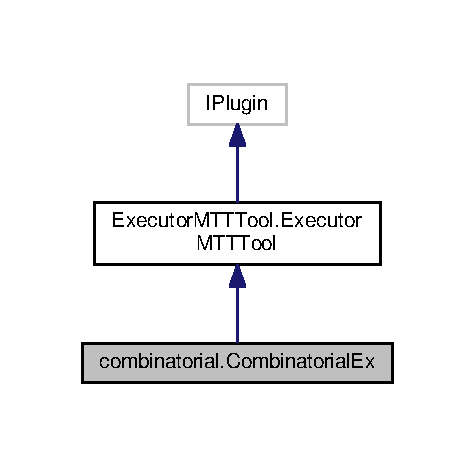
\includegraphics[width=228pt]{classcombinatorial_1_1CombinatorialEx__inherit__graph}
\end{center}
\end{figure}


Collaboration diagram for combinatorial.\-Combinatorial\-Ex\-:
\nopagebreak
\begin{figure}[H]
\begin{center}
\leavevmode
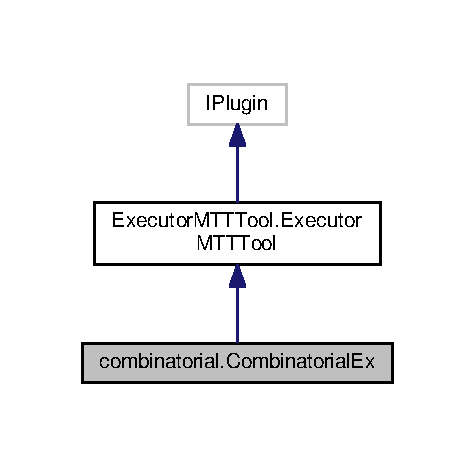
\includegraphics[width=228pt]{classcombinatorial_1_1CombinatorialEx__coll__graph}
\end{center}
\end{figure}
\subsection*{Public Member Functions}
\begin{DoxyCompactItemize}
\item 
def \hyperlink{classcombinatorial_1_1CombinatorialEx_a9a4fbfcf64b1204c14509d348dd23b5d}{\-\_\-\-\_\-init\-\_\-\-\_\-}
\item 
def \hyperlink{classcombinatorial_1_1CombinatorialEx_a8d0b7c0da355183d8124871bee76b0bd}{activate}
\item 
def \hyperlink{classcombinatorial_1_1CombinatorialEx_ad53efcff93773cce7ed9cfc2fef38ab3}{deactivate}
\item 
def \hyperlink{classcombinatorial_1_1CombinatorialEx_a19f6321bf42ab92280c5e3b0a3af89d0}{print\-\_\-name}
\item 
def \hyperlink{classcombinatorial_1_1CombinatorialEx_ae802ad33a050ada42292e7c80fb3e486}{print\-\_\-options}
\item 
def \hyperlink{classcombinatorial_1_1CombinatorialEx_ac0216f0d0041c35a91e01ac9dafd49da}{create\-Ini\-Log}
\item 
def \hyperlink{classcombinatorial_1_1CombinatorialEx_a5a5fbd1692c100374ee458e4babc9832}{execute}
\end{DoxyCompactItemize}
\subsection*{Public Attributes}
\begin{DoxyCompactItemize}
\item 
\hyperlink{classcombinatorial_1_1CombinatorialEx_a20eda525b3947495bb6084c560dcca27}{options}
\item 
\hyperlink{classcombinatorial_1_1CombinatorialEx_ab5c27fece8991a34f47e85870637fc91}{parser}
\item 
\hyperlink{classcombinatorial_1_1CombinatorialEx_a24b3bc621a8380e406bade192bc371d4}{temp\-Dir}
\item 
\hyperlink{classcombinatorial_1_1CombinatorialEx_a68e6ac6cba4ab4161dd854323e549afd}{base\-Ini\-File}
\item 
\hyperlink{classcombinatorial_1_1CombinatorialEx_a3de3f7da4c201525da8452258df0bc7b}{run\-Log}
\item 
\hyperlink{classcombinatorial_1_1CombinatorialEx_a961a46d05fda7be52ea74a5f69df57e2}{ini\-Log}
\end{DoxyCompactItemize}


\subsection{Detailed Description}


Definition at line 33 of file combinatorial.\-py.



\subsection{Constructor \& Destructor Documentation}
\hypertarget{classcombinatorial_1_1CombinatorialEx_a9a4fbfcf64b1204c14509d348dd23b5d}{\index{combinatorial\-::\-Combinatorial\-Ex@{combinatorial\-::\-Combinatorial\-Ex}!\-\_\-\-\_\-init\-\_\-\-\_\-@{\-\_\-\-\_\-init\-\_\-\-\_\-}}
\index{\-\_\-\-\_\-init\-\_\-\-\_\-@{\-\_\-\-\_\-init\-\_\-\-\_\-}!combinatorial::CombinatorialEx@{combinatorial\-::\-Combinatorial\-Ex}}
\subsubsection[{\-\_\-\-\_\-init\-\_\-\-\_\-}]{\setlength{\rightskip}{0pt plus 5cm}def combinatorial.\-Combinatorial\-Ex.\-\_\-\-\_\-init\-\_\-\-\_\- (
\begin{DoxyParamCaption}
\item[{}]{self}
\end{DoxyParamCaption}
)}}\label{classcombinatorial_1_1CombinatorialEx_a9a4fbfcf64b1204c14509d348dd23b5d}


Definition at line 35 of file combinatorial.\-py.



\subsection{Member Function Documentation}
\hypertarget{classcombinatorial_1_1CombinatorialEx_a8d0b7c0da355183d8124871bee76b0bd}{\index{combinatorial\-::\-Combinatorial\-Ex@{combinatorial\-::\-Combinatorial\-Ex}!activate@{activate}}
\index{activate@{activate}!combinatorial::CombinatorialEx@{combinatorial\-::\-Combinatorial\-Ex}}
\subsubsection[{activate}]{\setlength{\rightskip}{0pt plus 5cm}def combinatorial.\-Combinatorial\-Ex.\-activate (
\begin{DoxyParamCaption}
\item[{}]{self}
\end{DoxyParamCaption}
)}}\label{classcombinatorial_1_1CombinatorialEx_a8d0b7c0da355183d8124871bee76b0bd}


Definition at line 47 of file combinatorial.\-py.

\hypertarget{classcombinatorial_1_1CombinatorialEx_ac0216f0d0041c35a91e01ac9dafd49da}{\index{combinatorial\-::\-Combinatorial\-Ex@{combinatorial\-::\-Combinatorial\-Ex}!create\-Ini\-Log@{create\-Ini\-Log}}
\index{create\-Ini\-Log@{create\-Ini\-Log}!combinatorial::CombinatorialEx@{combinatorial\-::\-Combinatorial\-Ex}}
\subsubsection[{create\-Ini\-Log}]{\setlength{\rightskip}{0pt plus 5cm}def combinatorial.\-Combinatorial\-Ex.\-create\-Ini\-Log (
\begin{DoxyParamCaption}
\item[{}]{self, }
\item[{}]{test\-Def}
\end{DoxyParamCaption}
)}}\label{classcombinatorial_1_1CombinatorialEx_ac0216f0d0041c35a91e01ac9dafd49da}


Definition at line 68 of file combinatorial.\-py.



Here is the caller graph for this function\-:
\nopagebreak
\begin{figure}[H]
\begin{center}
\leavevmode
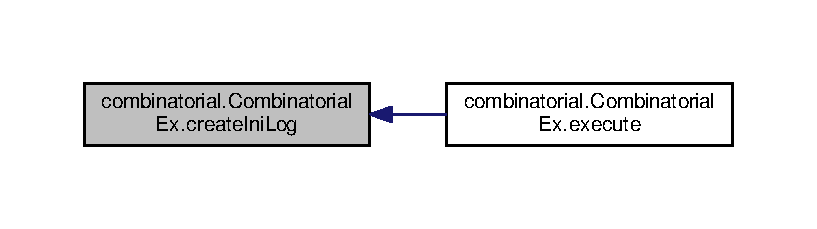
\includegraphics[width=350pt]{classcombinatorial_1_1CombinatorialEx_ac0216f0d0041c35a91e01ac9dafd49da_icgraph}
\end{center}
\end{figure}


\hypertarget{classcombinatorial_1_1CombinatorialEx_ad53efcff93773cce7ed9cfc2fef38ab3}{\index{combinatorial\-::\-Combinatorial\-Ex@{combinatorial\-::\-Combinatorial\-Ex}!deactivate@{deactivate}}
\index{deactivate@{deactivate}!combinatorial::CombinatorialEx@{combinatorial\-::\-Combinatorial\-Ex}}
\subsubsection[{deactivate}]{\setlength{\rightskip}{0pt plus 5cm}def combinatorial.\-Combinatorial\-Ex.\-deactivate (
\begin{DoxyParamCaption}
\item[{}]{self}
\end{DoxyParamCaption}
)}}\label{classcombinatorial_1_1CombinatorialEx_ad53efcff93773cce7ed9cfc2fef38ab3}


Definition at line 52 of file combinatorial.\-py.

\hypertarget{classcombinatorial_1_1CombinatorialEx_a5a5fbd1692c100374ee458e4babc9832}{\index{combinatorial\-::\-Combinatorial\-Ex@{combinatorial\-::\-Combinatorial\-Ex}!execute@{execute}}
\index{execute@{execute}!combinatorial::CombinatorialEx@{combinatorial\-::\-Combinatorial\-Ex}}
\subsubsection[{execute}]{\setlength{\rightskip}{0pt plus 5cm}def combinatorial.\-Combinatorial\-Ex.\-execute (
\begin{DoxyParamCaption}
\item[{}]{self, }
\item[{}]{test\-Def}
\end{DoxyParamCaption}
)}}\label{classcombinatorial_1_1CombinatorialEx_a5a5fbd1692c100374ee458e4babc9832}


Definition at line 171 of file combinatorial.\-py.



Here is the call graph for this function\-:
\nopagebreak
\begin{figure}[H]
\begin{center}
\leavevmode
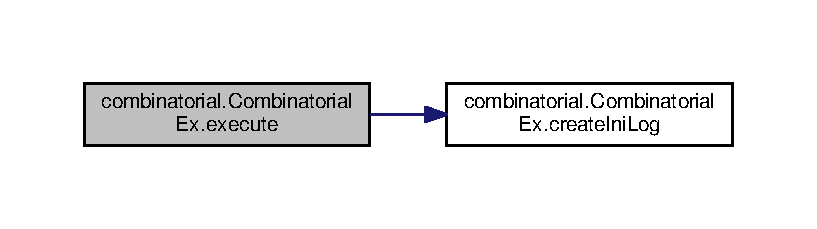
\includegraphics[width=350pt]{classcombinatorial_1_1CombinatorialEx_a5a5fbd1692c100374ee458e4babc9832_cgraph}
\end{center}
\end{figure}


\hypertarget{classcombinatorial_1_1CombinatorialEx_a19f6321bf42ab92280c5e3b0a3af89d0}{\index{combinatorial\-::\-Combinatorial\-Ex@{combinatorial\-::\-Combinatorial\-Ex}!print\-\_\-name@{print\-\_\-name}}
\index{print\-\_\-name@{print\-\_\-name}!combinatorial::CombinatorialEx@{combinatorial\-::\-Combinatorial\-Ex}}
\subsubsection[{print\-\_\-name}]{\setlength{\rightskip}{0pt plus 5cm}def combinatorial.\-Combinatorial\-Ex.\-print\-\_\-name (
\begin{DoxyParamCaption}
\item[{}]{self}
\end{DoxyParamCaption}
)}}\label{classcombinatorial_1_1CombinatorialEx_a19f6321bf42ab92280c5e3b0a3af89d0}


Definition at line 56 of file combinatorial.\-py.

\hypertarget{classcombinatorial_1_1CombinatorialEx_ae802ad33a050ada42292e7c80fb3e486}{\index{combinatorial\-::\-Combinatorial\-Ex@{combinatorial\-::\-Combinatorial\-Ex}!print\-\_\-options@{print\-\_\-options}}
\index{print\-\_\-options@{print\-\_\-options}!combinatorial::CombinatorialEx@{combinatorial\-::\-Combinatorial\-Ex}}
\subsubsection[{print\-\_\-options}]{\setlength{\rightskip}{0pt plus 5cm}def combinatorial.\-Combinatorial\-Ex.\-print\-\_\-options (
\begin{DoxyParamCaption}
\item[{}]{self, }
\item[{}]{test\-Def, }
\item[{}]{prefix}
\end{DoxyParamCaption}
)}}\label{classcombinatorial_1_1CombinatorialEx_ae802ad33a050ada42292e7c80fb3e486}


Definition at line 59 of file combinatorial.\-py.



\subsection{Member Data Documentation}
\hypertarget{classcombinatorial_1_1CombinatorialEx_a68e6ac6cba4ab4161dd854323e549afd}{\index{combinatorial\-::\-Combinatorial\-Ex@{combinatorial\-::\-Combinatorial\-Ex}!base\-Ini\-File@{base\-Ini\-File}}
\index{base\-Ini\-File@{base\-Ini\-File}!combinatorial::CombinatorialEx@{combinatorial\-::\-Combinatorial\-Ex}}
\subsubsection[{base\-Ini\-File}]{\setlength{\rightskip}{0pt plus 5cm}combinatorial.\-Combinatorial\-Ex.\-base\-Ini\-File}}\label{classcombinatorial_1_1CombinatorialEx_a68e6ac6cba4ab4161dd854323e549afd}


Definition at line 43 of file combinatorial.\-py.

\hypertarget{classcombinatorial_1_1CombinatorialEx_a961a46d05fda7be52ea74a5f69df57e2}{\index{combinatorial\-::\-Combinatorial\-Ex@{combinatorial\-::\-Combinatorial\-Ex}!ini\-Log@{ini\-Log}}
\index{ini\-Log@{ini\-Log}!combinatorial::CombinatorialEx@{combinatorial\-::\-Combinatorial\-Ex}}
\subsubsection[{ini\-Log}]{\setlength{\rightskip}{0pt plus 5cm}combinatorial.\-Combinatorial\-Ex.\-ini\-Log}}\label{classcombinatorial_1_1CombinatorialEx_a961a46d05fda7be52ea74a5f69df57e2}


Definition at line 45 of file combinatorial.\-py.

\hypertarget{classcombinatorial_1_1CombinatorialEx_a20eda525b3947495bb6084c560dcca27}{\index{combinatorial\-::\-Combinatorial\-Ex@{combinatorial\-::\-Combinatorial\-Ex}!options@{options}}
\index{options@{options}!combinatorial::CombinatorialEx@{combinatorial\-::\-Combinatorial\-Ex}}
\subsubsection[{options}]{\setlength{\rightskip}{0pt plus 5cm}combinatorial.\-Combinatorial\-Ex.\-options}}\label{classcombinatorial_1_1CombinatorialEx_a20eda525b3947495bb6084c560dcca27}


Definition at line 38 of file combinatorial.\-py.

\hypertarget{classcombinatorial_1_1CombinatorialEx_ab5c27fece8991a34f47e85870637fc91}{\index{combinatorial\-::\-Combinatorial\-Ex@{combinatorial\-::\-Combinatorial\-Ex}!parser@{parser}}
\index{parser@{parser}!combinatorial::CombinatorialEx@{combinatorial\-::\-Combinatorial\-Ex}}
\subsubsection[{parser}]{\setlength{\rightskip}{0pt plus 5cm}combinatorial.\-Combinatorial\-Ex.\-parser}}\label{classcombinatorial_1_1CombinatorialEx_ab5c27fece8991a34f47e85870637fc91}


Definition at line 39 of file combinatorial.\-py.

\hypertarget{classcombinatorial_1_1CombinatorialEx_a3de3f7da4c201525da8452258df0bc7b}{\index{combinatorial\-::\-Combinatorial\-Ex@{combinatorial\-::\-Combinatorial\-Ex}!run\-Log@{run\-Log}}
\index{run\-Log@{run\-Log}!combinatorial::CombinatorialEx@{combinatorial\-::\-Combinatorial\-Ex}}
\subsubsection[{run\-Log}]{\setlength{\rightskip}{0pt plus 5cm}combinatorial.\-Combinatorial\-Ex.\-run\-Log}}\label{classcombinatorial_1_1CombinatorialEx_a3de3f7da4c201525da8452258df0bc7b}


Definition at line 44 of file combinatorial.\-py.

\hypertarget{classcombinatorial_1_1CombinatorialEx_a24b3bc621a8380e406bade192bc371d4}{\index{combinatorial\-::\-Combinatorial\-Ex@{combinatorial\-::\-Combinatorial\-Ex}!temp\-Dir@{temp\-Dir}}
\index{temp\-Dir@{temp\-Dir}!combinatorial::CombinatorialEx@{combinatorial\-::\-Combinatorial\-Ex}}
\subsubsection[{temp\-Dir}]{\setlength{\rightskip}{0pt plus 5cm}combinatorial.\-Combinatorial\-Ex.\-temp\-Dir}}\label{classcombinatorial_1_1CombinatorialEx_a24b3bc621a8380e406bade192bc371d4}


Definition at line 42 of file combinatorial.\-py.



The documentation for this class was generated from the following file\-:\begin{DoxyCompactItemize}
\item 
/home/travis/build/open-\/mpi/mtt/pylib/\-Tools/\-Executor/\hyperlink{combinatorial_8py}{combinatorial.\-py}\end{DoxyCompactItemize}

\hypertarget{classCompilers_1_1Compilers}{\section{Compilers.\-Compilers Class Reference}
\label{classCompilers_1_1Compilers}\index{Compilers.\-Compilers@{Compilers.\-Compilers}}
}


Inheritance diagram for Compilers.\-Compilers\-:
\nopagebreak
\begin{figure}[H]
\begin{center}
\leavevmode
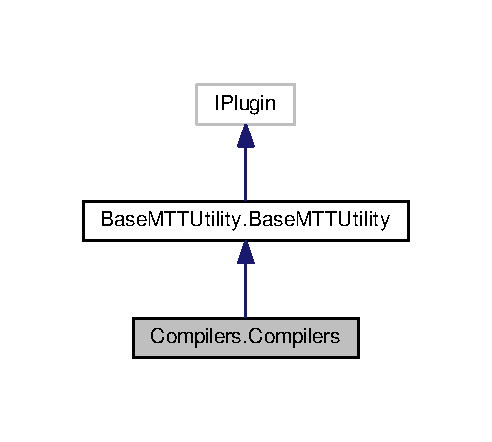
\includegraphics[width=236pt]{classCompilers_1_1Compilers__inherit__graph}
\end{center}
\end{figure}


Collaboration diagram for Compilers.\-Compilers\-:
\nopagebreak
\begin{figure}[H]
\begin{center}
\leavevmode
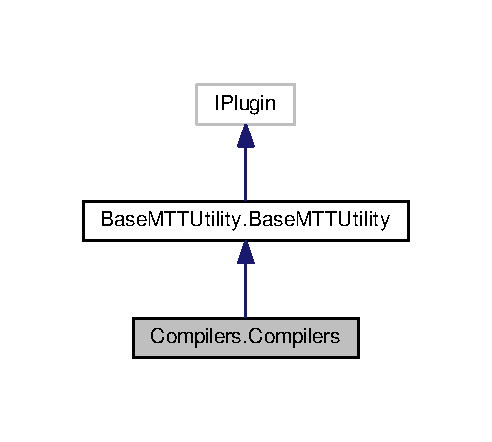
\includegraphics[width=236pt]{classCompilers_1_1Compilers__coll__graph}
\end{center}
\end{figure}
\subsection*{Public Member Functions}
\begin{DoxyCompactItemize}
\item 
def \hyperlink{classCompilers_1_1Compilers_a401d7750736badfcabbcdd39909109c7}{\-\_\-\-\_\-init\-\_\-\-\_\-}
\item 
def \hyperlink{classCompilers_1_1Compilers_aabd91a4eeb39804bbddba7c5bb1b6ec0}{print\-\_\-name}
\item 
def \hyperlink{classCompilers_1_1Compilers_a152a2bd6caf05098ebdfd2e336c1f71b}{print\-\_\-options}
\item 
def \hyperlink{classCompilers_1_1Compilers_a85044d54e6b66cb5f29328a75f5bf446}{execute}
\item 
def \hyperlink{classCompilers_1_1Compilers_aac1f107915d98d9b076c68a7ebc2ec48}{check\-\_\-compile}
\item 
def \hyperlink{classCompilers_1_1Compilers_a82b789e14047fa9d8027c9df59c95dca}{check\-\_\-c\-\_\-ifdef}
\item 
def \hyperlink{classCompilers_1_1Compilers_a5a8137663ccef6cb4a82c2636d93ce3b}{check\-\_\-c\-\_\-if}
\item 
def \hyperlink{classCompilers_1_1Compilers_a3a65f6da74cda8747cfc7af58ad2e1ee}{check\-\_\-version}
\end{DoxyCompactItemize}
\subsection*{Public Attributes}
\begin{DoxyCompactItemize}
\item 
\hyperlink{classCompilers_1_1Compilers_a29d4fb86feaa70cccd5d6b8852421767}{options}
\end{DoxyCompactItemize}


\subsection{Detailed Description}


Definition at line 19 of file Compilers.\-py.



\subsection{Constructor \& Destructor Documentation}
\hypertarget{classCompilers_1_1Compilers_a401d7750736badfcabbcdd39909109c7}{\index{Compilers\-::\-Compilers@{Compilers\-::\-Compilers}!\-\_\-\-\_\-init\-\_\-\-\_\-@{\-\_\-\-\_\-init\-\_\-\-\_\-}}
\index{\-\_\-\-\_\-init\-\_\-\-\_\-@{\-\_\-\-\_\-init\-\_\-\-\_\-}!Compilers::Compilers@{Compilers\-::\-Compilers}}
\subsubsection[{\-\_\-\-\_\-init\-\_\-\-\_\-}]{\setlength{\rightskip}{0pt plus 5cm}def Compilers.\-Compilers.\-\_\-\-\_\-init\-\_\-\-\_\- (
\begin{DoxyParamCaption}
\item[{}]{self}
\end{DoxyParamCaption}
)}}\label{classCompilers_1_1Compilers_a401d7750736badfcabbcdd39909109c7}


Definition at line 20 of file Compilers.\-py.



\subsection{Member Function Documentation}
\hypertarget{classCompilers_1_1Compilers_a5a8137663ccef6cb4a82c2636d93ce3b}{\index{Compilers\-::\-Compilers@{Compilers\-::\-Compilers}!check\-\_\-c\-\_\-if@{check\-\_\-c\-\_\-if}}
\index{check\-\_\-c\-\_\-if@{check\-\_\-c\-\_\-if}!Compilers::Compilers@{Compilers\-::\-Compilers}}
\subsubsection[{check\-\_\-c\-\_\-if}]{\setlength{\rightskip}{0pt plus 5cm}def Compilers.\-Compilers.\-check\-\_\-c\-\_\-if (
\begin{DoxyParamCaption}
\item[{}]{self, }
\item[{}]{test\-Def, }
\item[{}]{macro, }
\item[{}]{compiler}
\end{DoxyParamCaption}
)}}\label{classCompilers_1_1Compilers_a5a8137663ccef6cb4a82c2636d93ce3b}


Definition at line 204 of file Compilers.\-py.



Here is the call graph for this function\-:
\nopagebreak
\begin{figure}[H]
\begin{center}
\leavevmode
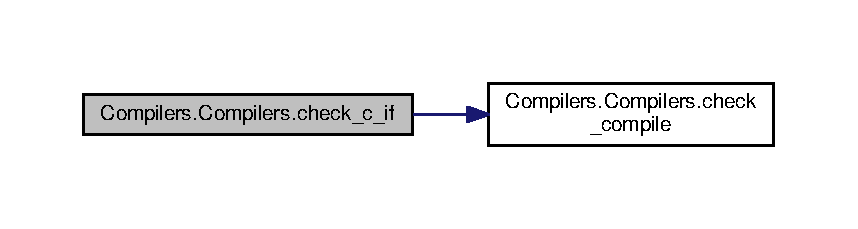
\includegraphics[width=350pt]{classCompilers_1_1Compilers_a5a8137663ccef6cb4a82c2636d93ce3b_cgraph}
\end{center}
\end{figure}




Here is the caller graph for this function\-:
\nopagebreak
\begin{figure}[H]
\begin{center}
\leavevmode
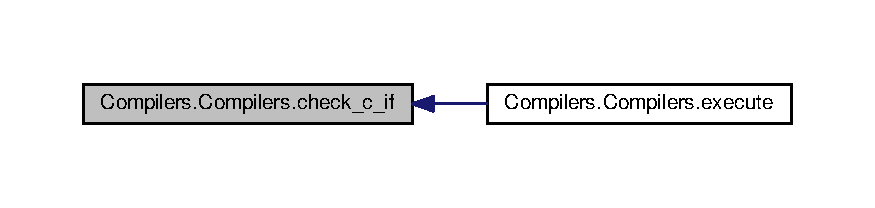
\includegraphics[width=350pt]{classCompilers_1_1Compilers_a5a8137663ccef6cb4a82c2636d93ce3b_icgraph}
\end{center}
\end{figure}


\hypertarget{classCompilers_1_1Compilers_a82b789e14047fa9d8027c9df59c95dca}{\index{Compilers\-::\-Compilers@{Compilers\-::\-Compilers}!check\-\_\-c\-\_\-ifdef@{check\-\_\-c\-\_\-ifdef}}
\index{check\-\_\-c\-\_\-ifdef@{check\-\_\-c\-\_\-ifdef}!Compilers::Compilers@{Compilers\-::\-Compilers}}
\subsubsection[{check\-\_\-c\-\_\-ifdef}]{\setlength{\rightskip}{0pt plus 5cm}def Compilers.\-Compilers.\-check\-\_\-c\-\_\-ifdef (
\begin{DoxyParamCaption}
\item[{}]{self, }
\item[{}]{test\-Def, }
\item[{}]{macro, }
\item[{}]{compiler}
\end{DoxyParamCaption}
)}}\label{classCompilers_1_1Compilers_a82b789e14047fa9d8027c9df59c95dca}


Definition at line 194 of file Compilers.\-py.



Here is the call graph for this function\-:
\nopagebreak
\begin{figure}[H]
\begin{center}
\leavevmode
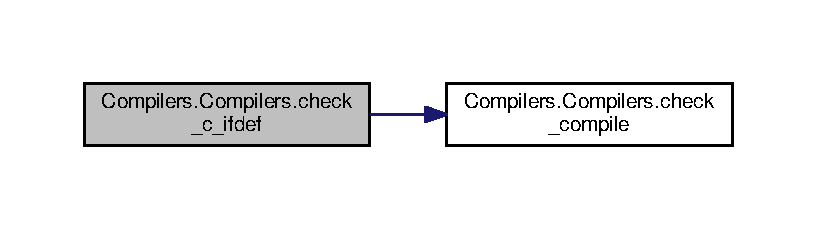
\includegraphics[width=350pt]{classCompilers_1_1Compilers_a82b789e14047fa9d8027c9df59c95dca_cgraph}
\end{center}
\end{figure}




Here is the caller graph for this function\-:
\nopagebreak
\begin{figure}[H]
\begin{center}
\leavevmode
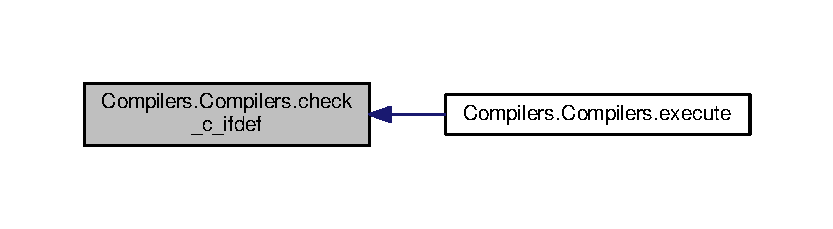
\includegraphics[width=350pt]{classCompilers_1_1Compilers_a82b789e14047fa9d8027c9df59c95dca_icgraph}
\end{center}
\end{figure}


\hypertarget{classCompilers_1_1Compilers_aac1f107915d98d9b076c68a7ebc2ec48}{\index{Compilers\-::\-Compilers@{Compilers\-::\-Compilers}!check\-\_\-compile@{check\-\_\-compile}}
\index{check\-\_\-compile@{check\-\_\-compile}!Compilers::Compilers@{Compilers\-::\-Compilers}}
\subsubsection[{check\-\_\-compile}]{\setlength{\rightskip}{0pt plus 5cm}def Compilers.\-Compilers.\-check\-\_\-compile (
\begin{DoxyParamCaption}
\item[{}]{self, }
\item[{}]{test\-Def, }
\item[{}]{macro, }
\item[{}]{c\-\_\-code, }
\item[{}]{compiler}
\end{DoxyParamCaption}
)}}\label{classCompilers_1_1Compilers_aac1f107915d98d9b076c68a7ebc2ec48}


Definition at line 174 of file Compilers.\-py.



Here is the caller graph for this function\-:
\nopagebreak
\begin{figure}[H]
\begin{center}
\leavevmode
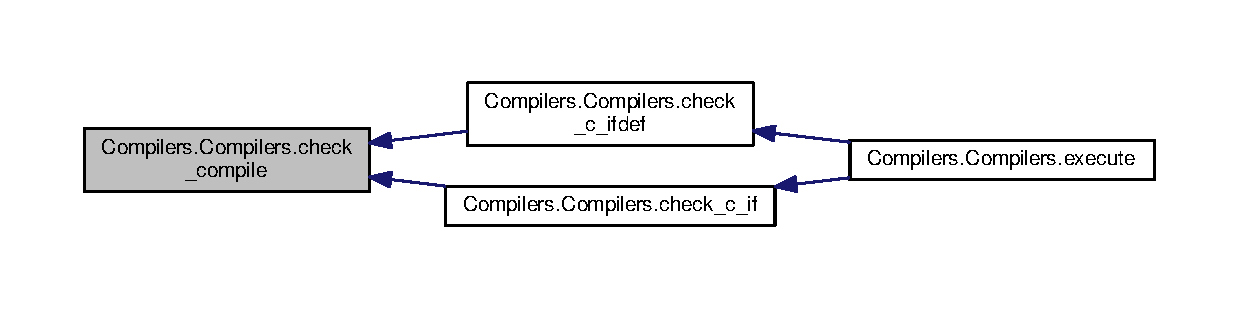
\includegraphics[width=350pt]{classCompilers_1_1Compilers_aac1f107915d98d9b076c68a7ebc2ec48_icgraph}
\end{center}
\end{figure}


\hypertarget{classCompilers_1_1Compilers_a3a65f6da74cda8747cfc7af58ad2e1ee}{\index{Compilers\-::\-Compilers@{Compilers\-::\-Compilers}!check\-\_\-version@{check\-\_\-version}}
\index{check\-\_\-version@{check\-\_\-version}!Compilers::Compilers@{Compilers\-::\-Compilers}}
\subsubsection[{check\-\_\-version}]{\setlength{\rightskip}{0pt plus 5cm}def Compilers.\-Compilers.\-check\-\_\-version (
\begin{DoxyParamCaption}
\item[{}]{self, }
\item[{}]{compiler, }
\item[{}]{version, }
\item[{}]{test\-Def}
\end{DoxyParamCaption}
)}}\label{classCompilers_1_1Compilers_a3a65f6da74cda8747cfc7af58ad2e1ee}


Definition at line 214 of file Compilers.\-py.



Here is the caller graph for this function\-:
\nopagebreak
\begin{figure}[H]
\begin{center}
\leavevmode
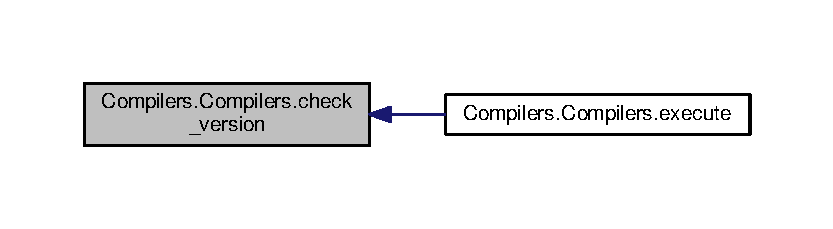
\includegraphics[width=350pt]{classCompilers_1_1Compilers_a3a65f6da74cda8747cfc7af58ad2e1ee_icgraph}
\end{center}
\end{figure}


\hypertarget{classCompilers_1_1Compilers_a85044d54e6b66cb5f29328a75f5bf446}{\index{Compilers\-::\-Compilers@{Compilers\-::\-Compilers}!execute@{execute}}
\index{execute@{execute}!Compilers::Compilers@{Compilers\-::\-Compilers}}
\subsubsection[{execute}]{\setlength{\rightskip}{0pt plus 5cm}def Compilers.\-Compilers.\-execute (
\begin{DoxyParamCaption}
\item[{}]{self, }
\item[{}]{log, }
\item[{}]{test\-Def}
\end{DoxyParamCaption}
)}}\label{classCompilers_1_1Compilers_a85044d54e6b66cb5f29328a75f5bf446}


Definition at line 34 of file Compilers.\-py.



Here is the call graph for this function\-:
\nopagebreak
\begin{figure}[H]
\begin{center}
\leavevmode
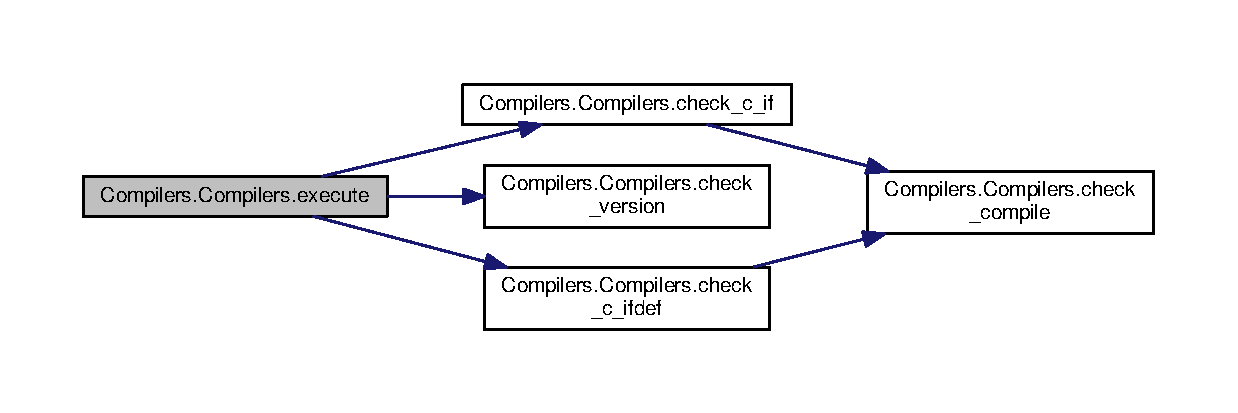
\includegraphics[width=350pt]{classCompilers_1_1Compilers_a85044d54e6b66cb5f29328a75f5bf446_cgraph}
\end{center}
\end{figure}


\hypertarget{classCompilers_1_1Compilers_aabd91a4eeb39804bbddba7c5bb1b6ec0}{\index{Compilers\-::\-Compilers@{Compilers\-::\-Compilers}!print\-\_\-name@{print\-\_\-name}}
\index{print\-\_\-name@{print\-\_\-name}!Compilers::Compilers@{Compilers\-::\-Compilers}}
\subsubsection[{print\-\_\-name}]{\setlength{\rightskip}{0pt plus 5cm}def Compilers.\-Compilers.\-print\-\_\-name (
\begin{DoxyParamCaption}
\item[{}]{self}
\end{DoxyParamCaption}
)}}\label{classCompilers_1_1Compilers_aabd91a4eeb39804bbddba7c5bb1b6ec0}


Definition at line 25 of file Compilers.\-py.

\hypertarget{classCompilers_1_1Compilers_a152a2bd6caf05098ebdfd2e336c1f71b}{\index{Compilers\-::\-Compilers@{Compilers\-::\-Compilers}!print\-\_\-options@{print\-\_\-options}}
\index{print\-\_\-options@{print\-\_\-options}!Compilers::Compilers@{Compilers\-::\-Compilers}}
\subsubsection[{print\-\_\-options}]{\setlength{\rightskip}{0pt plus 5cm}def Compilers.\-Compilers.\-print\-\_\-options (
\begin{DoxyParamCaption}
\item[{}]{self, }
\item[{}]{test\-Def, }
\item[{}]{prefix}
\end{DoxyParamCaption}
)}}\label{classCompilers_1_1Compilers_a152a2bd6caf05098ebdfd2e336c1f71b}


Definition at line 28 of file Compilers.\-py.



\subsection{Member Data Documentation}
\hypertarget{classCompilers_1_1Compilers_a29d4fb86feaa70cccd5d6b8852421767}{\index{Compilers\-::\-Compilers@{Compilers\-::\-Compilers}!options@{options}}
\index{options@{options}!Compilers::Compilers@{Compilers\-::\-Compilers}}
\subsubsection[{options}]{\setlength{\rightskip}{0pt plus 5cm}Compilers.\-Compilers.\-options}}\label{classCompilers_1_1Compilers_a29d4fb86feaa70cccd5d6b8852421767}


Definition at line 22 of file Compilers.\-py.



The documentation for this class was generated from the following file\-:\begin{DoxyCompactItemize}
\item 
/home/travis/build/open-\/mpi/mtt/pylib/\-Utilities/\hyperlink{Compilers_8py}{Compilers.\-py}\end{DoxyCompactItemize}

\hypertarget{classCopytree_1_1Copytree}{\section{Copytree.\-Copytree Class Reference}
\label{classCopytree_1_1Copytree}\index{Copytree.\-Copytree@{Copytree.\-Copytree}}
}


Inheritance diagram for Copytree.\-Copytree\-:
\nopagebreak
\begin{figure}[H]
\begin{center}
\leavevmode
\includegraphics[width=236pt]{classCopytree_1_1Copytree__inherit__graph}
\end{center}
\end{figure}


Collaboration diagram for Copytree.\-Copytree\-:
\nopagebreak
\begin{figure}[H]
\begin{center}
\leavevmode
\includegraphics[width=236pt]{classCopytree_1_1Copytree__coll__graph}
\end{center}
\end{figure}
\subsection*{Public Member Functions}
\begin{DoxyCompactItemize}
\item 
def \hyperlink{classCopytree_1_1Copytree_a7dc4242e406f7418ca7e4f0c31b8c524}{\-\_\-\-\_\-init\-\_\-\-\_\-}
\item 
def \hyperlink{classCopytree_1_1Copytree_ae6dbc27735bd3bdcb0113564c50b1c1c}{print\-\_\-name}
\item 
def \hyperlink{classCopytree_1_1Copytree_a34bbcd07e83438b9ec9855065b13a397}{print\-\_\-options}
\item 
def \hyperlink{classCopytree_1_1Copytree_a567584587407c9c6027bd7026e36a366}{execute}
\end{DoxyCompactItemize}
\subsection*{Public Attributes}
\begin{DoxyCompactItemize}
\item 
\hyperlink{classCopytree_1_1Copytree_ab12d2712ffd4aba7ddd4c5ceadec153b}{options}
\end{DoxyCompactItemize}


\subsection{Detailed Description}


Definition at line 32 of file Copytree.\-py.



\subsection{Constructor \& Destructor Documentation}
\hypertarget{classCopytree_1_1Copytree_a7dc4242e406f7418ca7e4f0c31b8c524}{\index{Copytree\-::\-Copytree@{Copytree\-::\-Copytree}!\-\_\-\-\_\-init\-\_\-\-\_\-@{\-\_\-\-\_\-init\-\_\-\-\_\-}}
\index{\-\_\-\-\_\-init\-\_\-\-\_\-@{\-\_\-\-\_\-init\-\_\-\-\_\-}!Copytree::Copytree@{Copytree\-::\-Copytree}}
\subsubsection[{\-\_\-\-\_\-init\-\_\-\-\_\-}]{\setlength{\rightskip}{0pt plus 5cm}def Copytree.\-Copytree.\-\_\-\-\_\-init\-\_\-\-\_\- (
\begin{DoxyParamCaption}
\item[{}]{self}
\end{DoxyParamCaption}
)}}\label{classCopytree_1_1Copytree_a7dc4242e406f7418ca7e4f0c31b8c524}


Definition at line 33 of file Copytree.\-py.



\subsection{Member Function Documentation}
\hypertarget{classCopytree_1_1Copytree_a567584587407c9c6027bd7026e36a366}{\index{Copytree\-::\-Copytree@{Copytree\-::\-Copytree}!execute@{execute}}
\index{execute@{execute}!Copytree::Copytree@{Copytree\-::\-Copytree}}
\subsubsection[{execute}]{\setlength{\rightskip}{0pt plus 5cm}def Copytree.\-Copytree.\-execute (
\begin{DoxyParamCaption}
\item[{}]{self, }
\item[{}]{log, }
\item[{}]{keyvals, }
\item[{}]{test\-Def}
\end{DoxyParamCaption}
)}}\label{classCopytree_1_1Copytree_a567584587407c9c6027bd7026e36a366}


Definition at line 49 of file Copytree.\-py.

\hypertarget{classCopytree_1_1Copytree_ae6dbc27735bd3bdcb0113564c50b1c1c}{\index{Copytree\-::\-Copytree@{Copytree\-::\-Copytree}!print\-\_\-name@{print\-\_\-name}}
\index{print\-\_\-name@{print\-\_\-name}!Copytree::Copytree@{Copytree\-::\-Copytree}}
\subsubsection[{print\-\_\-name}]{\setlength{\rightskip}{0pt plus 5cm}def Copytree.\-Copytree.\-print\-\_\-name (
\begin{DoxyParamCaption}
\item[{}]{self}
\end{DoxyParamCaption}
)}}\label{classCopytree_1_1Copytree_ae6dbc27735bd3bdcb0113564c50b1c1c}


Definition at line 40 of file Copytree.\-py.

\hypertarget{classCopytree_1_1Copytree_a34bbcd07e83438b9ec9855065b13a397}{\index{Copytree\-::\-Copytree@{Copytree\-::\-Copytree}!print\-\_\-options@{print\-\_\-options}}
\index{print\-\_\-options@{print\-\_\-options}!Copytree::Copytree@{Copytree\-::\-Copytree}}
\subsubsection[{print\-\_\-options}]{\setlength{\rightskip}{0pt plus 5cm}def Copytree.\-Copytree.\-print\-\_\-options (
\begin{DoxyParamCaption}
\item[{}]{self, }
\item[{}]{test\-Def, }
\item[{}]{prefix}
\end{DoxyParamCaption}
)}}\label{classCopytree_1_1Copytree_a34bbcd07e83438b9ec9855065b13a397}


Definition at line 43 of file Copytree.\-py.



\subsection{Member Data Documentation}
\hypertarget{classCopytree_1_1Copytree_ab12d2712ffd4aba7ddd4c5ceadec153b}{\index{Copytree\-::\-Copytree@{Copytree\-::\-Copytree}!options@{options}}
\index{options@{options}!Copytree::Copytree@{Copytree\-::\-Copytree}}
\subsubsection[{options}]{\setlength{\rightskip}{0pt plus 5cm}Copytree.\-Copytree.\-options}}\label{classCopytree_1_1Copytree_ab12d2712ffd4aba7ddd4c5ceadec153b}


Definition at line 35 of file Copytree.\-py.



The documentation for this class was generated from the following file\-:\begin{DoxyCompactItemize}
\item 
/home/travis/build/open-\/mpi/mtt/pylib/\-Utilities/\hyperlink{Copytree_8py}{Copytree.\-py}\end{DoxyCompactItemize}

\hypertarget{classDefaultMTTDefaults_1_1DefaultMTTDefaults}{\section{Default\-M\-T\-T\-Defaults.\-Default\-M\-T\-T\-Defaults Class Reference}
\label{classDefaultMTTDefaults_1_1DefaultMTTDefaults}\index{Default\-M\-T\-T\-Defaults.\-Default\-M\-T\-T\-Defaults@{Default\-M\-T\-T\-Defaults.\-Default\-M\-T\-T\-Defaults}}
}


Inheritance diagram for Default\-M\-T\-T\-Defaults.\-Default\-M\-T\-T\-Defaults\-:
\nopagebreak
\begin{figure}[H]
\begin{center}
\leavevmode
\includegraphics[width=258pt]{classDefaultMTTDefaults_1_1DefaultMTTDefaults__inherit__graph}
\end{center}
\end{figure}


Collaboration diagram for Default\-M\-T\-T\-Defaults.\-Default\-M\-T\-T\-Defaults\-:
\nopagebreak
\begin{figure}[H]
\begin{center}
\leavevmode
\includegraphics[width=258pt]{classDefaultMTTDefaults_1_1DefaultMTTDefaults__coll__graph}
\end{center}
\end{figure}
\subsection*{Public Member Functions}
\begin{DoxyCompactItemize}
\item 
def \hyperlink{classDefaultMTTDefaults_1_1DefaultMTTDefaults_af45ae89ffdda25b5db56cc32d6f38617}{\-\_\-\-\_\-init\-\_\-\-\_\-}
\item 
def \hyperlink{classDefaultMTTDefaults_1_1DefaultMTTDefaults_ab168e4b76bd07ff868f6d8c8dcfbabcd}{activate}
\item 
def \hyperlink{classDefaultMTTDefaults_1_1DefaultMTTDefaults_abbdeb62905e733e0145243e238991e1b}{deactivate}
\item 
def \hyperlink{classDefaultMTTDefaults_1_1DefaultMTTDefaults_a39fc17ab14b57f8aeaa7df1a6b32f059}{print\-\_\-name}
\item 
def \hyperlink{classDefaultMTTDefaults_1_1DefaultMTTDefaults_aedf1031336bf735bb00dcc8d80a0bd4a}{print\-\_\-options}
\item 
def \hyperlink{classDefaultMTTDefaults_1_1DefaultMTTDefaults_a22c85638c99e8a0dcb01d31c326bfc55}{priority}
\item 
def \hyperlink{classDefaultMTTDefaults_1_1DefaultMTTDefaults_a2ccbda4994ea610724763268ab05181e}{execute}
\end{DoxyCompactItemize}
\subsection*{Public Attributes}
\begin{DoxyCompactItemize}
\item 
\hyperlink{classDefaultMTTDefaults_1_1DefaultMTTDefaults_a733e1af4da36392ce6126d79c61aba0b}{options}
\end{DoxyCompactItemize}


\subsection{Detailed Description}


Definition at line 31 of file Default\-M\-T\-T\-Defaults.\-py.



\subsection{Constructor \& Destructor Documentation}
\hypertarget{classDefaultMTTDefaults_1_1DefaultMTTDefaults_af45ae89ffdda25b5db56cc32d6f38617}{\index{Default\-M\-T\-T\-Defaults\-::\-Default\-M\-T\-T\-Defaults@{Default\-M\-T\-T\-Defaults\-::\-Default\-M\-T\-T\-Defaults}!\-\_\-\-\_\-init\-\_\-\-\_\-@{\-\_\-\-\_\-init\-\_\-\-\_\-}}
\index{\-\_\-\-\_\-init\-\_\-\-\_\-@{\-\_\-\-\_\-init\-\_\-\-\_\-}!DefaultMTTDefaults::DefaultMTTDefaults@{Default\-M\-T\-T\-Defaults\-::\-Default\-M\-T\-T\-Defaults}}
\subsubsection[{\-\_\-\-\_\-init\-\_\-\-\_\-}]{\setlength{\rightskip}{0pt plus 5cm}def Default\-M\-T\-T\-Defaults.\-Default\-M\-T\-T\-Defaults.\-\_\-\-\_\-init\-\_\-\-\_\- (
\begin{DoxyParamCaption}
\item[{}]{self}
\end{DoxyParamCaption}
)}}\label{classDefaultMTTDefaults_1_1DefaultMTTDefaults_af45ae89ffdda25b5db56cc32d6f38617}


Definition at line 33 of file Default\-M\-T\-T\-Defaults.\-py.



\subsection{Member Function Documentation}
\hypertarget{classDefaultMTTDefaults_1_1DefaultMTTDefaults_ab168e4b76bd07ff868f6d8c8dcfbabcd}{\index{Default\-M\-T\-T\-Defaults\-::\-Default\-M\-T\-T\-Defaults@{Default\-M\-T\-T\-Defaults\-::\-Default\-M\-T\-T\-Defaults}!activate@{activate}}
\index{activate@{activate}!DefaultMTTDefaults::DefaultMTTDefaults@{Default\-M\-T\-T\-Defaults\-::\-Default\-M\-T\-T\-Defaults}}
\subsubsection[{activate}]{\setlength{\rightskip}{0pt plus 5cm}def Default\-M\-T\-T\-Defaults.\-Default\-M\-T\-T\-Defaults.\-activate (
\begin{DoxyParamCaption}
\item[{}]{self}
\end{DoxyParamCaption}
)}}\label{classDefaultMTTDefaults_1_1DefaultMTTDefaults_ab168e4b76bd07ff868f6d8c8dcfbabcd}


Definition at line 49 of file Default\-M\-T\-T\-Defaults.\-py.

\hypertarget{classDefaultMTTDefaults_1_1DefaultMTTDefaults_abbdeb62905e733e0145243e238991e1b}{\index{Default\-M\-T\-T\-Defaults\-::\-Default\-M\-T\-T\-Defaults@{Default\-M\-T\-T\-Defaults\-::\-Default\-M\-T\-T\-Defaults}!deactivate@{deactivate}}
\index{deactivate@{deactivate}!DefaultMTTDefaults::DefaultMTTDefaults@{Default\-M\-T\-T\-Defaults\-::\-Default\-M\-T\-T\-Defaults}}
\subsubsection[{deactivate}]{\setlength{\rightskip}{0pt plus 5cm}def Default\-M\-T\-T\-Defaults.\-Default\-M\-T\-T\-Defaults.\-deactivate (
\begin{DoxyParamCaption}
\item[{}]{self}
\end{DoxyParamCaption}
)}}\label{classDefaultMTTDefaults_1_1DefaultMTTDefaults_abbdeb62905e733e0145243e238991e1b}


Definition at line 55 of file Default\-M\-T\-T\-Defaults.\-py.

\hypertarget{classDefaultMTTDefaults_1_1DefaultMTTDefaults_a2ccbda4994ea610724763268ab05181e}{\index{Default\-M\-T\-T\-Defaults\-::\-Default\-M\-T\-T\-Defaults@{Default\-M\-T\-T\-Defaults\-::\-Default\-M\-T\-T\-Defaults}!execute@{execute}}
\index{execute@{execute}!DefaultMTTDefaults::DefaultMTTDefaults@{Default\-M\-T\-T\-Defaults\-::\-Default\-M\-T\-T\-Defaults}}
\subsubsection[{execute}]{\setlength{\rightskip}{0pt plus 5cm}def Default\-M\-T\-T\-Defaults.\-Default\-M\-T\-T\-Defaults.\-execute (
\begin{DoxyParamCaption}
\item[{}]{self, }
\item[{}]{log, }
\item[{}]{keyvals, }
\item[{}]{test\-Def}
\end{DoxyParamCaption}
)}}\label{classDefaultMTTDefaults_1_1DefaultMTTDefaults_a2ccbda4994ea610724763268ab05181e}


Definition at line 71 of file Default\-M\-T\-T\-Defaults.\-py.

\hypertarget{classDefaultMTTDefaults_1_1DefaultMTTDefaults_a39fc17ab14b57f8aeaa7df1a6b32f059}{\index{Default\-M\-T\-T\-Defaults\-::\-Default\-M\-T\-T\-Defaults@{Default\-M\-T\-T\-Defaults\-::\-Default\-M\-T\-T\-Defaults}!print\-\_\-name@{print\-\_\-name}}
\index{print\-\_\-name@{print\-\_\-name}!DefaultMTTDefaults::DefaultMTTDefaults@{Default\-M\-T\-T\-Defaults\-::\-Default\-M\-T\-T\-Defaults}}
\subsubsection[{print\-\_\-name}]{\setlength{\rightskip}{0pt plus 5cm}def Default\-M\-T\-T\-Defaults.\-Default\-M\-T\-T\-Defaults.\-print\-\_\-name (
\begin{DoxyParamCaption}
\item[{}]{self}
\end{DoxyParamCaption}
)}}\label{classDefaultMTTDefaults_1_1DefaultMTTDefaults_a39fc17ab14b57f8aeaa7df1a6b32f059}


Definition at line 59 of file Default\-M\-T\-T\-Defaults.\-py.

\hypertarget{classDefaultMTTDefaults_1_1DefaultMTTDefaults_aedf1031336bf735bb00dcc8d80a0bd4a}{\index{Default\-M\-T\-T\-Defaults\-::\-Default\-M\-T\-T\-Defaults@{Default\-M\-T\-T\-Defaults\-::\-Default\-M\-T\-T\-Defaults}!print\-\_\-options@{print\-\_\-options}}
\index{print\-\_\-options@{print\-\_\-options}!DefaultMTTDefaults::DefaultMTTDefaults@{Default\-M\-T\-T\-Defaults\-::\-Default\-M\-T\-T\-Defaults}}
\subsubsection[{print\-\_\-options}]{\setlength{\rightskip}{0pt plus 5cm}def Default\-M\-T\-T\-Defaults.\-Default\-M\-T\-T\-Defaults.\-print\-\_\-options (
\begin{DoxyParamCaption}
\item[{}]{self, }
\item[{}]{test\-Def, }
\item[{}]{prefix}
\end{DoxyParamCaption}
)}}\label{classDefaultMTTDefaults_1_1DefaultMTTDefaults_aedf1031336bf735bb00dcc8d80a0bd4a}


Definition at line 62 of file Default\-M\-T\-T\-Defaults.\-py.

\hypertarget{classDefaultMTTDefaults_1_1DefaultMTTDefaults_a22c85638c99e8a0dcb01d31c326bfc55}{\index{Default\-M\-T\-T\-Defaults\-::\-Default\-M\-T\-T\-Defaults@{Default\-M\-T\-T\-Defaults\-::\-Default\-M\-T\-T\-Defaults}!priority@{priority}}
\index{priority@{priority}!DefaultMTTDefaults::DefaultMTTDefaults@{Default\-M\-T\-T\-Defaults\-::\-Default\-M\-T\-T\-Defaults}}
\subsubsection[{priority}]{\setlength{\rightskip}{0pt plus 5cm}def Default\-M\-T\-T\-Defaults.\-Default\-M\-T\-T\-Defaults.\-priority (
\begin{DoxyParamCaption}
\item[{}]{self}
\end{DoxyParamCaption}
)}}\label{classDefaultMTTDefaults_1_1DefaultMTTDefaults_a22c85638c99e8a0dcb01d31c326bfc55}


Definition at line 68 of file Default\-M\-T\-T\-Defaults.\-py.



\subsection{Member Data Documentation}
\hypertarget{classDefaultMTTDefaults_1_1DefaultMTTDefaults_a733e1af4da36392ce6126d79c61aba0b}{\index{Default\-M\-T\-T\-Defaults\-::\-Default\-M\-T\-T\-Defaults@{Default\-M\-T\-T\-Defaults\-::\-Default\-M\-T\-T\-Defaults}!options@{options}}
\index{options@{options}!DefaultMTTDefaults::DefaultMTTDefaults@{Default\-M\-T\-T\-Defaults\-::\-Default\-M\-T\-T\-Defaults}}
\subsubsection[{options}]{\setlength{\rightskip}{0pt plus 5cm}Default\-M\-T\-T\-Defaults.\-Default\-M\-T\-T\-Defaults.\-options}}\label{classDefaultMTTDefaults_1_1DefaultMTTDefaults_a733e1af4da36392ce6126d79c61aba0b}


Definition at line 36 of file Default\-M\-T\-T\-Defaults.\-py.



The documentation for this class was generated from the following file\-:\begin{DoxyCompactItemize}
\item 
/home/travis/build/open-\/mpi/mtt/pylib/\-Stages/\-M\-T\-T\-Defaults/\hyperlink{DefaultMTTDefaults_8py}{Default\-M\-T\-T\-Defaults.\-py}\end{DoxyCompactItemize}

\hypertarget{classDefaultProfile_1_1DefaultProfile}{\section{Default\-Profile.\-Default\-Profile Class Reference}
\label{classDefaultProfile_1_1DefaultProfile}\index{Default\-Profile.\-Default\-Profile@{Default\-Profile.\-Default\-Profile}}
}


Inheritance diagram for Default\-Profile.\-Default\-Profile\-:
\nopagebreak
\begin{figure}[H]
\begin{center}
\leavevmode
\includegraphics[width=246pt]{classDefaultProfile_1_1DefaultProfile__inherit__graph}
\end{center}
\end{figure}


Collaboration diagram for Default\-Profile.\-Default\-Profile\-:
\nopagebreak
\begin{figure}[H]
\begin{center}
\leavevmode
\includegraphics[width=246pt]{classDefaultProfile_1_1DefaultProfile__coll__graph}
\end{center}
\end{figure}
\subsection*{Public Member Functions}
\begin{DoxyCompactItemize}
\item 
def \hyperlink{classDefaultProfile_1_1DefaultProfile_a7949e8f2a3632585e38d952b43afd205}{\-\_\-\-\_\-init\-\_\-\-\_\-}
\item 
def \hyperlink{classDefaultProfile_1_1DefaultProfile_a03edede0b46fe544777421da40d7d628}{activate}
\item 
def \hyperlink{classDefaultProfile_1_1DefaultProfile_ad9bcbf0a5b927314bcba17f4f143cbc2}{deactivate}
\item 
def \hyperlink{classDefaultProfile_1_1DefaultProfile_a74a0484b938f567fc3337f9bdd68b68a}{print\-\_\-name}
\item 
def \hyperlink{classDefaultProfile_1_1DefaultProfile_a4267f84edfc874a41a7f0558d51f4086}{print\-\_\-options}
\item 
def \hyperlink{classDefaultProfile_1_1DefaultProfile_a83a3eb62e7f08a18eb6b783f73f1d68b}{execute}
\end{DoxyCompactItemize}
\subsection*{Public Attributes}
\begin{DoxyCompactItemize}
\item 
\hyperlink{classDefaultProfile_1_1DefaultProfile_ad8d29967f62501f4638fe09ee7686d08}{options}
\end{DoxyCompactItemize}


\subsection{Detailed Description}


Definition at line 27 of file Default\-Profile.\-py.



\subsection{Constructor \& Destructor Documentation}
\hypertarget{classDefaultProfile_1_1DefaultProfile_a7949e8f2a3632585e38d952b43afd205}{\index{Default\-Profile\-::\-Default\-Profile@{Default\-Profile\-::\-Default\-Profile}!\-\_\-\-\_\-init\-\_\-\-\_\-@{\-\_\-\-\_\-init\-\_\-\-\_\-}}
\index{\-\_\-\-\_\-init\-\_\-\-\_\-@{\-\_\-\-\_\-init\-\_\-\-\_\-}!DefaultProfile::DefaultProfile@{Default\-Profile\-::\-Default\-Profile}}
\subsubsection[{\-\_\-\-\_\-init\-\_\-\-\_\-}]{\setlength{\rightskip}{0pt plus 5cm}def Default\-Profile.\-Default\-Profile.\-\_\-\-\_\-init\-\_\-\-\_\- (
\begin{DoxyParamCaption}
\item[{}]{self}
\end{DoxyParamCaption}
)}}\label{classDefaultProfile_1_1DefaultProfile_a7949e8f2a3632585e38d952b43afd205}


Definition at line 29 of file Default\-Profile.\-py.



\subsection{Member Function Documentation}
\hypertarget{classDefaultProfile_1_1DefaultProfile_a03edede0b46fe544777421da40d7d628}{\index{Default\-Profile\-::\-Default\-Profile@{Default\-Profile\-::\-Default\-Profile}!activate@{activate}}
\index{activate@{activate}!DefaultProfile::DefaultProfile@{Default\-Profile\-::\-Default\-Profile}}
\subsubsection[{activate}]{\setlength{\rightskip}{0pt plus 5cm}def Default\-Profile.\-Default\-Profile.\-activate (
\begin{DoxyParamCaption}
\item[{}]{self}
\end{DoxyParamCaption}
)}}\label{classDefaultProfile_1_1DefaultProfile_a03edede0b46fe544777421da40d7d628}


Definition at line 41 of file Default\-Profile.\-py.

\hypertarget{classDefaultProfile_1_1DefaultProfile_ad9bcbf0a5b927314bcba17f4f143cbc2}{\index{Default\-Profile\-::\-Default\-Profile@{Default\-Profile\-::\-Default\-Profile}!deactivate@{deactivate}}
\index{deactivate@{deactivate}!DefaultProfile::DefaultProfile@{Default\-Profile\-::\-Default\-Profile}}
\subsubsection[{deactivate}]{\setlength{\rightskip}{0pt plus 5cm}def Default\-Profile.\-Default\-Profile.\-deactivate (
\begin{DoxyParamCaption}
\item[{}]{self}
\end{DoxyParamCaption}
)}}\label{classDefaultProfile_1_1DefaultProfile_ad9bcbf0a5b927314bcba17f4f143cbc2}


Definition at line 47 of file Default\-Profile.\-py.

\hypertarget{classDefaultProfile_1_1DefaultProfile_a83a3eb62e7f08a18eb6b783f73f1d68b}{\index{Default\-Profile\-::\-Default\-Profile@{Default\-Profile\-::\-Default\-Profile}!execute@{execute}}
\index{execute@{execute}!DefaultProfile::DefaultProfile@{Default\-Profile\-::\-Default\-Profile}}
\subsubsection[{execute}]{\setlength{\rightskip}{0pt plus 5cm}def Default\-Profile.\-Default\-Profile.\-execute (
\begin{DoxyParamCaption}
\item[{}]{self, }
\item[{}]{log, }
\item[{}]{keyvals, }
\item[{}]{test\-Def}
\end{DoxyParamCaption}
)}}\label{classDefaultProfile_1_1DefaultProfile_a83a3eb62e7f08a18eb6b783f73f1d68b}


Definition at line 60 of file Default\-Profile.\-py.

\hypertarget{classDefaultProfile_1_1DefaultProfile_a74a0484b938f567fc3337f9bdd68b68a}{\index{Default\-Profile\-::\-Default\-Profile@{Default\-Profile\-::\-Default\-Profile}!print\-\_\-name@{print\-\_\-name}}
\index{print\-\_\-name@{print\-\_\-name}!DefaultProfile::DefaultProfile@{Default\-Profile\-::\-Default\-Profile}}
\subsubsection[{print\-\_\-name}]{\setlength{\rightskip}{0pt plus 5cm}def Default\-Profile.\-Default\-Profile.\-print\-\_\-name (
\begin{DoxyParamCaption}
\item[{}]{self}
\end{DoxyParamCaption}
)}}\label{classDefaultProfile_1_1DefaultProfile_a74a0484b938f567fc3337f9bdd68b68a}


Definition at line 51 of file Default\-Profile.\-py.

\hypertarget{classDefaultProfile_1_1DefaultProfile_a4267f84edfc874a41a7f0558d51f4086}{\index{Default\-Profile\-::\-Default\-Profile@{Default\-Profile\-::\-Default\-Profile}!print\-\_\-options@{print\-\_\-options}}
\index{print\-\_\-options@{print\-\_\-options}!DefaultProfile::DefaultProfile@{Default\-Profile\-::\-Default\-Profile}}
\subsubsection[{print\-\_\-options}]{\setlength{\rightskip}{0pt plus 5cm}def Default\-Profile.\-Default\-Profile.\-print\-\_\-options (
\begin{DoxyParamCaption}
\item[{}]{self, }
\item[{}]{test\-Def, }
\item[{}]{prefix}
\end{DoxyParamCaption}
)}}\label{classDefaultProfile_1_1DefaultProfile_a4267f84edfc874a41a7f0558d51f4086}


Definition at line 54 of file Default\-Profile.\-py.



\subsection{Member Data Documentation}
\hypertarget{classDefaultProfile_1_1DefaultProfile_ad8d29967f62501f4638fe09ee7686d08}{\index{Default\-Profile\-::\-Default\-Profile@{Default\-Profile\-::\-Default\-Profile}!options@{options}}
\index{options@{options}!DefaultProfile::DefaultProfile@{Default\-Profile\-::\-Default\-Profile}}
\subsubsection[{options}]{\setlength{\rightskip}{0pt plus 5cm}Default\-Profile.\-Default\-Profile.\-options}}\label{classDefaultProfile_1_1DefaultProfile_ad8d29967f62501f4638fe09ee7686d08}


Definition at line 32 of file Default\-Profile.\-py.



The documentation for this class was generated from the following file\-:\begin{DoxyCompactItemize}
\item 
/home/travis/build/open-\/mpi/mtt/pylib/\-Stages/\-Profile/\hyperlink{DefaultProfile_8py}{Default\-Profile.\-py}\end{DoxyCompactItemize}

\hypertarget{classDefaultTestBuild_1_1DefaultTestBuild}{\section{Default\-Test\-Build.\-Default\-Test\-Build Class Reference}
\label{classDefaultTestBuild_1_1DefaultTestBuild}\index{Default\-Test\-Build.\-Default\-Test\-Build@{Default\-Test\-Build.\-Default\-Test\-Build}}
}


Inheritance diagram for Default\-Test\-Build.\-Default\-Test\-Build\-:
\nopagebreak
\begin{figure}[H]
\begin{center}
\leavevmode
\includegraphics[width=228pt]{classDefaultTestBuild_1_1DefaultTestBuild__inherit__graph}
\end{center}
\end{figure}


Collaboration diagram for Default\-Test\-Build.\-Default\-Test\-Build\-:
\nopagebreak
\begin{figure}[H]
\begin{center}
\leavevmode
\includegraphics[width=228pt]{classDefaultTestBuild_1_1DefaultTestBuild__coll__graph}
\end{center}
\end{figure}
\subsection*{Public Member Functions}
\begin{DoxyCompactItemize}
\item 
def \hyperlink{classDefaultTestBuild_1_1DefaultTestBuild_a08729e27591861a8c9b61a6b2618ec2f}{\-\_\-\-\_\-init\-\_\-\-\_\-}
\item 
def \hyperlink{classDefaultTestBuild_1_1DefaultTestBuild_a88b530e5d66e5dc310f77087d8744345}{activate}
\item 
def \hyperlink{classDefaultTestBuild_1_1DefaultTestBuild_a3a1fbc64d9a4750d7ecf722fb6bcd1ce}{deactivate}
\item 
def \hyperlink{classDefaultTestBuild_1_1DefaultTestBuild_a391c37a5d652ad857c57ae07b66b0d7e}{print\-\_\-name}
\item 
def \hyperlink{classDefaultTestBuild_1_1DefaultTestBuild_a38238916f0726d3a8e2b352ddc74f424}{print\-\_\-options}
\item 
def \hyperlink{classDefaultTestBuild_1_1DefaultTestBuild_a17ce5f679320871748b5aa3ea3491c28}{execute}
\end{DoxyCompactItemize}
\subsection*{Public Attributes}
\begin{DoxyCompactItemize}
\item 
\hyperlink{classDefaultTestBuild_1_1DefaultTestBuild_a2c22896be00540cc15625e79bc98c9fc}{options}
\end{DoxyCompactItemize}


\subsection{Detailed Description}


Definition at line 28 of file Default\-Test\-Build.\-py.



\subsection{Constructor \& Destructor Documentation}
\hypertarget{classDefaultTestBuild_1_1DefaultTestBuild_a08729e27591861a8c9b61a6b2618ec2f}{\index{Default\-Test\-Build\-::\-Default\-Test\-Build@{Default\-Test\-Build\-::\-Default\-Test\-Build}!\-\_\-\-\_\-init\-\_\-\-\_\-@{\-\_\-\-\_\-init\-\_\-\-\_\-}}
\index{\-\_\-\-\_\-init\-\_\-\-\_\-@{\-\_\-\-\_\-init\-\_\-\-\_\-}!DefaultTestBuild::DefaultTestBuild@{Default\-Test\-Build\-::\-Default\-Test\-Build}}
\subsubsection[{\-\_\-\-\_\-init\-\_\-\-\_\-}]{\setlength{\rightskip}{0pt plus 5cm}def Default\-Test\-Build.\-Default\-Test\-Build.\-\_\-\-\_\-init\-\_\-\-\_\- (
\begin{DoxyParamCaption}
\item[{}]{self}
\end{DoxyParamCaption}
)}}\label{classDefaultTestBuild_1_1DefaultTestBuild_a08729e27591861a8c9b61a6b2618ec2f}


Definition at line 30 of file Default\-Test\-Build.\-py.



\subsection{Member Function Documentation}
\hypertarget{classDefaultTestBuild_1_1DefaultTestBuild_a88b530e5d66e5dc310f77087d8744345}{\index{Default\-Test\-Build\-::\-Default\-Test\-Build@{Default\-Test\-Build\-::\-Default\-Test\-Build}!activate@{activate}}
\index{activate@{activate}!DefaultTestBuild::DefaultTestBuild@{Default\-Test\-Build\-::\-Default\-Test\-Build}}
\subsubsection[{activate}]{\setlength{\rightskip}{0pt plus 5cm}def Default\-Test\-Build.\-Default\-Test\-Build.\-activate (
\begin{DoxyParamCaption}
\item[{}]{self}
\end{DoxyParamCaption}
)}}\label{classDefaultTestBuild_1_1DefaultTestBuild_a88b530e5d66e5dc310f77087d8744345}


Definition at line 43 of file Default\-Test\-Build.\-py.

\hypertarget{classDefaultTestBuild_1_1DefaultTestBuild_a3a1fbc64d9a4750d7ecf722fb6bcd1ce}{\index{Default\-Test\-Build\-::\-Default\-Test\-Build@{Default\-Test\-Build\-::\-Default\-Test\-Build}!deactivate@{deactivate}}
\index{deactivate@{deactivate}!DefaultTestBuild::DefaultTestBuild@{Default\-Test\-Build\-::\-Default\-Test\-Build}}
\subsubsection[{deactivate}]{\setlength{\rightskip}{0pt plus 5cm}def Default\-Test\-Build.\-Default\-Test\-Build.\-deactivate (
\begin{DoxyParamCaption}
\item[{}]{self}
\end{DoxyParamCaption}
)}}\label{classDefaultTestBuild_1_1DefaultTestBuild_a3a1fbc64d9a4750d7ecf722fb6bcd1ce}


Definition at line 49 of file Default\-Test\-Build.\-py.

\hypertarget{classDefaultTestBuild_1_1DefaultTestBuild_a17ce5f679320871748b5aa3ea3491c28}{\index{Default\-Test\-Build\-::\-Default\-Test\-Build@{Default\-Test\-Build\-::\-Default\-Test\-Build}!execute@{execute}}
\index{execute@{execute}!DefaultTestBuild::DefaultTestBuild@{Default\-Test\-Build\-::\-Default\-Test\-Build}}
\subsubsection[{execute}]{\setlength{\rightskip}{0pt plus 5cm}def Default\-Test\-Build.\-Default\-Test\-Build.\-execute (
\begin{DoxyParamCaption}
\item[{}]{self, }
\item[{}]{log, }
\item[{}]{keyvals, }
\item[{}]{test\-Def}
\end{DoxyParamCaption}
)}}\label{classDefaultTestBuild_1_1DefaultTestBuild_a17ce5f679320871748b5aa3ea3491c28}


Definition at line 62 of file Default\-Test\-Build.\-py.

\hypertarget{classDefaultTestBuild_1_1DefaultTestBuild_a391c37a5d652ad857c57ae07b66b0d7e}{\index{Default\-Test\-Build\-::\-Default\-Test\-Build@{Default\-Test\-Build\-::\-Default\-Test\-Build}!print\-\_\-name@{print\-\_\-name}}
\index{print\-\_\-name@{print\-\_\-name}!DefaultTestBuild::DefaultTestBuild@{Default\-Test\-Build\-::\-Default\-Test\-Build}}
\subsubsection[{print\-\_\-name}]{\setlength{\rightskip}{0pt plus 5cm}def Default\-Test\-Build.\-Default\-Test\-Build.\-print\-\_\-name (
\begin{DoxyParamCaption}
\item[{}]{self}
\end{DoxyParamCaption}
)}}\label{classDefaultTestBuild_1_1DefaultTestBuild_a391c37a5d652ad857c57ae07b66b0d7e}


Definition at line 53 of file Default\-Test\-Build.\-py.

\hypertarget{classDefaultTestBuild_1_1DefaultTestBuild_a38238916f0726d3a8e2b352ddc74f424}{\index{Default\-Test\-Build\-::\-Default\-Test\-Build@{Default\-Test\-Build\-::\-Default\-Test\-Build}!print\-\_\-options@{print\-\_\-options}}
\index{print\-\_\-options@{print\-\_\-options}!DefaultTestBuild::DefaultTestBuild@{Default\-Test\-Build\-::\-Default\-Test\-Build}}
\subsubsection[{print\-\_\-options}]{\setlength{\rightskip}{0pt plus 5cm}def Default\-Test\-Build.\-Default\-Test\-Build.\-print\-\_\-options (
\begin{DoxyParamCaption}
\item[{}]{self, }
\item[{}]{test\-Def, }
\item[{}]{prefix}
\end{DoxyParamCaption}
)}}\label{classDefaultTestBuild_1_1DefaultTestBuild_a38238916f0726d3a8e2b352ddc74f424}


Definition at line 56 of file Default\-Test\-Build.\-py.



\subsection{Member Data Documentation}
\hypertarget{classDefaultTestBuild_1_1DefaultTestBuild_a2c22896be00540cc15625e79bc98c9fc}{\index{Default\-Test\-Build\-::\-Default\-Test\-Build@{Default\-Test\-Build\-::\-Default\-Test\-Build}!options@{options}}
\index{options@{options}!DefaultTestBuild::DefaultTestBuild@{Default\-Test\-Build\-::\-Default\-Test\-Build}}
\subsubsection[{options}]{\setlength{\rightskip}{0pt plus 5cm}Default\-Test\-Build.\-Default\-Test\-Build.\-options}}\label{classDefaultTestBuild_1_1DefaultTestBuild_a2c22896be00540cc15625e79bc98c9fc}


Definition at line 33 of file Default\-Test\-Build.\-py.



The documentation for this class was generated from the following file\-:\begin{DoxyCompactItemize}
\item 
/home/travis/build/open-\/mpi/mtt/pylib/\-Stages/\-Test\-Build/\hyperlink{DefaultTestBuild_8py}{Default\-Test\-Build.\-py}\end{DoxyCompactItemize}

\hypertarget{classEnviron_1_1Environ}{\section{Environ.\-Environ Class Reference}
\label{classEnviron_1_1Environ}\index{Environ.\-Environ@{Environ.\-Environ}}
}


Inheritance diagram for Environ.\-Environ\-:
\nopagebreak
\begin{figure}[H]
\begin{center}
\leavevmode
\includegraphics[width=236pt]{classEnviron_1_1Environ__inherit__graph}
\end{center}
\end{figure}


Collaboration diagram for Environ.\-Environ\-:
\nopagebreak
\begin{figure}[H]
\begin{center}
\leavevmode
\includegraphics[width=236pt]{classEnviron_1_1Environ__coll__graph}
\end{center}
\end{figure}
\subsection*{Public Member Functions}
\begin{DoxyCompactItemize}
\item 
def \hyperlink{classEnviron_1_1Environ_a298b6da7e53ae9d91fb2d2e6cba89a99}{\-\_\-\-\_\-init\-\_\-\-\_\-}
\item 
def \hyperlink{classEnviron_1_1Environ_a2a24fc03046a5b025df86c5ae1dc69ba}{print\-\_\-name}
\item 
def \hyperlink{classEnviron_1_1Environ_a91417cf853ffd5ef54e8b929a53c44ad}{print\-\_\-options}
\item 
def \hyperlink{classEnviron_1_1Environ_a1f0a93524611bcd9958a6995970eb2dc}{execute}
\end{DoxyCompactItemize}
\subsection*{Public Attributes}
\begin{DoxyCompactItemize}
\item 
\hyperlink{classEnviron_1_1Environ_a9e1a6482623e5f36b1de334c27df5011}{options}
\end{DoxyCompactItemize}


\subsection{Detailed Description}


Definition at line 20 of file Environ.\-py.



\subsection{Constructor \& Destructor Documentation}
\hypertarget{classEnviron_1_1Environ_a298b6da7e53ae9d91fb2d2e6cba89a99}{\index{Environ\-::\-Environ@{Environ\-::\-Environ}!\-\_\-\-\_\-init\-\_\-\-\_\-@{\-\_\-\-\_\-init\-\_\-\-\_\-}}
\index{\-\_\-\-\_\-init\-\_\-\-\_\-@{\-\_\-\-\_\-init\-\_\-\-\_\-}!Environ::Environ@{Environ\-::\-Environ}}
\subsubsection[{\-\_\-\-\_\-init\-\_\-\-\_\-}]{\setlength{\rightskip}{0pt plus 5cm}def Environ.\-Environ.\-\_\-\-\_\-init\-\_\-\-\_\- (
\begin{DoxyParamCaption}
\item[{}]{self}
\end{DoxyParamCaption}
)}}\label{classEnviron_1_1Environ_a298b6da7e53ae9d91fb2d2e6cba89a99}


Definition at line 21 of file Environ.\-py.



\subsection{Member Function Documentation}
\hypertarget{classEnviron_1_1Environ_a1f0a93524611bcd9958a6995970eb2dc}{\index{Environ\-::\-Environ@{Environ\-::\-Environ}!execute@{execute}}
\index{execute@{execute}!Environ::Environ@{Environ\-::\-Environ}}
\subsubsection[{execute}]{\setlength{\rightskip}{0pt plus 5cm}def Environ.\-Environ.\-execute (
\begin{DoxyParamCaption}
\item[{}]{self, }
\item[{}]{log, }
\item[{}]{keyvals, }
\item[{}]{test\-Def}
\end{DoxyParamCaption}
)}}\label{classEnviron_1_1Environ_a1f0a93524611bcd9958a6995970eb2dc}


Definition at line 34 of file Environ.\-py.

\hypertarget{classEnviron_1_1Environ_a2a24fc03046a5b025df86c5ae1dc69ba}{\index{Environ\-::\-Environ@{Environ\-::\-Environ}!print\-\_\-name@{print\-\_\-name}}
\index{print\-\_\-name@{print\-\_\-name}!Environ::Environ@{Environ\-::\-Environ}}
\subsubsection[{print\-\_\-name}]{\setlength{\rightskip}{0pt plus 5cm}def Environ.\-Environ.\-print\-\_\-name (
\begin{DoxyParamCaption}
\item[{}]{self}
\end{DoxyParamCaption}
)}}\label{classEnviron_1_1Environ_a2a24fc03046a5b025df86c5ae1dc69ba}


Definition at line 25 of file Environ.\-py.

\hypertarget{classEnviron_1_1Environ_a91417cf853ffd5ef54e8b929a53c44ad}{\index{Environ\-::\-Environ@{Environ\-::\-Environ}!print\-\_\-options@{print\-\_\-options}}
\index{print\-\_\-options@{print\-\_\-options}!Environ::Environ@{Environ\-::\-Environ}}
\subsubsection[{print\-\_\-options}]{\setlength{\rightskip}{0pt plus 5cm}def Environ.\-Environ.\-print\-\_\-options (
\begin{DoxyParamCaption}
\item[{}]{self, }
\item[{}]{test\-Def, }
\item[{}]{prefix}
\end{DoxyParamCaption}
)}}\label{classEnviron_1_1Environ_a91417cf853ffd5ef54e8b929a53c44ad}


Definition at line 28 of file Environ.\-py.



\subsection{Member Data Documentation}
\hypertarget{classEnviron_1_1Environ_a9e1a6482623e5f36b1de334c27df5011}{\index{Environ\-::\-Environ@{Environ\-::\-Environ}!options@{options}}
\index{options@{options}!Environ::Environ@{Environ\-::\-Environ}}
\subsubsection[{options}]{\setlength{\rightskip}{0pt plus 5cm}Environ.\-Environ.\-options}}\label{classEnviron_1_1Environ_a9e1a6482623e5f36b1de334c27df5011}


Definition at line 23 of file Environ.\-py.



The documentation for this class was generated from the following file\-:\begin{DoxyCompactItemize}
\item 
/home/travis/build/open-\/mpi/mtt/pylib/\-Utilities/\hyperlink{Environ_8py}{Environ.\-py}\end{DoxyCompactItemize}

\hypertarget{classExecuteCmd_1_1ExecuteCmd}{\section{Execute\-Cmd.\-Execute\-Cmd Class Reference}
\label{classExecuteCmd_1_1ExecuteCmd}\index{Execute\-Cmd.\-Execute\-Cmd@{Execute\-Cmd.\-Execute\-Cmd}}
}


Inheritance diagram for Execute\-Cmd.\-Execute\-Cmd\-:
\nopagebreak
\begin{figure}[H]
\begin{center}
\leavevmode
\includegraphics[width=236pt]{classExecuteCmd_1_1ExecuteCmd__inherit__graph}
\end{center}
\end{figure}


Collaboration diagram for Execute\-Cmd.\-Execute\-Cmd\-:
\nopagebreak
\begin{figure}[H]
\begin{center}
\leavevmode
\includegraphics[width=236pt]{classExecuteCmd_1_1ExecuteCmd__coll__graph}
\end{center}
\end{figure}
\subsection*{Public Member Functions}
\begin{DoxyCompactItemize}
\item 
def \hyperlink{classExecuteCmd_1_1ExecuteCmd_ae0e361beb27aac47f2c682418577b375}{\-\_\-\-\_\-init\-\_\-\-\_\-}
\item 
def \hyperlink{classExecuteCmd_1_1ExecuteCmd_a9021ad1c3f3ed4460d57d42a8d1f23ef}{print\-\_\-name}
\item 
def \hyperlink{classExecuteCmd_1_1ExecuteCmd_a8174353fba2a214e50529b2612e078ff}{print\-\_\-options}
\item 
def \hyperlink{classExecuteCmd_1_1ExecuteCmd_abd51ca569e60d044fe278b613459c709}{execute}
\end{DoxyCompactItemize}
\subsection*{Public Attributes}
\begin{DoxyCompactItemize}
\item 
\hyperlink{classExecuteCmd_1_1ExecuteCmd_aea248b8edd01b26099f3d45b798a65be}{options}
\end{DoxyCompactItemize}
\subsection*{Private Member Functions}
\begin{DoxyCompactItemize}
\item 
def \hyperlink{classExecuteCmd_1_1ExecuteCmd_a4ab1a3d66079bcb8de5a4a436282ab5c}{\-\_\-bool\-\_\-option}
\item 
def \hyperlink{classExecuteCmd_1_1ExecuteCmd_a657ac6b5c7779499ce426ba18234824e}{\-\_\-positive\-\_\-int\-\_\-option}
\end{DoxyCompactItemize}


\subsection{Detailed Description}


Definition at line 25 of file Execute\-Cmd.\-py.



\subsection{Constructor \& Destructor Documentation}
\hypertarget{classExecuteCmd_1_1ExecuteCmd_ae0e361beb27aac47f2c682418577b375}{\index{Execute\-Cmd\-::\-Execute\-Cmd@{Execute\-Cmd\-::\-Execute\-Cmd}!\-\_\-\-\_\-init\-\_\-\-\_\-@{\-\_\-\-\_\-init\-\_\-\-\_\-}}
\index{\-\_\-\-\_\-init\-\_\-\-\_\-@{\-\_\-\-\_\-init\-\_\-\-\_\-}!ExecuteCmd::ExecuteCmd@{Execute\-Cmd\-::\-Execute\-Cmd}}
\subsubsection[{\-\_\-\-\_\-init\-\_\-\-\_\-}]{\setlength{\rightskip}{0pt plus 5cm}def Execute\-Cmd.\-Execute\-Cmd.\-\_\-\-\_\-init\-\_\-\-\_\- (
\begin{DoxyParamCaption}
\item[{}]{self}
\end{DoxyParamCaption}
)}}\label{classExecuteCmd_1_1ExecuteCmd_ae0e361beb27aac47f2c682418577b375}


Definition at line 26 of file Execute\-Cmd.\-py.



\subsection{Member Function Documentation}
\hypertarget{classExecuteCmd_1_1ExecuteCmd_a4ab1a3d66079bcb8de5a4a436282ab5c}{\index{Execute\-Cmd\-::\-Execute\-Cmd@{Execute\-Cmd\-::\-Execute\-Cmd}!\-\_\-bool\-\_\-option@{\-\_\-bool\-\_\-option}}
\index{\-\_\-bool\-\_\-option@{\-\_\-bool\-\_\-option}!ExecuteCmd::ExecuteCmd@{Execute\-Cmd\-::\-Execute\-Cmd}}
\subsubsection[{\-\_\-bool\-\_\-option}]{\setlength{\rightskip}{0pt plus 5cm}def Execute\-Cmd.\-Execute\-Cmd.\-\_\-bool\-\_\-option (
\begin{DoxyParamCaption}
\item[{}]{self, }
\item[{}]{options, }
\item[{}]{name}
\end{DoxyParamCaption}
)\hspace{0.3cm}{\ttfamily [private]}}}\label{classExecuteCmd_1_1ExecuteCmd_a4ab1a3d66079bcb8de5a4a436282ab5c}


Definition at line 40 of file Execute\-Cmd.\-py.



Here is the caller graph for this function\-:
\nopagebreak
\begin{figure}[H]
\begin{center}
\leavevmode
\includegraphics[width=350pt]{classExecuteCmd_1_1ExecuteCmd_a4ab1a3d66079bcb8de5a4a436282ab5c_icgraph}
\end{center}
\end{figure}


\hypertarget{classExecuteCmd_1_1ExecuteCmd_a657ac6b5c7779499ce426ba18234824e}{\index{Execute\-Cmd\-::\-Execute\-Cmd@{Execute\-Cmd\-::\-Execute\-Cmd}!\-\_\-positive\-\_\-int\-\_\-option@{\-\_\-positive\-\_\-int\-\_\-option}}
\index{\-\_\-positive\-\_\-int\-\_\-option@{\-\_\-positive\-\_\-int\-\_\-option}!ExecuteCmd::ExecuteCmd@{Execute\-Cmd\-::\-Execute\-Cmd}}
\subsubsection[{\-\_\-positive\-\_\-int\-\_\-option}]{\setlength{\rightskip}{0pt plus 5cm}def Execute\-Cmd.\-Execute\-Cmd.\-\_\-positive\-\_\-int\-\_\-option (
\begin{DoxyParamCaption}
\item[{}]{self, }
\item[{}]{options, }
\item[{}]{name}
\end{DoxyParamCaption}
)\hspace{0.3cm}{\ttfamily [private]}}}\label{classExecuteCmd_1_1ExecuteCmd_a657ac6b5c7779499ce426ba18234824e}


Definition at line 53 of file Execute\-Cmd.\-py.



Here is the caller graph for this function\-:
\nopagebreak
\begin{figure}[H]
\begin{center}
\leavevmode
\includegraphics[width=350pt]{classExecuteCmd_1_1ExecuteCmd_a657ac6b5c7779499ce426ba18234824e_icgraph}
\end{center}
\end{figure}


\hypertarget{classExecuteCmd_1_1ExecuteCmd_abd51ca569e60d044fe278b613459c709}{\index{Execute\-Cmd\-::\-Execute\-Cmd@{Execute\-Cmd\-::\-Execute\-Cmd}!execute@{execute}}
\index{execute@{execute}!ExecuteCmd::ExecuteCmd@{Execute\-Cmd\-::\-Execute\-Cmd}}
\subsubsection[{execute}]{\setlength{\rightskip}{0pt plus 5cm}def Execute\-Cmd.\-Execute\-Cmd.\-execute (
\begin{DoxyParamCaption}
\item[{}]{self, }
\item[{}]{options, }
\item[{}]{cmdargs, }
\item[{}]{test\-Def}
\end{DoxyParamCaption}
)}}\label{classExecuteCmd_1_1ExecuteCmd_abd51ca569e60d044fe278b613459c709}


Definition at line 61 of file Execute\-Cmd.\-py.



Here is the call graph for this function\-:
\nopagebreak
\begin{figure}[H]
\begin{center}
\leavevmode
\includegraphics[width=350pt]{classExecuteCmd_1_1ExecuteCmd_abd51ca569e60d044fe278b613459c709_cgraph}
\end{center}
\end{figure}


\hypertarget{classExecuteCmd_1_1ExecuteCmd_a9021ad1c3f3ed4460d57d42a8d1f23ef}{\index{Execute\-Cmd\-::\-Execute\-Cmd@{Execute\-Cmd\-::\-Execute\-Cmd}!print\-\_\-name@{print\-\_\-name}}
\index{print\-\_\-name@{print\-\_\-name}!ExecuteCmd::ExecuteCmd@{Execute\-Cmd\-::\-Execute\-Cmd}}
\subsubsection[{print\-\_\-name}]{\setlength{\rightskip}{0pt plus 5cm}def Execute\-Cmd.\-Execute\-Cmd.\-print\-\_\-name (
\begin{DoxyParamCaption}
\item[{}]{self}
\end{DoxyParamCaption}
)}}\label{classExecuteCmd_1_1ExecuteCmd_a9021ad1c3f3ed4460d57d42a8d1f23ef}


Definition at line 31 of file Execute\-Cmd.\-py.

\hypertarget{classExecuteCmd_1_1ExecuteCmd_a8174353fba2a214e50529b2612e078ff}{\index{Execute\-Cmd\-::\-Execute\-Cmd@{Execute\-Cmd\-::\-Execute\-Cmd}!print\-\_\-options@{print\-\_\-options}}
\index{print\-\_\-options@{print\-\_\-options}!ExecuteCmd::ExecuteCmd@{Execute\-Cmd\-::\-Execute\-Cmd}}
\subsubsection[{print\-\_\-options}]{\setlength{\rightskip}{0pt plus 5cm}def Execute\-Cmd.\-Execute\-Cmd.\-print\-\_\-options (
\begin{DoxyParamCaption}
\item[{}]{self, }
\item[{}]{test\-Def, }
\item[{}]{prefix}
\end{DoxyParamCaption}
)}}\label{classExecuteCmd_1_1ExecuteCmd_a8174353fba2a214e50529b2612e078ff}


Definition at line 34 of file Execute\-Cmd.\-py.



\subsection{Member Data Documentation}
\hypertarget{classExecuteCmd_1_1ExecuteCmd_aea248b8edd01b26099f3d45b798a65be}{\index{Execute\-Cmd\-::\-Execute\-Cmd@{Execute\-Cmd\-::\-Execute\-Cmd}!options@{options}}
\index{options@{options}!ExecuteCmd::ExecuteCmd@{Execute\-Cmd\-::\-Execute\-Cmd}}
\subsubsection[{options}]{\setlength{\rightskip}{0pt plus 5cm}Execute\-Cmd.\-Execute\-Cmd.\-options}}\label{classExecuteCmd_1_1ExecuteCmd_aea248b8edd01b26099f3d45b798a65be}


Definition at line 28 of file Execute\-Cmd.\-py.



The documentation for this class was generated from the following file\-:\begin{DoxyCompactItemize}
\item 
/home/travis/build/open-\/mpi/mtt/pylib/\-Utilities/\hyperlink{ExecuteCmd_8py}{Execute\-Cmd.\-py}\end{DoxyCompactItemize}

\hypertarget{classExecutorMTTTool_1_1ExecutorMTTTool}{\section{Executor\-M\-T\-T\-Tool.\-Executor\-M\-T\-T\-Tool Class Reference}
\label{classExecutorMTTTool_1_1ExecutorMTTTool}\index{Executor\-M\-T\-T\-Tool.\-Executor\-M\-T\-T\-Tool@{Executor\-M\-T\-T\-Tool.\-Executor\-M\-T\-T\-Tool}}
}


Inheritance diagram for Executor\-M\-T\-T\-Tool.\-Executor\-M\-T\-T\-Tool\-:
\nopagebreak
\begin{figure}[H]
\begin{center}
\leavevmode
\includegraphics[width=350pt]{classExecutorMTTTool_1_1ExecutorMTTTool__inherit__graph}
\end{center}
\end{figure}


Collaboration diagram for Executor\-M\-T\-T\-Tool.\-Executor\-M\-T\-T\-Tool\-:
\nopagebreak
\begin{figure}[H]
\begin{center}
\leavevmode
\includegraphics[width=216pt]{classExecutorMTTTool_1_1ExecutorMTTTool__coll__graph}
\end{center}
\end{figure}
\subsection*{Public Member Functions}
\begin{DoxyCompactItemize}
\item 
def \hyperlink{classExecutorMTTTool_1_1ExecutorMTTTool_afe2f512bab6b4779201b91956dcd4097}{\-\_\-\-\_\-init\-\_\-\-\_\-}
\item 
def \hyperlink{classExecutorMTTTool_1_1ExecutorMTTTool_a013abcdbf3fd5b750f66cef671b06a77}{print\-\_\-name}
\end{DoxyCompactItemize}


\subsection{Detailed Description}


Definition at line 19 of file Executor\-M\-T\-T\-Tool.\-py.



\subsection{Constructor \& Destructor Documentation}
\hypertarget{classExecutorMTTTool_1_1ExecutorMTTTool_afe2f512bab6b4779201b91956dcd4097}{\index{Executor\-M\-T\-T\-Tool\-::\-Executor\-M\-T\-T\-Tool@{Executor\-M\-T\-T\-Tool\-::\-Executor\-M\-T\-T\-Tool}!\-\_\-\-\_\-init\-\_\-\-\_\-@{\-\_\-\-\_\-init\-\_\-\-\_\-}}
\index{\-\_\-\-\_\-init\-\_\-\-\_\-@{\-\_\-\-\_\-init\-\_\-\-\_\-}!ExecutorMTTTool::ExecutorMTTTool@{Executor\-M\-T\-T\-Tool\-::\-Executor\-M\-T\-T\-Tool}}
\subsubsection[{\-\_\-\-\_\-init\-\_\-\-\_\-}]{\setlength{\rightskip}{0pt plus 5cm}def Executor\-M\-T\-T\-Tool.\-Executor\-M\-T\-T\-Tool.\-\_\-\-\_\-init\-\_\-\-\_\- (
\begin{DoxyParamCaption}
\item[{}]{self}
\end{DoxyParamCaption}
)}}\label{classExecutorMTTTool_1_1ExecutorMTTTool_afe2f512bab6b4779201b91956dcd4097}


Definition at line 20 of file Executor\-M\-T\-T\-Tool.\-py.



\subsection{Member Function Documentation}
\hypertarget{classExecutorMTTTool_1_1ExecutorMTTTool_a013abcdbf3fd5b750f66cef671b06a77}{\index{Executor\-M\-T\-T\-Tool\-::\-Executor\-M\-T\-T\-Tool@{Executor\-M\-T\-T\-Tool\-::\-Executor\-M\-T\-T\-Tool}!print\-\_\-name@{print\-\_\-name}}
\index{print\-\_\-name@{print\-\_\-name}!ExecutorMTTTool::ExecutorMTTTool@{Executor\-M\-T\-T\-Tool\-::\-Executor\-M\-T\-T\-Tool}}
\subsubsection[{print\-\_\-name}]{\setlength{\rightskip}{0pt plus 5cm}def Executor\-M\-T\-T\-Tool.\-Executor\-M\-T\-T\-Tool.\-print\-\_\-name (
\begin{DoxyParamCaption}
\item[{}]{self}
\end{DoxyParamCaption}
)}}\label{classExecutorMTTTool_1_1ExecutorMTTTool_a013abcdbf3fd5b750f66cef671b06a77}


Definition at line 23 of file Executor\-M\-T\-T\-Tool.\-py.



The documentation for this class was generated from the following file\-:\begin{DoxyCompactItemize}
\item 
/home/travis/build/open-\/mpi/mtt/pylib/\-Tools/\-Executor/\hyperlink{ExecutorMTTTool_8py}{Executor\-M\-T\-T\-Tool.\-py}\end{DoxyCompactItemize}

\hypertarget{classFetchMTTTool_1_1FetchMTTTool}{\section{Fetch\-M\-T\-T\-Tool.\-Fetch\-M\-T\-T\-Tool Class Reference}
\label{classFetchMTTTool_1_1FetchMTTTool}\index{Fetch\-M\-T\-T\-Tool.\-Fetch\-M\-T\-T\-Tool@{Fetch\-M\-T\-T\-Tool.\-Fetch\-M\-T\-T\-Tool}}
}


Inheritance diagram for Fetch\-M\-T\-T\-Tool.\-Fetch\-M\-T\-T\-Tool\-:
\nopagebreak
\begin{figure}[H]
\begin{center}
\leavevmode
\includegraphics[width=350pt]{classFetchMTTTool_1_1FetchMTTTool__inherit__graph}
\end{center}
\end{figure}


Collaboration diagram for Fetch\-M\-T\-T\-Tool.\-Fetch\-M\-T\-T\-Tool\-:
\nopagebreak
\begin{figure}[H]
\begin{center}
\leavevmode
\includegraphics[width=226pt]{classFetchMTTTool_1_1FetchMTTTool__coll__graph}
\end{center}
\end{figure}
\subsection*{Public Member Functions}
\begin{DoxyCompactItemize}
\item 
def \hyperlink{classFetchMTTTool_1_1FetchMTTTool_ac23a2c73d6f9eb2edcd7fcdae09c7b8c}{\-\_\-\-\_\-init\-\_\-\-\_\-}
\item 
def \hyperlink{classFetchMTTTool_1_1FetchMTTTool_a9b335ae2c3b15ef427fc70aa0510ae40}{print\-\_\-name}
\end{DoxyCompactItemize}


\subsection{Detailed Description}


Definition at line 19 of file Fetch\-M\-T\-T\-Tool.\-py.



\subsection{Constructor \& Destructor Documentation}
\hypertarget{classFetchMTTTool_1_1FetchMTTTool_ac23a2c73d6f9eb2edcd7fcdae09c7b8c}{\index{Fetch\-M\-T\-T\-Tool\-::\-Fetch\-M\-T\-T\-Tool@{Fetch\-M\-T\-T\-Tool\-::\-Fetch\-M\-T\-T\-Tool}!\-\_\-\-\_\-init\-\_\-\-\_\-@{\-\_\-\-\_\-init\-\_\-\-\_\-}}
\index{\-\_\-\-\_\-init\-\_\-\-\_\-@{\-\_\-\-\_\-init\-\_\-\-\_\-}!FetchMTTTool::FetchMTTTool@{Fetch\-M\-T\-T\-Tool\-::\-Fetch\-M\-T\-T\-Tool}}
\subsubsection[{\-\_\-\-\_\-init\-\_\-\-\_\-}]{\setlength{\rightskip}{0pt plus 5cm}def Fetch\-M\-T\-T\-Tool.\-Fetch\-M\-T\-T\-Tool.\-\_\-\-\_\-init\-\_\-\-\_\- (
\begin{DoxyParamCaption}
\item[{}]{self}
\end{DoxyParamCaption}
)}}\label{classFetchMTTTool_1_1FetchMTTTool_ac23a2c73d6f9eb2edcd7fcdae09c7b8c}


Definition at line 20 of file Fetch\-M\-T\-T\-Tool.\-py.



\subsection{Member Function Documentation}
\hypertarget{classFetchMTTTool_1_1FetchMTTTool_a9b335ae2c3b15ef427fc70aa0510ae40}{\index{Fetch\-M\-T\-T\-Tool\-::\-Fetch\-M\-T\-T\-Tool@{Fetch\-M\-T\-T\-Tool\-::\-Fetch\-M\-T\-T\-Tool}!print\-\_\-name@{print\-\_\-name}}
\index{print\-\_\-name@{print\-\_\-name}!FetchMTTTool::FetchMTTTool@{Fetch\-M\-T\-T\-Tool\-::\-Fetch\-M\-T\-T\-Tool}}
\subsubsection[{print\-\_\-name}]{\setlength{\rightskip}{0pt plus 5cm}def Fetch\-M\-T\-T\-Tool.\-Fetch\-M\-T\-T\-Tool.\-print\-\_\-name (
\begin{DoxyParamCaption}
\item[{}]{self}
\end{DoxyParamCaption}
)}}\label{classFetchMTTTool_1_1FetchMTTTool_a9b335ae2c3b15ef427fc70aa0510ae40}


Definition at line 24 of file Fetch\-M\-T\-T\-Tool.\-py.



The documentation for this class was generated from the following file\-:\begin{DoxyCompactItemize}
\item 
/home/travis/build/open-\/mpi/mtt/pylib/\-Tools/\-Fetch/\hyperlink{FetchMTTTool_8py}{Fetch\-M\-T\-T\-Tool.\-py}\end{DoxyCompactItemize}

\hypertarget{classFirmwareMTTStage_1_1FirmwareMTTStage}{\section{Firmware\-M\-T\-T\-Stage.\-Firmware\-M\-T\-T\-Stage Class Reference}
\label{classFirmwareMTTStage_1_1FirmwareMTTStage}\index{Firmware\-M\-T\-T\-Stage.\-Firmware\-M\-T\-T\-Stage@{Firmware\-M\-T\-T\-Stage.\-Firmware\-M\-T\-T\-Stage}}
}


Inheritance diagram for Firmware\-M\-T\-T\-Stage.\-Firmware\-M\-T\-T\-Stage\-:
\nopagebreak
\begin{figure}[H]
\begin{center}
\leavevmode
\includegraphics[width=226pt]{classFirmwareMTTStage_1_1FirmwareMTTStage__inherit__graph}
\end{center}
\end{figure}


Collaboration diagram for Firmware\-M\-T\-T\-Stage.\-Firmware\-M\-T\-T\-Stage\-:
\nopagebreak
\begin{figure}[H]
\begin{center}
\leavevmode
\includegraphics[width=226pt]{classFirmwareMTTStage_1_1FirmwareMTTStage__coll__graph}
\end{center}
\end{figure}
\subsection*{Public Member Functions}
\begin{DoxyCompactItemize}
\item 
def \hyperlink{classFirmwareMTTStage_1_1FirmwareMTTStage_ac41e353c612f975f877e4d2788a3a15a}{\-\_\-\-\_\-init\-\_\-\-\_\-}
\item 
def \hyperlink{classFirmwareMTTStage_1_1FirmwareMTTStage_a32aacb4097082f6fd437d98698403342}{print\-\_\-name}
\item 
def \hyperlink{classFirmwareMTTStage_1_1FirmwareMTTStage_a6a671924e976460a0efc3a2d211c064b}{ordering}
\end{DoxyCompactItemize}


\subsection{Detailed Description}


Definition at line 19 of file Firmware\-M\-T\-T\-Stage.\-py.



\subsection{Constructor \& Destructor Documentation}
\hypertarget{classFirmwareMTTStage_1_1FirmwareMTTStage_ac41e353c612f975f877e4d2788a3a15a}{\index{Firmware\-M\-T\-T\-Stage\-::\-Firmware\-M\-T\-T\-Stage@{Firmware\-M\-T\-T\-Stage\-::\-Firmware\-M\-T\-T\-Stage}!\-\_\-\-\_\-init\-\_\-\-\_\-@{\-\_\-\-\_\-init\-\_\-\-\_\-}}
\index{\-\_\-\-\_\-init\-\_\-\-\_\-@{\-\_\-\-\_\-init\-\_\-\-\_\-}!FirmwareMTTStage::FirmwareMTTStage@{Firmware\-M\-T\-T\-Stage\-::\-Firmware\-M\-T\-T\-Stage}}
\subsubsection[{\-\_\-\-\_\-init\-\_\-\-\_\-}]{\setlength{\rightskip}{0pt plus 5cm}def Firmware\-M\-T\-T\-Stage.\-Firmware\-M\-T\-T\-Stage.\-\_\-\-\_\-init\-\_\-\-\_\- (
\begin{DoxyParamCaption}
\item[{}]{self}
\end{DoxyParamCaption}
)}}\label{classFirmwareMTTStage_1_1FirmwareMTTStage_ac41e353c612f975f877e4d2788a3a15a}


Definition at line 20 of file Firmware\-M\-T\-T\-Stage.\-py.



\subsection{Member Function Documentation}
\hypertarget{classFirmwareMTTStage_1_1FirmwareMTTStage_a6a671924e976460a0efc3a2d211c064b}{\index{Firmware\-M\-T\-T\-Stage\-::\-Firmware\-M\-T\-T\-Stage@{Firmware\-M\-T\-T\-Stage\-::\-Firmware\-M\-T\-T\-Stage}!ordering@{ordering}}
\index{ordering@{ordering}!FirmwareMTTStage::FirmwareMTTStage@{Firmware\-M\-T\-T\-Stage\-::\-Firmware\-M\-T\-T\-Stage}}
\subsubsection[{ordering}]{\setlength{\rightskip}{0pt plus 5cm}def Firmware\-M\-T\-T\-Stage.\-Firmware\-M\-T\-T\-Stage.\-ordering (
\begin{DoxyParamCaption}
\item[{}]{self}
\end{DoxyParamCaption}
)}}\label{classFirmwareMTTStage_1_1FirmwareMTTStage_a6a671924e976460a0efc3a2d211c064b}


Definition at line 26 of file Firmware\-M\-T\-T\-Stage.\-py.

\hypertarget{classFirmwareMTTStage_1_1FirmwareMTTStage_a32aacb4097082f6fd437d98698403342}{\index{Firmware\-M\-T\-T\-Stage\-::\-Firmware\-M\-T\-T\-Stage@{Firmware\-M\-T\-T\-Stage\-::\-Firmware\-M\-T\-T\-Stage}!print\-\_\-name@{print\-\_\-name}}
\index{print\-\_\-name@{print\-\_\-name}!FirmwareMTTStage::FirmwareMTTStage@{Firmware\-M\-T\-T\-Stage\-::\-Firmware\-M\-T\-T\-Stage}}
\subsubsection[{print\-\_\-name}]{\setlength{\rightskip}{0pt plus 5cm}def Firmware\-M\-T\-T\-Stage.\-Firmware\-M\-T\-T\-Stage.\-print\-\_\-name (
\begin{DoxyParamCaption}
\item[{}]{self}
\end{DoxyParamCaption}
)}}\label{classFirmwareMTTStage_1_1FirmwareMTTStage_a32aacb4097082f6fd437d98698403342}


Definition at line 23 of file Firmware\-M\-T\-T\-Stage.\-py.



The documentation for this class was generated from the following file\-:\begin{DoxyCompactItemize}
\item 
/home/travis/build/open-\/mpi/mtt/pylib/\-Stages/\-Firmware/\hyperlink{FirmwareMTTStage_8py}{Firmware\-M\-T\-T\-Stage.\-py}\end{DoxyCompactItemize}

\hypertarget{classFooFlash_1_1FooFlash}{\section{Foo\-Flash.\-Foo\-Flash Class Reference}
\label{classFooFlash_1_1FooFlash}\index{Foo\-Flash.\-Foo\-Flash@{Foo\-Flash.\-Foo\-Flash}}
}


Inheritance diagram for Foo\-Flash.\-Foo\-Flash\-:
\nopagebreak
\begin{figure}[H]
\begin{center}
\leavevmode
\includegraphics[width=226pt]{classFooFlash_1_1FooFlash__inherit__graph}
\end{center}
\end{figure}


Collaboration diagram for Foo\-Flash.\-Foo\-Flash\-:
\nopagebreak
\begin{figure}[H]
\begin{center}
\leavevmode
\includegraphics[width=226pt]{classFooFlash_1_1FooFlash__coll__graph}
\end{center}
\end{figure}
\subsection*{Public Member Functions}
\begin{DoxyCompactItemize}
\item 
def \hyperlink{classFooFlash_1_1FooFlash_ac1f82360ff55e91754e623f7b63227b2}{\-\_\-\-\_\-init\-\_\-\-\_\-}
\item 
def \hyperlink{classFooFlash_1_1FooFlash_a68b7e114628ec6cae08032fdc1be5c11}{activate}
\item 
def \hyperlink{classFooFlash_1_1FooFlash_a3bf44a158ded7bff744b9eca184cd62f}{deactivate}
\item 
def \hyperlink{classFooFlash_1_1FooFlash_a8c62ade706f87c593022ff5b1c77e0d9}{print\-\_\-name}
\item 
def \hyperlink{classFooFlash_1_1FooFlash_a1811c90a7d26b089f66f033e2b05fcf8}{print\-\_\-options}
\item 
def \hyperlink{classFooFlash_1_1FooFlash_ad834239b94a33ba8e970b678bbf20963}{execute}
\end{DoxyCompactItemize}
\subsection*{Public Attributes}
\begin{DoxyCompactItemize}
\item 
\hyperlink{classFooFlash_1_1FooFlash_a4ea7b75eb8b8ed247ae89aeb469bda01}{options}
\end{DoxyCompactItemize}


\subsection{Detailed Description}


Definition at line 20 of file Foo\-Flash.\-py.



\subsection{Constructor \& Destructor Documentation}
\hypertarget{classFooFlash_1_1FooFlash_ac1f82360ff55e91754e623f7b63227b2}{\index{Foo\-Flash\-::\-Foo\-Flash@{Foo\-Flash\-::\-Foo\-Flash}!\-\_\-\-\_\-init\-\_\-\-\_\-@{\-\_\-\-\_\-init\-\_\-\-\_\-}}
\index{\-\_\-\-\_\-init\-\_\-\-\_\-@{\-\_\-\-\_\-init\-\_\-\-\_\-}!FooFlash::FooFlash@{Foo\-Flash\-::\-Foo\-Flash}}
\subsubsection[{\-\_\-\-\_\-init\-\_\-\-\_\-}]{\setlength{\rightskip}{0pt plus 5cm}def Foo\-Flash.\-Foo\-Flash.\-\_\-\-\_\-init\-\_\-\-\_\- (
\begin{DoxyParamCaption}
\item[{}]{self}
\end{DoxyParamCaption}
)}}\label{classFooFlash_1_1FooFlash_ac1f82360ff55e91754e623f7b63227b2}


Definition at line 22 of file Foo\-Flash.\-py.



\subsection{Member Function Documentation}
\hypertarget{classFooFlash_1_1FooFlash_a68b7e114628ec6cae08032fdc1be5c11}{\index{Foo\-Flash\-::\-Foo\-Flash@{Foo\-Flash\-::\-Foo\-Flash}!activate@{activate}}
\index{activate@{activate}!FooFlash::FooFlash@{Foo\-Flash\-::\-Foo\-Flash}}
\subsubsection[{activate}]{\setlength{\rightskip}{0pt plus 5cm}def Foo\-Flash.\-Foo\-Flash.\-activate (
\begin{DoxyParamCaption}
\item[{}]{self}
\end{DoxyParamCaption}
)}}\label{classFooFlash_1_1FooFlash_a68b7e114628ec6cae08032fdc1be5c11}


Definition at line 27 of file Foo\-Flash.\-py.

\hypertarget{classFooFlash_1_1FooFlash_a3bf44a158ded7bff744b9eca184cd62f}{\index{Foo\-Flash\-::\-Foo\-Flash@{Foo\-Flash\-::\-Foo\-Flash}!deactivate@{deactivate}}
\index{deactivate@{deactivate}!FooFlash::FooFlash@{Foo\-Flash\-::\-Foo\-Flash}}
\subsubsection[{deactivate}]{\setlength{\rightskip}{0pt plus 5cm}def Foo\-Flash.\-Foo\-Flash.\-deactivate (
\begin{DoxyParamCaption}
\item[{}]{self}
\end{DoxyParamCaption}
)}}\label{classFooFlash_1_1FooFlash_a3bf44a158ded7bff744b9eca184cd62f}


Definition at line 32 of file Foo\-Flash.\-py.

\hypertarget{classFooFlash_1_1FooFlash_ad834239b94a33ba8e970b678bbf20963}{\index{Foo\-Flash\-::\-Foo\-Flash@{Foo\-Flash\-::\-Foo\-Flash}!execute@{execute}}
\index{execute@{execute}!FooFlash::FooFlash@{Foo\-Flash\-::\-Foo\-Flash}}
\subsubsection[{execute}]{\setlength{\rightskip}{0pt plus 5cm}def Foo\-Flash.\-Foo\-Flash.\-execute (
\begin{DoxyParamCaption}
\item[{}]{self, }
\item[{}]{log, }
\item[{}]{keyvals, }
\item[{}]{test\-Def}
\end{DoxyParamCaption}
)}}\label{classFooFlash_1_1FooFlash_ad834239b94a33ba8e970b678bbf20963}


Definition at line 44 of file Foo\-Flash.\-py.

\hypertarget{classFooFlash_1_1FooFlash_a8c62ade706f87c593022ff5b1c77e0d9}{\index{Foo\-Flash\-::\-Foo\-Flash@{Foo\-Flash\-::\-Foo\-Flash}!print\-\_\-name@{print\-\_\-name}}
\index{print\-\_\-name@{print\-\_\-name}!FooFlash::FooFlash@{Foo\-Flash\-::\-Foo\-Flash}}
\subsubsection[{print\-\_\-name}]{\setlength{\rightskip}{0pt plus 5cm}def Foo\-Flash.\-Foo\-Flash.\-print\-\_\-name (
\begin{DoxyParamCaption}
\item[{}]{self}
\end{DoxyParamCaption}
)}}\label{classFooFlash_1_1FooFlash_a8c62ade706f87c593022ff5b1c77e0d9}


Definition at line 36 of file Foo\-Flash.\-py.

\hypertarget{classFooFlash_1_1FooFlash_a1811c90a7d26b089f66f033e2b05fcf8}{\index{Foo\-Flash\-::\-Foo\-Flash@{Foo\-Flash\-::\-Foo\-Flash}!print\-\_\-options@{print\-\_\-options}}
\index{print\-\_\-options@{print\-\_\-options}!FooFlash::FooFlash@{Foo\-Flash\-::\-Foo\-Flash}}
\subsubsection[{print\-\_\-options}]{\setlength{\rightskip}{0pt plus 5cm}def Foo\-Flash.\-Foo\-Flash.\-print\-\_\-options (
\begin{DoxyParamCaption}
\item[{}]{self, }
\item[{}]{test\-Def, }
\item[{}]{prefix}
\end{DoxyParamCaption}
)}}\label{classFooFlash_1_1FooFlash_a1811c90a7d26b089f66f033e2b05fcf8}


Definition at line 39 of file Foo\-Flash.\-py.



\subsection{Member Data Documentation}
\hypertarget{classFooFlash_1_1FooFlash_a4ea7b75eb8b8ed247ae89aeb469bda01}{\index{Foo\-Flash\-::\-Foo\-Flash@{Foo\-Flash\-::\-Foo\-Flash}!options@{options}}
\index{options@{options}!FooFlash::FooFlash@{Foo\-Flash\-::\-Foo\-Flash}}
\subsubsection[{options}]{\setlength{\rightskip}{0pt plus 5cm}Foo\-Flash.\-Foo\-Flash.\-options}}\label{classFooFlash_1_1FooFlash_a4ea7b75eb8b8ed247ae89aeb469bda01}


Definition at line 25 of file Foo\-Flash.\-py.



The documentation for this class was generated from the following file\-:\begin{DoxyCompactItemize}
\item 
/home/travis/build/open-\/mpi/mtt/pylib/\-Stages/\-Firmware/\hyperlink{FooFlash_8py}{Foo\-Flash.\-py}\end{DoxyCompactItemize}

\hypertarget{classGit_1_1Git}{\section{Git.\-Git Class Reference}
\label{classGit_1_1Git}\index{Git.\-Git@{Git.\-Git}}
}


Inheritance diagram for Git.\-Git\-:
\nopagebreak
\begin{figure}[H]
\begin{center}
\leavevmode
\includegraphics[width=226pt]{classGit_1_1Git__inherit__graph}
\end{center}
\end{figure}


Collaboration diagram for Git.\-Git\-:
\nopagebreak
\begin{figure}[H]
\begin{center}
\leavevmode
\includegraphics[width=226pt]{classGit_1_1Git__coll__graph}
\end{center}
\end{figure}
\subsection*{Public Member Functions}
\begin{DoxyCompactItemize}
\item 
def \hyperlink{classGit_1_1Git_a19c57b8a20fad72c1090f8a07f6c00c0}{\-\_\-\-\_\-init\-\_\-\-\_\-}
\item 
def \hyperlink{classGit_1_1Git_a199ce28e3b17a99dd87b79b89bda524b}{activate}
\item 
def \hyperlink{classGit_1_1Git_a94824f2a863076683cf96a35bba71d46}{deactivate}
\item 
def \hyperlink{classGit_1_1Git_af7077c1aba1570b613f2f860504f668b}{print\-\_\-name}
\item 
def \hyperlink{classGit_1_1Git_a8f8145b83190e539ac8708f63a3e936b}{print\-\_\-options}
\item 
def \hyperlink{classGit_1_1Git_a6ae531f8f42d85850eda90f02bb184c3}{execute}
\end{DoxyCompactItemize}
\subsection*{Public Attributes}
\begin{DoxyCompactItemize}
\item 
\hyperlink{classGit_1_1Git_a22d3012cb93bad0a9122dd84afdfeee9}{activated}
\item 
\hyperlink{classGit_1_1Git_adb8991008d4bb4568fa9c2f991711cda}{done}
\item 
\hyperlink{classGit_1_1Git_a7560b88b014c5da8785739c7bb6283ed}{options}
\end{DoxyCompactItemize}


\subsection{Detailed Description}


Definition at line 33 of file Git.\-py.



\subsection{Constructor \& Destructor Documentation}
\hypertarget{classGit_1_1Git_a19c57b8a20fad72c1090f8a07f6c00c0}{\index{Git\-::\-Git@{Git\-::\-Git}!\-\_\-\-\_\-init\-\_\-\-\_\-@{\-\_\-\-\_\-init\-\_\-\-\_\-}}
\index{\-\_\-\-\_\-init\-\_\-\-\_\-@{\-\_\-\-\_\-init\-\_\-\-\_\-}!Git::Git@{Git\-::\-Git}}
\subsubsection[{\-\_\-\-\_\-init\-\_\-\-\_\-}]{\setlength{\rightskip}{0pt plus 5cm}def Git.\-Git.\-\_\-\-\_\-init\-\_\-\-\_\- (
\begin{DoxyParamCaption}
\item[{}]{self}
\end{DoxyParamCaption}
)}}\label{classGit_1_1Git_a19c57b8a20fad72c1090f8a07f6c00c0}


Definition at line 35 of file Git.\-py.



\subsection{Member Function Documentation}
\hypertarget{classGit_1_1Git_a199ce28e3b17a99dd87b79b89bda524b}{\index{Git\-::\-Git@{Git\-::\-Git}!activate@{activate}}
\index{activate@{activate}!Git::Git@{Git\-::\-Git}}
\subsubsection[{activate}]{\setlength{\rightskip}{0pt plus 5cm}def Git.\-Git.\-activate (
\begin{DoxyParamCaption}
\item[{}]{self}
\end{DoxyParamCaption}
)}}\label{classGit_1_1Git_a199ce28e3b17a99dd87b79b89bda524b}


Definition at line 53 of file Git.\-py.

\hypertarget{classGit_1_1Git_a94824f2a863076683cf96a35bba71d46}{\index{Git\-::\-Git@{Git\-::\-Git}!deactivate@{deactivate}}
\index{deactivate@{deactivate}!Git::Git@{Git\-::\-Git}}
\subsubsection[{deactivate}]{\setlength{\rightskip}{0pt plus 5cm}def Git.\-Git.\-deactivate (
\begin{DoxyParamCaption}
\item[{}]{self}
\end{DoxyParamCaption}
)}}\label{classGit_1_1Git_a94824f2a863076683cf96a35bba71d46}


Definition at line 59 of file Git.\-py.

\hypertarget{classGit_1_1Git_a6ae531f8f42d85850eda90f02bb184c3}{\index{Git\-::\-Git@{Git\-::\-Git}!execute@{execute}}
\index{execute@{execute}!Git::Git@{Git\-::\-Git}}
\subsubsection[{execute}]{\setlength{\rightskip}{0pt plus 5cm}def Git.\-Git.\-execute (
\begin{DoxyParamCaption}
\item[{}]{self, }
\item[{}]{log, }
\item[{}]{keyvals, }
\item[{}]{test\-Def}
\end{DoxyParamCaption}
)}}\label{classGit_1_1Git_a6ae531f8f42d85850eda90f02bb184c3}


Definition at line 72 of file Git.\-py.

\hypertarget{classGit_1_1Git_af7077c1aba1570b613f2f860504f668b}{\index{Git\-::\-Git@{Git\-::\-Git}!print\-\_\-name@{print\-\_\-name}}
\index{print\-\_\-name@{print\-\_\-name}!Git::Git@{Git\-::\-Git}}
\subsubsection[{print\-\_\-name}]{\setlength{\rightskip}{0pt plus 5cm}def Git.\-Git.\-print\-\_\-name (
\begin{DoxyParamCaption}
\item[{}]{self}
\end{DoxyParamCaption}
)}}\label{classGit_1_1Git_af7077c1aba1570b613f2f860504f668b}


Definition at line 63 of file Git.\-py.

\hypertarget{classGit_1_1Git_a8f8145b83190e539ac8708f63a3e936b}{\index{Git\-::\-Git@{Git\-::\-Git}!print\-\_\-options@{print\-\_\-options}}
\index{print\-\_\-options@{print\-\_\-options}!Git::Git@{Git\-::\-Git}}
\subsubsection[{print\-\_\-options}]{\setlength{\rightskip}{0pt plus 5cm}def Git.\-Git.\-print\-\_\-options (
\begin{DoxyParamCaption}
\item[{}]{self, }
\item[{}]{test\-Def, }
\item[{}]{prefix}
\end{DoxyParamCaption}
)}}\label{classGit_1_1Git_a8f8145b83190e539ac8708f63a3e936b}


Definition at line 66 of file Git.\-py.



\subsection{Member Data Documentation}
\hypertarget{classGit_1_1Git_a22d3012cb93bad0a9122dd84afdfeee9}{\index{Git\-::\-Git@{Git\-::\-Git}!activated@{activated}}
\index{activated@{activated}!Git::Git@{Git\-::\-Git}}
\subsubsection[{activated}]{\setlength{\rightskip}{0pt plus 5cm}Git.\-Git.\-activated}}\label{classGit_1_1Git_a22d3012cb93bad0a9122dd84afdfeee9}


Definition at line 38 of file Git.\-py.

\hypertarget{classGit_1_1Git_adb8991008d4bb4568fa9c2f991711cda}{\index{Git\-::\-Git@{Git\-::\-Git}!done@{done}}
\index{done@{done}!Git::Git@{Git\-::\-Git}}
\subsubsection[{done}]{\setlength{\rightskip}{0pt plus 5cm}Git.\-Git.\-done}}\label{classGit_1_1Git_adb8991008d4bb4568fa9c2f991711cda}


Definition at line 41 of file Git.\-py.

\hypertarget{classGit_1_1Git_a7560b88b014c5da8785739c7bb6283ed}{\index{Git\-::\-Git@{Git\-::\-Git}!options@{options}}
\index{options@{options}!Git::Git@{Git\-::\-Git}}
\subsubsection[{options}]{\setlength{\rightskip}{0pt plus 5cm}Git.\-Git.\-options}}\label{classGit_1_1Git_a7560b88b014c5da8785739c7bb6283ed}


Definition at line 42 of file Git.\-py.



The documentation for this class was generated from the following file\-:\begin{DoxyCompactItemize}
\item 
/home/travis/build/open-\/mpi/mtt/pylib/\-Tools/\-Fetch/\hyperlink{Git_8py}{Git.\-py}\end{DoxyCompactItemize}

\hypertarget{classHarasser_1_1Harasser}{\section{Harasser.\-Harasser Class Reference}
\label{classHarasser_1_1Harasser}\index{Harasser.\-Harasser@{Harasser.\-Harasser}}
}


Inheritance diagram for Harasser.\-Harasser\-:
\nopagebreak
\begin{figure}[H]
\begin{center}
\leavevmode
\includegraphics[width=218pt]{classHarasser_1_1Harasser__inherit__graph}
\end{center}
\end{figure}


Collaboration diagram for Harasser.\-Harasser\-:
\nopagebreak
\begin{figure}[H]
\begin{center}
\leavevmode
\includegraphics[width=218pt]{classHarasser_1_1Harasser__coll__graph}
\end{center}
\end{figure}
\subsection*{Public Member Functions}
\begin{DoxyCompactItemize}
\item 
def \hyperlink{classHarasser_1_1Harasser_a2be9f5195e1163d8d7504545ecce5392}{\-\_\-\-\_\-init\-\_\-\-\_\-}
\item 
def \hyperlink{classHarasser_1_1Harasser_a1c6d6c9fd9c045fda3739fc492529f8a}{config}
\begin{DoxyCompactList}\small\item\em Configures plugin outside of I\-N\-I file. \end{DoxyCompactList}\item 
def \hyperlink{classHarasser_1_1Harasser_a640d9b23c457a325faf5b907eb5bdc45}{activate}
\begin{DoxyCompactList}\small\item\em Activates plugin. \end{DoxyCompactList}\item 
def \hyperlink{classHarasser_1_1Harasser_a2a588949b62a2b366f37994e71fb2fb1}{deactivate}
\begin{DoxyCompactList}\small\item\em Deactivates plugin. \end{DoxyCompactList}\item 
def \hyperlink{classHarasser_1_1Harasser_a5b5cb263e3c62a9de749cd0424262703}{print\-\_\-name}
\item 
def \hyperlink{classHarasser_1_1Harasser_a732567c8a1913fca8ff1ca0c65b0540b}{print\-\_\-options}
\begin{DoxyCompactList}\small\item\em Prints current configuration of plugin. \end{DoxyCompactList}\item 
def \hyperlink{classHarasser_1_1Harasser_ad128bc111a91fd099e6f20db5320ca36}{get\-\_\-running\-\_\-harassers}
\begin{DoxyCompactList}\small\item\em Returns information about what harassers are currently running. \end{DoxyCompactList}\item 
def \hyperlink{classHarasser_1_1Harasser_a02afcd1243832ad692db3ecbf8b83950}{parallel\-\_\-execute}
\begin{DoxyCompactList}\small\item\em This function is passed into multiprocessing as a target. \end{DoxyCompactList}\item 
def \hyperlink{classHarasser_1_1Harasser_aed32fb178974a05a4f4be00957599c67}{start}
\begin{DoxyCompactList}\small\item\em Harassment is started on the system. \end{DoxyCompactList}\item 
def \hyperlink{classHarasser_1_1Harasser_ab5ea4c244f800d83bcffabca0c2f0177}{check}
\begin{DoxyCompactList}\small\item\em A check to see if harassers are working properly. \end{DoxyCompactList}\item 
def \hyperlink{classHarasser_1_1Harasser_aad6ad8458a1afbb7ca4859f6d8b9d803}{stop}
\begin{DoxyCompactList}\small\item\em Calls the stop-\/scripts provided with harasser scripts to stop and clean up harassment. \end{DoxyCompactList}\item 
def \hyperlink{classHarasser_1_1Harasser_a5e76810f26871d800420089480269fb9}{execute}
\begin{DoxyCompactList}\small\item\em Configure the harasser plugin on whether to run and what to run. \end{DoxyCompactList}\end{DoxyCompactItemize}
\subsection*{Public Attributes}
\begin{DoxyCompactItemize}
\item 
\hyperlink{classHarasser_1_1Harasser_af1ed57b62f3b8cf35af5bb750c18afe4}{activated}
\item 
\hyperlink{classHarasser_1_1Harasser_a96c7c91ef5d33784056c567ba49a2c8a}{execution\-\_\-counter}
\item 
\hyperlink{classHarasser_1_1Harasser_adddf34aabbc91934437e1a30134224c3}{test\-Def}
\item 
\hyperlink{classHarasser_1_1Harasser_ad9d37d39c99222e899af613a573ecd15}{running\-\_\-harassers}
\item 
\hyperlink{classHarasser_1_1Harasser_ab9ed73d71cdaae7d9b5cc81548823527}{options}
\end{DoxyCompactItemize}


\subsection{Detailed Description}


Definition at line 28 of file Harasser.\-py.



\subsection{Constructor \& Destructor Documentation}
\hypertarget{classHarasser_1_1Harasser_a2be9f5195e1163d8d7504545ecce5392}{\index{Harasser\-::\-Harasser@{Harasser\-::\-Harasser}!\-\_\-\-\_\-init\-\_\-\-\_\-@{\-\_\-\-\_\-init\-\_\-\-\_\-}}
\index{\-\_\-\-\_\-init\-\_\-\-\_\-@{\-\_\-\-\_\-init\-\_\-\-\_\-}!Harasser::Harasser@{Harasser\-::\-Harasser}}
\subsubsection[{\-\_\-\-\_\-init\-\_\-\-\_\-}]{\setlength{\rightskip}{0pt plus 5cm}def Harasser.\-Harasser.\-\_\-\-\_\-init\-\_\-\-\_\- (
\begin{DoxyParamCaption}
\item[{}]{self}
\end{DoxyParamCaption}
)}}\label{classHarasser_1_1Harasser_a2be9f5195e1163d8d7504545ecce5392}


Definition at line 29 of file Harasser.\-py.



\subsection{Member Function Documentation}
\hypertarget{classHarasser_1_1Harasser_a640d9b23c457a325faf5b907eb5bdc45}{\index{Harasser\-::\-Harasser@{Harasser\-::\-Harasser}!activate@{activate}}
\index{activate@{activate}!Harasser::Harasser@{Harasser\-::\-Harasser}}
\subsubsection[{activate}]{\setlength{\rightskip}{0pt plus 5cm}def Harasser.\-Harasser.\-activate (
\begin{DoxyParamCaption}
\item[{}]{self}
\end{DoxyParamCaption}
)}}\label{classHarasser_1_1Harasser_a640d9b23c457a325faf5b907eb5bdc45}


Activates plugin. 



Definition at line 52 of file Harasser.\-py.

\hypertarget{classHarasser_1_1Harasser_ab5ea4c244f800d83bcffabca0c2f0177}{\index{Harasser\-::\-Harasser@{Harasser\-::\-Harasser}!check@{check}}
\index{check@{check}!Harasser::Harasser@{Harasser\-::\-Harasser}}
\subsubsection[{check}]{\setlength{\rightskip}{0pt plus 5cm}def Harasser.\-Harasser.\-check (
\begin{DoxyParamCaption}
\item[{}]{self, }
\item[{}]{exec\-\_\-ids, }
\item[{}]{test\-Def}
\end{DoxyParamCaption}
)}}\label{classHarasser_1_1Harasser_ab5ea4c244f800d83bcffabca0c2f0177}


A check to see if harassers are working properly. 



Definition at line 140 of file Harasser.\-py.



Here is the call graph for this function\-:
\nopagebreak
\begin{figure}[H]
\begin{center}
\leavevmode
\includegraphics[width=350pt]{classHarasser_1_1Harasser_ab5ea4c244f800d83bcffabca0c2f0177_cgraph}
\end{center}
\end{figure}


\hypertarget{classHarasser_1_1Harasser_a1c6d6c9fd9c045fda3739fc492529f8a}{\index{Harasser\-::\-Harasser@{Harasser\-::\-Harasser}!config@{config}}
\index{config@{config}!Harasser::Harasser@{Harasser\-::\-Harasser}}
\subsubsection[{config}]{\setlength{\rightskip}{0pt plus 5cm}def Harasser.\-Harasser.\-config (
\begin{DoxyParamCaption}
\item[{}]{self, }
\item[{}]{cfg}
\end{DoxyParamCaption}
)}}\label{classHarasser_1_1Harasser_a1c6d6c9fd9c045fda3739fc492529f8a}


Configures plugin outside of I\-N\-I file. 



Definition at line 44 of file Harasser.\-py.

\hypertarget{classHarasser_1_1Harasser_a2a588949b62a2b366f37994e71fb2fb1}{\index{Harasser\-::\-Harasser@{Harasser\-::\-Harasser}!deactivate@{deactivate}}
\index{deactivate@{deactivate}!Harasser::Harasser@{Harasser\-::\-Harasser}}
\subsubsection[{deactivate}]{\setlength{\rightskip}{0pt plus 5cm}def Harasser.\-Harasser.\-deactivate (
\begin{DoxyParamCaption}
\item[{}]{self}
\end{DoxyParamCaption}
)}}\label{classHarasser_1_1Harasser_a2a588949b62a2b366f37994e71fb2fb1}


Deactivates plugin. 



Definition at line 62 of file Harasser.\-py.



Here is the call graph for this function\-:
\nopagebreak
\begin{figure}[H]
\begin{center}
\leavevmode
\includegraphics[width=350pt]{classHarasser_1_1Harasser_a2a588949b62a2b366f37994e71fb2fb1_cgraph}
\end{center}
\end{figure}


\hypertarget{classHarasser_1_1Harasser_a5e76810f26871d800420089480269fb9}{\index{Harasser\-::\-Harasser@{Harasser\-::\-Harasser}!execute@{execute}}
\index{execute@{execute}!Harasser::Harasser@{Harasser\-::\-Harasser}}
\subsubsection[{execute}]{\setlength{\rightskip}{0pt plus 5cm}def Harasser.\-Harasser.\-execute (
\begin{DoxyParamCaption}
\item[{}]{self, }
\item[{}]{log, }
\item[{}]{keyvals, }
\item[{}]{test\-Def}
\end{DoxyParamCaption}
)}}\label{classHarasser_1_1Harasser_a5e76810f26871d800420089480269fb9}


Configure the harasser plugin on whether to run and what to run. 



Definition at line 181 of file Harasser.\-py.

\hypertarget{classHarasser_1_1Harasser_ad128bc111a91fd099e6f20db5320ca36}{\index{Harasser\-::\-Harasser@{Harasser\-::\-Harasser}!get\-\_\-running\-\_\-harassers@{get\-\_\-running\-\_\-harassers}}
\index{get\-\_\-running\-\_\-harassers@{get\-\_\-running\-\_\-harassers}!Harasser::Harasser@{Harasser\-::\-Harasser}}
\subsubsection[{get\-\_\-running\-\_\-harassers}]{\setlength{\rightskip}{0pt plus 5cm}def Harasser.\-Harasser.\-get\-\_\-running\-\_\-harassers (
\begin{DoxyParamCaption}
\item[{}]{self}
\end{DoxyParamCaption}
)}}\label{classHarasser_1_1Harasser_ad128bc111a91fd099e6f20db5320ca36}


Returns information about what harassers are currently running. 



Definition at line 87 of file Harasser.\-py.

\hypertarget{classHarasser_1_1Harasser_a02afcd1243832ad692db3ecbf8b83950}{\index{Harasser\-::\-Harasser@{Harasser\-::\-Harasser}!parallel\-\_\-execute@{parallel\-\_\-execute}}
\index{parallel\-\_\-execute@{parallel\-\_\-execute}!Harasser::Harasser@{Harasser\-::\-Harasser}}
\subsubsection[{parallel\-\_\-execute}]{\setlength{\rightskip}{0pt plus 5cm}def Harasser.\-Harasser.\-parallel\-\_\-execute (
\begin{DoxyParamCaption}
\item[{}]{self, }
\item[{}]{cmds, }
\item[{}]{cmdargs, }
\item[{}]{test\-Def}
\end{DoxyParamCaption}
)}}\label{classHarasser_1_1Harasser_a02afcd1243832ad692db3ecbf8b83950}


This function is passed into multiprocessing as a target. 



Definition at line 93 of file Harasser.\-py.



Here is the caller graph for this function\-:
\nopagebreak
\begin{figure}[H]
\begin{center}
\leavevmode
\includegraphics[width=350pt]{classHarasser_1_1Harasser_a02afcd1243832ad692db3ecbf8b83950_icgraph}
\end{center}
\end{figure}


\hypertarget{classHarasser_1_1Harasser_a5b5cb263e3c62a9de749cd0424262703}{\index{Harasser\-::\-Harasser@{Harasser\-::\-Harasser}!print\-\_\-name@{print\-\_\-name}}
\index{print\-\_\-name@{print\-\_\-name}!Harasser::Harasser@{Harasser\-::\-Harasser}}
\subsubsection[{print\-\_\-name}]{\setlength{\rightskip}{0pt plus 5cm}def Harasser.\-Harasser.\-print\-\_\-name (
\begin{DoxyParamCaption}
\item[{}]{self}
\end{DoxyParamCaption}
)}}\label{classHarasser_1_1Harasser_a5b5cb263e3c62a9de749cd0424262703}


Definition at line 72 of file Harasser.\-py.

\hypertarget{classHarasser_1_1Harasser_a732567c8a1913fca8ff1ca0c65b0540b}{\index{Harasser\-::\-Harasser@{Harasser\-::\-Harasser}!print\-\_\-options@{print\-\_\-options}}
\index{print\-\_\-options@{print\-\_\-options}!Harasser::Harasser@{Harasser\-::\-Harasser}}
\subsubsection[{print\-\_\-options}]{\setlength{\rightskip}{0pt plus 5cm}def Harasser.\-Harasser.\-print\-\_\-options (
\begin{DoxyParamCaption}
\item[{}]{self, }
\item[{}]{test\-Def, }
\item[{}]{prefix}
\end{DoxyParamCaption}
)}}\label{classHarasser_1_1Harasser_a732567c8a1913fca8ff1ca0c65b0540b}


Prints current configuration of plugin. 



Definition at line 78 of file Harasser.\-py.

\hypertarget{classHarasser_1_1Harasser_aed32fb178974a05a4f4be00957599c67}{\index{Harasser\-::\-Harasser@{Harasser\-::\-Harasser}!start@{start}}
\index{start@{start}!Harasser::Harasser@{Harasser\-::\-Harasser}}
\subsubsection[{start}]{\setlength{\rightskip}{0pt plus 5cm}def Harasser.\-Harasser.\-start (
\begin{DoxyParamCaption}
\item[{}]{self, }
\item[{}]{test\-Def}
\end{DoxyParamCaption}
)}}\label{classHarasser_1_1Harasser_aed32fb178974a05a4f4be00957599c67}


Harassment is started on the system. 



Definition at line 99 of file Harasser.\-py.



Here is the call graph for this function\-:
\nopagebreak
\begin{figure}[H]
\begin{center}
\leavevmode
\includegraphics[width=350pt]{classHarasser_1_1Harasser_aed32fb178974a05a4f4be00957599c67_cgraph}
\end{center}
\end{figure}




Here is the caller graph for this function\-:
\nopagebreak
\begin{figure}[H]
\begin{center}
\leavevmode
\includegraphics[width=350pt]{classHarasser_1_1Harasser_aed32fb178974a05a4f4be00957599c67_icgraph}
\end{center}
\end{figure}


\hypertarget{classHarasser_1_1Harasser_aad6ad8458a1afbb7ca4859f6d8b9d803}{\index{Harasser\-::\-Harasser@{Harasser\-::\-Harasser}!stop@{stop}}
\index{stop@{stop}!Harasser::Harasser@{Harasser\-::\-Harasser}}
\subsubsection[{stop}]{\setlength{\rightskip}{0pt plus 5cm}def Harasser.\-Harasser.\-stop (
\begin{DoxyParamCaption}
\item[{}]{self, }
\item[{}]{exec\-\_\-ids, }
\item[{}]{test\-Def}
\end{DoxyParamCaption}
)}}\label{classHarasser_1_1Harasser_aad6ad8458a1afbb7ca4859f6d8b9d803}


Calls the stop-\/scripts provided with harasser scripts to stop and clean up harassment. 



Definition at line 154 of file Harasser.\-py.



Here is the caller graph for this function\-:
\nopagebreak
\begin{figure}[H]
\begin{center}
\leavevmode
\includegraphics[width=350pt]{classHarasser_1_1Harasser_aad6ad8458a1afbb7ca4859f6d8b9d803_icgraph}
\end{center}
\end{figure}




\subsection{Member Data Documentation}
\hypertarget{classHarasser_1_1Harasser_af1ed57b62f3b8cf35af5bb750c18afe4}{\index{Harasser\-::\-Harasser@{Harasser\-::\-Harasser}!activated@{activated}}
\index{activated@{activated}!Harasser::Harasser@{Harasser\-::\-Harasser}}
\subsubsection[{activated}]{\setlength{\rightskip}{0pt plus 5cm}Harasser.\-Harasser.\-activated}}\label{classHarasser_1_1Harasser_af1ed57b62f3b8cf35af5bb750c18afe4}


Definition at line 31 of file Harasser.\-py.

\hypertarget{classHarasser_1_1Harasser_a96c7c91ef5d33784056c567ba49a2c8a}{\index{Harasser\-::\-Harasser@{Harasser\-::\-Harasser}!execution\-\_\-counter@{execution\-\_\-counter}}
\index{execution\-\_\-counter@{execution\-\_\-counter}!Harasser::Harasser@{Harasser\-::\-Harasser}}
\subsubsection[{execution\-\_\-counter}]{\setlength{\rightskip}{0pt plus 5cm}Harasser.\-Harasser.\-execution\-\_\-counter}}\label{classHarasser_1_1Harasser_a96c7c91ef5d33784056c567ba49a2c8a}


Definition at line 32 of file Harasser.\-py.

\hypertarget{classHarasser_1_1Harasser_ab9ed73d71cdaae7d9b5cc81548823527}{\index{Harasser\-::\-Harasser@{Harasser\-::\-Harasser}!options@{options}}
\index{options@{options}!Harasser::Harasser@{Harasser\-::\-Harasser}}
\subsubsection[{options}]{\setlength{\rightskip}{0pt plus 5cm}Harasser.\-Harasser.\-options}}\label{classHarasser_1_1Harasser_ab9ed73d71cdaae7d9b5cc81548823527}


Definition at line 35 of file Harasser.\-py.

\hypertarget{classHarasser_1_1Harasser_ad9d37d39c99222e899af613a573ecd15}{\index{Harasser\-::\-Harasser@{Harasser\-::\-Harasser}!running\-\_\-harassers@{running\-\_\-harassers}}
\index{running\-\_\-harassers@{running\-\_\-harassers}!Harasser::Harasser@{Harasser\-::\-Harasser}}
\subsubsection[{running\-\_\-harassers}]{\setlength{\rightskip}{0pt plus 5cm}Harasser.\-Harasser.\-running\-\_\-harassers}}\label{classHarasser_1_1Harasser_ad9d37d39c99222e899af613a573ecd15}


Definition at line 34 of file Harasser.\-py.

\hypertarget{classHarasser_1_1Harasser_adddf34aabbc91934437e1a30134224c3}{\index{Harasser\-::\-Harasser@{Harasser\-::\-Harasser}!test\-Def@{test\-Def}}
\index{test\-Def@{test\-Def}!Harasser::Harasser@{Harasser\-::\-Harasser}}
\subsubsection[{test\-Def}]{\setlength{\rightskip}{0pt plus 5cm}Harasser.\-Harasser.\-test\-Def}}\label{classHarasser_1_1Harasser_adddf34aabbc91934437e1a30134224c3}


Definition at line 33 of file Harasser.\-py.



The documentation for this class was generated from the following file\-:\begin{DoxyCompactItemize}
\item 
/home/travis/build/open-\/mpi/mtt/pylib/\-Tools/\-Harasser/\hyperlink{Harasser_8py}{Harasser.\-py}\end{DoxyCompactItemize}

\hypertarget{classHarasserMTTTool_1_1HarasserMTTTool}{\section{Harasser\-M\-T\-T\-Tool.\-Harasser\-M\-T\-T\-Tool Class Reference}
\label{classHarasserMTTTool_1_1HarasserMTTTool}\index{Harasser\-M\-T\-T\-Tool.\-Harasser\-M\-T\-T\-Tool@{Harasser\-M\-T\-T\-Tool.\-Harasser\-M\-T\-T\-Tool}}
}


Inheritance diagram for Harasser\-M\-T\-T\-Tool.\-Harasser\-M\-T\-T\-Tool\-:
\nopagebreak
\begin{figure}[H]
\begin{center}
\leavevmode
\includegraphics[width=218pt]{classHarasserMTTTool_1_1HarasserMTTTool__inherit__graph}
\end{center}
\end{figure}


Collaboration diagram for Harasser\-M\-T\-T\-Tool.\-Harasser\-M\-T\-T\-Tool\-:
\nopagebreak
\begin{figure}[H]
\begin{center}
\leavevmode
\includegraphics[width=218pt]{classHarasserMTTTool_1_1HarasserMTTTool__coll__graph}
\end{center}
\end{figure}
\subsection*{Public Member Functions}
\begin{DoxyCompactItemize}
\item 
def \hyperlink{classHarasserMTTTool_1_1HarasserMTTTool_a32ad82e3e366cea8260fd2e97549a9df}{\-\_\-\-\_\-init\-\_\-\-\_\-}
\item 
def \hyperlink{classHarasserMTTTool_1_1HarasserMTTTool_ae13957995dad16310ade5c58f0f7fe27}{print\-\_\-name}
\end{DoxyCompactItemize}


\subsection{Detailed Description}


Definition at line 19 of file Harasser\-M\-T\-T\-Tool.\-py.



\subsection{Constructor \& Destructor Documentation}
\hypertarget{classHarasserMTTTool_1_1HarasserMTTTool_a32ad82e3e366cea8260fd2e97549a9df}{\index{Harasser\-M\-T\-T\-Tool\-::\-Harasser\-M\-T\-T\-Tool@{Harasser\-M\-T\-T\-Tool\-::\-Harasser\-M\-T\-T\-Tool}!\-\_\-\-\_\-init\-\_\-\-\_\-@{\-\_\-\-\_\-init\-\_\-\-\_\-}}
\index{\-\_\-\-\_\-init\-\_\-\-\_\-@{\-\_\-\-\_\-init\-\_\-\-\_\-}!HarasserMTTTool::HarasserMTTTool@{Harasser\-M\-T\-T\-Tool\-::\-Harasser\-M\-T\-T\-Tool}}
\subsubsection[{\-\_\-\-\_\-init\-\_\-\-\_\-}]{\setlength{\rightskip}{0pt plus 5cm}def Harasser\-M\-T\-T\-Tool.\-Harasser\-M\-T\-T\-Tool.\-\_\-\-\_\-init\-\_\-\-\_\- (
\begin{DoxyParamCaption}
\item[{}]{self}
\end{DoxyParamCaption}
)}}\label{classHarasserMTTTool_1_1HarasserMTTTool_a32ad82e3e366cea8260fd2e97549a9df}


Definition at line 20 of file Harasser\-M\-T\-T\-Tool.\-py.



\subsection{Member Function Documentation}
\hypertarget{classHarasserMTTTool_1_1HarasserMTTTool_ae13957995dad16310ade5c58f0f7fe27}{\index{Harasser\-M\-T\-T\-Tool\-::\-Harasser\-M\-T\-T\-Tool@{Harasser\-M\-T\-T\-Tool\-::\-Harasser\-M\-T\-T\-Tool}!print\-\_\-name@{print\-\_\-name}}
\index{print\-\_\-name@{print\-\_\-name}!HarasserMTTTool::HarasserMTTTool@{Harasser\-M\-T\-T\-Tool\-::\-Harasser\-M\-T\-T\-Tool}}
\subsubsection[{print\-\_\-name}]{\setlength{\rightskip}{0pt plus 5cm}def Harasser\-M\-T\-T\-Tool.\-Harasser\-M\-T\-T\-Tool.\-print\-\_\-name (
\begin{DoxyParamCaption}
\item[{}]{self}
\end{DoxyParamCaption}
)}}\label{classHarasserMTTTool_1_1HarasserMTTTool_ae13957995dad16310ade5c58f0f7fe27}


Definition at line 24 of file Harasser\-M\-T\-T\-Tool.\-py.



The documentation for this class was generated from the following file\-:\begin{DoxyCompactItemize}
\item 
/home/travis/build/open-\/mpi/mtt/pylib/\-Tools/\-Harasser/\hyperlink{HarasserMTTTool_8py}{Harasser\-M\-T\-T\-Tool.\-py}\end{DoxyCompactItemize}

\hypertarget{classHostfile_1_1Hostfile}{\section{Hostfile.\-Hostfile Class Reference}
\label{classHostfile_1_1Hostfile}\index{Hostfile.\-Hostfile@{Hostfile.\-Hostfile}}
}


Inheritance diagram for Hostfile.\-Hostfile\-:
\nopagebreak
\begin{figure}[H]
\begin{center}
\leavevmode
\includegraphics[width=220pt]{classHostfile_1_1Hostfile__inherit__graph}
\end{center}
\end{figure}


Collaboration diagram for Hostfile.\-Hostfile\-:
\nopagebreak
\begin{figure}[H]
\begin{center}
\leavevmode
\includegraphics[width=220pt]{classHostfile_1_1Hostfile__coll__graph}
\end{center}
\end{figure}
\subsection*{Public Member Functions}
\begin{DoxyCompactItemize}
\item 
def \hyperlink{classHostfile_1_1Hostfile_a52aed50a2bf4f33e4e5cfad2cbd581b1}{\-\_\-\-\_\-init\-\_\-\-\_\-}
\item 
def \hyperlink{classHostfile_1_1Hostfile_a8616a84e18671ab20244a3c4044a5756}{activate}
\item 
def \hyperlink{classHostfile_1_1Hostfile_afe1c03869ebc36a4ef3c441e975b6d10}{deactivate}
\item 
def \hyperlink{classHostfile_1_1Hostfile_a99d81f6c66b81f002940f92964694dcb}{print\-\_\-name}
\item 
def \hyperlink{classHostfile_1_1Hostfile_ac71717cb565e64532d0faa1f96724803}{print\-\_\-options}
\item 
def \hyperlink{classHostfile_1_1Hostfile_a08284cdaded1e9f114fd550f87d577f1}{execute}
\end{DoxyCompactItemize}
\subsection*{Public Attributes}
\begin{DoxyCompactItemize}
\item 
\hyperlink{classHostfile_1_1Hostfile_a052ee59f7fc26fbda14717ab3291b283}{activated}
\item 
\hyperlink{classHostfile_1_1Hostfile_a3b460597c8d5a628c265573aa532a568}{options}
\end{DoxyCompactItemize}


\subsection{Detailed Description}


Definition at line 28 of file Hostfile.\-py.



\subsection{Constructor \& Destructor Documentation}
\hypertarget{classHostfile_1_1Hostfile_a52aed50a2bf4f33e4e5cfad2cbd581b1}{\index{Hostfile\-::\-Hostfile@{Hostfile\-::\-Hostfile}!\-\_\-\-\_\-init\-\_\-\-\_\-@{\-\_\-\-\_\-init\-\_\-\-\_\-}}
\index{\-\_\-\-\_\-init\-\_\-\-\_\-@{\-\_\-\-\_\-init\-\_\-\-\_\-}!Hostfile::Hostfile@{Hostfile\-::\-Hostfile}}
\subsubsection[{\-\_\-\-\_\-init\-\_\-\-\_\-}]{\setlength{\rightskip}{0pt plus 5cm}def Hostfile.\-Hostfile.\-\_\-\-\_\-init\-\_\-\-\_\- (
\begin{DoxyParamCaption}
\item[{}]{self}
\end{DoxyParamCaption}
)}}\label{classHostfile_1_1Hostfile_a52aed50a2bf4f33e4e5cfad2cbd581b1}


Definition at line 29 of file Hostfile.\-py.



\subsection{Member Function Documentation}
\hypertarget{classHostfile_1_1Hostfile_a8616a84e18671ab20244a3c4044a5756}{\index{Hostfile\-::\-Hostfile@{Hostfile\-::\-Hostfile}!activate@{activate}}
\index{activate@{activate}!Hostfile::Hostfile@{Hostfile\-::\-Hostfile}}
\subsubsection[{activate}]{\setlength{\rightskip}{0pt plus 5cm}def Hostfile.\-Hostfile.\-activate (
\begin{DoxyParamCaption}
\item[{}]{self}
\end{DoxyParamCaption}
)}}\label{classHostfile_1_1Hostfile_a8616a84e18671ab20244a3c4044a5756}


Definition at line 43 of file Hostfile.\-py.

\hypertarget{classHostfile_1_1Hostfile_afe1c03869ebc36a4ef3c441e975b6d10}{\index{Hostfile\-::\-Hostfile@{Hostfile\-::\-Hostfile}!deactivate@{deactivate}}
\index{deactivate@{deactivate}!Hostfile::Hostfile@{Hostfile\-::\-Hostfile}}
\subsubsection[{deactivate}]{\setlength{\rightskip}{0pt plus 5cm}def Hostfile.\-Hostfile.\-deactivate (
\begin{DoxyParamCaption}
\item[{}]{self}
\end{DoxyParamCaption}
)}}\label{classHostfile_1_1Hostfile_afe1c03869ebc36a4ef3c441e975b6d10}


Definition at line 50 of file Hostfile.\-py.

\hypertarget{classHostfile_1_1Hostfile_a08284cdaded1e9f114fd550f87d577f1}{\index{Hostfile\-::\-Hostfile@{Hostfile\-::\-Hostfile}!execute@{execute}}
\index{execute@{execute}!Hostfile::Hostfile@{Hostfile\-::\-Hostfile}}
\subsubsection[{execute}]{\setlength{\rightskip}{0pt plus 5cm}def Hostfile.\-Hostfile.\-execute (
\begin{DoxyParamCaption}
\item[{}]{self, }
\item[{}]{log, }
\item[{}]{keyvals, }
\item[{}]{test\-Def}
\end{DoxyParamCaption}
)}}\label{classHostfile_1_1Hostfile_a08284cdaded1e9f114fd550f87d577f1}


Definition at line 65 of file Hostfile.\-py.

\hypertarget{classHostfile_1_1Hostfile_a99d81f6c66b81f002940f92964694dcb}{\index{Hostfile\-::\-Hostfile@{Hostfile\-::\-Hostfile}!print\-\_\-name@{print\-\_\-name}}
\index{print\-\_\-name@{print\-\_\-name}!Hostfile::Hostfile@{Hostfile\-::\-Hostfile}}
\subsubsection[{print\-\_\-name}]{\setlength{\rightskip}{0pt plus 5cm}def Hostfile.\-Hostfile.\-print\-\_\-name (
\begin{DoxyParamCaption}
\item[{}]{self}
\end{DoxyParamCaption}
)}}\label{classHostfile_1_1Hostfile_a99d81f6c66b81f002940f92964694dcb}


Definition at line 56 of file Hostfile.\-py.

\hypertarget{classHostfile_1_1Hostfile_ac71717cb565e64532d0faa1f96724803}{\index{Hostfile\-::\-Hostfile@{Hostfile\-::\-Hostfile}!print\-\_\-options@{print\-\_\-options}}
\index{print\-\_\-options@{print\-\_\-options}!Hostfile::Hostfile@{Hostfile\-::\-Hostfile}}
\subsubsection[{print\-\_\-options}]{\setlength{\rightskip}{0pt plus 5cm}def Hostfile.\-Hostfile.\-print\-\_\-options (
\begin{DoxyParamCaption}
\item[{}]{self, }
\item[{}]{test\-Def, }
\item[{}]{prefix}
\end{DoxyParamCaption}
)}}\label{classHostfile_1_1Hostfile_ac71717cb565e64532d0faa1f96724803}


Definition at line 59 of file Hostfile.\-py.



\subsection{Member Data Documentation}
\hypertarget{classHostfile_1_1Hostfile_a052ee59f7fc26fbda14717ab3291b283}{\index{Hostfile\-::\-Hostfile@{Hostfile\-::\-Hostfile}!activated@{activated}}
\index{activated@{activated}!Hostfile::Hostfile@{Hostfile\-::\-Hostfile}}
\subsubsection[{activated}]{\setlength{\rightskip}{0pt plus 5cm}Hostfile.\-Hostfile.\-activated}}\label{classHostfile_1_1Hostfile_a052ee59f7fc26fbda14717ab3291b283}


Definition at line 31 of file Hostfile.\-py.

\hypertarget{classHostfile_1_1Hostfile_a3b460597c8d5a628c265573aa532a568}{\index{Hostfile\-::\-Hostfile@{Hostfile\-::\-Hostfile}!options@{options}}
\index{options@{options}!Hostfile::Hostfile@{Hostfile\-::\-Hostfile}}
\subsubsection[{options}]{\setlength{\rightskip}{0pt plus 5cm}Hostfile.\-Hostfile.\-options}}\label{classHostfile_1_1Hostfile_a3b460597c8d5a628c265573aa532a568}


Definition at line 32 of file Hostfile.\-py.



The documentation for this class was generated from the following file\-:\begin{DoxyCompactItemize}
\item 
/home/travis/build/open-\/mpi/mtt/pylib/\-Tools/\-Build/\hyperlink{Hostfile_8py}{Hostfile.\-py}\end{DoxyCompactItemize}

\hypertarget{classIPMITool_1_1IPMITool}{\section{I\-P\-M\-I\-Tool.\-I\-P\-M\-I\-Tool Class Reference}
\label{classIPMITool_1_1IPMITool}\index{I\-P\-M\-I\-Tool.\-I\-P\-M\-I\-Tool@{I\-P\-M\-I\-Tool.\-I\-P\-M\-I\-Tool}}
}


Inheritance diagram for I\-P\-M\-I\-Tool.\-I\-P\-M\-I\-Tool\-:
\nopagebreak
\begin{figure}[H]
\begin{center}
\leavevmode
\includegraphics[width=222pt]{classIPMITool_1_1IPMITool__inherit__graph}
\end{center}
\end{figure}


Collaboration diagram for I\-P\-M\-I\-Tool.\-I\-P\-M\-I\-Tool\-:
\nopagebreak
\begin{figure}[H]
\begin{center}
\leavevmode
\includegraphics[width=222pt]{classIPMITool_1_1IPMITool__coll__graph}
\end{center}
\end{figure}
\subsection*{Public Member Functions}
\begin{DoxyCompactItemize}
\item 
def \hyperlink{classIPMITool_1_1IPMITool_a5de40b2861cf82d75b68d65a00f56fd7}{\-\_\-\-\_\-init\-\_\-\-\_\-}
\item 
def \hyperlink{classIPMITool_1_1IPMITool_a7033e64733a6165c392c71159c75405c}{activate}
\item 
def \hyperlink{classIPMITool_1_1IPMITool_a7639dc29d494f89f9cd00c164984a014}{deactivate}
\item 
def \hyperlink{classIPMITool_1_1IPMITool_ad99bf0f2639b3f838e1c94efd64e24ad}{print\-\_\-name}
\item 
def \hyperlink{classIPMITool_1_1IPMITool_a40df31a86acffb30ca43ab938bd936ab}{print\-\_\-options}
\item 
def \hyperlink{classIPMITool_1_1IPMITool_a308c802b6dcf01604da2538f72cb2126}{execute}
\end{DoxyCompactItemize}
\subsection*{Public Attributes}
\begin{DoxyCompactItemize}
\item 
\hyperlink{classIPMITool_1_1IPMITool_a9f0f9484b1b8f6a0df8338f7894c8823}{options}
\item 
\hyperlink{classIPMITool_1_1IPMITool_a36a9429fca7200e0a6d1d78002b95d11}{lock}
\item 
\hyperlink{classIPMITool_1_1IPMITool_a2f6ca8b0b509ba2c514b72312841b2d6}{threads}
\item 
\hyperlink{classIPMITool_1_1IPMITool_aaa15d2dc90d9e3a45adc4519912c811d}{thread\-I\-D}
\item 
\hyperlink{classIPMITool_1_1IPMITool_a4dba85133ceca9edff481c575cb468d9}{status}
\end{DoxyCompactItemize}


\subsection{Detailed Description}


Definition at line 148 of file I\-P\-M\-I\-Tool.\-py.



\subsection{Constructor \& Destructor Documentation}
\hypertarget{classIPMITool_1_1IPMITool_a5de40b2861cf82d75b68d65a00f56fd7}{\index{I\-P\-M\-I\-Tool\-::\-I\-P\-M\-I\-Tool@{I\-P\-M\-I\-Tool\-::\-I\-P\-M\-I\-Tool}!\-\_\-\-\_\-init\-\_\-\-\_\-@{\-\_\-\-\_\-init\-\_\-\-\_\-}}
\index{\-\_\-\-\_\-init\-\_\-\-\_\-@{\-\_\-\-\_\-init\-\_\-\-\_\-}!IPMITool::IPMITool@{I\-P\-M\-I\-Tool\-::\-I\-P\-M\-I\-Tool}}
\subsubsection[{\-\_\-\-\_\-init\-\_\-\-\_\-}]{\setlength{\rightskip}{0pt plus 5cm}def I\-P\-M\-I\-Tool.\-I\-P\-M\-I\-Tool.\-\_\-\-\_\-init\-\_\-\-\_\- (
\begin{DoxyParamCaption}
\item[{}]{self}
\end{DoxyParamCaption}
)}}\label{classIPMITool_1_1IPMITool_a5de40b2861cf82d75b68d65a00f56fd7}


Definition at line 149 of file I\-P\-M\-I\-Tool.\-py.



\subsection{Member Function Documentation}
\hypertarget{classIPMITool_1_1IPMITool_a7033e64733a6165c392c71159c75405c}{\index{I\-P\-M\-I\-Tool\-::\-I\-P\-M\-I\-Tool@{I\-P\-M\-I\-Tool\-::\-I\-P\-M\-I\-Tool}!activate@{activate}}
\index{activate@{activate}!IPMITool::IPMITool@{I\-P\-M\-I\-Tool\-::\-I\-P\-M\-I\-Tool}}
\subsubsection[{activate}]{\setlength{\rightskip}{0pt plus 5cm}def I\-P\-M\-I\-Tool.\-I\-P\-M\-I\-Tool.\-activate (
\begin{DoxyParamCaption}
\item[{}]{self}
\end{DoxyParamCaption}
)}}\label{classIPMITool_1_1IPMITool_a7033e64733a6165c392c71159c75405c}


Definition at line 168 of file I\-P\-M\-I\-Tool.\-py.

\hypertarget{classIPMITool_1_1IPMITool_a7639dc29d494f89f9cd00c164984a014}{\index{I\-P\-M\-I\-Tool\-::\-I\-P\-M\-I\-Tool@{I\-P\-M\-I\-Tool\-::\-I\-P\-M\-I\-Tool}!deactivate@{deactivate}}
\index{deactivate@{deactivate}!IPMITool::IPMITool@{I\-P\-M\-I\-Tool\-::\-I\-P\-M\-I\-Tool}}
\subsubsection[{deactivate}]{\setlength{\rightskip}{0pt plus 5cm}def I\-P\-M\-I\-Tool.\-I\-P\-M\-I\-Tool.\-deactivate (
\begin{DoxyParamCaption}
\item[{}]{self}
\end{DoxyParamCaption}
)}}\label{classIPMITool_1_1IPMITool_a7639dc29d494f89f9cd00c164984a014}


Definition at line 173 of file I\-P\-M\-I\-Tool.\-py.

\hypertarget{classIPMITool_1_1IPMITool_a308c802b6dcf01604da2538f72cb2126}{\index{I\-P\-M\-I\-Tool\-::\-I\-P\-M\-I\-Tool@{I\-P\-M\-I\-Tool\-::\-I\-P\-M\-I\-Tool}!execute@{execute}}
\index{execute@{execute}!IPMITool::IPMITool@{I\-P\-M\-I\-Tool\-::\-I\-P\-M\-I\-Tool}}
\subsubsection[{execute}]{\setlength{\rightskip}{0pt plus 5cm}def I\-P\-M\-I\-Tool.\-I\-P\-M\-I\-Tool.\-execute (
\begin{DoxyParamCaption}
\item[{}]{self, }
\item[{}]{log, }
\item[{}]{keyvals, }
\item[{}]{test\-Def}
\end{DoxyParamCaption}
)}}\label{classIPMITool_1_1IPMITool_a308c802b6dcf01604da2538f72cb2126}


Definition at line 185 of file I\-P\-M\-I\-Tool.\-py.

\hypertarget{classIPMITool_1_1IPMITool_ad99bf0f2639b3f838e1c94efd64e24ad}{\index{I\-P\-M\-I\-Tool\-::\-I\-P\-M\-I\-Tool@{I\-P\-M\-I\-Tool\-::\-I\-P\-M\-I\-Tool}!print\-\_\-name@{print\-\_\-name}}
\index{print\-\_\-name@{print\-\_\-name}!IPMITool::IPMITool@{I\-P\-M\-I\-Tool\-::\-I\-P\-M\-I\-Tool}}
\subsubsection[{print\-\_\-name}]{\setlength{\rightskip}{0pt plus 5cm}def I\-P\-M\-I\-Tool.\-I\-P\-M\-I\-Tool.\-print\-\_\-name (
\begin{DoxyParamCaption}
\item[{}]{self}
\end{DoxyParamCaption}
)}}\label{classIPMITool_1_1IPMITool_ad99bf0f2639b3f838e1c94efd64e24ad}


Definition at line 176 of file I\-P\-M\-I\-Tool.\-py.

\hypertarget{classIPMITool_1_1IPMITool_a40df31a86acffb30ca43ab938bd936ab}{\index{I\-P\-M\-I\-Tool\-::\-I\-P\-M\-I\-Tool@{I\-P\-M\-I\-Tool\-::\-I\-P\-M\-I\-Tool}!print\-\_\-options@{print\-\_\-options}}
\index{print\-\_\-options@{print\-\_\-options}!IPMITool::IPMITool@{I\-P\-M\-I\-Tool\-::\-I\-P\-M\-I\-Tool}}
\subsubsection[{print\-\_\-options}]{\setlength{\rightskip}{0pt plus 5cm}def I\-P\-M\-I\-Tool.\-I\-P\-M\-I\-Tool.\-print\-\_\-options (
\begin{DoxyParamCaption}
\item[{}]{self, }
\item[{}]{test\-Def, }
\item[{}]{prefix}
\end{DoxyParamCaption}
)}}\label{classIPMITool_1_1IPMITool_a40df31a86acffb30ca43ab938bd936ab}


Definition at line 179 of file I\-P\-M\-I\-Tool.\-py.



\subsection{Member Data Documentation}
\hypertarget{classIPMITool_1_1IPMITool_a36a9429fca7200e0a6d1d78002b95d11}{\index{I\-P\-M\-I\-Tool\-::\-I\-P\-M\-I\-Tool@{I\-P\-M\-I\-Tool\-::\-I\-P\-M\-I\-Tool}!lock@{lock}}
\index{lock@{lock}!IPMITool::IPMITool@{I\-P\-M\-I\-Tool\-::\-I\-P\-M\-I\-Tool}}
\subsubsection[{lock}]{\setlength{\rightskip}{0pt plus 5cm}I\-P\-M\-I\-Tool.\-I\-P\-M\-I\-Tool.\-lock}}\label{classIPMITool_1_1IPMITool_a36a9429fca7200e0a6d1d78002b95d11}


Definition at line 162 of file I\-P\-M\-I\-Tool.\-py.

\hypertarget{classIPMITool_1_1IPMITool_a9f0f9484b1b8f6a0df8338f7894c8823}{\index{I\-P\-M\-I\-Tool\-::\-I\-P\-M\-I\-Tool@{I\-P\-M\-I\-Tool\-::\-I\-P\-M\-I\-Tool}!options@{options}}
\index{options@{options}!IPMITool::IPMITool@{I\-P\-M\-I\-Tool\-::\-I\-P\-M\-I\-Tool}}
\subsubsection[{options}]{\setlength{\rightskip}{0pt plus 5cm}I\-P\-M\-I\-Tool.\-I\-P\-M\-I\-Tool.\-options}}\label{classIPMITool_1_1IPMITool_a9f0f9484b1b8f6a0df8338f7894c8823}


Definition at line 151 of file I\-P\-M\-I\-Tool.\-py.

\hypertarget{classIPMITool_1_1IPMITool_a4dba85133ceca9edff481c575cb468d9}{\index{I\-P\-M\-I\-Tool\-::\-I\-P\-M\-I\-Tool@{I\-P\-M\-I\-Tool\-::\-I\-P\-M\-I\-Tool}!status@{status}}
\index{status@{status}!IPMITool::IPMITool@{I\-P\-M\-I\-Tool\-::\-I\-P\-M\-I\-Tool}}
\subsubsection[{status}]{\setlength{\rightskip}{0pt plus 5cm}I\-P\-M\-I\-Tool.\-I\-P\-M\-I\-Tool.\-status}}\label{classIPMITool_1_1IPMITool_a4dba85133ceca9edff481c575cb468d9}


Definition at line 165 of file I\-P\-M\-I\-Tool.\-py.

\hypertarget{classIPMITool_1_1IPMITool_aaa15d2dc90d9e3a45adc4519912c811d}{\index{I\-P\-M\-I\-Tool\-::\-I\-P\-M\-I\-Tool@{I\-P\-M\-I\-Tool\-::\-I\-P\-M\-I\-Tool}!thread\-I\-D@{thread\-I\-D}}
\index{thread\-I\-D@{thread\-I\-D}!IPMITool::IPMITool@{I\-P\-M\-I\-Tool\-::\-I\-P\-M\-I\-Tool}}
\subsubsection[{thread\-I\-D}]{\setlength{\rightskip}{0pt plus 5cm}I\-P\-M\-I\-Tool.\-I\-P\-M\-I\-Tool.\-thread\-I\-D}}\label{classIPMITool_1_1IPMITool_aaa15d2dc90d9e3a45adc4519912c811d}


Definition at line 164 of file I\-P\-M\-I\-Tool.\-py.

\hypertarget{classIPMITool_1_1IPMITool_a2f6ca8b0b509ba2c514b72312841b2d6}{\index{I\-P\-M\-I\-Tool\-::\-I\-P\-M\-I\-Tool@{I\-P\-M\-I\-Tool\-::\-I\-P\-M\-I\-Tool}!threads@{threads}}
\index{threads@{threads}!IPMITool::IPMITool@{I\-P\-M\-I\-Tool\-::\-I\-P\-M\-I\-Tool}}
\subsubsection[{threads}]{\setlength{\rightskip}{0pt plus 5cm}I\-P\-M\-I\-Tool.\-I\-P\-M\-I\-Tool.\-threads}}\label{classIPMITool_1_1IPMITool_a2f6ca8b0b509ba2c514b72312841b2d6}


Definition at line 163 of file I\-P\-M\-I\-Tool.\-py.



The documentation for this class was generated from the following file\-:\begin{DoxyCompactItemize}
\item 
/home/travis/build/open-\/mpi/mtt/pylib/\-Tools/\-C\-N\-C/\hyperlink{IPMITool_8py}{I\-P\-M\-I\-Tool.\-py}\end{DoxyCompactItemize}

\hypertarget{classIUDatabase_1_1IUDatabase}{\section{I\-U\-Database.\-I\-U\-Database Class Reference}
\label{classIUDatabase_1_1IUDatabase}\index{I\-U\-Database.\-I\-U\-Database@{I\-U\-Database.\-I\-U\-Database}}
}


Inheritance diagram for I\-U\-Database.\-I\-U\-Database\-:
\nopagebreak
\begin{figure}[H]
\begin{center}
\leavevmode
\includegraphics[width=220pt]{classIUDatabase_1_1IUDatabase__inherit__graph}
\end{center}
\end{figure}


Collaboration diagram for I\-U\-Database.\-I\-U\-Database\-:
\nopagebreak
\begin{figure}[H]
\begin{center}
\leavevmode
\includegraphics[width=220pt]{classIUDatabase_1_1IUDatabase__coll__graph}
\end{center}
\end{figure}
\subsection*{Public Member Functions}
\begin{DoxyCompactItemize}
\item 
def \hyperlink{classIUDatabase_1_1IUDatabase_aa12deecc4a4575f2f203e2bd1b8f0d59}{\-\_\-\-\_\-init\-\_\-\-\_\-}
\item 
def \hyperlink{classIUDatabase_1_1IUDatabase_ab53b555dbca9e121b4e5547f7ec2ecf5}{activate}
\item 
def \hyperlink{classIUDatabase_1_1IUDatabase_a57697e286ce6859233fbf07df5366b30}{deactivate}
\item 
def \hyperlink{classIUDatabase_1_1IUDatabase_a1c5472e3c083eda003ce17d0d40acbe3}{print\-\_\-name}
\item 
def \hyperlink{classIUDatabase_1_1IUDatabase_ac5175b773da96c0c792a262ad444c09c}{print\-\_\-options}
\item 
def \hyperlink{classIUDatabase_1_1IUDatabase_ab26ffba77df100f5b442fafa12e758ec}{execute}
\end{DoxyCompactItemize}
\subsection*{Public Attributes}
\begin{DoxyCompactItemize}
\item 
\hyperlink{classIUDatabase_1_1IUDatabase_a87c602469e1908c2c79859691839e9de}{options}
\end{DoxyCompactItemize}
\subsection*{Private Member Functions}
\begin{DoxyCompactItemize}
\item 
def \hyperlink{classIUDatabase_1_1IUDatabase_a98afecb796bd619142a3c440e9926d41}{\-\_\-merge\-\_\-dict}
\item 
def \hyperlink{classIUDatabase_1_1IUDatabase_a014e879e7f4eff72175443a886a8944f}{\-\_\-submit\-\_\-test\-\_\-run}
\item 
def \hyperlink{classIUDatabase_1_1IUDatabase_abfad8bfb6698d723b5cc99d303744c55}{\-\_\-submit\-\_\-test\-\_\-build}
\item 
def \hyperlink{classIUDatabase_1_1IUDatabase_a75e930a15c9ee4e1b7fa5dd4d5c4cfe9}{\-\_\-submit\-\_\-install}
\item 
def \hyperlink{classIUDatabase_1_1IUDatabase_abf478525045264145f74b84ff58adffc}{\-\_\-submit\-\_\-json\-\_\-data}
\item 
def \hyperlink{classIUDatabase_1_1IUDatabase_ad171afe463a3d8f70c2dc8ff92736bf0}{\-\_\-extract\-\_\-param}
\item 
def \hyperlink{classIUDatabase_1_1IUDatabase_a247089fa0f6a81a05e5a893de6503738}{\-\_\-get\-\_\-client\-\_\-serial}
\end{DoxyCompactItemize}


\subsection{Detailed Description}


Definition at line 43 of file I\-U\-Database.\-py.



\subsection{Constructor \& Destructor Documentation}
\hypertarget{classIUDatabase_1_1IUDatabase_aa12deecc4a4575f2f203e2bd1b8f0d59}{\index{I\-U\-Database\-::\-I\-U\-Database@{I\-U\-Database\-::\-I\-U\-Database}!\-\_\-\-\_\-init\-\_\-\-\_\-@{\-\_\-\-\_\-init\-\_\-\-\_\-}}
\index{\-\_\-\-\_\-init\-\_\-\-\_\-@{\-\_\-\-\_\-init\-\_\-\-\_\-}!IUDatabase::IUDatabase@{I\-U\-Database\-::\-I\-U\-Database}}
\subsubsection[{\-\_\-\-\_\-init\-\_\-\-\_\-}]{\setlength{\rightskip}{0pt plus 5cm}def I\-U\-Database.\-I\-U\-Database.\-\_\-\-\_\-init\-\_\-\-\_\- (
\begin{DoxyParamCaption}
\item[{}]{self}
\end{DoxyParamCaption}
)}}\label{classIUDatabase_1_1IUDatabase_aa12deecc4a4575f2f203e2bd1b8f0d59}


Definition at line 45 of file I\-U\-Database.\-py.



\subsection{Member Function Documentation}
\hypertarget{classIUDatabase_1_1IUDatabase_ad171afe463a3d8f70c2dc8ff92736bf0}{\index{I\-U\-Database\-::\-I\-U\-Database@{I\-U\-Database\-::\-I\-U\-Database}!\-\_\-extract\-\_\-param@{\-\_\-extract\-\_\-param}}
\index{\-\_\-extract\-\_\-param@{\-\_\-extract\-\_\-param}!IUDatabase::IUDatabase@{I\-U\-Database\-::\-I\-U\-Database}}
\subsubsection[{\-\_\-extract\-\_\-param}]{\setlength{\rightskip}{0pt plus 5cm}def I\-U\-Database.\-I\-U\-Database.\-\_\-extract\-\_\-param (
\begin{DoxyParamCaption}
\item[{}]{self, }
\item[{}]{logger, }
\item[{}]{section, }
\item[{}]{parameter}
\end{DoxyParamCaption}
)\hspace{0.3cm}{\ttfamily [private]}}}\label{classIUDatabase_1_1IUDatabase_ad171afe463a3d8f70c2dc8ff92736bf0}


Definition at line 788 of file I\-U\-Database.\-py.



Here is the caller graph for this function\-:
\nopagebreak
\begin{figure}[H]
\begin{center}
\leavevmode
\includegraphics[width=350pt]{classIUDatabase_1_1IUDatabase_ad171afe463a3d8f70c2dc8ff92736bf0_icgraph}
\end{center}
\end{figure}


\hypertarget{classIUDatabase_1_1IUDatabase_a247089fa0f6a81a05e5a893de6503738}{\index{I\-U\-Database\-::\-I\-U\-Database@{I\-U\-Database\-::\-I\-U\-Database}!\-\_\-get\-\_\-client\-\_\-serial@{\-\_\-get\-\_\-client\-\_\-serial}}
\index{\-\_\-get\-\_\-client\-\_\-serial@{\-\_\-get\-\_\-client\-\_\-serial}!IUDatabase::IUDatabase@{I\-U\-Database\-::\-I\-U\-Database}}
\subsubsection[{\-\_\-get\-\_\-client\-\_\-serial}]{\setlength{\rightskip}{0pt plus 5cm}def I\-U\-Database.\-I\-U\-Database.\-\_\-get\-\_\-client\-\_\-serial (
\begin{DoxyParamCaption}
\item[{}]{self, }
\item[{}]{session, }
\item[{}]{url, }
\item[{}]{httpauth = {\ttfamily None}}
\end{DoxyParamCaption}
)\hspace{0.3cm}{\ttfamily [private]}}}\label{classIUDatabase_1_1IUDatabase_a247089fa0f6a81a05e5a893de6503738}


Definition at line 803 of file I\-U\-Database.\-py.



Here is the call graph for this function\-:
\nopagebreak
\begin{figure}[H]
\begin{center}
\leavevmode
\includegraphics[width=350pt]{classIUDatabase_1_1IUDatabase_a247089fa0f6a81a05e5a893de6503738_cgraph}
\end{center}
\end{figure}




Here is the caller graph for this function\-:
\nopagebreak
\begin{figure}[H]
\begin{center}
\leavevmode
\includegraphics[width=350pt]{classIUDatabase_1_1IUDatabase_a247089fa0f6a81a05e5a893de6503738_icgraph}
\end{center}
\end{figure}


\hypertarget{classIUDatabase_1_1IUDatabase_a98afecb796bd619142a3c440e9926d41}{\index{I\-U\-Database\-::\-I\-U\-Database@{I\-U\-Database\-::\-I\-U\-Database}!\-\_\-merge\-\_\-dict@{\-\_\-merge\-\_\-dict}}
\index{\-\_\-merge\-\_\-dict@{\-\_\-merge\-\_\-dict}!IUDatabase::IUDatabase@{I\-U\-Database\-::\-I\-U\-Database}}
\subsubsection[{\-\_\-merge\-\_\-dict}]{\setlength{\rightskip}{0pt plus 5cm}def I\-U\-Database.\-I\-U\-Database.\-\_\-merge\-\_\-dict (
\begin{DoxyParamCaption}
\item[{}]{self, }
\item[{}]{x, }
\item[{}]{y}
\end{DoxyParamCaption}
)\hspace{0.3cm}{\ttfamily [private]}}}\label{classIUDatabase_1_1IUDatabase_a98afecb796bd619142a3c440e9926d41}


Definition at line 182 of file I\-U\-Database.\-py.



Here is the caller graph for this function\-:
\nopagebreak
\begin{figure}[H]
\begin{center}
\leavevmode
\includegraphics[width=350pt]{classIUDatabase_1_1IUDatabase_a98afecb796bd619142a3c440e9926d41_icgraph}
\end{center}
\end{figure}


\hypertarget{classIUDatabase_1_1IUDatabase_a75e930a15c9ee4e1b7fa5dd4d5c4cfe9}{\index{I\-U\-Database\-::\-I\-U\-Database@{I\-U\-Database\-::\-I\-U\-Database}!\-\_\-submit\-\_\-install@{\-\_\-submit\-\_\-install}}
\index{\-\_\-submit\-\_\-install@{\-\_\-submit\-\_\-install}!IUDatabase::IUDatabase@{I\-U\-Database\-::\-I\-U\-Database}}
\subsubsection[{\-\_\-submit\-\_\-install}]{\setlength{\rightskip}{0pt plus 5cm}def I\-U\-Database.\-I\-U\-Database.\-\_\-submit\-\_\-install (
\begin{DoxyParamCaption}
\item[{}]{self, }
\item[{}]{logger, }
\item[{}]{lg, }
\item[{}]{metadata, }
\item[{}]{s, }
\item[{}]{url, }
\item[{}]{httpauth = {\ttfamily None}}
\end{DoxyParamCaption}
)\hspace{0.3cm}{\ttfamily [private]}}}\label{classIUDatabase_1_1IUDatabase_a75e930a15c9ee4e1b7fa5dd4d5c4cfe9}


Definition at line 567 of file I\-U\-Database.\-py.



Here is the call graph for this function\-:
\nopagebreak
\begin{figure}[H]
\begin{center}
\leavevmode
\includegraphics[width=350pt]{classIUDatabase_1_1IUDatabase_a75e930a15c9ee4e1b7fa5dd4d5c4cfe9_cgraph}
\end{center}
\end{figure}




Here is the caller graph for this function\-:
\nopagebreak
\begin{figure}[H]
\begin{center}
\leavevmode
\includegraphics[width=350pt]{classIUDatabase_1_1IUDatabase_a75e930a15c9ee4e1b7fa5dd4d5c4cfe9_icgraph}
\end{center}
\end{figure}


\hypertarget{classIUDatabase_1_1IUDatabase_abf478525045264145f74b84ff58adffc}{\index{I\-U\-Database\-::\-I\-U\-Database@{I\-U\-Database\-::\-I\-U\-Database}!\-\_\-submit\-\_\-json\-\_\-data@{\-\_\-submit\-\_\-json\-\_\-data}}
\index{\-\_\-submit\-\_\-json\-\_\-data@{\-\_\-submit\-\_\-json\-\_\-data}!IUDatabase::IUDatabase@{I\-U\-Database\-::\-I\-U\-Database}}
\subsubsection[{\-\_\-submit\-\_\-json\-\_\-data}]{\setlength{\rightskip}{0pt plus 5cm}def I\-U\-Database.\-I\-U\-Database.\-\_\-submit\-\_\-json\-\_\-data (
\begin{DoxyParamCaption}
\item[{}]{self, }
\item[{}]{payload, }
\item[{}]{s, }
\item[{}]{url, }
\item[{}]{httpauth = {\ttfamily None}}
\end{DoxyParamCaption}
)\hspace{0.3cm}{\ttfamily [private]}}}\label{classIUDatabase_1_1IUDatabase_abf478525045264145f74b84ff58adffc}


Definition at line 761 of file I\-U\-Database.\-py.



Here is the caller graph for this function\-:
\nopagebreak
\begin{figure}[H]
\begin{center}
\leavevmode
\includegraphics[width=350pt]{classIUDatabase_1_1IUDatabase_abf478525045264145f74b84ff58adffc_icgraph}
\end{center}
\end{figure}


\hypertarget{classIUDatabase_1_1IUDatabase_abfad8bfb6698d723b5cc99d303744c55}{\index{I\-U\-Database\-::\-I\-U\-Database@{I\-U\-Database\-::\-I\-U\-Database}!\-\_\-submit\-\_\-test\-\_\-build@{\-\_\-submit\-\_\-test\-\_\-build}}
\index{\-\_\-submit\-\_\-test\-\_\-build@{\-\_\-submit\-\_\-test\-\_\-build}!IUDatabase::IUDatabase@{I\-U\-Database\-::\-I\-U\-Database}}
\subsubsection[{\-\_\-submit\-\_\-test\-\_\-build}]{\setlength{\rightskip}{0pt plus 5cm}def I\-U\-Database.\-I\-U\-Database.\-\_\-submit\-\_\-test\-\_\-build (
\begin{DoxyParamCaption}
\item[{}]{self, }
\item[{}]{logger, }
\item[{}]{lg, }
\item[{}]{metadata, }
\item[{}]{s, }
\item[{}]{url, }
\item[{}]{httpauth = {\ttfamily None}}
\end{DoxyParamCaption}
)\hspace{0.3cm}{\ttfamily [private]}}}\label{classIUDatabase_1_1IUDatabase_abfad8bfb6698d723b5cc99d303744c55}


Definition at line 413 of file I\-U\-Database.\-py.



Here is the call graph for this function\-:
\nopagebreak
\begin{figure}[H]
\begin{center}
\leavevmode
\includegraphics[width=350pt]{classIUDatabase_1_1IUDatabase_abfad8bfb6698d723b5cc99d303744c55_cgraph}
\end{center}
\end{figure}




Here is the caller graph for this function\-:
\nopagebreak
\begin{figure}[H]
\begin{center}
\leavevmode
\includegraphics[width=350pt]{classIUDatabase_1_1IUDatabase_abfad8bfb6698d723b5cc99d303744c55_icgraph}
\end{center}
\end{figure}


\hypertarget{classIUDatabase_1_1IUDatabase_a014e879e7f4eff72175443a886a8944f}{\index{I\-U\-Database\-::\-I\-U\-Database@{I\-U\-Database\-::\-I\-U\-Database}!\-\_\-submit\-\_\-test\-\_\-run@{\-\_\-submit\-\_\-test\-\_\-run}}
\index{\-\_\-submit\-\_\-test\-\_\-run@{\-\_\-submit\-\_\-test\-\_\-run}!IUDatabase::IUDatabase@{I\-U\-Database\-::\-I\-U\-Database}}
\subsubsection[{\-\_\-submit\-\_\-test\-\_\-run}]{\setlength{\rightskip}{0pt plus 5cm}def I\-U\-Database.\-I\-U\-Database.\-\_\-submit\-\_\-test\-\_\-run (
\begin{DoxyParamCaption}
\item[{}]{self, }
\item[{}]{logger, }
\item[{}]{lg, }
\item[{}]{metadata, }
\item[{}]{s, }
\item[{}]{url, }
\item[{}]{httpauth = {\ttfamily None}}
\end{DoxyParamCaption}
)\hspace{0.3cm}{\ttfamily [private]}}}\label{classIUDatabase_1_1IUDatabase_a014e879e7f4eff72175443a886a8944f}


Definition at line 187 of file I\-U\-Database.\-py.



Here is the call graph for this function\-:
\nopagebreak
\begin{figure}[H]
\begin{center}
\leavevmode
\includegraphics[width=350pt]{classIUDatabase_1_1IUDatabase_a014e879e7f4eff72175443a886a8944f_cgraph}
\end{center}
\end{figure}




Here is the caller graph for this function\-:
\nopagebreak
\begin{figure}[H]
\begin{center}
\leavevmode
\includegraphics[width=350pt]{classIUDatabase_1_1IUDatabase_a014e879e7f4eff72175443a886a8944f_icgraph}
\end{center}
\end{figure}


\hypertarget{classIUDatabase_1_1IUDatabase_ab53b555dbca9e121b4e5547f7ec2ecf5}{\index{I\-U\-Database\-::\-I\-U\-Database@{I\-U\-Database\-::\-I\-U\-Database}!activate@{activate}}
\index{activate@{activate}!IUDatabase::IUDatabase@{I\-U\-Database\-::\-I\-U\-Database}}
\subsubsection[{activate}]{\setlength{\rightskip}{0pt plus 5cm}def I\-U\-Database.\-I\-U\-Database.\-activate (
\begin{DoxyParamCaption}
\item[{}]{self}
\end{DoxyParamCaption}
)}}\label{classIUDatabase_1_1IUDatabase_ab53b555dbca9e121b4e5547f7ec2ecf5}


Definition at line 61 of file I\-U\-Database.\-py.

\hypertarget{classIUDatabase_1_1IUDatabase_a57697e286ce6859233fbf07df5366b30}{\index{I\-U\-Database\-::\-I\-U\-Database@{I\-U\-Database\-::\-I\-U\-Database}!deactivate@{deactivate}}
\index{deactivate@{deactivate}!IUDatabase::IUDatabase@{I\-U\-Database\-::\-I\-U\-Database}}
\subsubsection[{deactivate}]{\setlength{\rightskip}{0pt plus 5cm}def I\-U\-Database.\-I\-U\-Database.\-deactivate (
\begin{DoxyParamCaption}
\item[{}]{self}
\end{DoxyParamCaption}
)}}\label{classIUDatabase_1_1IUDatabase_a57697e286ce6859233fbf07df5366b30}


Definition at line 67 of file I\-U\-Database.\-py.

\hypertarget{classIUDatabase_1_1IUDatabase_ab26ffba77df100f5b442fafa12e758ec}{\index{I\-U\-Database\-::\-I\-U\-Database@{I\-U\-Database\-::\-I\-U\-Database}!execute@{execute}}
\index{execute@{execute}!IUDatabase::IUDatabase@{I\-U\-Database\-::\-I\-U\-Database}}
\subsubsection[{execute}]{\setlength{\rightskip}{0pt plus 5cm}def I\-U\-Database.\-I\-U\-Database.\-execute (
\begin{DoxyParamCaption}
\item[{}]{self, }
\item[{}]{log, }
\item[{}]{keyvals, }
\item[{}]{test\-Def}
\end{DoxyParamCaption}
)}}\label{classIUDatabase_1_1IUDatabase_ab26ffba77df100f5b442fafa12e758ec}


Definition at line 80 of file I\-U\-Database.\-py.



Here is the call graph for this function\-:
\nopagebreak
\begin{figure}[H]
\begin{center}
\leavevmode
\includegraphics[width=350pt]{classIUDatabase_1_1IUDatabase_ab26ffba77df100f5b442fafa12e758ec_cgraph}
\end{center}
\end{figure}


\hypertarget{classIUDatabase_1_1IUDatabase_a1c5472e3c083eda003ce17d0d40acbe3}{\index{I\-U\-Database\-::\-I\-U\-Database@{I\-U\-Database\-::\-I\-U\-Database}!print\-\_\-name@{print\-\_\-name}}
\index{print\-\_\-name@{print\-\_\-name}!IUDatabase::IUDatabase@{I\-U\-Database\-::\-I\-U\-Database}}
\subsubsection[{print\-\_\-name}]{\setlength{\rightskip}{0pt plus 5cm}def I\-U\-Database.\-I\-U\-Database.\-print\-\_\-name (
\begin{DoxyParamCaption}
\item[{}]{self}
\end{DoxyParamCaption}
)}}\label{classIUDatabase_1_1IUDatabase_a1c5472e3c083eda003ce17d0d40acbe3}


Definition at line 71 of file I\-U\-Database.\-py.

\hypertarget{classIUDatabase_1_1IUDatabase_ac5175b773da96c0c792a262ad444c09c}{\index{I\-U\-Database\-::\-I\-U\-Database@{I\-U\-Database\-::\-I\-U\-Database}!print\-\_\-options@{print\-\_\-options}}
\index{print\-\_\-options@{print\-\_\-options}!IUDatabase::IUDatabase@{I\-U\-Database\-::\-I\-U\-Database}}
\subsubsection[{print\-\_\-options}]{\setlength{\rightskip}{0pt plus 5cm}def I\-U\-Database.\-I\-U\-Database.\-print\-\_\-options (
\begin{DoxyParamCaption}
\item[{}]{self, }
\item[{}]{test\-Def, }
\item[{}]{prefix}
\end{DoxyParamCaption}
)}}\label{classIUDatabase_1_1IUDatabase_ac5175b773da96c0c792a262ad444c09c}


Definition at line 74 of file I\-U\-Database.\-py.



\subsection{Member Data Documentation}
\hypertarget{classIUDatabase_1_1IUDatabase_a87c602469e1908c2c79859691839e9de}{\index{I\-U\-Database\-::\-I\-U\-Database@{I\-U\-Database\-::\-I\-U\-Database}!options@{options}}
\index{options@{options}!IUDatabase::IUDatabase@{I\-U\-Database\-::\-I\-U\-Database}}
\subsubsection[{options}]{\setlength{\rightskip}{0pt plus 5cm}I\-U\-Database.\-I\-U\-Database.\-options}}\label{classIUDatabase_1_1IUDatabase_a87c602469e1908c2c79859691839e9de}


Definition at line 48 of file I\-U\-Database.\-py.



The documentation for this class was generated from the following file\-:\begin{DoxyCompactItemize}
\item 
/home/travis/build/open-\/mpi/mtt/pylib/\-Stages/\-Reporter/\hyperlink{IUDatabase_8py}{I\-U\-Database.\-py}\end{DoxyCompactItemize}

\hypertarget{classJunitXML_1_1JunitXML}{\section{Junit\-X\-M\-L.\-Junit\-X\-M\-L Class Reference}
\label{classJunitXML_1_1JunitXML}\index{Junit\-X\-M\-L.\-Junit\-X\-M\-L@{Junit\-X\-M\-L.\-Junit\-X\-M\-L}}
}


Inheritance diagram for Junit\-X\-M\-L.\-Junit\-X\-M\-L\-:
\nopagebreak
\begin{figure}[H]
\begin{center}
\leavevmode
\includegraphics[width=220pt]{classJunitXML_1_1JunitXML__inherit__graph}
\end{center}
\end{figure}


Collaboration diagram for Junit\-X\-M\-L.\-Junit\-X\-M\-L\-:
\nopagebreak
\begin{figure}[H]
\begin{center}
\leavevmode
\includegraphics[width=220pt]{classJunitXML_1_1JunitXML__coll__graph}
\end{center}
\end{figure}
\subsection*{Public Member Functions}
\begin{DoxyCompactItemize}
\item 
def \hyperlink{classJunitXML_1_1JunitXML_ab00a8a15bb71dab8b080006346538372}{\-\_\-\-\_\-init\-\_\-\-\_\-}
\item 
def \hyperlink{classJunitXML_1_1JunitXML_a450dcc5b34ae110e7b1759fed8ef3fea}{activate}
\item 
def \hyperlink{classJunitXML_1_1JunitXML_ace232992df91e923fa3a7052b0b80d7f}{deactivate}
\item 
def \hyperlink{classJunitXML_1_1JunitXML_acb494a8e5d7effff945ce9bf131382bd}{print\-\_\-name}
\item 
def \hyperlink{classJunitXML_1_1JunitXML_adee53e2cfaba33750e9cc05d2c429822}{print\-\_\-options}
\item 
def \hyperlink{classJunitXML_1_1JunitXML_a63079326e106ab1a42ad40b63aa6df4e}{execute}
\end{DoxyCompactItemize}
\subsection*{Public Attributes}
\begin{DoxyCompactItemize}
\item 
\hyperlink{classJunitXML_1_1JunitXML_a7fad493a74a8051511f76e4edde36a76}{options}
\item 
\hyperlink{classJunitXML_1_1JunitXML_afcf041a6fe83e6d80fb2fcd6f1bf59e3}{fh}
\end{DoxyCompactItemize}


\subsection{Detailed Description}


Definition at line 26 of file Junit\-X\-M\-L.\-py.



\subsection{Constructor \& Destructor Documentation}
\hypertarget{classJunitXML_1_1JunitXML_ab00a8a15bb71dab8b080006346538372}{\index{Junit\-X\-M\-L\-::\-Junit\-X\-M\-L@{Junit\-X\-M\-L\-::\-Junit\-X\-M\-L}!\-\_\-\-\_\-init\-\_\-\-\_\-@{\-\_\-\-\_\-init\-\_\-\-\_\-}}
\index{\-\_\-\-\_\-init\-\_\-\-\_\-@{\-\_\-\-\_\-init\-\_\-\-\_\-}!JunitXML::JunitXML@{Junit\-X\-M\-L\-::\-Junit\-X\-M\-L}}
\subsubsection[{\-\_\-\-\_\-init\-\_\-\-\_\-}]{\setlength{\rightskip}{0pt plus 5cm}def Junit\-X\-M\-L.\-Junit\-X\-M\-L.\-\_\-\-\_\-init\-\_\-\-\_\- (
\begin{DoxyParamCaption}
\item[{}]{self}
\end{DoxyParamCaption}
)}}\label{classJunitXML_1_1JunitXML_ab00a8a15bb71dab8b080006346538372}


Definition at line 28 of file Junit\-X\-M\-L.\-py.



\subsection{Member Function Documentation}
\hypertarget{classJunitXML_1_1JunitXML_a450dcc5b34ae110e7b1759fed8ef3fea}{\index{Junit\-X\-M\-L\-::\-Junit\-X\-M\-L@{Junit\-X\-M\-L\-::\-Junit\-X\-M\-L}!activate@{activate}}
\index{activate@{activate}!JunitXML::JunitXML@{Junit\-X\-M\-L\-::\-Junit\-X\-M\-L}}
\subsubsection[{activate}]{\setlength{\rightskip}{0pt plus 5cm}def Junit\-X\-M\-L.\-Junit\-X\-M\-L.\-activate (
\begin{DoxyParamCaption}
\item[{}]{self}
\end{DoxyParamCaption}
)}}\label{classJunitXML_1_1JunitXML_a450dcc5b34ae110e7b1759fed8ef3fea}


Definition at line 36 of file Junit\-X\-M\-L.\-py.

\hypertarget{classJunitXML_1_1JunitXML_ace232992df91e923fa3a7052b0b80d7f}{\index{Junit\-X\-M\-L\-::\-Junit\-X\-M\-L@{Junit\-X\-M\-L\-::\-Junit\-X\-M\-L}!deactivate@{deactivate}}
\index{deactivate@{deactivate}!JunitXML::JunitXML@{Junit\-X\-M\-L\-::\-Junit\-X\-M\-L}}
\subsubsection[{deactivate}]{\setlength{\rightskip}{0pt plus 5cm}def Junit\-X\-M\-L.\-Junit\-X\-M\-L.\-deactivate (
\begin{DoxyParamCaption}
\item[{}]{self}
\end{DoxyParamCaption}
)}}\label{classJunitXML_1_1JunitXML_ace232992df91e923fa3a7052b0b80d7f}


Definition at line 41 of file Junit\-X\-M\-L.\-py.

\hypertarget{classJunitXML_1_1JunitXML_a63079326e106ab1a42ad40b63aa6df4e}{\index{Junit\-X\-M\-L\-::\-Junit\-X\-M\-L@{Junit\-X\-M\-L\-::\-Junit\-X\-M\-L}!execute@{execute}}
\index{execute@{execute}!JunitXML::JunitXML@{Junit\-X\-M\-L\-::\-Junit\-X\-M\-L}}
\subsubsection[{execute}]{\setlength{\rightskip}{0pt plus 5cm}def Junit\-X\-M\-L.\-Junit\-X\-M\-L.\-execute (
\begin{DoxyParamCaption}
\item[{}]{self, }
\item[{}]{log, }
\item[{}]{keyvals, }
\item[{}]{test\-Def}
\end{DoxyParamCaption}
)}}\label{classJunitXML_1_1JunitXML_a63079326e106ab1a42ad40b63aa6df4e}


Definition at line 54 of file Junit\-X\-M\-L.\-py.

\hypertarget{classJunitXML_1_1JunitXML_acb494a8e5d7effff945ce9bf131382bd}{\index{Junit\-X\-M\-L\-::\-Junit\-X\-M\-L@{Junit\-X\-M\-L\-::\-Junit\-X\-M\-L}!print\-\_\-name@{print\-\_\-name}}
\index{print\-\_\-name@{print\-\_\-name}!JunitXML::JunitXML@{Junit\-X\-M\-L\-::\-Junit\-X\-M\-L}}
\subsubsection[{print\-\_\-name}]{\setlength{\rightskip}{0pt plus 5cm}def Junit\-X\-M\-L.\-Junit\-X\-M\-L.\-print\-\_\-name (
\begin{DoxyParamCaption}
\item[{}]{self}
\end{DoxyParamCaption}
)}}\label{classJunitXML_1_1JunitXML_acb494a8e5d7effff945ce9bf131382bd}


Definition at line 45 of file Junit\-X\-M\-L.\-py.

\hypertarget{classJunitXML_1_1JunitXML_adee53e2cfaba33750e9cc05d2c429822}{\index{Junit\-X\-M\-L\-::\-Junit\-X\-M\-L@{Junit\-X\-M\-L\-::\-Junit\-X\-M\-L}!print\-\_\-options@{print\-\_\-options}}
\index{print\-\_\-options@{print\-\_\-options}!JunitXML::JunitXML@{Junit\-X\-M\-L\-::\-Junit\-X\-M\-L}}
\subsubsection[{print\-\_\-options}]{\setlength{\rightskip}{0pt plus 5cm}def Junit\-X\-M\-L.\-Junit\-X\-M\-L.\-print\-\_\-options (
\begin{DoxyParamCaption}
\item[{}]{self, }
\item[{}]{test\-Def, }
\item[{}]{prefix}
\end{DoxyParamCaption}
)}}\label{classJunitXML_1_1JunitXML_adee53e2cfaba33750e9cc05d2c429822}


Definition at line 48 of file Junit\-X\-M\-L.\-py.



\subsection{Member Data Documentation}
\hypertarget{classJunitXML_1_1JunitXML_afcf041a6fe83e6d80fb2fcd6f1bf59e3}{\index{Junit\-X\-M\-L\-::\-Junit\-X\-M\-L@{Junit\-X\-M\-L\-::\-Junit\-X\-M\-L}!fh@{fh}}
\index{fh@{fh}!JunitXML::JunitXML@{Junit\-X\-M\-L\-::\-Junit\-X\-M\-L}}
\subsubsection[{fh}]{\setlength{\rightskip}{0pt plus 5cm}Junit\-X\-M\-L.\-Junit\-X\-M\-L.\-fh}}\label{classJunitXML_1_1JunitXML_afcf041a6fe83e6d80fb2fcd6f1bf59e3}


Definition at line 34 of file Junit\-X\-M\-L.\-py.

\hypertarget{classJunitXML_1_1JunitXML_a7fad493a74a8051511f76e4edde36a76}{\index{Junit\-X\-M\-L\-::\-Junit\-X\-M\-L@{Junit\-X\-M\-L\-::\-Junit\-X\-M\-L}!options@{options}}
\index{options@{options}!JunitXML::JunitXML@{Junit\-X\-M\-L\-::\-Junit\-X\-M\-L}}
\subsubsection[{options}]{\setlength{\rightskip}{0pt plus 5cm}Junit\-X\-M\-L.\-Junit\-X\-M\-L.\-options}}\label{classJunitXML_1_1JunitXML_a7fad493a74a8051511f76e4edde36a76}


Definition at line 31 of file Junit\-X\-M\-L.\-py.



The documentation for this class was generated from the following file\-:\begin{DoxyCompactItemize}
\item 
/home/travis/build/open-\/mpi/mtt/pylib/\-Stages/\-Reporter/\hyperlink{JunitXML_8py}{Junit\-X\-M\-L.\-py}\end{DoxyCompactItemize}

\hypertarget{classLauncherDefaultsMTTStage_1_1LauncherDefaultsMTTStage}{\section{Launcher\-Defaults\-M\-T\-T\-Stage.\-Launcher\-Defaults\-M\-T\-T\-Stage Class Reference}
\label{classLauncherDefaultsMTTStage_1_1LauncherDefaultsMTTStage}\index{Launcher\-Defaults\-M\-T\-T\-Stage.\-Launcher\-Defaults\-M\-T\-T\-Stage@{Launcher\-Defaults\-M\-T\-T\-Stage.\-Launcher\-Defaults\-M\-T\-T\-Stage}}
}


Inheritance diagram for Launcher\-Defaults\-M\-T\-T\-Stage.\-Launcher\-Defaults\-M\-T\-T\-Stage\-:
\nopagebreak
\begin{figure}[H]
\begin{center}
\leavevmode
\includegraphics[width=222pt]{classLauncherDefaultsMTTStage_1_1LauncherDefaultsMTTStage__inherit__graph}
\end{center}
\end{figure}


Collaboration diagram for Launcher\-Defaults\-M\-T\-T\-Stage.\-Launcher\-Defaults\-M\-T\-T\-Stage\-:
\nopagebreak
\begin{figure}[H]
\begin{center}
\leavevmode
\includegraphics[width=222pt]{classLauncherDefaultsMTTStage_1_1LauncherDefaultsMTTStage__coll__graph}
\end{center}
\end{figure}
\subsection*{Public Member Functions}
\begin{DoxyCompactItemize}
\item 
def \hyperlink{classLauncherDefaultsMTTStage_1_1LauncherDefaultsMTTStage_a3210162653ca613c61633efb3ed4e573}{\-\_\-\-\_\-init\-\_\-\-\_\-}
\item 
def \hyperlink{classLauncherDefaultsMTTStage_1_1LauncherDefaultsMTTStage_a9358965c1e1bf813dd350a79eaf234de}{print\-\_\-name}
\item 
def \hyperlink{classLauncherDefaultsMTTStage_1_1LauncherDefaultsMTTStage_a11c3a5f1ae358d7af699440261ab163d}{ordering}
\end{DoxyCompactItemize}


\subsection{Detailed Description}


Definition at line 19 of file Launcher\-Defaults\-M\-T\-T\-Stage.\-py.



\subsection{Constructor \& Destructor Documentation}
\hypertarget{classLauncherDefaultsMTTStage_1_1LauncherDefaultsMTTStage_a3210162653ca613c61633efb3ed4e573}{\index{Launcher\-Defaults\-M\-T\-T\-Stage\-::\-Launcher\-Defaults\-M\-T\-T\-Stage@{Launcher\-Defaults\-M\-T\-T\-Stage\-::\-Launcher\-Defaults\-M\-T\-T\-Stage}!\-\_\-\-\_\-init\-\_\-\-\_\-@{\-\_\-\-\_\-init\-\_\-\-\_\-}}
\index{\-\_\-\-\_\-init\-\_\-\-\_\-@{\-\_\-\-\_\-init\-\_\-\-\_\-}!LauncherDefaultsMTTStage::LauncherDefaultsMTTStage@{Launcher\-Defaults\-M\-T\-T\-Stage\-::\-Launcher\-Defaults\-M\-T\-T\-Stage}}
\subsubsection[{\-\_\-\-\_\-init\-\_\-\-\_\-}]{\setlength{\rightskip}{0pt plus 5cm}def Launcher\-Defaults\-M\-T\-T\-Stage.\-Launcher\-Defaults\-M\-T\-T\-Stage.\-\_\-\-\_\-init\-\_\-\-\_\- (
\begin{DoxyParamCaption}
\item[{}]{self}
\end{DoxyParamCaption}
)}}\label{classLauncherDefaultsMTTStage_1_1LauncherDefaultsMTTStage_a3210162653ca613c61633efb3ed4e573}


Definition at line 20 of file Launcher\-Defaults\-M\-T\-T\-Stage.\-py.



\subsection{Member Function Documentation}
\hypertarget{classLauncherDefaultsMTTStage_1_1LauncherDefaultsMTTStage_a11c3a5f1ae358d7af699440261ab163d}{\index{Launcher\-Defaults\-M\-T\-T\-Stage\-::\-Launcher\-Defaults\-M\-T\-T\-Stage@{Launcher\-Defaults\-M\-T\-T\-Stage\-::\-Launcher\-Defaults\-M\-T\-T\-Stage}!ordering@{ordering}}
\index{ordering@{ordering}!LauncherDefaultsMTTStage::LauncherDefaultsMTTStage@{Launcher\-Defaults\-M\-T\-T\-Stage\-::\-Launcher\-Defaults\-M\-T\-T\-Stage}}
\subsubsection[{ordering}]{\setlength{\rightskip}{0pt plus 5cm}def Launcher\-Defaults\-M\-T\-T\-Stage.\-Launcher\-Defaults\-M\-T\-T\-Stage.\-ordering (
\begin{DoxyParamCaption}
\item[{}]{self}
\end{DoxyParamCaption}
)}}\label{classLauncherDefaultsMTTStage_1_1LauncherDefaultsMTTStage_a11c3a5f1ae358d7af699440261ab163d}


Definition at line 26 of file Launcher\-Defaults\-M\-T\-T\-Stage.\-py.

\hypertarget{classLauncherDefaultsMTTStage_1_1LauncherDefaultsMTTStage_a9358965c1e1bf813dd350a79eaf234de}{\index{Launcher\-Defaults\-M\-T\-T\-Stage\-::\-Launcher\-Defaults\-M\-T\-T\-Stage@{Launcher\-Defaults\-M\-T\-T\-Stage\-::\-Launcher\-Defaults\-M\-T\-T\-Stage}!print\-\_\-name@{print\-\_\-name}}
\index{print\-\_\-name@{print\-\_\-name}!LauncherDefaultsMTTStage::LauncherDefaultsMTTStage@{Launcher\-Defaults\-M\-T\-T\-Stage\-::\-Launcher\-Defaults\-M\-T\-T\-Stage}}
\subsubsection[{print\-\_\-name}]{\setlength{\rightskip}{0pt plus 5cm}def Launcher\-Defaults\-M\-T\-T\-Stage.\-Launcher\-Defaults\-M\-T\-T\-Stage.\-print\-\_\-name (
\begin{DoxyParamCaption}
\item[{}]{self}
\end{DoxyParamCaption}
)}}\label{classLauncherDefaultsMTTStage_1_1LauncherDefaultsMTTStage_a9358965c1e1bf813dd350a79eaf234de}


Definition at line 23 of file Launcher\-Defaults\-M\-T\-T\-Stage.\-py.



The documentation for this class was generated from the following file\-:\begin{DoxyCompactItemize}
\item 
/home/travis/build/open-\/mpi/mtt/pylib/\-Stages/\-Launcher\-Defaults/\hyperlink{LauncherDefaultsMTTStage_8py}{Launcher\-Defaults\-M\-T\-T\-Stage.\-py}\end{DoxyCompactItemize}

\hypertarget{classLauncherMTTTool_1_1LauncherMTTTool}{\section{Launcher\-M\-T\-T\-Tool.\-Launcher\-M\-T\-T\-Tool Class Reference}
\label{classLauncherMTTTool_1_1LauncherMTTTool}\index{Launcher\-M\-T\-T\-Tool.\-Launcher\-M\-T\-T\-Tool@{Launcher\-M\-T\-T\-Tool.\-Launcher\-M\-T\-T\-Tool}}
}


Inheritance diagram for Launcher\-M\-T\-T\-Tool.\-Launcher\-M\-T\-T\-Tool\-:
\nopagebreak
\begin{figure}[H]
\begin{center}
\leavevmode
\includegraphics[width=350pt]{classLauncherMTTTool_1_1LauncherMTTTool__inherit__graph}
\end{center}
\end{figure}


Collaboration diagram for Launcher\-M\-T\-T\-Tool.\-Launcher\-M\-T\-T\-Tool\-:
\nopagebreak
\begin{figure}[H]
\begin{center}
\leavevmode
\includegraphics[width=218pt]{classLauncherMTTTool_1_1LauncherMTTTool__coll__graph}
\end{center}
\end{figure}
\subsection*{Public Member Functions}
\begin{DoxyCompactItemize}
\item 
def \hyperlink{classLauncherMTTTool_1_1LauncherMTTTool_acfc089fc18fcde378ce794b64211d537}{\-\_\-\-\_\-init\-\_\-\-\_\-}
\item 
def \hyperlink{classLauncherMTTTool_1_1LauncherMTTTool_a07b353aff1a7768e40b46e67e47c9c21}{print\-\_\-name}
\end{DoxyCompactItemize}


\subsection{Detailed Description}


Definition at line 19 of file Launcher\-M\-T\-T\-Tool.\-py.



\subsection{Constructor \& Destructor Documentation}
\hypertarget{classLauncherMTTTool_1_1LauncherMTTTool_acfc089fc18fcde378ce794b64211d537}{\index{Launcher\-M\-T\-T\-Tool\-::\-Launcher\-M\-T\-T\-Tool@{Launcher\-M\-T\-T\-Tool\-::\-Launcher\-M\-T\-T\-Tool}!\-\_\-\-\_\-init\-\_\-\-\_\-@{\-\_\-\-\_\-init\-\_\-\-\_\-}}
\index{\-\_\-\-\_\-init\-\_\-\-\_\-@{\-\_\-\-\_\-init\-\_\-\-\_\-}!LauncherMTTTool::LauncherMTTTool@{Launcher\-M\-T\-T\-Tool\-::\-Launcher\-M\-T\-T\-Tool}}
\subsubsection[{\-\_\-\-\_\-init\-\_\-\-\_\-}]{\setlength{\rightskip}{0pt plus 5cm}def Launcher\-M\-T\-T\-Tool.\-Launcher\-M\-T\-T\-Tool.\-\_\-\-\_\-init\-\_\-\-\_\- (
\begin{DoxyParamCaption}
\item[{}]{self}
\end{DoxyParamCaption}
)}}\label{classLauncherMTTTool_1_1LauncherMTTTool_acfc089fc18fcde378ce794b64211d537}


Definition at line 20 of file Launcher\-M\-T\-T\-Tool.\-py.



\subsection{Member Function Documentation}
\hypertarget{classLauncherMTTTool_1_1LauncherMTTTool_a07b353aff1a7768e40b46e67e47c9c21}{\index{Launcher\-M\-T\-T\-Tool\-::\-Launcher\-M\-T\-T\-Tool@{Launcher\-M\-T\-T\-Tool\-::\-Launcher\-M\-T\-T\-Tool}!print\-\_\-name@{print\-\_\-name}}
\index{print\-\_\-name@{print\-\_\-name}!LauncherMTTTool::LauncherMTTTool@{Launcher\-M\-T\-T\-Tool\-::\-Launcher\-M\-T\-T\-Tool}}
\subsubsection[{print\-\_\-name}]{\setlength{\rightskip}{0pt plus 5cm}def Launcher\-M\-T\-T\-Tool.\-Launcher\-M\-T\-T\-Tool.\-print\-\_\-name (
\begin{DoxyParamCaption}
\item[{}]{self}
\end{DoxyParamCaption}
)}}\label{classLauncherMTTTool_1_1LauncherMTTTool_a07b353aff1a7768e40b46e67e47c9c21}


Definition at line 24 of file Launcher\-M\-T\-T\-Tool.\-py.



The documentation for this class was generated from the following file\-:\begin{DoxyCompactItemize}
\item 
/home/travis/build/open-\/mpi/mtt/pylib/\-Tools/\-Launcher/\hyperlink{LauncherMTTTool_8py}{Launcher\-M\-T\-T\-Tool.\-py}\end{DoxyCompactItemize}

\hypertarget{classLoadClasses_1_1LoadClasses}{\section{Load\-Classes.\-Load\-Classes Class Reference}
\label{classLoadClasses_1_1LoadClasses}\index{Load\-Classes.\-Load\-Classes@{Load\-Classes.\-Load\-Classes}}
}


Inheritance diagram for Load\-Classes.\-Load\-Classes\-:
\nopagebreak
\begin{figure}[H]
\begin{center}
\leavevmode
\includegraphics[width=214pt]{classLoadClasses_1_1LoadClasses__inherit__graph}
\end{center}
\end{figure}


Collaboration diagram for Load\-Classes.\-Load\-Classes\-:
\nopagebreak
\begin{figure}[H]
\begin{center}
\leavevmode
\includegraphics[width=214pt]{classLoadClasses_1_1LoadClasses__coll__graph}
\end{center}
\end{figure}
\subsection*{Public Member Functions}
\begin{DoxyCompactItemize}
\item 
def \hyperlink{classLoadClasses_1_1LoadClasses_a9fe946ad6f966eb19a8877931c1dfe93}{\-\_\-\-\_\-init\-\_\-\-\_\-}
\item 
def \hyperlink{classLoadClasses_1_1LoadClasses_a4f90a379d556b30d456f402f8b368bee}{print\-\_\-name}
\item 
def \hyperlink{classLoadClasses_1_1LoadClasses_a9be449b4da8e5ab786f79c6388820727}{load}
\end{DoxyCompactItemize}
\subsection*{Public Attributes}
\begin{DoxyCompactItemize}
\item 
\hyperlink{classLoadClasses_1_1LoadClasses_aca4663cc6002ec1139e8b07f15aa1006}{stages}
\item 
\hyperlink{classLoadClasses_1_1LoadClasses_ab6a2b5f0576ced90a5aaa8c66b87e334}{stage\-Order}
\item 
\hyperlink{classLoadClasses_1_1LoadClasses_adb9a18af5fe6814c0c46e8c51f9682ef}{stage\-Order\-Indices}
\item 
\hyperlink{classLoadClasses_1_1LoadClasses_acea1357ee5b059c0c010c62d9dcdfd42}{tools}
\item 
\hyperlink{classLoadClasses_1_1LoadClasses_a9bc5a2e86aee8dffd444ea68bc9258de}{utilities}
\end{DoxyCompactItemize}


\subsection{Detailed Description}


Definition at line 20 of file Load\-Classes.\-py.



\subsection{Constructor \& Destructor Documentation}
\hypertarget{classLoadClasses_1_1LoadClasses_a9fe946ad6f966eb19a8877931c1dfe93}{\index{Load\-Classes\-::\-Load\-Classes@{Load\-Classes\-::\-Load\-Classes}!\-\_\-\-\_\-init\-\_\-\-\_\-@{\-\_\-\-\_\-init\-\_\-\-\_\-}}
\index{\-\_\-\-\_\-init\-\_\-\-\_\-@{\-\_\-\-\_\-init\-\_\-\-\_\-}!LoadClasses::LoadClasses@{Load\-Classes\-::\-Load\-Classes}}
\subsubsection[{\-\_\-\-\_\-init\-\_\-\-\_\-}]{\setlength{\rightskip}{0pt plus 5cm}def Load\-Classes.\-Load\-Classes.\-\_\-\-\_\-init\-\_\-\-\_\- (
\begin{DoxyParamCaption}
\item[{}]{self}
\end{DoxyParamCaption}
)}}\label{classLoadClasses_1_1LoadClasses_a9fe946ad6f966eb19a8877931c1dfe93}


Definition at line 21 of file Load\-Classes.\-py.



\subsection{Member Function Documentation}
\hypertarget{classLoadClasses_1_1LoadClasses_a9be449b4da8e5ab786f79c6388820727}{\index{Load\-Classes\-::\-Load\-Classes@{Load\-Classes\-::\-Load\-Classes}!load@{load}}
\index{load@{load}!LoadClasses::LoadClasses@{Load\-Classes\-::\-Load\-Classes}}
\subsubsection[{load}]{\setlength{\rightskip}{0pt plus 5cm}def Load\-Classes.\-Load\-Classes.\-load (
\begin{DoxyParamCaption}
\item[{}]{self, }
\item[{}]{directory}
\end{DoxyParamCaption}
)}}\label{classLoadClasses_1_1LoadClasses_a9be449b4da8e5ab786f79c6388820727}


Definition at line 31 of file Load\-Classes.\-py.

\hypertarget{classLoadClasses_1_1LoadClasses_a4f90a379d556b30d456f402f8b368bee}{\index{Load\-Classes\-::\-Load\-Classes@{Load\-Classes\-::\-Load\-Classes}!print\-\_\-name@{print\-\_\-name}}
\index{print\-\_\-name@{print\-\_\-name}!LoadClasses::LoadClasses@{Load\-Classes\-::\-Load\-Classes}}
\subsubsection[{print\-\_\-name}]{\setlength{\rightskip}{0pt plus 5cm}def Load\-Classes.\-Load\-Classes.\-print\-\_\-name (
\begin{DoxyParamCaption}
\item[{}]{self}
\end{DoxyParamCaption}
)}}\label{classLoadClasses_1_1LoadClasses_a4f90a379d556b30d456f402f8b368bee}


Definition at line 28 of file Load\-Classes.\-py.



\subsection{Member Data Documentation}
\hypertarget{classLoadClasses_1_1LoadClasses_ab6a2b5f0576ced90a5aaa8c66b87e334}{\index{Load\-Classes\-::\-Load\-Classes@{Load\-Classes\-::\-Load\-Classes}!stage\-Order@{stage\-Order}}
\index{stage\-Order@{stage\-Order}!LoadClasses::LoadClasses@{Load\-Classes\-::\-Load\-Classes}}
\subsubsection[{stage\-Order}]{\setlength{\rightskip}{0pt plus 5cm}Load\-Classes.\-Load\-Classes.\-stage\-Order}}\label{classLoadClasses_1_1LoadClasses_ab6a2b5f0576ced90a5aaa8c66b87e334}


Definition at line 23 of file Load\-Classes.\-py.

\hypertarget{classLoadClasses_1_1LoadClasses_adb9a18af5fe6814c0c46e8c51f9682ef}{\index{Load\-Classes\-::\-Load\-Classes@{Load\-Classes\-::\-Load\-Classes}!stage\-Order\-Indices@{stage\-Order\-Indices}}
\index{stage\-Order\-Indices@{stage\-Order\-Indices}!LoadClasses::LoadClasses@{Load\-Classes\-::\-Load\-Classes}}
\subsubsection[{stage\-Order\-Indices}]{\setlength{\rightskip}{0pt plus 5cm}Load\-Classes.\-Load\-Classes.\-stage\-Order\-Indices}}\label{classLoadClasses_1_1LoadClasses_adb9a18af5fe6814c0c46e8c51f9682ef}


Definition at line 24 of file Load\-Classes.\-py.

\hypertarget{classLoadClasses_1_1LoadClasses_aca4663cc6002ec1139e8b07f15aa1006}{\index{Load\-Classes\-::\-Load\-Classes@{Load\-Classes\-::\-Load\-Classes}!stages@{stages}}
\index{stages@{stages}!LoadClasses::LoadClasses@{Load\-Classes\-::\-Load\-Classes}}
\subsubsection[{stages}]{\setlength{\rightskip}{0pt plus 5cm}Load\-Classes.\-Load\-Classes.\-stages}}\label{classLoadClasses_1_1LoadClasses_aca4663cc6002ec1139e8b07f15aa1006}


Definition at line 22 of file Load\-Classes.\-py.

\hypertarget{classLoadClasses_1_1LoadClasses_acea1357ee5b059c0c010c62d9dcdfd42}{\index{Load\-Classes\-::\-Load\-Classes@{Load\-Classes\-::\-Load\-Classes}!tools@{tools}}
\index{tools@{tools}!LoadClasses::LoadClasses@{Load\-Classes\-::\-Load\-Classes}}
\subsubsection[{tools}]{\setlength{\rightskip}{0pt plus 5cm}Load\-Classes.\-Load\-Classes.\-tools}}\label{classLoadClasses_1_1LoadClasses_acea1357ee5b059c0c010c62d9dcdfd42}


Definition at line 25 of file Load\-Classes.\-py.

\hypertarget{classLoadClasses_1_1LoadClasses_a9bc5a2e86aee8dffd444ea68bc9258de}{\index{Load\-Classes\-::\-Load\-Classes@{Load\-Classes\-::\-Load\-Classes}!utilities@{utilities}}
\index{utilities@{utilities}!LoadClasses::LoadClasses@{Load\-Classes\-::\-Load\-Classes}}
\subsubsection[{utilities}]{\setlength{\rightskip}{0pt plus 5cm}Load\-Classes.\-Load\-Classes.\-utilities}}\label{classLoadClasses_1_1LoadClasses_a9bc5a2e86aee8dffd444ea68bc9258de}


Definition at line 26 of file Load\-Classes.\-py.



The documentation for this class was generated from the following file\-:\begin{DoxyCompactItemize}
\item 
/home/travis/build/open-\/mpi/mtt/pylib/\-System/\hyperlink{LoadClasses_8py}{Load\-Classes.\-py}\end{DoxyCompactItemize}

\hypertarget{classLogger_1_1Logger}{\section{Logger.\-Logger Class Reference}
\label{classLogger_1_1Logger}\index{Logger.\-Logger@{Logger.\-Logger}}
}


Inheritance diagram for Logger.\-Logger\-:
\nopagebreak
\begin{figure}[H]
\begin{center}
\leavevmode
\includegraphics[width=236pt]{classLogger_1_1Logger__inherit__graph}
\end{center}
\end{figure}


Collaboration diagram for Logger.\-Logger\-:
\nopagebreak
\begin{figure}[H]
\begin{center}
\leavevmode
\includegraphics[width=236pt]{classLogger_1_1Logger__coll__graph}
\end{center}
\end{figure}
\subsection*{Public Member Functions}
\begin{DoxyCompactItemize}
\item 
def \hyperlink{classLogger_1_1Logger_aff6a8050c4529cf59be26d70e487aba9}{\-\_\-\-\_\-init\-\_\-\-\_\-}
\item 
def \hyperlink{classLogger_1_1Logger_a13e2a87babf570a4524a9a0e505ba396}{reset}
\item 
def \hyperlink{classLogger_1_1Logger_a3ec2e17d92bb034c1e4f1e11ec7c2522}{print\-\_\-name}
\item 
def \hyperlink{classLogger_1_1Logger_aa6ca87386f752414ada5cc84daa1bfd4}{print\-\_\-options}
\item 
def \hyperlink{classLogger_1_1Logger_a009dfacca4ae352cc05a7e8307d8ecb5}{open}
\item 
def \hyperlink{classLogger_1_1Logger_a10165baedbbebdc49c449237e518edb8}{stage\-\_\-start\-\_\-print}
\item 
def \hyperlink{classLogger_1_1Logger_a2f203cbc01e4de98b5eab3e5c9d9709f}{stage\-\_\-end\-\_\-print}
\item 
def \hyperlink{classLogger_1_1Logger_a8c05e25fb36679fae21ab8910eb6d117}{verbose\-\_\-print}
\item 
def \hyperlink{classLogger_1_1Logger_abdeac14fe7d313f6a4d2788ec7652ce2}{timestamp}
\item 
def \hyperlink{classLogger_1_1Logger_a8ee3d433a755c789820bd9188824debc}{close}
\item 
def \hyperlink{classLogger_1_1Logger_a119a7a5e59e77d9cced01057bdd8d493}{log\-Results}
\item 
def \hyperlink{classLogger_1_1Logger_ac50b7479c5c0f15b94ae311774600cd7}{output\-Log}
\item 
def \hyperlink{classLogger_1_1Logger_af565e7da19e56f4f4ff0e1f88b172394}{get\-Log}
\end{DoxyCompactItemize}
\subsection*{Public Attributes}
\begin{DoxyCompactItemize}
\item 
\hyperlink{classLogger_1_1Logger_a68875fbff44820c122a69fee38bad238}{fh}
\item 
\hyperlink{classLogger_1_1Logger_accc7402a4ee718e807f3f60d850d2072}{results}
\item 
\hyperlink{classLogger_1_1Logger_a8e881dc46a69491fab52e8fca3d8dd59}{options}
\item 
\hyperlink{classLogger_1_1Logger_abd7bd77ec56ae98c25ff4596ae8ee0ea}{printout}
\item 
\hyperlink{classLogger_1_1Logger_af1d68b73fec8eebd0abeafa3bc8fd98b}{timestamp}
\item 
\hyperlink{classLogger_1_1Logger_a6424ebff90f965d7c6e4e8d7303bc3e2}{cmdtimestamp}
\item 
\hyperlink{classLogger_1_1Logger_a9d1172c2a7abb0264b9e41368475ffe7}{sectimestamp}
\item 
\hyperlink{classLogger_1_1Logger_a6012f50ab21e5ab3b89465a972b6a99d}{timestampeverything}
\item 
\hyperlink{classLogger_1_1Logger_a639adf5e0d4f73bdb942e9652903231f}{stage\-\_\-start}
\end{DoxyCompactItemize}


\subsection{Detailed Description}


Definition at line 22 of file Logger.\-py.



\subsection{Constructor \& Destructor Documentation}
\hypertarget{classLogger_1_1Logger_aff6a8050c4529cf59be26d70e487aba9}{\index{Logger\-::\-Logger@{Logger\-::\-Logger}!\-\_\-\-\_\-init\-\_\-\-\_\-@{\-\_\-\-\_\-init\-\_\-\-\_\-}}
\index{\-\_\-\-\_\-init\-\_\-\-\_\-@{\-\_\-\-\_\-init\-\_\-\-\_\-}!Logger::Logger@{Logger\-::\-Logger}}
\subsubsection[{\-\_\-\-\_\-init\-\_\-\-\_\-}]{\setlength{\rightskip}{0pt plus 5cm}def Logger.\-Logger.\-\_\-\-\_\-init\-\_\-\-\_\- (
\begin{DoxyParamCaption}
\item[{}]{self}
\end{DoxyParamCaption}
)}}\label{classLogger_1_1Logger_aff6a8050c4529cf59be26d70e487aba9}


Definition at line 23 of file Logger.\-py.



\subsection{Member Function Documentation}
\hypertarget{classLogger_1_1Logger_a8ee3d433a755c789820bd9188824debc}{\index{Logger\-::\-Logger@{Logger\-::\-Logger}!close@{close}}
\index{close@{close}!Logger::Logger@{Logger\-::\-Logger}}
\subsubsection[{close}]{\setlength{\rightskip}{0pt plus 5cm}def Logger.\-Logger.\-close (
\begin{DoxyParamCaption}
\item[{}]{self}
\end{DoxyParamCaption}
)}}\label{classLogger_1_1Logger_a8ee3d433a755c789820bd9188824debc}


Definition at line 129 of file Logger.\-py.

\hypertarget{classLogger_1_1Logger_af565e7da19e56f4f4ff0e1f88b172394}{\index{Logger\-::\-Logger@{Logger\-::\-Logger}!get\-Log@{get\-Log}}
\index{get\-Log@{get\-Log}!Logger::Logger@{Logger\-::\-Logger}}
\subsubsection[{get\-Log}]{\setlength{\rightskip}{0pt plus 5cm}def Logger.\-Logger.\-get\-Log (
\begin{DoxyParamCaption}
\item[{}]{self, }
\item[{}]{key}
\end{DoxyParamCaption}
)}}\label{classLogger_1_1Logger_af565e7da19e56f4f4ff0e1f88b172394}


Definition at line 155 of file Logger.\-py.

\hypertarget{classLogger_1_1Logger_a119a7a5e59e77d9cced01057bdd8d493}{\index{Logger\-::\-Logger@{Logger\-::\-Logger}!log\-Results@{log\-Results}}
\index{log\-Results@{log\-Results}!Logger::Logger@{Logger\-::\-Logger}}
\subsubsection[{log\-Results}]{\setlength{\rightskip}{0pt plus 5cm}def Logger.\-Logger.\-log\-Results (
\begin{DoxyParamCaption}
\item[{}]{self, }
\item[{}]{title, }
\item[{}]{result}
\end{DoxyParamCaption}
)}}\label{classLogger_1_1Logger_a119a7a5e59e77d9cced01057bdd8d493}


Definition at line 134 of file Logger.\-py.



Here is the call graph for this function\-:
\nopagebreak
\begin{figure}[H]
\begin{center}
\leavevmode
\includegraphics[width=350pt]{classLogger_1_1Logger_a119a7a5e59e77d9cced01057bdd8d493_cgraph}
\end{center}
\end{figure}


\hypertarget{classLogger_1_1Logger_a009dfacca4ae352cc05a7e8307d8ecb5}{\index{Logger\-::\-Logger@{Logger\-::\-Logger}!open@{open}}
\index{open@{open}!Logger::Logger@{Logger\-::\-Logger}}
\subsubsection[{open}]{\setlength{\rightskip}{0pt plus 5cm}def Logger.\-Logger.\-open (
\begin{DoxyParamCaption}
\item[{}]{self, }
\item[{}]{test\-Def}
\end{DoxyParamCaption}
)}}\label{classLogger_1_1Logger_a009dfacca4ae352cc05a7e8307d8ecb5}


Definition at line 48 of file Logger.\-py.

\hypertarget{classLogger_1_1Logger_ac50b7479c5c0f15b94ae311774600cd7}{\index{Logger\-::\-Logger@{Logger\-::\-Logger}!output\-Log@{output\-Log}}
\index{output\-Log@{output\-Log}!Logger::Logger@{Logger\-::\-Logger}}
\subsubsection[{output\-Log}]{\setlength{\rightskip}{0pt plus 5cm}def Logger.\-Logger.\-output\-Log (
\begin{DoxyParamCaption}
\item[{}]{self}
\end{DoxyParamCaption}
)}}\label{classLogger_1_1Logger_ac50b7479c5c0f15b94ae311774600cd7}


Definition at line 139 of file Logger.\-py.

\hypertarget{classLogger_1_1Logger_a3ec2e17d92bb034c1e4f1e11ec7c2522}{\index{Logger\-::\-Logger@{Logger\-::\-Logger}!print\-\_\-name@{print\-\_\-name}}
\index{print\-\_\-name@{print\-\_\-name}!Logger::Logger@{Logger\-::\-Logger}}
\subsubsection[{print\-\_\-name}]{\setlength{\rightskip}{0pt plus 5cm}def Logger.\-Logger.\-print\-\_\-name (
\begin{DoxyParamCaption}
\item[{}]{self}
\end{DoxyParamCaption}
)}}\label{classLogger_1_1Logger_a3ec2e17d92bb034c1e4f1e11ec7c2522}


Definition at line 39 of file Logger.\-py.

\hypertarget{classLogger_1_1Logger_aa6ca87386f752414ada5cc84daa1bfd4}{\index{Logger\-::\-Logger@{Logger\-::\-Logger}!print\-\_\-options@{print\-\_\-options}}
\index{print\-\_\-options@{print\-\_\-options}!Logger::Logger@{Logger\-::\-Logger}}
\subsubsection[{print\-\_\-options}]{\setlength{\rightskip}{0pt plus 5cm}def Logger.\-Logger.\-print\-\_\-options (
\begin{DoxyParamCaption}
\item[{}]{self, }
\item[{}]{test\-Def, }
\item[{}]{prefix}
\end{DoxyParamCaption}
)}}\label{classLogger_1_1Logger_aa6ca87386f752414ada5cc84daa1bfd4}


Definition at line 42 of file Logger.\-py.

\hypertarget{classLogger_1_1Logger_a13e2a87babf570a4524a9a0e505ba396}{\index{Logger\-::\-Logger@{Logger\-::\-Logger}!reset@{reset}}
\index{reset@{reset}!Logger::Logger@{Logger\-::\-Logger}}
\subsubsection[{reset}]{\setlength{\rightskip}{0pt plus 5cm}def Logger.\-Logger.\-reset (
\begin{DoxyParamCaption}
\item[{}]{self}
\end{DoxyParamCaption}
)}}\label{classLogger_1_1Logger_a13e2a87babf570a4524a9a0e505ba396}


Definition at line 35 of file Logger.\-py.

\hypertarget{classLogger_1_1Logger_a2f203cbc01e4de98b5eab3e5c9d9709f}{\index{Logger\-::\-Logger@{Logger\-::\-Logger}!stage\-\_\-end\-\_\-print@{stage\-\_\-end\-\_\-print}}
\index{stage\-\_\-end\-\_\-print@{stage\-\_\-end\-\_\-print}!Logger::Logger@{Logger\-::\-Logger}}
\subsubsection[{stage\-\_\-end\-\_\-print}]{\setlength{\rightskip}{0pt plus 5cm}def Logger.\-Logger.\-stage\-\_\-end\-\_\-print (
\begin{DoxyParamCaption}
\item[{}]{self, }
\item[{}]{stagename, }
\item[{}]{pluginname, }
\item[{}]{log}
\end{DoxyParamCaption}
)}}\label{classLogger_1_1Logger_a2f203cbc01e4de98b5eab3e5c9d9709f}


Definition at line 110 of file Logger.\-py.

\hypertarget{classLogger_1_1Logger_a10165baedbbebdc49c449237e518edb8}{\index{Logger\-::\-Logger@{Logger\-::\-Logger}!stage\-\_\-start\-\_\-print@{stage\-\_\-start\-\_\-print}}
\index{stage\-\_\-start\-\_\-print@{stage\-\_\-start\-\_\-print}!Logger::Logger@{Logger\-::\-Logger}}
\subsubsection[{stage\-\_\-start\-\_\-print}]{\setlength{\rightskip}{0pt plus 5cm}def Logger.\-Logger.\-stage\-\_\-start\-\_\-print (
\begin{DoxyParamCaption}
\item[{}]{self, }
\item[{}]{stagename, }
\item[{}]{pluginname}
\end{DoxyParamCaption}
)}}\label{classLogger_1_1Logger_a10165baedbbebdc49c449237e518edb8}


Definition at line 104 of file Logger.\-py.

\hypertarget{classLogger_1_1Logger_abdeac14fe7d313f6a4d2788ec7652ce2}{\index{Logger\-::\-Logger@{Logger\-::\-Logger}!timestamp@{timestamp}}
\index{timestamp@{timestamp}!Logger::Logger@{Logger\-::\-Logger}}
\subsubsection[{timestamp}]{\setlength{\rightskip}{0pt plus 5cm}def Logger.\-Logger.\-timestamp (
\begin{DoxyParamCaption}
\item[{}]{self}
\end{DoxyParamCaption}
)}}\label{classLogger_1_1Logger_abdeac14fe7d313f6a4d2788ec7652ce2}


Definition at line 125 of file Logger.\-py.

\hypertarget{classLogger_1_1Logger_a8c05e25fb36679fae21ab8910eb6d117}{\index{Logger\-::\-Logger@{Logger\-::\-Logger}!verbose\-\_\-print@{verbose\-\_\-print}}
\index{verbose\-\_\-print@{verbose\-\_\-print}!Logger::Logger@{Logger\-::\-Logger}}
\subsubsection[{verbose\-\_\-print}]{\setlength{\rightskip}{0pt plus 5cm}def Logger.\-Logger.\-verbose\-\_\-print (
\begin{DoxyParamCaption}
\item[{}]{self, }
\item[{}]{string, }
\item[{}]{timestamp = {\ttfamily None}}
\end{DoxyParamCaption}
)}}\label{classLogger_1_1Logger_a8c05e25fb36679fae21ab8910eb6d117}


Definition at line 119 of file Logger.\-py.



Here is the caller graph for this function\-:
\nopagebreak
\begin{figure}[H]
\begin{center}
\leavevmode
\includegraphics[width=350pt]{classLogger_1_1Logger_a8c05e25fb36679fae21ab8910eb6d117_icgraph}
\end{center}
\end{figure}




\subsection{Member Data Documentation}
\hypertarget{classLogger_1_1Logger_a6424ebff90f965d7c6e4e8d7303bc3e2}{\index{Logger\-::\-Logger@{Logger\-::\-Logger}!cmdtimestamp@{cmdtimestamp}}
\index{cmdtimestamp@{cmdtimestamp}!Logger::Logger@{Logger\-::\-Logger}}
\subsubsection[{cmdtimestamp}]{\setlength{\rightskip}{0pt plus 5cm}Logger.\-Logger.\-cmdtimestamp}}\label{classLogger_1_1Logger_a6424ebff90f965d7c6e4e8d7303bc3e2}


Definition at line 30 of file Logger.\-py.

\hypertarget{classLogger_1_1Logger_a68875fbff44820c122a69fee38bad238}{\index{Logger\-::\-Logger@{Logger\-::\-Logger}!fh@{fh}}
\index{fh@{fh}!Logger::Logger@{Logger\-::\-Logger}}
\subsubsection[{fh}]{\setlength{\rightskip}{0pt plus 5cm}Logger.\-Logger.\-fh}}\label{classLogger_1_1Logger_a68875fbff44820c122a69fee38bad238}


Definition at line 25 of file Logger.\-py.

\hypertarget{classLogger_1_1Logger_a8e881dc46a69491fab52e8fca3d8dd59}{\index{Logger\-::\-Logger@{Logger\-::\-Logger}!options@{options}}
\index{options@{options}!Logger::Logger@{Logger\-::\-Logger}}
\subsubsection[{options}]{\setlength{\rightskip}{0pt plus 5cm}Logger.\-Logger.\-options}}\label{classLogger_1_1Logger_a8e881dc46a69491fab52e8fca3d8dd59}


Definition at line 27 of file Logger.\-py.

\hypertarget{classLogger_1_1Logger_abd7bd77ec56ae98c25ff4596ae8ee0ea}{\index{Logger\-::\-Logger@{Logger\-::\-Logger}!printout@{printout}}
\index{printout@{printout}!Logger::Logger@{Logger\-::\-Logger}}
\subsubsection[{printout}]{\setlength{\rightskip}{0pt plus 5cm}Logger.\-Logger.\-printout}}\label{classLogger_1_1Logger_abd7bd77ec56ae98c25ff4596ae8ee0ea}


Definition at line 28 of file Logger.\-py.

\hypertarget{classLogger_1_1Logger_accc7402a4ee718e807f3f60d850d2072}{\index{Logger\-::\-Logger@{Logger\-::\-Logger}!results@{results}}
\index{results@{results}!Logger::Logger@{Logger\-::\-Logger}}
\subsubsection[{results}]{\setlength{\rightskip}{0pt plus 5cm}Logger.\-Logger.\-results}}\label{classLogger_1_1Logger_accc7402a4ee718e807f3f60d850d2072}


Definition at line 26 of file Logger.\-py.

\hypertarget{classLogger_1_1Logger_a9d1172c2a7abb0264b9e41368475ffe7}{\index{Logger\-::\-Logger@{Logger\-::\-Logger}!sectimestamp@{sectimestamp}}
\index{sectimestamp@{sectimestamp}!Logger::Logger@{Logger\-::\-Logger}}
\subsubsection[{sectimestamp}]{\setlength{\rightskip}{0pt plus 5cm}Logger.\-Logger.\-sectimestamp}}\label{classLogger_1_1Logger_a9d1172c2a7abb0264b9e41368475ffe7}


Definition at line 31 of file Logger.\-py.

\hypertarget{classLogger_1_1Logger_a639adf5e0d4f73bdb942e9652903231f}{\index{Logger\-::\-Logger@{Logger\-::\-Logger}!stage\-\_\-start@{stage\-\_\-start}}
\index{stage\-\_\-start@{stage\-\_\-start}!Logger::Logger@{Logger\-::\-Logger}}
\subsubsection[{stage\-\_\-start}]{\setlength{\rightskip}{0pt plus 5cm}Logger.\-Logger.\-stage\-\_\-start}}\label{classLogger_1_1Logger_a639adf5e0d4f73bdb942e9652903231f}


Definition at line 33 of file Logger.\-py.

\hypertarget{classLogger_1_1Logger_af1d68b73fec8eebd0abeafa3bc8fd98b}{\index{Logger\-::\-Logger@{Logger\-::\-Logger}!timestamp@{timestamp}}
\index{timestamp@{timestamp}!Logger::Logger@{Logger\-::\-Logger}}
\subsubsection[{timestamp}]{\setlength{\rightskip}{0pt plus 5cm}Logger.\-Logger.\-timestamp}}\label{classLogger_1_1Logger_af1d68b73fec8eebd0abeafa3bc8fd98b}


Definition at line 29 of file Logger.\-py.

\hypertarget{classLogger_1_1Logger_a6012f50ab21e5ab3b89465a972b6a99d}{\index{Logger\-::\-Logger@{Logger\-::\-Logger}!timestampeverything@{timestampeverything}}
\index{timestampeverything@{timestampeverything}!Logger::Logger@{Logger\-::\-Logger}}
\subsubsection[{timestampeverything}]{\setlength{\rightskip}{0pt plus 5cm}Logger.\-Logger.\-timestampeverything}}\label{classLogger_1_1Logger_a6012f50ab21e5ab3b89465a972b6a99d}


Definition at line 32 of file Logger.\-py.



The documentation for this class was generated from the following file\-:\begin{DoxyCompactItemize}
\item 
/home/travis/build/open-\/mpi/mtt/pylib/\-Utilities/\hyperlink{Logger_8py}{Logger.\-py}\end{DoxyCompactItemize}

\hypertarget{classMiddlewareBuildMTTStage_1_1MiddlewareBuildMTTStage}{\section{Middleware\-Build\-M\-T\-T\-Stage.\-Middleware\-Build\-M\-T\-T\-Stage Class Reference}
\label{classMiddlewareBuildMTTStage_1_1MiddlewareBuildMTTStage}\index{Middleware\-Build\-M\-T\-T\-Stage.\-Middleware\-Build\-M\-T\-T\-Stage@{Middleware\-Build\-M\-T\-T\-Stage.\-Middleware\-Build\-M\-T\-T\-Stage}}
}


Inheritance diagram for Middleware\-Build\-M\-T\-T\-Stage.\-Middleware\-Build\-M\-T\-T\-Stage\-:
\nopagebreak
\begin{figure}[H]
\begin{center}
\leavevmode
\includegraphics[width=216pt]{classMiddlewareBuildMTTStage_1_1MiddlewareBuildMTTStage__inherit__graph}
\end{center}
\end{figure}


Collaboration diagram for Middleware\-Build\-M\-T\-T\-Stage.\-Middleware\-Build\-M\-T\-T\-Stage\-:
\nopagebreak
\begin{figure}[H]
\begin{center}
\leavevmode
\includegraphics[width=216pt]{classMiddlewareBuildMTTStage_1_1MiddlewareBuildMTTStage__coll__graph}
\end{center}
\end{figure}
\subsection*{Public Member Functions}
\begin{DoxyCompactItemize}
\item 
def \hyperlink{classMiddlewareBuildMTTStage_1_1MiddlewareBuildMTTStage_a0c5703a5b7e75be6f0f63aed3a05e26a}{\-\_\-\-\_\-init\-\_\-\-\_\-}
\item 
def \hyperlink{classMiddlewareBuildMTTStage_1_1MiddlewareBuildMTTStage_ada1faf2bdde78b57f7a72eb5721ef227}{print\-\_\-name}
\item 
def \hyperlink{classMiddlewareBuildMTTStage_1_1MiddlewareBuildMTTStage_af9955c5ba7cdf15e50dc5a6fd23c4e36}{ordering}
\end{DoxyCompactItemize}


\subsection{Detailed Description}


Definition at line 19 of file Middleware\-Build\-M\-T\-T\-Stage.\-py.



\subsection{Constructor \& Destructor Documentation}
\hypertarget{classMiddlewareBuildMTTStage_1_1MiddlewareBuildMTTStage_a0c5703a5b7e75be6f0f63aed3a05e26a}{\index{Middleware\-Build\-M\-T\-T\-Stage\-::\-Middleware\-Build\-M\-T\-T\-Stage@{Middleware\-Build\-M\-T\-T\-Stage\-::\-Middleware\-Build\-M\-T\-T\-Stage}!\-\_\-\-\_\-init\-\_\-\-\_\-@{\-\_\-\-\_\-init\-\_\-\-\_\-}}
\index{\-\_\-\-\_\-init\-\_\-\-\_\-@{\-\_\-\-\_\-init\-\_\-\-\_\-}!MiddlewareBuildMTTStage::MiddlewareBuildMTTStage@{Middleware\-Build\-M\-T\-T\-Stage\-::\-Middleware\-Build\-M\-T\-T\-Stage}}
\subsubsection[{\-\_\-\-\_\-init\-\_\-\-\_\-}]{\setlength{\rightskip}{0pt plus 5cm}def Middleware\-Build\-M\-T\-T\-Stage.\-Middleware\-Build\-M\-T\-T\-Stage.\-\_\-\-\_\-init\-\_\-\-\_\- (
\begin{DoxyParamCaption}
\item[{}]{self}
\end{DoxyParamCaption}
)}}\label{classMiddlewareBuildMTTStage_1_1MiddlewareBuildMTTStage_a0c5703a5b7e75be6f0f63aed3a05e26a}


Definition at line 20 of file Middleware\-Build\-M\-T\-T\-Stage.\-py.



\subsection{Member Function Documentation}
\hypertarget{classMiddlewareBuildMTTStage_1_1MiddlewareBuildMTTStage_af9955c5ba7cdf15e50dc5a6fd23c4e36}{\index{Middleware\-Build\-M\-T\-T\-Stage\-::\-Middleware\-Build\-M\-T\-T\-Stage@{Middleware\-Build\-M\-T\-T\-Stage\-::\-Middleware\-Build\-M\-T\-T\-Stage}!ordering@{ordering}}
\index{ordering@{ordering}!MiddlewareBuildMTTStage::MiddlewareBuildMTTStage@{Middleware\-Build\-M\-T\-T\-Stage\-::\-Middleware\-Build\-M\-T\-T\-Stage}}
\subsubsection[{ordering}]{\setlength{\rightskip}{0pt plus 5cm}def Middleware\-Build\-M\-T\-T\-Stage.\-Middleware\-Build\-M\-T\-T\-Stage.\-ordering (
\begin{DoxyParamCaption}
\item[{}]{self}
\end{DoxyParamCaption}
)}}\label{classMiddlewareBuildMTTStage_1_1MiddlewareBuildMTTStage_af9955c5ba7cdf15e50dc5a6fd23c4e36}


Definition at line 26 of file Middleware\-Build\-M\-T\-T\-Stage.\-py.

\hypertarget{classMiddlewareBuildMTTStage_1_1MiddlewareBuildMTTStage_ada1faf2bdde78b57f7a72eb5721ef227}{\index{Middleware\-Build\-M\-T\-T\-Stage\-::\-Middleware\-Build\-M\-T\-T\-Stage@{Middleware\-Build\-M\-T\-T\-Stage\-::\-Middleware\-Build\-M\-T\-T\-Stage}!print\-\_\-name@{print\-\_\-name}}
\index{print\-\_\-name@{print\-\_\-name}!MiddlewareBuildMTTStage::MiddlewareBuildMTTStage@{Middleware\-Build\-M\-T\-T\-Stage\-::\-Middleware\-Build\-M\-T\-T\-Stage}}
\subsubsection[{print\-\_\-name}]{\setlength{\rightskip}{0pt plus 5cm}def Middleware\-Build\-M\-T\-T\-Stage.\-Middleware\-Build\-M\-T\-T\-Stage.\-print\-\_\-name (
\begin{DoxyParamCaption}
\item[{}]{self}
\end{DoxyParamCaption}
)}}\label{classMiddlewareBuildMTTStage_1_1MiddlewareBuildMTTStage_ada1faf2bdde78b57f7a72eb5721ef227}


Definition at line 23 of file Middleware\-Build\-M\-T\-T\-Stage.\-py.



The documentation for this class was generated from the following file\-:\begin{DoxyCompactItemize}
\item 
/home/travis/build/open-\/mpi/mtt/pylib/\-Stages/\-Middleware\-Build/\hyperlink{MiddlewareBuildMTTStage_8py}{Middleware\-Build\-M\-T\-T\-Stage.\-py}\end{DoxyCompactItemize}

\hypertarget{classMiddlewareGetMTTStage_1_1MiddlewareGetMTTStage}{\section{Middleware\-Get\-M\-T\-T\-Stage.\-Middleware\-Get\-M\-T\-T\-Stage Class Reference}
\label{classMiddlewareGetMTTStage_1_1MiddlewareGetMTTStage}\index{Middleware\-Get\-M\-T\-T\-Stage.\-Middleware\-Get\-M\-T\-T\-Stage@{Middleware\-Get\-M\-T\-T\-Stage.\-Middleware\-Get\-M\-T\-T\-Stage}}
}


Inheritance diagram for Middleware\-Get\-M\-T\-T\-Stage.\-Middleware\-Get\-M\-T\-T\-Stage\-:
\nopagebreak
\begin{figure}[H]
\begin{center}
\leavevmode
\includegraphics[width=260pt]{classMiddlewareGetMTTStage_1_1MiddlewareGetMTTStage__inherit__graph}
\end{center}
\end{figure}


Collaboration diagram for Middleware\-Get\-M\-T\-T\-Stage.\-Middleware\-Get\-M\-T\-T\-Stage\-:
\nopagebreak
\begin{figure}[H]
\begin{center}
\leavevmode
\includegraphics[width=260pt]{classMiddlewareGetMTTStage_1_1MiddlewareGetMTTStage__coll__graph}
\end{center}
\end{figure}
\subsection*{Public Member Functions}
\begin{DoxyCompactItemize}
\item 
def \hyperlink{classMiddlewareGetMTTStage_1_1MiddlewareGetMTTStage_ae2e26fd7da049c1e09153d918a51b745}{\-\_\-\-\_\-init\-\_\-\-\_\-}
\item 
def \hyperlink{classMiddlewareGetMTTStage_1_1MiddlewareGetMTTStage_a9c3c44f221e71ddc8505bb1e97e51d72}{print\-\_\-name}
\item 
def \hyperlink{classMiddlewareGetMTTStage_1_1MiddlewareGetMTTStage_aba76659ed81077069af2f333515ef7ba}{ordering}
\end{DoxyCompactItemize}


\subsection{Detailed Description}


Definition at line 19 of file Middleware\-Get\-M\-T\-T\-Stage.\-py.



\subsection{Constructor \& Destructor Documentation}
\hypertarget{classMiddlewareGetMTTStage_1_1MiddlewareGetMTTStage_ae2e26fd7da049c1e09153d918a51b745}{\index{Middleware\-Get\-M\-T\-T\-Stage\-::\-Middleware\-Get\-M\-T\-T\-Stage@{Middleware\-Get\-M\-T\-T\-Stage\-::\-Middleware\-Get\-M\-T\-T\-Stage}!\-\_\-\-\_\-init\-\_\-\-\_\-@{\-\_\-\-\_\-init\-\_\-\-\_\-}}
\index{\-\_\-\-\_\-init\-\_\-\-\_\-@{\-\_\-\-\_\-init\-\_\-\-\_\-}!MiddlewareGetMTTStage::MiddlewareGetMTTStage@{Middleware\-Get\-M\-T\-T\-Stage\-::\-Middleware\-Get\-M\-T\-T\-Stage}}
\subsubsection[{\-\_\-\-\_\-init\-\_\-\-\_\-}]{\setlength{\rightskip}{0pt plus 5cm}def Middleware\-Get\-M\-T\-T\-Stage.\-Middleware\-Get\-M\-T\-T\-Stage.\-\_\-\-\_\-init\-\_\-\-\_\- (
\begin{DoxyParamCaption}
\item[{}]{self}
\end{DoxyParamCaption}
)}}\label{classMiddlewareGetMTTStage_1_1MiddlewareGetMTTStage_ae2e26fd7da049c1e09153d918a51b745}


Definition at line 20 of file Middleware\-Get\-M\-T\-T\-Stage.\-py.



\subsection{Member Function Documentation}
\hypertarget{classMiddlewareGetMTTStage_1_1MiddlewareGetMTTStage_aba76659ed81077069af2f333515ef7ba}{\index{Middleware\-Get\-M\-T\-T\-Stage\-::\-Middleware\-Get\-M\-T\-T\-Stage@{Middleware\-Get\-M\-T\-T\-Stage\-::\-Middleware\-Get\-M\-T\-T\-Stage}!ordering@{ordering}}
\index{ordering@{ordering}!MiddlewareGetMTTStage::MiddlewareGetMTTStage@{Middleware\-Get\-M\-T\-T\-Stage\-::\-Middleware\-Get\-M\-T\-T\-Stage}}
\subsubsection[{ordering}]{\setlength{\rightskip}{0pt plus 5cm}def Middleware\-Get\-M\-T\-T\-Stage.\-Middleware\-Get\-M\-T\-T\-Stage.\-ordering (
\begin{DoxyParamCaption}
\item[{}]{self}
\end{DoxyParamCaption}
)}}\label{classMiddlewareGetMTTStage_1_1MiddlewareGetMTTStage_aba76659ed81077069af2f333515ef7ba}


Definition at line 26 of file Middleware\-Get\-M\-T\-T\-Stage.\-py.

\hypertarget{classMiddlewareGetMTTStage_1_1MiddlewareGetMTTStage_a9c3c44f221e71ddc8505bb1e97e51d72}{\index{Middleware\-Get\-M\-T\-T\-Stage\-::\-Middleware\-Get\-M\-T\-T\-Stage@{Middleware\-Get\-M\-T\-T\-Stage\-::\-Middleware\-Get\-M\-T\-T\-Stage}!print\-\_\-name@{print\-\_\-name}}
\index{print\-\_\-name@{print\-\_\-name}!MiddlewareGetMTTStage::MiddlewareGetMTTStage@{Middleware\-Get\-M\-T\-T\-Stage\-::\-Middleware\-Get\-M\-T\-T\-Stage}}
\subsubsection[{print\-\_\-name}]{\setlength{\rightskip}{0pt plus 5cm}def Middleware\-Get\-M\-T\-T\-Stage.\-Middleware\-Get\-M\-T\-T\-Stage.\-print\-\_\-name (
\begin{DoxyParamCaption}
\item[{}]{self}
\end{DoxyParamCaption}
)}}\label{classMiddlewareGetMTTStage_1_1MiddlewareGetMTTStage_a9c3c44f221e71ddc8505bb1e97e51d72}


Definition at line 23 of file Middleware\-Get\-M\-T\-T\-Stage.\-py.



The documentation for this class was generated from the following file\-:\begin{DoxyCompactItemize}
\item 
/home/travis/build/open-\/mpi/mtt/pylib/\-Stages/\-Middleware\-Get/\hyperlink{MiddlewareGetMTTStage_8py}{Middleware\-Get\-M\-T\-T\-Stage.\-py}\end{DoxyCompactItemize}

\hypertarget{classModuleCmd_1_1ModuleCmd}{\section{Module\-Cmd.\-Module\-Cmd Class Reference}
\label{classModuleCmd_1_1ModuleCmd}\index{Module\-Cmd.\-Module\-Cmd@{Module\-Cmd.\-Module\-Cmd}}
}


Inheritance diagram for Module\-Cmd.\-Module\-Cmd\-:
\nopagebreak
\begin{figure}[H]
\begin{center}
\leavevmode
\includegraphics[width=236pt]{classModuleCmd_1_1ModuleCmd__inherit__graph}
\end{center}
\end{figure}


Collaboration diagram for Module\-Cmd.\-Module\-Cmd\-:
\nopagebreak
\begin{figure}[H]
\begin{center}
\leavevmode
\includegraphics[width=236pt]{classModuleCmd_1_1ModuleCmd__coll__graph}
\end{center}
\end{figure}
\subsection*{Public Member Functions}
\begin{DoxyCompactItemize}
\item 
def \hyperlink{classModuleCmd_1_1ModuleCmd_afc2639b024f0254c9a1e4db7c0e890cf}{\-\_\-\-\_\-init\-\_\-\-\_\-}
\item 
def \hyperlink{classModuleCmd_1_1ModuleCmd_ae44917ee5bdcc85a4b1675f82a2f03b3}{print\-\_\-name}
\item 
def \hyperlink{classModuleCmd_1_1ModuleCmd_a731bb50ac44c88e49675b9790740a9af}{print\-\_\-options}
\item 
def \hyperlink{classModuleCmd_1_1ModuleCmd_aafcfb3f7b8d445df29c888c938c932fd}{set\-Command}
\item 
def \hyperlink{classModuleCmd_1_1ModuleCmd_acb50720c70196a40e3bde85f79fea3cb}{load\-Modules}
\item 
def \hyperlink{classModuleCmd_1_1ModuleCmd_a93a6a59db499c50ffb9ffe8e043a4733}{unload\-Modules}
\end{DoxyCompactItemize}
\subsection*{Public Attributes}
\begin{DoxyCompactItemize}
\item 
\hyperlink{classModuleCmd_1_1ModuleCmd_ae60edec82191b5a7a1830495b1ca2e3e}{env\-\_\-module\-\_\-wrapper}
\item 
\hyperlink{classModuleCmd_1_1ModuleCmd_a1b4a34e278600fe59cd55bb0d56baa61}{env\-\_\-module\-\_\-link}
\item 
\hyperlink{classModuleCmd_1_1ModuleCmd_a981a0fc879a722b76faa16b4289ab953}{options}
\end{DoxyCompactItemize}


\subsection{Detailed Description}


Definition at line 25 of file Module\-Cmd.\-py.



\subsection{Constructor \& Destructor Documentation}
\hypertarget{classModuleCmd_1_1ModuleCmd_afc2639b024f0254c9a1e4db7c0e890cf}{\index{Module\-Cmd\-::\-Module\-Cmd@{Module\-Cmd\-::\-Module\-Cmd}!\-\_\-\-\_\-init\-\_\-\-\_\-@{\-\_\-\-\_\-init\-\_\-\-\_\-}}
\index{\-\_\-\-\_\-init\-\_\-\-\_\-@{\-\_\-\-\_\-init\-\_\-\-\_\-}!ModuleCmd::ModuleCmd@{Module\-Cmd\-::\-Module\-Cmd}}
\subsubsection[{\-\_\-\-\_\-init\-\_\-\-\_\-}]{\setlength{\rightskip}{0pt plus 5cm}def Module\-Cmd.\-Module\-Cmd.\-\_\-\-\_\-init\-\_\-\-\_\- (
\begin{DoxyParamCaption}
\item[{}]{self}
\end{DoxyParamCaption}
)}}\label{classModuleCmd_1_1ModuleCmd_afc2639b024f0254c9a1e4db7c0e890cf}


Definition at line 26 of file Module\-Cmd.\-py.



\subsection{Member Function Documentation}
\hypertarget{classModuleCmd_1_1ModuleCmd_acb50720c70196a40e3bde85f79fea3cb}{\index{Module\-Cmd\-::\-Module\-Cmd@{Module\-Cmd\-::\-Module\-Cmd}!load\-Modules@{load\-Modules}}
\index{load\-Modules@{load\-Modules}!ModuleCmd::ModuleCmd@{Module\-Cmd\-::\-Module\-Cmd}}
\subsubsection[{load\-Modules}]{\setlength{\rightskip}{0pt plus 5cm}def Module\-Cmd.\-Module\-Cmd.\-load\-Modules (
\begin{DoxyParamCaption}
\item[{}]{self, }
\item[{}]{modules, }
\item[{}]{test\-Def}
\end{DoxyParamCaption}
)}}\label{classModuleCmd_1_1ModuleCmd_acb50720c70196a40e3bde85f79fea3cb}


Definition at line 73 of file Module\-Cmd.\-py.

\hypertarget{classModuleCmd_1_1ModuleCmd_ae44917ee5bdcc85a4b1675f82a2f03b3}{\index{Module\-Cmd\-::\-Module\-Cmd@{Module\-Cmd\-::\-Module\-Cmd}!print\-\_\-name@{print\-\_\-name}}
\index{print\-\_\-name@{print\-\_\-name}!ModuleCmd::ModuleCmd@{Module\-Cmd\-::\-Module\-Cmd}}
\subsubsection[{print\-\_\-name}]{\setlength{\rightskip}{0pt plus 5cm}def Module\-Cmd.\-Module\-Cmd.\-print\-\_\-name (
\begin{DoxyParamCaption}
\item[{}]{self}
\end{DoxyParamCaption}
)}}\label{classModuleCmd_1_1ModuleCmd_ae44917ee5bdcc85a4b1675f82a2f03b3}


Definition at line 33 of file Module\-Cmd.\-py.

\hypertarget{classModuleCmd_1_1ModuleCmd_a731bb50ac44c88e49675b9790740a9af}{\index{Module\-Cmd\-::\-Module\-Cmd@{Module\-Cmd\-::\-Module\-Cmd}!print\-\_\-options@{print\-\_\-options}}
\index{print\-\_\-options@{print\-\_\-options}!ModuleCmd::ModuleCmd@{Module\-Cmd\-::\-Module\-Cmd}}
\subsubsection[{print\-\_\-options}]{\setlength{\rightskip}{0pt plus 5cm}def Module\-Cmd.\-Module\-Cmd.\-print\-\_\-options (
\begin{DoxyParamCaption}
\item[{}]{self, }
\item[{}]{test\-Def, }
\item[{}]{prefix}
\end{DoxyParamCaption}
)}}\label{classModuleCmd_1_1ModuleCmd_a731bb50ac44c88e49675b9790740a9af}


Definition at line 36 of file Module\-Cmd.\-py.

\hypertarget{classModuleCmd_1_1ModuleCmd_aafcfb3f7b8d445df29c888c938c932fd}{\index{Module\-Cmd\-::\-Module\-Cmd@{Module\-Cmd\-::\-Module\-Cmd}!set\-Command@{set\-Command}}
\index{set\-Command@{set\-Command}!ModuleCmd::ModuleCmd@{Module\-Cmd\-::\-Module\-Cmd}}
\subsubsection[{set\-Command}]{\setlength{\rightskip}{0pt plus 5cm}def Module\-Cmd.\-Module\-Cmd.\-set\-Command (
\begin{DoxyParamCaption}
\item[{}]{self, }
\item[{}]{options}
\end{DoxyParamCaption}
)}}\label{classModuleCmd_1_1ModuleCmd_aafcfb3f7b8d445df29c888c938c932fd}


Definition at line 42 of file Module\-Cmd.\-py.

\hypertarget{classModuleCmd_1_1ModuleCmd_a93a6a59db499c50ffb9ffe8e043a4733}{\index{Module\-Cmd\-::\-Module\-Cmd@{Module\-Cmd\-::\-Module\-Cmd}!unload\-Modules@{unload\-Modules}}
\index{unload\-Modules@{unload\-Modules}!ModuleCmd::ModuleCmd@{Module\-Cmd\-::\-Module\-Cmd}}
\subsubsection[{unload\-Modules}]{\setlength{\rightskip}{0pt plus 5cm}def Module\-Cmd.\-Module\-Cmd.\-unload\-Modules (
\begin{DoxyParamCaption}
\item[{}]{self, }
\item[{}]{modules, }
\item[{}]{test\-Def}
\end{DoxyParamCaption}
)}}\label{classModuleCmd_1_1ModuleCmd_a93a6a59db499c50ffb9ffe8e043a4733}


Definition at line 114 of file Module\-Cmd.\-py.



\subsection{Member Data Documentation}
\hypertarget{classModuleCmd_1_1ModuleCmd_a1b4a34e278600fe59cd55bb0d56baa61}{\index{Module\-Cmd\-::\-Module\-Cmd@{Module\-Cmd\-::\-Module\-Cmd}!env\-\_\-module\-\_\-link@{env\-\_\-module\-\_\-link}}
\index{env\-\_\-module\-\_\-link@{env\-\_\-module\-\_\-link}!ModuleCmd::ModuleCmd@{Module\-Cmd\-::\-Module\-Cmd}}
\subsubsection[{env\-\_\-module\-\_\-link}]{\setlength{\rightskip}{0pt plus 5cm}Module\-Cmd.\-Module\-Cmd.\-env\-\_\-module\-\_\-link}}\label{classModuleCmd_1_1ModuleCmd_a1b4a34e278600fe59cd55bb0d56baa61}


Definition at line 29 of file Module\-Cmd.\-py.

\hypertarget{classModuleCmd_1_1ModuleCmd_ae60edec82191b5a7a1830495b1ca2e3e}{\index{Module\-Cmd\-::\-Module\-Cmd@{Module\-Cmd\-::\-Module\-Cmd}!env\-\_\-module\-\_\-wrapper@{env\-\_\-module\-\_\-wrapper}}
\index{env\-\_\-module\-\_\-wrapper@{env\-\_\-module\-\_\-wrapper}!ModuleCmd::ModuleCmd@{Module\-Cmd\-::\-Module\-Cmd}}
\subsubsection[{env\-\_\-module\-\_\-wrapper}]{\setlength{\rightskip}{0pt plus 5cm}Module\-Cmd.\-Module\-Cmd.\-env\-\_\-module\-\_\-wrapper}}\label{classModuleCmd_1_1ModuleCmd_ae60edec82191b5a7a1830495b1ca2e3e}


Definition at line 28 of file Module\-Cmd.\-py.

\hypertarget{classModuleCmd_1_1ModuleCmd_a981a0fc879a722b76faa16b4289ab953}{\index{Module\-Cmd\-::\-Module\-Cmd@{Module\-Cmd\-::\-Module\-Cmd}!options@{options}}
\index{options@{options}!ModuleCmd::ModuleCmd@{Module\-Cmd\-::\-Module\-Cmd}}
\subsubsection[{options}]{\setlength{\rightskip}{0pt plus 5cm}Module\-Cmd.\-Module\-Cmd.\-options}}\label{classModuleCmd_1_1ModuleCmd_a981a0fc879a722b76faa16b4289ab953}


Definition at line 30 of file Module\-Cmd.\-py.



The documentation for this class was generated from the following file\-:\begin{DoxyCompactItemize}
\item 
/home/travis/build/open-\/mpi/mtt/pylib/\-Utilities/\hyperlink{ModuleCmd_8py}{Module\-Cmd.\-py}\end{DoxyCompactItemize}

\hypertarget{classMPIVersion_1_1MPIVersion}{\section{M\-P\-I\-Version.\-M\-P\-I\-Version Class Reference}
\label{classMPIVersion_1_1MPIVersion}\index{M\-P\-I\-Version.\-M\-P\-I\-Version@{M\-P\-I\-Version.\-M\-P\-I\-Version}}
}


Inheritance diagram for M\-P\-I\-Version.\-M\-P\-I\-Version\-:
\nopagebreak
\begin{figure}[H]
\begin{center}
\leavevmode
\includegraphics[width=236pt]{classMPIVersion_1_1MPIVersion__inherit__graph}
\end{center}
\end{figure}


Collaboration diagram for M\-P\-I\-Version.\-M\-P\-I\-Version\-:
\nopagebreak
\begin{figure}[H]
\begin{center}
\leavevmode
\includegraphics[width=236pt]{classMPIVersion_1_1MPIVersion__coll__graph}
\end{center}
\end{figure}
\subsection*{Public Member Functions}
\begin{DoxyCompactItemize}
\item 
def \hyperlink{classMPIVersion_1_1MPIVersion_abbe4bfb629a90635eaa604aea23ef493}{\-\_\-\-\_\-init\-\_\-\-\_\-}
\item 
def \hyperlink{classMPIVersion_1_1MPIVersion_a319d17bfdcda67cffd98ad9b021d7078}{print\-\_\-name}
\item 
def \hyperlink{classMPIVersion_1_1MPIVersion_ad21980a656048621de081823c9e126bf}{print\-\_\-options}
\item 
def \hyperlink{classMPIVersion_1_1MPIVersion_a63b9078b8ab0778a5fd98f13a9c3338e}{execute}
\item 
def \hyperlink{classMPIVersion_1_1MPIVersion_af01c71206a42df9c892a18212fdecd0b}{get\-\_\-version\-\_\-string}
\end{DoxyCompactItemize}
\subsection*{Public Attributes}
\begin{DoxyCompactItemize}
\item 
\hyperlink{classMPIVersion_1_1MPIVersion_a86d77c651262785c248d819c9cfed3b1}{options}
\end{DoxyCompactItemize}


\subsection{Detailed Description}


Definition at line 20 of file M\-P\-I\-Version.\-py.



\subsection{Constructor \& Destructor Documentation}
\hypertarget{classMPIVersion_1_1MPIVersion_abbe4bfb629a90635eaa604aea23ef493}{\index{M\-P\-I\-Version\-::\-M\-P\-I\-Version@{M\-P\-I\-Version\-::\-M\-P\-I\-Version}!\-\_\-\-\_\-init\-\_\-\-\_\-@{\-\_\-\-\_\-init\-\_\-\-\_\-}}
\index{\-\_\-\-\_\-init\-\_\-\-\_\-@{\-\_\-\-\_\-init\-\_\-\-\_\-}!MPIVersion::MPIVersion@{M\-P\-I\-Version\-::\-M\-P\-I\-Version}}
\subsubsection[{\-\_\-\-\_\-init\-\_\-\-\_\-}]{\setlength{\rightskip}{0pt plus 5cm}def M\-P\-I\-Version.\-M\-P\-I\-Version.\-\_\-\-\_\-init\-\_\-\-\_\- (
\begin{DoxyParamCaption}
\item[{}]{self}
\end{DoxyParamCaption}
)}}\label{classMPIVersion_1_1MPIVersion_abbe4bfb629a90635eaa604aea23ef493}


Definition at line 21 of file M\-P\-I\-Version.\-py.



\subsection{Member Function Documentation}
\hypertarget{classMPIVersion_1_1MPIVersion_a63b9078b8ab0778a5fd98f13a9c3338e}{\index{M\-P\-I\-Version\-::\-M\-P\-I\-Version@{M\-P\-I\-Version\-::\-M\-P\-I\-Version}!execute@{execute}}
\index{execute@{execute}!MPIVersion::MPIVersion@{M\-P\-I\-Version\-::\-M\-P\-I\-Version}}
\subsubsection[{execute}]{\setlength{\rightskip}{0pt plus 5cm}def M\-P\-I\-Version.\-M\-P\-I\-Version.\-execute (
\begin{DoxyParamCaption}
\item[{}]{self, }
\item[{}]{log, }
\item[{}]{test\-Def}
\end{DoxyParamCaption}
)}}\label{classMPIVersion_1_1MPIVersion_a63b9078b8ab0778a5fd98f13a9c3338e}


Definition at line 35 of file M\-P\-I\-Version.\-py.



Here is the call graph for this function\-:
\nopagebreak
\begin{figure}[H]
\begin{center}
\leavevmode
\includegraphics[width=350pt]{classMPIVersion_1_1MPIVersion_a63b9078b8ab0778a5fd98f13a9c3338e_cgraph}
\end{center}
\end{figure}


\hypertarget{classMPIVersion_1_1MPIVersion_af01c71206a42df9c892a18212fdecd0b}{\index{M\-P\-I\-Version\-::\-M\-P\-I\-Version@{M\-P\-I\-Version\-::\-M\-P\-I\-Version}!get\-\_\-version\-\_\-string@{get\-\_\-version\-\_\-string}}
\index{get\-\_\-version\-\_\-string@{get\-\_\-version\-\_\-string}!MPIVersion::MPIVersion@{M\-P\-I\-Version\-::\-M\-P\-I\-Version}}
\subsubsection[{get\-\_\-version\-\_\-string}]{\setlength{\rightskip}{0pt plus 5cm}def M\-P\-I\-Version.\-M\-P\-I\-Version.\-get\-\_\-version\-\_\-string (
\begin{DoxyParamCaption}
\item[{}]{self, }
\item[{}]{test\-Def}
\end{DoxyParamCaption}
)}}\label{classMPIVersion_1_1MPIVersion_af01c71206a42df9c892a18212fdecd0b}


Definition at line 83 of file M\-P\-I\-Version.\-py.



Here is the caller graph for this function\-:
\nopagebreak
\begin{figure}[H]
\begin{center}
\leavevmode
\includegraphics[width=350pt]{classMPIVersion_1_1MPIVersion_af01c71206a42df9c892a18212fdecd0b_icgraph}
\end{center}
\end{figure}


\hypertarget{classMPIVersion_1_1MPIVersion_a319d17bfdcda67cffd98ad9b021d7078}{\index{M\-P\-I\-Version\-::\-M\-P\-I\-Version@{M\-P\-I\-Version\-::\-M\-P\-I\-Version}!print\-\_\-name@{print\-\_\-name}}
\index{print\-\_\-name@{print\-\_\-name}!MPIVersion::MPIVersion@{M\-P\-I\-Version\-::\-M\-P\-I\-Version}}
\subsubsection[{print\-\_\-name}]{\setlength{\rightskip}{0pt plus 5cm}def M\-P\-I\-Version.\-M\-P\-I\-Version.\-print\-\_\-name (
\begin{DoxyParamCaption}
\item[{}]{self}
\end{DoxyParamCaption}
)}}\label{classMPIVersion_1_1MPIVersion_a319d17bfdcda67cffd98ad9b021d7078}


Definition at line 26 of file M\-P\-I\-Version.\-py.

\hypertarget{classMPIVersion_1_1MPIVersion_ad21980a656048621de081823c9e126bf}{\index{M\-P\-I\-Version\-::\-M\-P\-I\-Version@{M\-P\-I\-Version\-::\-M\-P\-I\-Version}!print\-\_\-options@{print\-\_\-options}}
\index{print\-\_\-options@{print\-\_\-options}!MPIVersion::MPIVersion@{M\-P\-I\-Version\-::\-M\-P\-I\-Version}}
\subsubsection[{print\-\_\-options}]{\setlength{\rightskip}{0pt plus 5cm}def M\-P\-I\-Version.\-M\-P\-I\-Version.\-print\-\_\-options (
\begin{DoxyParamCaption}
\item[{}]{self, }
\item[{}]{test\-Def, }
\item[{}]{prefix}
\end{DoxyParamCaption}
)}}\label{classMPIVersion_1_1MPIVersion_ad21980a656048621de081823c9e126bf}


Definition at line 29 of file M\-P\-I\-Version.\-py.



\subsection{Member Data Documentation}
\hypertarget{classMPIVersion_1_1MPIVersion_a86d77c651262785c248d819c9cfed3b1}{\index{M\-P\-I\-Version\-::\-M\-P\-I\-Version@{M\-P\-I\-Version\-::\-M\-P\-I\-Version}!options@{options}}
\index{options@{options}!MPIVersion::MPIVersion@{M\-P\-I\-Version\-::\-M\-P\-I\-Version}}
\subsubsection[{options}]{\setlength{\rightskip}{0pt plus 5cm}M\-P\-I\-Version.\-M\-P\-I\-Version.\-options}}\label{classMPIVersion_1_1MPIVersion_a86d77c651262785c248d819c9cfed3b1}


Definition at line 23 of file M\-P\-I\-Version.\-py.



The documentation for this class was generated from the following file\-:\begin{DoxyCompactItemize}
\item 
/home/travis/build/open-\/mpi/mtt/pylib/\-Utilities/\hyperlink{MPIVersion_8py}{M\-P\-I\-Version.\-py}\end{DoxyCompactItemize}

\hypertarget{classMTTDefaultsMTTStage_1_1MTTDefaultsMTTStage}{\section{M\-T\-T\-Defaults\-M\-T\-T\-Stage.\-M\-T\-T\-Defaults\-M\-T\-T\-Stage Class Reference}
\label{classMTTDefaultsMTTStage_1_1MTTDefaultsMTTStage}\index{M\-T\-T\-Defaults\-M\-T\-T\-Stage.\-M\-T\-T\-Defaults\-M\-T\-T\-Stage@{M\-T\-T\-Defaults\-M\-T\-T\-Stage.\-M\-T\-T\-Defaults\-M\-T\-T\-Stage}}
}


Inheritance diagram for M\-T\-T\-Defaults\-M\-T\-T\-Stage.\-M\-T\-T\-Defaults\-M\-T\-T\-Stage\-:
\nopagebreak
\begin{figure}[H]
\begin{center}
\leavevmode
\includegraphics[width=258pt]{classMTTDefaultsMTTStage_1_1MTTDefaultsMTTStage__inherit__graph}
\end{center}
\end{figure}


Collaboration diagram for M\-T\-T\-Defaults\-M\-T\-T\-Stage.\-M\-T\-T\-Defaults\-M\-T\-T\-Stage\-:
\nopagebreak
\begin{figure}[H]
\begin{center}
\leavevmode
\includegraphics[width=258pt]{classMTTDefaultsMTTStage_1_1MTTDefaultsMTTStage__coll__graph}
\end{center}
\end{figure}
\subsection*{Public Member Functions}
\begin{DoxyCompactItemize}
\item 
def \hyperlink{classMTTDefaultsMTTStage_1_1MTTDefaultsMTTStage_a6c55c9c9376337e6b24e794ee67e110f}{\-\_\-\-\_\-init\-\_\-\-\_\-}
\item 
def \hyperlink{classMTTDefaultsMTTStage_1_1MTTDefaultsMTTStage_a663155b4978b0ef68eb37cd48bfe214f}{print\-\_\-name}
\item 
def \hyperlink{classMTTDefaultsMTTStage_1_1MTTDefaultsMTTStage_a6b59aacb67bdbd184aedd2241c4d83ba}{ordering}
\end{DoxyCompactItemize}


\subsection{Detailed Description}


Definition at line 19 of file M\-T\-T\-Defaults\-M\-T\-T\-Stage.\-py.



\subsection{Constructor \& Destructor Documentation}
\hypertarget{classMTTDefaultsMTTStage_1_1MTTDefaultsMTTStage_a6c55c9c9376337e6b24e794ee67e110f}{\index{M\-T\-T\-Defaults\-M\-T\-T\-Stage\-::\-M\-T\-T\-Defaults\-M\-T\-T\-Stage@{M\-T\-T\-Defaults\-M\-T\-T\-Stage\-::\-M\-T\-T\-Defaults\-M\-T\-T\-Stage}!\-\_\-\-\_\-init\-\_\-\-\_\-@{\-\_\-\-\_\-init\-\_\-\-\_\-}}
\index{\-\_\-\-\_\-init\-\_\-\-\_\-@{\-\_\-\-\_\-init\-\_\-\-\_\-}!MTTDefaultsMTTStage::MTTDefaultsMTTStage@{M\-T\-T\-Defaults\-M\-T\-T\-Stage\-::\-M\-T\-T\-Defaults\-M\-T\-T\-Stage}}
\subsubsection[{\-\_\-\-\_\-init\-\_\-\-\_\-}]{\setlength{\rightskip}{0pt plus 5cm}def M\-T\-T\-Defaults\-M\-T\-T\-Stage.\-M\-T\-T\-Defaults\-M\-T\-T\-Stage.\-\_\-\-\_\-init\-\_\-\-\_\- (
\begin{DoxyParamCaption}
\item[{}]{self}
\end{DoxyParamCaption}
)}}\label{classMTTDefaultsMTTStage_1_1MTTDefaultsMTTStage_a6c55c9c9376337e6b24e794ee67e110f}


Definition at line 20 of file M\-T\-T\-Defaults\-M\-T\-T\-Stage.\-py.



\subsection{Member Function Documentation}
\hypertarget{classMTTDefaultsMTTStage_1_1MTTDefaultsMTTStage_a6b59aacb67bdbd184aedd2241c4d83ba}{\index{M\-T\-T\-Defaults\-M\-T\-T\-Stage\-::\-M\-T\-T\-Defaults\-M\-T\-T\-Stage@{M\-T\-T\-Defaults\-M\-T\-T\-Stage\-::\-M\-T\-T\-Defaults\-M\-T\-T\-Stage}!ordering@{ordering}}
\index{ordering@{ordering}!MTTDefaultsMTTStage::MTTDefaultsMTTStage@{M\-T\-T\-Defaults\-M\-T\-T\-Stage\-::\-M\-T\-T\-Defaults\-M\-T\-T\-Stage}}
\subsubsection[{ordering}]{\setlength{\rightskip}{0pt plus 5cm}def M\-T\-T\-Defaults\-M\-T\-T\-Stage.\-M\-T\-T\-Defaults\-M\-T\-T\-Stage.\-ordering (
\begin{DoxyParamCaption}
\item[{}]{self}
\end{DoxyParamCaption}
)}}\label{classMTTDefaultsMTTStage_1_1MTTDefaultsMTTStage_a6b59aacb67bdbd184aedd2241c4d83ba}


Definition at line 26 of file M\-T\-T\-Defaults\-M\-T\-T\-Stage.\-py.

\hypertarget{classMTTDefaultsMTTStage_1_1MTTDefaultsMTTStage_a663155b4978b0ef68eb37cd48bfe214f}{\index{M\-T\-T\-Defaults\-M\-T\-T\-Stage\-::\-M\-T\-T\-Defaults\-M\-T\-T\-Stage@{M\-T\-T\-Defaults\-M\-T\-T\-Stage\-::\-M\-T\-T\-Defaults\-M\-T\-T\-Stage}!print\-\_\-name@{print\-\_\-name}}
\index{print\-\_\-name@{print\-\_\-name}!MTTDefaultsMTTStage::MTTDefaultsMTTStage@{M\-T\-T\-Defaults\-M\-T\-T\-Stage\-::\-M\-T\-T\-Defaults\-M\-T\-T\-Stage}}
\subsubsection[{print\-\_\-name}]{\setlength{\rightskip}{0pt plus 5cm}def M\-T\-T\-Defaults\-M\-T\-T\-Stage.\-M\-T\-T\-Defaults\-M\-T\-T\-Stage.\-print\-\_\-name (
\begin{DoxyParamCaption}
\item[{}]{self}
\end{DoxyParamCaption}
)}}\label{classMTTDefaultsMTTStage_1_1MTTDefaultsMTTStage_a663155b4978b0ef68eb37cd48bfe214f}


Definition at line 23 of file M\-T\-T\-Defaults\-M\-T\-T\-Stage.\-py.



The documentation for this class was generated from the following file\-:\begin{DoxyCompactItemize}
\item 
/home/travis/build/open-\/mpi/mtt/pylib/\-Stages/\-M\-T\-T\-Defaults/\hyperlink{MTTDefaultsMTTStage_8py}{M\-T\-T\-Defaults\-M\-T\-T\-Stage.\-py}\end{DoxyCompactItemize}

\hypertarget{classMTTVersionPlugin_1_1MTTVersionPlugin}{\section{M\-T\-T\-Version\-Plugin.\-M\-T\-T\-Version\-Plugin Class Reference}
\label{classMTTVersionPlugin_1_1MTTVersionPlugin}\index{M\-T\-T\-Version\-Plugin.\-M\-T\-T\-Version\-Plugin@{M\-T\-T\-Version\-Plugin.\-M\-T\-T\-Version\-Plugin}}
}


Inheritance diagram for M\-T\-T\-Version\-Plugin.\-M\-T\-T\-Version\-Plugin\-:
\nopagebreak
\begin{figure}[H]
\begin{center}
\leavevmode
\includegraphics[width=244pt]{classMTTVersionPlugin_1_1MTTVersionPlugin__inherit__graph}
\end{center}
\end{figure}


Collaboration diagram for M\-T\-T\-Version\-Plugin.\-M\-T\-T\-Version\-Plugin\-:
\nopagebreak
\begin{figure}[H]
\begin{center}
\leavevmode
\includegraphics[width=244pt]{classMTTVersionPlugin_1_1MTTVersionPlugin__coll__graph}
\end{center}
\end{figure}
\subsection*{Public Member Functions}
\begin{DoxyCompactItemize}
\item 
def \hyperlink{classMTTVersionPlugin_1_1MTTVersionPlugin_ac0154c5878b4d9428f25bd81041a7001}{\-\_\-\-\_\-init\-\_\-\-\_\-}
\item 
def \hyperlink{classMTTVersionPlugin_1_1MTTVersionPlugin_a226b355e9ac12c9ff72acdb0caed743f}{activate}
\item 
def \hyperlink{classMTTVersionPlugin_1_1MTTVersionPlugin_a8b2f6a214a6b2aa86edb153ef202cae2}{deactivate}
\item 
def \hyperlink{classMTTVersionPlugin_1_1MTTVersionPlugin_a99e7df2f04fea79f772d940de9bb734e}{print\-\_\-name}
\item 
def \hyperlink{classMTTVersionPlugin_1_1MTTVersionPlugin_af46b74be44c27d532b1d542c8fafef8e}{print\-\_\-options}
\item 
def \hyperlink{classMTTVersionPlugin_1_1MTTVersionPlugin_ad1be874bcc65f8cf6262403e414ce8e8}{get\-Version}
\item 
def \hyperlink{classMTTVersionPlugin_1_1MTTVersionPlugin_a8352904d6605d8c47b3c98b92a304ec7}{get\-Client\-Version}
\end{DoxyCompactItemize}
\subsection*{Public Attributes}
\begin{DoxyCompactItemize}
\item 
\hyperlink{classMTTVersionPlugin_1_1MTTVersionPlugin_a95c4231c332e3aa0af05703aa9858c8c}{options}
\end{DoxyCompactItemize}


\subsection{Detailed Description}


Definition at line 34 of file M\-T\-T\-Version\-Plugin.\-py.



\subsection{Constructor \& Destructor Documentation}
\hypertarget{classMTTVersionPlugin_1_1MTTVersionPlugin_ac0154c5878b4d9428f25bd81041a7001}{\index{M\-T\-T\-Version\-Plugin\-::\-M\-T\-T\-Version\-Plugin@{M\-T\-T\-Version\-Plugin\-::\-M\-T\-T\-Version\-Plugin}!\-\_\-\-\_\-init\-\_\-\-\_\-@{\-\_\-\-\_\-init\-\_\-\-\_\-}}
\index{\-\_\-\-\_\-init\-\_\-\-\_\-@{\-\_\-\-\_\-init\-\_\-\-\_\-}!MTTVersionPlugin::MTTVersionPlugin@{M\-T\-T\-Version\-Plugin\-::\-M\-T\-T\-Version\-Plugin}}
\subsubsection[{\-\_\-\-\_\-init\-\_\-\-\_\-}]{\setlength{\rightskip}{0pt plus 5cm}def M\-T\-T\-Version\-Plugin.\-M\-T\-T\-Version\-Plugin.\-\_\-\-\_\-init\-\_\-\-\_\- (
\begin{DoxyParamCaption}
\item[{}]{self}
\end{DoxyParamCaption}
)}}\label{classMTTVersionPlugin_1_1MTTVersionPlugin_ac0154c5878b4d9428f25bd81041a7001}


Definition at line 36 of file M\-T\-T\-Version\-Plugin.\-py.



\subsection{Member Function Documentation}
\hypertarget{classMTTVersionPlugin_1_1MTTVersionPlugin_a226b355e9ac12c9ff72acdb0caed743f}{\index{M\-T\-T\-Version\-Plugin\-::\-M\-T\-T\-Version\-Plugin@{M\-T\-T\-Version\-Plugin\-::\-M\-T\-T\-Version\-Plugin}!activate@{activate}}
\index{activate@{activate}!MTTVersionPlugin::MTTVersionPlugin@{M\-T\-T\-Version\-Plugin\-::\-M\-T\-T\-Version\-Plugin}}
\subsubsection[{activate}]{\setlength{\rightskip}{0pt plus 5cm}def M\-T\-T\-Version\-Plugin.\-M\-T\-T\-Version\-Plugin.\-activate (
\begin{DoxyParamCaption}
\item[{}]{self}
\end{DoxyParamCaption}
)}}\label{classMTTVersionPlugin_1_1MTTVersionPlugin_a226b355e9ac12c9ff72acdb0caed743f}


Definition at line 42 of file M\-T\-T\-Version\-Plugin.\-py.

\hypertarget{classMTTVersionPlugin_1_1MTTVersionPlugin_a8b2f6a214a6b2aa86edb153ef202cae2}{\index{M\-T\-T\-Version\-Plugin\-::\-M\-T\-T\-Version\-Plugin@{M\-T\-T\-Version\-Plugin\-::\-M\-T\-T\-Version\-Plugin}!deactivate@{deactivate}}
\index{deactivate@{deactivate}!MTTVersionPlugin::MTTVersionPlugin@{M\-T\-T\-Version\-Plugin\-::\-M\-T\-T\-Version\-Plugin}}
\subsubsection[{deactivate}]{\setlength{\rightskip}{0pt plus 5cm}def M\-T\-T\-Version\-Plugin.\-M\-T\-T\-Version\-Plugin.\-deactivate (
\begin{DoxyParamCaption}
\item[{}]{self}
\end{DoxyParamCaption}
)}}\label{classMTTVersionPlugin_1_1MTTVersionPlugin_a8b2f6a214a6b2aa86edb153ef202cae2}


Definition at line 48 of file M\-T\-T\-Version\-Plugin.\-py.

\hypertarget{classMTTVersionPlugin_1_1MTTVersionPlugin_a8352904d6605d8c47b3c98b92a304ec7}{\index{M\-T\-T\-Version\-Plugin\-::\-M\-T\-T\-Version\-Plugin@{M\-T\-T\-Version\-Plugin\-::\-M\-T\-T\-Version\-Plugin}!get\-Client\-Version@{get\-Client\-Version}}
\index{get\-Client\-Version@{get\-Client\-Version}!MTTVersionPlugin::MTTVersionPlugin@{M\-T\-T\-Version\-Plugin\-::\-M\-T\-T\-Version\-Plugin}}
\subsubsection[{get\-Client\-Version}]{\setlength{\rightskip}{0pt plus 5cm}def M\-T\-T\-Version\-Plugin.\-M\-T\-T\-Version\-Plugin.\-get\-Client\-Version (
\begin{DoxyParamCaption}
\item[{}]{self}
\end{DoxyParamCaption}
)}}\label{classMTTVersionPlugin_1_1MTTVersionPlugin_a8352904d6605d8c47b3c98b92a304ec7}


Definition at line 64 of file M\-T\-T\-Version\-Plugin.\-py.

\hypertarget{classMTTVersionPlugin_1_1MTTVersionPlugin_ad1be874bcc65f8cf6262403e414ce8e8}{\index{M\-T\-T\-Version\-Plugin\-::\-M\-T\-T\-Version\-Plugin@{M\-T\-T\-Version\-Plugin\-::\-M\-T\-T\-Version\-Plugin}!get\-Version@{get\-Version}}
\index{get\-Version@{get\-Version}!MTTVersionPlugin::MTTVersionPlugin@{M\-T\-T\-Version\-Plugin\-::\-M\-T\-T\-Version\-Plugin}}
\subsubsection[{get\-Version}]{\setlength{\rightskip}{0pt plus 5cm}def M\-T\-T\-Version\-Plugin.\-M\-T\-T\-Version\-Plugin.\-get\-Version (
\begin{DoxyParamCaption}
\item[{}]{self}
\end{DoxyParamCaption}
)}}\label{classMTTVersionPlugin_1_1MTTVersionPlugin_ad1be874bcc65f8cf6262403e414ce8e8}


Definition at line 61 of file M\-T\-T\-Version\-Plugin.\-py.

\hypertarget{classMTTVersionPlugin_1_1MTTVersionPlugin_a99e7df2f04fea79f772d940de9bb734e}{\index{M\-T\-T\-Version\-Plugin\-::\-M\-T\-T\-Version\-Plugin@{M\-T\-T\-Version\-Plugin\-::\-M\-T\-T\-Version\-Plugin}!print\-\_\-name@{print\-\_\-name}}
\index{print\-\_\-name@{print\-\_\-name}!MTTVersionPlugin::MTTVersionPlugin@{M\-T\-T\-Version\-Plugin\-::\-M\-T\-T\-Version\-Plugin}}
\subsubsection[{print\-\_\-name}]{\setlength{\rightskip}{0pt plus 5cm}def M\-T\-T\-Version\-Plugin.\-M\-T\-T\-Version\-Plugin.\-print\-\_\-name (
\begin{DoxyParamCaption}
\item[{}]{self}
\end{DoxyParamCaption}
)}}\label{classMTTVersionPlugin_1_1MTTVersionPlugin_a99e7df2f04fea79f772d940de9bb734e}


Definition at line 52 of file M\-T\-T\-Version\-Plugin.\-py.

\hypertarget{classMTTVersionPlugin_1_1MTTVersionPlugin_af46b74be44c27d532b1d542c8fafef8e}{\index{M\-T\-T\-Version\-Plugin\-::\-M\-T\-T\-Version\-Plugin@{M\-T\-T\-Version\-Plugin\-::\-M\-T\-T\-Version\-Plugin}!print\-\_\-options@{print\-\_\-options}}
\index{print\-\_\-options@{print\-\_\-options}!MTTVersionPlugin::MTTVersionPlugin@{M\-T\-T\-Version\-Plugin\-::\-M\-T\-T\-Version\-Plugin}}
\subsubsection[{print\-\_\-options}]{\setlength{\rightskip}{0pt plus 5cm}def M\-T\-T\-Version\-Plugin.\-M\-T\-T\-Version\-Plugin.\-print\-\_\-options (
\begin{DoxyParamCaption}
\item[{}]{self, }
\item[{}]{test\-Def, }
\item[{}]{prefix}
\end{DoxyParamCaption}
)}}\label{classMTTVersionPlugin_1_1MTTVersionPlugin_af46b74be44c27d532b1d542c8fafef8e}


Definition at line 55 of file M\-T\-T\-Version\-Plugin.\-py.



\subsection{Member Data Documentation}
\hypertarget{classMTTVersionPlugin_1_1MTTVersionPlugin_a95c4231c332e3aa0af05703aa9858c8c}{\index{M\-T\-T\-Version\-Plugin\-::\-M\-T\-T\-Version\-Plugin@{M\-T\-T\-Version\-Plugin\-::\-M\-T\-T\-Version\-Plugin}!options@{options}}
\index{options@{options}!MTTVersionPlugin::MTTVersionPlugin@{M\-T\-T\-Version\-Plugin\-::\-M\-T\-T\-Version\-Plugin}}
\subsubsection[{options}]{\setlength{\rightskip}{0pt plus 5cm}M\-T\-T\-Version\-Plugin.\-M\-T\-T\-Version\-Plugin.\-options}}\label{classMTTVersionPlugin_1_1MTTVersionPlugin_a95c4231c332e3aa0af05703aa9858c8c}


Definition at line 39 of file M\-T\-T\-Version\-Plugin.\-py.



The documentation for this class was generated from the following file\-:\begin{DoxyCompactItemize}
\item 
/home/travis/build/open-\/mpi/mtt/pylib/\-Tools/\-Version/\hyperlink{MTTVersionPlugin_8py}{M\-T\-T\-Version\-Plugin.\-py}\end{DoxyCompactItemize}

\hypertarget{classOMPI__Snapshot_1_1OMPI__Snapshot}{\section{O\-M\-P\-I\-\_\-\-Snapshot.\-O\-M\-P\-I\-\_\-\-Snapshot Class Reference}
\label{classOMPI__Snapshot_1_1OMPI__Snapshot}\index{O\-M\-P\-I\-\_\-\-Snapshot.\-O\-M\-P\-I\-\_\-\-Snapshot@{O\-M\-P\-I\-\_\-\-Snapshot.\-O\-M\-P\-I\-\_\-\-Snapshot}}
}


Inheritance diagram for O\-M\-P\-I\-\_\-\-Snapshot.\-O\-M\-P\-I\-\_\-\-Snapshot\-:
\nopagebreak
\begin{figure}[H]
\begin{center}
\leavevmode
\includegraphics[width=226pt]{classOMPI__Snapshot_1_1OMPI__Snapshot__inherit__graph}
\end{center}
\end{figure}


Collaboration diagram for O\-M\-P\-I\-\_\-\-Snapshot.\-O\-M\-P\-I\-\_\-\-Snapshot\-:
\nopagebreak
\begin{figure}[H]
\begin{center}
\leavevmode
\includegraphics[width=226pt]{classOMPI__Snapshot_1_1OMPI__Snapshot__coll__graph}
\end{center}
\end{figure}
\subsection*{Public Member Functions}
\begin{DoxyCompactItemize}
\item 
def \hyperlink{classOMPI__Snapshot_1_1OMPI__Snapshot_ab7795ea126dd1e33d4aa35e700fd0c14}{\-\_\-\-\_\-init\-\_\-\-\_\-}
\item 
def \hyperlink{classOMPI__Snapshot_1_1OMPI__Snapshot_a7adf04e52684ba6a4a9f0c2d9001bc4a}{activate}
\item 
def \hyperlink{classOMPI__Snapshot_1_1OMPI__Snapshot_a32a5364e9912d080292da1e56fe7f442}{deactivate}
\item 
def \hyperlink{classOMPI__Snapshot_1_1OMPI__Snapshot_ab7af9c3fc76ac8ac4a6776b40e50c9a6}{print\-\_\-name}
\item 
def \hyperlink{classOMPI__Snapshot_1_1OMPI__Snapshot_a7ce21ba8a546a75996c46e54196d51f4}{print\-\_\-options}
\item 
def \hyperlink{classOMPI__Snapshot_1_1OMPI__Snapshot_ae42ce34decdca8b8eb6a55f1fae6bce6}{execute}
\end{DoxyCompactItemize}
\subsection*{Public Attributes}
\begin{DoxyCompactItemize}
\item 
\hyperlink{classOMPI__Snapshot_1_1OMPI__Snapshot_a0e9ff636eea9c2e0593cc1e4f57c3b24}{activated}
\item 
\hyperlink{classOMPI__Snapshot_1_1OMPI__Snapshot_a6434d87ad221c54daecf11d8ad5604f8}{done}
\item 
\hyperlink{classOMPI__Snapshot_1_1OMPI__Snapshot_a1977ca5a7120bd199d1de101a0fb8c34}{options}
\end{DoxyCompactItemize}


\subsection{Detailed Description}


Definition at line 32 of file O\-M\-P\-I\-\_\-\-Snapshot.\-py.



\subsection{Constructor \& Destructor Documentation}
\hypertarget{classOMPI__Snapshot_1_1OMPI__Snapshot_ab7795ea126dd1e33d4aa35e700fd0c14}{\index{O\-M\-P\-I\-\_\-\-Snapshot\-::\-O\-M\-P\-I\-\_\-\-Snapshot@{O\-M\-P\-I\-\_\-\-Snapshot\-::\-O\-M\-P\-I\-\_\-\-Snapshot}!\-\_\-\-\_\-init\-\_\-\-\_\-@{\-\_\-\-\_\-init\-\_\-\-\_\-}}
\index{\-\_\-\-\_\-init\-\_\-\-\_\-@{\-\_\-\-\_\-init\-\_\-\-\_\-}!OMPI_Snapshot::OMPI_Snapshot@{O\-M\-P\-I\-\_\-\-Snapshot\-::\-O\-M\-P\-I\-\_\-\-Snapshot}}
\subsubsection[{\-\_\-\-\_\-init\-\_\-\-\_\-}]{\setlength{\rightskip}{0pt plus 5cm}def O\-M\-P\-I\-\_\-\-Snapshot.\-O\-M\-P\-I\-\_\-\-Snapshot.\-\_\-\-\_\-init\-\_\-\-\_\- (
\begin{DoxyParamCaption}
\item[{}]{self}
\end{DoxyParamCaption}
)}}\label{classOMPI__Snapshot_1_1OMPI__Snapshot_ab7795ea126dd1e33d4aa35e700fd0c14}


Definition at line 34 of file O\-M\-P\-I\-\_\-\-Snapshot.\-py.



\subsection{Member Function Documentation}
\hypertarget{classOMPI__Snapshot_1_1OMPI__Snapshot_a7adf04e52684ba6a4a9f0c2d9001bc4a}{\index{O\-M\-P\-I\-\_\-\-Snapshot\-::\-O\-M\-P\-I\-\_\-\-Snapshot@{O\-M\-P\-I\-\_\-\-Snapshot\-::\-O\-M\-P\-I\-\_\-\-Snapshot}!activate@{activate}}
\index{activate@{activate}!OMPI_Snapshot::OMPI_Snapshot@{O\-M\-P\-I\-\_\-\-Snapshot\-::\-O\-M\-P\-I\-\_\-\-Snapshot}}
\subsubsection[{activate}]{\setlength{\rightskip}{0pt plus 5cm}def O\-M\-P\-I\-\_\-\-Snapshot.\-O\-M\-P\-I\-\_\-\-Snapshot.\-activate (
\begin{DoxyParamCaption}
\item[{}]{self}
\end{DoxyParamCaption}
)}}\label{classOMPI__Snapshot_1_1OMPI__Snapshot_a7adf04e52684ba6a4a9f0c2d9001bc4a}


Definition at line 47 of file O\-M\-P\-I\-\_\-\-Snapshot.\-py.

\hypertarget{classOMPI__Snapshot_1_1OMPI__Snapshot_a32a5364e9912d080292da1e56fe7f442}{\index{O\-M\-P\-I\-\_\-\-Snapshot\-::\-O\-M\-P\-I\-\_\-\-Snapshot@{O\-M\-P\-I\-\_\-\-Snapshot\-::\-O\-M\-P\-I\-\_\-\-Snapshot}!deactivate@{deactivate}}
\index{deactivate@{deactivate}!OMPI_Snapshot::OMPI_Snapshot@{O\-M\-P\-I\-\_\-\-Snapshot\-::\-O\-M\-P\-I\-\_\-\-Snapshot}}
\subsubsection[{deactivate}]{\setlength{\rightskip}{0pt plus 5cm}def O\-M\-P\-I\-\_\-\-Snapshot.\-O\-M\-P\-I\-\_\-\-Snapshot.\-deactivate (
\begin{DoxyParamCaption}
\item[{}]{self}
\end{DoxyParamCaption}
)}}\label{classOMPI__Snapshot_1_1OMPI__Snapshot_a32a5364e9912d080292da1e56fe7f442}


Definition at line 53 of file O\-M\-P\-I\-\_\-\-Snapshot.\-py.

\hypertarget{classOMPI__Snapshot_1_1OMPI__Snapshot_ae42ce34decdca8b8eb6a55f1fae6bce6}{\index{O\-M\-P\-I\-\_\-\-Snapshot\-::\-O\-M\-P\-I\-\_\-\-Snapshot@{O\-M\-P\-I\-\_\-\-Snapshot\-::\-O\-M\-P\-I\-\_\-\-Snapshot}!execute@{execute}}
\index{execute@{execute}!OMPI_Snapshot::OMPI_Snapshot@{O\-M\-P\-I\-\_\-\-Snapshot\-::\-O\-M\-P\-I\-\_\-\-Snapshot}}
\subsubsection[{execute}]{\setlength{\rightskip}{0pt plus 5cm}def O\-M\-P\-I\-\_\-\-Snapshot.\-O\-M\-P\-I\-\_\-\-Snapshot.\-execute (
\begin{DoxyParamCaption}
\item[{}]{self, }
\item[{}]{log, }
\item[{}]{keyvals, }
\item[{}]{test\-Def}
\end{DoxyParamCaption}
)}}\label{classOMPI__Snapshot_1_1OMPI__Snapshot_ae42ce34decdca8b8eb6a55f1fae6bce6}


Definition at line 66 of file O\-M\-P\-I\-\_\-\-Snapshot.\-py.

\hypertarget{classOMPI__Snapshot_1_1OMPI__Snapshot_ab7af9c3fc76ac8ac4a6776b40e50c9a6}{\index{O\-M\-P\-I\-\_\-\-Snapshot\-::\-O\-M\-P\-I\-\_\-\-Snapshot@{O\-M\-P\-I\-\_\-\-Snapshot\-::\-O\-M\-P\-I\-\_\-\-Snapshot}!print\-\_\-name@{print\-\_\-name}}
\index{print\-\_\-name@{print\-\_\-name}!OMPI_Snapshot::OMPI_Snapshot@{O\-M\-P\-I\-\_\-\-Snapshot\-::\-O\-M\-P\-I\-\_\-\-Snapshot}}
\subsubsection[{print\-\_\-name}]{\setlength{\rightskip}{0pt plus 5cm}def O\-M\-P\-I\-\_\-\-Snapshot.\-O\-M\-P\-I\-\_\-\-Snapshot.\-print\-\_\-name (
\begin{DoxyParamCaption}
\item[{}]{self}
\end{DoxyParamCaption}
)}}\label{classOMPI__Snapshot_1_1OMPI__Snapshot_ab7af9c3fc76ac8ac4a6776b40e50c9a6}


Definition at line 57 of file O\-M\-P\-I\-\_\-\-Snapshot.\-py.

\hypertarget{classOMPI__Snapshot_1_1OMPI__Snapshot_a7ce21ba8a546a75996c46e54196d51f4}{\index{O\-M\-P\-I\-\_\-\-Snapshot\-::\-O\-M\-P\-I\-\_\-\-Snapshot@{O\-M\-P\-I\-\_\-\-Snapshot\-::\-O\-M\-P\-I\-\_\-\-Snapshot}!print\-\_\-options@{print\-\_\-options}}
\index{print\-\_\-options@{print\-\_\-options}!OMPI_Snapshot::OMPI_Snapshot@{O\-M\-P\-I\-\_\-\-Snapshot\-::\-O\-M\-P\-I\-\_\-\-Snapshot}}
\subsubsection[{print\-\_\-options}]{\setlength{\rightskip}{0pt plus 5cm}def O\-M\-P\-I\-\_\-\-Snapshot.\-O\-M\-P\-I\-\_\-\-Snapshot.\-print\-\_\-options (
\begin{DoxyParamCaption}
\item[{}]{self, }
\item[{}]{test\-Def, }
\item[{}]{prefix}
\end{DoxyParamCaption}
)}}\label{classOMPI__Snapshot_1_1OMPI__Snapshot_a7ce21ba8a546a75996c46e54196d51f4}


Definition at line 60 of file O\-M\-P\-I\-\_\-\-Snapshot.\-py.



\subsection{Member Data Documentation}
\hypertarget{classOMPI__Snapshot_1_1OMPI__Snapshot_a0e9ff636eea9c2e0593cc1e4f57c3b24}{\index{O\-M\-P\-I\-\_\-\-Snapshot\-::\-O\-M\-P\-I\-\_\-\-Snapshot@{O\-M\-P\-I\-\_\-\-Snapshot\-::\-O\-M\-P\-I\-\_\-\-Snapshot}!activated@{activated}}
\index{activated@{activated}!OMPI_Snapshot::OMPI_Snapshot@{O\-M\-P\-I\-\_\-\-Snapshot\-::\-O\-M\-P\-I\-\_\-\-Snapshot}}
\subsubsection[{activated}]{\setlength{\rightskip}{0pt plus 5cm}O\-M\-P\-I\-\_\-\-Snapshot.\-O\-M\-P\-I\-\_\-\-Snapshot.\-activated}}\label{classOMPI__Snapshot_1_1OMPI__Snapshot_a0e9ff636eea9c2e0593cc1e4f57c3b24}


Definition at line 37 of file O\-M\-P\-I\-\_\-\-Snapshot.\-py.

\hypertarget{classOMPI__Snapshot_1_1OMPI__Snapshot_a6434d87ad221c54daecf11d8ad5604f8}{\index{O\-M\-P\-I\-\_\-\-Snapshot\-::\-O\-M\-P\-I\-\_\-\-Snapshot@{O\-M\-P\-I\-\_\-\-Snapshot\-::\-O\-M\-P\-I\-\_\-\-Snapshot}!done@{done}}
\index{done@{done}!OMPI_Snapshot::OMPI_Snapshot@{O\-M\-P\-I\-\_\-\-Snapshot\-::\-O\-M\-P\-I\-\_\-\-Snapshot}}
\subsubsection[{done}]{\setlength{\rightskip}{0pt plus 5cm}O\-M\-P\-I\-\_\-\-Snapshot.\-O\-M\-P\-I\-\_\-\-Snapshot.\-done}}\label{classOMPI__Snapshot_1_1OMPI__Snapshot_a6434d87ad221c54daecf11d8ad5604f8}


Definition at line 40 of file O\-M\-P\-I\-\_\-\-Snapshot.\-py.

\hypertarget{classOMPI__Snapshot_1_1OMPI__Snapshot_a1977ca5a7120bd199d1de101a0fb8c34}{\index{O\-M\-P\-I\-\_\-\-Snapshot\-::\-O\-M\-P\-I\-\_\-\-Snapshot@{O\-M\-P\-I\-\_\-\-Snapshot\-::\-O\-M\-P\-I\-\_\-\-Snapshot}!options@{options}}
\index{options@{options}!OMPI_Snapshot::OMPI_Snapshot@{O\-M\-P\-I\-\_\-\-Snapshot\-::\-O\-M\-P\-I\-\_\-\-Snapshot}}
\subsubsection[{options}]{\setlength{\rightskip}{0pt plus 5cm}O\-M\-P\-I\-\_\-\-Snapshot.\-O\-M\-P\-I\-\_\-\-Snapshot.\-options}}\label{classOMPI__Snapshot_1_1OMPI__Snapshot_a1977ca5a7120bd199d1de101a0fb8c34}


Definition at line 41 of file O\-M\-P\-I\-\_\-\-Snapshot.\-py.



The documentation for this class was generated from the following file\-:\begin{DoxyCompactItemize}
\item 
/home/travis/build/open-\/mpi/mtt/pylib/\-Tools/\-Fetch/\hyperlink{OMPI__Snapshot_8py}{O\-M\-P\-I\-\_\-\-Snapshot.\-py}\end{DoxyCompactItemize}

\hypertarget{classOpenMPI_1_1OpenMPI}{\section{Open\-M\-P\-I.\-Open\-M\-P\-I Class Reference}
\label{classOpenMPI_1_1OpenMPI}\index{Open\-M\-P\-I.\-Open\-M\-P\-I@{Open\-M\-P\-I.\-Open\-M\-P\-I}}
}


Inheritance diagram for Open\-M\-P\-I.\-Open\-M\-P\-I\-:
\nopagebreak
\begin{figure}[H]
\begin{center}
\leavevmode
\includegraphics[width=218pt]{classOpenMPI_1_1OpenMPI__inherit__graph}
\end{center}
\end{figure}


Collaboration diagram for Open\-M\-P\-I.\-Open\-M\-P\-I\-:
\nopagebreak
\begin{figure}[H]
\begin{center}
\leavevmode
\includegraphics[width=218pt]{classOpenMPI_1_1OpenMPI__coll__graph}
\end{center}
\end{figure}
\subsection*{Public Member Functions}
\begin{DoxyCompactItemize}
\item 
def \hyperlink{classOpenMPI_1_1OpenMPI_a98c85be81f92e692e8087d08c45ebd09}{\-\_\-\-\_\-init\-\_\-\-\_\-}
\item 
def \hyperlink{classOpenMPI_1_1OpenMPI_a446b9a62139dfc9065f4cc21450ed7f9}{activate}
\item 
def \hyperlink{classOpenMPI_1_1OpenMPI_ae235afe3cd4dfc210b7e8d045a108e5b}{deactivate}
\item 
def \hyperlink{classOpenMPI_1_1OpenMPI_a3b39e0c05069fd14533b0a528ac58001}{print\-\_\-name}
\item 
def \hyperlink{classOpenMPI_1_1OpenMPI_a6a912a2ac2d80ba6ac2d6595aa661268}{print\-\_\-options}
\item 
def \hyperlink{classOpenMPI_1_1OpenMPI_a4339bc2f6d52dce9bdd0818e7ce686d2}{execute}
\end{DoxyCompactItemize}
\subsection*{Public Attributes}
\begin{DoxyCompactItemize}
\item 
\hyperlink{classOpenMPI_1_1OpenMPI_a4a263774614f0b83a63a26639b46b2f5}{options}
\item 
\hyperlink{classOpenMPI_1_1OpenMPI_a9ffab4795264fde34d136269026204db}{allocated}
\item 
\hyperlink{classOpenMPI_1_1OpenMPI_acd20b78013350c2363484589ef85b67c}{test\-Def}
\item 
\hyperlink{classOpenMPI_1_1OpenMPI_a86be93bbc775c81263813274a8564efc}{cmds}
\end{DoxyCompactItemize}


\subsection{Detailed Description}


Definition at line 42 of file Open\-M\-P\-I.\-py.



\subsection{Constructor \& Destructor Documentation}
\hypertarget{classOpenMPI_1_1OpenMPI_a98c85be81f92e692e8087d08c45ebd09}{\index{Open\-M\-P\-I\-::\-Open\-M\-P\-I@{Open\-M\-P\-I\-::\-Open\-M\-P\-I}!\-\_\-\-\_\-init\-\_\-\-\_\-@{\-\_\-\-\_\-init\-\_\-\-\_\-}}
\index{\-\_\-\-\_\-init\-\_\-\-\_\-@{\-\_\-\-\_\-init\-\_\-\-\_\-}!OpenMPI::OpenMPI@{Open\-M\-P\-I\-::\-Open\-M\-P\-I}}
\subsubsection[{\-\_\-\-\_\-init\-\_\-\-\_\-}]{\setlength{\rightskip}{0pt plus 5cm}def Open\-M\-P\-I.\-Open\-M\-P\-I.\-\_\-\-\_\-init\-\_\-\-\_\- (
\begin{DoxyParamCaption}
\item[{}]{self}
\end{DoxyParamCaption}
)}}\label{classOpenMPI_1_1OpenMPI_a98c85be81f92e692e8087d08c45ebd09}


Definition at line 44 of file Open\-M\-P\-I.\-py.



\subsection{Member Function Documentation}
\hypertarget{classOpenMPI_1_1OpenMPI_a446b9a62139dfc9065f4cc21450ed7f9}{\index{Open\-M\-P\-I\-::\-Open\-M\-P\-I@{Open\-M\-P\-I\-::\-Open\-M\-P\-I}!activate@{activate}}
\index{activate@{activate}!OpenMPI::OpenMPI@{Open\-M\-P\-I\-::\-Open\-M\-P\-I}}
\subsubsection[{activate}]{\setlength{\rightskip}{0pt plus 5cm}def Open\-M\-P\-I.\-Open\-M\-P\-I.\-activate (
\begin{DoxyParamCaption}
\item[{}]{self}
\end{DoxyParamCaption}
)}}\label{classOpenMPI_1_1OpenMPI_a446b9a62139dfc9065f4cc21450ed7f9}


Definition at line 74 of file Open\-M\-P\-I.\-py.

\hypertarget{classOpenMPI_1_1OpenMPI_ae235afe3cd4dfc210b7e8d045a108e5b}{\index{Open\-M\-P\-I\-::\-Open\-M\-P\-I@{Open\-M\-P\-I\-::\-Open\-M\-P\-I}!deactivate@{deactivate}}
\index{deactivate@{deactivate}!OpenMPI::OpenMPI@{Open\-M\-P\-I\-::\-Open\-M\-P\-I}}
\subsubsection[{deactivate}]{\setlength{\rightskip}{0pt plus 5cm}def Open\-M\-P\-I.\-Open\-M\-P\-I.\-deactivate (
\begin{DoxyParamCaption}
\item[{}]{self}
\end{DoxyParamCaption}
)}}\label{classOpenMPI_1_1OpenMPI_ae235afe3cd4dfc210b7e8d045a108e5b}


Definition at line 80 of file Open\-M\-P\-I.\-py.

\hypertarget{classOpenMPI_1_1OpenMPI_a4339bc2f6d52dce9bdd0818e7ce686d2}{\index{Open\-M\-P\-I\-::\-Open\-M\-P\-I@{Open\-M\-P\-I\-::\-Open\-M\-P\-I}!execute@{execute}}
\index{execute@{execute}!OpenMPI::OpenMPI@{Open\-M\-P\-I\-::\-Open\-M\-P\-I}}
\subsubsection[{execute}]{\setlength{\rightskip}{0pt plus 5cm}def Open\-M\-P\-I.\-Open\-M\-P\-I.\-execute (
\begin{DoxyParamCaption}
\item[{}]{self, }
\item[{}]{log, }
\item[{}]{keyvals, }
\item[{}]{test\-Def}
\end{DoxyParamCaption}
)}}\label{classOpenMPI_1_1OpenMPI_a4339bc2f6d52dce9bdd0818e7ce686d2}


Definition at line 96 of file Open\-M\-P\-I.\-py.

\hypertarget{classOpenMPI_1_1OpenMPI_a3b39e0c05069fd14533b0a528ac58001}{\index{Open\-M\-P\-I\-::\-Open\-M\-P\-I@{Open\-M\-P\-I\-::\-Open\-M\-P\-I}!print\-\_\-name@{print\-\_\-name}}
\index{print\-\_\-name@{print\-\_\-name}!OpenMPI::OpenMPI@{Open\-M\-P\-I\-::\-Open\-M\-P\-I}}
\subsubsection[{print\-\_\-name}]{\setlength{\rightskip}{0pt plus 5cm}def Open\-M\-P\-I.\-Open\-M\-P\-I.\-print\-\_\-name (
\begin{DoxyParamCaption}
\item[{}]{self}
\end{DoxyParamCaption}
)}}\label{classOpenMPI_1_1OpenMPI_a3b39e0c05069fd14533b0a528ac58001}


Definition at line 87 of file Open\-M\-P\-I.\-py.

\hypertarget{classOpenMPI_1_1OpenMPI_a6a912a2ac2d80ba6ac2d6595aa661268}{\index{Open\-M\-P\-I\-::\-Open\-M\-P\-I@{Open\-M\-P\-I\-::\-Open\-M\-P\-I}!print\-\_\-options@{print\-\_\-options}}
\index{print\-\_\-options@{print\-\_\-options}!OpenMPI::OpenMPI@{Open\-M\-P\-I\-::\-Open\-M\-P\-I}}
\subsubsection[{print\-\_\-options}]{\setlength{\rightskip}{0pt plus 5cm}def Open\-M\-P\-I.\-Open\-M\-P\-I.\-print\-\_\-options (
\begin{DoxyParamCaption}
\item[{}]{self, }
\item[{}]{test\-Def, }
\item[{}]{prefix}
\end{DoxyParamCaption}
)}}\label{classOpenMPI_1_1OpenMPI_a6a912a2ac2d80ba6ac2d6595aa661268}


Definition at line 90 of file Open\-M\-P\-I.\-py.



\subsection{Member Data Documentation}
\hypertarget{classOpenMPI_1_1OpenMPI_a9ffab4795264fde34d136269026204db}{\index{Open\-M\-P\-I\-::\-Open\-M\-P\-I@{Open\-M\-P\-I\-::\-Open\-M\-P\-I}!allocated@{allocated}}
\index{allocated@{allocated}!OpenMPI::OpenMPI@{Open\-M\-P\-I\-::\-Open\-M\-P\-I}}
\subsubsection[{allocated}]{\setlength{\rightskip}{0pt plus 5cm}Open\-M\-P\-I.\-Open\-M\-P\-I.\-allocated}}\label{classOpenMPI_1_1OpenMPI_a9ffab4795264fde34d136269026204db}


Definition at line 68 of file Open\-M\-P\-I.\-py.

\hypertarget{classOpenMPI_1_1OpenMPI_a86be93bbc775c81263813274a8564efc}{\index{Open\-M\-P\-I\-::\-Open\-M\-P\-I@{Open\-M\-P\-I\-::\-Open\-M\-P\-I}!cmds@{cmds}}
\index{cmds@{cmds}!OpenMPI::OpenMPI@{Open\-M\-P\-I\-::\-Open\-M\-P\-I}}
\subsubsection[{cmds}]{\setlength{\rightskip}{0pt plus 5cm}Open\-M\-P\-I.\-Open\-M\-P\-I.\-cmds}}\label{classOpenMPI_1_1OpenMPI_a86be93bbc775c81263813274a8564efc}


Definition at line 70 of file Open\-M\-P\-I.\-py.

\hypertarget{classOpenMPI_1_1OpenMPI_a4a263774614f0b83a63a26639b46b2f5}{\index{Open\-M\-P\-I\-::\-Open\-M\-P\-I@{Open\-M\-P\-I\-::\-Open\-M\-P\-I}!options@{options}}
\index{options@{options}!OpenMPI::OpenMPI@{Open\-M\-P\-I\-::\-Open\-M\-P\-I}}
\subsubsection[{options}]{\setlength{\rightskip}{0pt plus 5cm}Open\-M\-P\-I.\-Open\-M\-P\-I.\-options}}\label{classOpenMPI_1_1OpenMPI_a4a263774614f0b83a63a26639b46b2f5}


Definition at line 47 of file Open\-M\-P\-I.\-py.

\hypertarget{classOpenMPI_1_1OpenMPI_acd20b78013350c2363484589ef85b67c}{\index{Open\-M\-P\-I\-::\-Open\-M\-P\-I@{Open\-M\-P\-I\-::\-Open\-M\-P\-I}!test\-Def@{test\-Def}}
\index{test\-Def@{test\-Def}!OpenMPI::OpenMPI@{Open\-M\-P\-I\-::\-Open\-M\-P\-I}}
\subsubsection[{test\-Def}]{\setlength{\rightskip}{0pt plus 5cm}Open\-M\-P\-I.\-Open\-M\-P\-I.\-test\-Def}}\label{classOpenMPI_1_1OpenMPI_acd20b78013350c2363484589ef85b67c}


Definition at line 69 of file Open\-M\-P\-I.\-py.



The documentation for this class was generated from the following file\-:\begin{DoxyCompactItemize}
\item 
/home/travis/build/open-\/mpi/mtt/pylib/\-Tools/\-Launcher/\hyperlink{OpenMPI_8py}{Open\-M\-P\-I.\-py}\end{DoxyCompactItemize}

\hypertarget{classProfileMTTStage_1_1ProfileMTTStage}{\section{Profile\-M\-T\-T\-Stage.\-Profile\-M\-T\-T\-Stage Class Reference}
\label{classProfileMTTStage_1_1ProfileMTTStage}\index{Profile\-M\-T\-T\-Stage.\-Profile\-M\-T\-T\-Stage@{Profile\-M\-T\-T\-Stage.\-Profile\-M\-T\-T\-Stage}}
}


Inheritance diagram for Profile\-M\-T\-T\-Stage.\-Profile\-M\-T\-T\-Stage\-:
\nopagebreak
\begin{figure}[H]
\begin{center}
\leavevmode
\includegraphics[width=246pt]{classProfileMTTStage_1_1ProfileMTTStage__inherit__graph}
\end{center}
\end{figure}


Collaboration diagram for Profile\-M\-T\-T\-Stage.\-Profile\-M\-T\-T\-Stage\-:
\nopagebreak
\begin{figure}[H]
\begin{center}
\leavevmode
\includegraphics[width=246pt]{classProfileMTTStage_1_1ProfileMTTStage__coll__graph}
\end{center}
\end{figure}
\subsection*{Public Member Functions}
\begin{DoxyCompactItemize}
\item 
def \hyperlink{classProfileMTTStage_1_1ProfileMTTStage_affda81f1516fd358c9db382d0df7e3e5}{\-\_\-\-\_\-init\-\_\-\-\_\-}
\item 
def \hyperlink{classProfileMTTStage_1_1ProfileMTTStage_aeeddf59c2917d8f47537082a227f1796}{print\-\_\-name}
\item 
def \hyperlink{classProfileMTTStage_1_1ProfileMTTStage_a292e50d9049f218d66b7361d3bcb4ab9}{ordering}
\end{DoxyCompactItemize}


\subsection{Detailed Description}


Definition at line 19 of file Profile\-M\-T\-T\-Stage.\-py.



\subsection{Constructor \& Destructor Documentation}
\hypertarget{classProfileMTTStage_1_1ProfileMTTStage_affda81f1516fd358c9db382d0df7e3e5}{\index{Profile\-M\-T\-T\-Stage\-::\-Profile\-M\-T\-T\-Stage@{Profile\-M\-T\-T\-Stage\-::\-Profile\-M\-T\-T\-Stage}!\-\_\-\-\_\-init\-\_\-\-\_\-@{\-\_\-\-\_\-init\-\_\-\-\_\-}}
\index{\-\_\-\-\_\-init\-\_\-\-\_\-@{\-\_\-\-\_\-init\-\_\-\-\_\-}!ProfileMTTStage::ProfileMTTStage@{Profile\-M\-T\-T\-Stage\-::\-Profile\-M\-T\-T\-Stage}}
\subsubsection[{\-\_\-\-\_\-init\-\_\-\-\_\-}]{\setlength{\rightskip}{0pt plus 5cm}def Profile\-M\-T\-T\-Stage.\-Profile\-M\-T\-T\-Stage.\-\_\-\-\_\-init\-\_\-\-\_\- (
\begin{DoxyParamCaption}
\item[{}]{self}
\end{DoxyParamCaption}
)}}\label{classProfileMTTStage_1_1ProfileMTTStage_affda81f1516fd358c9db382d0df7e3e5}


Definition at line 20 of file Profile\-M\-T\-T\-Stage.\-py.



\subsection{Member Function Documentation}
\hypertarget{classProfileMTTStage_1_1ProfileMTTStage_a292e50d9049f218d66b7361d3bcb4ab9}{\index{Profile\-M\-T\-T\-Stage\-::\-Profile\-M\-T\-T\-Stage@{Profile\-M\-T\-T\-Stage\-::\-Profile\-M\-T\-T\-Stage}!ordering@{ordering}}
\index{ordering@{ordering}!ProfileMTTStage::ProfileMTTStage@{Profile\-M\-T\-T\-Stage\-::\-Profile\-M\-T\-T\-Stage}}
\subsubsection[{ordering}]{\setlength{\rightskip}{0pt plus 5cm}def Profile\-M\-T\-T\-Stage.\-Profile\-M\-T\-T\-Stage.\-ordering (
\begin{DoxyParamCaption}
\item[{}]{self}
\end{DoxyParamCaption}
)}}\label{classProfileMTTStage_1_1ProfileMTTStage_a292e50d9049f218d66b7361d3bcb4ab9}


Definition at line 26 of file Profile\-M\-T\-T\-Stage.\-py.

\hypertarget{classProfileMTTStage_1_1ProfileMTTStage_aeeddf59c2917d8f47537082a227f1796}{\index{Profile\-M\-T\-T\-Stage\-::\-Profile\-M\-T\-T\-Stage@{Profile\-M\-T\-T\-Stage\-::\-Profile\-M\-T\-T\-Stage}!print\-\_\-name@{print\-\_\-name}}
\index{print\-\_\-name@{print\-\_\-name}!ProfileMTTStage::ProfileMTTStage@{Profile\-M\-T\-T\-Stage\-::\-Profile\-M\-T\-T\-Stage}}
\subsubsection[{print\-\_\-name}]{\setlength{\rightskip}{0pt plus 5cm}def Profile\-M\-T\-T\-Stage.\-Profile\-M\-T\-T\-Stage.\-print\-\_\-name (
\begin{DoxyParamCaption}
\item[{}]{self}
\end{DoxyParamCaption}
)}}\label{classProfileMTTStage_1_1ProfileMTTStage_aeeddf59c2917d8f47537082a227f1796}


Definition at line 23 of file Profile\-M\-T\-T\-Stage.\-py.



The documentation for this class was generated from the following file\-:\begin{DoxyCompactItemize}
\item 
/home/travis/build/open-\/mpi/mtt/pylib/\-Stages/\-Profile/\hyperlink{ProfileMTTStage_8py}{Profile\-M\-T\-T\-Stage.\-py}\end{DoxyCompactItemize}

\hypertarget{classProvisionMTTStage_1_1ProvisionMTTStage}{\section{Provision\-M\-T\-T\-Stage.\-Provision\-M\-T\-T\-Stage Class Reference}
\label{classProvisionMTTStage_1_1ProvisionMTTStage}\index{Provision\-M\-T\-T\-Stage.\-Provision\-M\-T\-T\-Stage@{Provision\-M\-T\-T\-Stage.\-Provision\-M\-T\-T\-Stage}}
}


Inheritance diagram for Provision\-M\-T\-T\-Stage.\-Provision\-M\-T\-T\-Stage\-:
\nopagebreak
\begin{figure}[H]
\begin{center}
\leavevmode
\includegraphics[width=226pt]{classProvisionMTTStage_1_1ProvisionMTTStage__inherit__graph}
\end{center}
\end{figure}


Collaboration diagram for Provision\-M\-T\-T\-Stage.\-Provision\-M\-T\-T\-Stage\-:
\nopagebreak
\begin{figure}[H]
\begin{center}
\leavevmode
\includegraphics[width=226pt]{classProvisionMTTStage_1_1ProvisionMTTStage__coll__graph}
\end{center}
\end{figure}
\subsection*{Public Member Functions}
\begin{DoxyCompactItemize}
\item 
def \hyperlink{classProvisionMTTStage_1_1ProvisionMTTStage_a89f15901dadaf589dad17251fccdae4f}{\-\_\-\-\_\-init\-\_\-\-\_\-}
\item 
def \hyperlink{classProvisionMTTStage_1_1ProvisionMTTStage_a9baa3e9d2891ae662c8457c3a9d07379}{print\-\_\-name}
\item 
def \hyperlink{classProvisionMTTStage_1_1ProvisionMTTStage_abf0b58bc5d52d1176ce4809d3e905b42}{ordering}
\end{DoxyCompactItemize}


\subsection{Detailed Description}


Definition at line 19 of file Provision\-M\-T\-T\-Stage.\-py.



\subsection{Constructor \& Destructor Documentation}
\hypertarget{classProvisionMTTStage_1_1ProvisionMTTStage_a89f15901dadaf589dad17251fccdae4f}{\index{Provision\-M\-T\-T\-Stage\-::\-Provision\-M\-T\-T\-Stage@{Provision\-M\-T\-T\-Stage\-::\-Provision\-M\-T\-T\-Stage}!\-\_\-\-\_\-init\-\_\-\-\_\-@{\-\_\-\-\_\-init\-\_\-\-\_\-}}
\index{\-\_\-\-\_\-init\-\_\-\-\_\-@{\-\_\-\-\_\-init\-\_\-\-\_\-}!ProvisionMTTStage::ProvisionMTTStage@{Provision\-M\-T\-T\-Stage\-::\-Provision\-M\-T\-T\-Stage}}
\subsubsection[{\-\_\-\-\_\-init\-\_\-\-\_\-}]{\setlength{\rightskip}{0pt plus 5cm}def Provision\-M\-T\-T\-Stage.\-Provision\-M\-T\-T\-Stage.\-\_\-\-\_\-init\-\_\-\-\_\- (
\begin{DoxyParamCaption}
\item[{}]{self}
\end{DoxyParamCaption}
)}}\label{classProvisionMTTStage_1_1ProvisionMTTStage_a89f15901dadaf589dad17251fccdae4f}


Definition at line 20 of file Provision\-M\-T\-T\-Stage.\-py.



\subsection{Member Function Documentation}
\hypertarget{classProvisionMTTStage_1_1ProvisionMTTStage_abf0b58bc5d52d1176ce4809d3e905b42}{\index{Provision\-M\-T\-T\-Stage\-::\-Provision\-M\-T\-T\-Stage@{Provision\-M\-T\-T\-Stage\-::\-Provision\-M\-T\-T\-Stage}!ordering@{ordering}}
\index{ordering@{ordering}!ProvisionMTTStage::ProvisionMTTStage@{Provision\-M\-T\-T\-Stage\-::\-Provision\-M\-T\-T\-Stage}}
\subsubsection[{ordering}]{\setlength{\rightskip}{0pt plus 5cm}def Provision\-M\-T\-T\-Stage.\-Provision\-M\-T\-T\-Stage.\-ordering (
\begin{DoxyParamCaption}
\item[{}]{self}
\end{DoxyParamCaption}
)}}\label{classProvisionMTTStage_1_1ProvisionMTTStage_abf0b58bc5d52d1176ce4809d3e905b42}


Definition at line 26 of file Provision\-M\-T\-T\-Stage.\-py.

\hypertarget{classProvisionMTTStage_1_1ProvisionMTTStage_a9baa3e9d2891ae662c8457c3a9d07379}{\index{Provision\-M\-T\-T\-Stage\-::\-Provision\-M\-T\-T\-Stage@{Provision\-M\-T\-T\-Stage\-::\-Provision\-M\-T\-T\-Stage}!print\-\_\-name@{print\-\_\-name}}
\index{print\-\_\-name@{print\-\_\-name}!ProvisionMTTStage::ProvisionMTTStage@{Provision\-M\-T\-T\-Stage\-::\-Provision\-M\-T\-T\-Stage}}
\subsubsection[{print\-\_\-name}]{\setlength{\rightskip}{0pt plus 5cm}def Provision\-M\-T\-T\-Stage.\-Provision\-M\-T\-T\-Stage.\-print\-\_\-name (
\begin{DoxyParamCaption}
\item[{}]{self}
\end{DoxyParamCaption}
)}}\label{classProvisionMTTStage_1_1ProvisionMTTStage_a9baa3e9d2891ae662c8457c3a9d07379}


Definition at line 23 of file Provision\-M\-T\-T\-Stage.\-py.



The documentation for this class was generated from the following file\-:\begin{DoxyCompactItemize}
\item 
/home/travis/build/open-\/mpi/mtt/pylib/\-Stages/\-Provisioning/\hyperlink{ProvisionMTTStage_8py}{Provision\-M\-T\-T\-Stage.\-py}\end{DoxyCompactItemize}

\hypertarget{classReporterMTTStage_1_1ReporterMTTStage}{\section{Reporter\-M\-T\-T\-Stage.\-Reporter\-M\-T\-T\-Stage Class Reference}
\label{classReporterMTTStage_1_1ReporterMTTStage}\index{Reporter\-M\-T\-T\-Stage.\-Reporter\-M\-T\-T\-Stage@{Reporter\-M\-T\-T\-Stage.\-Reporter\-M\-T\-T\-Stage}}
}


Inheritance diagram for Reporter\-M\-T\-T\-Stage.\-Reporter\-M\-T\-T\-Stage\-:
\nopagebreak
\begin{figure}[H]
\begin{center}
\leavevmode
\includegraphics[width=350pt]{classReporterMTTStage_1_1ReporterMTTStage__inherit__graph}
\end{center}
\end{figure}


Collaboration diagram for Reporter\-M\-T\-T\-Stage.\-Reporter\-M\-T\-T\-Stage\-:
\nopagebreak
\begin{figure}[H]
\begin{center}
\leavevmode
\includegraphics[width=220pt]{classReporterMTTStage_1_1ReporterMTTStage__coll__graph}
\end{center}
\end{figure}
\subsection*{Public Member Functions}
\begin{DoxyCompactItemize}
\item 
def \hyperlink{classReporterMTTStage_1_1ReporterMTTStage_a4f2a0294d2deba045ad0793a566a54d3}{\-\_\-\-\_\-init\-\_\-\-\_\-}
\item 
def \hyperlink{classReporterMTTStage_1_1ReporterMTTStage_a23003328b3177053c6daed36e3b7a1a4}{print\-\_\-name}
\item 
def \hyperlink{classReporterMTTStage_1_1ReporterMTTStage_afd5aa92bf9223e37043d08a37c76c396}{ordering}
\end{DoxyCompactItemize}


\subsection{Detailed Description}


Definition at line 19 of file Reporter\-M\-T\-T\-Stage.\-py.



\subsection{Constructor \& Destructor Documentation}
\hypertarget{classReporterMTTStage_1_1ReporterMTTStage_a4f2a0294d2deba045ad0793a566a54d3}{\index{Reporter\-M\-T\-T\-Stage\-::\-Reporter\-M\-T\-T\-Stage@{Reporter\-M\-T\-T\-Stage\-::\-Reporter\-M\-T\-T\-Stage}!\-\_\-\-\_\-init\-\_\-\-\_\-@{\-\_\-\-\_\-init\-\_\-\-\_\-}}
\index{\-\_\-\-\_\-init\-\_\-\-\_\-@{\-\_\-\-\_\-init\-\_\-\-\_\-}!ReporterMTTStage::ReporterMTTStage@{Reporter\-M\-T\-T\-Stage\-::\-Reporter\-M\-T\-T\-Stage}}
\subsubsection[{\-\_\-\-\_\-init\-\_\-\-\_\-}]{\setlength{\rightskip}{0pt plus 5cm}def Reporter\-M\-T\-T\-Stage.\-Reporter\-M\-T\-T\-Stage.\-\_\-\-\_\-init\-\_\-\-\_\- (
\begin{DoxyParamCaption}
\item[{}]{self}
\end{DoxyParamCaption}
)}}\label{classReporterMTTStage_1_1ReporterMTTStage_a4f2a0294d2deba045ad0793a566a54d3}


Definition at line 20 of file Reporter\-M\-T\-T\-Stage.\-py.



\subsection{Member Function Documentation}
\hypertarget{classReporterMTTStage_1_1ReporterMTTStage_afd5aa92bf9223e37043d08a37c76c396}{\index{Reporter\-M\-T\-T\-Stage\-::\-Reporter\-M\-T\-T\-Stage@{Reporter\-M\-T\-T\-Stage\-::\-Reporter\-M\-T\-T\-Stage}!ordering@{ordering}}
\index{ordering@{ordering}!ReporterMTTStage::ReporterMTTStage@{Reporter\-M\-T\-T\-Stage\-::\-Reporter\-M\-T\-T\-Stage}}
\subsubsection[{ordering}]{\setlength{\rightskip}{0pt plus 5cm}def Reporter\-M\-T\-T\-Stage.\-Reporter\-M\-T\-T\-Stage.\-ordering (
\begin{DoxyParamCaption}
\item[{}]{self}
\end{DoxyParamCaption}
)}}\label{classReporterMTTStage_1_1ReporterMTTStage_afd5aa92bf9223e37043d08a37c76c396}


Definition at line 26 of file Reporter\-M\-T\-T\-Stage.\-py.

\hypertarget{classReporterMTTStage_1_1ReporterMTTStage_a23003328b3177053c6daed36e3b7a1a4}{\index{Reporter\-M\-T\-T\-Stage\-::\-Reporter\-M\-T\-T\-Stage@{Reporter\-M\-T\-T\-Stage\-::\-Reporter\-M\-T\-T\-Stage}!print\-\_\-name@{print\-\_\-name}}
\index{print\-\_\-name@{print\-\_\-name}!ReporterMTTStage::ReporterMTTStage@{Reporter\-M\-T\-T\-Stage\-::\-Reporter\-M\-T\-T\-Stage}}
\subsubsection[{print\-\_\-name}]{\setlength{\rightskip}{0pt plus 5cm}def Reporter\-M\-T\-T\-Stage.\-Reporter\-M\-T\-T\-Stage.\-print\-\_\-name (
\begin{DoxyParamCaption}
\item[{}]{self}
\end{DoxyParamCaption}
)}}\label{classReporterMTTStage_1_1ReporterMTTStage_a23003328b3177053c6daed36e3b7a1a4}


Definition at line 23 of file Reporter\-M\-T\-T\-Stage.\-py.



The documentation for this class was generated from the following file\-:\begin{DoxyCompactItemize}
\item 
/home/travis/build/open-\/mpi/mtt/pylib/\-Stages/\-Reporter/\hyperlink{ReporterMTTStage_8py}{Reporter\-M\-T\-T\-Stage.\-py}\end{DoxyCompactItemize}

\hypertarget{classsequential_1_1SequentialEx}{\section{sequential.\-Sequential\-Ex Class Reference}
\label{classsequential_1_1SequentialEx}\index{sequential.\-Sequential\-Ex@{sequential.\-Sequential\-Ex}}
}


Inheritance diagram for sequential.\-Sequential\-Ex\-:
\nopagebreak
\begin{figure}[H]
\begin{center}
\leavevmode
\includegraphics[width=216pt]{classsequential_1_1SequentialEx__inherit__graph}
\end{center}
\end{figure}


Collaboration diagram for sequential.\-Sequential\-Ex\-:
\nopagebreak
\begin{figure}[H]
\begin{center}
\leavevmode
\includegraphics[width=216pt]{classsequential_1_1SequentialEx__coll__graph}
\end{center}
\end{figure}
\subsection*{Public Member Functions}
\begin{DoxyCompactItemize}
\item 
def \hyperlink{classsequential_1_1SequentialEx_aef3e664b94447607395ba443ef126600}{\-\_\-\-\_\-init\-\_\-\-\_\-}
\item 
def \hyperlink{classsequential_1_1SequentialEx_a0395a18b172a964a208b5d39e5e6e9cd}{activate}
\item 
def \hyperlink{classsequential_1_1SequentialEx_ad0324c90b6af183853dc5453341bc166}{deactivate}
\item 
def \hyperlink{classsequential_1_1SequentialEx_ab82c1f57be3191cc5440df41a989cb90}{print\-\_\-name}
\item 
def \hyperlink{classsequential_1_1SequentialEx_a1d154cd0643f05739b7f62d14fa3be2f}{print\-\_\-options}
\item 
def \hyperlink{classsequential_1_1SequentialEx_ad0371440bf0b65e8e59249d73d248cc7}{execute}
\end{DoxyCompactItemize}
\subsection*{Public Attributes}
\begin{DoxyCompactItemize}
\item 
\hyperlink{classsequential_1_1SequentialEx_a72ae94e2c46c2b1b8c5022eaf3593edf}{options}
\end{DoxyCompactItemize}


\subsection{Detailed Description}


Definition at line 41 of file sequential.\-py.



\subsection{Constructor \& Destructor Documentation}
\hypertarget{classsequential_1_1SequentialEx_aef3e664b94447607395ba443ef126600}{\index{sequential\-::\-Sequential\-Ex@{sequential\-::\-Sequential\-Ex}!\-\_\-\-\_\-init\-\_\-\-\_\-@{\-\_\-\-\_\-init\-\_\-\-\_\-}}
\index{\-\_\-\-\_\-init\-\_\-\-\_\-@{\-\_\-\-\_\-init\-\_\-\-\_\-}!sequential::SequentialEx@{sequential\-::\-Sequential\-Ex}}
\subsubsection[{\-\_\-\-\_\-init\-\_\-\-\_\-}]{\setlength{\rightskip}{0pt plus 5cm}def sequential.\-Sequential\-Ex.\-\_\-\-\_\-init\-\_\-\-\_\- (
\begin{DoxyParamCaption}
\item[{}]{self}
\end{DoxyParamCaption}
)}}\label{classsequential_1_1SequentialEx_aef3e664b94447607395ba443ef126600}


Definition at line 43 of file sequential.\-py.



\subsection{Member Function Documentation}
\hypertarget{classsequential_1_1SequentialEx_a0395a18b172a964a208b5d39e5e6e9cd}{\index{sequential\-::\-Sequential\-Ex@{sequential\-::\-Sequential\-Ex}!activate@{activate}}
\index{activate@{activate}!sequential::SequentialEx@{sequential\-::\-Sequential\-Ex}}
\subsubsection[{activate}]{\setlength{\rightskip}{0pt plus 5cm}def sequential.\-Sequential\-Ex.\-activate (
\begin{DoxyParamCaption}
\item[{}]{self}
\end{DoxyParamCaption}
)}}\label{classsequential_1_1SequentialEx_a0395a18b172a964a208b5d39e5e6e9cd}


Definition at line 48 of file sequential.\-py.

\hypertarget{classsequential_1_1SequentialEx_ad0324c90b6af183853dc5453341bc166}{\index{sequential\-::\-Sequential\-Ex@{sequential\-::\-Sequential\-Ex}!deactivate@{deactivate}}
\index{deactivate@{deactivate}!sequential::SequentialEx@{sequential\-::\-Sequential\-Ex}}
\subsubsection[{deactivate}]{\setlength{\rightskip}{0pt plus 5cm}def sequential.\-Sequential\-Ex.\-deactivate (
\begin{DoxyParamCaption}
\item[{}]{self}
\end{DoxyParamCaption}
)}}\label{classsequential_1_1SequentialEx_ad0324c90b6af183853dc5453341bc166}


Definition at line 53 of file sequential.\-py.

\hypertarget{classsequential_1_1SequentialEx_ad0371440bf0b65e8e59249d73d248cc7}{\index{sequential\-::\-Sequential\-Ex@{sequential\-::\-Sequential\-Ex}!execute@{execute}}
\index{execute@{execute}!sequential::SequentialEx@{sequential\-::\-Sequential\-Ex}}
\subsubsection[{execute}]{\setlength{\rightskip}{0pt plus 5cm}def sequential.\-Sequential\-Ex.\-execute (
\begin{DoxyParamCaption}
\item[{}]{self, }
\item[{}]{test\-Def}
\end{DoxyParamCaption}
)}}\label{classsequential_1_1SequentialEx_ad0371440bf0b65e8e59249d73d248cc7}


Definition at line 66 of file sequential.\-py.

\hypertarget{classsequential_1_1SequentialEx_ab82c1f57be3191cc5440df41a989cb90}{\index{sequential\-::\-Sequential\-Ex@{sequential\-::\-Sequential\-Ex}!print\-\_\-name@{print\-\_\-name}}
\index{print\-\_\-name@{print\-\_\-name}!sequential::SequentialEx@{sequential\-::\-Sequential\-Ex}}
\subsubsection[{print\-\_\-name}]{\setlength{\rightskip}{0pt plus 5cm}def sequential.\-Sequential\-Ex.\-print\-\_\-name (
\begin{DoxyParamCaption}
\item[{}]{self}
\end{DoxyParamCaption}
)}}\label{classsequential_1_1SequentialEx_ab82c1f57be3191cc5440df41a989cb90}


Definition at line 57 of file sequential.\-py.

\hypertarget{classsequential_1_1SequentialEx_a1d154cd0643f05739b7f62d14fa3be2f}{\index{sequential\-::\-Sequential\-Ex@{sequential\-::\-Sequential\-Ex}!print\-\_\-options@{print\-\_\-options}}
\index{print\-\_\-options@{print\-\_\-options}!sequential::SequentialEx@{sequential\-::\-Sequential\-Ex}}
\subsubsection[{print\-\_\-options}]{\setlength{\rightskip}{0pt plus 5cm}def sequential.\-Sequential\-Ex.\-print\-\_\-options (
\begin{DoxyParamCaption}
\item[{}]{self, }
\item[{}]{test\-Def, }
\item[{}]{prefix}
\end{DoxyParamCaption}
)}}\label{classsequential_1_1SequentialEx_a1d154cd0643f05739b7f62d14fa3be2f}


Definition at line 60 of file sequential.\-py.



\subsection{Member Data Documentation}
\hypertarget{classsequential_1_1SequentialEx_a72ae94e2c46c2b1b8c5022eaf3593edf}{\index{sequential\-::\-Sequential\-Ex@{sequential\-::\-Sequential\-Ex}!options@{options}}
\index{options@{options}!sequential::SequentialEx@{sequential\-::\-Sequential\-Ex}}
\subsubsection[{options}]{\setlength{\rightskip}{0pt plus 5cm}sequential.\-Sequential\-Ex.\-options}}\label{classsequential_1_1SequentialEx_a72ae94e2c46c2b1b8c5022eaf3593edf}


Definition at line 46 of file sequential.\-py.



The documentation for this class was generated from the following file\-:\begin{DoxyCompactItemize}
\item 
/home/travis/build/open-\/mpi/mtt/pylib/\-Tools/\-Executor/\hyperlink{sequential_8py}{sequential.\-py}\end{DoxyCompactItemize}

\hypertarget{classShell_1_1Shell}{\section{Shell.\-Shell Class Reference}
\label{classShell_1_1Shell}\index{Shell.\-Shell@{Shell.\-Shell}}
}


Inheritance diagram for Shell.\-Shell\-:
\nopagebreak
\begin{figure}[H]
\begin{center}
\leavevmode
\includegraphics[width=220pt]{classShell_1_1Shell__inherit__graph}
\end{center}
\end{figure}


Collaboration diagram for Shell.\-Shell\-:
\nopagebreak
\begin{figure}[H]
\begin{center}
\leavevmode
\includegraphics[width=220pt]{classShell_1_1Shell__coll__graph}
\end{center}
\end{figure}
\subsection*{Public Member Functions}
\begin{DoxyCompactItemize}
\item 
def \hyperlink{classShell_1_1Shell_a36cee8fc1bc0b3444cc672f5b66c0708}{\-\_\-\-\_\-init\-\_\-\-\_\-}
\item 
def \hyperlink{classShell_1_1Shell_a043911923f93dbf079dd559bb11843d0}{activate}
\item 
def \hyperlink{classShell_1_1Shell_af706278120f05ee7bdc82cc1a19becb2}{deactivate}
\item 
def \hyperlink{classShell_1_1Shell_a95d4da6fd233685f5ecbe7837dbc35ac}{print\-\_\-name}
\item 
def \hyperlink{classShell_1_1Shell_a7530d09d0ec49e48665d34c4dd5d7dfa}{print\-\_\-options}
\item 
def \hyperlink{classShell_1_1Shell_aaea88fad0ba8f7bf1da2fc113021add9}{allocate}
\item 
def \hyperlink{classShell_1_1Shell_ad0d25de668c93990107294a472b80737}{deallocate}
\item 
def \hyperlink{classShell_1_1Shell_a64c0f9c5cfbea625d0a3323a8b7c0f39}{execute}
\end{DoxyCompactItemize}
\subsection*{Public Attributes}
\begin{DoxyCompactItemize}
\item 
\hyperlink{classShell_1_1Shell_a5869d648354d59617e4a9836ef0c4ba3}{activated}
\item 
\hyperlink{classShell_1_1Shell_a3e2a9754ac3fa0e2a00c5f0861ef85f2}{options}
\item 
\hyperlink{classShell_1_1Shell_a7d3526fa682799bd7be51fa09c2c9017}{allocated}
\item 
\hyperlink{classShell_1_1Shell_ac2533422279cd3b3d3bc43e8b3de1301}{test\-Def}
\item 
\hyperlink{classShell_1_1Shell_abe2dca7284b995f29494ae5e2ea975a7}{cmds}
\end{DoxyCompactItemize}


\subsection{Detailed Description}


Definition at line 35 of file Shell.\-py.



\subsection{Constructor \& Destructor Documentation}
\hypertarget{classShell_1_1Shell_a36cee8fc1bc0b3444cc672f5b66c0708}{\index{Shell\-::\-Shell@{Shell\-::\-Shell}!\-\_\-\-\_\-init\-\_\-\-\_\-@{\-\_\-\-\_\-init\-\_\-\-\_\-}}
\index{\-\_\-\-\_\-init\-\_\-\-\_\-@{\-\_\-\-\_\-init\-\_\-\-\_\-}!Shell::Shell@{Shell\-::\-Shell}}
\subsubsection[{\-\_\-\-\_\-init\-\_\-\-\_\-}]{\setlength{\rightskip}{0pt plus 5cm}def Shell.\-Shell.\-\_\-\-\_\-init\-\_\-\-\_\- (
\begin{DoxyParamCaption}
\item[{}]{self}
\end{DoxyParamCaption}
)}}\label{classShell_1_1Shell_a36cee8fc1bc0b3444cc672f5b66c0708}


Definition at line 36 of file Shell.\-py.



\subsection{Member Function Documentation}
\hypertarget{classShell_1_1Shell_a043911923f93dbf079dd559bb11843d0}{\index{Shell\-::\-Shell@{Shell\-::\-Shell}!activate@{activate}}
\index{activate@{activate}!Shell::Shell@{Shell\-::\-Shell}}
\subsubsection[{activate}]{\setlength{\rightskip}{0pt plus 5cm}def Shell.\-Shell.\-activate (
\begin{DoxyParamCaption}
\item[{}]{self}
\end{DoxyParamCaption}
)}}\label{classShell_1_1Shell_a043911923f93dbf079dd559bb11843d0}


Definition at line 59 of file Shell.\-py.

\hypertarget{classShell_1_1Shell_aaea88fad0ba8f7bf1da2fc113021add9}{\index{Shell\-::\-Shell@{Shell\-::\-Shell}!allocate@{allocate}}
\index{allocate@{allocate}!Shell::Shell@{Shell\-::\-Shell}}
\subsubsection[{allocate}]{\setlength{\rightskip}{0pt plus 5cm}def Shell.\-Shell.\-allocate (
\begin{DoxyParamCaption}
\item[{}]{self, }
\item[{}]{log, }
\item[{}]{cmds, }
\item[{}]{test\-Def}
\end{DoxyParamCaption}
)}}\label{classShell_1_1Shell_aaea88fad0ba8f7bf1da2fc113021add9}


Definition at line 83 of file Shell.\-py.



Here is the caller graph for this function\-:
\nopagebreak
\begin{figure}[H]
\begin{center}
\leavevmode
\includegraphics[width=318pt]{classShell_1_1Shell_aaea88fad0ba8f7bf1da2fc113021add9_icgraph}
\end{center}
\end{figure}


\hypertarget{classShell_1_1Shell_af706278120f05ee7bdc82cc1a19becb2}{\index{Shell\-::\-Shell@{Shell\-::\-Shell}!deactivate@{deactivate}}
\index{deactivate@{deactivate}!Shell::Shell@{Shell\-::\-Shell}}
\subsubsection[{deactivate}]{\setlength{\rightskip}{0pt plus 5cm}def Shell.\-Shell.\-deactivate (
\begin{DoxyParamCaption}
\item[{}]{self}
\end{DoxyParamCaption}
)}}\label{classShell_1_1Shell_af706278120f05ee7bdc82cc1a19becb2}


Definition at line 66 of file Shell.\-py.



Here is the call graph for this function\-:
\nopagebreak
\begin{figure}[H]
\begin{center}
\leavevmode
\includegraphics[width=350pt]{classShell_1_1Shell_af706278120f05ee7bdc82cc1a19becb2_cgraph}
\end{center}
\end{figure}


\hypertarget{classShell_1_1Shell_ad0d25de668c93990107294a472b80737}{\index{Shell\-::\-Shell@{Shell\-::\-Shell}!deallocate@{deallocate}}
\index{deallocate@{deallocate}!Shell::Shell@{Shell\-::\-Shell}}
\subsubsection[{deallocate}]{\setlength{\rightskip}{0pt plus 5cm}def Shell.\-Shell.\-deallocate (
\begin{DoxyParamCaption}
\item[{}]{self, }
\item[{}]{log, }
\item[{}]{cmds, }
\item[{}]{test\-Def}
\end{DoxyParamCaption}
)}}\label{classShell_1_1Shell_ad0d25de668c93990107294a472b80737}


Definition at line 99 of file Shell.\-py.



Here is the caller graph for this function\-:
\nopagebreak
\begin{figure}[H]
\begin{center}
\leavevmode
\includegraphics[width=338pt]{classShell_1_1Shell_ad0d25de668c93990107294a472b80737_icgraph}
\end{center}
\end{figure}


\hypertarget{classShell_1_1Shell_a64c0f9c5cfbea625d0a3323a8b7c0f39}{\index{Shell\-::\-Shell@{Shell\-::\-Shell}!execute@{execute}}
\index{execute@{execute}!Shell::Shell@{Shell\-::\-Shell}}
\subsubsection[{execute}]{\setlength{\rightskip}{0pt plus 5cm}def Shell.\-Shell.\-execute (
\begin{DoxyParamCaption}
\item[{}]{self, }
\item[{}]{log, }
\item[{}]{keyvals, }
\item[{}]{test\-Def}
\end{DoxyParamCaption}
)}}\label{classShell_1_1Shell_a64c0f9c5cfbea625d0a3323a8b7c0f39}


Definition at line 113 of file Shell.\-py.



Here is the call graph for this function\-:
\nopagebreak
\begin{figure}[H]
\begin{center}
\leavevmode
\includegraphics[width=350pt]{classShell_1_1Shell_a64c0f9c5cfbea625d0a3323a8b7c0f39_cgraph}
\end{center}
\end{figure}


\hypertarget{classShell_1_1Shell_a95d4da6fd233685f5ecbe7837dbc35ac}{\index{Shell\-::\-Shell@{Shell\-::\-Shell}!print\-\_\-name@{print\-\_\-name}}
\index{print\-\_\-name@{print\-\_\-name}!Shell::Shell@{Shell\-::\-Shell}}
\subsubsection[{print\-\_\-name}]{\setlength{\rightskip}{0pt plus 5cm}def Shell.\-Shell.\-print\-\_\-name (
\begin{DoxyParamCaption}
\item[{}]{self}
\end{DoxyParamCaption}
)}}\label{classShell_1_1Shell_a95d4da6fd233685f5ecbe7837dbc35ac}


Definition at line 74 of file Shell.\-py.

\hypertarget{classShell_1_1Shell_a7530d09d0ec49e48665d34c4dd5d7dfa}{\index{Shell\-::\-Shell@{Shell\-::\-Shell}!print\-\_\-options@{print\-\_\-options}}
\index{print\-\_\-options@{print\-\_\-options}!Shell::Shell@{Shell\-::\-Shell}}
\subsubsection[{print\-\_\-options}]{\setlength{\rightskip}{0pt plus 5cm}def Shell.\-Shell.\-print\-\_\-options (
\begin{DoxyParamCaption}
\item[{}]{self, }
\item[{}]{test\-Def, }
\item[{}]{prefix}
\end{DoxyParamCaption}
)}}\label{classShell_1_1Shell_a7530d09d0ec49e48665d34c4dd5d7dfa}


Definition at line 77 of file Shell.\-py.



\subsection{Member Data Documentation}
\hypertarget{classShell_1_1Shell_a5869d648354d59617e4a9836ef0c4ba3}{\index{Shell\-::\-Shell@{Shell\-::\-Shell}!activated@{activated}}
\index{activated@{activated}!Shell::Shell@{Shell\-::\-Shell}}
\subsubsection[{activated}]{\setlength{\rightskip}{0pt plus 5cm}Shell.\-Shell.\-activated}}\label{classShell_1_1Shell_a5869d648354d59617e4a9836ef0c4ba3}


Definition at line 38 of file Shell.\-py.

\hypertarget{classShell_1_1Shell_a7d3526fa682799bd7be51fa09c2c9017}{\index{Shell\-::\-Shell@{Shell\-::\-Shell}!allocated@{allocated}}
\index{allocated@{allocated}!Shell::Shell@{Shell\-::\-Shell}}
\subsubsection[{allocated}]{\setlength{\rightskip}{0pt plus 5cm}Shell.\-Shell.\-allocated}}\label{classShell_1_1Shell_a7d3526fa682799bd7be51fa09c2c9017}


Definition at line 54 of file Shell.\-py.

\hypertarget{classShell_1_1Shell_abe2dca7284b995f29494ae5e2ea975a7}{\index{Shell\-::\-Shell@{Shell\-::\-Shell}!cmds@{cmds}}
\index{cmds@{cmds}!Shell::Shell@{Shell\-::\-Shell}}
\subsubsection[{cmds}]{\setlength{\rightskip}{0pt plus 5cm}Shell.\-Shell.\-cmds}}\label{classShell_1_1Shell_abe2dca7284b995f29494ae5e2ea975a7}


Definition at line 56 of file Shell.\-py.

\hypertarget{classShell_1_1Shell_a3e2a9754ac3fa0e2a00c5f0861ef85f2}{\index{Shell\-::\-Shell@{Shell\-::\-Shell}!options@{options}}
\index{options@{options}!Shell::Shell@{Shell\-::\-Shell}}
\subsubsection[{options}]{\setlength{\rightskip}{0pt plus 5cm}Shell.\-Shell.\-options}}\label{classShell_1_1Shell_a3e2a9754ac3fa0e2a00c5f0861ef85f2}


Definition at line 39 of file Shell.\-py.

\hypertarget{classShell_1_1Shell_ac2533422279cd3b3d3bc43e8b3de1301}{\index{Shell\-::\-Shell@{Shell\-::\-Shell}!test\-Def@{test\-Def}}
\index{test\-Def@{test\-Def}!Shell::Shell@{Shell\-::\-Shell}}
\subsubsection[{test\-Def}]{\setlength{\rightskip}{0pt plus 5cm}Shell.\-Shell.\-test\-Def}}\label{classShell_1_1Shell_ac2533422279cd3b3d3bc43e8b3de1301}


Definition at line 55 of file Shell.\-py.



The documentation for this class was generated from the following file\-:\begin{DoxyCompactItemize}
\item 
/home/travis/build/open-\/mpi/mtt/pylib/\-Tools/\-Build/\hyperlink{Shell_8py}{Shell.\-py}\end{DoxyCompactItemize}

\hypertarget{classSLURM_1_1SLURM}{\section{S\-L\-U\-R\-M.\-S\-L\-U\-R\-M Class Reference}
\label{classSLURM_1_1SLURM}\index{S\-L\-U\-R\-M.\-S\-L\-U\-R\-M@{S\-L\-U\-R\-M.\-S\-L\-U\-R\-M}}
}


Inheritance diagram for S\-L\-U\-R\-M.\-S\-L\-U\-R\-M\-:
\nopagebreak
\begin{figure}[H]
\begin{center}
\leavevmode
\includegraphics[width=218pt]{classSLURM_1_1SLURM__inherit__graph}
\end{center}
\end{figure}


Collaboration diagram for S\-L\-U\-R\-M.\-S\-L\-U\-R\-M\-:
\nopagebreak
\begin{figure}[H]
\begin{center}
\leavevmode
\includegraphics[width=218pt]{classSLURM_1_1SLURM__coll__graph}
\end{center}
\end{figure}
\subsection*{Public Member Functions}
\begin{DoxyCompactItemize}
\item 
def \hyperlink{classSLURM_1_1SLURM_aa985bacce290322ef03060d671e705a1}{\-\_\-\-\_\-init\-\_\-\-\_\-}
\item 
def \hyperlink{classSLURM_1_1SLURM_a7b3b5d04275a853d623f6fff36b76e7e}{activate}
\item 
def \hyperlink{classSLURM_1_1SLURM_a4622d35bba26ef97a305e9d057e5db6c}{deactivate}
\item 
def \hyperlink{classSLURM_1_1SLURM_a79a9d29418a1a20a9d502c0723c3e8e7}{print\-\_\-name}
\item 
def \hyperlink{classSLURM_1_1SLURM_ad735f2669f29aca338d4dc61b6423284}{print\-\_\-options}
\item 
def \hyperlink{classSLURM_1_1SLURM_ab53b5b6093e23284f0f8494fc2be2263}{execute}
\end{DoxyCompactItemize}
\subsection*{Public Attributes}
\begin{DoxyCompactItemize}
\item 
\hyperlink{classSLURM_1_1SLURM_a652a43986b8bda5c6ddb866ab0513ac8}{options}
\item 
\hyperlink{classSLURM_1_1SLURM_aee4130d6ff2007d08fad045aedd69781}{allocated}
\item 
\hyperlink{classSLURM_1_1SLURM_a9b08ef79e039a8524f1fa6712b45182b}{test\-Def}
\item 
\hyperlink{classSLURM_1_1SLURM_ab755a940fd09c8fa416c177f692d31d6}{cmds}
\end{DoxyCompactItemize}


\subsection{Detailed Description}


Definition at line 43 of file S\-L\-U\-R\-M.\-py.



\subsection{Constructor \& Destructor Documentation}
\hypertarget{classSLURM_1_1SLURM_aa985bacce290322ef03060d671e705a1}{\index{S\-L\-U\-R\-M\-::\-S\-L\-U\-R\-M@{S\-L\-U\-R\-M\-::\-S\-L\-U\-R\-M}!\-\_\-\-\_\-init\-\_\-\-\_\-@{\-\_\-\-\_\-init\-\_\-\-\_\-}}
\index{\-\_\-\-\_\-init\-\_\-\-\_\-@{\-\_\-\-\_\-init\-\_\-\-\_\-}!SLURM::SLURM@{S\-L\-U\-R\-M\-::\-S\-L\-U\-R\-M}}
\subsubsection[{\-\_\-\-\_\-init\-\_\-\-\_\-}]{\setlength{\rightskip}{0pt plus 5cm}def S\-L\-U\-R\-M.\-S\-L\-U\-R\-M.\-\_\-\-\_\-init\-\_\-\-\_\- (
\begin{DoxyParamCaption}
\item[{}]{self}
\end{DoxyParamCaption}
)}}\label{classSLURM_1_1SLURM_aa985bacce290322ef03060d671e705a1}


Definition at line 45 of file S\-L\-U\-R\-M.\-py.



\subsection{Member Function Documentation}
\hypertarget{classSLURM_1_1SLURM_a7b3b5d04275a853d623f6fff36b76e7e}{\index{S\-L\-U\-R\-M\-::\-S\-L\-U\-R\-M@{S\-L\-U\-R\-M\-::\-S\-L\-U\-R\-M}!activate@{activate}}
\index{activate@{activate}!SLURM::SLURM@{S\-L\-U\-R\-M\-::\-S\-L\-U\-R\-M}}
\subsubsection[{activate}]{\setlength{\rightskip}{0pt plus 5cm}def S\-L\-U\-R\-M.\-S\-L\-U\-R\-M.\-activate (
\begin{DoxyParamCaption}
\item[{}]{self}
\end{DoxyParamCaption}
)}}\label{classSLURM_1_1SLURM_a7b3b5d04275a853d623f6fff36b76e7e}


Definition at line 77 of file S\-L\-U\-R\-M.\-py.

\hypertarget{classSLURM_1_1SLURM_a4622d35bba26ef97a305e9d057e5db6c}{\index{S\-L\-U\-R\-M\-::\-S\-L\-U\-R\-M@{S\-L\-U\-R\-M\-::\-S\-L\-U\-R\-M}!deactivate@{deactivate}}
\index{deactivate@{deactivate}!SLURM::SLURM@{S\-L\-U\-R\-M\-::\-S\-L\-U\-R\-M}}
\subsubsection[{deactivate}]{\setlength{\rightskip}{0pt plus 5cm}def S\-L\-U\-R\-M.\-S\-L\-U\-R\-M.\-deactivate (
\begin{DoxyParamCaption}
\item[{}]{self}
\end{DoxyParamCaption}
)}}\label{classSLURM_1_1SLURM_a4622d35bba26ef97a305e9d057e5db6c}


Definition at line 83 of file S\-L\-U\-R\-M.\-py.

\hypertarget{classSLURM_1_1SLURM_ab53b5b6093e23284f0f8494fc2be2263}{\index{S\-L\-U\-R\-M\-::\-S\-L\-U\-R\-M@{S\-L\-U\-R\-M\-::\-S\-L\-U\-R\-M}!execute@{execute}}
\index{execute@{execute}!SLURM::SLURM@{S\-L\-U\-R\-M\-::\-S\-L\-U\-R\-M}}
\subsubsection[{execute}]{\setlength{\rightskip}{0pt plus 5cm}def S\-L\-U\-R\-M.\-S\-L\-U\-R\-M.\-execute (
\begin{DoxyParamCaption}
\item[{}]{self, }
\item[{}]{log, }
\item[{}]{keyvals, }
\item[{}]{test\-Def}
\end{DoxyParamCaption}
)}}\label{classSLURM_1_1SLURM_ab53b5b6093e23284f0f8494fc2be2263}


Definition at line 100 of file S\-L\-U\-R\-M.\-py.

\hypertarget{classSLURM_1_1SLURM_a79a9d29418a1a20a9d502c0723c3e8e7}{\index{S\-L\-U\-R\-M\-::\-S\-L\-U\-R\-M@{S\-L\-U\-R\-M\-::\-S\-L\-U\-R\-M}!print\-\_\-name@{print\-\_\-name}}
\index{print\-\_\-name@{print\-\_\-name}!SLURM::SLURM@{S\-L\-U\-R\-M\-::\-S\-L\-U\-R\-M}}
\subsubsection[{print\-\_\-name}]{\setlength{\rightskip}{0pt plus 5cm}def S\-L\-U\-R\-M.\-S\-L\-U\-R\-M.\-print\-\_\-name (
\begin{DoxyParamCaption}
\item[{}]{self}
\end{DoxyParamCaption}
)}}\label{classSLURM_1_1SLURM_a79a9d29418a1a20a9d502c0723c3e8e7}


Definition at line 91 of file S\-L\-U\-R\-M.\-py.

\hypertarget{classSLURM_1_1SLURM_ad735f2669f29aca338d4dc61b6423284}{\index{S\-L\-U\-R\-M\-::\-S\-L\-U\-R\-M@{S\-L\-U\-R\-M\-::\-S\-L\-U\-R\-M}!print\-\_\-options@{print\-\_\-options}}
\index{print\-\_\-options@{print\-\_\-options}!SLURM::SLURM@{S\-L\-U\-R\-M\-::\-S\-L\-U\-R\-M}}
\subsubsection[{print\-\_\-options}]{\setlength{\rightskip}{0pt plus 5cm}def S\-L\-U\-R\-M.\-S\-L\-U\-R\-M.\-print\-\_\-options (
\begin{DoxyParamCaption}
\item[{}]{self, }
\item[{}]{test\-Def, }
\item[{}]{prefix}
\end{DoxyParamCaption}
)}}\label{classSLURM_1_1SLURM_ad735f2669f29aca338d4dc61b6423284}


Definition at line 94 of file S\-L\-U\-R\-M.\-py.



\subsection{Member Data Documentation}
\hypertarget{classSLURM_1_1SLURM_aee4130d6ff2007d08fad045aedd69781}{\index{S\-L\-U\-R\-M\-::\-S\-L\-U\-R\-M@{S\-L\-U\-R\-M\-::\-S\-L\-U\-R\-M}!allocated@{allocated}}
\index{allocated@{allocated}!SLURM::SLURM@{S\-L\-U\-R\-M\-::\-S\-L\-U\-R\-M}}
\subsubsection[{allocated}]{\setlength{\rightskip}{0pt plus 5cm}S\-L\-U\-R\-M.\-S\-L\-U\-R\-M.\-allocated}}\label{classSLURM_1_1SLURM_aee4130d6ff2007d08fad045aedd69781}


Definition at line 71 of file S\-L\-U\-R\-M.\-py.

\hypertarget{classSLURM_1_1SLURM_ab755a940fd09c8fa416c177f692d31d6}{\index{S\-L\-U\-R\-M\-::\-S\-L\-U\-R\-M@{S\-L\-U\-R\-M\-::\-S\-L\-U\-R\-M}!cmds@{cmds}}
\index{cmds@{cmds}!SLURM::SLURM@{S\-L\-U\-R\-M\-::\-S\-L\-U\-R\-M}}
\subsubsection[{cmds}]{\setlength{\rightskip}{0pt plus 5cm}S\-L\-U\-R\-M.\-S\-L\-U\-R\-M.\-cmds}}\label{classSLURM_1_1SLURM_ab755a940fd09c8fa416c177f692d31d6}


Definition at line 73 of file S\-L\-U\-R\-M.\-py.

\hypertarget{classSLURM_1_1SLURM_a652a43986b8bda5c6ddb866ab0513ac8}{\index{S\-L\-U\-R\-M\-::\-S\-L\-U\-R\-M@{S\-L\-U\-R\-M\-::\-S\-L\-U\-R\-M}!options@{options}}
\index{options@{options}!SLURM::SLURM@{S\-L\-U\-R\-M\-::\-S\-L\-U\-R\-M}}
\subsubsection[{options}]{\setlength{\rightskip}{0pt plus 5cm}S\-L\-U\-R\-M.\-S\-L\-U\-R\-M.\-options}}\label{classSLURM_1_1SLURM_a652a43986b8bda5c6ddb866ab0513ac8}


Definition at line 48 of file S\-L\-U\-R\-M.\-py.

\hypertarget{classSLURM_1_1SLURM_a9b08ef79e039a8524f1fa6712b45182b}{\index{S\-L\-U\-R\-M\-::\-S\-L\-U\-R\-M@{S\-L\-U\-R\-M\-::\-S\-L\-U\-R\-M}!test\-Def@{test\-Def}}
\index{test\-Def@{test\-Def}!SLURM::SLURM@{S\-L\-U\-R\-M\-::\-S\-L\-U\-R\-M}}
\subsubsection[{test\-Def}]{\setlength{\rightskip}{0pt plus 5cm}S\-L\-U\-R\-M.\-S\-L\-U\-R\-M.\-test\-Def}}\label{classSLURM_1_1SLURM_a9b08ef79e039a8524f1fa6712b45182b}


Definition at line 72 of file S\-L\-U\-R\-M.\-py.



The documentation for this class was generated from the following file\-:\begin{DoxyCompactItemize}
\item 
/home/travis/build/open-\/mpi/mtt/pylib/\-Tools/\-Launcher/\hyperlink{SLURM_8py}{S\-L\-U\-R\-M.\-py}\end{DoxyCompactItemize}

\hypertarget{classTestBuildMTTStage_1_1TestBuildMTTStage}{\section{Test\-Build\-M\-T\-T\-Stage.\-Test\-Build\-M\-T\-T\-Stage Class Reference}
\label{classTestBuildMTTStage_1_1TestBuildMTTStage}\index{Test\-Build\-M\-T\-T\-Stage.\-Test\-Build\-M\-T\-T\-Stage@{Test\-Build\-M\-T\-T\-Stage.\-Test\-Build\-M\-T\-T\-Stage}}
}


Inheritance diagram for Test\-Build\-M\-T\-T\-Stage.\-Test\-Build\-M\-T\-T\-Stage\-:
\nopagebreak
\begin{figure}[H]
\begin{center}
\leavevmode
\includegraphics[width=228pt]{classTestBuildMTTStage_1_1TestBuildMTTStage__inherit__graph}
\end{center}
\end{figure}


Collaboration diagram for Test\-Build\-M\-T\-T\-Stage.\-Test\-Build\-M\-T\-T\-Stage\-:
\nopagebreak
\begin{figure}[H]
\begin{center}
\leavevmode
\includegraphics[width=228pt]{classTestBuildMTTStage_1_1TestBuildMTTStage__coll__graph}
\end{center}
\end{figure}
\subsection*{Public Member Functions}
\begin{DoxyCompactItemize}
\item 
def \hyperlink{classTestBuildMTTStage_1_1TestBuildMTTStage_a7279f91570391f284d528437036c2e8b}{\-\_\-\-\_\-init\-\_\-\-\_\-}
\item 
def \hyperlink{classTestBuildMTTStage_1_1TestBuildMTTStage_a7f49f51eb8e6882dd05a2b9118128845}{print\-\_\-name}
\item 
def \hyperlink{classTestBuildMTTStage_1_1TestBuildMTTStage_a3d51dc0117e9f06576dc52882aecdc83}{ordering}
\end{DoxyCompactItemize}


\subsection{Detailed Description}


Definition at line 19 of file Test\-Build\-M\-T\-T\-Stage.\-py.



\subsection{Constructor \& Destructor Documentation}
\hypertarget{classTestBuildMTTStage_1_1TestBuildMTTStage_a7279f91570391f284d528437036c2e8b}{\index{Test\-Build\-M\-T\-T\-Stage\-::\-Test\-Build\-M\-T\-T\-Stage@{Test\-Build\-M\-T\-T\-Stage\-::\-Test\-Build\-M\-T\-T\-Stage}!\-\_\-\-\_\-init\-\_\-\-\_\-@{\-\_\-\-\_\-init\-\_\-\-\_\-}}
\index{\-\_\-\-\_\-init\-\_\-\-\_\-@{\-\_\-\-\_\-init\-\_\-\-\_\-}!TestBuildMTTStage::TestBuildMTTStage@{Test\-Build\-M\-T\-T\-Stage\-::\-Test\-Build\-M\-T\-T\-Stage}}
\subsubsection[{\-\_\-\-\_\-init\-\_\-\-\_\-}]{\setlength{\rightskip}{0pt plus 5cm}def Test\-Build\-M\-T\-T\-Stage.\-Test\-Build\-M\-T\-T\-Stage.\-\_\-\-\_\-init\-\_\-\-\_\- (
\begin{DoxyParamCaption}
\item[{}]{self}
\end{DoxyParamCaption}
)}}\label{classTestBuildMTTStage_1_1TestBuildMTTStage_a7279f91570391f284d528437036c2e8b}


Definition at line 20 of file Test\-Build\-M\-T\-T\-Stage.\-py.



\subsection{Member Function Documentation}
\hypertarget{classTestBuildMTTStage_1_1TestBuildMTTStage_a3d51dc0117e9f06576dc52882aecdc83}{\index{Test\-Build\-M\-T\-T\-Stage\-::\-Test\-Build\-M\-T\-T\-Stage@{Test\-Build\-M\-T\-T\-Stage\-::\-Test\-Build\-M\-T\-T\-Stage}!ordering@{ordering}}
\index{ordering@{ordering}!TestBuildMTTStage::TestBuildMTTStage@{Test\-Build\-M\-T\-T\-Stage\-::\-Test\-Build\-M\-T\-T\-Stage}}
\subsubsection[{ordering}]{\setlength{\rightskip}{0pt plus 5cm}def Test\-Build\-M\-T\-T\-Stage.\-Test\-Build\-M\-T\-T\-Stage.\-ordering (
\begin{DoxyParamCaption}
\item[{}]{self}
\end{DoxyParamCaption}
)}}\label{classTestBuildMTTStage_1_1TestBuildMTTStage_a3d51dc0117e9f06576dc52882aecdc83}


Definition at line 26 of file Test\-Build\-M\-T\-T\-Stage.\-py.

\hypertarget{classTestBuildMTTStage_1_1TestBuildMTTStage_a7f49f51eb8e6882dd05a2b9118128845}{\index{Test\-Build\-M\-T\-T\-Stage\-::\-Test\-Build\-M\-T\-T\-Stage@{Test\-Build\-M\-T\-T\-Stage\-::\-Test\-Build\-M\-T\-T\-Stage}!print\-\_\-name@{print\-\_\-name}}
\index{print\-\_\-name@{print\-\_\-name}!TestBuildMTTStage::TestBuildMTTStage@{Test\-Build\-M\-T\-T\-Stage\-::\-Test\-Build\-M\-T\-T\-Stage}}
\subsubsection[{print\-\_\-name}]{\setlength{\rightskip}{0pt plus 5cm}def Test\-Build\-M\-T\-T\-Stage.\-Test\-Build\-M\-T\-T\-Stage.\-print\-\_\-name (
\begin{DoxyParamCaption}
\item[{}]{self}
\end{DoxyParamCaption}
)}}\label{classTestBuildMTTStage_1_1TestBuildMTTStage_a7f49f51eb8e6882dd05a2b9118128845}


Definition at line 23 of file Test\-Build\-M\-T\-T\-Stage.\-py.



The documentation for this class was generated from the following file\-:\begin{DoxyCompactItemize}
\item 
/home/travis/build/open-\/mpi/mtt/pylib/\-Stages/\-Test\-Build/\hyperlink{TestBuildMTTStage_8py}{Test\-Build\-M\-T\-T\-Stage.\-py}\end{DoxyCompactItemize}

\hypertarget{classTestDef_1_1TestDef}{\section{Test\-Def.\-Test\-Def Class Reference}
\label{classTestDef_1_1TestDef}\index{Test\-Def.\-Test\-Def@{Test\-Def.\-Test\-Def}}
}


Inheritance diagram for Test\-Def.\-Test\-Def\-:
\nopagebreak
\begin{figure}[H]
\begin{center}
\leavevmode
\includegraphics[width=170pt]{classTestDef_1_1TestDef__inherit__graph}
\end{center}
\end{figure}


Collaboration diagram for Test\-Def.\-Test\-Def\-:
\nopagebreak
\begin{figure}[H]
\begin{center}
\leavevmode
\includegraphics[width=170pt]{classTestDef_1_1TestDef__coll__graph}
\end{center}
\end{figure}
\subsection*{Public Member Functions}
\begin{DoxyCompactItemize}
\item 
def \hyperlink{classTestDef_1_1TestDef_a8726684b78fbeb50a85915c6ff70050a}{\-\_\-\-\_\-init\-\_\-\-\_\-}
\item 
def \hyperlink{classTestDef_1_1TestDef_a65ffa863be5ebac4c4e6789e60377311}{set\-Options}
\item 
def \hyperlink{classTestDef_1_1TestDef_a35094bb7b74996ba7536ba5ec4df516b}{parse\-Options}
\item 
def \hyperlink{classTestDef_1_1TestDef_ae25d1dd3e674e2b0c2b1970e653ecfec}{load\-Plugins}
\item 
def \hyperlink{classTestDef_1_1TestDef_a8181c40f19ab55c7ba356d42c2fbbe5b}{print\-Info}
\item 
def \hyperlink{classTestDef_1_1TestDef_a3685bd47cb3be226c09d6737107dba04}{open\-Logger}
\item 
def \hyperlink{classTestDef_1_1TestDef_a1eef52449af7cd41049963ccbd8699c8}{fill\-\_\-log\-\_\-interpolation}
\item 
def \hyperlink{classTestDef_1_1TestDef_a2a10cd354fb5b287a8e6fa8a2d5e1915}{config\-Test}
\item 
def \hyperlink{classTestDef_1_1TestDef_a480ed48dbd7cf34cb2cbd8219999aaad}{config\-New\-Test}
\item 
def \hyperlink{classTestDef_1_1TestDef_a3eeef61386a154552981676b1893e59e}{execute\-Test}
\item 
def \hyperlink{classTestDef_1_1TestDef_a052b17251fd618f9a98197bcf9805511}{execute\-Combinatorial}
\item 
def \hyperlink{classTestDef_1_1TestDef_a02bd5283e28743c874846f1c4c6bdf08}{print\-Options}
\item 
def \hyperlink{classTestDef_1_1TestDef_a2b517830435062cfa6c859ddce85ea81}{select\-Plugin}
\end{DoxyCompactItemize}
\subsection*{Public Attributes}
\begin{DoxyCompactItemize}
\item 
\hyperlink{classTestDef_1_1TestDef_a7c7d587995154a9f31607dc4726d3a2a}{options}
\item 
\hyperlink{classTestDef_1_1TestDef_a30e459036991de30822f267f1d882d44}{args}
\item 
\hyperlink{classTestDef_1_1TestDef_a21764cc1b70626946a708b7a0f003b38}{loaded}
\item 
\hyperlink{classTestDef_1_1TestDef_a2ec3a5ec20bb6ba539d68c3c5a40ca5d}{logger}
\item 
\hyperlink{classTestDef_1_1TestDef_af6c1e9ceaf9d8e747bbb57af3bd33198}{modcmd}
\item 
\hyperlink{classTestDef_1_1TestDef_aa3ffe5befea4becaad6a8c5f13446039}{execmd}
\item 
\hyperlink{classTestDef_1_1TestDef_a1dc633e4dd69542c5eb07e880d7ea401}{harasser}
\item 
\hyperlink{classTestDef_1_1TestDef_a85a2e1fffeda060f750494dd4082594d}{config}
\item 
\hyperlink{classTestDef_1_1TestDef_a9e15c13bd0cc9b1567c94f847118432e}{stages}
\item 
\hyperlink{classTestDef_1_1TestDef_a2414cc1583555b0c758e0f9f0952a787}{tools}
\item 
\hyperlink{classTestDef_1_1TestDef_a0b9ea6f06c02401ad62e06c4cfd80bd2}{utilities}
\item 
\hyperlink{classTestDef_1_1TestDef_a96d72418702f22844fc2fd5d774c7291}{defaults}
\item 
\hyperlink{classTestDef_1_1TestDef_a50bbc74a64733e7dbec613bbfe3a519d}{log}
\item 
\hyperlink{classTestDef_1_1TestDef_a40da46aa95507cffa798cb152fa69e27}{watchdog}
\item 
\hyperlink{classTestDef_1_1TestDef_ac4a745e8b2151d1eed56e04770562eb9}{plugin\-\_\-trans\-\_\-sem}
\item 
\hyperlink{classTestDef_1_1TestDef_a07a19e8ffafc926b0732d466a837b13b}{loader}
\item 
\hyperlink{classTestDef_1_1TestDef_a1eb766274fa9869e6b04e612e6d169b0}{actives}
\end{DoxyCompactItemize}
\subsection*{Private Member Functions}
\begin{DoxyCompactItemize}
\item 
def \hyperlink{classTestDef_1_1TestDef_a2ed090ffdc5882b9855a22a6ec408185}{\-\_\-\-\_\-convert\-\_\-value}
\end{DoxyCompactItemize}


\subsection{Detailed Description}


Definition at line 52 of file Test\-Def.\-py.



\subsection{Constructor \& Destructor Documentation}
\hypertarget{classTestDef_1_1TestDef_a8726684b78fbeb50a85915c6ff70050a}{\index{Test\-Def\-::\-Test\-Def@{Test\-Def\-::\-Test\-Def}!\-\_\-\-\_\-init\-\_\-\-\_\-@{\-\_\-\-\_\-init\-\_\-\-\_\-}}
\index{\-\_\-\-\_\-init\-\_\-\-\_\-@{\-\_\-\-\_\-init\-\_\-\-\_\-}!TestDef::TestDef@{Test\-Def\-::\-Test\-Def}}
\subsubsection[{\-\_\-\-\_\-init\-\_\-\-\_\-}]{\setlength{\rightskip}{0pt plus 5cm}def Test\-Def.\-Test\-Def.\-\_\-\-\_\-init\-\_\-\-\_\- (
\begin{DoxyParamCaption}
\item[{}]{self}
\end{DoxyParamCaption}
)}}\label{classTestDef_1_1TestDef_a8726684b78fbeb50a85915c6ff70050a}


Definition at line 53 of file Test\-Def.\-py.



\subsection{Member Function Documentation}
\hypertarget{classTestDef_1_1TestDef_a2ed090ffdc5882b9855a22a6ec408185}{\index{Test\-Def\-::\-Test\-Def@{Test\-Def\-::\-Test\-Def}!\-\_\-\-\_\-convert\-\_\-value@{\-\_\-\-\_\-convert\-\_\-value}}
\index{\-\_\-\-\_\-convert\-\_\-value@{\-\_\-\-\_\-convert\-\_\-value}!TestDef::TestDef@{Test\-Def\-::\-Test\-Def}}
\subsubsection[{\-\_\-\-\_\-convert\-\_\-value}]{\setlength{\rightskip}{0pt plus 5cm}def Test\-Def.\-Test\-Def.\-\_\-\-\_\-convert\-\_\-value (
\begin{DoxyParamCaption}
\item[{}]{self, }
\item[{}]{opt, }
\item[{}]{inval}
\end{DoxyParamCaption}
)\hspace{0.3cm}{\ttfamily [private]}}}\label{classTestDef_1_1TestDef_a2ed090ffdc5882b9855a22a6ec408185}


Definition at line 86 of file Test\-Def.\-py.



Here is the caller graph for this function\-:
\nopagebreak
\begin{figure}[H]
\begin{center}
\leavevmode
\includegraphics[width=350pt]{classTestDef_1_1TestDef_a2ed090ffdc5882b9855a22a6ec408185_icgraph}
\end{center}
\end{figure}


\hypertarget{classTestDef_1_1TestDef_a480ed48dbd7cf34cb2cbd8219999aaad}{\index{Test\-Def\-::\-Test\-Def@{Test\-Def\-::\-Test\-Def}!config\-New\-Test@{config\-New\-Test}}
\index{config\-New\-Test@{config\-New\-Test}!TestDef::TestDef@{Test\-Def\-::\-Test\-Def}}
\subsubsection[{config\-New\-Test}]{\setlength{\rightskip}{0pt plus 5cm}def Test\-Def.\-Test\-Def.\-config\-New\-Test (
\begin{DoxyParamCaption}
\item[{}]{self, }
\item[{}]{file}
\end{DoxyParamCaption}
)}}\label{classTestDef_1_1TestDef_a480ed48dbd7cf34cb2cbd8219999aaad}


Definition at line 621 of file Test\-Def.\-py.

\hypertarget{classTestDef_1_1TestDef_a2a10cd354fb5b287a8e6fa8a2d5e1915}{\index{Test\-Def\-::\-Test\-Def@{Test\-Def\-::\-Test\-Def}!config\-Test@{config\-Test}}
\index{config\-Test@{config\-Test}!TestDef::TestDef@{Test\-Def\-::\-Test\-Def}}
\subsubsection[{config\-Test}]{\setlength{\rightskip}{0pt plus 5cm}def Test\-Def.\-Test\-Def.\-config\-Test (
\begin{DoxyParamCaption}
\item[{}]{self}
\end{DoxyParamCaption}
)}}\label{classTestDef_1_1TestDef_a2a10cd354fb5b287a8e6fa8a2d5e1915}


Definition at line 529 of file Test\-Def.\-py.



Here is the call graph for this function\-:
\nopagebreak
\begin{figure}[H]
\begin{center}
\leavevmode
\includegraphics[width=350pt]{classTestDef_1_1TestDef_a2a10cd354fb5b287a8e6fa8a2d5e1915_cgraph}
\end{center}
\end{figure}


\hypertarget{classTestDef_1_1TestDef_a052b17251fd618f9a98197bcf9805511}{\index{Test\-Def\-::\-Test\-Def@{Test\-Def\-::\-Test\-Def}!execute\-Combinatorial@{execute\-Combinatorial}}
\index{execute\-Combinatorial@{execute\-Combinatorial}!TestDef::TestDef@{Test\-Def\-::\-Test\-Def}}
\subsubsection[{execute\-Combinatorial}]{\setlength{\rightskip}{0pt plus 5cm}def Test\-Def.\-Test\-Def.\-execute\-Combinatorial (
\begin{DoxyParamCaption}
\item[{}]{self}
\end{DoxyParamCaption}
)}}\label{classTestDef_1_1TestDef_a052b17251fd618f9a98197bcf9805511}


Definition at line 660 of file Test\-Def.\-py.



Here is the call graph for this function\-:
\nopagebreak
\begin{figure}[H]
\begin{center}
\leavevmode
\includegraphics[width=350pt]{classTestDef_1_1TestDef_a052b17251fd618f9a98197bcf9805511_cgraph}
\end{center}
\end{figure}


\hypertarget{classTestDef_1_1TestDef_a3eeef61386a154552981676b1893e59e}{\index{Test\-Def\-::\-Test\-Def@{Test\-Def\-::\-Test\-Def}!execute\-Test@{execute\-Test}}
\index{execute\-Test@{execute\-Test}!TestDef::TestDef@{Test\-Def\-::\-Test\-Def}}
\subsubsection[{execute\-Test}]{\setlength{\rightskip}{0pt plus 5cm}def Test\-Def.\-Test\-Def.\-execute\-Test (
\begin{DoxyParamCaption}
\item[{}]{self, }
\item[{}]{executor = {\ttfamily \char`\"{}sequential\char`\"{}}}
\end{DoxyParamCaption}
)}}\label{classTestDef_1_1TestDef_a3eeef61386a154552981676b1893e59e}


Definition at line 639 of file Test\-Def.\-py.



Here is the caller graph for this function\-:
\nopagebreak
\begin{figure}[H]
\begin{center}
\leavevmode
\includegraphics[width=350pt]{classTestDef_1_1TestDef_a3eeef61386a154552981676b1893e59e_icgraph}
\end{center}
\end{figure}


\hypertarget{classTestDef_1_1TestDef_a1eef52449af7cd41049963ccbd8699c8}{\index{Test\-Def\-::\-Test\-Def@{Test\-Def\-::\-Test\-Def}!fill\-\_\-log\-\_\-interpolation@{fill\-\_\-log\-\_\-interpolation}}
\index{fill\-\_\-log\-\_\-interpolation@{fill\-\_\-log\-\_\-interpolation}!TestDef::TestDef@{Test\-Def\-::\-Test\-Def}}
\subsubsection[{fill\-\_\-log\-\_\-interpolation}]{\setlength{\rightskip}{0pt plus 5cm}def Test\-Def.\-Test\-Def.\-fill\-\_\-log\-\_\-interpolation (
\begin{DoxyParamCaption}
\item[{}]{self, }
\item[{}]{basestr, }
\item[{}]{sublog}
\end{DoxyParamCaption}
)}}\label{classTestDef_1_1TestDef_a1eef52449af7cd41049963ccbd8699c8}


Definition at line 514 of file Test\-Def.\-py.



Here is the call graph for this function\-:
\nopagebreak
\begin{figure}[H]
\begin{center}
\leavevmode
\includegraphics[width=184pt]{classTestDef_1_1TestDef_a1eef52449af7cd41049963ccbd8699c8_cgraph}
\end{center}
\end{figure}




Here is the caller graph for this function\-:
\nopagebreak
\begin{figure}[H]
\begin{center}
\leavevmode
\includegraphics[width=350pt]{classTestDef_1_1TestDef_a1eef52449af7cd41049963ccbd8699c8_icgraph}
\end{center}
\end{figure}


\hypertarget{classTestDef_1_1TestDef_ae25d1dd3e674e2b0c2b1970e653ecfec}{\index{Test\-Def\-::\-Test\-Def@{Test\-Def\-::\-Test\-Def}!load\-Plugins@{load\-Plugins}}
\index{load\-Plugins@{load\-Plugins}!TestDef::TestDef@{Test\-Def\-::\-Test\-Def}}
\subsubsection[{load\-Plugins}]{\setlength{\rightskip}{0pt plus 5cm}def Test\-Def.\-Test\-Def.\-load\-Plugins (
\begin{DoxyParamCaption}
\item[{}]{self, }
\item[{}]{basedir, }
\item[{}]{topdir}
\end{DoxyParamCaption}
)}}\label{classTestDef_1_1TestDef_ae25d1dd3e674e2b0c2b1970e653ecfec}


Definition at line 230 of file Test\-Def.\-py.

\hypertarget{classTestDef_1_1TestDef_a3685bd47cb3be226c09d6737107dba04}{\index{Test\-Def\-::\-Test\-Def@{Test\-Def\-::\-Test\-Def}!open\-Logger@{open\-Logger}}
\index{open\-Logger@{open\-Logger}!TestDef::TestDef@{Test\-Def\-::\-Test\-Def}}
\subsubsection[{open\-Logger}]{\setlength{\rightskip}{0pt plus 5cm}def Test\-Def.\-Test\-Def.\-open\-Logger (
\begin{DoxyParamCaption}
\item[{}]{self}
\end{DoxyParamCaption}
)}}\label{classTestDef_1_1TestDef_a3685bd47cb3be226c09d6737107dba04}


Definition at line 503 of file Test\-Def.\-py.

\hypertarget{classTestDef_1_1TestDef_a35094bb7b74996ba7536ba5ec4df516b}{\index{Test\-Def\-::\-Test\-Def@{Test\-Def\-::\-Test\-Def}!parse\-Options@{parse\-Options}}
\index{parse\-Options@{parse\-Options}!TestDef::TestDef@{Test\-Def\-::\-Test\-Def}}
\subsubsection[{parse\-Options}]{\setlength{\rightskip}{0pt plus 5cm}def Test\-Def.\-Test\-Def.\-parse\-Options (
\begin{DoxyParamCaption}
\item[{}]{self, }
\item[{}]{log, }
\item[{}]{options, }
\item[{}]{keyvals, }
\item[{}]{target}
\end{DoxyParamCaption}
)}}\label{classTestDef_1_1TestDef_a35094bb7b74996ba7536ba5ec4df516b}


Definition at line 154 of file Test\-Def.\-py.



Here is the call graph for this function\-:
\nopagebreak
\begin{figure}[H]
\begin{center}
\leavevmode
\includegraphics[width=350pt]{classTestDef_1_1TestDef_a35094bb7b74996ba7536ba5ec4df516b_cgraph}
\end{center}
\end{figure}


\hypertarget{classTestDef_1_1TestDef_a8181c40f19ab55c7ba356d42c2fbbe5b}{\index{Test\-Def\-::\-Test\-Def@{Test\-Def\-::\-Test\-Def}!print\-Info@{print\-Info}}
\index{print\-Info@{print\-Info}!TestDef::TestDef@{Test\-Def\-::\-Test\-Def}}
\subsubsection[{print\-Info}]{\setlength{\rightskip}{0pt plus 5cm}def Test\-Def.\-Test\-Def.\-print\-Info (
\begin{DoxyParamCaption}
\item[{}]{self}
\end{DoxyParamCaption}
)}}\label{classTestDef_1_1TestDef_a8181c40f19ab55c7ba356d42c2fbbe5b}


Definition at line 357 of file Test\-Def.\-py.

\hypertarget{classTestDef_1_1TestDef_a02bd5283e28743c874846f1c4c6bdf08}{\index{Test\-Def\-::\-Test\-Def@{Test\-Def\-::\-Test\-Def}!print\-Options@{print\-Options}}
\index{print\-Options@{print\-Options}!TestDef::TestDef@{Test\-Def\-::\-Test\-Def}}
\subsubsection[{print\-Options}]{\setlength{\rightskip}{0pt plus 5cm}def Test\-Def.\-Test\-Def.\-print\-Options (
\begin{DoxyParamCaption}
\item[{}]{self, }
\item[{}]{options}
\end{DoxyParamCaption}
)}}\label{classTestDef_1_1TestDef_a02bd5283e28743c874846f1c4c6bdf08}


Definition at line 663 of file Test\-Def.\-py.

\hypertarget{classTestDef_1_1TestDef_a2b517830435062cfa6c859ddce85ea81}{\index{Test\-Def\-::\-Test\-Def@{Test\-Def\-::\-Test\-Def}!select\-Plugin@{select\-Plugin}}
\index{select\-Plugin@{select\-Plugin}!TestDef::TestDef@{Test\-Def\-::\-Test\-Def}}
\subsubsection[{select\-Plugin}]{\setlength{\rightskip}{0pt plus 5cm}def Test\-Def.\-Test\-Def.\-select\-Plugin (
\begin{DoxyParamCaption}
\item[{}]{self, }
\item[{}]{name, }
\item[{}]{category}
\end{DoxyParamCaption}
)}}\label{classTestDef_1_1TestDef_a2b517830435062cfa6c859ddce85ea81}


Definition at line 747 of file Test\-Def.\-py.

\hypertarget{classTestDef_1_1TestDef_a65ffa863be5ebac4c4e6789e60377311}{\index{Test\-Def\-::\-Test\-Def@{Test\-Def\-::\-Test\-Def}!set\-Options@{set\-Options}}
\index{set\-Options@{set\-Options}!TestDef::TestDef@{Test\-Def\-::\-Test\-Def}}
\subsubsection[{set\-Options}]{\setlength{\rightskip}{0pt plus 5cm}def Test\-Def.\-Test\-Def.\-set\-Options (
\begin{DoxyParamCaption}
\item[{}]{self, }
\item[{}]{args}
\end{DoxyParamCaption}
)}}\label{classTestDef_1_1TestDef_a65ffa863be5ebac4c4e6789e60377311}


Definition at line 76 of file Test\-Def.\-py.



Here is the call graph for this function\-:
\nopagebreak
\begin{figure}[H]
\begin{center}
\leavevmode
\includegraphics[width=350pt]{classTestDef_1_1TestDef_a65ffa863be5ebac4c4e6789e60377311_cgraph}
\end{center}
\end{figure}




\subsection{Member Data Documentation}
\hypertarget{classTestDef_1_1TestDef_a1eb766274fa9869e6b04e612e6d169b0}{\index{Test\-Def\-::\-Test\-Def@{Test\-Def\-::\-Test\-Def}!actives@{actives}}
\index{actives@{actives}!TestDef::TestDef@{Test\-Def\-::\-Test\-Def}}
\subsubsection[{actives}]{\setlength{\rightskip}{0pt plus 5cm}Test\-Def.\-Test\-Def.\-actives}}\label{classTestDef_1_1TestDef_a1eb766274fa9869e6b04e612e6d169b0}


Definition at line 552 of file Test\-Def.\-py.

\hypertarget{classTestDef_1_1TestDef_a30e459036991de30822f267f1d882d44}{\index{Test\-Def\-::\-Test\-Def@{Test\-Def\-::\-Test\-Def}!args@{args}}
\index{args@{args}!TestDef::TestDef@{Test\-Def\-::\-Test\-Def}}
\subsubsection[{args}]{\setlength{\rightskip}{0pt plus 5cm}Test\-Def.\-Test\-Def.\-args}}\label{classTestDef_1_1TestDef_a30e459036991de30822f267f1d882d44}


Definition at line 56 of file Test\-Def.\-py.

\hypertarget{classTestDef_1_1TestDef_a85a2e1fffeda060f750494dd4082594d}{\index{Test\-Def\-::\-Test\-Def@{Test\-Def\-::\-Test\-Def}!config@{config}}
\index{config@{config}!TestDef::TestDef@{Test\-Def\-::\-Test\-Def}}
\subsubsection[{config}]{\setlength{\rightskip}{0pt plus 5cm}Test\-Def.\-Test\-Def.\-config}}\label{classTestDef_1_1TestDef_a85a2e1fffeda060f750494dd4082594d}


Definition at line 67 of file Test\-Def.\-py.

\hypertarget{classTestDef_1_1TestDef_a96d72418702f22844fc2fd5d774c7291}{\index{Test\-Def\-::\-Test\-Def@{Test\-Def\-::\-Test\-Def}!defaults@{defaults}}
\index{defaults@{defaults}!TestDef::TestDef@{Test\-Def\-::\-Test\-Def}}
\subsubsection[{defaults}]{\setlength{\rightskip}{0pt plus 5cm}Test\-Def.\-Test\-Def.\-defaults}}\label{classTestDef_1_1TestDef_a96d72418702f22844fc2fd5d774c7291}


Definition at line 71 of file Test\-Def.\-py.

\hypertarget{classTestDef_1_1TestDef_aa3ffe5befea4becaad6a8c5f13446039}{\index{Test\-Def\-::\-Test\-Def@{Test\-Def\-::\-Test\-Def}!execmd@{execmd}}
\index{execmd@{execmd}!TestDef::TestDef@{Test\-Def\-::\-Test\-Def}}
\subsubsection[{execmd}]{\setlength{\rightskip}{0pt plus 5cm}Test\-Def.\-Test\-Def.\-execmd}}\label{classTestDef_1_1TestDef_aa3ffe5befea4becaad6a8c5f13446039}


Definition at line 65 of file Test\-Def.\-py.

\hypertarget{classTestDef_1_1TestDef_a1dc633e4dd69542c5eb07e880d7ea401}{\index{Test\-Def\-::\-Test\-Def@{Test\-Def\-::\-Test\-Def}!harasser@{harasser}}
\index{harasser@{harasser}!TestDef::TestDef@{Test\-Def\-::\-Test\-Def}}
\subsubsection[{harasser}]{\setlength{\rightskip}{0pt plus 5cm}Test\-Def.\-Test\-Def.\-harasser}}\label{classTestDef_1_1TestDef_a1dc633e4dd69542c5eb07e880d7ea401}


Definition at line 66 of file Test\-Def.\-py.

\hypertarget{classTestDef_1_1TestDef_a21764cc1b70626946a708b7a0f003b38}{\index{Test\-Def\-::\-Test\-Def@{Test\-Def\-::\-Test\-Def}!loaded@{loaded}}
\index{loaded@{loaded}!TestDef::TestDef@{Test\-Def\-::\-Test\-Def}}
\subsubsection[{loaded}]{\setlength{\rightskip}{0pt plus 5cm}Test\-Def.\-Test\-Def.\-loaded}}\label{classTestDef_1_1TestDef_a21764cc1b70626946a708b7a0f003b38}


Definition at line 60 of file Test\-Def.\-py.

\hypertarget{classTestDef_1_1TestDef_a07a19e8ffafc926b0732d466a837b13b}{\index{Test\-Def\-::\-Test\-Def@{Test\-Def\-::\-Test\-Def}!loader@{loader}}
\index{loader@{loader}!TestDef::TestDef@{Test\-Def\-::\-Test\-Def}}
\subsubsection[{loader}]{\setlength{\rightskip}{0pt plus 5cm}Test\-Def.\-Test\-Def.\-loader}}\label{classTestDef_1_1TestDef_a07a19e8ffafc926b0732d466a837b13b}


Definition at line 245 of file Test\-Def.\-py.

\hypertarget{classTestDef_1_1TestDef_a50bbc74a64733e7dbec613bbfe3a519d}{\index{Test\-Def\-::\-Test\-Def@{Test\-Def\-::\-Test\-Def}!log@{log}}
\index{log@{log}!TestDef::TestDef@{Test\-Def\-::\-Test\-Def}}
\subsubsection[{log}]{\setlength{\rightskip}{0pt plus 5cm}Test\-Def.\-Test\-Def.\-log}}\label{classTestDef_1_1TestDef_a50bbc74a64733e7dbec613bbfe3a519d}


Definition at line 72 of file Test\-Def.\-py.

\hypertarget{classTestDef_1_1TestDef_a2ec3a5ec20bb6ba539d68c3c5a40ca5d}{\index{Test\-Def\-::\-Test\-Def@{Test\-Def\-::\-Test\-Def}!logger@{logger}}
\index{logger@{logger}!TestDef::TestDef@{Test\-Def\-::\-Test\-Def}}
\subsubsection[{logger}]{\setlength{\rightskip}{0pt plus 5cm}Test\-Def.\-Test\-Def.\-logger}}\label{classTestDef_1_1TestDef_a2ec3a5ec20bb6ba539d68c3c5a40ca5d}


Definition at line 63 of file Test\-Def.\-py.

\hypertarget{classTestDef_1_1TestDef_af6c1e9ceaf9d8e747bbb57af3bd33198}{\index{Test\-Def\-::\-Test\-Def@{Test\-Def\-::\-Test\-Def}!modcmd@{modcmd}}
\index{modcmd@{modcmd}!TestDef::TestDef@{Test\-Def\-::\-Test\-Def}}
\subsubsection[{modcmd}]{\setlength{\rightskip}{0pt plus 5cm}Test\-Def.\-Test\-Def.\-modcmd}}\label{classTestDef_1_1TestDef_af6c1e9ceaf9d8e747bbb57af3bd33198}


Definition at line 64 of file Test\-Def.\-py.

\hypertarget{classTestDef_1_1TestDef_a7c7d587995154a9f31607dc4726d3a2a}{\index{Test\-Def\-::\-Test\-Def@{Test\-Def\-::\-Test\-Def}!options@{options}}
\index{options@{options}!TestDef::TestDef@{Test\-Def\-::\-Test\-Def}}
\subsubsection[{options}]{\setlength{\rightskip}{0pt plus 5cm}Test\-Def.\-Test\-Def.\-options}}\label{classTestDef_1_1TestDef_a7c7d587995154a9f31607dc4726d3a2a}


Definition at line 55 of file Test\-Def.\-py.

\hypertarget{classTestDef_1_1TestDef_ac4a745e8b2151d1eed56e04770562eb9}{\index{Test\-Def\-::\-Test\-Def@{Test\-Def\-::\-Test\-Def}!plugin\-\_\-trans\-\_\-sem@{plugin\-\_\-trans\-\_\-sem}}
\index{plugin\-\_\-trans\-\_\-sem@{plugin\-\_\-trans\-\_\-sem}!TestDef::TestDef@{Test\-Def\-::\-Test\-Def}}
\subsubsection[{plugin\-\_\-trans\-\_\-sem}]{\setlength{\rightskip}{0pt plus 5cm}Test\-Def.\-Test\-Def.\-plugin\-\_\-trans\-\_\-sem}}\label{classTestDef_1_1TestDef_ac4a745e8b2151d1eed56e04770562eb9}


Definition at line 74 of file Test\-Def.\-py.

\hypertarget{classTestDef_1_1TestDef_a9e15c13bd0cc9b1567c94f847118432e}{\index{Test\-Def\-::\-Test\-Def@{Test\-Def\-::\-Test\-Def}!stages@{stages}}
\index{stages@{stages}!TestDef::TestDef@{Test\-Def\-::\-Test\-Def}}
\subsubsection[{stages}]{\setlength{\rightskip}{0pt plus 5cm}Test\-Def.\-Test\-Def.\-stages}}\label{classTestDef_1_1TestDef_a9e15c13bd0cc9b1567c94f847118432e}


Definition at line 68 of file Test\-Def.\-py.

\hypertarget{classTestDef_1_1TestDef_a2414cc1583555b0c758e0f9f0952a787}{\index{Test\-Def\-::\-Test\-Def@{Test\-Def\-::\-Test\-Def}!tools@{tools}}
\index{tools@{tools}!TestDef::TestDef@{Test\-Def\-::\-Test\-Def}}
\subsubsection[{tools}]{\setlength{\rightskip}{0pt plus 5cm}Test\-Def.\-Test\-Def.\-tools}}\label{classTestDef_1_1TestDef_a2414cc1583555b0c758e0f9f0952a787}


Definition at line 69 of file Test\-Def.\-py.

\hypertarget{classTestDef_1_1TestDef_a0b9ea6f06c02401ad62e06c4cfd80bd2}{\index{Test\-Def\-::\-Test\-Def@{Test\-Def\-::\-Test\-Def}!utilities@{utilities}}
\index{utilities@{utilities}!TestDef::TestDef@{Test\-Def\-::\-Test\-Def}}
\subsubsection[{utilities}]{\setlength{\rightskip}{0pt plus 5cm}Test\-Def.\-Test\-Def.\-utilities}}\label{classTestDef_1_1TestDef_a0b9ea6f06c02401ad62e06c4cfd80bd2}


Definition at line 70 of file Test\-Def.\-py.

\hypertarget{classTestDef_1_1TestDef_a40da46aa95507cffa798cb152fa69e27}{\index{Test\-Def\-::\-Test\-Def@{Test\-Def\-::\-Test\-Def}!watchdog@{watchdog}}
\index{watchdog@{watchdog}!TestDef::TestDef@{Test\-Def\-::\-Test\-Def}}
\subsubsection[{watchdog}]{\setlength{\rightskip}{0pt plus 5cm}Test\-Def.\-Test\-Def.\-watchdog}}\label{classTestDef_1_1TestDef_a40da46aa95507cffa798cb152fa69e27}


Definition at line 73 of file Test\-Def.\-py.



The documentation for this class was generated from the following file\-:\begin{DoxyCompactItemize}
\item 
/home/travis/build/open-\/mpi/mtt/pylib/\-System/\hyperlink{TestDef_8py}{Test\-Def.\-py}\end{DoxyCompactItemize}

\hypertarget{classTestGetMTTStage_1_1TestGetMTTStage}{\section{Test\-Get\-M\-T\-T\-Stage.\-Test\-Get\-M\-T\-T\-Stage Class Reference}
\label{classTestGetMTTStage_1_1TestGetMTTStage}\index{Test\-Get\-M\-T\-T\-Stage.\-Test\-Get\-M\-T\-T\-Stage@{Test\-Get\-M\-T\-T\-Stage.\-Test\-Get\-M\-T\-T\-Stage}}
}


Inheritance diagram for Test\-Get\-M\-T\-T\-Stage.\-Test\-Get\-M\-T\-T\-Stage\-:
\nopagebreak
\begin{figure}[H]
\begin{center}
\leavevmode
\includegraphics[width=262pt]{classTestGetMTTStage_1_1TestGetMTTStage__inherit__graph}
\end{center}
\end{figure}


Collaboration diagram for Test\-Get\-M\-T\-T\-Stage.\-Test\-Get\-M\-T\-T\-Stage\-:
\nopagebreak
\begin{figure}[H]
\begin{center}
\leavevmode
\includegraphics[width=262pt]{classTestGetMTTStage_1_1TestGetMTTStage__coll__graph}
\end{center}
\end{figure}
\subsection*{Public Member Functions}
\begin{DoxyCompactItemize}
\item 
def \hyperlink{classTestGetMTTStage_1_1TestGetMTTStage_adcada621115f6b12cdc9b0949da5e969}{\-\_\-\-\_\-init\-\_\-\-\_\-}
\item 
def \hyperlink{classTestGetMTTStage_1_1TestGetMTTStage_a6082004f762323aea42aab7c638066de}{print\-\_\-name}
\item 
def \hyperlink{classTestGetMTTStage_1_1TestGetMTTStage_a41143acbbabbc2b3990ed1cff8101907}{ordering}
\end{DoxyCompactItemize}


\subsection{Detailed Description}


Definition at line 19 of file Test\-Get\-M\-T\-T\-Stage.\-py.



\subsection{Constructor \& Destructor Documentation}
\hypertarget{classTestGetMTTStage_1_1TestGetMTTStage_adcada621115f6b12cdc9b0949da5e969}{\index{Test\-Get\-M\-T\-T\-Stage\-::\-Test\-Get\-M\-T\-T\-Stage@{Test\-Get\-M\-T\-T\-Stage\-::\-Test\-Get\-M\-T\-T\-Stage}!\-\_\-\-\_\-init\-\_\-\-\_\-@{\-\_\-\-\_\-init\-\_\-\-\_\-}}
\index{\-\_\-\-\_\-init\-\_\-\-\_\-@{\-\_\-\-\_\-init\-\_\-\-\_\-}!TestGetMTTStage::TestGetMTTStage@{Test\-Get\-M\-T\-T\-Stage\-::\-Test\-Get\-M\-T\-T\-Stage}}
\subsubsection[{\-\_\-\-\_\-init\-\_\-\-\_\-}]{\setlength{\rightskip}{0pt plus 5cm}def Test\-Get\-M\-T\-T\-Stage.\-Test\-Get\-M\-T\-T\-Stage.\-\_\-\-\_\-init\-\_\-\-\_\- (
\begin{DoxyParamCaption}
\item[{}]{self}
\end{DoxyParamCaption}
)}}\label{classTestGetMTTStage_1_1TestGetMTTStage_adcada621115f6b12cdc9b0949da5e969}


Definition at line 20 of file Test\-Get\-M\-T\-T\-Stage.\-py.



\subsection{Member Function Documentation}
\hypertarget{classTestGetMTTStage_1_1TestGetMTTStage_a41143acbbabbc2b3990ed1cff8101907}{\index{Test\-Get\-M\-T\-T\-Stage\-::\-Test\-Get\-M\-T\-T\-Stage@{Test\-Get\-M\-T\-T\-Stage\-::\-Test\-Get\-M\-T\-T\-Stage}!ordering@{ordering}}
\index{ordering@{ordering}!TestGetMTTStage::TestGetMTTStage@{Test\-Get\-M\-T\-T\-Stage\-::\-Test\-Get\-M\-T\-T\-Stage}}
\subsubsection[{ordering}]{\setlength{\rightskip}{0pt plus 5cm}def Test\-Get\-M\-T\-T\-Stage.\-Test\-Get\-M\-T\-T\-Stage.\-ordering (
\begin{DoxyParamCaption}
\item[{}]{self}
\end{DoxyParamCaption}
)}}\label{classTestGetMTTStage_1_1TestGetMTTStage_a41143acbbabbc2b3990ed1cff8101907}


Definition at line 26 of file Test\-Get\-M\-T\-T\-Stage.\-py.

\hypertarget{classTestGetMTTStage_1_1TestGetMTTStage_a6082004f762323aea42aab7c638066de}{\index{Test\-Get\-M\-T\-T\-Stage\-::\-Test\-Get\-M\-T\-T\-Stage@{Test\-Get\-M\-T\-T\-Stage\-::\-Test\-Get\-M\-T\-T\-Stage}!print\-\_\-name@{print\-\_\-name}}
\index{print\-\_\-name@{print\-\_\-name}!TestGetMTTStage::TestGetMTTStage@{Test\-Get\-M\-T\-T\-Stage\-::\-Test\-Get\-M\-T\-T\-Stage}}
\subsubsection[{print\-\_\-name}]{\setlength{\rightskip}{0pt plus 5cm}def Test\-Get\-M\-T\-T\-Stage.\-Test\-Get\-M\-T\-T\-Stage.\-print\-\_\-name (
\begin{DoxyParamCaption}
\item[{}]{self}
\end{DoxyParamCaption}
)}}\label{classTestGetMTTStage_1_1TestGetMTTStage_a6082004f762323aea42aab7c638066de}


Definition at line 23 of file Test\-Get\-M\-T\-T\-Stage.\-py.



The documentation for this class was generated from the following file\-:\begin{DoxyCompactItemize}
\item 
/home/travis/build/open-\/mpi/mtt/pylib/\-Stages/\-Test\-Get/\hyperlink{TestGetMTTStage_8py}{Test\-Get\-M\-T\-T\-Stage.\-py}\end{DoxyCompactItemize}

\hypertarget{classTestRunMTTStage_1_1TestRunMTTStage}{\section{Test\-Run\-M\-T\-T\-Stage.\-Test\-Run\-M\-T\-T\-Stage Class Reference}
\label{classTestRunMTTStage_1_1TestRunMTTStage}\index{Test\-Run\-M\-T\-T\-Stage.\-Test\-Run\-M\-T\-T\-Stage@{Test\-Run\-M\-T\-T\-Stage.\-Test\-Run\-M\-T\-T\-Stage}}
}


Inheritance diagram for Test\-Run\-M\-T\-T\-Stage.\-Test\-Run\-M\-T\-T\-Stage\-:
\nopagebreak
\begin{figure}[H]
\begin{center}
\leavevmode
\includegraphics[width=264pt]{classTestRunMTTStage_1_1TestRunMTTStage__inherit__graph}
\end{center}
\end{figure}


Collaboration diagram for Test\-Run\-M\-T\-T\-Stage.\-Test\-Run\-M\-T\-T\-Stage\-:
\nopagebreak
\begin{figure}[H]
\begin{center}
\leavevmode
\includegraphics[width=264pt]{classTestRunMTTStage_1_1TestRunMTTStage__coll__graph}
\end{center}
\end{figure}
\subsection*{Public Member Functions}
\begin{DoxyCompactItemize}
\item 
def \hyperlink{classTestRunMTTStage_1_1TestRunMTTStage_a832d01c482e3593c6ca5a70a8c50401b}{\-\_\-\-\_\-init\-\_\-\-\_\-}
\item 
def \hyperlink{classTestRunMTTStage_1_1TestRunMTTStage_ae33f5d11e9f6d745e5a4b8b527581787}{print\-\_\-name}
\item 
def \hyperlink{classTestRunMTTStage_1_1TestRunMTTStage_ab22af0d8f9b65095162240a35a072068}{ordering}
\end{DoxyCompactItemize}


\subsection{Detailed Description}


Definition at line 19 of file Test\-Run\-M\-T\-T\-Stage.\-py.



\subsection{Constructor \& Destructor Documentation}
\hypertarget{classTestRunMTTStage_1_1TestRunMTTStage_a832d01c482e3593c6ca5a70a8c50401b}{\index{Test\-Run\-M\-T\-T\-Stage\-::\-Test\-Run\-M\-T\-T\-Stage@{Test\-Run\-M\-T\-T\-Stage\-::\-Test\-Run\-M\-T\-T\-Stage}!\-\_\-\-\_\-init\-\_\-\-\_\-@{\-\_\-\-\_\-init\-\_\-\-\_\-}}
\index{\-\_\-\-\_\-init\-\_\-\-\_\-@{\-\_\-\-\_\-init\-\_\-\-\_\-}!TestRunMTTStage::TestRunMTTStage@{Test\-Run\-M\-T\-T\-Stage\-::\-Test\-Run\-M\-T\-T\-Stage}}
\subsubsection[{\-\_\-\-\_\-init\-\_\-\-\_\-}]{\setlength{\rightskip}{0pt plus 5cm}def Test\-Run\-M\-T\-T\-Stage.\-Test\-Run\-M\-T\-T\-Stage.\-\_\-\-\_\-init\-\_\-\-\_\- (
\begin{DoxyParamCaption}
\item[{}]{self}
\end{DoxyParamCaption}
)}}\label{classTestRunMTTStage_1_1TestRunMTTStage_a832d01c482e3593c6ca5a70a8c50401b}


Definition at line 20 of file Test\-Run\-M\-T\-T\-Stage.\-py.



\subsection{Member Function Documentation}
\hypertarget{classTestRunMTTStage_1_1TestRunMTTStage_ab22af0d8f9b65095162240a35a072068}{\index{Test\-Run\-M\-T\-T\-Stage\-::\-Test\-Run\-M\-T\-T\-Stage@{Test\-Run\-M\-T\-T\-Stage\-::\-Test\-Run\-M\-T\-T\-Stage}!ordering@{ordering}}
\index{ordering@{ordering}!TestRunMTTStage::TestRunMTTStage@{Test\-Run\-M\-T\-T\-Stage\-::\-Test\-Run\-M\-T\-T\-Stage}}
\subsubsection[{ordering}]{\setlength{\rightskip}{0pt plus 5cm}def Test\-Run\-M\-T\-T\-Stage.\-Test\-Run\-M\-T\-T\-Stage.\-ordering (
\begin{DoxyParamCaption}
\item[{}]{self}
\end{DoxyParamCaption}
)}}\label{classTestRunMTTStage_1_1TestRunMTTStage_ab22af0d8f9b65095162240a35a072068}


Definition at line 26 of file Test\-Run\-M\-T\-T\-Stage.\-py.

\hypertarget{classTestRunMTTStage_1_1TestRunMTTStage_ae33f5d11e9f6d745e5a4b8b527581787}{\index{Test\-Run\-M\-T\-T\-Stage\-::\-Test\-Run\-M\-T\-T\-Stage@{Test\-Run\-M\-T\-T\-Stage\-::\-Test\-Run\-M\-T\-T\-Stage}!print\-\_\-name@{print\-\_\-name}}
\index{print\-\_\-name@{print\-\_\-name}!TestRunMTTStage::TestRunMTTStage@{Test\-Run\-M\-T\-T\-Stage\-::\-Test\-Run\-M\-T\-T\-Stage}}
\subsubsection[{print\-\_\-name}]{\setlength{\rightskip}{0pt plus 5cm}def Test\-Run\-M\-T\-T\-Stage.\-Test\-Run\-M\-T\-T\-Stage.\-print\-\_\-name (
\begin{DoxyParamCaption}
\item[{}]{self}
\end{DoxyParamCaption}
)}}\label{classTestRunMTTStage_1_1TestRunMTTStage_ae33f5d11e9f6d745e5a4b8b527581787}


Definition at line 23 of file Test\-Run\-M\-T\-T\-Stage.\-py.



The documentation for this class was generated from the following file\-:\begin{DoxyCompactItemize}
\item 
/home/travis/build/open-\/mpi/mtt/pylib/\-Stages/\-Test\-Run/\hyperlink{TestRunMTTStage_8py}{Test\-Run\-M\-T\-T\-Stage.\-py}\end{DoxyCompactItemize}

\hypertarget{classTextFile_1_1TextFile}{\section{Text\-File.\-Text\-File Class Reference}
\label{classTextFile_1_1TextFile}\index{Text\-File.\-Text\-File@{Text\-File.\-Text\-File}}
}


Inheritance diagram for Text\-File.\-Text\-File\-:
\nopagebreak
\begin{figure}[H]
\begin{center}
\leavevmode
\includegraphics[width=220pt]{classTextFile_1_1TextFile__inherit__graph}
\end{center}
\end{figure}


Collaboration diagram for Text\-File.\-Text\-File\-:
\nopagebreak
\begin{figure}[H]
\begin{center}
\leavevmode
\includegraphics[width=220pt]{classTextFile_1_1TextFile__coll__graph}
\end{center}
\end{figure}
\subsection*{Public Member Functions}
\begin{DoxyCompactItemize}
\item 
def \hyperlink{classTextFile_1_1TextFile_a4d16471d6ce37fa2acd4af48f2385e0e}{\-\_\-\-\_\-init\-\_\-\-\_\-}
\item 
def \hyperlink{classTextFile_1_1TextFile_a2b862cfd19468709d9d335d7ef293528}{activate}
\item 
def \hyperlink{classTextFile_1_1TextFile_acfed4dc43a31a56a9766b1a203d79f80}{deactivate}
\item 
def \hyperlink{classTextFile_1_1TextFile_a690d7772cd59f2deb2d9fa1f9fdeebb9}{print\-\_\-name}
\item 
def \hyperlink{classTextFile_1_1TextFile_a338c1c18fda72e0175f63c27dbdd188f}{print\-\_\-options}
\item 
def \hyperlink{classTextFile_1_1TextFile_a2b2f16806b79d9e24c6ef4bde70d3e7b}{execute}
\end{DoxyCompactItemize}
\subsection*{Public Attributes}
\begin{DoxyCompactItemize}
\item 
\hyperlink{classTextFile_1_1TextFile_a064e68c6dc686f22e4d83dee541c2c0d}{options}
\item 
\hyperlink{classTextFile_1_1TextFile_a5cb58695c398aff9e9780fd33f415c05}{fh}
\end{DoxyCompactItemize}
\subsection*{Private Member Functions}
\begin{DoxyCompactItemize}
\item 
def \hyperlink{classTextFile_1_1TextFile_a65fbc2c1710744e3ebd1038d404af139}{\-\_\-print\-\_\-stderr\-\_\-block}
\end{DoxyCompactItemize}


\subsection{Detailed Description}


Definition at line 27 of file Text\-File.\-py.



\subsection{Constructor \& Destructor Documentation}
\hypertarget{classTextFile_1_1TextFile_a4d16471d6ce37fa2acd4af48f2385e0e}{\index{Text\-File\-::\-Text\-File@{Text\-File\-::\-Text\-File}!\-\_\-\-\_\-init\-\_\-\-\_\-@{\-\_\-\-\_\-init\-\_\-\-\_\-}}
\index{\-\_\-\-\_\-init\-\_\-\-\_\-@{\-\_\-\-\_\-init\-\_\-\-\_\-}!TextFile::TextFile@{Text\-File\-::\-Text\-File}}
\subsubsection[{\-\_\-\-\_\-init\-\_\-\-\_\-}]{\setlength{\rightskip}{0pt plus 5cm}def Text\-File.\-Text\-File.\-\_\-\-\_\-init\-\_\-\-\_\- (
\begin{DoxyParamCaption}
\item[{}]{self}
\end{DoxyParamCaption}
)}}\label{classTextFile_1_1TextFile_a4d16471d6ce37fa2acd4af48f2385e0e}


Definition at line 29 of file Text\-File.\-py.



\subsection{Member Function Documentation}
\hypertarget{classTextFile_1_1TextFile_a65fbc2c1710744e3ebd1038d404af139}{\index{Text\-File\-::\-Text\-File@{Text\-File\-::\-Text\-File}!\-\_\-print\-\_\-stderr\-\_\-block@{\-\_\-print\-\_\-stderr\-\_\-block}}
\index{\-\_\-print\-\_\-stderr\-\_\-block@{\-\_\-print\-\_\-stderr\-\_\-block}!TextFile::TextFile@{Text\-File\-::\-Text\-File}}
\subsubsection[{\-\_\-print\-\_\-stderr\-\_\-block}]{\setlength{\rightskip}{0pt plus 5cm}def Text\-File.\-Text\-File.\-\_\-print\-\_\-stderr\-\_\-block (
\begin{DoxyParamCaption}
\item[{}]{self, }
\item[{}]{name, }
\item[{}]{lines, }
\item[{}]{tabs = {\ttfamily 1}}
\end{DoxyParamCaption}
)\hspace{0.3cm}{\ttfamily [private]}}}\label{classTextFile_1_1TextFile_a65fbc2c1710744e3ebd1038d404af139}


Definition at line 59 of file Text\-File.\-py.



Here is the caller graph for this function\-:
\nopagebreak
\begin{figure}[H]
\begin{center}
\leavevmode
\includegraphics[width=344pt]{classTextFile_1_1TextFile_a65fbc2c1710744e3ebd1038d404af139_icgraph}
\end{center}
\end{figure}


\hypertarget{classTextFile_1_1TextFile_a2b862cfd19468709d9d335d7ef293528}{\index{Text\-File\-::\-Text\-File@{Text\-File\-::\-Text\-File}!activate@{activate}}
\index{activate@{activate}!TextFile::TextFile@{Text\-File\-::\-Text\-File}}
\subsubsection[{activate}]{\setlength{\rightskip}{0pt plus 5cm}def Text\-File.\-Text\-File.\-activate (
\begin{DoxyParamCaption}
\item[{}]{self}
\end{DoxyParamCaption}
)}}\label{classTextFile_1_1TextFile_a2b862cfd19468709d9d335d7ef293528}


Definition at line 40 of file Text\-File.\-py.

\hypertarget{classTextFile_1_1TextFile_acfed4dc43a31a56a9766b1a203d79f80}{\index{Text\-File\-::\-Text\-File@{Text\-File\-::\-Text\-File}!deactivate@{deactivate}}
\index{deactivate@{deactivate}!TextFile::TextFile@{Text\-File\-::\-Text\-File}}
\subsubsection[{deactivate}]{\setlength{\rightskip}{0pt plus 5cm}def Text\-File.\-Text\-File.\-deactivate (
\begin{DoxyParamCaption}
\item[{}]{self}
\end{DoxyParamCaption}
)}}\label{classTextFile_1_1TextFile_acfed4dc43a31a56a9766b1a203d79f80}


Definition at line 46 of file Text\-File.\-py.

\hypertarget{classTextFile_1_1TextFile_a2b2f16806b79d9e24c6ef4bde70d3e7b}{\index{Text\-File\-::\-Text\-File@{Text\-File\-::\-Text\-File}!execute@{execute}}
\index{execute@{execute}!TextFile::TextFile@{Text\-File\-::\-Text\-File}}
\subsubsection[{execute}]{\setlength{\rightskip}{0pt plus 5cm}def Text\-File.\-Text\-File.\-execute (
\begin{DoxyParamCaption}
\item[{}]{self, }
\item[{}]{log, }
\item[{}]{keyvals, }
\item[{}]{test\-Def}
\end{DoxyParamCaption}
)}}\label{classTextFile_1_1TextFile_a2b2f16806b79d9e24c6ef4bde70d3e7b}


Definition at line 65 of file Text\-File.\-py.



Here is the call graph for this function\-:
\nopagebreak
\begin{figure}[H]
\begin{center}
\leavevmode
\includegraphics[width=344pt]{classTextFile_1_1TextFile_a2b2f16806b79d9e24c6ef4bde70d3e7b_cgraph}
\end{center}
\end{figure}


\hypertarget{classTextFile_1_1TextFile_a690d7772cd59f2deb2d9fa1f9fdeebb9}{\index{Text\-File\-::\-Text\-File@{Text\-File\-::\-Text\-File}!print\-\_\-name@{print\-\_\-name}}
\index{print\-\_\-name@{print\-\_\-name}!TextFile::TextFile@{Text\-File\-::\-Text\-File}}
\subsubsection[{print\-\_\-name}]{\setlength{\rightskip}{0pt plus 5cm}def Text\-File.\-Text\-File.\-print\-\_\-name (
\begin{DoxyParamCaption}
\item[{}]{self}
\end{DoxyParamCaption}
)}}\label{classTextFile_1_1TextFile_a690d7772cd59f2deb2d9fa1f9fdeebb9}


Definition at line 50 of file Text\-File.\-py.

\hypertarget{classTextFile_1_1TextFile_a338c1c18fda72e0175f63c27dbdd188f}{\index{Text\-File\-::\-Text\-File@{Text\-File\-::\-Text\-File}!print\-\_\-options@{print\-\_\-options}}
\index{print\-\_\-options@{print\-\_\-options}!TextFile::TextFile@{Text\-File\-::\-Text\-File}}
\subsubsection[{print\-\_\-options}]{\setlength{\rightskip}{0pt plus 5cm}def Text\-File.\-Text\-File.\-print\-\_\-options (
\begin{DoxyParamCaption}
\item[{}]{self, }
\item[{}]{test\-Def, }
\item[{}]{prefix}
\end{DoxyParamCaption}
)}}\label{classTextFile_1_1TextFile_a338c1c18fda72e0175f63c27dbdd188f}


Definition at line 53 of file Text\-File.\-py.



\subsection{Member Data Documentation}
\hypertarget{classTextFile_1_1TextFile_a5cb58695c398aff9e9780fd33f415c05}{\index{Text\-File\-::\-Text\-File@{Text\-File\-::\-Text\-File}!fh@{fh}}
\index{fh@{fh}!TextFile::TextFile@{Text\-File\-::\-Text\-File}}
\subsubsection[{fh}]{\setlength{\rightskip}{0pt plus 5cm}Text\-File.\-Text\-File.\-fh}}\label{classTextFile_1_1TextFile_a5cb58695c398aff9e9780fd33f415c05}


Definition at line 38 of file Text\-File.\-py.

\hypertarget{classTextFile_1_1TextFile_a064e68c6dc686f22e4d83dee541c2c0d}{\index{Text\-File\-::\-Text\-File@{Text\-File\-::\-Text\-File}!options@{options}}
\index{options@{options}!TextFile::TextFile@{Text\-File\-::\-Text\-File}}
\subsubsection[{options}]{\setlength{\rightskip}{0pt plus 5cm}Text\-File.\-Text\-File.\-options}}\label{classTextFile_1_1TextFile_a064e68c6dc686f22e4d83dee541c2c0d}


Definition at line 32 of file Text\-File.\-py.



The documentation for this class was generated from the following file\-:\begin{DoxyCompactItemize}
\item 
/home/travis/build/open-\/mpi/mtt/pylib/\-Stages/\-Reporter/\hyperlink{TextFile_8py}{Text\-File.\-py}\end{DoxyCompactItemize}

\hypertarget{classVersionMTTTool_1_1VersionMTTTool}{\section{Version\-M\-T\-T\-Tool.\-Version\-M\-T\-T\-Tool Class Reference}
\label{classVersionMTTTool_1_1VersionMTTTool}\index{Version\-M\-T\-T\-Tool.\-Version\-M\-T\-T\-Tool@{Version\-M\-T\-T\-Tool.\-Version\-M\-T\-T\-Tool}}
}


Inheritance diagram for Version\-M\-T\-T\-Tool.\-Version\-M\-T\-T\-Tool\-:
\nopagebreak
\begin{figure}[H]
\begin{center}
\leavevmode
\includegraphics[width=244pt]{classVersionMTTTool_1_1VersionMTTTool__inherit__graph}
\end{center}
\end{figure}


Collaboration diagram for Version\-M\-T\-T\-Tool.\-Version\-M\-T\-T\-Tool\-:
\nopagebreak
\begin{figure}[H]
\begin{center}
\leavevmode
\includegraphics[width=244pt]{classVersionMTTTool_1_1VersionMTTTool__coll__graph}
\end{center}
\end{figure}
\subsection*{Public Member Functions}
\begin{DoxyCompactItemize}
\item 
def \hyperlink{classVersionMTTTool_1_1VersionMTTTool_ad38377896d6a4d616f83f28ba2c0b388}{\-\_\-\-\_\-init\-\_\-\-\_\-}
\end{DoxyCompactItemize}


\subsection{Detailed Description}


Definition at line 18 of file Version\-M\-T\-T\-Tool.\-py.



\subsection{Constructor \& Destructor Documentation}
\hypertarget{classVersionMTTTool_1_1VersionMTTTool_ad38377896d6a4d616f83f28ba2c0b388}{\index{Version\-M\-T\-T\-Tool\-::\-Version\-M\-T\-T\-Tool@{Version\-M\-T\-T\-Tool\-::\-Version\-M\-T\-T\-Tool}!\-\_\-\-\_\-init\-\_\-\-\_\-@{\-\_\-\-\_\-init\-\_\-\-\_\-}}
\index{\-\_\-\-\_\-init\-\_\-\-\_\-@{\-\_\-\-\_\-init\-\_\-\-\_\-}!VersionMTTTool::VersionMTTTool@{Version\-M\-T\-T\-Tool\-::\-Version\-M\-T\-T\-Tool}}
\subsubsection[{\-\_\-\-\_\-init\-\_\-\-\_\-}]{\setlength{\rightskip}{0pt plus 5cm}def Version\-M\-T\-T\-Tool.\-Version\-M\-T\-T\-Tool.\-\_\-\-\_\-init\-\_\-\-\_\- (
\begin{DoxyParamCaption}
\item[{}]{self}
\end{DoxyParamCaption}
)}}\label{classVersionMTTTool_1_1VersionMTTTool_ad38377896d6a4d616f83f28ba2c0b388}


Definition at line 19 of file Version\-M\-T\-T\-Tool.\-py.



The documentation for this class was generated from the following file\-:\begin{DoxyCompactItemize}
\item 
/home/travis/build/open-\/mpi/mtt/pylib/\-Tools/\-Version/\hyperlink{VersionMTTTool_8py}{Version\-M\-T\-T\-Tool.\-py}\end{DoxyCompactItemize}

\hypertarget{classWatchdog_1_1Watchdog}{\section{Watchdog.\-Watchdog Class Reference}
\label{classWatchdog_1_1Watchdog}\index{Watchdog.\-Watchdog@{Watchdog.\-Watchdog}}
}


Inheritance diagram for Watchdog.\-Watchdog\-:
\nopagebreak
\begin{figure}[H]
\begin{center}
\leavevmode
\includegraphics[width=236pt]{classWatchdog_1_1Watchdog__inherit__graph}
\end{center}
\end{figure}


Collaboration diagram for Watchdog.\-Watchdog\-:
\nopagebreak
\begin{figure}[H]
\begin{center}
\leavevmode
\includegraphics[width=236pt]{classWatchdog_1_1Watchdog__coll__graph}
\end{center}
\end{figure}
\subsection*{Public Member Functions}
\begin{DoxyCompactItemize}
\item 
def \hyperlink{classWatchdog_1_1Watchdog_aa1f4dbdbd309300a402765a051ec0a53}{\-\_\-\-\_\-init\-\_\-\-\_\-}
\item 
def \hyperlink{classWatchdog_1_1Watchdog_a9b6386067421696fd9ff0f3aea52c9a4}{print\-\_\-name}
\item 
def \hyperlink{classWatchdog_1_1Watchdog_a5368c099a18a43a367ca38191d7286f7}{print\-\_\-options}
\item 
def \hyperlink{classWatchdog_1_1Watchdog_a0ddb7a85fbdad4cff3af0fe3628098f7}{start}
\item 
def \hyperlink{classWatchdog_1_1Watchdog_af56d743f19894122322a238de2bb36c7}{stop}
\item 
def \hyperlink{classWatchdog_1_1Watchdog_ae4c28ad104e774e68874a3129762ae8c}{reset}
\item 
def \hyperlink{classWatchdog_1_1Watchdog_a3d832cad81328a1c259015e8c68c16d9}{activate}
\item 
def \hyperlink{classWatchdog_1_1Watchdog_a2d1d443fe10d34903950dabb8d54ca67}{deactivate}
\item 
def \hyperlink{classWatchdog_1_1Watchdog_ac8a0d09157f34dc021ffc0753750cfc9}{default\-Handler}
\item 
def \hyperlink{classWatchdog_1_1Watchdog_ad7d2edaf53bf4fa24061d88448fea058}{convert\-\_\-to\-\_\-timeout}
\item 
def \hyperlink{classWatchdog_1_1Watchdog_a2d051635bc61c3f75ea7c2fbeed426b5}{execute}
\end{DoxyCompactItemize}
\subsection*{Public Attributes}
\begin{DoxyCompactItemize}
\item 
\hyperlink{classWatchdog_1_1Watchdog_a5ceb06fde29b89623d7a230ae080abe6}{options}
\item 
\hyperlink{classWatchdog_1_1Watchdog_ae03efeba550ed8039ab79a8414b8be82}{timer}
\item 
\hyperlink{classWatchdog_1_1Watchdog_a62dc7dad113fcda93fe4f8855ac037db}{timeout}
\item 
\hyperlink{classWatchdog_1_1Watchdog_abc547688f9ff2ab9350b028c6f122997}{test\-Def}
\item 
\hyperlink{classWatchdog_1_1Watchdog_ab78c4b2339ad2efec784a3df0a5f37d6}{activated}
\end{DoxyCompactItemize}


\subsection{Detailed Description}


Definition at line 27 of file Watchdog.\-py.



\subsection{Constructor \& Destructor Documentation}
\hypertarget{classWatchdog_1_1Watchdog_aa1f4dbdbd309300a402765a051ec0a53}{\index{Watchdog\-::\-Watchdog@{Watchdog\-::\-Watchdog}!\-\_\-\-\_\-init\-\_\-\-\_\-@{\-\_\-\-\_\-init\-\_\-\-\_\-}}
\index{\-\_\-\-\_\-init\-\_\-\-\_\-@{\-\_\-\-\_\-init\-\_\-\-\_\-}!Watchdog::Watchdog@{Watchdog\-::\-Watchdog}}
\subsubsection[{\-\_\-\-\_\-init\-\_\-\-\_\-}]{\setlength{\rightskip}{0pt plus 5cm}def Watchdog.\-Watchdog.\-\_\-\-\_\-init\-\_\-\-\_\- (
\begin{DoxyParamCaption}
\item[{}]{self, }
\item[{}]{timeout = {\ttfamily 360}, }
\item[{}]{test\-Def = {\ttfamily None}}
\end{DoxyParamCaption}
)}}\label{classWatchdog_1_1Watchdog_aa1f4dbdbd309300a402765a051ec0a53}


Definition at line 29 of file Watchdog.\-py.



\subsection{Member Function Documentation}
\hypertarget{classWatchdog_1_1Watchdog_a3d832cad81328a1c259015e8c68c16d9}{\index{Watchdog\-::\-Watchdog@{Watchdog\-::\-Watchdog}!activate@{activate}}
\index{activate@{activate}!Watchdog::Watchdog@{Watchdog\-::\-Watchdog}}
\subsubsection[{activate}]{\setlength{\rightskip}{0pt plus 5cm}def Watchdog.\-Watchdog.\-activate (
\begin{DoxyParamCaption}
\item[{}]{self}
\end{DoxyParamCaption}
)}}\label{classWatchdog_1_1Watchdog_a3d832cad81328a1c259015e8c68c16d9}


Definition at line 67 of file Watchdog.\-py.

\hypertarget{classWatchdog_1_1Watchdog_ad7d2edaf53bf4fa24061d88448fea058}{\index{Watchdog\-::\-Watchdog@{Watchdog\-::\-Watchdog}!convert\-\_\-to\-\_\-timeout@{convert\-\_\-to\-\_\-timeout}}
\index{convert\-\_\-to\-\_\-timeout@{convert\-\_\-to\-\_\-timeout}!Watchdog::Watchdog@{Watchdog\-::\-Watchdog}}
\subsubsection[{convert\-\_\-to\-\_\-timeout}]{\setlength{\rightskip}{0pt plus 5cm}def Watchdog.\-Watchdog.\-convert\-\_\-to\-\_\-timeout (
\begin{DoxyParamCaption}
\item[{}]{self, }
\item[{}]{timeout}
\end{DoxyParamCaption}
)}}\label{classWatchdog_1_1Watchdog_ad7d2edaf53bf4fa24061d88448fea058}


Definition at line 85 of file Watchdog.\-py.



Here is the caller graph for this function\-:
\nopagebreak
\begin{figure}[H]
\begin{center}
\leavevmode
\includegraphics[width=350pt]{classWatchdog_1_1Watchdog_ad7d2edaf53bf4fa24061d88448fea058_icgraph}
\end{center}
\end{figure}


\hypertarget{classWatchdog_1_1Watchdog_a2d1d443fe10d34903950dabb8d54ca67}{\index{Watchdog\-::\-Watchdog@{Watchdog\-::\-Watchdog}!deactivate@{deactivate}}
\index{deactivate@{deactivate}!Watchdog::Watchdog@{Watchdog\-::\-Watchdog}}
\subsubsection[{deactivate}]{\setlength{\rightskip}{0pt plus 5cm}def Watchdog.\-Watchdog.\-deactivate (
\begin{DoxyParamCaption}
\item[{}]{self}
\end{DoxyParamCaption}
)}}\label{classWatchdog_1_1Watchdog_a2d1d443fe10d34903950dabb8d54ca67}


Definition at line 73 of file Watchdog.\-py.



Here is the call graph for this function\-:
\nopagebreak
\begin{figure}[H]
\begin{center}
\leavevmode
\includegraphics[width=350pt]{classWatchdog_1_1Watchdog_a2d1d443fe10d34903950dabb8d54ca67_cgraph}
\end{center}
\end{figure}


\hypertarget{classWatchdog_1_1Watchdog_ac8a0d09157f34dc021ffc0753750cfc9}{\index{Watchdog\-::\-Watchdog@{Watchdog\-::\-Watchdog}!default\-Handler@{default\-Handler}}
\index{default\-Handler@{default\-Handler}!Watchdog::Watchdog@{Watchdog\-::\-Watchdog}}
\subsubsection[{default\-Handler}]{\setlength{\rightskip}{0pt plus 5cm}def Watchdog.\-Watchdog.\-default\-Handler (
\begin{DoxyParamCaption}
\item[{}]{self}
\end{DoxyParamCaption}
)}}\label{classWatchdog_1_1Watchdog_ac8a0d09157f34dc021ffc0753750cfc9}


Definition at line 81 of file Watchdog.\-py.



Here is the caller graph for this function\-:
\nopagebreak
\begin{figure}[H]
\begin{center}
\leavevmode
\includegraphics[width=350pt]{classWatchdog_1_1Watchdog_ac8a0d09157f34dc021ffc0753750cfc9_icgraph}
\end{center}
\end{figure}


\hypertarget{classWatchdog_1_1Watchdog_a2d051635bc61c3f75ea7c2fbeed426b5}{\index{Watchdog\-::\-Watchdog@{Watchdog\-::\-Watchdog}!execute@{execute}}
\index{execute@{execute}!Watchdog::Watchdog@{Watchdog\-::\-Watchdog}}
\subsubsection[{execute}]{\setlength{\rightskip}{0pt plus 5cm}def Watchdog.\-Watchdog.\-execute (
\begin{DoxyParamCaption}
\item[{}]{self, }
\item[{}]{log, }
\item[{}]{keyvals, }
\item[{}]{test\-Def}
\end{DoxyParamCaption}
)}}\label{classWatchdog_1_1Watchdog_a2d051635bc61c3f75ea7c2fbeed426b5}


Definition at line 103 of file Watchdog.\-py.



Here is the call graph for this function\-:
\nopagebreak
\begin{figure}[H]
\begin{center}
\leavevmode
\includegraphics[width=350pt]{classWatchdog_1_1Watchdog_a2d051635bc61c3f75ea7c2fbeed426b5_cgraph}
\end{center}
\end{figure}


\hypertarget{classWatchdog_1_1Watchdog_a9b6386067421696fd9ff0f3aea52c9a4}{\index{Watchdog\-::\-Watchdog@{Watchdog\-::\-Watchdog}!print\-\_\-name@{print\-\_\-name}}
\index{print\-\_\-name@{print\-\_\-name}!Watchdog::Watchdog@{Watchdog\-::\-Watchdog}}
\subsubsection[{print\-\_\-name}]{\setlength{\rightskip}{0pt plus 5cm}def Watchdog.\-Watchdog.\-print\-\_\-name (
\begin{DoxyParamCaption}
\item[{}]{self}
\end{DoxyParamCaption}
)}}\label{classWatchdog_1_1Watchdog_a9b6386067421696fd9ff0f3aea52c9a4}


Definition at line 40 of file Watchdog.\-py.

\hypertarget{classWatchdog_1_1Watchdog_a5368c099a18a43a367ca38191d7286f7}{\index{Watchdog\-::\-Watchdog@{Watchdog\-::\-Watchdog}!print\-\_\-options@{print\-\_\-options}}
\index{print\-\_\-options@{print\-\_\-options}!Watchdog::Watchdog@{Watchdog\-::\-Watchdog}}
\subsubsection[{print\-\_\-options}]{\setlength{\rightskip}{0pt plus 5cm}def Watchdog.\-Watchdog.\-print\-\_\-options (
\begin{DoxyParamCaption}
\item[{}]{self, }
\item[{}]{test\-Def, }
\item[{}]{prefix}
\end{DoxyParamCaption}
)}}\label{classWatchdog_1_1Watchdog_a5368c099a18a43a367ca38191d7286f7}


Definition at line 43 of file Watchdog.\-py.

\hypertarget{classWatchdog_1_1Watchdog_ae4c28ad104e774e68874a3129762ae8c}{\index{Watchdog\-::\-Watchdog@{Watchdog\-::\-Watchdog}!reset@{reset}}
\index{reset@{reset}!Watchdog::Watchdog@{Watchdog\-::\-Watchdog}}
\subsubsection[{reset}]{\setlength{\rightskip}{0pt plus 5cm}def Watchdog.\-Watchdog.\-reset (
\begin{DoxyParamCaption}
\item[{}]{self}
\end{DoxyParamCaption}
)}}\label{classWatchdog_1_1Watchdog_ae4c28ad104e774e68874a3129762ae8c}


Definition at line 63 of file Watchdog.\-py.



Here is the call graph for this function\-:
\nopagebreak
\begin{figure}[H]
\begin{center}
\leavevmode
\includegraphics[width=350pt]{classWatchdog_1_1Watchdog_ae4c28ad104e774e68874a3129762ae8c_cgraph}
\end{center}
\end{figure}


\hypertarget{classWatchdog_1_1Watchdog_a0ddb7a85fbdad4cff3af0fe3628098f7}{\index{Watchdog\-::\-Watchdog@{Watchdog\-::\-Watchdog}!start@{start}}
\index{start@{start}!Watchdog::Watchdog@{Watchdog\-::\-Watchdog}}
\subsubsection[{start}]{\setlength{\rightskip}{0pt plus 5cm}def Watchdog.\-Watchdog.\-start (
\begin{DoxyParamCaption}
\item[{}]{self}
\end{DoxyParamCaption}
)}}\label{classWatchdog_1_1Watchdog_a0ddb7a85fbdad4cff3af0fe3628098f7}


Definition at line 50 of file Watchdog.\-py.



Here is the call graph for this function\-:
\nopagebreak
\begin{figure}[H]
\begin{center}
\leavevmode
\includegraphics[width=350pt]{classWatchdog_1_1Watchdog_a0ddb7a85fbdad4cff3af0fe3628098f7_cgraph}
\end{center}
\end{figure}




Here is the caller graph for this function\-:
\nopagebreak
\begin{figure}[H]
\begin{center}
\leavevmode
\includegraphics[width=350pt]{classWatchdog_1_1Watchdog_a0ddb7a85fbdad4cff3af0fe3628098f7_icgraph}
\end{center}
\end{figure}


\hypertarget{classWatchdog_1_1Watchdog_af56d743f19894122322a238de2bb36c7}{\index{Watchdog\-::\-Watchdog@{Watchdog\-::\-Watchdog}!stop@{stop}}
\index{stop@{stop}!Watchdog::Watchdog@{Watchdog\-::\-Watchdog}}
\subsubsection[{stop}]{\setlength{\rightskip}{0pt plus 5cm}def Watchdog.\-Watchdog.\-stop (
\begin{DoxyParamCaption}
\item[{}]{self}
\end{DoxyParamCaption}
)}}\label{classWatchdog_1_1Watchdog_af56d743f19894122322a238de2bb36c7}


Definition at line 57 of file Watchdog.\-py.



Here is the caller graph for this function\-:
\nopagebreak
\begin{figure}[H]
\begin{center}
\leavevmode
\includegraphics[width=350pt]{classWatchdog_1_1Watchdog_af56d743f19894122322a238de2bb36c7_icgraph}
\end{center}
\end{figure}




\subsection{Member Data Documentation}
\hypertarget{classWatchdog_1_1Watchdog_ab78c4b2339ad2efec784a3df0a5f37d6}{\index{Watchdog\-::\-Watchdog@{Watchdog\-::\-Watchdog}!activated@{activated}}
\index{activated@{activated}!Watchdog::Watchdog@{Watchdog\-::\-Watchdog}}
\subsubsection[{activated}]{\setlength{\rightskip}{0pt plus 5cm}Watchdog.\-Watchdog.\-activated}}\label{classWatchdog_1_1Watchdog_ab78c4b2339ad2efec784a3df0a5f37d6}


Definition at line 38 of file Watchdog.\-py.

\hypertarget{classWatchdog_1_1Watchdog_a5ceb06fde29b89623d7a230ae080abe6}{\index{Watchdog\-::\-Watchdog@{Watchdog\-::\-Watchdog}!options@{options}}
\index{options@{options}!Watchdog::Watchdog@{Watchdog\-::\-Watchdog}}
\subsubsection[{options}]{\setlength{\rightskip}{0pt plus 5cm}Watchdog.\-Watchdog.\-options}}\label{classWatchdog_1_1Watchdog_a5ceb06fde29b89623d7a230ae080abe6}


Definition at line 32 of file Watchdog.\-py.

\hypertarget{classWatchdog_1_1Watchdog_abc547688f9ff2ab9350b028c6f122997}{\index{Watchdog\-::\-Watchdog@{Watchdog\-::\-Watchdog}!test\-Def@{test\-Def}}
\index{test\-Def@{test\-Def}!Watchdog::Watchdog@{Watchdog\-::\-Watchdog}}
\subsubsection[{test\-Def}]{\setlength{\rightskip}{0pt plus 5cm}Watchdog.\-Watchdog.\-test\-Def}}\label{classWatchdog_1_1Watchdog_abc547688f9ff2ab9350b028c6f122997}


Definition at line 37 of file Watchdog.\-py.

\hypertarget{classWatchdog_1_1Watchdog_a62dc7dad113fcda93fe4f8855ac037db}{\index{Watchdog\-::\-Watchdog@{Watchdog\-::\-Watchdog}!timeout@{timeout}}
\index{timeout@{timeout}!Watchdog::Watchdog@{Watchdog\-::\-Watchdog}}
\subsubsection[{timeout}]{\setlength{\rightskip}{0pt plus 5cm}Watchdog.\-Watchdog.\-timeout}}\label{classWatchdog_1_1Watchdog_a62dc7dad113fcda93fe4f8855ac037db}


Definition at line 36 of file Watchdog.\-py.

\hypertarget{classWatchdog_1_1Watchdog_ae03efeba550ed8039ab79a8414b8be82}{\index{Watchdog\-::\-Watchdog@{Watchdog\-::\-Watchdog}!timer@{timer}}
\index{timer@{timer}!Watchdog::Watchdog@{Watchdog\-::\-Watchdog}}
\subsubsection[{timer}]{\setlength{\rightskip}{0pt plus 5cm}Watchdog.\-Watchdog.\-timer}}\label{classWatchdog_1_1Watchdog_ae03efeba550ed8039ab79a8414b8be82}


Definition at line 35 of file Watchdog.\-py.



The documentation for this class was generated from the following file\-:\begin{DoxyCompactItemize}
\item 
/home/travis/build/open-\/mpi/mtt/pylib/\-Utilities/\hyperlink{Watchdog_8py}{Watchdog.\-py}\end{DoxyCompactItemize}

\hypertarget{classIPMITool_1_1workerThread}{\section{I\-P\-M\-I\-Tool.\-worker\-Thread Class Reference}
\label{classIPMITool_1_1workerThread}\index{I\-P\-M\-I\-Tool.\-worker\-Thread@{I\-P\-M\-I\-Tool.\-worker\-Thread}}
}


Inheritance diagram for I\-P\-M\-I\-Tool.\-worker\-Thread\-:
\nopagebreak
\begin{figure}[H]
\begin{center}
\leavevmode
\includegraphics[width=198pt]{classIPMITool_1_1workerThread__inherit__graph}
\end{center}
\end{figure}


Collaboration diagram for I\-P\-M\-I\-Tool.\-worker\-Thread\-:
\nopagebreak
\begin{figure}[H]
\begin{center}
\leavevmode
\includegraphics[width=198pt]{classIPMITool_1_1workerThread__coll__graph}
\end{center}
\end{figure}
\subsection*{Public Member Functions}
\begin{DoxyCompactItemize}
\item 
def \hyperlink{classIPMITool_1_1workerThread_ae99fbfedf34b12d752aff36969fdb346}{\-\_\-\-\_\-init\-\_\-\-\_\-}
\item 
def \hyperlink{classIPMITool_1_1workerThread_a8584ed7e68afe66df337c3619ad4d1a4}{run}
\end{DoxyCompactItemize}
\subsection*{Public Attributes}
\begin{DoxyCompactItemize}
\item 
\hyperlink{classIPMITool_1_1workerThread_ad9622aa9a06ed124fa430c7f57335335}{thread\-I\-D}
\item 
\hyperlink{classIPMITool_1_1workerThread_a023c5663badff1010199d1494c8b3639}{queue}
\item 
\hyperlink{classIPMITool_1_1workerThread_a0c20d3839986d29dff2783bf4bc8920a}{lock}
\item 
\hyperlink{classIPMITool_1_1workerThread_a611bfcde0fa8d328904fde134bde0d87}{status}
\item 
\hyperlink{classIPMITool_1_1workerThread_a83638bfbceb196edbfd06990e230cd8e}{test\-Def}
\end{DoxyCompactItemize}


\subsection{Detailed Description}


Definition at line 20 of file I\-P\-M\-I\-Tool.\-py.



\subsection{Constructor \& Destructor Documentation}
\hypertarget{classIPMITool_1_1workerThread_ae99fbfedf34b12d752aff36969fdb346}{\index{I\-P\-M\-I\-Tool\-::worker\-Thread@{I\-P\-M\-I\-Tool\-::worker\-Thread}!\-\_\-\-\_\-init\-\_\-\-\_\-@{\-\_\-\-\_\-init\-\_\-\-\_\-}}
\index{\-\_\-\-\_\-init\-\_\-\-\_\-@{\-\_\-\-\_\-init\-\_\-\-\_\-}!IPMITool::workerThread@{I\-P\-M\-I\-Tool\-::worker\-Thread}}
\subsubsection[{\-\_\-\-\_\-init\-\_\-\-\_\-}]{\setlength{\rightskip}{0pt plus 5cm}def I\-P\-M\-I\-Tool.\-worker\-Thread.\-\_\-\-\_\-init\-\_\-\-\_\- (
\begin{DoxyParamCaption}
\item[{}]{self, }
\item[{}]{thread\-I\-D, }
\item[{}]{queue, }
\item[{}]{status, }
\item[{}]{lock, }
\item[{}]{test\-Def}
\end{DoxyParamCaption}
)}}\label{classIPMITool_1_1workerThread_ae99fbfedf34b12d752aff36969fdb346}


Definition at line 21 of file I\-P\-M\-I\-Tool.\-py.



\subsection{Member Function Documentation}
\hypertarget{classIPMITool_1_1workerThread_a8584ed7e68afe66df337c3619ad4d1a4}{\index{I\-P\-M\-I\-Tool\-::worker\-Thread@{I\-P\-M\-I\-Tool\-::worker\-Thread}!run@{run}}
\index{run@{run}!IPMITool::workerThread@{I\-P\-M\-I\-Tool\-::worker\-Thread}}
\subsubsection[{run}]{\setlength{\rightskip}{0pt plus 5cm}def I\-P\-M\-I\-Tool.\-worker\-Thread.\-run (
\begin{DoxyParamCaption}
\item[{}]{self}
\end{DoxyParamCaption}
)}}\label{classIPMITool_1_1workerThread_a8584ed7e68afe66df337c3619ad4d1a4}


Definition at line 30 of file I\-P\-M\-I\-Tool.\-py.



\subsection{Member Data Documentation}
\hypertarget{classIPMITool_1_1workerThread_a0c20d3839986d29dff2783bf4bc8920a}{\index{I\-P\-M\-I\-Tool\-::worker\-Thread@{I\-P\-M\-I\-Tool\-::worker\-Thread}!lock@{lock}}
\index{lock@{lock}!IPMITool::workerThread@{I\-P\-M\-I\-Tool\-::worker\-Thread}}
\subsubsection[{lock}]{\setlength{\rightskip}{0pt plus 5cm}I\-P\-M\-I\-Tool.\-worker\-Thread.\-lock}}\label{classIPMITool_1_1workerThread_a0c20d3839986d29dff2783bf4bc8920a}


Definition at line 25 of file I\-P\-M\-I\-Tool.\-py.

\hypertarget{classIPMITool_1_1workerThread_a023c5663badff1010199d1494c8b3639}{\index{I\-P\-M\-I\-Tool\-::worker\-Thread@{I\-P\-M\-I\-Tool\-::worker\-Thread}!queue@{queue}}
\index{queue@{queue}!IPMITool::workerThread@{I\-P\-M\-I\-Tool\-::worker\-Thread}}
\subsubsection[{queue}]{\setlength{\rightskip}{0pt plus 5cm}I\-P\-M\-I\-Tool.\-worker\-Thread.\-queue}}\label{classIPMITool_1_1workerThread_a023c5663badff1010199d1494c8b3639}


Definition at line 24 of file I\-P\-M\-I\-Tool.\-py.

\hypertarget{classIPMITool_1_1workerThread_a611bfcde0fa8d328904fde134bde0d87}{\index{I\-P\-M\-I\-Tool\-::worker\-Thread@{I\-P\-M\-I\-Tool\-::worker\-Thread}!status@{status}}
\index{status@{status}!IPMITool::workerThread@{I\-P\-M\-I\-Tool\-::worker\-Thread}}
\subsubsection[{status}]{\setlength{\rightskip}{0pt plus 5cm}I\-P\-M\-I\-Tool.\-worker\-Thread.\-status}}\label{classIPMITool_1_1workerThread_a611bfcde0fa8d328904fde134bde0d87}


Definition at line 26 of file I\-P\-M\-I\-Tool.\-py.

\hypertarget{classIPMITool_1_1workerThread_a83638bfbceb196edbfd06990e230cd8e}{\index{I\-P\-M\-I\-Tool\-::worker\-Thread@{I\-P\-M\-I\-Tool\-::worker\-Thread}!test\-Def@{test\-Def}}
\index{test\-Def@{test\-Def}!IPMITool::workerThread@{I\-P\-M\-I\-Tool\-::worker\-Thread}}
\subsubsection[{test\-Def}]{\setlength{\rightskip}{0pt plus 5cm}I\-P\-M\-I\-Tool.\-worker\-Thread.\-test\-Def}}\label{classIPMITool_1_1workerThread_a83638bfbceb196edbfd06990e230cd8e}


Definition at line 27 of file I\-P\-M\-I\-Tool.\-py.

\hypertarget{classIPMITool_1_1workerThread_ad9622aa9a06ed124fa430c7f57335335}{\index{I\-P\-M\-I\-Tool\-::worker\-Thread@{I\-P\-M\-I\-Tool\-::worker\-Thread}!thread\-I\-D@{thread\-I\-D}}
\index{thread\-I\-D@{thread\-I\-D}!IPMITool::workerThread@{I\-P\-M\-I\-Tool\-::worker\-Thread}}
\subsubsection[{thread\-I\-D}]{\setlength{\rightskip}{0pt plus 5cm}I\-P\-M\-I\-Tool.\-worker\-Thread.\-thread\-I\-D}}\label{classIPMITool_1_1workerThread_ad9622aa9a06ed124fa430c7f57335335}


Definition at line 23 of file I\-P\-M\-I\-Tool.\-py.



The documentation for this class was generated from the following file\-:\begin{DoxyCompactItemize}
\item 
/home/travis/build/open-\/mpi/mtt/pylib/\-Tools/\-C\-N\-C/\hyperlink{IPMITool_8py}{I\-P\-M\-I\-Tool.\-py}\end{DoxyCompactItemize}

\hypertarget{classWWulf3_1_1WWulf3}{\section{W\-Wulf3.\-W\-Wulf3 Class Reference}
\label{classWWulf3_1_1WWulf3}\index{W\-Wulf3.\-W\-Wulf3@{W\-Wulf3.\-W\-Wulf3}}
}


Inheritance diagram for W\-Wulf3.\-W\-Wulf3\-:
\nopagebreak
\begin{figure}[H]
\begin{center}
\leavevmode
\includegraphics[width=226pt]{classWWulf3_1_1WWulf3__inherit__graph}
\end{center}
\end{figure}


Collaboration diagram for W\-Wulf3.\-W\-Wulf3\-:
\nopagebreak
\begin{figure}[H]
\begin{center}
\leavevmode
\includegraphics[width=226pt]{classWWulf3_1_1WWulf3__coll__graph}
\end{center}
\end{figure}
\subsection*{Public Member Functions}
\begin{DoxyCompactItemize}
\item 
def \hyperlink{classWWulf3_1_1WWulf3_a796bd38c05021cfe1058ece9a27a2df4}{\-\_\-\-\_\-init\-\_\-\-\_\-}
\item 
def \hyperlink{classWWulf3_1_1WWulf3_ae3ed31bec61b4caf00f9f96f6e05ffa1}{activate}
\item 
def \hyperlink{classWWulf3_1_1WWulf3_a3eafeb23e8b080a556a9817b93092c18}{deactivate}
\item 
def \hyperlink{classWWulf3_1_1WWulf3_a9054ae7fc728370cdbf0fc3521332e49}{print\-\_\-name}
\item 
def \hyperlink{classWWulf3_1_1WWulf3_ae507b747f83b985ee062daecc9538f17}{print\-\_\-options}
\item 
def \hyperlink{classWWulf3_1_1WWulf3_a190419acb6dae4278ac923171e0f16e8}{allocate}
\item 
def \hyperlink{classWWulf3_1_1WWulf3_aeeedd5c98d7ed91c4f0beb92a19e23bb}{deallocate}
\item 
def \hyperlink{classWWulf3_1_1WWulf3_a2320c2c37a10d678a6d35ffab6096385}{execute}
\end{DoxyCompactItemize}
\subsection*{Public Attributes}
\begin{DoxyCompactItemize}
\item 
\hyperlink{classWWulf3_1_1WWulf3_adff5ffd43f8b68d49c7b45ab48d7b428}{options}
\item 
\hyperlink{classWWulf3_1_1WWulf3_ad83bab03cfcdab3a5b689a0958db19e8}{allocated}
\item 
\hyperlink{classWWulf3_1_1WWulf3_a9e8732432df9211bd64454c4c0e04098}{test\-Def}
\item 
\hyperlink{classWWulf3_1_1WWulf3_afb4fb9db2456e29872155d9b8738418f}{cmds}
\end{DoxyCompactItemize}


\subsection{Detailed Description}


Definition at line 30 of file W\-Wulf3.\-py.



\subsection{Constructor \& Destructor Documentation}
\hypertarget{classWWulf3_1_1WWulf3_a796bd38c05021cfe1058ece9a27a2df4}{\index{W\-Wulf3\-::\-W\-Wulf3@{W\-Wulf3\-::\-W\-Wulf3}!\-\_\-\-\_\-init\-\_\-\-\_\-@{\-\_\-\-\_\-init\-\_\-\-\_\-}}
\index{\-\_\-\-\_\-init\-\_\-\-\_\-@{\-\_\-\-\_\-init\-\_\-\-\_\-}!WWulf3::WWulf3@{W\-Wulf3\-::\-W\-Wulf3}}
\subsubsection[{\-\_\-\-\_\-init\-\_\-\-\_\-}]{\setlength{\rightskip}{0pt plus 5cm}def W\-Wulf3.\-W\-Wulf3.\-\_\-\-\_\-init\-\_\-\-\_\- (
\begin{DoxyParamCaption}
\item[{}]{self}
\end{DoxyParamCaption}
)}}\label{classWWulf3_1_1WWulf3_a796bd38c05021cfe1058ece9a27a2df4}


Definition at line 32 of file W\-Wulf3.\-py.



\subsection{Member Function Documentation}
\hypertarget{classWWulf3_1_1WWulf3_ae3ed31bec61b4caf00f9f96f6e05ffa1}{\index{W\-Wulf3\-::\-W\-Wulf3@{W\-Wulf3\-::\-W\-Wulf3}!activate@{activate}}
\index{activate@{activate}!WWulf3::WWulf3@{W\-Wulf3\-::\-W\-Wulf3}}
\subsubsection[{activate}]{\setlength{\rightskip}{0pt plus 5cm}def W\-Wulf3.\-W\-Wulf3.\-activate (
\begin{DoxyParamCaption}
\item[{}]{self}
\end{DoxyParamCaption}
)}}\label{classWWulf3_1_1WWulf3_ae3ed31bec61b4caf00f9f96f6e05ffa1}


Definition at line 53 of file W\-Wulf3.\-py.

\hypertarget{classWWulf3_1_1WWulf3_a190419acb6dae4278ac923171e0f16e8}{\index{W\-Wulf3\-::\-W\-Wulf3@{W\-Wulf3\-::\-W\-Wulf3}!allocate@{allocate}}
\index{allocate@{allocate}!WWulf3::WWulf3@{W\-Wulf3\-::\-W\-Wulf3}}
\subsubsection[{allocate}]{\setlength{\rightskip}{0pt plus 5cm}def W\-Wulf3.\-W\-Wulf3.\-allocate (
\begin{DoxyParamCaption}
\item[{}]{self, }
\item[{}]{log, }
\item[{}]{cmds, }
\item[{}]{test\-Def}
\end{DoxyParamCaption}
)}}\label{classWWulf3_1_1WWulf3_a190419acb6dae4278ac923171e0f16e8}


Definition at line 74 of file W\-Wulf3.\-py.



Here is the caller graph for this function\-:
\nopagebreak
\begin{figure}[H]
\begin{center}
\leavevmode
\includegraphics[width=350pt]{classWWulf3_1_1WWulf3_a190419acb6dae4278ac923171e0f16e8_icgraph}
\end{center}
\end{figure}


\hypertarget{classWWulf3_1_1WWulf3_a3eafeb23e8b080a556a9817b93092c18}{\index{W\-Wulf3\-::\-W\-Wulf3@{W\-Wulf3\-::\-W\-Wulf3}!deactivate@{deactivate}}
\index{deactivate@{deactivate}!WWulf3::WWulf3@{W\-Wulf3\-::\-W\-Wulf3}}
\subsubsection[{deactivate}]{\setlength{\rightskip}{0pt plus 5cm}def W\-Wulf3.\-W\-Wulf3.\-deactivate (
\begin{DoxyParamCaption}
\item[{}]{self}
\end{DoxyParamCaption}
)}}\label{classWWulf3_1_1WWulf3_a3eafeb23e8b080a556a9817b93092c18}


Definition at line 59 of file W\-Wulf3.\-py.



Here is the call graph for this function\-:
\nopagebreak
\begin{figure}[H]
\begin{center}
\leavevmode
\includegraphics[width=350pt]{classWWulf3_1_1WWulf3_a3eafeb23e8b080a556a9817b93092c18_cgraph}
\end{center}
\end{figure}


\hypertarget{classWWulf3_1_1WWulf3_aeeedd5c98d7ed91c4f0beb92a19e23bb}{\index{W\-Wulf3\-::\-W\-Wulf3@{W\-Wulf3\-::\-W\-Wulf3}!deallocate@{deallocate}}
\index{deallocate@{deallocate}!WWulf3::WWulf3@{W\-Wulf3\-::\-W\-Wulf3}}
\subsubsection[{deallocate}]{\setlength{\rightskip}{0pt plus 5cm}def W\-Wulf3.\-W\-Wulf3.\-deallocate (
\begin{DoxyParamCaption}
\item[{}]{self, }
\item[{}]{log, }
\item[{}]{cmds, }
\item[{}]{test\-Def}
\end{DoxyParamCaption}
)}}\label{classWWulf3_1_1WWulf3_aeeedd5c98d7ed91c4f0beb92a19e23bb}


Definition at line 89 of file W\-Wulf3.\-py.



Here is the caller graph for this function\-:
\nopagebreak
\begin{figure}[H]
\begin{center}
\leavevmode
\includegraphics[width=350pt]{classWWulf3_1_1WWulf3_aeeedd5c98d7ed91c4f0beb92a19e23bb_icgraph}
\end{center}
\end{figure}


\hypertarget{classWWulf3_1_1WWulf3_a2320c2c37a10d678a6d35ffab6096385}{\index{W\-Wulf3\-::\-W\-Wulf3@{W\-Wulf3\-::\-W\-Wulf3}!execute@{execute}}
\index{execute@{execute}!WWulf3::WWulf3@{W\-Wulf3\-::\-W\-Wulf3}}
\subsubsection[{execute}]{\setlength{\rightskip}{0pt plus 5cm}def W\-Wulf3.\-W\-Wulf3.\-execute (
\begin{DoxyParamCaption}
\item[{}]{self, }
\item[{}]{log, }
\item[{}]{keyvals, }
\item[{}]{test\-Def}
\end{DoxyParamCaption}
)}}\label{classWWulf3_1_1WWulf3_a2320c2c37a10d678a6d35ffab6096385}


Definition at line 103 of file W\-Wulf3.\-py.



Here is the call graph for this function\-:
\nopagebreak
\begin{figure}[H]
\begin{center}
\leavevmode
\includegraphics[width=350pt]{classWWulf3_1_1WWulf3_a2320c2c37a10d678a6d35ffab6096385_cgraph}
\end{center}
\end{figure}


\hypertarget{classWWulf3_1_1WWulf3_a9054ae7fc728370cdbf0fc3521332e49}{\index{W\-Wulf3\-::\-W\-Wulf3@{W\-Wulf3\-::\-W\-Wulf3}!print\-\_\-name@{print\-\_\-name}}
\index{print\-\_\-name@{print\-\_\-name}!WWulf3::WWulf3@{W\-Wulf3\-::\-W\-Wulf3}}
\subsubsection[{print\-\_\-name}]{\setlength{\rightskip}{0pt plus 5cm}def W\-Wulf3.\-W\-Wulf3.\-print\-\_\-name (
\begin{DoxyParamCaption}
\item[{}]{self}
\end{DoxyParamCaption}
)}}\label{classWWulf3_1_1WWulf3_a9054ae7fc728370cdbf0fc3521332e49}


Definition at line 64 of file W\-Wulf3.\-py.

\hypertarget{classWWulf3_1_1WWulf3_ae507b747f83b985ee062daecc9538f17}{\index{W\-Wulf3\-::\-W\-Wulf3@{W\-Wulf3\-::\-W\-Wulf3}!print\-\_\-options@{print\-\_\-options}}
\index{print\-\_\-options@{print\-\_\-options}!WWulf3::WWulf3@{W\-Wulf3\-::\-W\-Wulf3}}
\subsubsection[{print\-\_\-options}]{\setlength{\rightskip}{0pt plus 5cm}def W\-Wulf3.\-W\-Wulf3.\-print\-\_\-options (
\begin{DoxyParamCaption}
\item[{}]{self, }
\item[{}]{test\-Def, }
\item[{}]{prefix}
\end{DoxyParamCaption}
)}}\label{classWWulf3_1_1WWulf3_ae507b747f83b985ee062daecc9538f17}


Definition at line 68 of file W\-Wulf3.\-py.



\subsection{Member Data Documentation}
\hypertarget{classWWulf3_1_1WWulf3_ad83bab03cfcdab3a5b689a0958db19e8}{\index{W\-Wulf3\-::\-W\-Wulf3@{W\-Wulf3\-::\-W\-Wulf3}!allocated@{allocated}}
\index{allocated@{allocated}!WWulf3::WWulf3@{W\-Wulf3\-::\-W\-Wulf3}}
\subsubsection[{allocated}]{\setlength{\rightskip}{0pt plus 5cm}W\-Wulf3.\-W\-Wulf3.\-allocated}}\label{classWWulf3_1_1WWulf3_ad83bab03cfcdab3a5b689a0958db19e8}


Definition at line 47 of file W\-Wulf3.\-py.

\hypertarget{classWWulf3_1_1WWulf3_afb4fb9db2456e29872155d9b8738418f}{\index{W\-Wulf3\-::\-W\-Wulf3@{W\-Wulf3\-::\-W\-Wulf3}!cmds@{cmds}}
\index{cmds@{cmds}!WWulf3::WWulf3@{W\-Wulf3\-::\-W\-Wulf3}}
\subsubsection[{cmds}]{\setlength{\rightskip}{0pt plus 5cm}W\-Wulf3.\-W\-Wulf3.\-cmds}}\label{classWWulf3_1_1WWulf3_afb4fb9db2456e29872155d9b8738418f}


Definition at line 49 of file W\-Wulf3.\-py.

\hypertarget{classWWulf3_1_1WWulf3_adff5ffd43f8b68d49c7b45ab48d7b428}{\index{W\-Wulf3\-::\-W\-Wulf3@{W\-Wulf3\-::\-W\-Wulf3}!options@{options}}
\index{options@{options}!WWulf3::WWulf3@{W\-Wulf3\-::\-W\-Wulf3}}
\subsubsection[{options}]{\setlength{\rightskip}{0pt plus 5cm}W\-Wulf3.\-W\-Wulf3.\-options}}\label{classWWulf3_1_1WWulf3_adff5ffd43f8b68d49c7b45ab48d7b428}


Definition at line 35 of file W\-Wulf3.\-py.

\hypertarget{classWWulf3_1_1WWulf3_a9e8732432df9211bd64454c4c0e04098}{\index{W\-Wulf3\-::\-W\-Wulf3@{W\-Wulf3\-::\-W\-Wulf3}!test\-Def@{test\-Def}}
\index{test\-Def@{test\-Def}!WWulf3::WWulf3@{W\-Wulf3\-::\-W\-Wulf3}}
\subsubsection[{test\-Def}]{\setlength{\rightskip}{0pt plus 5cm}W\-Wulf3.\-W\-Wulf3.\-test\-Def}}\label{classWWulf3_1_1WWulf3_a9e8732432df9211bd64454c4c0e04098}


Definition at line 48 of file W\-Wulf3.\-py.



The documentation for this class was generated from the following file\-:\begin{DoxyCompactItemize}
\item 
/home/travis/build/open-\/mpi/mtt/pylib/\-Stages/\-Provisioning/\hyperlink{WWulf3_8py}{W\-Wulf3.\-py}\end{DoxyCompactItemize}

\chapter{File Documentation}
\hypertarget{pymtt_8py}{\section{/home/travis/build/open-\/mpi/mtt/pyclient/pymtt.py File Reference}
\label{pymtt_8py}\index{/home/travis/build/open-\/mpi/mtt/pyclient/pymtt.\-py@{/home/travis/build/open-\/mpi/mtt/pyclient/pymtt.\-py}}
}
\subsection*{Namespaces}
\begin{DoxyCompactItemize}
\item 
\hyperlink{namespacepymtt}{pymtt}
\end{DoxyCompactItemize}
\subsection*{Variables}
\begin{DoxyCompactItemize}
\item 
tuple \hyperlink{namespacepymtt_a95d54fdad48aac280be9d57cf81dee68}{pymtt.\-parser} = argparse.\-Argument\-Parser(description=\char`\"{}usage\-: \%prog \mbox{[}options\mbox{]} testfile1 testfile2 ...\char`\"{})
\item 
tuple \hyperlink{namespacepymtt_a99ad2929ecc4e17f97670bed44f08c35}{pymtt.\-info\-Group} = parser.\-add\-\_\-argument\-\_\-group('Info\-Group','Informational Options')
\item 
string \hyperlink{namespacepymtt_a5ee564a034624d925bb8dc823d11c522}{pymtt.\-action} = \char`\"{}store\-\_\-true\char`\"{}
\item 
string \hyperlink{namespacepymtt_a21e88c39af91deb569da20633d245b09}{pymtt.\-help} = \char`\"{}Print version\char`\"{}
\item 
tuple \hyperlink{namespacepymtt_a0f52dbd5d46583e466305a708dea64a1}{pymtt.\-exec\-Group} = parser.\-add\-\_\-argument\-\_\-group('exec\-Group', \char`\"{}Execution Options\char`\"{})
\item 
string \hyperlink{namespacepymtt_a9ecea46ee6082edb9bbdd8393829e18e}{pymtt.\-dest} = \char`\"{}duration\char`\"{}
\item 
tuple \hyperlink{namespacepymtt_af066a010075617c13a5595243ceb9041}{pymtt.\-debug\-Group} = parser.\-add\-\_\-argument\-\_\-group('debug\-Group', 'Debug Options')
\item 
tuple \hyperlink{namespacepymtt_adec79fec8fbc6630a3a485916f342683}{pymtt.\-args} = parser.\-parse\-\_\-args()
\item 
\hyperlink{namespacepymtt_a968aa7c33a2106380483390a0fa2a045}{pymtt.\-basedir} = args.\-basedir
\item 
\hyperlink{namespacepymtt_ac564eaf8be3f93d5dd5703b3d919902b}{pymtt.\-topdir} = basedir
\item 
tuple \hyperlink{namespacepymtt_a574a50dd90d5a2f46fcb0e27b43a7af9}{pymtt.\-chkdir} = os.\-path.\-join(args.\-basedir, \char`\"{}System\char`\"{})
\item 
tuple \hyperlink{namespacepymtt_a79ea4ff472e24c5d543c6a30968b21e6}{pymtt.\-path} = os.\-path.\-dirname(sys.\-argv\mbox{[}0\mbox{]})
\item 
tuple \hyperlink{namespacepymtt_ab13a60c31fa69917ce06c1a2631aaf02}{pymtt.\-m} = imp.\-load\-\_\-source(\char`\"{}Test\-Def\char`\"{}, os.\-path.\-join(basedir, \char`\"{}Test\-Def.\-py\char`\"{}))
\item 
tuple \hyperlink{namespacepymtt_a17f658b5d141d51664bb3ede8830c4c0}{pymtt.\-cls} = getattr(m, \char`\"{}Test\-Def\char`\"{})
\item 
tuple \hyperlink{namespacepymtt_a55825c16c4bd231f7ffbd0fe52407e3f}{pymtt.\-a} = cls()
\item 
tuple \hyperlink{namespacepymtt_afebe539e6104da8ebd3d06b7a0e77fe7}{pymtt.\-test\-Def} = a.\-\_\-\-\_\-class\-\_\-\-\_\-()
\item 
string \hyperlink{namespacepymtt_a5d5ee597f85e5c40ec6a923a4398c291}{pymtt.\-fallback} = \char`\"{}sequential\char`\"{}
\item 
tuple \hyperlink{namespacepymtt_a283715e769294f7b1362c85498cdf2a3}{pymtt.\-executor} = args.\-executorortest\-Def.\-config.\-get('M\-T\-T\-Defaults', 'executor', fallback=fallback)
\item 
tuple \hyperlink{namespacepymtt_a1a2fd13626c1c2d248cedc138e8660ec}{pymtt.\-status} = test\-Def.\-execute\-Test()
\end{DoxyCompactItemize}

\hypertarget{BIOSMTTStage_8py}{\section{/home/travis/build/open-\/mpi/mtt/pylib/\-Stages/\-B\-I\-O\-S/\-B\-I\-O\-S\-M\-T\-T\-Stage.py File Reference}
\label{BIOSMTTStage_8py}\index{/home/travis/build/open-\/mpi/mtt/pylib/\-Stages/\-B\-I\-O\-S/\-B\-I\-O\-S\-M\-T\-T\-Stage.\-py@{/home/travis/build/open-\/mpi/mtt/pylib/\-Stages/\-B\-I\-O\-S/\-B\-I\-O\-S\-M\-T\-T\-Stage.\-py}}
}
\subsection*{Classes}
\begin{DoxyCompactItemize}
\item 
class \hyperlink{classBIOSMTTStage_1_1BIOSMTTStage}{B\-I\-O\-S\-M\-T\-T\-Stage.\-B\-I\-O\-S\-M\-T\-T\-Stage}
\end{DoxyCompactItemize}
\subsection*{Namespaces}
\begin{DoxyCompactItemize}
\item 
\hyperlink{namespaceBIOSMTTStage}{B\-I\-O\-S\-M\-T\-T\-Stage}
\end{DoxyCompactItemize}

\hypertarget{FirmwareMTTStage_8py}{\section{/home/travis/build/open-\/mpi/mtt/pylib/\-Stages/\-Firmware/\-Firmware\-M\-T\-T\-Stage.py File Reference}
\label{FirmwareMTTStage_8py}\index{/home/travis/build/open-\/mpi/mtt/pylib/\-Stages/\-Firmware/\-Firmware\-M\-T\-T\-Stage.\-py@{/home/travis/build/open-\/mpi/mtt/pylib/\-Stages/\-Firmware/\-Firmware\-M\-T\-T\-Stage.\-py}}
}
\subsection*{Namespaces}
\begin{DoxyCompactItemize}
\item 
\hyperlink{namespaceFirmwareMTTStage}{Firmware\-M\-T\-T\-Stage}
\end{DoxyCompactItemize}

\hypertarget{FooFlash_8py}{\section{/home/travis/build/open-\/mpi/mtt/pylib/\-Stages/\-Firmware/\-Foo\-Flash.py File Reference}
\label{FooFlash_8py}\index{/home/travis/build/open-\/mpi/mtt/pylib/\-Stages/\-Firmware/\-Foo\-Flash.\-py@{/home/travis/build/open-\/mpi/mtt/pylib/\-Stages/\-Firmware/\-Foo\-Flash.\-py}}
}
\subsection*{Classes}
\begin{DoxyCompactItemize}
\item 
class \hyperlink{classFooFlash_1_1FooFlash}{Foo\-Flash.\-Foo\-Flash}
\end{DoxyCompactItemize}
\subsection*{Namespaces}
\begin{DoxyCompactItemize}
\item 
\hyperlink{namespaceFooFlash}{Foo\-Flash}
\end{DoxyCompactItemize}

\hypertarget{LauncherDefaultsMTTStage_8py}{\section{/home/travis/build/open-\/mpi/mtt/pylib/\-Stages/\-Launcher\-Defaults/\-Launcher\-Defaults\-M\-T\-T\-Stage.py File Reference}
\label{LauncherDefaultsMTTStage_8py}\index{/home/travis/build/open-\/mpi/mtt/pylib/\-Stages/\-Launcher\-Defaults/\-Launcher\-Defaults\-M\-T\-T\-Stage.\-py@{/home/travis/build/open-\/mpi/mtt/pylib/\-Stages/\-Launcher\-Defaults/\-Launcher\-Defaults\-M\-T\-T\-Stage.\-py}}
}
\subsection*{Classes}
\begin{DoxyCompactItemize}
\item 
class \hyperlink{classLauncherDefaultsMTTStage_1_1LauncherDefaultsMTTStage}{Launcher\-Defaults\-M\-T\-T\-Stage.\-Launcher\-Defaults\-M\-T\-T\-Stage}
\end{DoxyCompactItemize}
\subsection*{Namespaces}
\begin{DoxyCompactItemize}
\item 
\hyperlink{namespaceLauncherDefaultsMTTStage}{Launcher\-Defaults\-M\-T\-T\-Stage}
\end{DoxyCompactItemize}

\hypertarget{MiddlewareBuildMTTStage_8py}{\section{/home/travis/build/open-\/mpi/mtt/pylib/\-Stages/\-Middleware\-Build/\-Middleware\-Build\-M\-T\-T\-Stage.py File Reference}
\label{MiddlewareBuildMTTStage_8py}\index{/home/travis/build/open-\/mpi/mtt/pylib/\-Stages/\-Middleware\-Build/\-Middleware\-Build\-M\-T\-T\-Stage.\-py@{/home/travis/build/open-\/mpi/mtt/pylib/\-Stages/\-Middleware\-Build/\-Middleware\-Build\-M\-T\-T\-Stage.\-py}}
}
\subsection*{Classes}
\begin{DoxyCompactItemize}
\item 
class \hyperlink{classMiddlewareBuildMTTStage_1_1MiddlewareBuildMTTStage}{Middleware\-Build\-M\-T\-T\-Stage.\-Middleware\-Build\-M\-T\-T\-Stage}
\end{DoxyCompactItemize}
\subsection*{Namespaces}
\begin{DoxyCompactItemize}
\item 
\hyperlink{namespaceMiddlewareBuildMTTStage}{Middleware\-Build\-M\-T\-T\-Stage}
\end{DoxyCompactItemize}

\hypertarget{MiddlewareGetMTTStage_8py}{\section{/home/travis/build/open-\/mpi/mtt/pylib/\-Stages/\-Middleware\-Get/\-Middleware\-Get\-M\-T\-T\-Stage.py File Reference}
\label{MiddlewareGetMTTStage_8py}\index{/home/travis/build/open-\/mpi/mtt/pylib/\-Stages/\-Middleware\-Get/\-Middleware\-Get\-M\-T\-T\-Stage.\-py@{/home/travis/build/open-\/mpi/mtt/pylib/\-Stages/\-Middleware\-Get/\-Middleware\-Get\-M\-T\-T\-Stage.\-py}}
}
\subsection*{Classes}
\begin{DoxyCompactItemize}
\item 
class \hyperlink{classMiddlewareGetMTTStage_1_1MiddlewareGetMTTStage}{Middleware\-Get\-M\-T\-T\-Stage.\-Middleware\-Get\-M\-T\-T\-Stage}
\end{DoxyCompactItemize}
\subsection*{Namespaces}
\begin{DoxyCompactItemize}
\item 
\hyperlink{namespaceMiddlewareGetMTTStage}{Middleware\-Get\-M\-T\-T\-Stage}
\end{DoxyCompactItemize}

\hypertarget{DefaultMTTDefaults_8py}{\section{/home/travis/build/open-\/mpi/mtt/pylib/\-Stages/\-M\-T\-T\-Defaults/\-Default\-M\-T\-T\-Defaults.py File Reference}
\label{DefaultMTTDefaults_8py}\index{/home/travis/build/open-\/mpi/mtt/pylib/\-Stages/\-M\-T\-T\-Defaults/\-Default\-M\-T\-T\-Defaults.\-py@{/home/travis/build/open-\/mpi/mtt/pylib/\-Stages/\-M\-T\-T\-Defaults/\-Default\-M\-T\-T\-Defaults.\-py}}
}
\subsection*{Classes}
\begin{DoxyCompactItemize}
\item 
class \hyperlink{classDefaultMTTDefaults_1_1DefaultMTTDefaults}{Default\-M\-T\-T\-Defaults.\-Default\-M\-T\-T\-Defaults}
\end{DoxyCompactItemize}
\subsection*{Namespaces}
\begin{DoxyCompactItemize}
\item 
\hyperlink{namespaceDefaultMTTDefaults}{Default\-M\-T\-T\-Defaults}
\end{DoxyCompactItemize}

\hypertarget{MTTDefaultsMTTStage_8py}{\section{/home/travis/build/open-\/mpi/mtt/pylib/\-Stages/\-M\-T\-T\-Defaults/\-M\-T\-T\-Defaults\-M\-T\-T\-Stage.py File Reference}
\label{MTTDefaultsMTTStage_8py}\index{/home/travis/build/open-\/mpi/mtt/pylib/\-Stages/\-M\-T\-T\-Defaults/\-M\-T\-T\-Defaults\-M\-T\-T\-Stage.\-py@{/home/travis/build/open-\/mpi/mtt/pylib/\-Stages/\-M\-T\-T\-Defaults/\-M\-T\-T\-Defaults\-M\-T\-T\-Stage.\-py}}
}
\subsection*{Namespaces}
\begin{DoxyCompactItemize}
\item 
\hyperlink{namespaceMTTDefaultsMTTStage}{M\-T\-T\-Defaults\-M\-T\-T\-Stage}
\end{DoxyCompactItemize}

\hypertarget{CheckProfile_8py}{\section{/home/travis/build/open-\/mpi/mtt/pylib/\-Stages/\-Profile/\-Check\-Profile.py File Reference}
\label{CheckProfile_8py}\index{/home/travis/build/open-\/mpi/mtt/pylib/\-Stages/\-Profile/\-Check\-Profile.\-py@{/home/travis/build/open-\/mpi/mtt/pylib/\-Stages/\-Profile/\-Check\-Profile.\-py}}
}
\subsection*{Classes}
\begin{DoxyCompactItemize}
\item 
class \hyperlink{classCheckProfile_1_1CheckProfile}{Check\-Profile.\-Check\-Profile}
\end{DoxyCompactItemize}
\subsection*{Namespaces}
\begin{DoxyCompactItemize}
\item 
\hyperlink{namespaceCheckProfile}{Check\-Profile}
\end{DoxyCompactItemize}

\hypertarget{DefaultProfile_8py}{\section{/home/travis/build/open-\/mpi/mtt/pylib/\-Stages/\-Profile/\-Default\-Profile.py File Reference}
\label{DefaultProfile_8py}\index{/home/travis/build/open-\/mpi/mtt/pylib/\-Stages/\-Profile/\-Default\-Profile.\-py@{/home/travis/build/open-\/mpi/mtt/pylib/\-Stages/\-Profile/\-Default\-Profile.\-py}}
}
\subsection*{Classes}
\begin{DoxyCompactItemize}
\item 
class \hyperlink{classDefaultProfile_1_1DefaultProfile}{Default\-Profile.\-Default\-Profile}
\end{DoxyCompactItemize}
\subsection*{Namespaces}
\begin{DoxyCompactItemize}
\item 
\hyperlink{namespaceDefaultProfile}{Default\-Profile}
\end{DoxyCompactItemize}

\hypertarget{ProfileMTTStage_8py}{\section{/home/travis/build/open-\/mpi/mtt/pylib/\-Stages/\-Profile/\-Profile\-M\-T\-T\-Stage.py File Reference}
\label{ProfileMTTStage_8py}\index{/home/travis/build/open-\/mpi/mtt/pylib/\-Stages/\-Profile/\-Profile\-M\-T\-T\-Stage.\-py@{/home/travis/build/open-\/mpi/mtt/pylib/\-Stages/\-Profile/\-Profile\-M\-T\-T\-Stage.\-py}}
}
\subsection*{Classes}
\begin{DoxyCompactItemize}
\item 
class \hyperlink{classProfileMTTStage_1_1ProfileMTTStage}{Profile\-M\-T\-T\-Stage.\-Profile\-M\-T\-T\-Stage}
\end{DoxyCompactItemize}
\subsection*{Namespaces}
\begin{DoxyCompactItemize}
\item 
\hyperlink{namespaceProfileMTTStage}{Profile\-M\-T\-T\-Stage}
\end{DoxyCompactItemize}

\hypertarget{ProvisionMTTStage_8py}{\section{/home/travis/build/open-\/mpi/mtt/pylib/\-Stages/\-Provisioning/\-Provision\-M\-T\-T\-Stage.py File Reference}
\label{ProvisionMTTStage_8py}\index{/home/travis/build/open-\/mpi/mtt/pylib/\-Stages/\-Provisioning/\-Provision\-M\-T\-T\-Stage.\-py@{/home/travis/build/open-\/mpi/mtt/pylib/\-Stages/\-Provisioning/\-Provision\-M\-T\-T\-Stage.\-py}}
}
\subsection*{Classes}
\begin{DoxyCompactItemize}
\item 
class \hyperlink{classProvisionMTTStage_1_1ProvisionMTTStage}{Provision\-M\-T\-T\-Stage.\-Provision\-M\-T\-T\-Stage}
\end{DoxyCompactItemize}
\subsection*{Namespaces}
\begin{DoxyCompactItemize}
\item 
\hyperlink{namespaceProvisionMTTStage}{Provision\-M\-T\-T\-Stage}
\end{DoxyCompactItemize}

\hypertarget{WWulf3_8py}{\section{/home/travis/build/open-\/mpi/mtt/pylib/\-Stages/\-Provisioning/\-W\-Wulf3.py File Reference}
\label{WWulf3_8py}\index{/home/travis/build/open-\/mpi/mtt/pylib/\-Stages/\-Provisioning/\-W\-Wulf3.\-py@{/home/travis/build/open-\/mpi/mtt/pylib/\-Stages/\-Provisioning/\-W\-Wulf3.\-py}}
}
\subsection*{Namespaces}
\begin{DoxyCompactItemize}
\item 
\hyperlink{namespaceWWulf3}{W\-Wulf3}
\end{DoxyCompactItemize}

\hypertarget{IUDatabase_8py}{\section{/home/travis/build/open-\/mpi/mtt/pylib/\-Stages/\-Reporter/\-I\-U\-Database.py File Reference}
\label{IUDatabase_8py}\index{/home/travis/build/open-\/mpi/mtt/pylib/\-Stages/\-Reporter/\-I\-U\-Database.\-py@{/home/travis/build/open-\/mpi/mtt/pylib/\-Stages/\-Reporter/\-I\-U\-Database.\-py}}
}
\subsection*{Namespaces}
\begin{DoxyCompactItemize}
\item 
\hyperlink{namespaceIUDatabase}{I\-U\-Database}
\end{DoxyCompactItemize}

\hypertarget{JunitXML_8py}{\section{/home/travis/build/open-\/mpi/mtt/pylib/\-Stages/\-Reporter/\-Junit\-X\-M\-L.py File Reference}
\label{JunitXML_8py}\index{/home/travis/build/open-\/mpi/mtt/pylib/\-Stages/\-Reporter/\-Junit\-X\-M\-L.\-py@{/home/travis/build/open-\/mpi/mtt/pylib/\-Stages/\-Reporter/\-Junit\-X\-M\-L.\-py}}
}
\subsection*{Classes}
\begin{DoxyCompactItemize}
\item 
class \hyperlink{classJunitXML_1_1JunitXML}{Junit\-X\-M\-L.\-Junit\-X\-M\-L}
\end{DoxyCompactItemize}
\subsection*{Namespaces}
\begin{DoxyCompactItemize}
\item 
\hyperlink{namespaceJunitXML}{Junit\-X\-M\-L}
\end{DoxyCompactItemize}

\hypertarget{ReporterMTTStage_8py}{\section{/home/travis/build/open-\/mpi/mtt/pylib/\-Stages/\-Reporter/\-Reporter\-M\-T\-T\-Stage.py File Reference}
\label{ReporterMTTStage_8py}\index{/home/travis/build/open-\/mpi/mtt/pylib/\-Stages/\-Reporter/\-Reporter\-M\-T\-T\-Stage.\-py@{/home/travis/build/open-\/mpi/mtt/pylib/\-Stages/\-Reporter/\-Reporter\-M\-T\-T\-Stage.\-py}}
}
\subsection*{Namespaces}
\begin{DoxyCompactItemize}
\item 
\hyperlink{namespaceReporterMTTStage}{Reporter\-M\-T\-T\-Stage}
\end{DoxyCompactItemize}

\hypertarget{TextFile_8py}{\section{/home/travis/build/open-\/mpi/mtt/pylib/\-Stages/\-Reporter/\-Text\-File.py File Reference}
\label{TextFile_8py}\index{/home/travis/build/open-\/mpi/mtt/pylib/\-Stages/\-Reporter/\-Text\-File.\-py@{/home/travis/build/open-\/mpi/mtt/pylib/\-Stages/\-Reporter/\-Text\-File.\-py}}
}
\subsection*{Namespaces}
\begin{DoxyCompactItemize}
\item 
\hyperlink{namespaceTextFile}{Text\-File}
\end{DoxyCompactItemize}

\hypertarget{DefaultTestBuild_8py}{\section{/home/travis/build/open-\/mpi/mtt/pylib/\-Stages/\-Test\-Build/\-Default\-Test\-Build.py File Reference}
\label{DefaultTestBuild_8py}\index{/home/travis/build/open-\/mpi/mtt/pylib/\-Stages/\-Test\-Build/\-Default\-Test\-Build.\-py@{/home/travis/build/open-\/mpi/mtt/pylib/\-Stages/\-Test\-Build/\-Default\-Test\-Build.\-py}}
}
\subsection*{Classes}
\begin{DoxyCompactItemize}
\item 
class \hyperlink{classDefaultTestBuild_1_1DefaultTestBuild}{Default\-Test\-Build.\-Default\-Test\-Build}
\end{DoxyCompactItemize}
\subsection*{Namespaces}
\begin{DoxyCompactItemize}
\item 
\hyperlink{namespaceDefaultTestBuild}{Default\-Test\-Build}
\end{DoxyCompactItemize}

\hypertarget{TestBuildMTTStage_8py}{\section{/home/travis/build/open-\/mpi/mtt/pylib/\-Stages/\-Test\-Build/\-Test\-Build\-M\-T\-T\-Stage.py File Reference}
\label{TestBuildMTTStage_8py}\index{/home/travis/build/open-\/mpi/mtt/pylib/\-Stages/\-Test\-Build/\-Test\-Build\-M\-T\-T\-Stage.\-py@{/home/travis/build/open-\/mpi/mtt/pylib/\-Stages/\-Test\-Build/\-Test\-Build\-M\-T\-T\-Stage.\-py}}
}
\subsection*{Namespaces}
\begin{DoxyCompactItemize}
\item 
\hyperlink{namespaceTestBuildMTTStage}{Test\-Build\-M\-T\-T\-Stage}
\end{DoxyCompactItemize}

\hypertarget{TestGetMTTStage_8py}{\section{/home/travis/build/open-\/mpi/mtt/pylib/\-Stages/\-Test\-Get/\-Test\-Get\-M\-T\-T\-Stage.py File Reference}
\label{TestGetMTTStage_8py}\index{/home/travis/build/open-\/mpi/mtt/pylib/\-Stages/\-Test\-Get/\-Test\-Get\-M\-T\-T\-Stage.\-py@{/home/travis/build/open-\/mpi/mtt/pylib/\-Stages/\-Test\-Get/\-Test\-Get\-M\-T\-T\-Stage.\-py}}
}
\subsection*{Classes}
\begin{DoxyCompactItemize}
\item 
class \hyperlink{classTestGetMTTStage_1_1TestGetMTTStage}{Test\-Get\-M\-T\-T\-Stage.\-Test\-Get\-M\-T\-T\-Stage}
\end{DoxyCompactItemize}
\subsection*{Namespaces}
\begin{DoxyCompactItemize}
\item 
\hyperlink{namespaceTestGetMTTStage}{Test\-Get\-M\-T\-T\-Stage}
\end{DoxyCompactItemize}

\hypertarget{TestRunMTTStage_8py}{\section{/home/travis/build/open-\/mpi/mtt/pylib/\-Stages/\-Test\-Run/\-Test\-Run\-M\-T\-T\-Stage.py File Reference}
\label{TestRunMTTStage_8py}\index{/home/travis/build/open-\/mpi/mtt/pylib/\-Stages/\-Test\-Run/\-Test\-Run\-M\-T\-T\-Stage.\-py@{/home/travis/build/open-\/mpi/mtt/pylib/\-Stages/\-Test\-Run/\-Test\-Run\-M\-T\-T\-Stage.\-py}}
}
\subsection*{Namespaces}
\begin{DoxyCompactItemize}
\item 
\hyperlink{namespaceTestRunMTTStage}{Test\-Run\-M\-T\-T\-Stage}
\end{DoxyCompactItemize}

\hypertarget{LoadClasses_8py}{\section{/home/travis/build/open-\/mpi/mtt/pylib/\-System/\-Load\-Classes.py File Reference}
\label{LoadClasses_8py}\index{/home/travis/build/open-\/mpi/mtt/pylib/\-System/\-Load\-Classes.\-py@{/home/travis/build/open-\/mpi/mtt/pylib/\-System/\-Load\-Classes.\-py}}
}
\subsection*{Classes}
\begin{DoxyCompactItemize}
\item 
class \hyperlink{classLoadClasses_1_1LoadClasses}{Load\-Classes.\-Load\-Classes}
\end{DoxyCompactItemize}
\subsection*{Namespaces}
\begin{DoxyCompactItemize}
\item 
\hyperlink{namespaceLoadClasses}{Load\-Classes}
\end{DoxyCompactItemize}

\hypertarget{TestDef_8py}{\section{/home/travis/build/open-\/mpi/mtt/pylib/\-System/\-Test\-Def.py File Reference}
\label{TestDef_8py}\index{/home/travis/build/open-\/mpi/mtt/pylib/\-System/\-Test\-Def.\-py@{/home/travis/build/open-\/mpi/mtt/pylib/\-System/\-Test\-Def.\-py}}
}
\subsection*{Namespaces}
\begin{DoxyCompactItemize}
\item 
\hyperlink{namespaceTestDef}{Test\-Def}
\end{DoxyCompactItemize}

\hypertarget{Autotools_8py}{\section{/home/travis/build/open-\/mpi/mtt/pylib/\-Tools/\-Build/\-Autotools.py File Reference}
\label{Autotools_8py}\index{/home/travis/build/open-\/mpi/mtt/pylib/\-Tools/\-Build/\-Autotools.\-py@{/home/travis/build/open-\/mpi/mtt/pylib/\-Tools/\-Build/\-Autotools.\-py}}
}
\subsection*{Namespaces}
\begin{DoxyCompactItemize}
\item 
\hyperlink{namespaceAutotools}{Autotools}
\end{DoxyCompactItemize}

\hypertarget{BuildMTTTool_8py}{\section{/home/travis/build/open-\/mpi/mtt/pylib/\-Tools/\-Build/\-Build\-M\-T\-T\-Tool.py File Reference}
\label{BuildMTTTool_8py}\index{/home/travis/build/open-\/mpi/mtt/pylib/\-Tools/\-Build/\-Build\-M\-T\-T\-Tool.\-py@{/home/travis/build/open-\/mpi/mtt/pylib/\-Tools/\-Build/\-Build\-M\-T\-T\-Tool.\-py}}
}
\subsection*{Classes}
\begin{DoxyCompactItemize}
\item 
class \hyperlink{classBuildMTTTool_1_1BuildMTTTool}{Build\-M\-T\-T\-Tool.\-Build\-M\-T\-T\-Tool}
\end{DoxyCompactItemize}
\subsection*{Namespaces}
\begin{DoxyCompactItemize}
\item 
\hyperlink{namespaceBuildMTTTool}{Build\-M\-T\-T\-Tool}
\end{DoxyCompactItemize}

\hypertarget{Hostfile_8py}{\section{/home/travis/build/open-\/mpi/mtt/pylib/\-Tools/\-Build/\-Hostfile.py File Reference}
\label{Hostfile_8py}\index{/home/travis/build/open-\/mpi/mtt/pylib/\-Tools/\-Build/\-Hostfile.\-py@{/home/travis/build/open-\/mpi/mtt/pylib/\-Tools/\-Build/\-Hostfile.\-py}}
}
\subsection*{Classes}
\begin{DoxyCompactItemize}
\item 
class \hyperlink{classHostfile_1_1Hostfile}{Hostfile.\-Hostfile}
\end{DoxyCompactItemize}
\subsection*{Namespaces}
\begin{DoxyCompactItemize}
\item 
\hyperlink{namespaceHostfile}{Hostfile}
\end{DoxyCompactItemize}

\hypertarget{Shell_8py}{\section{/home/travis/build/open-\/mpi/mtt/pylib/\-Tools/\-Build/\-Shell.py File Reference}
\label{Shell_8py}\index{/home/travis/build/open-\/mpi/mtt/pylib/\-Tools/\-Build/\-Shell.\-py@{/home/travis/build/open-\/mpi/mtt/pylib/\-Tools/\-Build/\-Shell.\-py}}
}
\subsection*{Classes}
\begin{DoxyCompactItemize}
\item 
class \hyperlink{classShell_1_1Shell}{Shell.\-Shell}
\end{DoxyCompactItemize}
\subsection*{Namespaces}
\begin{DoxyCompactItemize}
\item 
\hyperlink{namespaceShell}{Shell}
\end{DoxyCompactItemize}

\hypertarget{CNCMTTTool_8py}{\section{/home/travis/build/open-\/mpi/mtt/pylib/\-Tools/\-C\-N\-C/\-C\-N\-C\-M\-T\-T\-Tool.py File Reference}
\label{CNCMTTTool_8py}\index{/home/travis/build/open-\/mpi/mtt/pylib/\-Tools/\-C\-N\-C/\-C\-N\-C\-M\-T\-T\-Tool.\-py@{/home/travis/build/open-\/mpi/mtt/pylib/\-Tools/\-C\-N\-C/\-C\-N\-C\-M\-T\-T\-Tool.\-py}}
}
\subsection*{Namespaces}
\begin{DoxyCompactItemize}
\item 
\hyperlink{namespaceCNCMTTTool}{C\-N\-C\-M\-T\-T\-Tool}
\end{DoxyCompactItemize}

\hypertarget{IPMITool_8py}{\section{/home/travis/build/open-\/mpi/mtt/pylib/\-Tools/\-C\-N\-C/\-I\-P\-M\-I\-Tool.py File Reference}
\label{IPMITool_8py}\index{/home/travis/build/open-\/mpi/mtt/pylib/\-Tools/\-C\-N\-C/\-I\-P\-M\-I\-Tool.\-py@{/home/travis/build/open-\/mpi/mtt/pylib/\-Tools/\-C\-N\-C/\-I\-P\-M\-I\-Tool.\-py}}
}
\subsection*{Classes}
\begin{DoxyCompactItemize}
\item 
class \hyperlink{classIPMITool_1_1workerThread}{I\-P\-M\-I\-Tool.\-worker\-Thread}
\item 
class \hyperlink{classIPMITool_1_1IPMITool}{I\-P\-M\-I\-Tool.\-I\-P\-M\-I\-Tool}
\end{DoxyCompactItemize}
\subsection*{Namespaces}
\begin{DoxyCompactItemize}
\item 
\hyperlink{namespaceIPMITool}{I\-P\-M\-I\-Tool}
\end{DoxyCompactItemize}

\hypertarget{combinatorial_8py}{\section{/home/travis/build/open-\/mpi/mtt/pylib/\-Tools/\-Executor/combinatorial.py File Reference}
\label{combinatorial_8py}\index{/home/travis/build/open-\/mpi/mtt/pylib/\-Tools/\-Executor/combinatorial.\-py@{/home/travis/build/open-\/mpi/mtt/pylib/\-Tools/\-Executor/combinatorial.\-py}}
}
\subsection*{Namespaces}
\begin{DoxyCompactItemize}
\item 
\hyperlink{namespacecombinatorial}{combinatorial}
\end{DoxyCompactItemize}

\hypertarget{ExecutorMTTTool_8py}{\section{/home/travis/build/open-\/mpi/mtt/pylib/\-Tools/\-Executor/\-Executor\-M\-T\-T\-Tool.py File Reference}
\label{ExecutorMTTTool_8py}\index{/home/travis/build/open-\/mpi/mtt/pylib/\-Tools/\-Executor/\-Executor\-M\-T\-T\-Tool.\-py@{/home/travis/build/open-\/mpi/mtt/pylib/\-Tools/\-Executor/\-Executor\-M\-T\-T\-Tool.\-py}}
}
\subsection*{Classes}
\begin{DoxyCompactItemize}
\item 
class \hyperlink{classExecutorMTTTool_1_1ExecutorMTTTool}{Executor\-M\-T\-T\-Tool.\-Executor\-M\-T\-T\-Tool}
\end{DoxyCompactItemize}
\subsection*{Namespaces}
\begin{DoxyCompactItemize}
\item 
\hyperlink{namespaceExecutorMTTTool}{Executor\-M\-T\-T\-Tool}
\end{DoxyCompactItemize}

\hypertarget{sequential_8py}{\section{/home/travis/build/open-\/mpi/mtt/pylib/\-Tools/\-Executor/sequential.py File Reference}
\label{sequential_8py}\index{/home/travis/build/open-\/mpi/mtt/pylib/\-Tools/\-Executor/sequential.\-py@{/home/travis/build/open-\/mpi/mtt/pylib/\-Tools/\-Executor/sequential.\-py}}
}
\subsection*{Classes}
\begin{DoxyCompactItemize}
\item 
class \hyperlink{classsequential_1_1_sequential_ex}{sequential.\-Sequential\-Ex}
\end{DoxyCompactItemize}
\subsection*{Namespaces}
\begin{DoxyCompactItemize}
\item 
\hyperlink{namespacesequential}{sequential}
\end{DoxyCompactItemize}
\subsection*{Variables}
\begin{DoxyCompactItemize}
\item 
\hyperlink{namespacesequential_a2bcf64415a328c57bebc08f7fed9d30c}{sequential.\-basestring} = str
\end{DoxyCompactItemize}

\hypertarget{AlreadyInstalled_8py}{\section{/home/travis/build/open-\/mpi/mtt/pylib/\-Tools/\-Fetch/\-Already\-Installed.py File Reference}
\label{AlreadyInstalled_8py}\index{/home/travis/build/open-\/mpi/mtt/pylib/\-Tools/\-Fetch/\-Already\-Installed.\-py@{/home/travis/build/open-\/mpi/mtt/pylib/\-Tools/\-Fetch/\-Already\-Installed.\-py}}
}
\subsection*{Namespaces}
\begin{DoxyCompactItemize}
\item 
\hyperlink{namespaceAlreadyInstalled}{Already\-Installed}
\end{DoxyCompactItemize}

\hypertarget{FetchMTTTool_8py}{\section{/home/travis/build/open-\/mpi/mtt/pylib/\-Tools/\-Fetch/\-Fetch\-M\-T\-T\-Tool.py File Reference}
\label{FetchMTTTool_8py}\index{/home/travis/build/open-\/mpi/mtt/pylib/\-Tools/\-Fetch/\-Fetch\-M\-T\-T\-Tool.\-py@{/home/travis/build/open-\/mpi/mtt/pylib/\-Tools/\-Fetch/\-Fetch\-M\-T\-T\-Tool.\-py}}
}
\subsection*{Classes}
\begin{DoxyCompactItemize}
\item 
class \hyperlink{classFetchMTTTool_1_1FetchMTTTool}{Fetch\-M\-T\-T\-Tool.\-Fetch\-M\-T\-T\-Tool}
\end{DoxyCompactItemize}
\subsection*{Namespaces}
\begin{DoxyCompactItemize}
\item 
\hyperlink{namespaceFetchMTTTool}{Fetch\-M\-T\-T\-Tool}
\end{DoxyCompactItemize}

\hypertarget{Git_8py}{\section{/home/travis/build/open-\/mpi/mtt/pylib/\-Tools/\-Fetch/\-Git.py File Reference}
\label{Git_8py}\index{/home/travis/build/open-\/mpi/mtt/pylib/\-Tools/\-Fetch/\-Git.\-py@{/home/travis/build/open-\/mpi/mtt/pylib/\-Tools/\-Fetch/\-Git.\-py}}
}
\subsection*{Classes}
\begin{DoxyCompactItemize}
\item 
class \hyperlink{classGit_1_1Git}{Git.\-Git}
\end{DoxyCompactItemize}
\subsection*{Namespaces}
\begin{DoxyCompactItemize}
\item 
\hyperlink{namespaceGit}{Git}
\end{DoxyCompactItemize}

\hypertarget{OMPI__Snapshot_8py}{\section{/home/travis/build/open-\/mpi/mtt/pylib/\-Tools/\-Fetch/\-O\-M\-P\-I\-\_\-\-Snapshot.py File Reference}
\label{OMPI__Snapshot_8py}\index{/home/travis/build/open-\/mpi/mtt/pylib/\-Tools/\-Fetch/\-O\-M\-P\-I\-\_\-\-Snapshot.\-py@{/home/travis/build/open-\/mpi/mtt/pylib/\-Tools/\-Fetch/\-O\-M\-P\-I\-\_\-\-Snapshot.\-py}}
}
\subsection*{Classes}
\begin{DoxyCompactItemize}
\item 
class \hyperlink{classOMPI__Snapshot_1_1OMPI__Snapshot}{O\-M\-P\-I\-\_\-\-Snapshot.\-O\-M\-P\-I\-\_\-\-Snapshot}
\end{DoxyCompactItemize}
\subsection*{Namespaces}
\begin{DoxyCompactItemize}
\item 
\hyperlink{namespaceOMPI__Snapshot}{O\-M\-P\-I\-\_\-\-Snapshot}
\end{DoxyCompactItemize}

\hypertarget{Harasser_8py}{\section{/home/travis/build/open-\/mpi/mtt/pylib/\-Tools/\-Harasser/\-Harasser.py File Reference}
\label{Harasser_8py}\index{/home/travis/build/open-\/mpi/mtt/pylib/\-Tools/\-Harasser/\-Harasser.\-py@{/home/travis/build/open-\/mpi/mtt/pylib/\-Tools/\-Harasser/\-Harasser.\-py}}
}
\subsection*{Classes}
\begin{DoxyCompactItemize}
\item 
class \hyperlink{classHarasser_1_1Harasser}{Harasser.\-Harasser}
\end{DoxyCompactItemize}
\subsection*{Namespaces}
\begin{DoxyCompactItemize}
\item 
\hyperlink{namespaceHarasser}{Harasser}
\end{DoxyCompactItemize}

\hypertarget{HarasserMTTTool_8py}{\section{/home/travis/build/open-\/mpi/mtt/pylib/\-Tools/\-Harasser/\-Harasser\-M\-T\-T\-Tool.py File Reference}
\label{HarasserMTTTool_8py}\index{/home/travis/build/open-\/mpi/mtt/pylib/\-Tools/\-Harasser/\-Harasser\-M\-T\-T\-Tool.\-py@{/home/travis/build/open-\/mpi/mtt/pylib/\-Tools/\-Harasser/\-Harasser\-M\-T\-T\-Tool.\-py}}
}
\subsection*{Namespaces}
\begin{DoxyCompactItemize}
\item 
\hyperlink{namespaceHarasserMTTTool}{Harasser\-M\-T\-T\-Tool}
\end{DoxyCompactItemize}

\hypertarget{ALPS_8py}{\section{/home/travis/build/open-\/mpi/mtt/pylib/\-Tools/\-Launcher/\-A\-L\-P\-S.py File Reference}
\label{ALPS_8py}\index{/home/travis/build/open-\/mpi/mtt/pylib/\-Tools/\-Launcher/\-A\-L\-P\-S.\-py@{/home/travis/build/open-\/mpi/mtt/pylib/\-Tools/\-Launcher/\-A\-L\-P\-S.\-py}}
}
\subsection*{Classes}
\begin{DoxyCompactItemize}
\item 
class \hyperlink{classALPS_1_1ALPS}{A\-L\-P\-S.\-A\-L\-P\-S}
\end{DoxyCompactItemize}
\subsection*{Namespaces}
\begin{DoxyCompactItemize}
\item 
\hyperlink{namespaceALPS}{A\-L\-P\-S}
\end{DoxyCompactItemize}

\hypertarget{LauncherMTTTool_8py}{\section{/home/travis/build/open-\/mpi/mtt/pylib/\-Tools/\-Launcher/\-Launcher\-M\-T\-T\-Tool.py File Reference}
\label{LauncherMTTTool_8py}\index{/home/travis/build/open-\/mpi/mtt/pylib/\-Tools/\-Launcher/\-Launcher\-M\-T\-T\-Tool.\-py@{/home/travis/build/open-\/mpi/mtt/pylib/\-Tools/\-Launcher/\-Launcher\-M\-T\-T\-Tool.\-py}}
}
\subsection*{Classes}
\begin{DoxyCompactItemize}
\item 
class \hyperlink{classLauncherMTTTool_1_1LauncherMTTTool}{Launcher\-M\-T\-T\-Tool.\-Launcher\-M\-T\-T\-Tool}
\end{DoxyCompactItemize}
\subsection*{Namespaces}
\begin{DoxyCompactItemize}
\item 
\hyperlink{namespaceLauncherMTTTool}{Launcher\-M\-T\-T\-Tool}
\end{DoxyCompactItemize}

\hypertarget{OpenMPI_8py}{\section{/home/travis/build/open-\/mpi/mtt/pylib/\-Tools/\-Launcher/\-Open\-M\-P\-I.py File Reference}
\label{OpenMPI_8py}\index{/home/travis/build/open-\/mpi/mtt/pylib/\-Tools/\-Launcher/\-Open\-M\-P\-I.\-py@{/home/travis/build/open-\/mpi/mtt/pylib/\-Tools/\-Launcher/\-Open\-M\-P\-I.\-py}}
}
\subsection*{Namespaces}
\begin{DoxyCompactItemize}
\item 
\hyperlink{namespaceOpenMPI}{Open\-M\-P\-I}
\end{DoxyCompactItemize}

\hypertarget{SLURM_8py}{\section{/home/travis/build/open-\/mpi/mtt/pylib/\-Tools/\-Launcher/\-S\-L\-U\-R\-M.py File Reference}
\label{SLURM_8py}\index{/home/travis/build/open-\/mpi/mtt/pylib/\-Tools/\-Launcher/\-S\-L\-U\-R\-M.\-py@{/home/travis/build/open-\/mpi/mtt/pylib/\-Tools/\-Launcher/\-S\-L\-U\-R\-M.\-py}}
}
\subsection*{Namespaces}
\begin{DoxyCompactItemize}
\item 
\hyperlink{namespaceSLURM}{S\-L\-U\-R\-M}
\end{DoxyCompactItemize}

\hypertarget{MTTVersionPlugin_8py}{\section{/home/travis/build/open-\/mpi/mtt/pylib/\-Tools/\-Version/\-M\-T\-T\-Version\-Plugin.py File Reference}
\label{MTTVersionPlugin_8py}\index{/home/travis/build/open-\/mpi/mtt/pylib/\-Tools/\-Version/\-M\-T\-T\-Version\-Plugin.\-py@{/home/travis/build/open-\/mpi/mtt/pylib/\-Tools/\-Version/\-M\-T\-T\-Version\-Plugin.\-py}}
}
\subsection*{Classes}
\begin{DoxyCompactItemize}
\item 
class \hyperlink{classMTTVersionPlugin_1_1MTTVersionPlugin}{M\-T\-T\-Version\-Plugin.\-M\-T\-T\-Version\-Plugin}
\end{DoxyCompactItemize}
\subsection*{Namespaces}
\begin{DoxyCompactItemize}
\item 
\hyperlink{namespaceMTTVersionPlugin}{M\-T\-T\-Version\-Plugin}
\end{DoxyCompactItemize}
\subsection*{Variables}
\begin{DoxyCompactItemize}
\item 
string \hyperlink{namespaceMTTVersionPlugin_af9e75ea5f854bed820d4cb64fa455124}{M\-T\-T\-Version\-Plugin.\-M\-T\-T\-Major} = \char`\"{}4\char`\"{}
\item 
string \hyperlink{namespaceMTTVersionPlugin_ad80f82936d1bc7547278d4ce2ea3a275}{M\-T\-T\-Version\-Plugin.\-M\-T\-T\-Minor} = \char`\"{}0\char`\"{}
\item 
string \hyperlink{namespaceMTTVersionPlugin_a9d8e0707641b9a16174563aacdc82407}{M\-T\-T\-Version\-Plugin.\-M\-T\-T\-Release} = \char`\"{}0\char`\"{}
\item 
string \hyperlink{namespaceMTTVersionPlugin_ac27a9d2aec2e835e6f4dc27c68382f38}{M\-T\-T\-Version\-Plugin.\-M\-T\-T\-Greek} = \char`\"{}a1\char`\"{}
\item 
string \hyperlink{namespaceMTTVersionPlugin_a51adbd87756e59f2189831112aad767e}{M\-T\-T\-Version\-Plugin.\-M\-T\-T\-Py\-Client\-Major} = \char`\"{}1\char`\"{}
\item 
string \hyperlink{namespaceMTTVersionPlugin_aa431ead037b1e7329d119bc1e4017ced}{M\-T\-T\-Version\-Plugin.\-M\-T\-T\-Py\-Client\-Minor} = \char`\"{}0\char`\"{}
\item 
string \hyperlink{namespaceMTTVersionPlugin_ae6cedc84f8ae714487299ccdc4403a10}{M\-T\-T\-Version\-Plugin.\-M\-T\-T\-Py\-Client\-Release} = \char`\"{}0\char`\"{}
\item 
string \hyperlink{namespaceMTTVersionPlugin_a6df21a21318661784dcabdb81450ff48}{M\-T\-T\-Version\-Plugin.\-M\-T\-T\-Py\-Client\-Greek} = \char`\"{}a1\char`\"{}
\end{DoxyCompactItemize}

\hypertarget{VersionMTTTool_8py}{\section{/home/travis/build/open-\/mpi/mtt/pylib/\-Tools/\-Version/\-Version\-M\-T\-T\-Tool.py File Reference}
\label{VersionMTTTool_8py}\index{/home/travis/build/open-\/mpi/mtt/pylib/\-Tools/\-Version/\-Version\-M\-T\-T\-Tool.\-py@{/home/travis/build/open-\/mpi/mtt/pylib/\-Tools/\-Version/\-Version\-M\-T\-T\-Tool.\-py}}
}
\subsection*{Classes}
\begin{DoxyCompactItemize}
\item 
class \hyperlink{classVersionMTTTool_1_1VersionMTTTool}{Version\-M\-T\-T\-Tool.\-Version\-M\-T\-T\-Tool}
\end{DoxyCompactItemize}
\subsection*{Namespaces}
\begin{DoxyCompactItemize}
\item 
\hyperlink{namespaceVersionMTTTool}{Version\-M\-T\-T\-Tool}
\end{DoxyCompactItemize}

\hypertarget{BaseMTTUtility_8py}{\section{/home/travis/build/open-\/mpi/mtt/pylib/\-Utilities/\-Base\-M\-T\-T\-Utility.py File Reference}
\label{BaseMTTUtility_8py}\index{/home/travis/build/open-\/mpi/mtt/pylib/\-Utilities/\-Base\-M\-T\-T\-Utility.\-py@{/home/travis/build/open-\/mpi/mtt/pylib/\-Utilities/\-Base\-M\-T\-T\-Utility.\-py}}
}
\subsection*{Namespaces}
\begin{DoxyCompactItemize}
\item 
\hyperlink{namespaceBaseMTTUtility}{Base\-M\-T\-T\-Utility}
\end{DoxyCompactItemize}

\hypertarget{Compilers_8py}{\section{/home/travis/build/open-\/mpi/mtt/pylib/\-Utilities/\-Compilers.py File Reference}
\label{Compilers_8py}\index{/home/travis/build/open-\/mpi/mtt/pylib/\-Utilities/\-Compilers.\-py@{/home/travis/build/open-\/mpi/mtt/pylib/\-Utilities/\-Compilers.\-py}}
}
\subsection*{Classes}
\begin{DoxyCompactItemize}
\item 
class \hyperlink{classCompilers_1_1Compilers}{Compilers.\-Compilers}
\end{DoxyCompactItemize}
\subsection*{Namespaces}
\begin{DoxyCompactItemize}
\item 
\hyperlink{namespaceCompilers}{Compilers}
\end{DoxyCompactItemize}

\hypertarget{Copytree_8py}{\section{/home/travis/build/open-\/mpi/mtt/pylib/\-Utilities/\-Copytree.py File Reference}
\label{Copytree_8py}\index{/home/travis/build/open-\/mpi/mtt/pylib/\-Utilities/\-Copytree.\-py@{/home/travis/build/open-\/mpi/mtt/pylib/\-Utilities/\-Copytree.\-py}}
}
\subsection*{Namespaces}
\begin{DoxyCompactItemize}
\item 
\hyperlink{namespaceCopytree}{Copytree}
\end{DoxyCompactItemize}

\hypertarget{Environ_8py}{\section{/home/travis/build/open-\/mpi/mtt/pylib/\-Utilities/\-Environ.py File Reference}
\label{Environ_8py}\index{/home/travis/build/open-\/mpi/mtt/pylib/\-Utilities/\-Environ.\-py@{/home/travis/build/open-\/mpi/mtt/pylib/\-Utilities/\-Environ.\-py}}
}
\subsection*{Namespaces}
\begin{DoxyCompactItemize}
\item 
\hyperlink{namespaceEnviron}{Environ}
\end{DoxyCompactItemize}

\hypertarget{ExecuteCmd_8py}{\section{/home/travis/build/open-\/mpi/mtt/pylib/\-Utilities/\-Execute\-Cmd.py File Reference}
\label{ExecuteCmd_8py}\index{/home/travis/build/open-\/mpi/mtt/pylib/\-Utilities/\-Execute\-Cmd.\-py@{/home/travis/build/open-\/mpi/mtt/pylib/\-Utilities/\-Execute\-Cmd.\-py}}
}
\subsection*{Classes}
\begin{DoxyCompactItemize}
\item 
class \hyperlink{classExecuteCmd_1_1ExecuteCmd}{Execute\-Cmd.\-Execute\-Cmd}
\end{DoxyCompactItemize}
\subsection*{Namespaces}
\begin{DoxyCompactItemize}
\item 
\hyperlink{namespaceExecuteCmd}{Execute\-Cmd}
\end{DoxyCompactItemize}

\hypertarget{Logger_8py}{\section{/home/travis/build/open-\/mpi/mtt/pylib/\-Utilities/\-Logger.py File Reference}
\label{Logger_8py}\index{/home/travis/build/open-\/mpi/mtt/pylib/\-Utilities/\-Logger.\-py@{/home/travis/build/open-\/mpi/mtt/pylib/\-Utilities/\-Logger.\-py}}
}
\subsection*{Classes}
\begin{DoxyCompactItemize}
\item 
class \hyperlink{classLogger_1_1Logger}{Logger.\-Logger}
\end{DoxyCompactItemize}
\subsection*{Namespaces}
\begin{DoxyCompactItemize}
\item 
\hyperlink{namespaceLogger}{Logger}
\end{DoxyCompactItemize}

\hypertarget{ModuleCmd_8py}{\section{/home/travis/build/open-\/mpi/mtt/pylib/\-Utilities/\-Module\-Cmd.py File Reference}
\label{ModuleCmd_8py}\index{/home/travis/build/open-\/mpi/mtt/pylib/\-Utilities/\-Module\-Cmd.\-py@{/home/travis/build/open-\/mpi/mtt/pylib/\-Utilities/\-Module\-Cmd.\-py}}
}
\subsection*{Namespaces}
\begin{DoxyCompactItemize}
\item 
\hyperlink{namespaceModuleCmd}{Module\-Cmd}
\end{DoxyCompactItemize}

\hypertarget{MPIVersion_8py}{\section{/home/travis/build/open-\/mpi/mtt/pylib/\-Utilities/\-M\-P\-I\-Version.py File Reference}
\label{MPIVersion_8py}\index{/home/travis/build/open-\/mpi/mtt/pylib/\-Utilities/\-M\-P\-I\-Version.\-py@{/home/travis/build/open-\/mpi/mtt/pylib/\-Utilities/\-M\-P\-I\-Version.\-py}}
}
\subsection*{Classes}
\begin{DoxyCompactItemize}
\item 
class \hyperlink{classMPIVersion_1_1MPIVersion}{M\-P\-I\-Version.\-M\-P\-I\-Version}
\end{DoxyCompactItemize}
\subsection*{Namespaces}
\begin{DoxyCompactItemize}
\item 
\hyperlink{namespaceMPIVersion}{M\-P\-I\-Version}
\end{DoxyCompactItemize}

\hypertarget{Watchdog_8py}{\section{/home/travis/build/open-\/mpi/mtt/pylib/\-Utilities/\-Watchdog.py File Reference}
\label{Watchdog_8py}\index{/home/travis/build/open-\/mpi/mtt/pylib/\-Utilities/\-Watchdog.\-py@{/home/travis/build/open-\/mpi/mtt/pylib/\-Utilities/\-Watchdog.\-py}}
}
\subsection*{Namespaces}
\begin{DoxyCompactItemize}
\item 
\hyperlink{namespaceWatchdog}{Watchdog}
\end{DoxyCompactItemize}

\hypertarget{developer_8ini}{\section{/home/travis/build/open-\/mpi/mtt/samples/perl/developer.ini File Reference}
\label{developer_8ini}\index{/home/travis/build/open-\/mpi/mtt/samples/perl/developer.\-ini@{/home/travis/build/open-\/mpi/mtt/samples/perl/developer.\-ini}}
}
\subsection*{Namespaces}
\begin{DoxyCompactItemize}
\item 
\hyperlink{namespacedeveloper}{developer}
\end{DoxyCompactItemize}
\subsection*{Variables}
\begin{DoxyCompactItemize}
\item 
\hyperlink{namespacedeveloper_a4ae5cd1ac5f1f3c712a1356615cc4883}{developer.\-hostlist} =
\item 
int \hyperlink{namespacedeveloper_a13c279bb81fd7dcabc6f5d521e479aa3}{developer.\-hostlist\-\_\-max\-\_\-np} = 8
\item 
int \hyperlink{namespacedeveloper_ae3c0c16810bf766d5d343a96a25ed5f5}{developer.\-max\-\_\-np} = 8
\item 
int \hyperlink{namespacedeveloper_a80fe514b51ced8931e7aee0e115c57fe}{developer.\-force} = 1
\item 
tuple \hyperlink{namespacedeveloper_a350aecc0787354537b0c7f0c30b6ea96}{developer.\-exec} = mpirun@hosts@-\/np\&test\-\_\-np()
\item 
\hyperlink{namespacedeveloper_a306d0b8e053855bb90f9a1e892fb95de}{developer.\-hosts} = $<$$<$E\-O\-T
\item 
tuple \hyperlink{namespacedeveloper_a458db43e4dbfd00d4faf1c4190b5e108}{developer.\-after\-\_\-all\-\_\-exec} = \&shell(\char`\"{}echo done.\char`\"{})
\item 
\hyperlink{namespacedeveloper_a0d42d665be955c321eff953fda57debe}{developer.\-mpi\-\_\-details} = Open\-M\-P\-I
\item 
\hyperlink{namespacedeveloper_a2b87fdf0293735256891d21cd3fdf1c4}{developer.\-module} = Already\-Installed
\item 
\hyperlink{namespacedeveloper_ab22b1cccdd72c1ccebf6fb0b6b2c5b12}{developer.\-mpi\-\_\-get} = My\-Installation
\item 
\hyperlink{namespacedeveloper_a62386bf6ee2885e1743404547371cb44}{developer.\-textfile\-\_\-filename} = \$phase-\/\$section-\/\$mpi\-\_\-name-\/\$mpi\-\_\-version.\-txt
\item 
\hyperlink{namespacedeveloper_ac74e1296a1651a7640f6d7148c4e8181}{developer.\-textfile\-\_\-summary\-\_\-header} = $<$$<$E\-O\-T
\item 
\hyperlink{namespacedeveloper_a26c0369c438cb986cdf6a00bec4d4240}{developer.\-textfile\-\_\-summary\-\_\-footer} =
\item 
\hyperlink{namespacedeveloper_ade719fb9c04af75a723b6d594610ccfc}{developer.\-textfile\-\_\-detail\-\_\-header} =
\item 
\hyperlink{namespacedeveloper_a99feae7126d21d7db9a97a595cbb3126}{developer.\-textfile\-\_\-detail\-\_\-footer} =
\item 
int \hyperlink{namespacedeveloper_ae83d713d6405a20cfa321847993e98bc}{developer.\-textfile\-\_\-textwrap} = 78
\end{DoxyCompactItemize}

\hypertarget{ftb_8ini}{\section{/home/travis/build/open-\/mpi/mtt/samples/perl/ftb.ini File Reference}
\label{ftb_8ini}\index{/home/travis/build/open-\/mpi/mtt/samples/perl/ftb.\-ini@{/home/travis/build/open-\/mpi/mtt/samples/perl/ftb.\-ini}}
}
\subsection*{Namespaces}
\begin{DoxyCompactItemize}
\item 
\hyperlink{namespaceftb}{ftb}
\end{DoxyCompactItemize}

\hypertarget{full-trivial_8ini}{\section{/home/travis/build/open-\/mpi/mtt/samples/perl/full-\/trivial.ini File Reference}
\label{full-trivial_8ini}\index{/home/travis/build/open-\/mpi/mtt/samples/perl/full-\/trivial.\-ini@{/home/travis/build/open-\/mpi/mtt/samples/perl/full-\/trivial.\-ini}}
}
\subsection*{Namespaces}
\begin{DoxyCompactItemize}
\item 
\hyperlink{namespacefull-trivial}{full-\/trivial}
\end{DoxyCompactItemize}
\subsection*{Variables}
\begin{DoxyCompactItemize}
\item 
\hyperlink{namespacefull-trivial_ad3a7f6605e8fa1721ffb53150f1b1f2b}{full-\/trivial.\-description} = Platform\-L\-S\-F\-Open\-M\-P\-Itesting
\item 
int \hyperlink{namespacefull-trivial_a431381ca4d3ce0533b84fdf824145c45}{full-\/trivial.\-trial} = 1
\item 
\hyperlink{namespacefull-trivial_ac8c1b563f56da3a28444d9ba8c6e9cc9}{full-\/trivial.\-mpi\-\_\-details} = O\-M\-P\-I
\item 
\hyperlink{namespacefull-trivial_ac8f46360931db54c90bacdbeb7de743d}{full-\/trivial.\-module} = O\-M\-P\-I\-\_\-\-Snapshot
\item 
\hyperlink{namespacefull-trivial_ad99b4206b0691dff98229634af7de89e}{full-\/trivial.\-ompi\-\_\-snapshot\-\_\-url} = http\-://www.\-open-\/mpi.\-org/nightly/trunk
\item 
tuple \hyperlink{namespacefull-trivial_a8cb0b5677b37b7bb5ee95a14399ff9a3}{full-\/trivial.\-ompi\-\_\-snapshot\-\_\-version\-\_\-file} = \&getenv(\char`\"{}H\-O\-M\-E\char`\"{})
\item 
int \hyperlink{namespacefull-trivial_a27abf09427482f97a0072b3be7e6601d}{full-\/trivial.\-mpi\-\_\-get} = ompi-\/nightly-\/v1.\-3
\item 
int \hyperlink{namespacefull-trivial_aa9f5860b95aa3cfb3deaa3cf840b5615}{full-\/trivial.\-save\-\_\-stdout\-\_\-on\-\_\-success} = 1
\item 
int \hyperlink{namespacefull-trivial_abffbc48fc37ad6d7010976ca874c845f}{full-\/trivial.\-merge\-\_\-stdout\-\_\-stderr} = 0
\item 
\hyperlink{namespacefull-trivial_a58c9dd08bbe532a5face257efa5cbd3e}{full-\/trivial.\-ompi\-\_\-vpath\-\_\-mode} = none
\item 
int \hyperlink{namespacefull-trivial_a5a973d684d1c8c9442df7cd698a3cd03}{full-\/trivial.\-ompi\-\_\-make\-\_\-all\-\_\-arguments} = -\/j4
\item 
int \hyperlink{namespacefull-trivial_a84b104cbca5b5b6e7d726de01ad3947f}{full-\/trivial.\-ompi\-\_\-make\-\_\-check} = 1
\item 
\hyperlink{namespacefull-trivial_ab1eddfc5389978f354d58c7637810d41}{full-\/trivial.\-ompi\-\_\-compiler\-\_\-name} = gnu
\item 
tuple \hyperlink{namespacefull-trivial_ae61160048d266c12c817f0c990b0b41b}{full-\/trivial.\-ompi\-\_\-compiler\-\_\-version} = \&get\-\_\-gcc\-\_\-version()
\item 
\hyperlink{namespacefull-trivial_ad846b3615dd310ecef321a446f558151}{full-\/trivial.\-ompi\-\_\-configure\-\_\-arguments} = $<$$<$E\-O\-T
\item 
tuple \hyperlink{namespacefull-trivial_a96c49e3c0c2dc3c6f9dbf27fe22ff837}{full-\/trivial.\-exec} = mpirun-\/np\&test\-\_\-np()
\item 
tuple \hyperlink{namespacefull-trivial_a6513f5e0f867d0312f10064a0adb1740}{full-\/trivial.\-parameters}
\item 
tuple \hyperlink{namespacefull-trivial_aec768b574435ba99bb3d8737549d08e5}{full-\/trivial.\-network} = \&M\-P\-I\-::\-O\-M\-P\-I\-::find\-\_\-network(\&test\-\_\-command\-\_\-line(), \&test\-\_\-executable())
\item 
\hyperlink{namespacefull-trivial_a3973918af8b0679a239a862cdc097804}{full-\/trivial.\-test\-\_\-get} = trivial
\item 
\hyperlink{namespacefull-trivial_aa09bcc003045dcca018f705fcea70f0f}{full-\/trivial.\-test\-\_\-build} = trivial
\item 
tuple \hyperlink{namespacefull-trivial_a47d8fbeff54aeee0210d2f5d55d4fc75}{full-\/trivial.\-pass} = \&and(\&test\-\_\-wifexited(), \&eq(\&test\-\_\-wexitstatus(), 0))
\item 
int \hyperlink{namespacefull-trivial_a119af101bc6d9cb4061ffea6b4187230}{full-\/trivial.\-skipped} = 0
\item 
tuple \hyperlink{namespacefull-trivial_a87b2271fca0c5c5553c1a20d8ee1c11d}{full-\/trivial.\-timeout} = \&max(10, \&test\-\_\-np())
\item 
int \hyperlink{namespacefull-trivial_a648cfc9aa4be2d29a9b2cc7fa66a99de}{full-\/trivial.\-save\-\_\-stdout\-\_\-on\-\_\-pass} = 1
\item 
int \hyperlink{namespacefull-trivial_a701f09db43ab9e43a49aaf76aa97b131}{full-\/trivial.\-stdout\-\_\-save\-\_\-lines} = 50
\item 
int \hyperlink{namespacefull-trivial_ab88dfbf498ed0d90e1a0510bbbb706fa}{full-\/trivial.\-stderr\-\_\-save\-\_\-lines} = 100
\item 
tuple \hyperlink{namespacefull-trivial_acf328fb05e5f171cd49e3b6930f21f2f}{full-\/trivial.\-np} = \&env\-\_\-max\-\_\-procs()
\item 
\hyperlink{namespacefull-trivial_a8845e5ef8465c334338eba7b42c0c61c}{full-\/trivial.\-specify\-\_\-module} = Simple
\item 
\hyperlink{namespacefull-trivial_a5f93117c210f5de7bd0b75c05ca93072}{full-\/trivial.\-mttdatabase\-\_\-realm} = O\-M\-P\-I
\item 
\hyperlink{namespacefull-trivial_a2556ba8e56d9edb19b2a7dcff147fd83}{full-\/trivial.\-mttdatabase\-\_\-username} = platform
\item 
tuple \hyperlink{namespacefull-trivial_a00ca0a7632b4a85ca5df552bc984a77d}{full-\/trivial.\-mttdatabase\-\_\-password} = \&shell(\char`\"{}cat /home/ompitest/mtt-\/platform-\/db-\/password.\-txt\char`\"{})
\item 
int \hyperlink{namespacefull-trivial_a7435f3a6cf574a375aa8cb9b7b2fe162}{full-\/trivial.\-mttdatabase\-\_\-platform} = R\-H\-E\-L4
\item 
tuple \hyperlink{namespacefull-trivial_a774cf7cf721e8c1716122a628a72e4f8}{full-\/trivial.\-mttdatabase\-\_\-hostname} = \&shell(\char`\"{}hostname\char`\"{})
\item 
\hyperlink{namespacefull-trivial_a1e6b981d941fc6b728d6faae8632e225}{full-\/trivial.\-mttdatabase\-\_\-url} = https\-://www.\-open-\/mpi.\-org/mtt/submit/
\item 
\hyperlink{namespacefull-trivial_a5a952dcadcccb56251a2745399a467c5}{full-\/trivial.\-mttdatabase\-\_\-debug\-\_\-filename} = mttdb\-\_\-debug\-\_\-file
\item 
int \hyperlink{namespacefull-trivial_ad2a2564c1ae95fb67eda20314bac44f5}{full-\/trivial.\-mttdatabase\-\_\-keep\-\_\-debug\-\_\-files} = 1
\item 
int \hyperlink{namespacefull-trivial_a6ed803b39509a0e919f4f11063cb5209}{full-\/trivial.\-mttdatabase\-\_\-debug\-\_\-server} = 1
\end{DoxyCompactItemize}

\hypertarget{gds-demo_8ini}{\section{/home/travis/build/open-\/mpi/mtt/samples/perl/gds-\/demo.ini File Reference}
\label{gds-demo_8ini}\index{/home/travis/build/open-\/mpi/mtt/samples/perl/gds-\/demo.\-ini@{/home/travis/build/open-\/mpi/mtt/samples/perl/gds-\/demo.\-ini}}
}
\subsection*{Namespaces}
\begin{DoxyCompactItemize}
\item 
\hyperlink{namespacegds-demo}{gds-\/demo}
\end{DoxyCompactItemize}

\hypertarget{intel_8ini}{\section{/home/travis/build/open-\/mpi/mtt/samples/perl/intel.ini File Reference}
\label{intel_8ini}\index{/home/travis/build/open-\/mpi/mtt/samples/perl/intel.\-ini@{/home/travis/build/open-\/mpi/mtt/samples/perl/intel.\-ini}}
}
\subsection*{Namespaces}
\begin{DoxyCompactItemize}
\item 
\hyperlink{namespaceintel}{intel}
\end{DoxyCompactItemize}
\subsection*{Variables}
\begin{DoxyCompactItemize}
\item 
\hyperlink{namespaceintel_a69d4dd86ec6bbe47c3b61b1f6ff2ee90}{intel.\-module} = S\-V\-N
\item 
\hyperlink{namespaceintel_a8d07e9dc296f8c50b9c97df6aaeb9093}{intel.\-svn\-\_\-url} = https\-://svn.\-open-\/mpi.\-org/svn/ompi-\/tests/trunk/intel\-\_\-tests
\item 
\hyperlink{namespaceintel_a63ac10a6acb63df6cfdeeb2bfebcdf53}{intel.\-test\-\_\-get} = intel
\item 
int \hyperlink{namespaceintel_aae23293ca49af13cfb800e28cb67a86b}{intel.\-save\-\_\-stdout\-\_\-on\-\_\-success} = 1
\item 
int \hyperlink{namespaceintel_abcdeb2ca543c96841368e04128f5f60a}{intel.\-merge\-\_\-stdout\-\_\-stderr} = 1
\item 
int \hyperlink{namespaceintel_a1d6c46c17a246ddee37c7ee9113b90c4}{intel.\-stderr\-\_\-save\-\_\-lines} = 100
\item 
\hyperlink{namespaceintel_a6d37e743ba16cdc0edc8c8a459e81ef1}{intel.\-intel\-\_\-ompi\-\_\-tests\-\_\-buildfile} = all\-\_\-tests\-\_\-no\-\_\-perf
\item 
\hyperlink{namespaceintel_a2519f22774a6f062a8d9c1a0ca33f855}{intel.\-intel\-\_\-ompi\-\_\-tests\-\_\-fflags} = -\/g-\/fugly-\/complex-\/fno-\/globals-\/Wno-\/globals-\/Isrc-\/I.
\item 
\hyperlink{namespaceintel_ae8bf5f8888540acb407bf95e166dcfc6}{intel.\-test\-\_\-build} = intel
\item 
tuple \hyperlink{namespaceintel_abe7eb5e3e0f0e655ca871399725225ec}{intel.\-pass} = \&and(\&cmd\-\_\-wifexited(), \&eq(\&cmd\-\_\-wexitstatus(), 0))
\item 
tuple \hyperlink{namespaceintel_a0a787d49a6dd289fbd58591c9de5fbb5}{intel.\-skipped} = \&and(\&cmd\-\_\-wifexited(), \&eq(\&cmd\-\_\-wexitstatus(), 77))
\item 
tuple \hyperlink{namespaceintel_aeda6c693f850472a86267c93f7665d47}{intel.\-timeout} = \&max(30, \&multiply(10, \&test\-\_\-np()))
\item 
int \hyperlink{namespaceintel_a842390e7e793fca2c69572646d19a7c2}{intel.\-save\-\_\-stdout\-\_\-on\-\_\-pass} = 1
\item 
int \hyperlink{namespaceintel_a81a6cddb285ad15b56a91a58c0032984}{intel.\-stdout\-\_\-save\-\_\-lines} = 100
\item 
tuple \hyperlink{namespaceintel_a558dbc0148f5b13814f44a2d26dd4dd3}{intel.\-np} = \&min(60, \&env\-\_\-max\-\_\-procs())
\item 
\hyperlink{namespaceintel_a013bf13af420a4b19b5adc9846a18346}{intel.\-specify\-\_\-module} = Simple
\end{DoxyCompactItemize}

\hypertarget{mpich2-template_8ini}{\section{/home/travis/build/open-\/mpi/mtt/samples/perl/mpich2-\/template.ini File Reference}
\label{mpich2-template_8ini}\index{/home/travis/build/open-\/mpi/mtt/samples/perl/mpich2-\/template.\-ini@{/home/travis/build/open-\/mpi/mtt/samples/perl/mpich2-\/template.\-ini}}
}
\subsection*{Namespaces}
\begin{DoxyCompactItemize}
\item 
\hyperlink{namespacempich2-template}{mpich2-\/template}
\end{DoxyCompactItemize}

\hypertarget{ompi-core-perf-testing_8ini}{\section{/home/travis/build/open-\/mpi/mtt/samples/perl/ompi-\/core-\/perf-\/testing.ini File Reference}
\label{ompi-core-perf-testing_8ini}\index{/home/travis/build/open-\/mpi/mtt/samples/perl/ompi-\/core-\/perf-\/testing.\-ini@{/home/travis/build/open-\/mpi/mtt/samples/perl/ompi-\/core-\/perf-\/testing.\-ini}}
}
\subsection*{Namespaces}
\begin{DoxyCompactItemize}
\item 
\hyperlink{namespaceompi-core-perf-testing}{ompi-\/core-\/perf-\/testing}
\end{DoxyCompactItemize}
\subsection*{Variables}
\begin{DoxyCompactItemize}
\item 
list \hyperlink{namespaceompi-core-perf-testing_a13c12ad10d2eefbe42582df0b6368e00}{ompi-\/core-\/perf-\/testing.\-description} = \mbox{[}testbake\mbox{]}
\item 
int \hyperlink{namespaceompi-core-perf-testing_a44334128c3f66cfb2779cf372d7021fa}{ompi-\/core-\/perf-\/testing.\-trial} = 1
\item 
\hyperlink{namespaceompi-core-perf-testing_a0afffa64305d9b33cce67b295a7b6162}{ompi-\/core-\/perf-\/testing.\-mpi\-\_\-details} = O\-M\-P\-I
\item 
\hyperlink{namespaceompi-core-perf-testing_a9cf3e97fe87ca3ae3174f504ca0003fd}{ompi-\/core-\/perf-\/testing.\-module} = O\-M\-P\-I\-\_\-\-Snapshot
\item 
\hyperlink{namespaceompi-core-perf-testing_aff15245731ec5f27b42a7377c4ea9555}{ompi-\/core-\/perf-\/testing.\-ompi\-\_\-snapshot\-\_\-url} = http\-://www.\-open-\/mpi.\-org/nightly/trunk
\item 
float \hyperlink{namespaceompi-core-perf-testing_a9a59a4bdb97826cfdd8302d83ef6fa02}{ompi-\/core-\/perf-\/testing.\-download\-\_\-url} = http\-://www.\-open-\/mpi.\-org/$\sim$jsquyres/ompi-\/coll-\/bakeoff/mpich-\/1.\-2
\item 
float \hyperlink{namespaceompi-core-perf-testing_a74b2c9b82adde122ece307aaf00bff28}{ompi-\/core-\/perf-\/testing.\-download\-\_\-version} = 1.\-2
\item 
\hyperlink{namespaceompi-core-perf-testing_a6e85e7b19cb6b339f8ed30ecbc658553}{ompi-\/core-\/perf-\/testing.\-download\-\_\-username} = $<$O\-B\-T\-A\-I\-N\-T\-H\-I\-S\-F\-R\-O\-M\-M\-Y\-R\-I\-C\-O\-M$>$
\item 
\hyperlink{namespaceompi-core-perf-testing_a5631c42bb25bbe102375dc4662d3b632}{ompi-\/core-\/perf-\/testing.\-download\-\_\-password} = $<$O\-B\-T\-A\-I\-N\-T\-H\-I\-S\-F\-R\-O\-M\-M\-Y\-R\-I\-C\-O\-M$>$
\item 
float \hyperlink{namespaceompi-core-perf-testing_a0741df34e0d6b86da1d5e8ef8732987d}{ompi-\/core-\/perf-\/testing.\-alreadyinstalled\-\_\-version} = 2.\-2
\item 
int \hyperlink{namespaceompi-core-perf-testing_ad9dbd4d743b90d239ba06813eeb50181}{ompi-\/core-\/perf-\/testing.\-mpi\-\_\-get} = ompi-\/nightly-\/trunk,ompi-\/nightly-\/v1.\-2
\item 
int \hyperlink{namespaceompi-core-perf-testing_a5b495b6fffd94577499d4288abc7839b}{ompi-\/core-\/perf-\/testing.\-save\-\_\-stdout\-\_\-on\-\_\-success} = 1
\item 
int \hyperlink{namespaceompi-core-perf-testing_ac489ea5e767b62f66a2b4a1b28758af2}{ompi-\/core-\/perf-\/testing.\-merge\-\_\-stdout\-\_\-stderr} = 0
\item 
int \hyperlink{namespaceompi-core-perf-testing_a226230ce64cc634de35c2f12abdd54f2}{ompi-\/core-\/perf-\/testing.\-ompi\-\_\-make\-\_\-all\-\_\-arguments} = -\/j8
\item 
\hyperlink{namespaceompi-core-perf-testing_adcf0f97184536c2477a499f2db08f783}{ompi-\/core-\/perf-\/testing.\-ompi\-\_\-compiler\-\_\-name} = gnu
\item 
tuple \hyperlink{namespaceompi-core-perf-testing_a6bc0385f02dc808bb726283b67157b17}{ompi-\/core-\/perf-\/testing.\-ompi\-\_\-compiler\-\_\-version} = \&get\-\_\-gcc\-\_\-version()
\item 
\hyperlink{namespaceompi-core-perf-testing_a5417df6f672d37ff96b65443a6b2a147}{ompi-\/core-\/perf-\/testing.\-ompi\-\_\-configure\-\_\-arguments} = -\/O3-\/-\/with-\/openib-\/-\/enable-\/mpirun-\/prefix-\/by-\/default-\/-\/enable-\/branch-\/probabilities-\/-\/disable-\/heterogeneous-\/-\/without-\/mpi-\/param-\/check
\item 
int \hyperlink{namespaceompi-core-perf-testing_a1edb160fbade0abbd90944224c10612e}{ompi-\/core-\/perf-\/testing.\-setenv} = P4\-\_\-\-G\-L\-O\-B\-M\-E\-M\-S\-I\-Z\-E67108864
\item 
int \hyperlink{namespaceompi-core-perf-testing_aee0e6469e24a5453a105598477ece09c}{ompi-\/core-\/perf-\/testing.\-mpich2\-\_\-use\-\_\-all\-\_\-target} = 0
\item 
int \hyperlink{namespaceompi-core-perf-testing_a1ef643f02998e769b3601fe0312d35a2}{ompi-\/core-\/perf-\/testing.\-mpich2\-\_\-apply\-\_\-slurm\-\_\-patch} = 1
\item 
\hyperlink{namespaceompi-core-perf-testing_a514348840ab2f20da080b7ea0d9b7f73}{ompi-\/core-\/perf-\/testing.\-mpich2\-\_\-compiler\-\_\-name} = gnu
\item 
tuple \hyperlink{namespaceompi-core-perf-testing_a8bf80d7842612f727f0c9d47f51407e5}{ompi-\/core-\/perf-\/testing.\-mpich2\-\_\-compiler\-\_\-version} = \&get\-\_\-gcc\-\_\-version()
\item 
\hyperlink{namespaceompi-core-perf-testing_a7215b7a4babaf7f8f2c9f588168f9b18}{ompi-\/core-\/perf-\/testing.\-mpich2\-\_\-configure\-\_\-arguments} = shared
\item 
\hyperlink{namespaceompi-core-perf-testing_af79469a4a6041fcd16be3bde9d09e109}{ompi-\/core-\/perf-\/testing.\-prepend\-\_\-path} = L\-D\-\_\-\-L\-I\-B\-R\-A\-R\-Y\-\_\-\-P\-A\-T\-H/opt/slurm/current/lib
\item 
\hyperlink{namespaceompi-core-perf-testing_af90676eacbf08c8cdca48d2e50078288}{ompi-\/core-\/perf-\/testing.\-mpich2\-\_\-additional\-\_\-wrapper\-\_\-ldflags} = -\/L/opt/slurm/current/lib
\item 
\hyperlink{namespaceompi-core-perf-testing_af773f6fadd7d590602ecd2dd9b5ab051}{ompi-\/core-\/perf-\/testing.\-mpich2\-\_\-additional\-\_\-wrapper\-\_\-libs} = -\/lpmi
\item 
\hyperlink{namespaceompi-core-perf-testing_a68002d4d6e6a04e05980c8b2ae5b545e}{ompi-\/core-\/perf-\/testing.\-mvapich2\-\_\-setenv} = I\-B\-H\-O\-M\-E/usr
\item 
\hyperlink{namespaceompi-core-perf-testing_abfff00b4161e96bde810f9663393d72b}{ompi-\/core-\/perf-\/testing.\-mvapich2\-\_\-build\-\_\-script} = make.\-mvapich.\-gen2
\item 
\hyperlink{namespaceompi-core-perf-testing_aeed3a0308c22144a5231f51e5f1f1e01}{ompi-\/core-\/perf-\/testing.\-mvapich2\-\_\-compiler\-\_\-name} = gnu
\item 
tuple \hyperlink{namespaceompi-core-perf-testing_ab1de3bdc144731e9639d76187ffa8078}{ompi-\/core-\/perf-\/testing.\-mvapich2\-\_\-compiler\-\_\-version} = \&get\-\_\-gcc\-\_\-version()
\item 
\hyperlink{namespaceompi-core-perf-testing_a2fa43ea204acc1dcec3c162a8df26ddf}{ompi-\/core-\/perf-\/testing.\-mvapich2\-\_\-additional\-\_\-wrapper\-\_\-ldflags} = -\/L/opt/slurm/current/lib
\item 
\hyperlink{namespaceompi-core-perf-testing_a43fca8dff7f5401c4331cc8c4ce990e8}{ompi-\/core-\/perf-\/testing.\-mvapich2\-\_\-additional\-\_\-wrapper\-\_\-libs} = -\/lpmi
\item 
tuple \hyperlink{namespaceompi-core-perf-testing_af852fdd97d7de2e0bce32ec64104df81}{ompi-\/core-\/perf-\/testing.\-exec} = mpirun@alloc@-\/np\&test\-\_\-np()
\item 
tuple \hyperlink{namespaceompi-core-perf-testing_a8b296a0041782bf28f9debd480c136cc}{ompi-\/core-\/perf-\/testing.\-parameters}
\item 
tuple \hyperlink{namespaceompi-core-perf-testing_aba864d853cd3697f3a66573fef630d72}{ompi-\/core-\/perf-\/testing.\-network} = \&M\-P\-I\-::\-O\-M\-P\-I\-::find\-\_\-network(\&test\-\_\-command\-\_\-line(), \&test\-\_\-executable())
\item 
tuple \hyperlink{namespaceompi-core-perf-testing_aa210dffd33a5cf9389d7f932dc991a52}{ompi-\/core-\/perf-\/testing.\-alloc} = \&if(\&eq(\&test\-\_\-alloc(), \char`\"{}node\char`\"{}), \char`\"{}-\/-\/bynode\char`\"{}, \char`\"{}-\/-\/byslot\char`\"{})
\item 
tuple \hyperlink{namespaceompi-core-perf-testing_a3057dee49d2981bae3a0bc69987f7b43}{ompi-\/core-\/perf-\/testing.\-mca}
\item 
string \hyperlink{namespaceompi-core-perf-testing_a00f59b40a472bd6d479927e1bce80827}{ompi-\/core-\/perf-\/testing.\-common\-\_\-params} = \char`\"{}-\/-\/mca btl\-\_\-tcp\-\_\-if\-\_\-include ib0 -\/-\/mca oob\-\_\-tcp\-\_\-if\-\_\-include ib0 -\/-\/mca btl\-\_\-openib\-\_\-if\-\_\-include mthca0 -\/-\/mca mpi\-\_\-paffinity\-\_\-alone 1\char`\"{}
\item 
tuple \hyperlink{namespaceompi-core-perf-testing_ab2e32038b326d667da911a49949a9895}{ompi-\/core-\/perf-\/testing.\-after\-\_\-each\-\_\-exec} = \&if(\&ne(\char`\"{}\char`\"{}, \&getenv(\char`\"{}S\-L\-U\-R\-M\-\_\-\-N\-N\-O\-D\-E\-S\char`\"{})), \char`\"{}srun -\/N \char`\"{} . \&getenv(\char`\"{}S\-L\-U\-R\-M\-\_\-\-N\-N\-O\-D\-E\-S\char`\"{}))
\item 
\hyperlink{namespaceompi-core-perf-testing_a9a129769c3562f66e1c8657a148858b6}{ompi-\/core-\/perf-\/testing.\-before\-\_\-any\-\_\-exec} = $<$$<$E\-O\-F
\item 
\hyperlink{namespaceompi-core-perf-testing_a288ab27bb997a5db5f291de283963be0}{ompi-\/core-\/perf-\/testing.\-h} = `hostname`
\item 
\hyperlink{namespaceompi-core-perf-testing_ad75cfc8b0adfe42041110d8fcf748e79}{ompi-\/core-\/perf-\/testing.\-file} = mtt-\/hostlist.\$\$
\item 
\hyperlink{namespaceompi-core-perf-testing_a4a086e4123b85a46d9c48273cca50851}{ompi-\/core-\/perf-\/testing.\-local} = `grep\$h\$file`
\item 
string \hyperlink{namespaceompi-core-perf-testing_acd38c99cb54f2722bedc9c1103afeee9}{ompi-\/core-\/perf-\/testing.\-num} = `wc-\/l\$file$\vert$awk'\{ print \$1 \}'
\item 
tuple \hyperlink{namespaceompi-core-perf-testing_a760d2751fa8a987c662b192792d0e6f2}{ompi-\/core-\/perf-\/testing.\-options} = \&stringify(\&cat(\char`\"{}/tmp/mpiexec-\/options.\char`\"{} . \&getenv(\char`\"{}S\-L\-U\-R\-M\-\_\-\-J\-O\-B\-I\-D\char`\"{})))
\item 
\hyperlink{namespaceompi-core-perf-testing_ac417c6de85c14980c8e81a9bb5888325}{ompi-\/core-\/perf-\/testing.\-after\-\_\-all\-\_\-exec} = $<$$<$E\-O\-T
\item 
\hyperlink{namespaceompi-core-perf-testing_a886629d41ede129accbc04e99dc7b110}{ompi-\/core-\/perf-\/testing.\-svn\-\_\-url} = https\-://svn.\-open-\/mpi.\-org/svn/ompi-\/tests/trunk/osu
\item 
\hyperlink{namespaceompi-core-perf-testing_a725e3158d8ea5ff2ed5a27ad764902fe}{ompi-\/core-\/perf-\/testing.\-test\-\_\-get} = netpipe
\item 
int \hyperlink{namespaceompi-core-perf-testing_a6be1f4c75e49b8955241e24d4e26ed03}{ompi-\/core-\/perf-\/testing.\-stderr\-\_\-save\-\_\-lines} = 100
\item 
\hyperlink{namespaceompi-core-perf-testing_a0bd18f93397d6a31113bad591de7ada2}{ompi-\/core-\/perf-\/testing.\-shell\-\_\-build\-\_\-command} = $<$$<$E\-O\-T
\item 
\hyperlink{namespaceompi-core-perf-testing_a84f687adcf3641ad705d066e5e141f8f}{ompi-\/core-\/perf-\/testing.\-test\-\_\-build} = netpipe
\item 
tuple \hyperlink{namespaceompi-core-perf-testing_a63aea59e5b483f2e47c3b25d6fb6e162}{ompi-\/core-\/perf-\/testing.\-pass} = \&and(\&cmd\-\_\-wifexited(), \&eq(\&cmd\-\_\-wexitstatus(), 0))
\item 
int \hyperlink{namespaceompi-core-perf-testing_a53171e21f7f78c9829e3273166f9ead7}{ompi-\/core-\/perf-\/testing.\-timeout} = 10
\item 
int \hyperlink{namespaceompi-core-perf-testing_a28f3564fe5f05f94d7a3070664b594b7}{ompi-\/core-\/perf-\/testing.\-save\-\_\-stdout\-\_\-on\-\_\-pass} = 1
\item 
int \hyperlink{namespaceompi-core-perf-testing_aa0d1bbab78860404add1c8f3dd5cd00a}{ompi-\/core-\/perf-\/testing.\-stdout\-\_\-save\-\_\-lines} = -\/1
\item 
int \hyperlink{namespaceompi-core-perf-testing_a8703829fbfbe8a6c19e70d34f880b39e}{ompi-\/core-\/perf-\/testing.\-np} = 2
\item 
\hyperlink{namespaceompi-core-perf-testing_a351d16c6270dff5f1cd7d4c05c279e7d}{ompi-\/core-\/perf-\/testing.\-specify\-\_\-module} = Simple
\item 
\hyperlink{namespaceompi-core-perf-testing_a857540488b9b6bf0c784184a2dbf8a58}{ompi-\/core-\/perf-\/testing.\-analyze\-\_\-module} = Net\-Pipe
\item 
tuple \hyperlink{namespaceompi-core-perf-testing_a78614606eb674f088265f2d238b92074}{ompi-\/core-\/perf-\/testing.\-argv} = -\/npmin\&test\-\_\-np()
\item 
\hyperlink{namespaceompi-core-perf-testing_a70d92258f538bfb8185dc65ef6661317}{ompi-\/core-\/perf-\/testing.\-mttdatabase\-\_\-realm} = O\-M\-P\-I
\item 
\hyperlink{namespaceompi-core-perf-testing_a8c35ac7e49fb46fdb675243a9fb76845}{ompi-\/core-\/perf-\/testing.\-mttdatabase\-\_\-url} = https\-://www.\-open-\/mpi.\-org/mtt/submit/
\item 
\hyperlink{namespaceompi-core-perf-testing_ace7c5bc373c63b61305e4b9464ea0eac}{ompi-\/core-\/perf-\/testing.\-mttdatabase\-\_\-username} = youmustsetthisvalue
\item 
\hyperlink{namespaceompi-core-perf-testing_ab011881d3842e51b012c8f7489179493}{ompi-\/core-\/perf-\/testing.\-mttdatabase\-\_\-password} = youmustsetthisvalue
\item 
\hyperlink{namespaceompi-core-perf-testing_a7d4edb676b0208dbbcf806c3d99481ae}{ompi-\/core-\/perf-\/testing.\-mttdatabase\-\_\-platform} = youmustsetthisvalue
\item 
\hyperlink{namespaceompi-core-perf-testing_aa202757325f3ac17b03ad53c9f292bba}{ompi-\/core-\/perf-\/testing.\-mttdatabase\-\_\-debug\-\_\-filename} = mttdb\-\_\-debug\-\_\-file\-\_\-perf
\item 
int \hyperlink{namespaceompi-core-perf-testing_a846e25faa34713db3648a273bc6baead}{ompi-\/core-\/perf-\/testing.\-mttdatabase\-\_\-keep\-\_\-debug\-\_\-files} = 1
\item 
\hyperlink{namespaceompi-core-perf-testing_a3d97b532fd8ff90da601ffb1978657b0}{ompi-\/core-\/perf-\/testing.\-textfile\-\_\-filename} = \$phase-\/\$section-\/\$mpi\-\_\-name-\/\$mpi\-\_\-version.\-txt
\item 
\hyperlink{namespaceompi-core-perf-testing_a0b448afe7389df2eb60584f3d07862f8}{ompi-\/core-\/perf-\/testing.\-textfile\-\_\-summary\-\_\-header} = $<$$<$E\-O\-T
\item 
\hyperlink{namespaceompi-core-perf-testing_a1a62d84c606bda138942e0fd9ae34c74}{ompi-\/core-\/perf-\/testing.\-textfile\-\_\-summary\-\_\-footer} =
\item 
\hyperlink{namespaceompi-core-perf-testing_a488fdd6dd5b7e9ed4f94831bd65fd3d7}{ompi-\/core-\/perf-\/testing.\-textfile\-\_\-detail\-\_\-header} =
\item 
\hyperlink{namespaceompi-core-perf-testing_a819371d649ceadb28bf2e694046c48ac}{ompi-\/core-\/perf-\/testing.\-textfile\-\_\-detail\-\_\-footer} =
\item 
int \hyperlink{namespaceompi-core-perf-testing_a5bf1f3d497a8c9d5aec1f6fb37e63116}{ompi-\/core-\/perf-\/testing.\-textfile\-\_\-textwrap} = 78
\end{DoxyCompactItemize}

\hypertarget{ompi-core-template_8ini}{\section{/home/travis/build/open-\/mpi/mtt/samples/perl/ompi-\/core-\/template.ini File Reference}
\label{ompi-core-template_8ini}\index{/home/travis/build/open-\/mpi/mtt/samples/perl/ompi-\/core-\/template.\-ini@{/home/travis/build/open-\/mpi/mtt/samples/perl/ompi-\/core-\/template.\-ini}}
}
\subsection*{Namespaces}
\begin{DoxyCompactItemize}
\item 
\hyperlink{namespaceompi-core-template}{ompi-\/core-\/template}
\end{DoxyCompactItemize}
\subsection*{Variables}
\begin{DoxyCompactItemize}
\item 
\hyperlink{namespaceompi-core-template_aed8287cfdf838bf38fe4e39ae97c2e9c}{ompi-\/core-\/template.\-hostfile} =
\item 
\hyperlink{namespaceompi-core-template_a398a79c984b3635ab67f829c9865510e}{ompi-\/core-\/template.\-hostlist} =
\item 
\hyperlink{namespaceompi-core-template_aef06f55877b195b98c9e7e6689f18064}{ompi-\/core-\/template.\-max\-\_\-np} =
\item 
int \hyperlink{namespaceompi-core-template_aeb49f8ad6e70070ee42d28d172cf2055}{ompi-\/core-\/template.\-textwrap} = 76
\item 
int \hyperlink{namespaceompi-core-template_a9b0a0d844979f7c5b1aa019aa4ddf2f1}{ompi-\/core-\/template.\-drain\-\_\-timeout} = 5
\item 
int \hyperlink{namespaceompi-core-template_ad901c84f6aa10668dc9e69ba586dfbf4}{ompi-\/core-\/template.\-submit\-\_\-group\-\_\-results} = 1
\item 
\hyperlink{namespaceompi-core-template_ae991e705825a3a258264eba6c0aecc15}{ompi-\/core-\/template.\-mpi\-\_\-details} = Open\-M\-P\-I
\item 
\hyperlink{namespaceompi-core-template_a0740abf47d69d62e964af74e156b0e88}{ompi-\/core-\/template.\-module} = O\-M\-P\-I\-\_\-\-Snapshot
\item 
\hyperlink{namespaceompi-core-template_a931771a1ede0f79aca611cdb2d669fee}{ompi-\/core-\/template.\-ompi\-\_\-snapshot\-\_\-url} = https\-://www.\-open-\/mpi.\-org/nightly/master
\item 
int \hyperlink{namespaceompi-core-template_a2a9de4b31652c233bacb61b1fd294c34}{ompi-\/core-\/template.\-mpi\-\_\-get} = ompi-\/nightly-\/master,ompi-\/nightly-\/v2.\-0
\item 
int \hyperlink{namespaceompi-core-template_a5c4b457cac4bfd0c265d8e85f6ad4d30}{ompi-\/core-\/template.\-save\-\_\-stdout\-\_\-on\-\_\-success} = 1
\item 
int \hyperlink{namespaceompi-core-template_aa5933d429ca66125d5d2ae8d0c6a1228}{ompi-\/core-\/template.\-merge\-\_\-stdout\-\_\-stderr} = 0
\item 
\hyperlink{namespaceompi-core-template_a59d3abf6ca7c94e790fd49325d3701f0}{ompi-\/core-\/template.\-ompi\-\_\-vpath\-\_\-mode} = none
\item 
int \hyperlink{namespaceompi-core-template_a8cfb168e266191b0299e13db0e040acf}{ompi-\/core-\/template.\-ompi\-\_\-make\-\_\-all\-\_\-arguments} = -\/j32
\item 
int \hyperlink{namespaceompi-core-template_a22a1627fa5b27a6349a7d4804e9baaca}{ompi-\/core-\/template.\-ompi\-\_\-make\-\_\-check} = 1
\item 
\hyperlink{namespaceompi-core-template_ade0d9e9efc683bbbb68edd34d616526f}{ompi-\/core-\/template.\-ompi\-\_\-compiler\-\_\-name} = gnu
\item 
tuple \hyperlink{namespaceompi-core-template_a995fd0de0a7e064a6959e6ba7e59a525}{ompi-\/core-\/template.\-ompi\-\_\-compiler\-\_\-version} = \&get\-\_\-gcc\-\_\-version()
\item 
\hyperlink{namespaceompi-core-template_a3617cfaebbf09bd156bb6f00d4584019}{ompi-\/core-\/template.\-ompi\-\_\-configure\-\_\-arguments} = -\/pipe-\/-\/enable-\/picky-\/-\/enable-\/debug
\item 
int \hyperlink{namespaceompi-core-template_a3bf425cb265062b8fec8a62d2a1fd8a3}{ompi-\/core-\/template.\-env\-\_\-module} = intel-\/compilers/2016
\item 
\hyperlink{namespaceompi-core-template_aa36e733a811f66e0670e3e5359fa87c0}{ompi-\/core-\/template.\-configure\-\_\-arguments} = \textbackslash{}
\item 
\hyperlink{namespaceompi-core-template_a33886dd20e2ff716e34eaa7ef4ca4af2}{ompi-\/core-\/template.\-bitness} =
\item 
\hyperlink{namespaceompi-core-template_a9f5830661ad9df1c27b678278222d554}{ompi-\/core-\/template.\-prepend\-\_\-configure\-\_\-arguments} =
\item 
\hyperlink{namespaceompi-core-template_ad3863a095d671688912d3297baf0f161}{ompi-\/core-\/template.\-append\-\_\-configure\-\_\-arguments} =
\item 
tuple \hyperlink{namespaceompi-core-template_a710dd59a52ca88aad0a440a9d78a386c}{ompi-\/core-\/template.\-arch} = \&shell(\char`\"{}uname -\/p\char`\"{})
\item 
tuple \hyperlink{namespaceompi-core-template_ae80397dcb3454ac02e396f9faec83f92}{ompi-\/core-\/template.\-home} = \&getenv(\char`\"{}H\-O\-M\-E\char`\"{})
\item 
\hyperlink{namespaceompi-core-template_ae338b0b9d4bd23546207d4ce98454696}{ompi-\/core-\/template.\-mtt\-\_\-utils\-\_\-dir} = \$home/mtt-\/utils
\item 
\hyperlink{namespaceompi-core-template_a16792dcf7471cfb9371e3866e5b29bda}{ompi-\/core-\/template.\-ompi\-\_\-build\-\_\-dir} = \$home/ompi-\/tools/share/ompi-\/build
\item 
\hyperlink{namespaceompi-core-template_ad9ac09e41f4ccb6262103f180cbfc0db}{ompi-\/core-\/template.\-compiler\-\_\-names} = f77
\item 
\hyperlink{namespaceompi-core-template_aa07e281cdd8bbbdaa204857ffbffea46}{ompi-\/core-\/template.\-compiler\-\_\-flags\-\_\-file} = \$ompi\-\_\-build\-\_\-dir/comp-\/flags.\-sos.\$arch.\$bitness.\-opt
\item 
tuple \hyperlink{namespaceompi-core-template_a5b2489e93c91084486e1d16ae13723b8}{ompi-\/core-\/template.\-compiler\-\_\-flags} = \&shell(\char`\"{}cat \$compiler\-\_\-flags\-\_\-file\char`\"{})
\item 
\hyperlink{namespaceompi-core-template_ad39b6930be020ebedb6e85a5fa1d6602}{ompi-\/core-\/template.\-mx\-\_\-lib} = /opt/mx/lib
\item 
\hyperlink{namespaceompi-core-template_a961a3e9f58483894d366809baf236a0f}{ompi-\/core-\/template.\-with\-\_\-mx\-\_\-lib\-\_\-argument} = $<$$<$E\-O\-T
\item 
\hyperlink{namespaceompi-core-template_a33bc188e781bcf5335e314bb324499c4}{ompi-\/core-\/template.\-tm} = /hpc/rte/Open\-P\-B\-S-\/\$arch
\item 
\hyperlink{namespaceompi-core-template_a99715f0b797884f5eb56ad57c31d3498}{ompi-\/core-\/template.\-with\-\_\-tm\-\_\-argument} = $<$$<$E\-O\-T
\item 
\hyperlink{namespaceompi-core-template_a9cc0911af42525eed84ffc2ecf620987}{ompi-\/core-\/template.\-vpath\-\_\-mode} = none
\item 
int \hyperlink{namespaceompi-core-template_a7e4e240833589ea0dd76624fe36aa7ed}{ompi-\/core-\/template.\-make\-\_\-all\-\_\-arguments} = -\/j4
\item 
int \hyperlink{namespaceompi-core-template_af74a20b172057ad9db8c98040d6695ab}{ompi-\/core-\/template.\-make\-\_\-check} = 0
\item 
\hyperlink{namespaceompi-core-template_a5b83ee824af44e042ab01020557d1718}{ompi-\/core-\/template.\-compiler\-\_\-name} = sun
\item 
tuple \hyperlink{namespaceompi-core-template_a7cee2f24a23de4deacdb5e9b2ac629de}{ompi-\/core-\/template.\-compiler\-\_\-version} = \&get\-\_\-sun\-\_\-cc\-\_\-version()
\item 
tuple \hyperlink{namespaceompi-core-template_a053976d8fb6135592c6990fd3f75537a}{ompi-\/core-\/template.\-exec} = mpirun@hosts@-\/np\&test\-\_\-np()
\item 
tuple \hyperlink{namespaceompi-core-template_a07fe97780730a6b76bec87d365cc8bd6}{ompi-\/core-\/template.\-hosts}
\item 
tuple \hyperlink{namespaceompi-core-template_a8bec0c2630d37f5891ff642df3f9de76}{ompi-\/core-\/template.\-mca}
\item 
\hyperlink{namespaceompi-core-template_a3972657d18b13fbec48e9fc366ff07f0}{ompi-\/core-\/template.\-mca\-\_\-params} = -\/-\/mcabtl\-\_\-tcp\-\_\-if\-\_\-includeeth0-\/-\/mcaoob\-\_\-tcp\-\_\-if\-\_\-includeeth0
\item 
\hyperlink{namespaceompi-core-template_abbdf846bd4f4a4b6f3e7a6933e678f17}{ompi-\/core-\/template.\-after\-\_\-each\-\_\-exec} = $<$$<$E\-O\-T
\item 
string \hyperlink{namespaceompi-core-template_ae07cf7e00726c06dc500a54b713819c8}{ompi-\/core-\/template.\-args} = \char`\"{}-\/-\/hostfile \$M\-T\-T\-\_\-\-T\-E\-S\-T\-\_\-\-H\-O\-S\-T\-F\-I\-L\-E\char`\"{}
\item 
\hyperlink{namespaceompi-core-template_afa2204401b4cd6514dd6997ff3f38dc6}{ompi-\/core-\/template.\-scm\-\_\-module} = Git
\item 
\hyperlink{namespaceompi-core-template_a2ed15964d614776a50965e42acd911ec}{ompi-\/core-\/template.\-scm\-\_\-url} = https\-://username\-:password@github.\-com/open-\/mpi/ompi-\/tests.\-git
\item 
\hyperlink{namespaceompi-core-template_a5373b4e1981d8856efbaed9c52074bae}{ompi-\/core-\/template.\-scm\-\_\-subdir} = ibm
\item 
\hyperlink{namespaceompi-core-template_a8a118b9a1ada232fcd1d1f042d7d00ab}{ompi-\/core-\/template.\-scm\-\_\-post\-\_\-copy} = $<$$<$E\-O\-T
\item 
\hyperlink{namespaceompi-core-template_a075a5d52fcb2adb80f97aecc076193cd}{ompi-\/core-\/template.\-test\-\_\-get} = trivial
\item 
int \hyperlink{namespaceompi-core-template_acd0619b0cba198ab183cab48b2cd2871}{ompi-\/core-\/template.\-stderr\-\_\-save\-\_\-lines} = 100
\item 
\hyperlink{namespaceompi-core-template_a4cde9a1f50b8bdd6e68415d96d2ffdea}{ompi-\/core-\/template.\-shell\-\_\-build\-\_\-command} = $<$$<$E\-O\-T
\item 
int \hyperlink{namespaceompi-core-template_a40c7b7a488e20c19bcf9d376fc8c0020}{ompi-\/core-\/template.\-intel\-\_\-ompi\-\_\-tests\-\_\-make\-\_\-arguments} = -\/j32
\item 
\hyperlink{namespaceompi-core-template_a9a520c9ab3479f4c752dd61fa30f84ad}{ompi-\/core-\/template.\-intel\-\_\-ompi\-\_\-tests\-\_\-buildfile} = all\-\_\-tests\-\_\-no\-\_\-perf
\item 
tuple \hyperlink{namespaceompi-core-template_ae24ed89eb7dedea4e66bcbf9b4269705}{ompi-\/core-\/template.\-pass} = \&and(\&test\-\_\-wifexited(), \&eq(\&test\-\_\-wexitstatus(), 0))
\item 
tuple \hyperlink{namespaceompi-core-template_ab8fdea3dca63a8df3e8266e6fdd62f08}{ompi-\/core-\/template.\-skipped} = \&and(\&test\-\_\-wifexited(), \&eq(\&test\-\_\-wexitstatus(), 77))
\item 
int \hyperlink{namespaceompi-core-template_a59c026f1667e8f33dcad2de41dafde86}{ompi-\/core-\/template.\-save\-\_\-stdout\-\_\-on\-\_\-pass} = 1
\item 
int \hyperlink{namespaceompi-core-template_a447e1523988469a8bff3078b579fdbbf}{ompi-\/core-\/template.\-stdout\-\_\-save\-\_\-lines} = 100
\item 
int \hyperlink{namespaceompi-core-template_aef79ad68e6975f586713a7e2dcc36cc3}{ompi-\/core-\/template.\-report\-\_\-after\-\_\-n\-\_\-results} = 100
\item 
tuple \hyperlink{namespaceompi-core-template_ac85b4df29f7ac381e1c6144e628e0027}{ompi-\/core-\/template.\-np} = \&env\-\_\-max\-\_\-procs()
\item 
\hyperlink{namespaceompi-core-template_a5f849a852d4e18682700823c6a1cd387}{ompi-\/core-\/template.\-include\-\_\-section} = Defaults\-Testrun
\item 
\hyperlink{namespaceompi-core-template_a0cff68d81d871e9b4b78961025027345}{ompi-\/core-\/template.\-test\-\_\-build} = trivial
\item 
tuple \hyperlink{namespaceompi-core-template_a1b604b7ffc5d75bfe90c73ae25da9a3c}{ompi-\/core-\/template.\-timeout} = \&max(10, \&test\-\_\-np())
\item 
\hyperlink{namespaceompi-core-template_afe06a465558fa49444bbb29cbd91d4a0}{ompi-\/core-\/template.\-specify\-\_\-module} = Simple
\item 
tuple \hyperlink{namespaceompi-core-template_a1a108c65ace2fa4cbdad43345d2139c8}{ompi-\/core-\/template.\-argv} = -\/npmin\&test\-\_\-np()
\item 
\hyperlink{namespaceompi-core-template_a2f20c8049c84c01a0b10c7fbe0d21737}{ompi-\/core-\/template.\-analyze\-\_\-module} = I\-M\-B
\item 
\hyperlink{namespaceompi-core-template_a7851b0983ed5152042bb656ad006de80}{ompi-\/core-\/template.\-mttdatabase\-\_\-realm} = O\-M\-P\-I
\item 
\hyperlink{namespaceompi-core-template_a022cb0fe389922ada0eeb76d81958a23}{ompi-\/core-\/template.\-mttdatabase\-\_\-url} = https\-://mtt.\-open-\/mpi.\-org/submit/
\item 
\hyperlink{namespaceompi-core-template_a537a657b1826b531bff2e1f8a432d7b0}{ompi-\/core-\/template.\-mttdatabase\-\_\-username} = $>$$>$$>$youmustsetthisvalue$<$$<$$<$
\item 
\hyperlink{namespaceompi-core-template_a1a9c11330769e5a57a4f979e491bac80}{ompi-\/core-\/template.\-mttdatabase\-\_\-password} = $>$$>$$>$youmustsetthisvalue$<$$<$$<$
\item 
\hyperlink{namespaceompi-core-template_aa6b2da2264f2e9f799abe345b01429a5}{ompi-\/core-\/template.\-mttdatabase\-\_\-platform} = $>$$>$$>$youmustsetthisvalue$<$$<$$<$
\item 
\hyperlink{namespaceompi-core-template_a05c2e1e183c61b7a2bd4c0f9407bddf8}{ompi-\/core-\/template.\-textfile\-\_\-filename} = \$phase-\/\$section-\/\$mpi\-\_\-name-\/\$mpi\-\_\-version.\-txt
\item 
\hyperlink{namespaceompi-core-template_a6cdf17cd6bf9baaf6c41f028ebd3e13c}{ompi-\/core-\/template.\-textfile\-\_\-summary\-\_\-header} = $<$$<$E\-O\-T
\item 
\hyperlink{namespaceompi-core-template_acf20df1e068351b14bc28af7c43a8f7f}{ompi-\/core-\/template.\-textfile\-\_\-summary\-\_\-footer} =
\item 
\hyperlink{namespaceompi-core-template_a2d9a54226a0449dae1d753b5988f2f06}{ompi-\/core-\/template.\-textfile\-\_\-detail\-\_\-header} =
\item 
\hyperlink{namespaceompi-core-template_a7aa5c68b452e5d00399b05b5d7a0fc3e}{ompi-\/core-\/template.\-textfile\-\_\-detail\-\_\-footer} =
\item 
int \hyperlink{namespaceompi-core-template_a313e5a2e3d06c1ca2f49afc51f54b664}{ompi-\/core-\/template.\-textfile\-\_\-textwrap} = 78
\item 
\hyperlink{namespaceompi-core-template_aaaab8c1c7d53df0c1adc63e36a2b71ab}{ompi-\/core-\/template.\-email\-\_\-to} = fillthisin
\item 
tuple \hyperlink{namespaceompi-core-template_ac4f2db43f33456d69bc406e6c49d97ba}{ompi-\/core-\/template.\-email\-\_\-subject} = M\-P\-Itestresults\-:\&current\-\_\-section()
\end{DoxyCompactItemize}

\hypertarget{openshmem__tests__patch_8ini}{\section{/home/travis/build/open-\/mpi/mtt/samples/perl/openshmem\-\_\-tests\-\_\-patch.ini File Reference}
\label{openshmem__tests__patch_8ini}\index{/home/travis/build/open-\/mpi/mtt/samples/perl/openshmem\-\_\-tests\-\_\-patch.\-ini@{/home/travis/build/open-\/mpi/mtt/samples/perl/openshmem\-\_\-tests\-\_\-patch.\-ini}}
}
\subsection*{Namespaces}
\begin{DoxyCompactItemize}
\item 
\hyperlink{namespaceopenshmem__tests__patch}{openshmem\-\_\-tests\-\_\-patch}
\end{DoxyCompactItemize}

\hypertarget{oshmem_8ini}{\section{/home/travis/build/open-\/mpi/mtt/samples/perl/oshmem.ini File Reference}
\label{oshmem_8ini}\index{/home/travis/build/open-\/mpi/mtt/samples/perl/oshmem.\-ini@{/home/travis/build/open-\/mpi/mtt/samples/perl/oshmem.\-ini}}
}
\subsection*{Namespaces}
\begin{DoxyCompactItemize}
\item 
\hyperlink{namespaceoshmem}{oshmem}
\end{DoxyCompactItemize}

\hypertarget{trivial_8ini}{\section{/home/travis/build/open-\/mpi/mtt/samples/perl/trivial.ini File Reference}
\label{trivial_8ini}\index{/home/travis/build/open-\/mpi/mtt/samples/perl/trivial.\-ini@{/home/travis/build/open-\/mpi/mtt/samples/perl/trivial.\-ini}}
}
\subsection*{Namespaces}
\begin{DoxyCompactItemize}
\item 
\hyperlink{namespacetrivial}{trivial}
\end{DoxyCompactItemize}

\hypertarget{harasser_8ini}{\section{/home/travis/build/open-\/mpi/mtt/samples/python/harasser\-\_\-sample/harasser.ini File Reference}
\label{harasser_8ini}\index{/home/travis/build/open-\/mpi/mtt/samples/python/harasser\-\_\-sample/harasser.\-ini@{/home/travis/build/open-\/mpi/mtt/samples/python/harasser\-\_\-sample/harasser.\-ini}}
}
\subsection*{Namespaces}
\begin{DoxyCompactItemize}
\item 
\hyperlink{namespaceharasser}{harasser}
\end{DoxyCompactItemize}

\hypertarget{hwtest_8ini}{\section{/home/travis/build/open-\/mpi/mtt/samples/python/hwtest.ini File Reference}
\label{hwtest_8ini}\index{/home/travis/build/open-\/mpi/mtt/samples/python/hwtest.\-ini@{/home/travis/build/open-\/mpi/mtt/samples/python/hwtest.\-ini}}
}
\subsection*{Namespaces}
\begin{DoxyCompactItemize}
\item 
\hyperlink{namespacehwtest}{hwtest}
\end{DoxyCompactItemize}
\subsection*{Variables}
\begin{DoxyCompactItemize}
\item 
int \hyperlink{namespacehwtest_a2974a3de34764ea05c838464d476f407}{hwtest.\-trial\-\_\-run} = 0
\item 
\hyperlink{namespacehwtest_a877f35b716655c4bfeb4955018d305cb}{hwtest.\-scratch} = /home/common/mttscratch-\/rsh
\item 
int \hyperlink{namespacehwtest_ae28e9902dd28944ecda9bacac16b28b5}{hwtest.\-submit\-\_\-group\-\_\-results} = 1
\item 
\hyperlink{namespacehwtest_a741c9ed9ca6a98101b7fb9d19d68c869}{hwtest.\-logfile} = /home/common/mtt-\/logfile-\/rsh.\-txt
\item 
\hyperlink{namespacehwtest_a29832146debe207ba418a2c34a72da74}{hwtest.\-description} = Prototype\-H\-Wtestconfigurationfile
\item 
\hyperlink{namespacehwtest_afe5609741ec9bca621277528b05b63c8}{hwtest.\-name} = Ethernet\-N\-I\-C
\item 
\hyperlink{namespacehwtest_acc1aaeb8f3c26bd3054520cba5b8dfe5}{hwtest.\-module} = tplink
\item 
int \hyperlink{namespacehwtest_ae54fc3a5be1cdc41fa34eb22483e6909}{hwtest.\-model} = tg-\/3269
\item 
float \hyperlink{namespacehwtest_a4cd2f078f70d7159e347c0a9ddd51f84}{hwtest.\-version} = 1.\-7
\item 
float \hyperlink{namespacehwtest_a55a50eaac0f3463a3fc21e41b75050ab}{hwtest.\-update\-\_\-file} = /home/common/firmware/tplink/fw1.\-7.\-18
\item 
\hyperlink{namespacehwtest_a5c55bb57a925e013f9ffd6f3e5ca99d7}{hwtest.\-image} = centos7
\item 
\hyperlink{namespacehwtest_acb222c4c00407c64de9ba5ab1c303cec}{hwtest.\-scm\-\_\-module} = Git
\item 
\hyperlink{namespacehwtest_a37abe4e88b4c1525a3b343f47dfc2862}{hwtest.\-scm\-\_\-url} = /home/common/ompi-\/tests
\item 
\hyperlink{namespacehwtest_a7d494d98bb3aaabad59bf16dd7c4c9d2}{hwtest.\-scm\-\_\-subdir} = ibm
\item 
string \hyperlink{namespacehwtest_a0b55d030449a5be7b3f9946712208ee4}{hwtest.\-pre\-\_\-config\-\_\-cmd} = \char`\"{}./autogen.\-sh\char`\"{}
\item 
\hyperlink{namespacehwtest_a10d7a3bc8e20a9b333fb253328ca7e8c}{hwtest.\-test\-\_\-get} = trivial
\item 
int \hyperlink{namespacehwtest_afffd8e55c08b72fb88423c7446b90d70}{hwtest.\-save\-\_\-stdout\-\_\-on\-\_\-success} = 1
\item 
int \hyperlink{namespacehwtest_a48f78a49ff7c6103a9c7c8565ec98438}{hwtest.\-merge\-\_\-stdout\-\_\-stderr} = 1
\item 
\hyperlink{namespacehwtest_ae44fdc8b804d0261bc648dc81fccf671}{hwtest.\-target\-\_\-install} = My\-Installation
\item 
int \hyperlink{namespacehwtest_aa6450e0e7dfc9a867ed2a7a81477aba2}{hwtest.\-stderr\-\_\-save\-\_\-lines} = 100
\item 
string \hyperlink{namespacehwtest_aae03e4589fc182736e73d50bbb74346e}{hwtest.\-config\-\_\-cmd} = \char`\"{}./configure C\-C=mpicc C\-X\-X=mpic++ F77=mpif77\char`\"{}
\item 
string \hyperlink{namespacehwtest_a5378e5bba23994a3a52c3381e619b18b}{hwtest.\-build\-\_\-cmd} = \char`\"{}make -\/j 10\char`\"{}
\item 
\hyperlink{namespacehwtest_a92b45acc8d45d80d6032cba2a6b6dd5e}{hwtest.\-mpi\-\_\-install} = My\-Installation
\item 
\hyperlink{namespacehwtest_a6047a9d712208748ac55f9c3e2bcc0ce}{hwtest.\-intel\-\_\-ompi\-\_\-tests\-\_\-buildfile} = all\-\_\-tests\-\_\-no\-\_\-perf
\item 
\hyperlink{namespacehwtest_a5ba5b6a44052b71d5033b0673947ced0}{hwtest.\-test\-\_\-build} = Trivial
\item 
tuple \hyperlink{namespacehwtest_a71b9053f13108a7a4c06692c840d6308}{hwtest.\-timeout} = max(10, np)
\item 
string \hyperlink{namespacehwtest_af3c2c504aec4d3d87f8382d577e362ca}{hwtest.\-find\-\_\-test\-\_\-dir} = \char`\"{}.\char`\"{}
\item 
string \hyperlink{namespacehwtest_ad08296b7abe004e90b638ec9eb5c0c30}{hwtest.\-fail\-\_\-tests} = \char`\"{}environment/abort, environment/final\char`\"{}
\item 
\hyperlink{namespacehwtest_a30cc5b5edc143ffd8006c27213d903f9}{hwtest.\-fail\-\_\-timeout} = max\-\_\-procs
\item 
string \hyperlink{namespacehwtest_ae1b5040a9a3c1b72300a18fc85116bc4}{hwtest.\-skip\-\_\-tests} = \char`\"{}environment/init\-\_\-thread\-\_\-multiple,communicator/comm\-\_\-split\-\_\-f\char`\"{}
\item 
int \hyperlink{namespacehwtest_a91f9231befdd013bc572920c4f6320ff}{hwtest.\-np} = 3
\item 
\hyperlink{namespacehwtest_a62c9c5709c2605f42860f5424551007f}{hwtest.\-include\-\_\-section} = Testrun
\item 
tuple \hyperlink{namespacehwtest_aba9f32241019e8b74b8155d5fe25a326}{hwtest.\-pass} = \&and(\&cmd\-\_\-wifexited(), \&eq(\&cmd\-\_\-wexitstatus(), 0))
\item 
\hyperlink{namespacehwtest_a776d2af9b2bb100b49d3709b6e256797}{hwtest.\-specify\-\_\-module} = Simple
\item 
int \hyperlink{namespacehwtest_a52e9a2d299cf53080aa90654ddcaf209}{hwtest.\-skipped} = 0
\item 
\hyperlink{namespacehwtest_a06dff656b8aa4743a2d09ea2a47e088b}{hwtest.\-mttdatabase\-\_\-realm} = O\-M\-P\-I
\item 
\hyperlink{namespacehwtest_a78763492ac95e935dc66de47a7b24374}{hwtest.\-mttdatabase\-\_\-username} = intel
\item 
tuple \hyperlink{namespacehwtest_a62683e098488d08966d4a339bb945d9c}{hwtest.\-mttdatabase\-\_\-password} = \&stringify(\&cat(\char`\"{}/home/common/mttpwd.\-txt\char`\"{}))
\item 
\hyperlink{namespacehwtest_afe5c3aa0d87e5e74558741e81b9d39ce}{hwtest.\-mttdatabase\-\_\-platform} = bend-\/rsh
\item 
tuple \hyperlink{namespacehwtest_a2561ee660a1987af3681c21d61bce282}{hwtest.\-mttdatabase\-\_\-hostname} = \&env\-\_\-hosts()
\item 
\hyperlink{namespacehwtest_a4a582498db594ca409429642d4690a1d}{hwtest.\-mttdatabase\-\_\-url} = https\-://mtt.\-open-\/mpi.\-org/submit/
\item 
\hyperlink{namespacehwtest_aaf511fc503606c1808a06d8da809263e}{hwtest.\-mttdatabase\-\_\-debug\-\_\-filename} = mttdb\-\_\-debug\-\_\-file
\item 
int \hyperlink{namespacehwtest_a4038849f56dda68ae47f22d2945ddf21}{hwtest.\-mttdatabase\-\_\-keep\-\_\-debug\-\_\-files} = 1
\item 
int \hyperlink{namespacehwtest_a1da4b943796a82979729d658ea0e913d}{hwtest.\-mttdatabase\-\_\-debug\-\_\-server} = 1
\item 
\hyperlink{namespacehwtest_ad10ebcdde85ff5608f5b974987766b82}{hwtest.\-textfile\-\_\-filename} = \$phase-\/\$section-\/\$mpi\-\_\-name-\/\$mpi\-\_\-version.\-txt
\item 
\hyperlink{namespacehwtest_a75ec114b65b92671173085f162edb84f}{hwtest.\-textfile\-\_\-summary\-\_\-footer} =
\item 
\hyperlink{namespacehwtest_ae80f390eb87caf3467f8b53883932b9f}{hwtest.\-textfile\-\_\-detail\-\_\-header} =
\item 
\hyperlink{namespacehwtest_acf23440e8c05d17e5b3bb0c6a6a7a12a}{hwtest.\-textfile\-\_\-detail\-\_\-footer} =
\item 
int \hyperlink{namespacehwtest_ae9e1387323c72cd6970ef27480e3ea21}{hwtest.\-textfile\-\_\-textwrap} = 78
\end{DoxyCompactItemize}

\hypertarget{mpi__hello__world_8c}{\section{/home/travis/build/open-\/mpi/mtt/samples/python/mpi\-\_\-hello\-\_\-world.c File Reference}
\label{mpi__hello__world_8c}\index{/home/travis/build/open-\/mpi/mtt/samples/python/mpi\-\_\-hello\-\_\-world.\-c@{/home/travis/build/open-\/mpi/mtt/samples/python/mpi\-\_\-hello\-\_\-world.\-c}}
}
{\ttfamily \#include $<$mpi.\-h$>$}\\*
{\ttfamily \#include $<$stdio.\-h$>$}\\*
Include dependency graph for mpi\-\_\-hello\-\_\-world.\-c\-:
\nopagebreak
\begin{figure}[H]
\begin{center}
\leavevmode
\includegraphics[width=210pt]{mpi__hello__world_8c__incl}
\end{center}
\end{figure}
\subsection*{Functions}
\begin{DoxyCompactItemize}
\item 
int \hyperlink{mpi__hello__world_8c_a3c04138a5bfe5d72780bb7e82a18e627}{main} (int argc, char $\ast$$\ast$argv)
\end{DoxyCompactItemize}


\subsection{Function Documentation}
\hypertarget{mpi__hello__world_8c_a3c04138a5bfe5d72780bb7e82a18e627}{\index{mpi\-\_\-hello\-\_\-world.\-c@{mpi\-\_\-hello\-\_\-world.\-c}!main@{main}}
\index{main@{main}!mpi_hello_world.c@{mpi\-\_\-hello\-\_\-world.\-c}}
\subsubsection[{main}]{\setlength{\rightskip}{0pt plus 5cm}int main (
\begin{DoxyParamCaption}
\item[{int}]{argc, }
\item[{char $\ast$$\ast$}]{argv}
\end{DoxyParamCaption}
)}}\label{mpi__hello__world_8c_a3c04138a5bfe5d72780bb7e82a18e627}


Definition at line 4 of file mpi\-\_\-hello\-\_\-world.\-c.


\hypertarget{mpitest_8ini}{\section{/home/travis/build/open-\/mpi/mtt/samples/python/mpitest.ini File Reference}
\label{mpitest_8ini}\index{/home/travis/build/open-\/mpi/mtt/samples/python/mpitest.\-ini@{/home/travis/build/open-\/mpi/mtt/samples/python/mpitest.\-ini}}
}
\subsection*{Namespaces}
\begin{DoxyCompactItemize}
\item 
\hyperlink{namespacempitest}{mpitest}
\end{DoxyCompactItemize}
\subsection*{Variables}
\begin{DoxyCompactItemize}
\item 
int \hyperlink{namespacempitest_aa0f43e6283b3889679e6631336f043d1}{mpitest.\-trial} = 0
\item 
int \hyperlink{namespacempitest_ac471d6a27e0973ff2ca6b08b1709963d}{mpitest.\-submit\-\_\-group\-\_\-results} = 1
\item 
\hyperlink{namespacempitest_ab3988561c8669a528d164bb087dfaba8}{mpitest.\-description} = Prototypetestconfigurationfile
\item 
\hyperlink{namespacempitest_aa707f637f52c6a7d6e9269de9fa926d3}{mpitest.\-platform} = bend-\/rsh
\item 
\hyperlink{namespacempitest_ad3586f81f11a42b438f3a012d4c2bf4e}{mpitest.\-plugin} = Git
\item 
\hyperlink{namespacempitest_aae573db72acd85d3ee46589c81be2d37}{mpitest.\-url} = https\-://github.\-com/open-\/mpi/ompi
\item 
\hyperlink{namespacempitest_a862f2676bbe33c7059e3a136b4b96ddc}{mpitest.\-username} = rhc54
\item 
\hyperlink{namespacempitest_a4d126335ef307f44645da8ff58e86927}{mpitest.\-pwfile} = rhcpasswd
\item 
\hyperlink{namespacempitest_afea79525dcdc90bf190e1fd794ba7377}{mpitest.\-parent} = Middleware\-Get\-:\-O\-M\-P\-I\-Master
\item 
\hyperlink{namespacempitest_a216b951ce28d23d25761486f09fdafa5}{mpitest.\-autogen\-\_\-cmd} = ./autogen.\-pl
\item 
\hyperlink{namespacempitest_ac530ff92b31cfd595a3fc3c3a82d7fc6}{mpitest.\-configure\-\_\-options} = -\/-\/enable-\/debug
\item 
int \hyperlink{namespacempitest_a59b1db518516dae2b5daace949760505}{mpitest.\-make\-\_\-options} = -\/j10
\item 
\hyperlink{namespacempitest_adb11b85868ea4bb66346873247ae5eee}{mpitest.\-subdir} = ibm
\item 
int \hyperlink{namespacempitest_a458e434e47470db96ce5fd267a120b69}{mpitest.\-merge\-\_\-stdout\-\_\-stderr} = 1
\item 
int \hyperlink{namespacempitest_a359e155a689c5604a331d2450976d0fa}{mpitest.\-stderr\-\_\-save\-\_\-lines} = 100
\item 
\hyperlink{namespacempitest_abda8feed4cda165ed145590c0c693826}{mpitest.\-middleware} = Middleware\-Build\-:\-O\-M\-P\-I\-Master
\item 
\hyperlink{namespacempitest_a47e2cc8f7e7a5ee1717d68777fd3c363}{mpitest.\-command} = mpirun-\/-\/oversubscribe
\item 
int \hyperlink{namespacempitest_ae35dc1081e40dfe24adccbc698417a69}{mpitest.\-np} = 16
\item 
list \hyperlink{namespacempitest_a91cdfabf3b22da570c284023ab54044f}{mpitest.\-options} = \mbox{[}\char`\"{}\char`\"{}, \char`\"{}-\/-\/novm\char`\"{}\mbox{]}
\item 
int \hyperlink{namespacempitest_a85870f11cfd9d17b34964ec12302c3bb}{mpitest.\-skipped} = 77
\item 
int \hyperlink{namespacempitest_a4a75d79ba591224da573cc9ab62552b6}{mpitest.\-stdout\-\_\-save\-\_\-lines} = 100
\item 
string \hyperlink{namespacempitest_afb14b0cb9c4139a5d3f2bf30599704ab}{mpitest.\-test\-\_\-dir} = \char`\"{}collective, communicator\char`\"{}
\item 
int \hyperlink{namespacempitest_aa789c1fae4dda8997bf0f7d9a794f877}{mpitest.\-max\-\_\-num\-\_\-tests} = 10
\item 
string \hyperlink{namespacempitest_a6fd83076e5878f8964800690579327d8}{mpitest.\-fail\-\_\-tests} = \char`\"{}environment/abort, environment/final\char`\"{}
\item 
\hyperlink{namespacempitest_a54920d94a964e18fe3ad81cbe8363c36}{mpitest.\-fail\-\_\-timeout} = max\-\_\-procs
\item 
string \hyperlink{namespacempitest_ac08f02520db8234e89010050fa3b76ea}{mpitest.\-skip\-\_\-tests} = \char`\"{}environment/init\-\_\-thread\-\_\-multiple,communicator/comm\-\_\-split\-\_\-f\char`\"{}
\item 
\hyperlink{namespacempitest_a7b80601152b8c206cc61614fcd09929a}{mpitest.\-filename} = mttresults.\-txt
\item 
\hyperlink{namespacempitest_a982b2dded1406d02564695cb5e756197}{mpitest.\-summary\-\_\-footer} =
\item 
\hyperlink{namespacempitest_a55ff433403a926c608140ebd229f138a}{mpitest.\-detail\-\_\-header} =
\item 
\hyperlink{namespacempitest_a3f742d28fd4486162a251a03685b28d0}{mpitest.\-detail\-\_\-footer} =
\item 
int \hyperlink{namespacempitest_a4ff3a6f6296976b6e0ed6249357c3542}{mpitest.\-textwrap} = 78
\end{DoxyCompactItemize}

\hypertarget{ompi__hello__world_8ini}{\section{/home/travis/build/open-\/mpi/mtt/samples/python/ompi\-\_\-hello\-\_\-world.ini File Reference}
\label{ompi__hello__world_8ini}\index{/home/travis/build/open-\/mpi/mtt/samples/python/ompi\-\_\-hello\-\_\-world.\-ini@{/home/travis/build/open-\/mpi/mtt/samples/python/ompi\-\_\-hello\-\_\-world.\-ini}}
}
\subsection*{Namespaces}
\begin{DoxyCompactItemize}
\item 
\hyperlink{namespaceompi__hello__world}{ompi\-\_\-hello\-\_\-world}
\end{DoxyCompactItemize}

\hypertarget{ompi__snapshot__seq_8ini}{\section{/home/travis/build/open-\/mpi/mtt/samples/python/ompi\-\_\-snapshot\-\_\-seq.ini File Reference}
\label{ompi__snapshot__seq_8ini}\index{/home/travis/build/open-\/mpi/mtt/samples/python/ompi\-\_\-snapshot\-\_\-seq.\-ini@{/home/travis/build/open-\/mpi/mtt/samples/python/ompi\-\_\-snapshot\-\_\-seq.\-ini}}
}
\subsection*{Namespaces}
\begin{DoxyCompactItemize}
\item 
\hyperlink{namespaceompi__snapshot__seq}{ompi\-\_\-snapshot\-\_\-seq}
\end{DoxyCompactItemize}
\subsection*{Variables}
\begin{DoxyCompactItemize}
\item 
\hyperlink{namespaceompi__snapshot__seq_a10070286ec527c9dfed8c210ca3917d7}{ompi\-\_\-snapshot\-\_\-seq.\-trial} = false
\item 
\hyperlink{namespaceompi__snapshot__seq_a8855b0a58b147479b623ede37dab8378}{ompi\-\_\-snapshot\-\_\-seq.\-scratch} = R\-E\-P\-L\-A\-C\-E\-\_\-\-M\-E\-\_\-\-P\-A\-T\-H\-\_\-\-T\-O\-\_\-\-S\-C\-R\-A\-T\-C\-H\-\_\-\-D\-I\-R
\item 
\hyperlink{namespaceompi__snapshot__seq_a918891e52aa1a572f039326981585a7a}{ompi\-\_\-snapshot\-\_\-seq.\-description} = Open\-M\-P\-Imaster
\item 
\hyperlink{namespaceompi__snapshot__seq_a300d0cc664225df572aad2518569d7bf}{ompi\-\_\-snapshot\-\_\-seq.\-platform} = R\-E\-P\-L\-A\-C\-E\-\_\-\-M\-E
\item 
\hyperlink{namespaceompi__snapshot__seq_a6293c71d0991763a4bad8b010e0e6ce2}{ompi\-\_\-snapshot\-\_\-seq.\-executor} = sequential
\item 
\hyperlink{namespaceompi__snapshot__seq_a4964274b9eb87e06a95ee1bef66604ef}{ompi\-\_\-snapshot\-\_\-seq.\-plugin} = O\-M\-P\-I\-\_\-\-Snapshot
\item 
\hyperlink{namespaceompi__snapshot__seq_a0af6b7793981b72fee25ffd1d077fd86}{ompi\-\_\-snapshot\-\_\-seq.\-url} = https\-://download.\-open-\/mpi.\-org/nightly/open-\/mpi/master
\item 
\hyperlink{namespaceompi__snapshot__seq_ab1bd70042bbcbfc640abba12010ed2b5}{ompi\-\_\-snapshot\-\_\-seq.\-version\-\_\-file} = R\-E\-P\-L\-A\-C\-E\-\_\-\-M\-E\-\_\-\-N\-A\-M\-E\-\_\-\-O\-F\-\_\-\-V\-E\-R\-S\-I\-O\-N\-\_\-\-F\-I\-L\-E
\item 
\hyperlink{namespaceompi__snapshot__seq_a464fbb2313394347fa064032378c5674}{ompi\-\_\-snapshot\-\_\-seq.\-mpi\-\_\-name} = ompi-\/nightly-\/master
\item 
\hyperlink{namespaceompi__snapshot__seq_a08a86b12770df9f65150ce521c8820b6}{ompi\-\_\-snapshot\-\_\-seq.\-parent} = Middleware\-Get\-:\-O\-M\-P\-I\-Master
\item 
\hyperlink{namespaceompi__snapshot__seq_affb396ef384900a98c5a943dd8817711}{ompi\-\_\-snapshot\-\_\-seq.\-configure\-\_\-options} = -\/-\/enable-\/debug
\item 
int \hyperlink{namespaceompi__snapshot__seq_a42ad6d7d01611e1404c4747596bad26f}{ompi\-\_\-snapshot\-\_\-seq.\-make\-\_\-options} = -\/j1
\item 
\hyperlink{namespaceompi__snapshot__seq_a9d517656629849b65e1dcefbcf9cfd73}{ompi\-\_\-snapshot\-\_\-seq.\-subdir} = ibm
\item 
int \hyperlink{namespaceompi__snapshot__seq_ad98d5c78e44526c2b86baccb081cd46e}{ompi\-\_\-snapshot\-\_\-seq.\-merge\-\_\-stdout\-\_\-stderr} = 1
\item 
int \hyperlink{namespaceompi__snapshot__seq_a4c1170c00e6cc51822262da67c07d721}{ompi\-\_\-snapshot\-\_\-seq.\-stderr\-\_\-save\-\_\-lines} = 100
\item 
\hyperlink{namespaceompi__snapshot__seq_a25acb4b0e7bb13ac146f46ae7f074689}{ompi\-\_\-snapshot\-\_\-seq.\-middleware} = Middleware\-Build\-:\-O\-M\-P\-I\-Master
\item 
\hyperlink{namespaceompi__snapshot__seq_a2e5939b3a3bd4bacecb7b4b33cad0313}{ompi\-\_\-snapshot\-\_\-seq.\-autogen\-\_\-cmd} = ./autogen.\-sh
\item 
\hyperlink{namespaceompi__snapshot__seq_a7ee776e6bd84fc7f42f758751ba25e1e}{ompi\-\_\-snapshot\-\_\-seq.\-command} = mpirun
\item 
int \hyperlink{namespaceompi__snapshot__seq_ac5c6ca602093f9742f1afbfc100f8cfd}{ompi\-\_\-snapshot\-\_\-seq.\-np} = 2
\item 
int \hyperlink{namespaceompi__snapshot__seq_a7261e8a10955a8c08df3d642714fb626}{ompi\-\_\-snapshot\-\_\-seq.\-skipped} = 77
\item 
int \hyperlink{namespaceompi__snapshot__seq_a0521277c015b3e1b74418fc58101d5d6}{ompi\-\_\-snapshot\-\_\-seq.\-stdout\-\_\-save\-\_\-lines} = 100
\item 
int \hyperlink{namespaceompi__snapshot__seq_a4a2554fd9d8c0df86eeaae67f5bc6867}{ompi\-\_\-snapshot\-\_\-seq.\-timeout} = 600
\item 
string \hyperlink{namespaceompi__snapshot__seq_ae15b0abc55bc72ce7a7a4ebe56fc2dfe}{ompi\-\_\-snapshot\-\_\-seq.\-test\-\_\-dir} = \char`\"{}collective, communicator, datatype, environment, group, info, io, onesided, pt2pt, random, topology\char`\"{}
\item 
int \hyperlink{namespaceompi__snapshot__seq_a8c173774cc05394e996dbb13e37d0322}{ompi\-\_\-snapshot\-\_\-seq.\-max\-\_\-num\-\_\-tests} = 10
\item 
string \hyperlink{namespaceompi__snapshot__seq_a1c6caf43d8724d112db736b1cc590bef}{ompi\-\_\-snapshot\-\_\-seq.\-fail\-\_\-tests} = \char`\"{}environment/abort, environment/final\char`\"{}
\item 
\hyperlink{namespaceompi__snapshot__seq_ac68ac424f71d3b098f0e5742e90083c1}{ompi\-\_\-snapshot\-\_\-seq.\-fail\-\_\-timeout} = max\-\_\-procs
\item 
string \hyperlink{namespaceompi__snapshot__seq_a0a1e6182d0b6b408fd0b3642c5b52556}{ompi\-\_\-snapshot\-\_\-seq.\-skip\-\_\-tests} = \char`\"{}environment/init\-\_\-thread\-\_\-multiple,communicator/comm\-\_\-split\-\_\-f\char`\"{}
\item 
\hyperlink{namespaceompi__snapshot__seq_ac375b04988441d39d7dbd8546bede172}{ompi\-\_\-snapshot\-\_\-seq.\-filename} = mttresults.\-txt
\item 
\hyperlink{namespaceompi__snapshot__seq_ae564d5d2ad344e6edd9fe25c04553c4f}{ompi\-\_\-snapshot\-\_\-seq.\-summary\-\_\-footer} =
\item 
\hyperlink{namespaceompi__snapshot__seq_aa8131df6b7e79ce54a5832a78a18226b}{ompi\-\_\-snapshot\-\_\-seq.\-detail\-\_\-header} =
\item 
\hyperlink{namespaceompi__snapshot__seq_a0238cbbb945d76de96b90e3cd058d356}{ompi\-\_\-snapshot\-\_\-seq.\-detail\-\_\-footer} =
\item 
int \hyperlink{namespaceompi__snapshot__seq_a81239e350a24a25aa3a329f330a267f4}{ompi\-\_\-snapshot\-\_\-seq.\-textwrap} = 78
\item 
\hyperlink{namespaceompi__snapshot__seq_aab43e86098df5461b6d69d6554bacf51}{ompi\-\_\-snapshot\-\_\-seq.\-realm} = O\-M\-P\-I
\item 
\hyperlink{namespaceompi__snapshot__seq_ad73553bb8a0851422895d9c7e8978b83}{ompi\-\_\-snapshot\-\_\-seq.\-username} = R\-E\-P\-L\-A\-C\-E\-\_\-\-M\-E
\item 
\hyperlink{namespaceompi__snapshot__seq_a6229810db63f8ab2e0598c9dc5da7a32}{ompi\-\_\-snapshot\-\_\-seq.\-password} = R\-E\-P\-L\-A\-C\-E\-\_\-\-M\-E
\end{DoxyCompactItemize}

\hypertarget{test_8ini}{\section{/home/travis/build/open-\/mpi/mtt/samples/python/test.ini File Reference}
\label{test_8ini}\index{/home/travis/build/open-\/mpi/mtt/samples/python/test.\-ini@{/home/travis/build/open-\/mpi/mtt/samples/python/test.\-ini}}
}
\subsection*{Namespaces}
\begin{DoxyCompactItemize}
\item 
\hyperlink{namespacetest}{test}
\end{DoxyCompactItemize}

%--- End generated contents ---

% Index
\newpage
\phantomsection
\addcontentsline{toc}{chapter}{Index}
\printindex

\end{document}
